% !TEX program = xelatex
\documentclass[10pt,a4paper]{article}
\newcommand{\ReaderPaletteFile}{../palette.tex}
\usepackage[a4paper,hmargin=20mm,top=20mm,bottom=21mm,headheight=12pt,headsep=8pt,footskip=22pt]{geometry}
\usepackage{fontspec,xeCJK,amsmath,unicode-math}
\usepackage{xcolor,graphicx,booktabs,longtable,array,calc,caption,titlesec,fancyhdr,enumitem,needspace}
\usepackage[unicode,hidelinks]{hyperref}
\usepackage{bookmark}
\input{\ReaderPaletteFile}

\setmainfont{STIXTwoText}[
  Extension=.otf,UprightFont=*-Regular,BoldFont=*-Bold,
  ItalicFont=*-Italic,BoldItalicFont=*-BoldItalic]
\setmathfont{STIXTwoMath-Regular.otf}
\setCJKmainfont{SimSun}[BoldFont=SimHei,ItalicFont=KaiTi]
\setCJKsansfont{SimHei}
\xeCJKsetup{PunctStyle=banjiao,CJKecglue={\hskip .15em plus .05em minus .04em}}

\makeatletter
\renewcommand{\normalsize}{%
  \@setfontsize\normalsize{10}{12.2}%
  \abovedisplayskip=3.6pt plus .6pt minus .6pt
  \belowdisplayskip=\abovedisplayskip
  \abovedisplayshortskip=3pt plus .5pt
  \belowdisplayshortskip=3.4pt plus .5pt}
\makeatother
\AtBeginDocument{\normalsize\color{black!94}}
\setlength{\parindent}{0pt}
\setlength{\parskip}{2pt plus 0.4pt minus 0.3pt}
\setlength{\emergencystretch}{1em}
\widowpenalty=500
\clubpenalty=500
\displaywidowpenalty=300
\interdisplaylinepenalty=1000
\raggedbottom

\setcounter{secnumdepth}{0}
\titleformat{\section}{\fontsize{14}{16.5}\selectfont\bfseries}{}{0pt}{}
\titleformat{\subsection}{\fontsize{11.5}{13.5}\selectfont\bfseries}{}{0pt}{}
\titleformat{\subsubsection}{\normalsize\bfseries}{}{0pt}{}
\titlespacing*{\section}{0pt}{11pt plus 1pt}{4pt}
\titlespacing*{\subsection}{0pt}{7pt plus 1pt}{3pt}
\titlespacing*{\subsubsection}{0pt}{5pt plus 1pt}{2pt}
\setlist[itemize]{leftmargin=2.5em,itemsep=0pt,topsep=2pt,parsep=0pt}
\providecommand{\tightlist}{\setlength{\itemsep}{0pt}\setlength{\parskip}{0pt}}

\renewcommand{\figurename}{图}
\renewcommand{\tablename}{表}
\DeclareCaptionFont{bookcaption}{\fontsize{8.7}{10.5}\selectfont}
\captionsetup{font=bookcaption,labelfont=bf,labelsep=quad,hypcap=false,
  justification=raggedright,singlelinecheck=false,skip=3pt}
\captionsetup[table]{position=top}
\renewcommand{\arraystretch}{1.08}
\setlength{\LTpre}{3pt}
\setlength{\LTpost}{3pt}
\setlength{\LTcapwidth}{.69\textwidth}
\newenvironment{readertable}{\par\begingroup\fontsize{9.2}{11.1}\selectfont}{\endgroup}
% Keep each illustration with its own caption. TeX may break between figures,
% tables and prose without a section-sized reservation.
\newenvironment{readerfigure}[1]
  {\par\addvspace{3pt}\noindent\hfill\begin{minipage}{#1\linewidth}\centering\fontsize{9}{10.7}\selectfont}
  {\end{minipage}\hfill\mbox{}\par\addvspace{3pt}}
\newcommand{\figuretitle}[1]{\par{\bfseries #1}\par\vspace{1pt}}
\newcommand{\legendmark}[1]{\textcolor{#1}{\rule[.3ex]{1.1em}{1pt}}}
\newcommand{\legenddash}[1]{\textcolor{#1}{\rule[.3ex]{.46em}{1pt}\hspace{.16em}\rule[.3ex]{.46em}{1pt}}}

\newcommand{\runningfont}{\fontsize{8}{9.6}\selectfont\color{black!75}}
\pagestyle{fancy}
\fancyhf{}
\fancyhead[L]{\runningfont 科研准备学习路线}
\fancyhead[R]{\runningfont IV-A\enspace Financial Time Series}
\fancyfoot[R]{\runningfont\thepage}
\renewcommand{\headrulewidth}{0.25pt}

\hypersetup{pdftitle={科研准备学习路线},
  pdfsubject={IV-A Financial Time Series \& Data Generating Process},pdflang={zh-CN}}

\usepackage{fvextra,upquote,newunicodechar}
\setmonofont{Consolas}
\setCJKmonofont{SimSun}
\providecommand{\blacksquare}{\mdblksquare}
\providecommand{\square}{\mdlgwhtsquare}
\newunicodechar{★}{\ensuremath{\bigstar}}
\newunicodechar{☆}{\ensuremath{\star}}
\newunicodechar{↓}{\ensuremath{\downarrow}}
\newunicodechar{↑}{\ensuremath{\uparrow}}
\newunicodechar{→}{\ensuremath{\rightarrow}}
\newunicodechar{←}{\ensuremath{\leftarrow}}
\newunicodechar{≤}{\ensuremath{\leq}}
\newunicodechar{≥}{\ensuremath{\geq}}
\newunicodechar{≈}{\ensuremath{\approx}}
\newunicodechar{ₘ}{\textsubscript{m}}
\newunicodechar{ᵣ}{\textsubscript{r}}
\newunicodechar{ⱼ}{\textsubscript{j}}
\RecustomVerbatimEnvironment{verbatim}{Verbatim}{breaklines=true,breakanywhere=true,fontsize=\small}
\setcounter{tocdepth}{2}
\setcounter{secnumdepth}{0}
\renewcommand{\contentsname}{目录}
\renewcommand{\partname}{Part}
\renewcommand{\thepart}{\Roman{part}}
\renewcommand{\sectionmark}[1]{\markright{#1}}
\fancyhead[R]{\runningfont\nouppercase{\rightmark}}
\titleformat{\part}[display]{\Large\bfseries}{Part \thepart}{3pt}{}
\titlespacing*{\part}{0pt}{16pt}{8pt}
\titleformat{\paragraph}[block]{\normalsize\bfseries}{}{0pt}{}
\titlespacing*{\paragraph}{0pt}{4pt}{1pt}
\DeclareCaptionLabelSeparator{quietspace}{\enspace}
\captionsetup{labelsep=quietspace}
\setlength{\LTcapwidth}{.95\linewidth}
\newcommand{\bookgraphic}[3]{%
  \begin{readerfigure}{#1}%
  \includegraphics[width=\linewidth,height=.43\textheight,keepaspectratio]{figures/#2.pdf}%
  \captionof{figure}{#3}%
  \end{readerfigure}}
\hypersetup{pdftitle={科研准备学习路线},pdfsubject={Mathematical Exploration · Personal Reader Edition}}

\begin{document}
\hypersetup{pageanchor=false}
\begin{titlepage}
\thispagestyle{empty}
\vspace*{.23\textheight}
{\Large X Program \#161 \enspace·\enspace Research Preparation\par}
\vspace{9mm}
{\fontsize{32}{39}\selectfont\bfseries 科研准备学习路线\par}
\vspace{5mm}
{\large Mathematical Exploration\par}
{\large Personal Reader Edition\par}
\vfill
\end{titlepage}
\pagenumbering{roman}
\hypersetup{pageanchor=true}
\tableofcontents
\clearpage
\pagenumbering{arabic}
\part{Understanding the Research Problem}
% Archive record 3, line 1.
\hypertarget{part-1-03-0001-ux7814ux7a76ux95eeux9898ux521dux63a2}{%
\section{研究问题初探}\label{part-1-03-0001-ux7814ux7a76ux95eeux9898ux521dux63a2}}

\textbf{Better, Then Worse: Diagnosing Out-of-Sample Performance Decay in Recursive Self-Improvement for Finance}

这个课题处在三个研究领域的交叉位置：

\begin{itemize}
\tightlist
\item
  \textbf{Statistical Learning Theory}：如何判断性能提升是否具有真正的泛化能力？
\item
  \textbf{Agentic AI \& Recursive Self-Improvement}：如何让 AI 系统自主生成、评估和改进自身？
\item
  \textbf{Quantitative Finance}：如何在低信噪比、非平稳的金融环境中可靠地评估模型？
\end{itemize}

从课题标题来看，我认为我们应当优先将其理解为一个 \textbf{AI Model Evaluation and Generalization Problem in Finance}，而不是单纯的量化交易策略开发问题。

这一区分非常重要。我们的研究重点并不是如何让一个 AI Agent 在历史数据上获得更高的收益，而是：

\begin{quote}
当一个 AI Agent 具备自主改进能力时，我们如何判断它究竟是在提高解决问题的能力，还是在提高对有限评估环境的适应能力？
\end{quote}

我初步检索了褚晓文教授的公开研究资料。其研究方向主要包括 Machine Learning Systems、GPU Computing、Embodied AI 和 AI4Science。不过，目前尚未找到能够直接确认 X Program \#161 具体实验框架的公开项目说明或对应论文。因此，接下来的内容会严格区分已有研究、我们根据课题标题提出的解释，以及需要向课题组确认的信息。

\href{https://sites.google.com/view/chuxiaowen}{来源 1} \href{https://mbaplus.hkust-gz.edu.cn/zh/2026/11/02/xiaowen-chu/}{来源 2}

\hypertarget{part-1-03-0001-research-roadmap}{%
\subsection{0. Research Roadmap}\label{part-1-03-0001-research-roadmap}}

\hypertarget{part-1-03-0001-ux5b66ux4e60ux8defux7ebfux7684ux6574ux4f53ux7ed3ux6784}{%
\subsubsection{0.1 学习路线的整体结构}\label{part-1-03-0001-ux5b66ux4e60ux8defux7ebfux7684ux6574ux4f53ux7ed3ux6784}}

\textbf{Part I --- Research Problem}

研究动机 · RSI · 核心矛盾

↓

\textbf{Part II}

\begin{verbatim}
    **Statistical Learning**
\end{verbatim}

泛化、统计偏差、自适应过拟合

\textbf{Part III}

\begin{verbatim}
    **Agentic AI**
\end{verbatim}

Agent 架构、自修改、反馈循环

↓

\textbf{Part IV --- Financial AI}

金融时间序列 · Backtesting · 非平稳性

↓

\textbf{Part V --- Literature Review}

经典理论 · 代表性工作 · Research Gap

↓

\textbf{Part VI --- Research Practice}

复现实验 · Hypothesis Testing · Ablation Study

↓

\textbf{Research Discussion}

能够与教授、博士生讨论研究问题、实验设计及潜在贡献

\hypertarget{part-1-03-0001-ux5b66ux4e60ux4f18ux5148ux7ea7ux4e0eux65f6ux95f4ux6295ux5165}{%
\subsubsection{0.2 学习优先级与时间投入}\label{part-1-03-0001-ux5b66ux4e60ux4f18ux5148ux7ea7ux4e0eux65f6ux95f4ux6295ux5165}}

考虑到你目前的数学、统计和计算机科学基础，我们没有必要从完整的机器学习课程重新开始，而应当围绕 Research Question 进行定向学习。

\begin{readertable}
\begin{longtable}[]{@{}
  >{\raggedright\arraybackslash}p{(\columnwidth - 6\tabcolsep) * \real{0.19}}
  >{\raggedright\arraybackslash}p{(\columnwidth - 6\tabcolsep) * \real{0.45}}
  >{\raggedright\arraybackslash}p{(\columnwidth - 6\tabcolsep) * \real{0.14}}
  >{\raggedleft\arraybackslash}p{(\columnwidth - 6\tabcolsep) * \real{0.18}}@{}}
\toprule
Part & 核心内容 & 优先级 & 建议投入 \\
\midrule
\endhead
I & Research Problem & P0 & 1--2 h \\
II & Statistical Learning Theory & P0 & 4--6 h \\
III & Agentic AI \& RSI & P0 & 3--4 h \\
IV & Financial Evaluation & P1 & 3--4 h \\
V & Literature Review & P1 & 5--8 h \\
VI & Reproducible Experiment & P1 & 4--6 h \\
Extension & Advanced ML、RL、复杂 Agent 系统 & P2 & 长期 \\
\bottomrule
\end{longtable}
\end{readertable}

其中：

\begin{itemize}
\tightlist
\item
  \textbf{P0}：第一次与课题组交流前，应当具备基本理解。
\item
  \textbf{P1}：进入课题组之前或之后一至两周重点掌握。
\item
  \textbf{P2}：根据实际研究任务逐渐补充，不作为联系导师的前置条件。
\end{itemize}

尤其是 Part II，我认为这是整个学习过程中最值得投入精力的部分。Adaptive Overfitting、Selection Bias、Multiple Testing 等问题具有很强的数学统计内核，也与你已有的知识基础直接衔接。

\hypertarget{part-1-03-0001-ux6700ux7ec8ux5b66ux4e60ux6210ux679c}{%
\subsubsection{0.3 最终学习成果}\label{part-1-03-0001-ux6700ux7ec8ux5b66ux4e60ux6210ux679c}}

完成这六个部分后，我们应当能够形成以下研究材料：

\begin{readertable}
\begin{longtable}[]{@{}
  >{\raggedright\arraybackslash}p{(\columnwidth - 2\tabcolsep) * \real{0.41}}
  >{\raggedright\arraybackslash}p{(\columnwidth - 2\tabcolsep) * \real{0.55}}@{}}
\toprule
Deliverable & 内容 \\
\midrule
\endhead
Research Problem Statement & 准确描述研究问题及其重要性 \\
Conceptual Framework & 建立 RSI 与泛化误差之间的理论联系 \\
Annotated Bibliography & 经过核实的核心论文及阅读笔记 \\
Research Hypotheses & 若干可以被实验检验的研究假设 \\
Python Prototype & 最小可行的递归模型选择实验 \\
Experimental Protocol & 数据划分、Baseline、Metrics、Ablation \\
Discussion Questions & 与导师或博士生交流的实质性问题 \\
\bottomrule
\end{longtable}
\end{readertable}

我们不需要等到全部完成才联系教授。掌握 Part I--III 的主要内容后，就已经可以开始有一定技术深度的交流。

\hypertarget{part-1-03-0001-research-motivationux6211ux4eecux7a76ux7adfux5728ux7814ux7a76ux4ec0ux4e48}{%
\subsection{1. Research Motivation：我们究竟在研究什么？}\label{part-1-03-0001-research-motivationux6211ux4eecux7a76ux7adfux5728ux7814ux7a76ux4ec0ux4e48}}

首先拆解课题标题。

\begin{readertable}
\begin{longtable}[]{@{}
  >{\raggedright\arraybackslash}p{(\columnwidth - 2\tabcolsep) * \real{0.39}}
  >{\raggedright\arraybackslash}p{(\columnwidth - 2\tabcolsep) * \real{0.57}}@{}}
\toprule
关键词 & 对应的研究含义 \\
\midrule
\endhead
Better, Then Worse & 性能先改善、后退化的潜在现象 \\
Diagnosing & 不仅描述现象，而且尝试识别其产生机制 \\
Out-of-Sample & 未参与模型开发与选择的数据 \\
Performance Decay & 泛化性能随迭代推进而下降 \\
Recursive Self-Improvement & 系统迭代改进自身，并可能改进自身的改进机制 \\
Finance & 研究所处的高噪声、动态变化的应用环境 \\
\bottomrule
\end{longtable}
\end{readertable}

注意，\textbf{Diagnosing} 可能是整个标题中研究意味最浓的词。

假设我们构建了一个 AI Agent，让它自动研究股票收益率预测问题。Agent 每一轮都可以分析上一次实验结果，修改预测模型，随后进行新的实验。

我们得到如下假想结果：

\textbf{Performance during recursive self-improvement}

示意数据，不是课题组真实实验结果

Development score

Out-of-sample score

\bookgraphic{0.483}{part-1-03-0001-003-01}{}

\textbf{Phase A --- Better}

开发集与样本外表现共同提升，可能来自有效的结构改进。

\textbf{Phase B --- Worse}

开发集继续改善，但样本外表现下降，可能出现过度适应。

这就是课题标题所暗示的一种典型研究现象。

然而，观察到这种曲线之后，真正的科研工作才刚刚开始。

我们需要知道性能退化究竟来自：

\begin{itemize}
\tightlist
\item
  对历史数据中随机噪声的拟合；
\item
  反复评估引起的 Adaptive Overfitting；
\item
  Agent 的改进方向发生偏移；
\item
  模型结构越来越复杂；
\item
  金融市场本身发生变化；
\item
  或者以上多种因素之间的交互作用。
\end{itemize}

\textbf{观察到 Performance Decay 并不等于证明了 Overfitting。} 区分这些可能的机制，才是 Diagnosing 的核心。

\hypertarget{part-1-03-0001-recursive-self-improvement-rsi}{%
\subsection{2. Recursive Self-Improvement (RSI)}\label{part-1-03-0001-recursive-self-improvement-rsi}}

\hypertarget{part-1-03-0001-ux4eceux666eux901a-ai-ux7cfbux7edfux5230-self-improving-ai}{%
\subsubsection{2.1 从普通 AI 系统到 Self-Improving AI}\label{part-1-03-0001-ux4eceux666eux901a-ai-ux7cfbux7edfux5230-self-improving-ai}}

我们首先考虑一个最普通的 AI 系统。

设输入为 \(x\)，模型参数为 \(\theta\)，输出为：
\[y=f_\theta(x).\]

在这里，AI 的任务是根据输入产生合适的输出。

例如，给定过去一段时间的股票价格、成交量等信息，模型预测下一交易日的收益率。

但是，这个模型本身并不知道：

\begin{itemize}
\tightlist
\item
  应该选择什么样的特征；
\item
  应该使用什么模型结构；
\item
  应该采用什么训练方式；
\item
  应该如何根据失败的实验设计下一轮实验。
\end{itemize}

这些通常是由研究人员决定的。

Self-Improving Agent 的基本思想，就是将部分原本由研究人员负责的工作交给 AI 系统自身。

换言之，AI 不仅负责 \textbf{solving the problem}，还开始负责 \textbf{improving the way it solves the problem}。

\hypertarget{part-1-03-0001-ai-agent-ux4e0e-llm-ux7684ux533aux522b}{%
\subsubsection{2.2 AI Agent 与 LLM 的区别}\label{part-1-03-0001-ai-agent-ux4e0e-llm-ux7684ux533aux522b}}

在理解 Self-Improvement 之前，需要先明确一个概念：

\textbf{LLM 不等于 AI Agent。}

LLM 可以被视为一个根据上下文生成输出的模型，而 Agent 是一个利用模型、工具、记忆和控制逻辑完成任务的系统。

\textbf{Simplified AI Agent Architecture}

\bookgraphic{0.373}{part-1-03-0001-004-01}{LLM 是 Agent 的一个组成部分。Agent 的行为还取决于外部程序、工具、上下文和控制机制。}

我们可以抽象地表示一个 Agent：
\[A=(f_\theta,P,M,T,C)\]

其中：

\begin{readertable}
\begin{longtable}[]{@{}
  >{\raggedright\arraybackslash}p{(\columnwidth - 2\tabcolsep) * \real{0.33}}
  >{\raggedright\arraybackslash}p{(\columnwidth - 2\tabcolsep) * \real{0.63}}@{}}
\toprule
Component & Meaning \\
\midrule
\endhead
\(f_\theta\) & Foundation Model \\
\(P\) & Prompts and Instructions \\
\(M\) & Memory System \\
\(T\) & Available Tools \\
\(C\) & Control Logic \\
\bottomrule
\end{longtable}
\end{readertable}

这不是一个统一的行业标准定义，而是我们为了研究问题建立的简化表示。

其中，由代码、Prompt、工具接口和控制逻辑等构成的外围系统，通常被称为 \textbf{Agent Scaffold} 或 \textbf{Agent Harness}。

一个非常重要的事实是：即使 Foundation Model 的参数 \(\theta\) 完全不变，修改其他组件，也可能显著改变整个 Agent 的表现。

因此，Agent Self-Improvement 不一定涉及 LLM 的重新训练。

\hypertarget{part-1-03-0001-ux4ec0ux4e48ux662f-self-improvement}{%
\subsubsection{2.3 什么是 Self-Improvement？}\label{part-1-03-0001-ux4ec0ux4e48ux662f-self-improvement}}

假设初始 Agent 为 \(A_0\)。

我们允许它：

\begin{enumerate}
\def\labelenumi{\arabic{enumi}.}
\tightlist
\item
  执行任务；
\item
  观察实验结果；
\item
  分析失败原因；
\item
  修改自己的工作流程或程序；
\item
  测试修改后的版本；
\item
  保留表现更好的版本。
\end{enumerate}

经过一轮改进，我们得到：
\[A_0\longrightarrow A_1.\]

重复这个过程：
\[A_0\longrightarrow A_1
\longrightarrow A_2
\longrightarrow\cdots
\longrightarrow A_K.\]

这构成了一种迭代式的 Self-Improvement。

\textbf{Self-Improvement Feedback Loop}

\bookgraphic{0.422}{part-1-03-0001-005-01}{}

其中最需要关注的模块并不是 Generate，而是 \textbf{Evaluate and Select}。

因为无论 Agent 能够产生多么复杂的改进方案，最终保留下来的版本，都在很大程度上取决于 Evaluation Criterion。

如果评估标准存在偏差，整个系统就可能不断朝着错误的方向优化。

\hypertarget{part-1-03-0001-self-improvement-ux4e2dux7684-recursive-ux7a76ux7adfux662fux4ec0ux4e48ux610fux601d}{%
\subsubsection{2.4 Self-Improvement 中的 Recursive 究竟是什么意思？}\label{part-1-03-0001-self-improvement-ux4e2dux7684-recursive-ux7a76ux7adfux662fux4ec0ux4e48ux610fux601d}}

这里存在三个不同层次，需要严格区分。

\begin{readertable}
\begin{longtable}[]{@{}
  >{\raggedright\arraybackslash}p{(\columnwidth - 4\tabcolsep) * \real{0.16}}
  >{\raggedright\arraybackslash}p{(\columnwidth - 4\tabcolsep) * \real{0.20}}
  >{\raggedright\arraybackslash}p{(\columnwidth - 4\tabcolsep) * \real{0.60}}@{}}
\toprule
Level & 改进对象 & 示例 \\
\midrule
\endhead
Level 1 & Solution & Agent 修改一个股票预测模型 \\
Level 2 & Agent & Agent 修改自己的研究流程、Prompt 或工具 \\
Level 3 & Improver & Agent 改进自己产生和评估改进方案的能力 \\
\bottomrule
\end{longtable}
\end{readertable}

第一层更接近 Automated Machine Learning 或 Automated Research。

第二层属于 Agent-level Self-Improvement。

第三层才最接近严格意义上的 Recursive Self-Improvement。

我们设：

\begin{itemize}
\tightlist
\item
  \(A_k\)：第 \(k\) 轮的 Agent；
\item
  \(\mathcal I_k\)：第 \(k\) 轮使用的 Improvement Operator；
\item
  \(F_k\)：第 \(k\) 轮获得的实验反馈。
\end{itemize}

普通的迭代改进可以表示为：
\[A_{k+1}=\mathcal I_0(A_k,F_k).\]

这里 Improvement Operator 始终固定。

而更强意义上的 Recursive Self-Improvement 可以表示为：
\[\begin{cases}
A_{k+1}=\mathcal I_k(A_k,F_k),\\[4pt]
\mathcal I_{k+1}=\mathcal J(\mathcal I_k,A_k,F_k).
\end{cases}\]

其中 \(\mathcal J\) 表示更新改进机制的操作。

核心区别在于，负责改进的机制本身也成为了被改进的对象。

这使得系统不仅可能越来越擅长完成任务，也可能越来越擅长寻找新的优化方法。

但同样地，它也可能越来越擅长寻找评估体系中的漏洞，或者捕捉不具有泛化能力的统计规律。

目前我们尚不知道 X Program \#161 使用的是上述哪个层次的 RSI。这应该是之后与博士生交流时首先确认的技术问题之一。

\hypertarget{part-1-03-0001-self-improvement-ux4e0eux4f20ux7edf-machine-learning-ux7684ux533aux522b}{%
\subsection{3. Self-Improvement 与传统 Machine Learning 的区别}\label{part-1-03-0001-self-improvement-ux4e0eux4f20ux7edf-machine-learning-ux7684ux533aux522b}}

\hypertarget{part-1-03-0001-ordinary-machine-learning-training}{%
\subsubsection{3.1 Ordinary Machine Learning Training}\label{part-1-03-0001-ordinary-machine-learning-training}}

传统机器学习通常考虑如下优化问题：
\[\theta^*
=
\arg\min_{\theta\in\Theta}
\frac{1}{n}
\sum_{i=1}^{n}
\ell(f_\theta(x_i),y_i).\]

其中：

\begin{itemize}
\tightlist
\item
  \(\Theta\) 是参数空间；
\item
  \(\ell\) 是 Loss Function；
\item
  \(f_\theta\) 是预先给定结构的模型。
\end{itemize}

以 Linear Regression 为例：
\[\hat y=\beta_0+\beta_1x_1+\cdots+\beta_px_p.\]

我们寻找最合适的 Regression Coefficients：
\[\hat{\boldsymbol\beta}
=
\arg\min_{\boldsymbol\beta}
\|\mathbf y-\mathbf X\boldsymbol\beta\|_2^2.\]

在这个过程中，模型结构、损失函数和训练方法通常已经确定。

优化发生在 Parameter Space 中。

\hypertarget{part-1-03-0001-hyperparameter-tuning}{%
\subsubsection{3.2 Hyperparameter Tuning}\label{part-1-03-0001-hyperparameter-tuning}}

假设我们采用 Ridge Regression：
\[\hat{\boldsymbol\beta}_{\lambda}
=
\arg\min_{\boldsymbol\beta}
\left(
\|\mathbf y-\mathbf X\boldsymbol\beta\|_2^2
+
\lambda\|\boldsymbol\beta\|_2^2
\right).\]

这里不仅需要确定 \(\boldsymbol\beta\)，还需要选择 Regularization Parameter \(\lambda\)。

我们可以通过 Validation Set 选择：
\[\lambda^*
=
\arg\min_{\lambda\in\Lambda}
\widehat R_{\mathrm{val}}
(\hat{\boldsymbol\beta}_{\lambda}).\]

这实际上构成了一个 Two-Level Optimization Problem：

\textbf{Outer Optimization}

\begin{verbatim}
$\min_{\lambda\in\Lambda}\;\widehat R_{\mathrm{val}}(\hat{\boldsymbol\beta}_{\lambda})$
\end{verbatim}

选择超参数

\textbf{Inner Optimization}

\begin{verbatim}
$\min_{\boldsymbol\beta}\;\widehat R_{\mathrm{train}}(\boldsymbol\beta)+\lambda\|\boldsymbol\beta\|_2^2$
\end{verbatim}

训练模型参数

这里优化的空间扩大了，但仍然受到预先定义的 Hyperparameter Space 和 Search Algorithm 约束。

\hypertarget{part-1-03-0001-agentic-self-improvement}{%
\subsubsection{3.3 Agentic Self-Improvement}\label{part-1-03-0001-agentic-self-improvement}}

相比之下，一个具有 Self-Improvement 能力的研究 Agent，可能自主决定：

\begin{itemize}
\tightlist
\item
  从 Linear Regression 切换为 Random Forest；
\item
  构造新的金融特征；
\item
  修改数据预处理方法；
\item
  修改 Loss Function；
\item
  编写新的模型选择算法；
\item
  重写实验执行程序；
\item
  修改自身分析失败实验的方式。
\end{itemize}

因此，其优化对象不再只是参数或超参数，而可能是整个可执行的研究系统。

\begin{readertable}
\begin{longtable}[]{@{}
  >{\raggedright\arraybackslash}p{(\columnwidth - 6\tabcolsep) * \real{0.25}}
  >{\raggedright\arraybackslash}p{(\columnwidth - 6\tabcolsep) * \real{0.25}}
  >{\raggedright\arraybackslash}p{(\columnwidth - 6\tabcolsep) * \real{0.25}}
  >{\raggedright\arraybackslash}p{(\columnwidth - 6\tabcolsep) * \real{0.25}}@{}}
\toprule
Dimension & Model Training & Hyperparameter Tuning & Agentic RSI \\
\midrule
\endhead
优化对象 & Parameters & Hyperparameters & Programs / Agents \\
搜索空间 & Parameter Space & Configuration Space & Potentially open-ended program space \\
模型结构 & 通常固定 & 可能变化 & 可以自主变化 \\
优化算法 & 通常固定 & 通常固定 & 某些 RSI 系统允许修改 \\
评估次数 & 多 & 多 & 可能大量且自适应 \\
过拟合对象 & Training Data & Validation Data & Evaluation Environment \\
\bottomrule
\end{longtable}
\end{readertable}

不过，这三者并不是彼此割裂的。

从数学意义上来看，它们都可以被理解为某种 Optimization Problem。RSI 带来的重要变化，是搜索空间更加开放，模型选择过程更加自主，并且历史反馈可能持续影响未来候选模型的生成。

\textbf{RSI 并没有创造一种全新的统计问题，而是可能将既有的 Model Selection 和 Adaptive Data Analysis 问题显著放大。}

\hypertarget{part-1-03-0001-mathematical-principlesux4e3aux4ec0ux4e48ux8d8aux6539ux8fdbux53cdux800cux53efux80fdux8d8aux5dee}{%
\subsection{4. Mathematical Principles：为什么越改进，反而可能越差？}\label{part-1-03-0001-mathematical-principlesux4e3aux4ec0ux4e48ux8d8aux6539ux8fdbux53cdux800cux53efux80fdux8d8aux5dee}}

这是今天最重要的一部分，也是我们进入 Part II 的理论基础。

\hypertarget{part-1-03-0001-true-performance-ux4e0e-observed-performance}{%
\subsubsection{4.1 True Performance 与 Observed Performance}\label{part-1-03-0001-true-performance-ux4e0e-observed-performance}}

假设我们希望评价一个 Agent \(A\)。

定义它在目标数据分布 \(\mathcal D\) 上的真实期望表现：
\[J(A)
=
\mathbb E_{Z\sim\mathcal D}[s(A,Z)].\]

其中：

\begin{itemize}
\tightlist
\item
  \(Z\) 表示一个随机任务或数据样本；
\item
  \(s(A,Z)\) 表示 Agent 在该样本上的得分；
\item
  \(J(A)\) 表示其总体期望表现。
\end{itemize}

然而，我们并不知道整个真实数据分布，也无法穷举所有未来任务。

因此，只能使用有限的数据集：
\[D=\{Z_1,Z_2,\ldots,Z_n\}.\]

并计算：
\[\widehat J_D(A)
=
\frac{1}{n}
\sum_{i=1}^{n}s(A,Z_i).\]

于是：
\[\boxed{
\widehat J_D(A)=J(A)+\varepsilon_D(A)
}\]

其中 \(\varepsilon_D(A)\) 是有限样本导致的评估误差。

对于一个事先固定、独立于评估数据的 Agent，在样本具有相同边际分布且期望存在的条件下：
\[\mathbb E_D[\widehat J_D(A)]=J(A).\]

也就是说，Observed Performance 可以是 True Performance 的无偏估计。

但是，一旦我们根据 Observed Performance 来选择 Agent，情况就发生了变化。

\hypertarget{part-1-03-0001-ux4e00ux4e2aux7b80ux5355ux5374ux975eux5e38ux91cdux8981ux7684-model-selection-ux95eeux9898}{%
\subsubsection{4.2 一个简单却非常重要的 Model Selection 问题}\label{part-1-03-0001-ux4e00ux4e2aux7b80ux5355ux5374ux975eux5e38ux91cdux8981ux7684-model-selection-ux95eeux9898}}

假设我们有 \(m\) 个候选 Agent：
\[A_1,A_2,\ldots,A_m.\]

为了简化问题，假设它们的真实能力完全相同：
\[J(A_1)=\cdots=J(A_m)=\mu.\]

但是它们在 Validation Set 上的表现分别为：
\[\widehat J_D(A_j)=\mu+\varepsilon_j.\]

其中：
\[\mathbb E[\varepsilon_j]=0.\]

我们自然会选择：
\[j^*=
\arg\max_{1\leq j\leq m}
\widehat J_D(A_j).\]

因此：
\[\begin{aligned}
\mathbb E[\widehat J_D(A_{j^*})]
&=
\mathbb E\left[
\max_{1\leq j\leq m}
(\mu+\varepsilon_j)
\right]\\
&=
\mu+
\mathbb E\left[
\max_{1\leq j\leq m}\varepsilon_j
\right].
\end{aligned}\]

由于 maximum 是凸函数，根据 Jensen's Inequality：
\[\begin{aligned}
\mathbb E[\max_j\varepsilon_j]
&\geq
\max_j\mathbb E[\varepsilon_j]\\
&=0.
\end{aligned}\]

于是得到：
\[\boxed{
\mathbb E[\widehat J_D(A_{j^*})]
\geq
\mu
}\]

而被选中的 Agent 的真实表现仍然为：
\[J(A_{j^*})=\mu.\]

这意味着：

\textbf{即使所有候选模型的真实能力完全相同，只要反复比较并选择最好的模型，就可能制造出虚假的性能提升。}

这个现象与以下概念密切相关：

\begin{itemize}
\tightlist
\item
  Selection Bias
\item
  Winner's Curse
\item
  Multiple Comparisons
\item
  Model Selection Overfitting
\end{itemize}

它并不需要复杂的深度学习模型，也不需要金融市场发生变化。

仅仅通过有限样本上的反复选择，就足以产生。

\hypertarget{part-1-03-0001-search-budget-ux5982ux4f55ux5f71ux54cd-selection-bias}{%
\subsubsection{4.3 Search Budget 如何影响 Selection Bias？}\label{part-1-03-0001-search-budget-ux5982ux4f55ux5f71ux54cd-selection-bias}}

我们进一步假设评估误差独立且服从正态分布：
\[\varepsilon_j
\overset{\mathrm{i.i.d.}}{\sim}
\mathcal N(0,\sigma^2).\]

当 \(m\) 足够大时，由 Gaussian Extreme Value Theory 可得一阶渐近近似：
\[\mathbb E\left[\max_{1\leq j\leq m}
\varepsilon_j\right]
\sim
\sigma\sqrt{2\log m}.\]

因此：
\[\mathbb E[\widehat J_D(A_{j^*})]
\approx
\mu+\sigma\sqrt{2\log m}.\]

这个式子揭示了一个非常有研究价值的关系：即使候选模型的真实性能没有提高，扩大搜索规模也可能提高被观察到的最优性能。

\textbf{Explore Selection Bias}

所有候选模型的真实得分均为 0.50。采用 Gaussian Maximum 的一阶渐近近似，非实际实验结果。

候选模型数量 \(m\)

\textbf{100}

2（范围 1--5）

评估误差标准差 \(\sigma\)\\
\textbf{0.10}

0.1（范围 0.01--0.2）

True Score

\textbf{0.500}

Best Observed

\textbf{0.803}

Selection Bias

\textbf{+0.303}

\bookgraphic{0.588}{part-1-03-0001-007-01}{这里使用无界的抽象 performance score。真实 Agent 的误差往往相关，且候选模型是自适应生成的，因此不能直接将该近似应用于真实实验。}

logM = 5

\bookgraphic{0.588}{part-1-03-0001-007-state-01}{}

这个结论给出了三个潜在的研究变量：

\begin{readertable}
\begin{longtable}[]{@{}
  >{\raggedright\arraybackslash}p{(\columnwidth - 2\tabcolsep) * \real{0.25}}
  >{\raggedright\arraybackslash}p{(\columnwidth - 2\tabcolsep) * \real{0.71}}@{}}
\toprule
Variable & Research Meaning \\
\midrule
\endhead
\(m\) & Search Budget：搜索了多少候选版本 \\
\(\sigma\) & Evaluation Noise：评估结果有多不稳定 \\
\(n\) & Evaluation Sample Size：评估样本量 \\
\bottomrule
\end{longtable}
\end{readertable}

在独立同分布等适当条件下，样本均值的标准误差满足：
\[\sigma\propto\frac{1}{\sqrt n}.\]

于是我们可以得到一个启发性的尺度关系：
\[\text{Selection Bias}
\approx
O\left(
\sqrt{\frac{\log m}{n}}
\right).\]

对于有限的固定候选集合，在适当的独立采样、次高斯误差等假设下，也可以建立类似尺度的严格上界。

但在实际 RSI 中，候选模型之间存在相关性，并且生成过程可能依赖评估数据，不能直接把上述近似当成普遍成立的 RSI 定理。

我们将在 Part II 进一步研究这些条件。

\hypertarget{part-1-03-0001-recursive-self-improvement-ux4e3aux4ec0ux4e48ux53efux80fdux66f4ux52a0ux4e25ux91cd}{%
\subsubsection{4.4 Recursive Self-Improvement 为什么可能更加严重？}\label{part-1-03-0001-recursive-self-improvement-ux4e3aux4ec0ux4e48ux53efux80fdux66f4ux52a0ux4e25ux91cd}}

上面的分析实际上只考虑了普通的 Model Selection：
\[A_1,A_2,\ldots,A_m
\longrightarrow A_{j^*}.\]

这些候选模型可以事先确定。

但是，在 RSI 中，第 \(k+1\) 轮的候选模型可能根据第 \(k\) 轮的评估结果生成：
\[A_{k+1}
=
\mathcal I_k
\left(
A_k,\widehat J_D(A_k),H_k
\right).\]

其中 \(H_k\) 表示此前所有实验的历史记录。

例如：
\[H_k=
\left\{
(A_i,\widehat J_D(A_i))
\right\}_{i=0}^{k}.\]

这样一来，每一次 Evaluation 都在向 Agent 提供关于数据集 \(D\) 的信息。

即使 Agent 从未直接读取 Validation Set 的原始标签，它仍然可能通过反复观察得分、错误样本或实验反馈，逐渐学习该数据集的特殊性。

\textbf{Non-adaptive Selection}

\bookgraphic{0.256}{part-1-03-0001-008-01}{候选模型预先生成，再进行比较。}

\textbf{Adaptive Selection}

\bookgraphic{0.256}{part-1-03-0001-008-02}{评估结果影响下一轮候选模型的生成。}

这就是 \textbf{Adaptive Overfitting} 背后的重要机制。

Dwork 等人在 2015 年发表的 Adaptive Data Analysis 研究已经明确讨论过：当后续统计分析依赖此前在同一数据集上获得的结果时，传统的泛化保证可能失效，反复使用 Holdout Set 也可能导致对 Holdout Set 本身的过拟合。

\href{https://pubmed.ncbi.nlm.nih.gov/26250683/}{来源 1} \href{https://proceedings.neurips.cc/paper/2015/hash/bad5f33780c42f2588878a9d07405083-Abstract.html}{来源 2}

AI Agent 将原本由人类执行的自适应研究过程自动化了。

从统计学角度来看，我们甚至可以将一个自动化研究 Agent 理解为：

\begin{quote}
A sequential, adaptive statistical analyst with a potentially large search budget.
\end{quote}

一个具有较大搜索预算、能够根据历史反馈不断提出新假设的自适应统计分析者。

\hypertarget{part-1-03-0001-ux4e00ux4e2aux5173ux952eux533aux522bgeneralization-gap-ux589eux5927ux4e0dux7b49ux4e8e-oos-performance-ux4e0bux964d}{%
\subsubsection{4.5 一个关键区别：Generalization Gap 增大不等于 OOS Performance 下降}\label{part-1-03-0001-ux4e00ux4e2aux5173ux952eux533aux522bgeneralization-gap-ux589eux5927ux4e0dux7b49ux4e8e-oos-performance-ux4e0bux964d}}

这里必须特别严谨。

此前的数学分析证明了，即使真实能力不变，模型选择也可能造成 Observed Performance 的系统性高估。

但这还不足以证明真实能力会下降。

考虑两种不同的情况：

\textbf{Case A --- Score Inflation}

\bookgraphic{0.403}{part-1-03-0001-010-01}{开发集得分提高，但真实能力基本不变。}

\textbf{Case B --- Actual Decay}

\bookgraphic{0.403}{part-1-03-0001-010-02}{开发集得分提高，但真实能力先升后降。}

Development Performance

True Performance

Case A 说明性能提升的估计出现了偏差。

Case B 则说明优化过程选择了真实性能更差的模型。

后者才是这个 X Program 标题特别值得关注的现象。

假设有两个候选模型：

\begin{readertable}
\begin{longtable}[]{@{}
  >{\raggedright\arraybackslash}p{(\columnwidth - 4\tabcolsep) * \real{0.37}}
  >{\raggedleft\arraybackslash}p{(\columnwidth - 4\tabcolsep) * \real{0.26}}
  >{\raggedleft\arraybackslash}p{(\columnwidth - 4\tabcolsep) * \real{0.33}}@{}}
\toprule
& Robust Model A & Overfitted Model B \\
\midrule
\endhead
True Performance & 0.80 & 0.70 \\
Evaluation Error & 0.01 & 0.15 \\
Observed Performance & 0.81 & \textbf{0.85} \\
\bottomrule
\end{longtable}
\end{readertable}

假如 Agent 根据 Observed Performance 进行选择，那么 Model B 就会被保留下来。

此次迭代的观察表现变化为：
\[\Delta\widehat J=0.85-0.81=0.04.\]

然而真实性能变化为：
\[\Delta J=0.70-0.80=-0.10.\]

因此：
\[\boxed{
\Delta\widehat J>0
\quad\not\Rightarrow\quad
\Delta J>0
}\]

如果后续 Agent 又基于 Model B 进行进一步的修改，那么这个错误选择可能继续影响未来的搜索轨迹。

这是一种潜在的 \textbf{Path Dependence（路径依赖）}。

但其是否一定发生、是否会累积以及累积速度如何，都需要通过理论或实验研究加以确认。

\hypertarget{part-1-03-0001-exampleux4e00ux4e2aux81eaux4e3bux7814ux7a76ux91d1ux878dux7b56ux7565ux7684-ai-agent}{%
\subsection{5. Example：一个自主研究金融策略的 AI Agent}\label{part-1-03-0001-exampleux4e00ux4e2aux81eaux4e3bux7814ux7a76ux91d1ux878dux7b56ux7565ux7684-ai-agent}}

现在我们将前面的数学分析具体化。

假设我们给 AI Agent 一个任务：

\begin{quote}
根据历史股票数据，构建能够预测下一交易日收益率的模型。
\end{quote}

我们首先进行严格的时间顺序划分。

\textbf{Chronological Data Split}

假想实验设置

\bookgraphic{0.830}{part-1-03-0001-012-01}{}

其中：

\begin{itemize}
\tightlist
\item
  Training Set 用于训练模型。
\item
  Validation Set 用于 Agent 选择特征、修改结构和迭代改进。
\item
  Test Set 在整个改进过程中保持封闭，仅用于独立评估。
\end{itemize}

假设 Agent 进行了如下迭代。

\begin{readertable}
\begin{longtable}[]{@{}
  >{\raggedright\arraybackslash}p{(\columnwidth - 2\tabcolsep) * \real{0.22}}
  >{\raggedright\arraybackslash}p{(\columnwidth - 2\tabcolsep) * \real{0.74}}@{}}
\toprule
Round & Agent Modification \\
\midrule
\endhead
R0 & Linear Regression \\
R1 & 加入 Momentum Features \\
R2 & 加入 Volatility Features \\
R3 & 改用 Regularized Regression \\
R4 & 改用 Gradient Boosting \\
R5 & 自动搜索技术指标组合 \\
R6 & 修改特征选择算法 \\
R7 & 加入大量非线性交互项 \\
R8 & 根据历史失败记录构建特殊规则 \\
\bottomrule
\end{longtable}
\end{readertable}

我们使用 Sharpe Ratio 作为策略评价指标之一：
\[\operatorname{SR}
=
\frac{\mathbb E[R-R_f]}
{\sqrt{\operatorname{Var}(R-R_f)}}.\]

这里 \(R\) 为策略在给定频率下的收益率，\(R_f\) 为相应频率的无风险收益率。Sharpe Ratio 衡量单位波动风险对应的平均超额收益。

假设最终得到如下结果：

\textbf{Recursive Financial Strategy Optimization}

假想的年化 Sharpe Ratio，仅用于解释研究问题

\bookgraphic{0.786}{part-1-03-0001-013-01}{}

Validation-optimal version

\textbf{R8}

Validation Sharpe = 2.83

Retrospective OOS-optimal version

\textbf{R3}

Test Sharpe = 1.08

这个例子中，Agent 始终在履行我们给它的任务：寻找能够提高 Validation Sharpe Ratio 的策略。

从优化算法的角度来看，它似乎运行得非常成功。

但从 Statistical Learning 的角度来看，它可能已经出现严重的过拟合。

尤其需要注意，R3 是我们事后观察 Test Set 才发现的最佳版本。如果我们据此选择 R3 并继续改进，那么这个 Test Set 也将不再是独立的最终评估集。

这就引出了一个非常重要的开放问题：

\textbf{在不提前观察真正的未来数据的情况下，能否判断 Agent 何时应该停止 Self-Improvement？}

这类似于 Deep Learning 中的 Early Stopping，但这里过拟合的对象可能是 Validation Set 本身，因此不能直接照搬传统的 Early Stopping 方法。

\hypertarget{part-1-03-0001-ux4e3aux4ec0ux4e48ux8fd9ux4e2aux95eeux9898ux5728-finance-ux4e2dux5c24ux5176ux91cdux8981}{%
\subsection{6. 为什么这个问题在 Finance 中尤其重要？}\label{part-1-03-0001-ux4e3aux4ec0ux4e48ux8fd9ux4e2aux95eeux9898ux5728-finance-ux4e2dux5c24ux5176ux91cdux8981}}

虽然 RSI 造成的评估问题同样存在于数学推理、代码生成、科学发现等领域，但金融场景具有几个特殊性质。

\hypertarget{part-1-03-0001-low-signal-to-noise-ratio}{%
\subsubsection{6.1 Low Signal-to-Noise Ratio}\label{part-1-03-0001-low-signal-to-noise-ratio}}

考虑一个简化的金融收益率模型：
\[r_{t+1}=g(X_t)+\varepsilon_{t+1}.\]

其中：

\begin{itemize}
\tightlist
\item
  \(X_t\) 是时刻 \(t\) 已经获得的信息；
\item
  \(g(X_t)\) 是可预测的结构性信号；
\item
  \(\varepsilon_{t+1}\) 是不可预测的噪声。
\end{itemize}

金融预测中的一个困难是，许多任务中可预测信号相对于噪声非常微弱。

\textbf{Signal and Noise in Financial Prediction}

合成数据示意

\bookgraphic{0.702}{part-1-03-0001-014-01}{}

Underlying signal

Observed returns

我们可以定义一个信噪比：
\[\mathrm{SNR}
=
\frac{\operatorname{Var}(g(X_t))}
{\operatorname{Var}(\varepsilon_{t+1})}.\]

当 SNR 较低时，很难区分：

\begin{itemize}
\tightlist
\item
  真正具有预测能力的金融规律；
\item
  历史数据中偶然出现的相关关系。
\end{itemize}

假如 Agent 可以自由搜索数千种指标组合，就可能发现大量在历史数据上有效、但未来完全失效的策略。

\hypertarget{part-1-03-0001-non-stationarity}{%
\subsubsection{6.2 Non-stationarity}\label{part-1-03-0001-non-stationarity}}

许多经典 Statistical Learning Theory 结果假设训练与测试数据来自相同分布：
\[Z_{\mathrm{train}}\sim\mathcal D,
\qquad
Z_{\mathrm{test}}\sim\mathcal D.\]

但金融市场中，数据生成分布可能随时间改变：
\[Z_t\sim\mathcal D_t.\]

于是可能有：
\[\mathcal D_{\mathrm{past}}
\neq
\mathcal D_{\mathrm{future}}.\]

例如：

\textbf{Bull Market}

\bookgraphic{0.533}{part-1-03-0001-015-01}{趋势上涨环境}

\textbf{Bear Market}

\bookgraphic{0.533}{part-1-03-0001-015-02}{趋势下跌环境}

\textbf{Sideways}

\bookgraphic{0.533}{part-1-03-0001-015-03}{震荡市场环境}

在上涨市场中表现很好的策略，可能并不适用于下跌或震荡市场。

因此，即使没有 Adaptive Overfitting，金融 Agent 的样本外表现仍然可能下降。

这是一个必须分离的 Confounding Factor（混杂因素）。

\hypertarget{part-1-03-0001-time-series-dependence}{%
\subsubsection{6.3 Time-Series Dependence}\label{part-1-03-0001-time-series-dependence}}

金融时间序列可能具有：

\begin{itemize}
\tightlist
\item
  Serial Dependence；
\item
  Volatility Clustering；
\item
  Cross-asset Dependence；
\item
  Heavy-tailed Returns。
\end{itemize}

这意味着 1,000 个金融观测值未必包含与 1,000 个独立观测值相同的信息量。

以弱平稳时间序列的样本均值估计为例，在自协方差绝对可和等条件下，一个常见的渐近方差关系是：
\[\operatorname{Var}(\bar X_n)
\approx
\frac{\sigma_X^2}{n}
\left(
1+2\sum_{h=1}^{\infty}\rho_h
\right).\]

其中 \(\rho_h\) 为 lag-\(h\) autocorrelation。

当括号中的值大于 1 时，可以定义相应的 Effective Sample Size：
\[n_{\mathrm{eff}}
\approx
\frac{n}
{1+2\sum_{h=1}^{\infty}\rho_h}.\]

此时 \(n_{\mathrm{eff}}\) 小于 \(n\)。

这可能进一步放大 Evaluation Noise 和 Selection Bias。

当然，具体有效样本量取决于所估计的统计量和依赖结构，并不是金融数据一律满足上述关系。

\hypertarget{part-1-03-0001-backtesting-overfitting}{%
\subsubsection{6.4 Backtesting Overfitting}\label{part-1-03-0001-backtesting-overfitting}}

Backtesting 本质上是利用历史市场数据模拟策略的表现。

但一个能够自主进行大量实验的金融研究 Agent，可能在同一段历史数据上测试成百上千种策略。

最终报告的却只有表现最好的那一个。

这个问题在量化金融中早已有系统研究。Bailey、Borwein、López de Prado 和 Zhu 提出的 Probability of Backtest Overfitting（PBO），就是为了评价历史回测中的最优策略在样本外表现不佳的可能性。

\href{https://www.risk.net/journal-of-computational-finance/2471206/the-probability-of-backtest-overfitting}{来源 1} \href{https://scholarworks.wmich.edu/math_pubs/40/}{来源 2}

因此，RSI for Finance 可以被视为一个经典问题与新兴技术的结合：
\[\boxed{
\begin{aligned}
&\text{Agentic Self-Improvement}\\
&+\text{Adaptive Model Selection}\\
&+\text{Backtesting Overfitting}\\
&+\text{Financial Distribution Shift}
\end{aligned}
}\]

这种交叉性质，也正是课题在研究上比较有意思的地方。

\hypertarget{part-1-03-0001-ux5c06ux73b0ux8c61ux8f6cux5316ux4e3a-research-questions}{%
\subsection{7. 将现象转化为 Research Questions}\label{part-1-03-0001-ux5c06ux73b0ux8c61ux8f6cux5316ux4e3a-research-questions}}

我们现在尝试站在研究人员的角度，而不仅仅是学习者的角度，思考这个问题。

\hypertarget{part-1-03-0001-ux4e00ux4e2aux91cdux8981ux7684ux6570ux5b66ux5206ux89e3}{%
\subsubsection{7.1 一个重要的数学分解}\label{part-1-03-0001-ux4e00ux4e2aux91cdux8981ux7684ux6570ux5b66ux5206ux89e3}}

设：
\[J_P(A)=\mathbb E_{Z\sim P}[s(A,Z)]\]

表示 Agent 在开发阶段对应总体分布 \(P\) 上的真实表现。 设：
\[J_Q(A)=\mathbb E_{Z\sim Q}[s(A,Z)]\]

表示 Agent 在未来目标分布 \(Q\) 上的真实表现。

对于第 \(k\) 轮 Agent \(A_k\)，其 Validation Performance 与 OOS Performance 的差异可以分解为：
\[\boxed{
\begin{aligned}
\widehat J_D(A_k)-J_Q(A_k)
={}&
\underbrace{
\widehat J_D(A_k)-J_P(A_k)
}_{\text{Statistical Generalization Gap}}
\\
&+
\underbrace{
J_P(A_k)-J_Q(A_k)
}_{\text{Distribution Shift Gap}}
\end{aligned}
}\]

这是一个严格成立的代数恒等式。

但两个差值都可能为正或为负，且两个总体期望通常不可直接观测。

它的意义在于，将两个容易混淆的问题区分开来：

\textbf{Statistical Generalization Gap}：模型是否过度适应了有限的评估数据？

\textbf{Distribution Shift Gap}：模型所面对的目标环境是否发生了变化？

如果我们要 Diagnosing Performance Decay，就不能简单地将两者混为一谈。

\hypertarget{part-1-03-0001-ux521dux6b65ux7814ux7a76ux5047ux8bberesearch-hypotheses}{%
\subsubsection{7.2 初步研究假设（Research Hypotheses）}\label{part-1-03-0001-ux521dux6b65ux7814ux7a76ux5047ux8bberesearch-hypotheses}}

基于目前的理解，我们可以提出如下候选假设。

\begin{readertable}
\begin{longtable}[]{@{}
  >{\raggedright\arraybackslash}p{(\columnwidth - 4\tabcolsep) * \real{0.17}}
  >{\raggedright\arraybackslash}p{(\columnwidth - 4\tabcolsep) * \real{0.54}}
  >{\raggedright\arraybackslash}p{(\columnwidth - 4\tabcolsep) * \real{0.25}}@{}}
\toprule
Hypothesis & 内容 & 潜在实验变量 \\
\midrule
\endhead
H1 & RSI 的后期迭代可能出现 OOS Performance Decay & Iteration \\
H2 & 更大的候选模型搜索预算可能扩大 Selection Bias & Search Budget \\
H3 & 重复使用固定 Validation Set 可能加剧 Adaptive Overfitting & Data Reuse \\
H4 & 更高的 Evaluation Noise 可能使错误模型更容易被保留 & Sample Size、Noise \\
H5 & Distribution Shift 可能放大或改变性能退化现象 & Market Regime \\
H6 & 改进评估机制可能缓解后期性能退化 & Evaluation Protocol \\
\bottomrule
\end{longtable}
\end{readertable}

这些是我们目前提出的 Research Hypotheses，不是已经被该课题组验证的结论。

而且 H1 并非一定成立。某些 Self-Improving Agents 可能持续获得真实的能力提升，也可能在长时间迭代后趋于稳定，而没有明显的 OOS Decay。

我们同样需要解释不发生退化的情况。

\hypertarget{part-1-03-0001-ux521dux6b65-experimental-design}{%
\subsection{8. 初步 Experimental Design}\label{part-1-03-0001-ux521dux6b65-experimental-design}}

虽然我们还没有正式进入 Part VI，但现在可以先建立一个实验框架，以明确未来的理论学习服务于什么目标。

我建议按照以下三个层次进行研究。

\textbf{Experiment 1 --- Synthetic Stationary Environment}

人工生成具有已知真实规律的数据，排除市场分布变化，检验反复模型选择是否产生统计性过拟合。

主要工具：NumPy、Regression、Monte Carlo Simulation

\textbf{Experiment 2 --- Agentic Optimization}

引入 LLM Agent，使其根据实验历史自主生成新模型，比较自适应搜索与固定搜索的差异。

主要工具：Python、LLM API、Experiment Logging

\textbf{Experiment 3 --- Real Financial Environment}

引入真实金融数据、时间依赖、市场状态变化及交易约束，检验已有结论的外部有效性。

主要工具：Time-Series Validation、Backtesting

这样设计的优点是，我们不需要从第一天开始就同时解决 Agent Architecture、Advanced ML、Financial Time Series 等所有问题。

先隔离统计机制，再引入 Agent 的自适应性，最后考虑金融市场的复杂性。

未来尤其值得进行如下 Controlled Experiments：

\begin{readertable}
\begin{longtable}[]{@{}
  >{\raggedright\arraybackslash}p{(\columnwidth - 4\tabcolsep) * \real{0.28}}
  >{\raggedright\arraybackslash}p{(\columnwidth - 4\tabcolsep) * \real{0.25}}
  >{\raggedright\arraybackslash}p{(\columnwidth - 4\tabcolsep) * \real{0.43}}@{}}
\toprule
Experimental Group & Search Method & Evaluation \\
\midrule
\endhead
A & Random Search & Fixed Validation \\
B & Adaptive Search & Fixed Validation \\
C & Recursive Agent & Fixed Validation \\
D & Recursive Agent & Independent or Rolling Validation \\
\bottomrule
\end{longtable}
\end{readertable}

在尽可能控制候选模型数量、搜索空间、基础模型、计算预算和评估样本规模的条件下，我们就可以尝试判断：

\begin{itemize}
\tightlist
\item
  性能退化究竟是否需要 RSI 才会出现？
\item
  普通 Random Search 是否也能够产生类似的退化？
\item
  RSI 是否显著加剧了过拟合？
\item
  退化能否通过修改 Evaluation Protocol 得到缓解？
\end{itemize}

\textbf{我认为 Random Search Baseline 尤其重要。}

因为如果一个完全不使用 LLM 的随机搜索算法也能够产生类似现象，那么就不能简单地将性能退化归因于 AI Agent 的某种独特性质。

\hypertarget{part-1-03-0001-preliminary-reading-list}{%
\subsection{9. Preliminary Reading List}\label{part-1-03-0001-preliminary-reading-list}}

完整的文献检索和研究进展梳理，我们留到 Part V。现在先给出五篇经过初步核实、能够支撑目前知识框架的真实论文。

\textbf{01. On Over-fitting in Model Selection and Subsequent Selection Bias in Performance Evaluation}

Gavin C. Cawley \& Nicola L. C. Talbot · 2010

Journal of Machine Learning Research · 同行评审

\begin{verbatim}
  研究模型选择阶段本身的过拟合，以及由此导致的性能评估偏差。这篇最适合以你目前的统计学基础开始阅读。

  [JMLR 正式论文](https://www.jmlr.org/papers/v11/cawley10a.html)  [来源 1](https://www.jmlr.org/beta/papers/v11/cawley10a.html)
\end{verbatim}

\textbf{02. The Reusable Holdout: Preserving Validity in Adaptive Data Analysis}

Cynthia Dwork, Vitaly Feldman, Moritz Hardt, Toniann Pitassi, Omer Reingold \& Aaron Roth · 2015

Science · 同行评审

\begin{verbatim}
  为理解反复使用 Holdout Set 和自适应统计分析提供理论基础。初次阅读不必深入 Differential Privacy 的全部数学细节。

  [DOI: 10.1126/science.aaa9375](https://doi.org/10.1126/science.aaa9375)  [来源 1](https://pubmed.ncbi.nlm.nih.gov/26250683/)
\end{verbatim}

\textbf{03. Self-Taught Optimizer (STOP): Recursively Self-Improving Code Generation}

Eric Zelikman, Eliana Lorch, Lester Mackey \& Adam Tauman Kalai · 2024

COLM 2024 · 同行评审

\begin{verbatim}
  非常适合用于理解 Recursive 中的自指性质，即优化器如何利用自身改进自身。论文也明确指出，其方法没有修改底层语言模型的权重。

  [arXiv:2310.02304](https://arxiv.org/abs/2310.02304) · [正式会议论文](https://proceedings.colm.cc/paper_files/paper/2024/hash/52eb24c316c78cc144dfa54f1f4bb4ec-Abstract-Conference.html)  [来源 1](https://proceedings.colm.cc/paper_files/paper/2024/hash/52eb24c316c78cc144dfa54f1f4bb4ec-Abstract-Conference.html)
\end{verbatim}

\textbf{04. Darwin Gödel Machine: Open-Ended Evolution of Self-Improving Agents}

Jenny Zhang, Shengran Hu, Cong Lu, Robert Lange \& Jeff Clune · 2025 preprint / 2026 publication

ICLR 2026 · 同行评审

\begin{verbatim}
  Agent 自主修改代码并利用 Benchmark 评估新版本的代表性工作。适合重点研究 Candidate Generation、Evaluation、Archive 和 Selection Mechanism。

  [arXiv:2505.22954](https://arxiv.org/abs/2505.22954) · [OpenReview](https://openreview.net/forum?id=pUpzQZTvGY)  [来源 1](https://arxiv.org/abs/2505.22954) [来源 2](https://openreview.net/pdf?id=pUpzQZTvGY) [来源 3](https://openreview.net/pdf/98932dd098fa5b83419746439f3e35a4e3cf54a3.pdf)
\end{verbatim}

\textbf{05. The Probability of Backtest Overfitting}

David H. Bailey, Jonathan M. Borwein, Marcos López de Prado \& Qiji Jim Zhu · 2017

Journal of Computational Finance · 同行评审

\begin{verbatim}
  将统计模型选择与金融策略评估联系起来的核心论文。重点关注 In-Sample 最优策略为何可能在 Out-of-Sample 中表现不佳，以及如何量化这种风险。

  [期刊正式出版页面](https://www.risk.net/journal-of-computational-finance/2471206/the-probability-of-backtest-overfitting)  [来源 1](https://www.risk.net/journal-of-computational-finance/2471206/the-probability-of-backtest-overfitting) [来源 2](https://scholarworks.wmich.edu/math_pubs/42/)
\end{verbatim}

上述论文都是相关研究的参考文献，并不意味着 X Program \#161 已经确定使用这些方法。

目前不必全部通读。建议优先看第 1 篇和第 3 篇的 Abstract、Introduction 和主要方法，分别建立统计学和 RSI 两条知识主线。

\hypertarget{part-1-03-0001-part-i-research-takeaways}{%
\subsection{10. Part I --- Research Takeaways}\label{part-1-03-0001-part-i-research-takeaways}}

今天需要真正理解的并不是大量 Agentic AI 的专业名词，而是以下五个核心观点。

\begin{readertable}
\begin{longtable}[]{@{}
  >{\raggedright\arraybackslash}p{(\columnwidth - 2\tabcolsep) * \real{0.30}}
  >{\raggedright\arraybackslash}p{(\columnwidth - 2\tabcolsep) * \real{0.66}}@{}}
\toprule
Core Concept & 应当掌握的理解 \\
\midrule
\endhead
Self-Improvement & Agent 可以改进自身的程序、工具和工作流程，而不必重新训练 LLM \\
Recursive & 负责产生改进的机制本身也可能被改进 \\
Selection Bias & 选择观察表现最好的版本，会引入统计性的乐观偏差 \\
Adaptive Overfitting & 历史评估反馈能够使未来的候选模型逐渐适应有限的数据集 \\
Performance Decay & 必须区分统计过拟合、真实能力下降与分布变化 \\
\bottomrule
\end{longtable}
\end{readertable}

\hypertarget{part-1-03-0001-ux4e0eux535aux58ebux751fux4ea4ux6d41ux65f6ux53efux4ee5ux63d0ux51faux7684ux95eeux9898}{%
\subsubsection{10.1 与博士生交流时可以提出的问题}\label{part-1-03-0001-ux4e0eux535aux58ebux751fux4ea4ux6d41ux65f6ux53efux4ee5ux63d0ux51faux7684ux95eeux9898}}

仅仅基于 Part I 的理解，我们就已经能够提出一些具有研究意义的问题：

\begin{enumerate}
\def\labelenumi{\arabic{enumi}.}
\item
  \textbf{What exactly is being recursively improved in this project?}

  是底层模型、交易策略、Agent Scaffold，还是负责改进 Agent 的 Meta-Agent？
\item
  \textbf{How is the evaluation dataset used throughout the recursive optimization process?}

  Agent 是否反复获得同一个 Validation Set 上的反馈？能够看到完整的实验结果还是仅能看到标量得分？
\item
  \textbf{How do we distinguish adaptive overfitting from financial distribution shift?}

  是否已经考虑在平稳的 Synthetic Environment 中进行对照实验？
\item
  \textbf{Is the observed performance decay specific to recursive self-improvement, or can it also be reproduced using conventional model selection?}

  有没有与传统 Random Search、Hyperparameter Optimization 或固定 Improvement Operator 进行对照？
\item
  \textbf{Are we primarily interested in diagnosing performance decay or developing methods to prevent it?}

  项目的目标是解释现象、建立诊断指标，还是进一步设计缓解方法？
\end{enumerate}

这些问题比单纯询问课题使用哪个大模型、使用什么金融数据集更能够触及研究本身。

\hypertarget{part-1-03-0001-next-part-ii-statistical-learning-theory}{%
\subsection{Next --- Part II: Statistical Learning Theory}\label{part-1-03-0001-next-part-ii-statistical-learning-theory}}

接下来，我们将暂时减少对 Agent Architecture 的讨论，回到数学统计的基础。

Part II 可以进一步划分为四个阶段：

\begin{readertable}
\begin{longtable}[]{@{}
  >{\raggedright\arraybackslash}p{(\columnwidth - 4\tabcolsep) * \real{0.33}}
  >{\raggedright\arraybackslash}p{(\columnwidth - 4\tabcolsep) * \real{0.33}}
  >{\raggedright\arraybackslash}p{(\columnwidth - 4\tabcolsep) * \real{0.33}}@{}}
\toprule
Section & Topics & Priority \\
\midrule
\endhead
II-A & Population Risk、Empirical Risk、Generalization Gap、Generalization Bounds & ★★★★★ \\
II-B & Model Selection Bias、Multiple Testing、Winner's Curse & ★★★★★ \\
II-C & Adaptive Overfitting、Holdout Reuse、Information Leakage & ★★★★★ \\
II-D & Distribution Shift、Time-Series Validation、Look-Ahead Bias & ★★★★☆ \\
\bottomrule
\end{longtable}
\end{readertable}

特别是 II-A，我们将从 Population Risk 与 Empirical Risk 的区别出发，利用你已经学过的 LLN、Concentration Inequalities、Jensen's Inequality 和 Union Bound，建立有限模型集合下的 Uniform Generalization Bound：
\[\mathbb P\left(
\sup_{h\in\mathcal H}
|\widehat R_n(h)-R(h)|
>\epsilon
\right)
\leq
2|\mathcal H|e^{-2n\epsilon^2}.\]

这是在独立同分布采样、固定有限假设空间和损失函数取值于 \([0,1]\) 等条件下可以严格推导出来的结果。

它将帮助我们理解：

\begin{itemize}
\tightlist
\item
  为什么单个模型的无偏评估不足以保证模型选择的可靠性；
\item
  为什么搜索空间越大，泛化控制越困难；
\item
  为什么自适应生成的 Agent 不能简单地套用固定有限模型集合的统计保证。
\end{itemize}

这将是整个课题真正的数学切入点。

% Archive record 7, line 1.
\hypertarget{part-1-07-0001-ux6839ux636eux9879ux76eeux8bf4ux660eux7ec6ux5316ux7814ux7a76ux95eeux9898}{%
\section{根据项目说明细化研究问题}\label{part-1-07-0001-ux6839ux636eux9879ux76eeux8bf4ux660eux7ec6ux5316ux7814ux7a76ux95eeux9898}}

\begin{quote}
Better, Then Worse: Diagnosing Out-of-Sample Performance Decay in Recursive Self-Improvement for Finance
\end{quote}

\begin{quote}
Recursive self-improvement (RSI) lets an AI agent rewrite its own method round after round, and it now drives strong gains on automated research tasks --- yet the agent's self-check score often keeps rising while out-of-sample performance decays after a certain round. This project studies RSI on financial tasks: it analyses self-improvement trajectories, records the in-sample score of every version and additionally scores each one out of sample, then compares the two curves to pin down where the decay begins. Students are expected to classify the revisions around that point to see which type drives the decay, and to build mechanisms that mitigate over-fitting in self-improvement loops under the low signal-to-noise conditions typical in finance.
\end{quote}

这个课题是一个以 \textbf{Statistical Learning、AI Agent Evaluation 和 Empirical Research Methodology} 为核心，以金融任务为实验环境的研究项目。

它并不是要求本科生从零训练一个大模型，也不是要求本科生直接开发一个能够盈利的量化交易系统。至少从项目描述和 prerequisites 来看，其入门门槛比 RSI 这个术语本身给人的印象要低不少，但研究问题具有相当的深度。

\hypertarget{part-1-07-0001-part-0-research-roadmap}{%
\subsection{Part 0 --- Research Roadmap}\label{part-1-07-0001-part-0-research-roadmap}}

\hypertarget{part-1-07-0001-ux4eceux9879ux76eeux539fux6587ux63d0ux53d6ux7814ux7a76ux4efbux52a1}{%
\subsubsection{0.1 从项目原文提取研究任务}\label{part-1-07-0001-ux4eceux9879ux76eeux539fux6587ux63d0ux53d6ux7814ux7a76ux4efbux52a1}}

项目描述实际上已经明确了四项具有递进关系的研究任务。

\textbf{Task 1 --- Trajectory Analysis}

\begin{verbatim}
  分析 Agent 在递归自我改进过程中的完整演化轨迹，记录每一个版本及其修改内容。
\end{verbatim}

↓

\textbf{Task 2 --- Decay Detection}

\begin{verbatim}
  对每一个版本分别计算 In-Sample 和 Out-of-Sample Score，识别样本外性能开始退化的位置。
\end{verbatim}

↓

\textbf{Task 3 --- Revision Classification}

\begin{verbatim}
  对退化点附近的修改进行分类，分析哪一类修改可能造成泛化性能下降。
\end{verbatim}

↓

\textbf{Task 4 --- Overfitting Mitigation}

\begin{verbatim}
  构建并验证能够缓解 RSI 过拟合的机制，尤其考虑金融任务中的低信噪比环境。
\end{verbatim}

这四个任务分别对应科学研究中的四个层次：

\begin{readertable}
\begin{longtable}[]{@{}
  >{\raggedright\arraybackslash}p{(\columnwidth - 2\tabcolsep) * \real{0.38}}
  >{\raggedright\arraybackslash}p{(\columnwidth - 2\tabcolsep) * \real{0.58}}@{}}
\toprule
研究层次 & Research Question \\
\midrule
\endhead
Description & 发生了什么？ \\
Detection & 从什么时候开始发生？ \\
Diagnosis & 为什么发生？ \\
Intervention & 如何减少或防止其发生？ \\
\bottomrule
\end{longtable}
\end{readertable}

其中，Task 3 和 Task 4 是我认为最值得关注的部分。它们决定了该研究究竟只是对实验现象进行描述，还是能够提供关于 RSI 泛化机制的解释与改进方法。

\hypertarget{part-1-07-0001-ux5b8cux6574ux5b66ux4e60ux8defux7ebf}{%
\subsubsection{0.2 完整学习路线}\label{part-1-07-0001-ux5b8cux6574ux5b66ux4e60ux8defux7ebf}}

我们保留你制定的六个 Part，但根据项目原文重新分配学习权重。

\begin{readertable}
\begin{longtable}[]{@{}
  >{\raggedright\arraybackslash}p{(\columnwidth - 6\tabcolsep) * \real{0.12}}
  >{\raggedright\arraybackslash}p{(\columnwidth - 6\tabcolsep) * \real{0.51}}
  >{\raggedleft\arraybackslash}p{(\columnwidth - 6\tabcolsep) * \real{0.18}}
  >{\raggedright\arraybackslash}p{(\columnwidth - 6\tabcolsep) * \real{0.15}}@{}}
\toprule
Part & 核心知识 & 建议权重 & 优先级 \\
\midrule
\endhead
I & Understanding RSI and Research Problem & 10\% & P0 \\
II & Statistical Learning Theory & 30\% & P0 \\
III & Agentic AI and Self-Modification & 20\% & P0 \\
IV & Financial Model Evaluation & 15\% & P1 \\
V & Literature and Research Frontier & 15\% & P1 \\
VI & Reproduction and Research Practice & 10\% & P1 \\
\bottomrule
\end{longtable}
\end{readertable}

I --- Research Problem

10\%

II --- Statistical Learning

30\%

III --- Agentic AI

20\%

IV --- Financial Evaluation

15\%

V --- Literature Review

15\%

VI --- Research Practice

10\%

建议的学习精力分配，并非课题组规定的工作权重。

\hypertarget{part-1-07-0001-ux5404ux90e8ux5206ux7684ux77e5ux8bc6ux7ed3ux6784ux4e0eux9884ux671fux6210ux679c}{%
\paragraph{各部分的知识结构与预期成果}\label{part-1-07-0001-ux5404ux90e8ux5206ux7684ux77e5ux8bc6ux7ed3ux6784ux4e0eux9884ux671fux6210ux679c}}

\begin{readertable}
\begin{longtable}[]{@{}
  >{\raggedright\arraybackslash}p{(\columnwidth - 4\tabcolsep) * \real{0.33}}
  >{\raggedright\arraybackslash}p{(\columnwidth - 4\tabcolsep) * \real{0.33}}
  >{\raggedright\arraybackslash}p{(\columnwidth - 4\tabcolsep) * \real{0.33}}@{}}
\toprule
Part & Knowledge Structure & Expected Outcome \\
\midrule
\endhead
I & RSI → Feedback Loop → Generalization Decay & 能够准确陈述研究问题 \\
II & Empirical Risk → Selection Bias → Adaptive Overfitting & 能够解释性能退化的统计机制 \\
III & Agent Architecture → Self-Modification → Evaluation & 能够阅读 Agent 的实验框架与演化日志 \\
IV & Time Series → Backtesting → Distribution Shift & 能够设计合理的金融评估方案 \\
V & Classical Literature → RSI Literature → Financial Agents & 能够识别已有结论与 Research Gap \\
VI & Simulation → Controlled Experiment → Ablation & 能够独立完成小规模科研实验 \\
\bottomrule
\end{longtable}
\end{readertable}

Part II 的优先级最高，并不是因为 Agentic AI 不重要，而是因为该课题研究的核心现象是 \textbf{Generalization Decay}，Agent 是产生这一现象的系统，而统计学习理论是解释这一现象的重要工具。

\hypertarget{part-1-07-0001-ux5efaux8baeux7684ux5b66ux4e60ux8282ux594f}{%
\subsubsection{0.3 建议的学习节奏}\label{part-1-07-0001-ux5efaux8baeux7684ux5b66ux4e60ux8282ux594f}}

考虑到你目前已经具备 Linear Algebra、Probability、Regression、Bootstrap 和基础 Model Validation 的知识，我们采用两轮学习，而不是从完整的 Machine Learning 教材开始。

\textbf{第一轮：建立 Research Framework}

用约 6--8 小时完成 Part I--IV 的核心概念以及少量论文阅读。目标是能够理解课题组正在做什么，并与博士生进行初步交流。

\textbf{第二轮：建立 Technical Capability}

用约 15--25 小时深入数学原理、代表性论文以及 Python 实验。目标是具备独立承担数据分析、实验评估和部分复现任务的能力。

暂时不需要系统学习整个 Reinforcement Learning、Transformer Architecture、LLM Pre-training 或复杂的衍生品定价理论。这些知识是否需要深入，应当取决于进入课题组后承担的实际工作。

\hypertarget{part-1-07-0001-research-motivation}{%
\subsection{1. Research Motivation}\label{part-1-07-0001-research-motivation}}

\hypertarget{part-1-07-0001-ux4ece-automated-research-ux5230-recursive-self-improvement}{%
\subsubsection{1.1 从 Automated Research 到 Recursive Self-Improvement}\label{part-1-07-0001-ux4ece-automated-research-ux5230-recursive-self-improvement}}

我们首先考虑传统的科研活动。

假设研究任务是构建一个能够预测金融资产收益率的模型。研究人员通常需要不断执行以下工作：
\[\text{Hypothesis}
\longrightarrow
\text{Implementation}
\longrightarrow
\text{Experiment}
\longrightarrow
\text{Analysis}
\longrightarrow
\text{Revision}.\]

例如，研究人员发现 Linear Regression 的表现不佳，于是分析残差、检查特征之间的关系、修改模型结构，再进行下一轮实验。

这一过程本身就是一种基于反馈的迭代优化。

随着 LLM 和 AI Agent 的发展，我们开始尝试将这一过程自动化。但是，自动化可以发生在不同层次。

Level 0 --- Human-driven Research

\bookgraphic{0.830}{part-1-07-0001-003-01}{}

\begin{verbatim}
人类决定采用什么方法、如何分析实验结果以及下一轮应该修改什么。
\end{verbatim}

Level 1 --- Automated Research

\bookgraphic{0.830}{part-1-07-0001-003-02}{}

\begin{verbatim}
AI Agent 根据实验反馈改进研究方法，但 Agent 自身的工作机制可以保持不变。
\end{verbatim}

Level 2 --- Recursive Self-Improvement

\bookgraphic{0.824}{part-1-07-0001-003-03}{}

\begin{verbatim}
Agent 不仅改进研究对象，而且改写自身的方法。改进后的 Agent 继续参与下一轮自我改进。
\end{verbatim}

这里最根本的变化是：

\textbf{The optimizer itself becomes an object of optimization.}

优化器本身也成为了优化对象。

这就是我们理解 RSI 的起点。

\hypertarget{part-1-07-0001-definitions-ux4ec0ux4e48ux662f-recursive-self-improvement}{%
\subsection{2. Definitions --- 什么是 Recursive Self-Improvement？}\label{part-1-07-0001-definitions-ux4ec0ux4e48ux662f-recursive-self-improvement}}

\hypertarget{part-1-07-0001-ai-agent-ux7684ux57faux672cux6570ux5b66ux62bdux8c61}{%
\subsubsection{2.1 AI Agent 的基本数学抽象}\label{part-1-07-0001-ai-agent-ux7684ux57faux672cux6570ux5b66ux62bdux8c61}}

在本项目的语境中，我们可以将一个 AI Agent 简化地表示为：
\[A=(\mathcal L,P,M,T,C)\]

其中：

\begin{readertable}
\begin{longtable}[]{@{}
  >{\raggedright\arraybackslash}p{(\columnwidth - 4\tabcolsep) * \real{0.22}}
  >{\raggedright\arraybackslash}p{(\columnwidth - 4\tabcolsep) * \real{0.26}}
  >{\raggedright\arraybackslash}p{(\columnwidth - 4\tabcolsep) * \real{0.48}}@{}}
\toprule
Notation & Component & Function \\
\midrule
\endhead
\(\mathcal L\) & Language Model & 理解、推理、生成决策 \\
\(P\) & Prompt & 任务描述、行为约束 \\
\(M\) & Memory & 保存过去的实验结果与经验 \\
\(T\) & Tools & 执行代码、获取数据、运行实验 \\
\(C\) & Control Logic & 决定搜索、规划、评估和终止机制 \\
\bottomrule
\end{longtable}
\end{readertable}

其中 \(P,M,T,C\) 等围绕底层模型构建的系统，通常属于 \textbf{Agent Scaffold（智能体脚手架）} 或 \textbf{Agent Harness} 的范畴。

这个定义并非行业统一标准，而是为了分析课题建立的简化数学表示。

需要强调的是：

即使底层 Language Model 完全不变，

\[\mathcal L_{k+1}=\mathcal L_k,\]

只要 Agent 的其他组成部分发生变化，就可能有：
\[A_{k+1}\neq A_k.\]

因此，Self-Improvement 不一定意味着重新训练 LLM，也不一定涉及 Gradient Descent 或 Reinforcement Learning。

例如，以下修改都可能改变 Agent 的能力：

\begin{itemize}
\tightlist
\item
  增加一个实验失败原因分析模块；
\item
  修改候选模型的生成方式；
\item
  将过去的实验结果保存到结构化 Memory；
\item
  增加并行搜索与候选方案比较；
\item
  修改代码生成与测试的工作流程。
\end{itemize}

这类修改通常比重新训练底层大模型更容易实施，也更加容易通过版本控制进行追踪。

\hypertarget{part-1-07-0001-rsi-ux7684ux5f62ux5f0fux5316ux5b9aux4e49}{%
\subsubsection{2.2 RSI 的形式化定义}\label{part-1-07-0001-rsi-ux7684ux5f62ux5f0fux5316ux5b9aux4e49}}

设第 \(k\) 轮 Agent 为：
\[A_k.\]

设它获得的实验反馈为 \(F_k\)，历史记录为 \(H_k\)。

一个普通的迭代改进过程可以表示为：
\[A_{k+1}
=
\mathcal I(A_k,F_k,H_k),\]

其中 \(\mathcal I\) 是 Improvement Operator。

如果负责改进 Agent 的方法始终由人类预先固定，那么这更接近 Automated Agent Optimization。

如果 Agent 当前的工作机制也参与下一版本的生成，我们可以进一步表示为：
\[A_{k+1}
=
\mathcal I_{A_k}(A_k,F_k,H_k).\]

其中 \(\mathcal I_{A_k}\) 表示由当前 Agent 实现或参与执行的改进机制。

由于下一轮使用的是改进后的 \(A_{k+1}\)，负责产生改进的机制也可能随之变化：
\[\mathcal I_{A_{k+1}}
\neq
\mathcal I_{A_k}.\]

于是形成：
\[A_0
\xrightarrow{\mathcal I_{A_0}}
A_1
\xrightarrow{\mathcal I_{A_1}}
A_2
\xrightarrow{\mathcal I_{A_2}}
\cdots\]

这里的 Recursive 指的是一种系统层面的自指性（Self-reference）：改进后的系统继续参与对自身的改进。它并不要求必须使用编程语言中通过函数调用自身实现的递归。

\hypertarget{part-1-07-0001-ux4e00ux4e2aux73b0ux5b9eux4e2dux7684-rsi-ux7814ux7a76ux6848ux4f8b}{%
\subsubsection{2.3 一个现实中的 RSI 研究案例}\label{part-1-07-0001-ux4e00ux4e2aux73b0ux5b9eux4e2dux7684-rsi-ux7814ux7a76ux6848ux4f8b}}

2024 年发表于 COLM 的论文 \textbf{Self-Taught Optimizer (STOP): Recursively Self-Improving Code Generation}，展示了一个利用语言模型改进程序的 Optimizer，如何进一步被用于改进自身。

其底层语言模型的权重并未发生变化，主要修改对象是组织语言模型调用和搜索过程的程序。作者也明确指出，这并不属于最完整意义上的 Recursive Self-Improvement。

\href{https://proceedings.colm.cc/paper_files/paper/2024/hash/52eb24c316c78cc144dfa54f1f4bb4ec-Abstract-Conference.html}{来源 1} \href{https://proceedings.colm.cc/paper_files/paper/2024/hash/52eb24c316c78cc144dfa54f1f4bb4ec-Abstract-Conference.html}{来源 2}

因此，我们目前可以将 X Program 中所说的 RSI 优先理解为：

\textbf{Agent-level 或 Method-level Recursive Self-Improvement，而不是 Foundation Model-level RSI。}

至于该项目具体允许 Agent 修改哪些组件，还需要向课题组确认。

\hypertarget{part-1-07-0001-ai-agent-ux5982ux4f55ux8fdbux884cux8fedux4ee3ux6539ux8fdb}{%
\subsection{3. AI Agent 如何进行迭代改进？}\label{part-1-07-0001-ai-agent-ux5982ux4f55ux8fdbux884cux8fedux4ee3ux6539ux8fdb}}

\hypertarget{part-1-07-0001-generateevaluateselect-loop}{%
\subsubsection{3.1 Generate--Evaluate--Select Loop}\label{part-1-07-0001-generateevaluateselect-loop}}

一个最简单的 RSI 系统可以由三个核心操作构成：
\[\text{Generate}
\longrightarrow
\text{Evaluate}
\longrightarrow
\text{Select}.\]

\textbf{Recursive Self-Improvement Loop}

\bookgraphic{0.389}{part-1-07-0001-005-01}{Out-of-Sample Audit 由外部研究者控制，评估结果不应反馈给正在进行自我改进的 Agent。}

假设在第 \(k\) 轮，当前 Agent 可以产生 \(m\) 个候选版本：
\[\mathcal C_k
=
\left\{
A_k^{(1)},A_k^{(2)},\ldots,A_k^{(m)}
\right\}.\]

使用某个 In-Sample Evaluator 对每一个候选版本评分：
\[\widehat J_{\mathrm{IS}}
\left(A_k^{(j)}\right).\]

随后采用 Greedy Selection：
\[A_{k+1}
=
\underset{A\in\mathcal C_k\cup\{A_k\}}
{\arg\max}
\ \widehat J_{\mathrm{IS}}(A).\]

如果每个版本在同一个固定评估环境下获得确定性得分，并且始终允许保留原版本，那么根据上述选择规则，必然有：
\[\boxed{
\widehat J_{\mathrm{IS}}(A_{k+1})
\geq
\widehat J_{\mathrm{IS}}(A_k)
}\]

这是一个严格的数学结论。

但它仅仅说明：我们的选择规则保证了 In-Sample Score 单调不减。

它并不能保证：
\[J_{\mathrm{OOS}}(A_{k+1})
\geq
J_{\mathrm{OOS}}(A_k).\]

这恰恰是整个课题的核心矛盾。

当然，真实 RSI 系统并不一定采用 Greedy Selection。例如，Darwin Gödel Machine 采用 Archive 和分支式探索，允许暂时表现不佳的版本成为未来改进的基础，因此其单条演化路径的得分不必单调增加。

\href{https://arxiv.org/abs/2505.22954}{来源 1}

\hypertarget{part-1-07-0001-linear-trajectory-ux4e0e-tree-structured-trajectory}{%
\subsubsection{3.2 Linear Trajectory 与 Tree-structured Trajectory}\label{part-1-07-0001-linear-trajectory-ux4e0e-tree-structured-trajectory}}

这里有一个项目描述没有明确说明、但可能很重要的技术细节。

Agent 的演化究竟是一条链，还是一棵树？

\textbf{Linear Trajectory}

\bookgraphic{0.284}{part-1-07-0001-007-01}{每一轮从当前版本继续修改。}

\textbf{Tree-structured Trajectory}

\bookgraphic{0.284}{part-1-07-0001-007-02}{允许从历史版本分支、回滚和重新探索。}

如果是 Linear Trajectory，识别退化点比较直观。

如果是 Tree-structured Trajectory，就需要进一步区分：

\begin{readertable}
\begin{longtable}[]{@{}
  >{\raggedright\arraybackslash}p{(\columnwidth - 2\tabcolsep) * \real{0.43}}
  >{\raggedright\arraybackslash}p{(\columnwidth - 2\tabcolsep) * \real{0.53}}@{}}
\toprule
Trajectory & Definition \\
\midrule
\endhead
Chronological Trajectory & 按候选版本生成的时间顺序排列 \\
Incumbent Trajectory & 每一轮当前 IS 最优版本构成的序列 \\
Lineage & 某个最终版本的完整祖先路径 \\
Population Trajectory & 整个候选版本集合的统计表现 \\
\bottomrule
\end{longtable}
\end{readertable}

不同的 Trajectory Definition 可能产生完全不同的性能曲线。

例如，Incumbent Score 可以单调增加，但最终最优版本的 Lineage 中可能包含若干次暂时性的性能下降。

因此，未来处理课题组的实验数据时，我们首先需要确定：

\textbf{我们究竟在分析哪一种演化轨迹？}

\hypertarget{part-1-07-0001-rsi-ux4e0eux4f20ux7edf-machine-learning-ux7684ux5173ux7cfb}{%
\subsection{4. RSI 与传统 Machine Learning 的关系}\label{part-1-07-0001-rsi-ux4e0eux4f20ux7edf-machine-learning-ux7684ux5173ux7cfb}}

这部分可以利用你已有的 Regression 和 Optimization 基础来理解。

\hypertarget{part-1-07-0001-parameter-optimization}{%
\subsubsection{4.1 Parameter Optimization}\label{part-1-07-0001-parameter-optimization}}

传统 Supervised Learning 通常解决：
\[\theta^*
=
\arg\min_{\theta\in\Theta}
\widehat R_{\mathrm{train}}(\theta).\]

其中：
\[\widehat R_{\mathrm{train}}(\theta)
=
\frac{1}{n}
\sum_{i=1}^{n}
\ell(f_\theta(x_i),y_i).\]

这里我们已经指定了模型结构和优化目标，主要优化模型参数。

\hypertarget{part-1-07-0001-hyperparameter-optimization}{%
\subsubsection{4.2 Hyperparameter Optimization}\label{part-1-07-0001-hyperparameter-optimization}}

进一步考虑 Hyperparameter \(\lambda\)，例如 Ridge Regression 的正则化强度：
\[\theta^*(\lambda)
=
\arg\min_\theta
\left[
\widehat R_{\mathrm{train}}(\theta)
+
\lambda\|\theta\|_2^2
\right].\]

在外层，我们进行：
\[\lambda^*
=
\arg\min_{\lambda\in\Lambda}
\widehat R_{\mathrm{val}}
\left(\theta^*(\lambda)\right).\]

这是典型的 \textbf{Bilevel Optimization（双层优化）}。

内层优化模型参数，外层选择超参数。

\hypertarget{part-1-07-0001-agent-level-optimization}{%
\subsubsection{4.3 Agent-level Optimization}\label{part-1-07-0001-agent-level-optimization}}

在 RSI 中，我们可以将整个 Agent \(A\) 作为优化对象。

假设 \(A\) 根据训练数据产生一个金融预测模型：
\[f_{\theta_A^*}=A(D_{\mathrm{train}}).\]

外层则试图寻找更好的 Agent：
\[A^*
=
\arg\max_{A\in\mathcal A}
\widehat J_{\mathrm{IS}}
\left(A(D_{\mathrm{train}})\right).\]

其中 \(\mathcal A\) 表示允许的 Agent 或程序空间。

\textbf{Outer Loop --- Agent Optimization}

\begin{verbatim}
$A_k\longrightarrow A_{k+1}$
\end{verbatim}

优化 Agent 的研究策略、搜索机制、工具、Prompt 或工作流程。

\textbf{Inner Loop --- Model Development}

\begin{verbatim}
  $\theta_0\longrightarrow\theta^*$
\end{verbatim}

Agent 执行特征工程、模型训练、超参数选择和 Backtesting。

\hypertarget{part-1-07-0001-ux4e09ux8005ux4e4bux95f4ux7684ux672cux8d28ux533aux522b}{%
\subsubsection{4.4 三者之间的本质区别}\label{part-1-07-0001-ux4e09ux8005ux4e4bux95f4ux7684ux672cux8d28ux533aux522b}}

\begin{readertable}
\begin{longtable}[]{@{}
  >{\raggedright\arraybackslash}p{(\columnwidth - 6\tabcolsep) * \real{0.24}}
  >{\raggedright\arraybackslash}p{(\columnwidth - 6\tabcolsep) * \real{0.21}}
  >{\raggedright\arraybackslash}p{(\columnwidth - 6\tabcolsep) * \real{0.25}}
  >{\raggedright\arraybackslash}p{(\columnwidth - 6\tabcolsep) * \real{0.26}}@{}}
\toprule
Dimension & ML Training & Hyperparameter Tuning & Agentic RSI \\
\midrule
\endhead
Optimization Object & Model Parameters & Configuration & Agent / Method \\
Search Space & 参数空间 & 预定义配置空间 & 可能开放的程序空间 \\
Feedback & Training Loss & Validation Score & 实验结果与历史反馈 \\
Search Method & 通常固定 & 通常固定 & 可能自主修改 \\
Overfitting Target & Training Set & Validation Set & Evaluation Environment \\
Path Dependence & 存在 & 取决于搜索方法 & 可能更显著 \\
\bottomrule
\end{longtable}
\end{readertable}

这不是三个完全不同的数学问题。传统 AutoML 也能够进行复杂的结构搜索，RSI 并不独占开放式搜索或双层优化。

RSI 的特殊性主要在于：

\textbf{改进机制可能同时具备开放性、自适应性和自指性。}

这使得传统 Statistical Learning Theory 中已经存在的模型选择问题，可能在 RSI 系统中表现得更加突出。

\hypertarget{part-1-07-0001-mathematical-principles-ux4e3aux4ec0ux4e48ux6539ux8fdbux4f1aux5bfcux81f4ux9000ux5316}{%
\subsection{5. Mathematical Principles --- 为什么改进会导致退化？}\label{part-1-07-0001-mathematical-principles-ux4e3aux4ec0ux4e48ux6539ux8fdbux4f1aux5bfcux81f4ux9000ux5316}}

现在进入 Part I 最重要的数学部分。

我们暂时不考虑复杂的金融市场、LLM 或 Agent Architecture，只分析最基本的统计机制。

\hypertarget{part-1-07-0001-population-performance-ux4e0e-empirical-performance}{%
\subsubsection{5.1 Population Performance 与 Empirical Performance}\label{part-1-07-0001-population-performance-ux4e0e-empirical-performance}}

定义 Agent \(A\) 的总体期望表现：
\[J(A)=
\mathbb E_{Z\sim\mathcal D}
[s(A,Z)].\]

其中：

\begin{itemize}
\tightlist
\item
  \(\mathcal D\) 是目标数据分布；
\item
  \(Z\) 是随机样本或随机任务；
\item
  \(s(A,Z)\) 是 Agent 在样本上的表现。
\end{itemize}

由于我们无法观察整个总体，只能使用有限样本：
\[D=\{Z_1,\ldots,Z_n\}.\]

定义经验表现：
\[\widehat J_D(A)
=
\frac1n\sum_{i=1}^{n}s(A,Z_i).\]

于是可以定义 Generalization Gap：
\[G_D(A)
=
\widehat J_D(A)-J(A).\]

对于事先固定且独立于评估样本的 Agent，在样本同分布且期望存在的条件下：
\[\mathbb E_D[\widehat J_D(A)]
=
J(A).\]

但是，如果 \(A\) 本身是根据 \(D\) 选择出来的，那么上述无偏性保证就不再自动成立。

这里涉及一个经常被忽略的区别：
\[\forall A,\quad
\mathbb E_D[\widehat J_D(A)-J(A)]=0\]

并不能推出

\[\mathbb E_D
\left[
\widehat J_D(A(D))-J(A(D))
\right]=0.\]

因为后一个式子中的 \(A(D)\) 本身依赖于 \(D\)。

这就是 Model Selection Bias 的数学起点。

\hypertarget{part-1-07-0001-selection-biasux865aux5047ux7684ux6027ux80fdux63d0ux5347ux5982ux4f55ux4ea7ux751f}{%
\subsubsection{5.2 Selection Bias：虚假的性能提升如何产生？}\label{part-1-07-0001-selection-biasux865aux5047ux7684ux6027ux80fdux63d0ux5347ux5982ux4f55ux4ea7ux751f}}

假设有 \(m\) 个候选 Agent，它们的真实性能完全相同：
\[J(A_1)=\cdots=J(A_m)=\mu.\]

但由于有限样本的随机波动：
\[\widehat J_D(A_j)=\mu+\varepsilon_j,\]

其中：
\[\mathbb E[\varepsilon_j]=0.\]

我们选择观察表现最好的 Agent：
\[j^*
=
\arg\max_{1\leq j\leq m}
\widehat J_D(A_j).\]

于是：
\[\begin{aligned}
\mathbb E[\widehat J_D(A_{j^*})]
&=
\mathbb E
\left[
\max_{1\leq j\leq m}
(\mu+\varepsilon_j)
\right]\\
&=
\mu+
\mathbb E[\max_j\varepsilon_j].
\end{aligned}\]

注意 Maximum 是一个凸函数。

应用 Jensen's Inequality：
\[\mathbb E[\max_j\varepsilon_j]
\geq
\max_j\mathbb E[\varepsilon_j]
=0.\]

因此：
\[\boxed{
\mathbb E[\widehat J_D(A_{j^*})]
\geq\mu
}\]

但是：
\[J(A_{j^*})=\mu.\]

也就是说，我们可能只是选择到了具有最大正向评估误差的 Agent，而没有选择到真正更优秀的 Agent。

\textbf{Selection Bias Simulator}

假设所有候选 Agent 的真实得分均为 0.5，且评估误差独立、服从正态分布。

候选 Agent 数量 \(m\)

\textbf{100}

2（范围 1--5）

Evaluation Noise \(\sigma\)\\
\textbf{0.10}

0.1（范围 0.01--0.2）

True performance

\begin{verbatim}
**0.500**
\end{verbatim}

Best observed performance

\textbf{0.803}

Approximate selection bias

\textbf{+0.303}

\[\mathbb E[\max_j\varepsilon_j]\approx\sigma\sqrt{2\log m}\]

使用 Gaussian Maximum 的一阶渐近近似。得分为无界抽象指标，并非准确率；小规模搜索时近似可能偏高。

上面的交互示例说明，在独立 Gaussian Error 假设下，随着 Search Budget 的扩大，最优观察表现的高估程度可能增长。

如果进一步假设评估误差来自独立样本均值：
\[\sigma\propto\frac1{\sqrt n},\]

那么 Selection Bias 的尺度大致为：
\[O\left(
\sqrt{\frac{\log m}{n}}
\right).\]

这个关系直接引出了三个潜在的研究变量：

\begin{readertable}
\begin{longtable}[]{@{}
  >{\raggedright\arraybackslash}p{(\columnwidth - 2\tabcolsep) * \real{0.32}}
  >{\raggedright\arraybackslash}p{(\columnwidth - 2\tabcolsep) * \real{0.64}}@{}}
\toprule
Variable & Meaning \\
\midrule
\endhead
\(m\) & Search Budget \\
\(n\) & Evaluation Sample Size \\
\(\sigma\) & Evaluation Uncertainty \\
\bottomrule
\end{longtable}
\end{readertable}

需要注意，真实 RSI 中的候选版本往往高度相关，并且可能根据历史评估结果自适应生成。因此，上面的近似不能直接作为适用于所有 RSI 系统的定理。

\hypertarget{part-1-07-0001-ux4eceux865aux5047ux63d0ux5347ux5230ux771fux6b63ux7684ux6027ux80fdux9000ux5316}{%
\subsubsection{5.3 从虚假提升到真正的性能退化}\label{part-1-07-0001-ux4eceux865aux5047ux63d0ux5347ux5230ux771fux6b63ux7684ux6027ux80fdux9000ux5316}}

这里需要进行一次重要的逻辑区分。

Selection Bias 可以解释为什么 In-Sample Score 持续增长，但它本身并不能证明 Out-of-Sample Performance 真的下降。

\textbf{Score Inflation}

\bookgraphic{0.400}{part-1-07-0001-010-01}{表面能力上升，但真实能力不变。}

\textbf{Performance Decay}

\bookgraphic{0.400}{part-1-07-0001-010-02}{表面能力上升，但真实能力先升后降。}

IS performance

Population performance

X Program \#161 特别强调的是第二种现象。

我们需要解释，为什么某些被 Agent 接受的修改，不仅没有带来真正的提升，反而破坏了此前已经获得的泛化能力。

下面用一个具体的数学模型证明这种情况确实可以发生。

\hypertarget{part-1-07-0001-ux4e00ux4e2aux4e25ux683cux7684-regression-example}{%
\subsubsection{5.4 一个严格的 Regression Example}\label{part-1-07-0001-ux4e00ux4e2aux4e25ux683cux7684-regression-example}}

假设真实数据生成机制为：
\[Y=\beta X_1+\varepsilon,\]

其中：
\[X_1,X_2\overset{\mathrm{i.i.d.}}{\sim}
\mathcal N(0,1),\]

\[\varepsilon\sim\mathcal N(0,\sigma^2),\]

并且 \(X_1,X_2,\varepsilon\) 相互独立。 其中：

\begin{itemize}
\tightlist
\item
  \(X_1\) 是真正具有预测能力的 Signal Feature；
\item
  \(X_2\) 是与目标无关的 Noise Feature。
\end{itemize}

为了突出我们关心的统计机制，假设 \(\beta\) 已知。

\hypertarget{part-1-07-0001-version-0-ux6b63ux786eux6a21ux578b}{%
\paragraph{Version 0 --- 正确模型}\label{part-1-07-0001-version-0-ux6b63ux786eux6a21ux578b}}

设初始模型为：
\[f_0(X)=\beta X_1.\]

其 Population Risk 为：
\[\begin{aligned}
R(f_0)
&=\mathbb E[(Y-f_0(X))^2]\\
&=\mathbb E[\varepsilon^2]\\
&=\sigma^2.
\end{aligned}\]

\hypertarget{part-1-07-0001-version-1-ux52a0ux5165ux989dux5916ux7279ux5f81}{%
\paragraph{Version 1 --- 加入额外特征}\label{part-1-07-0001-version-1-ux52a0ux5165ux989dux5916ux7279ux5f81}}

现在 Agent 认为 \(X_2\) 也可能提供预测能力，于是修改模型：
\[f_1(X)=\beta X_1+bX_2.\]

在有限的 IS Evaluation Set 上，其经验损失为：
\[\widehat R_D(f_1)
=
\frac1n
\sum_{i=1}^{n}
(\varepsilon_i-bx_{i2})^2.\]

通过最小二乘法，我们得到：
\[\frac{\partial\widehat R_D(f_1)}
{\partial b}
=
-\frac2n
\sum_{i=1}^{n}
x_{i2}(\varepsilon_i-bx_{i2}).\]

令导数等于零：
\[\hat b
=
\frac{\sum_{i=1}^{n}x_{i2}\varepsilon_i}
{\sum_{i=1}^{n}x_{i2}^2}.\]

将 \(\hat b\) 代回经验损失，可以得到：
\[\boxed{
\widehat R_D(f_1)
=
\widehat R_D(f_0)
-
\frac{
\left(\sum_{i=1}^{n}x_{i2}\varepsilon_i\right)^2
}{
n\sum_{i=1}^{n}x_{i2}^2
}
}\]

由于被减去的项非负，必然有：
\[\widehat R_D(f_1)
\leq
\widehat R_D(f_0).\]

即修改后的模型在 In-Sample Data 上一定不会变差。

但现在我们使用独立于 \(D\) 的新样本评价该模型。条件于已拟合的 \(\hat b\)：
\[\begin{aligned}
R(f_1)
&=
\mathbb E[(Y-f_1(X))^2\mid\hat b]\\
&=
\mathbb E[(\varepsilon-\hat bX_2)^2\mid\hat b]\\
&=
\mathbb E[\varepsilon^2]
-2\hat b\mathbb E[\varepsilon X_2]
+\hat b^2\mathbb E[X_2^2].
\end{aligned}\]

根据独立性：
\[\mathbb E[\varepsilon X_2]=0,\]

且：
\[\mathbb E[X_2^2]=1.\]

因此：
\[\boxed{
R(f_1)=\sigma^2+\hat b^2
}\]

于是我们得到两个方向完全相反的结论：
\[\boxed{
\begin{aligned}
\widehat R_D(f_1)
&\leq\widehat R_D(f_0),\\
R(f_1)
&\geq R(f_0).
\end{aligned}
}\]

在上述连续分布及非退化条件下，\(\hat b\neq0\) 几乎必然成立，因此两个不等式实际上几乎必然都是严格的。

\textbf{这里不是简单的 Performance Inflation，而是真实的 Generalization Performance Decay。}

\hypertarget{part-1-07-0001-ux4e3aux4ec0ux4e48ux8fd9ux4e2aux4f8bux5b50ux5c24ux5176ux503cux5f97ux7406ux89e3}{%
\paragraph{为什么这个例子尤其值得理解？}\label{part-1-07-0001-ux4e3aux4ec0ux4e48ux8fd9ux4e2aux4f8bux5b50ux5c24ux5176ux503cux5f97ux7406ux89e3}}

因为我们完全没有引入以下因素：

\begin{itemize}
\tightlist
\item
  LLM；
\item
  Reinforcement Learning；
\item
  Financial Market Regime Shift；
\item
  Complex Neural Network；
\item
  Look-Ahead Bias。
\end{itemize}

我们仅仅增加了一个无效特征，就严格地构造出了 IS Performance 提高、Population Performance 下降的现象。

如果 Agent 后续不断寻找其他能够降低有限样本残差的 Noise Features，那么这种过拟合就可能继续累积。

这也为我们 Part VI 的最小复现实验提供了直接的数学基础。

需要说明的是，这个例子直接在 IS 数据上拟合新增参数，因而首先展示的是经典的经验风险过拟合。要单独识别 \textbf{Adaptive Model Selection Overfitting}，还需要增加独立训练集，并让候选模型通过重复使用的开发集进行选择。后续实验会专门区分这两种机制。

\hypertarget{part-1-07-0001-adaptive-overfitting-rsi-ux4e3aux4ec0ux4e48ux53efux80fdux653eux5927ux8fd9ux4e2aux95eeux9898}{%
\subsection{6. Adaptive Overfitting --- RSI 为什么可能放大这个问题？}\label{part-1-07-0001-adaptive-overfitting-rsi-ux4e3aux4ec0ux4e48ux53efux80fdux653eux5927ux8fd9ux4e2aux95eeux9898}}

普通 Model Selection 可以提前确定所有候选模型：
\[A_1,A_2,\ldots,A_m.\]

而 RSI 中的候选版本往往具有如下依赖关系：
\[A_{k+1}
=
\mathcal I_{A_k}(A_k,F_k,H_k).\]

其中历史记录可以写成：
\[H_k=
\left\{
(A_i,\widehat J_{\mathrm{IS}}(A_i),F_i)
\right\}_{i=0}^{k}.\]

因此：
\[A_{k+1}
\text{ depends on }
H_k,\]

而 \(H_k\) 又包含了同一个 IS Dataset 上产生的信息。

这意味着，即使 Agent 从未直接看到评估数据的真实标签，它也可能通过反复获取反馈，逐步适应该数据集。

\textbf{Adaptive Information Flow}

\bookgraphic{0.504}{part-1-07-0001-012-01}{每次反馈都可能向 Agent 暴露关于有限评估数据的信息，历史反馈进一步影响候选版本的生成。}

这个问题属于 \textbf{Adaptive Data Analysis}。

传统的 Holdout Set 之所以能够提供可靠的评估，关键前提之一就是它没有参与被评估模型的构建与选择。

一旦我们反复使用 Holdout Set 来修改模型，那么它事实上也成为了 Development Data。

Dwork 等人于 2015 年在 Science 发表的 \emph{The Reusable Holdout: Preserving Validity in Adaptive Data Analysis}，正是研究如何在反复、自适应地使用数据时维持统计推断与泛化的有效性。

\href{https://pubmed.ncbi.nlm.nih.gov/26250683/}{来源 1} \href{https://arxiv.org/abs/1506.02629}{来源 2}

我们在 Part II 会进一步研究：

\begin{itemize}
\tightlist
\item
  Fixed Hypothesis 与 Data-dependent Hypothesis 的区别；
\item
  为什么普通 Concentration Inequality 不足以直接控制自适应查询；
\item
  Uniform Generalization Bound；
\item
  Information Leakage；
\item
  Reusable Holdout。
\end{itemize}

这些内容构成了理解 RSI Overfitting 的理论基础。

\hypertarget{part-1-07-0001-ux4e3aux4ec0ux4e48-financial-ai-ux662fux4e00ux4e2aux7279ux6b8aux7684ux7814ux7a76ux73afux5883}{%
\subsection{7. 为什么 Financial AI 是一个特殊的研究环境？}\label{part-1-07-0001-ux4e3aux4ec0ux4e48-financial-ai-ux662fux4e00ux4e2aux7279ux6b8aux7684ux7814ux7a76ux73afux5883}}

项目描述特意强调：

\begin{quote}
low signal-to-noise conditions typical in finance
\end{quote}

这并不是一个无关紧要的背景描述，而可能是整个课题的主要研究动机。

\hypertarget{part-1-07-0001-low-signal-to-noise-ratio}{%
\subsubsection{7.1 Low Signal-to-Noise Ratio}\label{part-1-07-0001-low-signal-to-noise-ratio}}

考虑一个简化的金融收益率模型：
\[r_{t+1}=g(X_t)+\varepsilon_{t+1}.\]

其中：

\begin{itemize}
\tightlist
\item
  \(X_t\) 是时刻 \(t\) 已经可以获得的金融信息；
\item
  \(g(X_t)\) 是可预测的结构性信号；
\item
  \(\varepsilon_{t+1}\) 是不可预测的随机误差。
\end{itemize}

若假设误差的条件期望为零，可以定义：
\[\mathrm{SNR}
=
\frac{\operatorname{Var}(g(X_t))}
{\operatorname{Var}(\varepsilon_{t+1})}.\]

\textbf{Signal-to-Noise Ratio}

调整信噪比，观察真实信号如何被随机波动掩盖。使用固定合成噪声，不代表真实市场数据。

SNR（方差比）

\textbf{0.032}

-1.5（范围 -3--1）

\bookgraphic{0.573}{part-1-07-0001-014-01}{}

Signal

Observed data

理论信号方差占总方差比例

\textbf{3.07\%}

\[\frac{\mathrm{SNR}}{1+\mathrm{SNR}}\]

snr = 1

\bookgraphic{0.573}{part-1-07-0001-014-state-01}{}

当 SNR 较低时，一个模型在历史数据上的提升很可能难以与随机波动区分。

假设 Agent 进行大量特征搜索：
\[X_1,X_2,\ldots,X_p.\]

即使其中绝大多数变量没有真实预测能力，也可能存在某个变量 \(X_j\)，恰好在当前数据中表现出很强的 Sample Correlation。

\[\widehat{\operatorname{Corr}}(X_j,Y)
\neq0.\]

但其 Population Correlation 可能实际上为零：
\[\operatorname{Corr}(X_j,Y)=0.\]

Agent 却可能根据这个虚假的统计关系构建新的预测规则。

这使得 Low SNR 与 Large Search Budget 成为一个尤其值得研究的组合。

\hypertarget{part-1-07-0001-non-stationarity-ux4e0e-distribution-shift}{%
\subsubsection{7.2 Non-stationarity 与 Distribution Shift}\label{part-1-07-0001-non-stationarity-ux4e0e-distribution-shift}}

即使我们成功解决了有限样本过拟合，金融任务仍然存在另一个问题。

许多经典统计学习结论假设：
\[Z_{\mathrm{train}}\sim P,
\qquad
Z_{\mathrm{test}}\sim P.\]

但金融市场的数据分布可能随时间改变：
\[Z_t\sim P_t.\]

因此：
\[P_{\mathrm{past}}\neq P_{\mathrm{future}}.\]

一个在历史市场环境中真正有效的模型，未来仍然可能失效。

我们可以将观察到的性能差距分解为：
\[\boxed{
\begin{aligned}
\widehat J_D(A)-J_Q(A)
={}&
\underbrace{
\widehat J_D(A)-J_P(A)
}_{\text{Statistical Generalization Gap}}\\
&+
\underbrace{
J_P(A)-J_Q(A)
}_{\text{Distribution Shift Gap}}
\end{aligned}
}\]

其中：

\begin{itemize}
\tightlist
\item
  \(P\) 是开发数据对应的总体分布；
\item
  \(Q\) 是未来数据对应的总体分布。
\end{itemize}

这是一个严格的代数恒等式。

它意味着，在金融场景中观察到 Generalization Decay，不能直接断定其全部来自 Overfitting。

可能是 Agent 适应了有限样本的随机噪声，也可能是 Agent 学到了真实但已经失效的金融规律，还可能是两者共同作用。

\hypertarget{part-1-07-0001-ux91d1ux878dux573aux666fux4e2dux7684ux5176ux4ed6ux56f0ux96be}{%
\subsubsection{7.3 金融场景中的其他困难}\label{part-1-07-0001-ux91d1ux878dux573aux666fux4e2dux7684ux5176ux4ed6ux56f0ux96be}}

\begin{readertable}
\begin{longtable}[]{@{}
  >{\raggedright\arraybackslash}p{(\columnwidth - 2\tabcolsep) * \real{0.38}}
  >{\raggedright\arraybackslash}p{(\columnwidth - 2\tabcolsep) * \real{0.58}}@{}}
\toprule
Challenge & 对 RSI Evaluation 的影响 \\
\midrule
\endhead
Serial Dependence & 样本不完全独立，传统统计误差估计可能失准 \\
Volatility Clustering & 评估结果在不同时期具有不同的不确定性 \\
Heavy-tailed Returns & 极端事件可能显著影响收益与风险指标 \\
Transaction Costs & 历史上的微小收益提升可能被交易成本抵消 \\
Look-Ahead Bias & Agent 可能意外利用预测时不可获得的信息 \\
Survivorship Bias & 数据集可能遗漏已经退出市场的资产 \\
Backtest Overfitting & 反复尝试交易规则可能产生虚假的历史优势 \\
Benchmark Contamination & LLM 的预训练知识可能包含历史评估期的信息 \\
\bottomrule
\end{longtable}
\end{readertable}

这些问题最终都指向同一个核心：\textbf{Financial Evaluation 的可靠性本身就是一个困难的统计问题。}

这部分我们会在 Part IV 系统展开。

\hypertarget{part-1-07-0001-ux56deux5230-x-program-161ux5982ux4f55ux771fux6b63ux7814ux7a76ux8fd9ux6761ux9000ux5316ux66f2ux7ebf}{%
\subsection{8. 回到 X Program \#161：如何真正研究这条退化曲线？}\label{part-1-07-0001-ux56deux5230-x-program-161ux5982ux4f55ux771fux6b63ux7814ux7a76ux8fd9ux6761ux9000ux5316ux66f2ux7ebf}}

前面的知识是理论基础。现在我们直接讨论项目描述中明确要求学生完成的工作。

\hypertarget{part-1-07-0001-recording-the-self-improvement-trajectory}{%
\subsubsection{8.1 Recording the Self-Improvement Trajectory}\label{part-1-07-0001-recording-the-self-improvement-trajectory}}

假设课题组已经运行了 13 轮 RSI，并保存每一个 Agent 版本。

我们希望构建这样的数据：
\[\mathcal T=
\left\{
(A_k,S_k^{\mathrm{IS}},S_k^{\mathrm{OOS}},r_k)
\right\}_{k=0}^{K},\]

其中：
\[S_k^{\mathrm{IS}}
=
\widehat J_{\mathrm{IS}}(A_k),\]

\[S_k^{\mathrm{OOS}}
=
\widehat J_{\mathrm{OOS}}(A_k),\]

而 \(r_k\) 表示从 \(A_{k-1}\) 到 \(A_k\) 的具体 Revision。

\textbf{RSI Performance Trajectory}

假想实验数据，非 X Program 真实结果。Score 为越高越好的抽象性能指标。

\bookgraphic{0.786}{part-1-07-0001-015-01}{}

OOS Peak

\textbf{Round 5}

Score = 0.61

Final IS gain

\textbf{+0.54}

OOS loss from peak

\textbf{−0.28}

对于每一轮，我们可以定义 Empirical Generalization Gap：
\[G_k=S_k^{\mathrm{IS}}-S_k^{\mathrm{OOS}}.\]

\bookgraphic{0.786}{part-1-07-0001-016-01}{}

但仅仅绘制这两张图是不够的。

真正的研究需要进一步解决以下三个问题。

\hypertarget{part-1-07-0001-decay-detection-ux4eceux54eaux4e00ux8f6eux5f00ux59cbux9000ux5316}{%
\subsubsection{8.2 Decay Detection --- 从哪一轮开始退化？}\label{part-1-07-0001-decay-detection-ux4eceux54eaux4e00ux8f6eux5f00ux59cbux9000ux5316}}

最简单的方法是寻找 OOS Peak：
\[k_{\mathrm{peak}}
=
\arg\max_{0\leq k\leq K}
S_k^{\mathrm{OOS}}.\]

在上面的例子中：
\[k_{\mathrm{peak}}=5.\]

但是，最大观察值不一定对应真正的性能峰值。

考虑评估结果本身存在随机误差：
\[S_k^{\mathrm{OOS}}
=
J_k^{\mathrm{OOS}}+\eta_k.\]

其中 \(\eta_k\) 是 OOS Evaluation Noise。

那么观察到某一轮 OOS Score 下降，也可能只是统计波动。

因此我们还需要区分：

\begin{readertable}
\begin{longtable}[]{@{}
  >{\raggedright\arraybackslash}p{(\columnwidth - 2\tabcolsep) * \real{0.32}}
  >{\raggedright\arraybackslash}p{(\columnwidth - 2\tabcolsep) * \real{0.64}}@{}}
\toprule
Concept & Meaning \\
\midrule
\endhead
Observed Peak & 观察数据中的最大 OOS Score \\
First Decline & 第一次观察到 OOS Score 下降 \\
Change Point & 性能生成机制或趋势发生变化的位置 \\
Sustained Decay & 持续发生且超出随机波动解释范围的退化 \\
\bottomrule
\end{longtable}
\end{readertable}

这里可以引入你已经熟悉的 Bootstrap、Confidence Interval 和 Regression，以及后续可能需要学习的：

\begin{itemize}
\tightlist
\item
  Change-point Detection；
\item
  Segmented Regression；
\item
  Paired Statistical Analysis；
\item
  Block Bootstrap。
\end{itemize}

例如，我们可以尝试建立一个分段线性模型：
\[S_k^{\mathrm{OOS}}
=
\alpha+\beta k+\gamma(k-\tau)_+
+\eta_k,\]

其中：
\[(k-\tau)_+=\max(0,k-\tau).\]

当 \(k\leq\tau\) 时，性能趋势的斜率为：
\[\beta.\]

当 \(k>\tau\) 时，性能趋势的斜率为：
\[\beta+\gamma.\]

如果：
\[\beta>0,
\qquad
\beta+\gamma<0,\]

那么该模型描述的就是 Better, Then Worse 的趋势。

\textbf{Segmented Regression Model}

Change Point \(\tau\)\\
\textbf{Round 5}

5（范围 2--10）

退化后的斜率 \(\beta+\gamma\)\\
\textbf{-0.045}

-0.045（范围 -0.06--0.025）

\bookgraphic{0.573}{part-1-07-0001-017-01}{}

\[S_k=0.34+0.05k-0.095(k-5)_+\]

这是一个候选统计模型，而非项目组已经指定的 Decay Detection 方法。实际拟合时还需要考虑相关误差和变点选择的不确定性。

tau = 10

\bookgraphic{0.573}{part-1-07-0001-017-state-01}{}

对于你来说，这可能是一个相当合适的科研切入点：不必先掌握复杂的 Agent Framework，也可以从统计曲线分析入手，为课题提供有实际价值的结果。

\hypertarget{part-1-07-0001-revision-classification-ux7a76ux7adfux662fux54eaux7c7bux4feeux6539ux5bfcux81f4ux4e86ux9000ux5316}{%
\subsubsection{8.3 Revision Classification --- 究竟是哪类修改导致了退化？}\label{part-1-07-0001-revision-classification-ux7a76ux7adfux662fux54eaux7c7bux4feeux6539ux5bfcux81f4ux4e86ux9000ux5316}}

这是项目明确要求学生完成的工作。

假设我们已经识别出退化点：
\[\tau=5.\]

接下来应当对其附近的 Revision 进行分析。

\begin{readertable}
\begin{longtable}[]{@{}
  >{\raggedleft\arraybackslash}p{(\columnwidth - 6\tabcolsep) * \real{0.14}}
  >{\raggedright\arraybackslash}p{(\columnwidth - 6\tabcolsep) * \real{0.44}}
  >{\raggedleft\arraybackslash}p{(\columnwidth - 6\tabcolsep) * \real{0.18}}
  >{\raggedleft\arraybackslash}p{(\columnwidth - 6\tabcolsep) * \real{0.20}}@{}}
\toprule
Round & Revision & IS Score & OOS Score \\
\midrule
\endhead
3 & 加入正则化 & 0.55 & 0.53 \\
4 & 优化数据预处理 & 0.61 & 0.57 \\
5 & 增加稳健特征 & 0.67 & 0.61 \\
6 & 扩大特征搜索范围 & 0.71 & 0.59 \\
7 & 增加非线性交互项 & 0.75 & 0.54 \\
8 & 针对历史失败样本增加规则 & 0.79 & 0.51 \\
\bottomrule
\end{longtable}
\end{readertable}

我们可以建立一个初步的 \textbf{Revision Taxonomy（修改分类体系）}。

\begin{readertable}
\begin{longtable}[]{@{}
  >{\raggedright\arraybackslash}p{(\columnwidth - 4\tabcolsep) * \real{0.32}}
  >{\raggedright\arraybackslash}p{(\columnwidth - 4\tabcolsep) * \real{0.34}}
  >{\raggedright\arraybackslash}p{(\columnwidth - 4\tabcolsep) * \real{0.30}}@{}}
\toprule
Revision Category & Example & Potential Risk \\
\midrule
\endhead
Feature Engineering & 增加新的预测特征 & 捕捉偶然相关性 \\
Model Complexity & 增加模型参数或非线性结构 & Variance Increase \\
Search Expansion & 扩大候选模型数量 & Multiple Testing \\
Memory Modification & 记录此前的失败样本 & 对有限评估集过度适应 \\
Evaluation Modification & 修改评分逻辑 & Metric Gaming \\
Data Processing & 修改归一化或数据划分 & Data Leakage \\
Robustness Mechanism & 增加正则化与复杂度惩罚 & 可能降低过拟合 \\
Infrastructure & 优化执行速度、工具接口 & 可能提高有效搜索效率 \\
\bottomrule
\end{longtable}
\end{readertable}

这是一套候选分类，不是该课题组现有的正式分类标准。

而且，不同类别的修改不必互斥。一项 Revision 可能同时改变 Feature Engineering、Search Budget 和 Memory。

\hypertarget{part-1-07-0001-ux5982ux4f55ux91cfux5316ux6bcfux9879ux4feeux6539ux7684ux5f71ux54cd}{%
\paragraph{如何量化每项修改的影响？}\label{part-1-07-0001-ux5982ux4f55ux91cfux5316ux6bcfux9879ux4feeux6539ux7684ux5f71ux54cd}}

对于第 \(k\) 轮 Revision，我们定义：
\[\Delta_k^{\mathrm{IS}}
=
S_k^{\mathrm{IS}}-S_{k-1}^{\mathrm{IS}},\]

\[\Delta_k^{\mathrm{OOS}}
=
S_k^{\mathrm{OOS}}-S_{k-1}^{\mathrm{OOS}}.\]

进一步定义：
\[\Delta G_k
=
\Delta_k^{\mathrm{IS}}
-
\Delta_k^{\mathrm{OOS}}.\]

这个量衡量某次 Revision 对 Generalization Gap 的影响。

\textbf{Revision-level Performance Analysis}

示意：每个点表示一次 Revision 带来的 IS 与 OOS 得分变化。

\bookgraphic{0.394}{part-1-07-0001-018-01}{}

尤其值得研究的是右下象限：
\[\Delta_k^{\mathrm{IS}}>0,
\qquad
\Delta_k^{\mathrm{OOS}}<0.\]

这些修改提高了开发环境中的表现，却损害了样本外能力。

如果我们发现某一类 Revision 经常落入右下象限，就获得了一个可能的 Research Finding。

但是，\textbf{Correlation does not imply causation}。

我们还需要通过 Rollback Experiment、Ablation Study 或受控的重新运行，确认性能下降是否确实由该修改造成，而不是此前多项修改的累积效应或随机波动。

\hypertarget{part-1-07-0001-mitigation-ux5982ux4f55ux9632ux6b62-rsi-ux8fc7ux5ea6ux9002ux5e94ux8bc4ux4f30ux6570ux636e}{%
\subsubsection{8.4 Mitigation --- 如何防止 RSI 过度适应评估数据？}\label{part-1-07-0001-mitigation-ux5982ux4f55ux9632ux6b62-rsi-ux8fc7ux5ea6ux9002ux5e94ux8bc4ux4f30ux6570ux636e}}

在识别出退化机制之后，就可以提出针对性的干预方法。

\begin{readertable}
\begin{longtable}[]{@{}
  >{\raggedright\arraybackslash}p{(\columnwidth - 2\tabcolsep) * \real{0.44}}
  >{\raggedright\arraybackslash}p{(\columnwidth - 2\tabcolsep) * \real{0.52}}@{}}
\toprule
Candidate Mechanism & Research Motivation \\
\midrule
\endhead
Regularization & 惩罚不必要的模型或程序复杂度 \\
Early Stopping & 限制无效的后期搜索 \\
Independent Validation & 降低对同一个评估集的持续适应 \\
Rolling Validation & 检查修改在多个历史时期的稳健性 \\
Search Budget Control & 限制大量候选模型产生的选择偏差 \\
Statistical Acceptance Test & 不再仅凭微小的得分提升接受修改 \\
Revision Rollback & 撤销破坏泛化能力的修改 \\
Robust Objective & 将不同环境中的稳定性纳入优化目标 \\
\bottomrule
\end{longtable}
\end{readertable}

例如，传统 RSI 可能使用这样的接受条件：
\[\text{Accept if }
\Delta_k^{\mathrm{IS}}>0.\]

我们可以将它修改为：
\[\text{Accept if }
\Delta_k^{\mathrm{IS}}
>
c\cdot
\widehat{\operatorname{SE}}
(\Delta_k^{\mathrm{IS}}).\]

其中：

\begin{itemize}
\tightlist
\item
  \(\widehat{\operatorname{SE}}\) 是配对性能差异的 Standard Error；
\item
  \(c\) 是预先设定的接受阈值。
\end{itemize}

这样就不会仅仅因为一个可能来自随机波动的微小提升，而接受新版本。

不过，如果反复使用同一个数据集执行这种接受检验，普通显著性阈值同样可能失去保证。因此这个机制只能作为候选方法，真正有效的方案还需要考虑 Sequential Testing、Multiple Comparisons 或独立评估协议。

这正是本项目具有研究价值的地方：提出一个看似合理的 Mitigation Mechanism 并不困难，困难的是证明它真的具有样本外效果。

\hypertarget{part-1-07-0001-research-connections-ux73b0ux6709ux7814ux7a76ux5df2ux7ecfux505aux5230ux54eaux91cc}{%
\subsection{9. Research Connections --- 现有研究已经做到哪里？}\label{part-1-07-0001-research-connections-ux73b0ux6709ux7814ux7a76ux5df2ux7ecfux505aux5230ux54eaux91cc}}

我进行了初步的网络检索。这里有一项尤其值得注意的近期研究。

\hypertarget{part-1-07-0001-ux5e74ux7684-aideuxb2}{%
\subsubsection{9.1 2026 年的 AIDE²}\label{part-1-07-0001-ux5e74ux7684-aideuxb2}}

\textbf{Recursive self-improvement of AI research agents}

Dhruv Srikanth, Bingchen Zhao, Dixing Xu, Yuxiang Wu, Zhengyao Jiang.

2026 年 9 月 22 日，arXiv Preprint。

该工作构建了一个双层递归优化系统 AIDE²，使 AI Research Agent 能够改进自身代码，并对改进后的 Agent 在未参与选择的 Benchmark 上进行评价。

其中一个与你的 X Program 非常相关的结果是：论文报告其演化过程中发现的改进能够迁移到四个外部 Benchmark，但后期版本相对于中期版本的性能变化并不在所有 Benchmark 上保持单调。部分 Benchmark 的最佳结果来自中期版本。

\href{https://arxiv.org/abs/2609.26457}{来源 1}

这非常值得关注，因为它恰好揭示了一个问题：

\textbf{Self-Improvement 可以带来真实的泛化收益，但这些收益不一定在所有目标环境中持续增长。}

该论文并不是针对金融场景，也不能直接证明 X Program 所研究的金融性能退化现象。但它为我们提供了相当直接的 RSI 实验框架与泛化评估参考。

\href{https://arxiv.org/abs/2609.26457}{arXiv:2609.26457}

\hypertarget{part-1-07-0001-ux7b2cux4e00ux6279ux6838ux5fc3ux9605ux8bfbux6750ux6599}{%
\subsubsection{9.2 第一批核心阅读材料}\label{part-1-07-0001-ux7b2cux4e00ux6279ux6838ux5fc3ux9605ux8bfbux6750ux6599}}

完整的 Literature Review 留到 Part V。现阶段建议先建立下面这组经过核实的文献框架。

\textbf{Tier 1 --- 基础必读}

\textbf{On Over-fitting in Model Selection and Subsequent Selection Bias in Performance Evaluation}

Gavin C. Cawley \& Nicola L. C. Talbot · 2010 · JMLR · 同行评审

\begin{verbatim}
  理解为什么模型选择过程本身也会发生过拟合。与你目前的统计学背景最容易衔接。

  [正式出版页面](https://www.jmlr.org/papers/v11/cawley10a.html)  [来源 1](https://www.jmlr.org/beta/papers/v11/cawley10a.html)
\end{verbatim}

\textbf{Self-Taught Optimizer (STOP): Recursively Self-Improving Code Generation}

Eric Zelikman, Eliana Lorch, Lester Mackey, Adam T. Kalai · 2024 · COLM · 同行评审

\begin{verbatim}
  理解代码层面的 Recursive Self-Improvement 如何实现。

  [arXiv:2310.02304](https://arxiv.org/abs/2310.02304) · [COLM 正式论文](https://proceedings.colm.cc/paper_files/paper/2024/hash/52eb24c316c78cc144dfa54f1f4bb4ec-Abstract-Conference.html)  [来源 1](https://proceedings.colm.cc/paper_files/paper/2024/hash/52eb24c316c78cc144dfa54f1f4bb4ec-Abstract-Conference.html)
\end{verbatim}

\textbf{Tier 2 --- 直接相关}

\textbf{Darwin Gödel Machine: Open-Ended Evolution of Self-Improving Agents}

Jenny Zhang, Shengran Hu, Cong Lu, Robert Lange, Jeff Clune · 2025 Preprint / ICLR 2026 · 同行评审

\begin{verbatim}
  理解 Agent Archive、分支式演化、版本生成、评估及跨任务泛化。

  [arXiv:2505.22954](https://arxiv.org/abs/2505.22954) · [OpenReview](https://openreview.net/forum?id=pUpzQZTvGY)  [来源 1](https://openreview.net/pdf?id=pUpzQZTvGY) [来源 2](https://arxiv.org/abs/2505.22954)
\end{verbatim}

\textbf{Recursive self-improvement of AI research agents}

Dhruv Srikanth, Bingchen Zhao, Dixing Xu, Yuxiang Wu, Zhengyao Jiang · 2026 · Preprint

\begin{verbatim}
  重点阅读其双层优化结构、版本选择机制和 Held-out Benchmark Evaluation。

  [arXiv:2609.26457](https://arxiv.org/abs/2609.26457)  [来源 1](https://arxiv.org/abs/2609.26457)
\end{verbatim}

\textbf{R\&D-Agent-Quant: A Multi-Agent Framework for Data-Centric Factors and Model Joint Optimization}

Yuante Li, Xu Yang, Xiao Yang, Xisen Wang, Weiqing Liu, Jiang Bian · 2025 · NeurIPS Datasets and Benchmarks Track · 同行评审

\begin{verbatim}
  研究如何使用 AI Agent 自动进行金融因子与预测模型的联合优化，以及如何构建金融研究反馈循环。

  [DOI: 10.52202/085713-3967](https://doi.org/10.52202/085713-3967) · [arXiv:2505.15155](https://arxiv.org/abs/2505.15155)  [来源 1](https://proceedings.neurips.cc/paper_files/paper/2025/hash/ac5c2b6e423883cbcacbcccf88491b78-Abstract-Datasets_and_Benchmarks_Track.html)
\end{verbatim}

\textbf{Tier 3 --- 进阶理论}

\textbf{The Reusable Holdout: Preserving Validity in Adaptive Data Analysis}

Cynthia Dwork, Vitaly Feldman, Moritz Hardt, Toniann Pitassi, Omer Reingold, Aaron Roth · 2015 · Science · 同行评审

\begin{verbatim}
  从 Adaptive Data Analysis 的角度研究反复使用评估集造成的统计有效性问题。

  [DOI: 10.1126/science.aaa9375](https://doi.org/10.1126/science.aaa9375)  [来源 1](https://pubmed.ncbi.nlm.nih.gov/26250683/)
\end{verbatim}

\textbf{The Probability of Backtest Overfitting}

David H. Bailey, Jonathan M. Borwein, Marcos López de Prado, Qiji Jim Zhu · 2017 · Journal of Computational Finance · 同行评审

\begin{verbatim}
  研究金融策略反复回测引起的选择偏差，并提供量化 Backtest Overfitting 风险的统计框架。

  [正式出版页面](https://www.risk.net/journal-of-computational-finance/2471206/the-probability-of-backtest-overfitting)  [来源 1](https://www.risk.net/journal-of-computational-finance/2471206/the-probability-of-backtest-overfitting) [来源 2](https://scholarworks.wmich.edu/math_pubs/42/)
\end{verbatim}

\hypertarget{part-1-07-0001-ux4e0eux891aux6653ux6587ux6559ux6388ux53ca-hkustgz-ux7684ux7814ux7a76ux8054ux7cfb}{%
\subsubsection{9.3 与褚晓文教授及 HKUST(GZ) 的研究联系}\label{part-1-07-0001-ux4e0eux891aux6653ux6587ux6559ux6388ux53ca-hkustgz-ux7684ux7814ux7a76ux8054ux7cfb}}

我还检索了学校 DSA 学域的公开学术活动记录，发现了两个相关的博士资格考试：

\begin{readertable}
\begin{longtable}[]{@{}
  >{\raggedright\arraybackslash}p{(\columnwidth - 2\tabcolsep) * \real{0.50}}
  >{\raggedright\arraybackslash}p{(\columnwidth - 2\tabcolsep) * \real{0.50}}@{}}
\toprule
日期 & Research Topic \\
\midrule
\endhead
2025-06-11 & From Human to Agent: A Survey of Deep Learning in Quantitative Investment \\
2026-06-09 & Language Models in Finance: Representation, Abstraction, and Policy Learning \\
\bottomrule
\end{longtable}
\end{readertable}

褚晓文教授均担任了上述 PQE Committee 的主席。两个研究主题分别涉及量化投资中的自主 Agent，以及低信噪比金融环境中的语言模型表示与决策。

\href{https://dsa.hkust-gz.edu.cn/zh/blog/2026/05/29/language-models-in-finance-representation-abstraction-and-policy-learning/}{来源 1} \href{https://dsa.hkust-gz.edu.cn/zh/blog/2025/06/09/from-human-to-agenta-survey-of-deep-learning-inquantitative-investment/}{来源 2}

相关学校官网：

\href{https://dsa.hkust-gz.edu.cn/zh/blog/2025/06/09/from-human-to-agenta-survey-of-deep-learning-inquantitative-investment/}{From Human to Agent --- HKUST(GZ)}

\href{https://dsa.hkust-gz.edu.cn/zh/blog/2026/05/29/language-models-in-finance-representation-abstraction-and-policy-learning/}{Language Models in Finance --- HKUST(GZ)}

不过，这两项是公开的博士资格考试记录，不是已确认的同行评审论文。褚晓文教授也并非这两项记录所列的博士生主导师，因此不能将它们直接视为其课题组的研究成果。

目前我仍未找到能够明确确认 X Program \#161 所使用的具体 RSI 框架、代码仓库、金融数据集或先导论文的公开材料。

\hypertarget{part-1-07-0001-ux672cux79d1ux751f-research-entry-point}{%
\subsection{10. 本科生 Research Entry Point}\label{part-1-07-0001-ux672cux79d1ux751f-research-entry-point}}

基于你目前的背景，我认为你的切入点应该是 \textbf{Evaluation and Empirical Analysis}，而不是一开始就负责构建完整的 Self-Improving Agent。

\textbf{现在就可以开始}

基于已有 Python、Statistics、Regression 和 Bootstrap 知识

\begin{verbatim}
- 处理 Agent Version Logs；
- 绘制 IS/OOS Performance Curves；
- 计算 Generalization Gap；
- 统计不同 Revision Category 的性能变化；
- 构建基础的 Monte Carlo Simulation。
\end{verbatim}

\textbf{一至两周定向学习后}

补充 Statistical Learning 和 Financial Evaluation

\begin{verbatim}
- Decay Point Detection；
- Time-Series Cross-Validation；
- Block Bootstrap；
- Model Selection Bias 分析；
- Controlled Experiment 与 Ablation Study；
- 实现基础的 Overfitting Mitigation。
\end{verbatim}

\textbf{需要长期积累}

根据课题组实际分工决定学习范围

\begin{verbatim}
- 完整 Agent Harness Architecture；
- 大规模 Autonomous Research System；
- Advanced Adaptive Data Analysis Theory；
- 高级金融时间序列建模；
- LLM Post-training 与 Reinforcement Learning。
\end{verbatim}

尤其是项目描述中唯一明确列出的 Prerequisite：

\textbf{Proficient in Python for data processing and analysis.}

结合学生需要分析 Trajectory、识别 Decay 和分类 Revision 的要求，这至少说明课题并没有将高级机器学习或强化学习列为硬性入门条件。

你的统计学基础能够较直接地应用于其中的多个研究任务。是否需要独立开发 Agent，则有待与课题组确认。

\hypertarget{part-1-07-0001-part-i-summary}{%
\subsection{11. Part I --- Summary}\label{part-1-07-0001-part-i-summary}}

到目前为止，我们已经建立起一条完整的逻辑链：

\textbf{Recursive Self-Improvement}

Agent 自主产生新的改进版本

↓ \textbf{Repeated Adaptive Evaluation}

反复使用有限的评估环境

↓ \textbf{Selection Bias \& Adaptive Overfitting}

部分修改利用了评估数据中的随机规律

↓ \textbf{Generalization Gap Expansion}

IS Performance 与真实能力逐渐分离

↓ \textbf{Potential OOS Performance Decay}

新版本可能真正损害已有的泛化能力

↓ \textbf{Detection → Diagnosis → Mitigation}

X Program \#161 的核心研究任务

其中，从 Generalization Gap Expansion 到 OOS Performance Decay 并不是无条件成立的数学推论，而是我们需要研究和验证的现象。

\hypertarget{part-1-07-0001-ux503cux5f97ux5e26ux7740ux8fdbux5165ux4e0bux4e00ux9636ux6bb5ux7684ux95eeux9898}{%
\subsubsection{11.1 值得带着进入下一阶段的问题}\label{part-1-07-0001-ux503cux5f97ux5e26ux7740ux8fdbux5165ux4e0bux4e00ux9636ux6bb5ux7684ux95eeux9898}}

\begin{readertable}
\begin{longtable}[]{@{}
  >{\raggedright\arraybackslash}p{(\columnwidth - 2\tabcolsep) * \real{0.60}}
  >{\raggedright\arraybackslash}p{(\columnwidth - 2\tabcolsep) * \real{0.36}}@{}}
\toprule
Research Question & 对应理论 \\
\midrule
\endhead
评估一个固定模型与评估一个经过选择的模型有什么不同？ & Statistical Learning Theory \\
为什么更多的搜索次数不一定带来更好的模型？ & Selection Bias \\
为什么反复使用 Validation Set 会损害评估有效性？ & Adaptive Data Analysis \\
怎样判断观察到的退化不是随机波动？ & Statistical Inference \\
怎样区分过拟合与市场分布变化？ & Distribution Shift \\
怎样证明某类 Revision 导致了退化？ & Controlled Experiments \\
怎样构建可靠的接受和停止机制？ & Sequential Evaluation \\
\bottomrule
\end{longtable}
\end{readertable}

\hypertarget{part-1-07-0001-ux53efux4ee5ux5411ux8bfeux9898ux7ec4ux63d0ux51faux7684ux5b9eux8d28ux6027ux95eeux9898}{%
\subsubsection{11.2 可以向课题组提出的实质性问题}\label{part-1-07-0001-ux53efux4ee5ux5411ux8bfeux9898ux7ec4ux63d0ux51faux7684ux5b9eux8d28ux6027ux95eeux9898}}

基于现阶段的理解，你已经可以在与博士生交流时提出如下问题：

\begin{enumerate}
\def\labelenumi{\arabic{enumi}.}
\item
  \textbf{What exactly is being recursively improved?} --- Agent 的 Scaffold、金融预测方法，还是负责自我改进的 Meta-Agent？
\item
  \textbf{How are the in-sample and out-of-sample evaluation environments separated?} --- IS Feedback 的粒度是什么？OOS 数据是否完全独立于优化过程？
\item
  \textbf{How is the onset of performance decay defined?} --- 使用观察峰值，还是采用统计意义上的 Change-point Detection？
\item
  \textbf{Does the project already have a revision taxonomy?} --- 是否已有结构化的 Revision 分类体系和版本日志？
\item
  \textbf{How do we distinguish adaptive overfitting from ordinary model selection bias and financial distribution shift?} --- 是否已有 Synthetic Data、Random Search 等对照实验？
\end{enumerate}

这五个问题可以帮助我们迅速确认课题已经完成了哪些工作，以及你能够在哪一个研究环节参与。

\hypertarget{part-1-07-0001-next-part-ii-statistical-learning-theory}{%
\subsection{Next --- Part II: Statistical Learning Theory}\label{part-1-07-0001-next-part-ii-statistical-learning-theory}}

下一阶段将按照以下顺序进行。

\begin{readertable}
\begin{longtable}[]{@{}
  >{\raggedright\arraybackslash}p{(\columnwidth - 4\tabcolsep) * \real{0.16}}
  >{\raggedright\arraybackslash}p{(\columnwidth - 4\tabcolsep) * \real{0.60}}
  >{\raggedright\arraybackslash}p{(\columnwidth - 4\tabcolsep) * \real{0.21}}@{}}
\toprule
Section & Topics & Importance \\
\midrule
\endhead
II-A & Population Risk, Empirical Risk, Generalization & ★★★★★ \\
II-B & Concentration Inequalities, Uniform Convergence & ★★★★★ \\
II-C & Model Selection Bias, Multiple Testing & ★★★★★ \\
II-D & Adaptive Overfitting, Holdout Reuse & ★★★★★ \\
II-E & Data Leakage, Distribution Shift & ★★★★☆ \\
II-F & Time-Series Cross-Validation, Backtesting & ★★★★☆ \\
\bottomrule
\end{longtable}
\end{readertable}

其中，我们会充分利用你已经掌握的 Probability 知识，而不是重新讲解统计学基础。

例如，从 LLN、Hoeffding's Inequality 和 Union Bound 出发，我们将推导：
\[\boxed{
\mathbb P
\left(
\sup_{h\in\mathcal H}
\left|
\widehat R_n(h)-R(h)
\right|>\epsilon
\right)
\leq
2|\mathcal H|e^{-2n\epsilon^2}
}\]

这是在 IID Sampling、固定有限假设空间及有界 Loss Function 条件下成立的 Uniform Generalization Bound。

随后我们将研究：当假设空间本身由 Agent 根据历史评估结果动态生成时，上述经典理论究竟在哪些地方不再适用。

\textbf{这才是我们接下来真正进入该课题数学内核的地方。}

% Archive record 10, line 1.
\hypertarget{part-1-10-0001-conclusion-concept-index}{%
\section{Conclusion \& Concept Index}\label{part-1-10-0001-conclusion-concept-index}}

Part I 的主要目标是建立对 \textbf{Research Problem} 的整体认识，而不是系统地推导 Statistical Learning Theory。前面的数学推导主要用于说明某些现象为什么能够发生，暂时没有必要逐一消化。

\textbf{Conclusion \& Concept Index} 汇集核心定义、数学结论、成立条件及研究意义。具体证明见前文。

\hypertarget{part-1-10-0001-part-i-conclusion-concept-index}{%
\subsection{Part I --- Conclusion \& Concept Index}\label{part-1-10-0001-part-i-conclusion-concept-index}}

\hypertarget{part-1-10-0001-recursive-self-improvement-rsi}{%
\subsection{1. Recursive Self-Improvement (RSI)}\label{part-1-10-0001-recursive-self-improvement-rsi}}

\hypertarget{part-1-10-0001-ux6838ux5fc3ux6982ux5ff5}{%
\subsubsection{1.1 核心概念}\label{part-1-10-0001-ux6838ux5fc3ux6982ux5ff5}}

\begin{readertable}
\begin{longtable}[]{@{}
  >{\raggedright\arraybackslash}p{(\columnwidth - 4\tabcolsep) * \real{0.29}}
  >{\raggedright\arraybackslash}p{(\columnwidth - 4\tabcolsep) * \real{0.55}}
  >{\raggedright\arraybackslash}p{(\columnwidth - 4\tabcolsep) * \real{0.13}}@{}}
\toprule
Concept & 核心含义 & 原文索引 \\
\midrule
\endhead
AI Agent & 由 LLM、Prompt、Memory、Tools、Control Logic 等组成的任务执行系统 & §2.1 \\
Self-Improvement & 系统根据反馈改进自身的方法或结构 & §2.2 \\
Recursive Self-Improvement & 改进后的系统继续参与对自身的改进 & §2.2 \\
Agent Scaffold / Harness & 围绕底层 LLM 构建的程序、工具和控制机制 & §2.1 \\
Improvement Operator & 根据当前版本及历史反馈产生新版本的机制 & §2.2 \\
Trajectory & Agent 在多轮改进中形成的版本演化轨迹 & §3.2 \\
\bottomrule
\end{longtable}
\end{readertable}

RSI 的核心特征可以概括为：

\begin{quote}
The optimizer itself becomes an object of optimization.
\end{quote}

其数学抽象为：
\[A_{k+1}
=
\mathcal I_{A_k}(A_k,F_k,H_k).\]

其中 \(A_k\) 是当前 Agent，\(F_k\) 是实验反馈，\(H_k\) 是历史记录。

\hypertarget{part-1-10-0001-rsi-ux4e0eux5176ux4ed6ux4f18ux5316ux65b9ux6cd5ux7684ux5173ux7cfb}{%
\subsubsection{1.2 RSI 与其他优化方法的关系}\label{part-1-10-0001-rsi-ux4e0eux5176ux4ed6ux4f18ux5316ux65b9ux6cd5ux7684ux5173ux7cfb}}

\begin{readertable}
\begin{longtable}[]{@{}
  >{\raggedright\arraybackslash}p{(\columnwidth - 6\tabcolsep) * \real{0.16}}
  >{\raggedright\arraybackslash}p{(\columnwidth - 6\tabcolsep) * \real{0.19}}
  >{\raggedright\arraybackslash}p{(\columnwidth - 6\tabcolsep) * \real{0.31}}
  >{\raggedright\arraybackslash}p{(\columnwidth - 6\tabcolsep) * \real{0.29}}@{}}
\toprule
& ML Training & Hyperparameter Tuning & RSI \\
\midrule
\endhead
优化对象 & Parameters & Configurations & Agent / Method \\
搜索空间 & 参数空间 & 配置空间 & 程序与方法空间 \\
优化机制 & 通常固定 & 通常固定 & 可能被自身修改 \\
自适应性 & 存在 & 存在 & 存在，且可能更开放 \\
自指性 & 通常没有 & 通常没有 & 核心特征 \\
\bottomrule
\end{longtable}
\end{readertable}

\textbf{重要观点：} RSI 并没有创造一种全新的统计学问题，而是可能通过开放式搜索、自适应反馈及自我修改，放大已有的统计学习问题。

证明与解释索引：§2--4。

\hypertarget{part-1-10-0001-ux6838ux5fc3ux6570ux5b66ux7ed3ux8bba}{%
\subsection{2. 核心数学结论}\label{part-1-10-0001-ux6838ux5fc3ux6570ux5b66ux7ed3ux8bba}}

\hypertarget{part-1-10-0001-conclusion-1-in-sample-improvement-does-not-imply-out-of-sample-improvement}{%
\subsubsection{Conclusion 1 --- In-Sample Improvement does not imply Out-of-Sample Improvement}\label{part-1-10-0001-conclusion-1-in-sample-improvement-does-not-imply-out-of-sample-improvement}}

在固定评估环境和允许保留原版本的 Greedy Selection 机制下：
\[\boxed{
\widehat J_{\mathrm{IS}}(A_{k+1})
\geq
\widehat J_{\mathrm{IS}}(A_k)
}\]

但是：
\[\boxed{
\Delta J_{\mathrm{IS}}>0
\quad\not\Rightarrow\quad
\Delta J_{\mathrm{OOS}}>0
}\]

\textbf{数学性质：} 前者是特定选择规则下的严格结论，后者是不成立的逻辑蕴含。

\textbf{研究意义：} IS Score 的单调增长可能仅仅是优化规则的直接结果，而不是 Agent 真实性能持续提升的证据。

Proof Index：§3.1 --- Generate--Evaluate--Select Loop

\hypertarget{part-1-10-0001-conclusion-2-unbiased-evaluation-does-not-imply-unbiased-model-selection}{%
\subsubsection{Conclusion 2 --- Unbiased Evaluation does not imply Unbiased Model Selection}\label{part-1-10-0001-conclusion-2-unbiased-evaluation-does-not-imply-unbiased-model-selection}}

对于事先固定且独立于评估数据的模型 \(A\)，在评估样本同分布且期望存在的条件下：
\[\mathbb E_D[\widehat J_D(A)]
=
J(A).\]

但是，当模型本身依赖于评估数据时：
\[\boxed{
\mathbb E_D
\left[
\widehat J_D(A(D))-J(A(D))
\right]
\text{ 不一定为 }0
}\]

\textbf{数学性质：} 严格的统计学观点。

\textbf{研究意义：} 即使 Evaluator 对每一个事先固定的 Agent 都是无偏的，经过 Evaluator 反复筛选得到的 Agent，其观察得分仍然可能存在系统性偏差。

这里的关键是 \textbf{Data-dependent Model Selection}。

Proof Index：§5.1 --- Population Performance and Empirical Performance

\hypertarget{part-1-10-0001-conclusion-3-model-selection-introduces-optimistic-bias}{%
\subsubsection{Conclusion 3 --- Model Selection introduces Optimistic Bias}\label{part-1-10-0001-conclusion-3-model-selection-introduces-optimistic-bias}}

假设所有候选模型的真实性能相同：
\[J(A_1)=\cdots=J(A_m)=\mu.\]

观察得分为：
\[\widehat J_D(A_j)=\mu+\varepsilon_j,
\qquad
\mathbb E[\varepsilon_j]=0.\]

选择得分最高的模型后：
\[\boxed{
\mathbb E[\widehat J_D(A_{j^*})]
\geq\mu
}\]

但其真实性能仍然为：
\[J(A_{j^*})=\mu.\]

\textbf{数学性质：} 严格结论，利用 Maximum 的凸性与 Jensen's Inequality 即可证明，不要求各评估误差相互独立。

\textbf{研究意义：} 搜索并选择最优模型，本身就可能产生虚假的性能提升。

相关概念：Selection Bias、Winner's Curse、Multiple Comparisons。

Proof Index：§5.2 --- Selection Bias

\hypertarget{part-1-10-0001-conclusion-4-selection-bias-increases-with-search-budget-and-evaluation-noise}{%
\subsubsection{Conclusion 4 --- Selection Bias increases with Search Budget and Evaluation Noise}\label{part-1-10-0001-conclusion-4-selection-bias-increases-with-search-budget-and-evaluation-noise}}

在独立 Gaussian Evaluation Error 的假设下：
\[\varepsilon_j
\overset{\mathrm{i.i.d.}}{\sim}
\mathcal N(0,\sigma^2),\]

当候选模型数量 \(m\) 足够大时：
\[\boxed{
\mathbb E[\max_j\varepsilon_j]
\sim
\sigma\sqrt{2\log m}
}\]

进一步，在独立样本均值等适当条件下：
\[\sigma\propto\frac1{\sqrt n}.\]

因此 Selection Bias 具有如下尺度关系：
\[\boxed{
\text{Selection Bias}
=
O\left(\sqrt{\frac{\log m}{n}}\right)
}\]

\bookgraphic{0.615}{part-1-10-0001-004-01}{}

n = 100

n = 500

n = 2,000

基于 Gaussian Maximum 渐近近似的理论示意，假设单样本误差方差为 1。

\textbf{数学性质：} 有条件的渐近结论，不是适用于所有 RSI 系统的普遍定理。

\textbf{研究意义：} Agent 搜索能力的增强不一定总是有益的。搜索预算越大、评估数据越少、评估噪声越大，模型选择的可靠性就越值得关注。

Proof Index：§5.2 --- Gaussian Maximum and Search Budget

\hypertarget{part-1-10-0001-conclusion-5-score-inflation-ux4e0e-performance-decay-ux662fux4e0dux540cux73b0ux8c61}{%
\subsubsection{Conclusion 5 --- Score Inflation 与 Performance Decay 是不同现象}\label{part-1-10-0001-conclusion-5-score-inflation-ux4e0e-performance-decay-ux662fux4e0dux540cux73b0ux8c61}}

\textbf{Score Inflation}

\bookgraphic{0.445}{part-1-10-0001-006-01}{}

\[\Delta J_{\mathrm{IS}}>0\]

\[\Delta J_{\mathrm{OOS}}=0\]

观察表现增长，真实性能不变。

\textbf{Performance Decay}

\bookgraphic{0.445}{part-1-10-0001-006-02}{}

\[\Delta J_{\mathrm{IS}}>0\]

\[\Delta J_{\mathrm{OOS}}<0\]

观察表现增长，样本外性能下降。

IS Performance

Population / OOS Performance

\textbf{重要逻辑关系：}

\[\text{Selection Bias}
\not\Rightarrow
\text{Performance Decay}.\]

Selection Bias 可以解释观察性能的高估，却不能单独证明真实性能下降。

而 X Program \#161 真正希望研究的是第二种现象及其产生机制。

Explanation Index：§5.3

\hypertarget{part-1-10-0001-conclusion-6-adding-noise-features-can-strictly-damage-generalization}{%
\subsubsection{Conclusion 6 --- Adding Noise Features can strictly damage Generalization}\label{part-1-10-0001-conclusion-6-adding-noise-features-can-strictly-damage-generalization}}

通过前面构建的 Linear Regression Example：
\[Y=\beta X_1+\varepsilon,\]

其中 \(X_2\) 是独立的无效特征。 设：
\[f_0(X)=\beta X_1,\]

\[f_1(X)=\beta X_1+\hat bX_2.\]

在此前设定的模型假设下，我们严格证明了：
\[\boxed{
\begin{aligned}
\widehat R_D(f_1)
&\leq\widehat R_D(f_0),\\
R(f_1)&\geq R(f_0).
\end{aligned}
}\]

尤其是：
\[R(f_1)-R(f_0)=\hat b^2.\]

\textbf{数学性质：} 严格结论。在此前连续分布及非退化假设下，两个不等式几乎必然严格成立。

\textbf{研究意义：} 即使不存在金融市场变化、复杂模型或 LLM，单纯增加无效特征也足以造成真实的泛化性能下降。

这个例子展示的是经典 Empirical Risk Overfitting，而非单独证明 Adaptive Overfitting。

Proof Index：§5.4 --- A Rigorous Regression Example

\hypertarget{part-1-10-0001-conclusion-7-repeated-adaptive-evaluation-compromises-holdout-independence}{%
\subsubsection{Conclusion 7 --- Repeated Adaptive Evaluation compromises Holdout Independence}\label{part-1-10-0001-conclusion-7-repeated-adaptive-evaluation-compromises-holdout-independence}}

RSI 中存在如下信息传递关系：
\[D
\longrightarrow H_k
\longrightarrow A_{k+1}.\]

其中 \(D\) 为反复使用的评估数据集。

\textbf{Evaluation Dataset \(D\)}

↓

\textbf{Evaluation Feedback}

Score、Error Analysis、Failure Cases

↓

\textbf{Experimental History \(H_k\)}

↓

\textbf{Next Agent \(A_{k+1}\)}

间接依赖于 Evaluation Dataset

因此，Agent 即使没有直接读取评估数据的标签，也可能通过反复获取反馈逐渐适应该数据集。

\textbf{研究意义：} Validation Set 一旦反复参与模型改进，就不能继续被无条件地视为独立评估集。

这属于 Adaptive Data Analysis 的核心问题。

需要注意，自适应依赖会使经典泛化保证不再自动成立，但并不意味着所有自适应分析都必然过拟合。

Explanation Index：§6 --- Adaptive Overfitting

\hypertarget{part-1-10-0001-conclusion-8-statistical-overfitting-ux4e0e-distribution-shift-ux5fc5ux987bux533aux5206}{%
\subsubsection{Conclusion 8 --- Statistical Overfitting 与 Distribution Shift 必须区分}\label{part-1-10-0001-conclusion-8-statistical-overfitting-ux4e0e-distribution-shift-ux5fc5ux987bux533aux5206}}

设 \(P\) 为开发阶段的数据分布，\(Q\) 为目标环境的数据分布。

则：
\[\boxed{
\begin{aligned}
\widehat J_D(A)-J_Q(A)
={}&
\underbrace{
\widehat J_D(A)-J_P(A)
}_{\text{Statistical Generalization Gap}}\\
&+
\underbrace{
J_P(A)-J_Q(A)
}_{\text{Distribution Shift Gap}}
\end{aligned}
}\]

\textbf{数学性质：} 严格的代数恒等式。

\textbf{研究意义：} 观察到金融模型的 OOS Performance 下降，并不足以说明下降来自 RSI Overfitting。

我们需要区分模型是否过度适应有限样本，以及市场的数据生成机制是否发生变化。

两个差值均可能为正或负，且该分解本身并不能保证我们能够从实验数据中分别识别它们。

Proof Index：§7.2 --- Non-stationarity and Distribution Shift

\hypertarget{part-1-10-0001-ux4e3aux4ec0ux4e48-finance-ux5c24ux5176ux5bb9ux6613ux51faux73b0ux8fd9ux4e9bux95eeux9898}{%
\subsection{3. 为什么 Finance 尤其容易出现这些问题？}\label{part-1-10-0001-ux4e3aux4ec0ux4e48-finance-ux5c24ux5176ux5bb9ux6613ux51faux73b0ux8fd9ux4e9bux95eeux9898}}

这一部分目前只需要掌握各个因素与研究问题的逻辑联系。

\begin{readertable}
\begin{longtable}[]{@{}
  >{\raggedright\arraybackslash}p{(\columnwidth - 2\tabcolsep) * \real{0.41}}
  >{\raggedright\arraybackslash}p{(\columnwidth - 2\tabcolsep) * \real{0.55}}@{}}
\toprule
Financial Property & Consequence \\
\midrule
\endhead
Low Signal-to-Noise Ratio & 难以区分真实预测信号和偶然相关性 \\
Non-stationarity & 历史规律可能在未来失效 \\
Serial Dependence & 常规独立样本统计推断可能不再有效 \\
Volatility Clustering & 不同时间段的评估不确定性不同 \\
Heavy-tailed Returns & 极端值可能显著影响评价指标 \\
Backtest Overfitting & 大规模策略搜索可能产生虚假历史优势 \\
Look-Ahead Bias & 使用决策时尚不可获得的信息 \\
Transaction Costs & 微小的历史性能提升可能没有实际价值 \\
Benchmark Contamination & LLM 可能已经接触过部分历史评估信息 \\
\bottomrule
\end{longtable}
\end{readertable}

其中最重要的三个因素是：
\[\boxed{
\begin{aligned}
&\text{Low SNR}\\
&\text{Adaptive Model Selection}\\
&\text{Distribution Shift}
\end{aligned}
}\]

前两个因素可能共同加剧过拟合；第三个因素则可能独立造成性能退化，并使其原因更加难以识别。

Explanation Index：§7 --- Financial AI

\hypertarget{part-1-10-0001-x-program-161-research-methodology}{%
\subsection{4. X Program \#161 --- Research Methodology}\label{part-1-10-0001-x-program-161-research-methodology}}

这部分是 Part I 中与实际科研任务联系最紧密的内容。

\hypertarget{part-1-10-0001-trajectory-analysis}{%
\subsubsection{4.1 Trajectory Analysis}\label{part-1-10-0001-trajectory-analysis}}

对于每一轮 Agent，记录：
\[\mathcal T=
\left\{
(A_k,S_k^{\mathrm{IS}},S_k^{\mathrm{OOS}},r_k)
\right\}_{k=0}^{K}.\]

计算经验 Generalization Gap：
\[\boxed{
G_k=S_k^{\mathrm{IS}}-S_k^{\mathrm{OOS}}
}\]

同时需要区分 Chronological Trajectory、Incumbent Trajectory 与 Lineage。

Index：§3.2、§8.1

\hypertarget{part-1-10-0001-decay-detection}{%
\subsubsection{4.2 Decay Detection}\label{part-1-10-0001-decay-detection}}

核心任务：识别 OOS Performance 从改善转向退化的位置。

\bookgraphic{0.786}{part-1-10-0001-015-01}{}

假想的 RSI Performance Trajectory。

候选数学工具：Segmented Regression。

\[S_k^{\mathrm{OOS}}
=
\alpha+\beta k+\gamma(k-\tau)_+
+\eta_k.\]

若：
\[\beta>0,
\qquad
\beta+\gamma<0,\]

则该模型描述了先改善、后退化的趋势。

需要区分 Observed Peak、Change Point 与 Sustained Decay，而不能直接将观察最大值视为真实变点。

Index：§8.2

\hypertarget{part-1-10-0001-revision-classification}{%
\subsubsection{4.3 Revision Classification}\label{part-1-10-0001-revision-classification}}

对每一次修改计算：
\[\begin{aligned}
\Delta_k^{\mathrm{IS}}
&=S_k^{\mathrm{IS}}-S_{k-1}^{\mathrm{IS}},\\
\Delta_k^{\mathrm{OOS}}
&=S_k^{\mathrm{OOS}}-S_{k-1}^{\mathrm{OOS}}.
\end{aligned}\]

以及：
\[\boxed{
\Delta G_k
=
\Delta_k^{\mathrm{IS}}
-
\Delta_k^{\mathrm{OOS}}
}\]

\bookgraphic{0.444}{part-1-10-0001-018-01}{重点分析提高 IS 表现却降低 OOS 表现的 Revision。}

候选 Revision Categories：

\begin{readertable}
\begin{longtable}[]{@{}
  >{\raggedright\arraybackslash}p{(\columnwidth - 2\tabcolsep) * \real{0.51}}
  >{\raggedright\arraybackslash}p{(\columnwidth - 2\tabcolsep) * \real{0.45}}@{}}
\toprule
Category & 修改对象 \\
\midrule
\endhead
Feature Engineering & 特征构造 \\
Model Complexity & 模型结构与复杂度 \\
Search Expansion & 搜索范围及预算 \\
Memory Modification & 历史反馈的利用方式 \\
Evaluation Modification & 评分和选择机制 \\
Data Processing & 数据处理流程 \\
Robustness Mechanism & 正则化与稳健性机制 \\
Infrastructure & 执行效率及工具接口 \\
\bottomrule
\end{longtable}
\end{readertable}

\textbf{研究原则：} 分类统计只能发现关联，进一步的因果解释需要 Rollback Experiment、Ablation Study 等受控实验。

Index：§8.3

\hypertarget{part-1-10-0001-overfitting-mitigation}{%
\subsubsection{4.4 Overfitting Mitigation}\label{part-1-10-0001-overfitting-mitigation}}

\begin{readertable}
\begin{longtable}[]{@{}
  >{\raggedright\arraybackslash}p{(\columnwidth - 2\tabcolsep) * \real{0.46}}
  >{\raggedright\arraybackslash}p{(\columnwidth - 2\tabcolsep) * \real{0.50}}@{}}
\toprule
Mechanism & 基本思想 \\
\midrule
\endhead
Regularization & 限制不必要的复杂度 \\
Early Stopping & 在后期退化前停止优化 \\
Independent Validation & 减少对固定评估集的适应 \\
Rolling Validation & 检验不同时间窗口下的稳健性 \\
Search Budget Control & 减少大规模搜索的选择偏差 \\
Statistical Acceptance Test & 不接受仅由随机波动产生的提升 \\
Revision Rollback & 撤销有害的修改 \\
Robust Objective & 将跨环境稳定性纳入优化目标 \\
\bottomrule
\end{longtable}
\end{readertable}

例如，将传统接受条件：
\[\Delta_k^{\mathrm{IS}}>0\]

修改为：
\[\Delta_k^{\mathrm{IS}}
>
c\cdot
\widehat{\operatorname{SE}}
(\Delta_k^{\mathrm{IS}}).\]

不过，反复执行统计检验本身也可能引入 Multiple Testing 和 Adaptive Overfitting，因此这并不是具有无条件统计保证的解决方案。

Index：§8.4

以上 Detection、Taxonomy 和 Mitigation 方法均为我们目前提出的候选研究方案，不代表课题组已经采用这些方法。

\hypertarget{part-1-10-0001-literature-index}{%
\subsection{5. Literature Index}\label{part-1-10-0001-literature-index}}

暂时不展开论文内容，仅保留文献与研究问题之间的映射关系。

\begin{readertable}
\begin{longtable}[]{@{}
  >{\raggedright\arraybackslash}p{(\columnwidth - 4\tabcolsep) * \real{0.30}}
  >{\raggedleft\arraybackslash}p{(\columnwidth - 4\tabcolsep) * \real{0.40}}
  >{\raggedright\arraybackslash}p{(\columnwidth - 4\tabcolsep) * \real{0.30}}@{}}
\toprule
Paper & Year & Research Connection \\
\midrule
\endhead
\href{https://www.jmlr.org/papers/v11/cawley10a.html}{On Over-fitting in Model Selection and Subsequent Selection Bias in Performance Evaluation} & 2010 & Model Selection Bias \\
\href{https://doi.org/10.1126/science.aaa9375}{The Reusable Holdout} & 2015 & Adaptive Data Analysis \\
The Probability of Backtest Overfitting & 2017 & Financial Evaluation \\
\href{https://arxiv.org/abs/2310.02304}{Self-Taught Optimizer (STOP)} & 2024 & RSI 的数学与程序结构 \\
\href{https://arxiv.org/abs/2505.22954}{Darwin Gödel Machine} & 2025/26 & Agent Evolution、Archive \\
\href{https://arxiv.org/abs/2505.15155}{R\&D-Agent-Quant} & 2025 & Automated Financial Research \\
\href{https://arxiv.org/abs/2609.26457}{Recursive self-improvement of AI research agents} & 2026 & RSI 与跨任务泛化 \\
\bottomrule
\end{longtable}
\end{readertable}

完整作者信息、出版状态和论文介绍索引至 §9。这里沿用前面的文献清单，未进行新一轮文献核验。

\hypertarget{part-1-10-0001-part-i-knowledge-checklist}{%
\subsection{6. Part I --- Knowledge Checklist}\label{part-1-10-0001-part-i-knowledge-checklist}}

我们暂时不要求能够独立复现所有数学推导，只要求能够理解并解释以下结论。

\textbf{Part I 掌握程度}

\begin{itemize}
\tightlist
\item
  RSI 的定义及其与传统优化方法的区别
\end{itemize}

§2--4

\begin{itemize}
\tightlist
\item
  IS Performance 增长不保证 OOS Performance 增长
\end{itemize}

§3.1

\begin{itemize}
\tightlist
\item
  固定模型的无偏评估不保证模型选择的无偏性
\end{itemize}

§5.1

\begin{itemize}
\tightlist
\item
  Selection Bias 及其与 Search Budget 的关系
\end{itemize}

§5.2

\begin{itemize}
\tightlist
\item
  Score Inflation 与 Performance Decay 的区别
\end{itemize}

§5.3

\begin{itemize}
\tightlist
\item
  无效特征如何造成真实性能退化
\end{itemize}

§5.4

\begin{itemize}
\tightlist
\item
  Adaptive Feedback 如何破坏 Holdout Independence
\end{itemize}

§6

\begin{itemize}
\tightlist
\item
  Statistical Overfitting 与 Distribution Shift 的区别
\end{itemize}

§7

\begin{itemize}
\tightlist
\item
  Trajectory Analysis 与 Decay Detection
\end{itemize}

§8.1--2

\begin{itemize}
\tightlist
\item
  Revision Classification 与 Overfitting Mitigation
\end{itemize}

§8.3--4

\hypertarget{part-1-10-0001-ux6700ux7ec8ux7684-conceptual-framework}{%
\subsection{7. 最终的 Conceptual Framework}\label{part-1-10-0001-ux6700ux7ec8ux7684-conceptual-framework}}

如果我们将整个 Part I 压缩到只剩一条主线，那就是：

\textbf{Recursive Self-Improvement}

系统不断改进自身方法

↓ \textbf{Repeated \& Adaptive Model Selection}

产生大量候选版本并反复获取评估反馈

↓ \textbf{Selection Bias \& Adaptive Overfitting}

可能将随机规律误认为有效信号

↓ \textbf{Generalization Gap Expansion}

开发集与样本外表现逐渐分离

↓ \textbf{Potential Out-of-Sample Performance Decay}

样本外性能可能真正下降

\textbf{Detection}

何时退化

\textbf{Diagnosis}

为何退化

\textbf{Mitigation}

如何缓解

其中，金融环境中的 Low SNR、Non-stationarity 和时间依赖性进一步增加了研究难度。

后面进入 Part II 时，我建议调整一下教学颗粒度：\textbf{每次只推进一个相对独立的理论模块，采用 Definition → Key Results → Mathematical Principles → Research Implications 的结构。} 每个模块结束后单独整理 Conclusion Index，避免再次出现大量概念与证明同时堆积的情况。

Part I 到这里就可以暂时结束，不必为了完全掌握每一个证明而阻塞后续学习。


\clearpage
\part{Statistical Learning Theory}
% Archive record 12, line 1.
\hypertarget{part-2-12-0001-ii-a-risk-and-generalization}{%
\section{II-A --- Risk and Generalization}\label{part-2-12-0001-ii-a-risk-and-generalization}}

我们正式进入 Part II。按照前面调整过的学习方式，每次只推进一个相对独立的理论模块，优先掌握结论、成立条件及其研究意义，数学推导作为辅助。

\begin{readertable}
\begin{longtable}[]{@{}
  >{\raggedright\arraybackslash}p{(\columnwidth - 4\tabcolsep) * \real{0.16}}
  >{\raggedright\arraybackslash}p{(\columnwidth - 4\tabcolsep) * \real{0.62}}
  >{\raggedright\arraybackslash}p{(\columnwidth - 4\tabcolsep) * \real{0.18}}@{}}
\toprule
Section & Topics & Progress \\
\midrule
\endhead
II-A & Population Risk, Empirical Risk, Generalization & 当前 \\
II-B & Concentration Inequalities, Uniform Convergence & 待学习 \\
II-C & Model Selection Bias, Multiple Testing & 待学习 \\
II-D & Adaptive Overfitting, Holdout Reuse & 待学习 \\
II-E & Data Leakage, Distribution Shift & 待学习 \\
II-F & Time-Series Cross-Validation, Backtesting & 待学习 \\
\bottomrule
\end{longtable}
\end{readertable}

\hypertarget{part-2-12-0001-research-motivation}{%
\subsection{1. Research Motivation}\label{part-2-12-0001-research-motivation}}

Statistical Learning Theory 最根本的问题是：

\textbf{我们如何利用有限的观测数据，学习一个能够在未知数据上有效工作的模型？}

这涉及两个不同的优化目标：

\begin{itemize}
\tightlist
\item
  在已经观察到的数据上取得良好表现；
\item
  在尚未观察到的数据上取得良好表现。
\end{itemize}

前者可以直接计算，后者原则上只能估计。

这两者之间的差异，就是 Statistical Learning Theory 的重要研究对象，也是 X Program \#161 所研究的 Generalization Decay 的数学基础。

\hypertarget{part-2-12-0001-mathematical-framework}{%
\subsection{2. Mathematical Framework}\label{part-2-12-0001-mathematical-framework}}

\hypertarget{part-2-12-0001-data-generating-distribution}{%
\subsubsection{2.1 Data Generating Distribution}\label{part-2-12-0001-data-generating-distribution}}

设随机变量：
\[Z=(X,Y)\sim\mathcal D,\]

其中：

\begin{itemize}
\tightlist
\item
  \(X\in\mathcal X\)：Input / Feature。
\item
  \(Y\in\mathcal Y\)：Target / Label。
\item
  \(\mathcal D\)：未知的联合数据生成分布。
\item
  \(h:\mathcal X\to\mathcal Y\)：Hypothesis，即一个预测模型。
\end{itemize}

进一步定义：
\[\mathcal H=\{h:h\text{ is an admissible model}\},\]

称为 \textbf{Hypothesis Space（假设空间）}。

例如，不同的 Hypothesis Space 可以是：

\begin{readertable}
\begin{longtable}[]{@{}
  >{\raggedright\arraybackslash}p{(\columnwidth - 2\tabcolsep) * \real{0.42}}
  >{\raggedright\arraybackslash}p{(\columnwidth - 2\tabcolsep) * \real{0.54}}@{}}
\toprule
Model Family & Hypothesis Space \\
\midrule
\endhead
Linear Regression & 所有允许的线性函数 \\
Polynomial Regression & 所有满足阶数约束的多项式函数 \\
Decision Tree & 所有满足深度等约束的决策树 \\
Neural Network & 所有满足结构约束的神经网络 \\
AI Agent & 所有允许的 Agent 程序或工作流程 \\
\bottomrule
\end{longtable}
\end{readertable}

最后一个是对传统学习框架的推广。在 RSI 场景中，Agent 本身也可以被视为一个需要评价和选择的 Hypothesis。

\hypertarget{part-2-12-0001-loss-function}{%
\subsubsection{2.2 Loss Function}\label{part-2-12-0001-loss-function}}

定义损失函数：
\[\ell(h(X),Y).\]

它用于衡量模型预测结果与真实结果之间的差异。

例如：

\begin{readertable}
\begin{longtable}[]{@{}
  >{\raggedright\arraybackslash}p{(\columnwidth - 2\tabcolsep) * \real{0.43}}
  >{\raggedright\arraybackslash}p{(\columnwidth - 2\tabcolsep) * \real{0.53}}@{}}
\toprule
Loss Function & Mathematical Expression \\
\midrule
\endhead
Squared Error & \((h(X)-Y)^2\) \\
Absolute Error & \(\lvert h(X)-Y\rvert\) \\
Zero-One Loss & \(\mathbf 1_{\{h(X)\neq Y\}}\) \\
Binary Cross-Entropy & \(-Y\log p-(1-Y)\log(1-p)\) \\
\bottomrule
\end{longtable}
\end{readertable}

其中 \(p\) 是模型预测 \(Y=1\) 的概率。

从这里开始，我们暂时统一采用 \textbf{Risk（越低越好）} 的记号，而不是 Part I 中的 Performance Score（越高越好）。

对于能够表示为样本平均值的性能指标，两者可以通过令 Loss 等于负 Score 进行转换。但 Sharpe Ratio 等非线性总体指标需要单独处理。

\hypertarget{part-2-12-0001-population-risk-and-empirical-risk}{%
\subsection{3. Population Risk and Empirical Risk}\label{part-2-12-0001-population-risk-and-empirical-risk}}

这是整个 Part II 最基础的一组定义。

\hypertarget{part-2-12-0001-population-riskux603bux4f53ux98ceux9669}{%
\subsubsection{3.1 Population Risk（总体风险）}\label{part-2-12-0001-population-riskux603bux4f53ux98ceux9669}}

定义：
\[\boxed{
R(h)=
\mathbb E_{(X,Y)\sim\mathcal D}
[\ell(h(X),Y)]
}\]

如果展开为积分，则有：
\[R(h)=
\int_{\mathcal X\times\mathcal Y}
\ell(h(x),y)\,\mathrm d\mathcal D(x,y).\]

Population Risk 描述的是模型在目标数据分布上的真实期望损失。

因此，我们真正希望解决的优化问题是：
\[\boxed{
h^*=\arg\min_{h\in\mathcal H}R(h)
}\]

其中假设最优解存在。若不存在，则应使用 infimum 描述最优风险。

这里的根本困难是：我们通常并不知道 \(\mathcal D\)。

所以，Population Risk 虽然是我们真正关心的量，却通常无法直接计算。

\hypertarget{part-2-12-0001-empirical-riskux7ecfux9a8cux98ceux9669}{%
\subsubsection{3.2 Empirical Risk（经验风险）}\label{part-2-12-0001-empirical-riskux7ecfux9a8cux98ceux9669}}

假设我们观察到 \(n\) 个独立同分布的样本：
\[D_n=\{(X_i,Y_i)\}_{i=1}^{n}.\]

定义：
\[\boxed{
\widehat R_n(h)
=
\frac1n
\sum_{i=1}^{n}
\ell(h(X_i),Y_i)
}\]

这就是 Empirical Risk。

其本质是利用 Sample Mean 估计 Population Mean：
\[\underbrace{
\mathbb E[\ell(h(X),Y)]
}_{\text{Population Risk}}
\quad\longleftarrow\quad
\underbrace{
\frac1n\sum_{i=1}^{n}\ell(h(X_i),Y_i)
}_{\text{Empirical Risk}}.\]

\bookgraphic{0.531}{part-2-12-0001-001-01}{}

\textbf{Population Risk} \(R(h)\)

真正希望最小化的量

\textbf{Empirical Risk} \(\widehat R_n(h)\)

实际可以计算的量

\hypertarget{part-2-12-0001-empirical-risk-minimization-erm}{%
\subsubsection{3.3 Empirical Risk Minimization (ERM)}\label{part-2-12-0001-empirical-risk-minimization-erm}}

由于无法直接最小化 Population Risk，我们转而求解：
\[\boxed{
\hat h_n
=
\arg\min_{h\in\mathcal H}
\widehat R_n(h)
}\]

这就是 \textbf{Empirical Risk Minimization（经验风险最小化）}。

实际上，我们之前学习的很多统计方法都是 ERM 的具体实例。

例如 Ordinary Least Squares：
\[\hat{\boldsymbol\beta}
=
\arg\min_{\boldsymbol\beta}
\frac1n
\sum_{i=1}^{n}
(y_i-\mathbf x_i^\top\boldsymbol\beta)^2.\]

它最小化的就是 Squared Loss 对应的 Empirical Risk。

而 Statistical Learning Theory 关心的是：
\[\boxed{
\hat h_n\text{ minimizes }\widehat R_n(h)
\quad\Longrightarrow\quad
\text{How good is }R(\hat h_n)?
}\]

注意，这里不是一个已经成立的数学蕴含，而是我们试图回答的研究问题。

\hypertarget{part-2-12-0001-generalization-and-generalization-gap}{%
\subsection{4. Generalization and Generalization Gap}\label{part-2-12-0001-generalization-and-generalization-gap}}

\hypertarget{part-2-12-0001-generalization-gap}{%
\subsubsection{4.1 Generalization Gap}\label{part-2-12-0001-generalization-gap}}

由于我们现在采用 Risk 记号，定义：
\[\boxed{
G_n(h)=R(h)-\widehat R_n(h)
}\]

\begin{readertable}
\begin{longtable}[]{@{}
  >{\raggedright\arraybackslash}p{(\columnwidth - 2\tabcolsep) * \real{0.31}}
  >{\raggedright\arraybackslash}p{(\columnwidth - 2\tabcolsep) * \real{0.65}}@{}}
\toprule
Gap & Interpretation \\
\midrule
\endhead
\(G_n(h)>0\) & 经验损失低估了真实损失 \\
\(G_n(h)=0\) & 经验损失与真实损失一致 \\
\(G_n(h)<0\) & 经验损失高估了真实损失 \\
\bottomrule
\end{longtable}
\end{readertable}

正向的 Generalization Gap 通常对应我们关心的过度乐观现象。

但必须注意：

\textbf{Generalization Gap 小，并不意味着模型性能好。}

例如：

假设以下数值为模型的 MSE，越低越好。

\textbf{Model A --- Underfitted}

Gap = 0.02

Empirical

0.80

Population

0.82

\textbf{Model B --- Well-generalized}

Gap = 0.04

Empirical

0.20

Population

0.24

\textbf{Model C --- Overfitted}

Gap = 0.60

Empirical

0.05

Population

0.65

Model A 的 Generalization Gap 最小，但其真实性能最差。

因此，我们真正的优化目标仍然是：
\[\min R(h),\]

而不是：
\[\min G_n(h).\]

\textbf{Research Implication：} X Program \#161 中提出的 Mitigation Mechanism 不能仅仅以缩小 IS/OOS Gap 作为成功标准。

如果一个机制通过降低所有版本的 IS Performance 来缩小 Gap，却没有改善 OOS Performance，那么它并没有真正解决我们关心的性能问题。

\hypertarget{part-2-12-0001-generalization-ux4e0e-model-complexity}{%
\subsubsection{4.2 Generalization 与 Model Complexity}\label{part-2-12-0001-generalization-ux4e0e-model-complexity}}

传统 Statistical Learning 中一个典型的现象是：随着 Model Complexity 增加，Training Risk 通常下降，而 Population Risk 可能先下降后上升。

\textbf{Classical Underfitting--Overfitting Curve}

\bookgraphic{0.487}{part-2-12-0001-003-01}{}

Empirical Risk

Population Risk

经典理论示意，并非所有模型都必然呈现 U-shaped Risk Curve。

你应该能够立即发现：这与 X Program \#161 的 Better, Then Worse 现象非常相似。

但存在一个重要区别。

\begin{readertable}
\begin{longtable}[]{@{}
  >{\raggedright\arraybackslash}p{(\columnwidth - 2\tabcolsep) * \real{0.41}}
  >{\raggedright\arraybackslash}p{(\columnwidth - 2\tabcolsep) * \real{0.55}}@{}}
\toprule
Classical Overfitting & RSI Performance Decay \\
\midrule
\endhead
横轴是 Model Complexity & 横轴是 Self-Improvement Iteration \\
主要关注模型拟合 & 同时关注模型拟合与自适应选择 \\
优化空间通常事先定义 & 优化空间可能不断变化 \\
Training Data 可能被过拟合 & 整个 Evaluation Environment 可能被过拟合 \\
\bottomrule
\end{longtable}
\end{readertable}

在 RSI 中，Iteration 与 Model Complexity 不一定同步增长。

例如，一个 Agent 后期可能删减代码、降低模型参数量，却通过更有针对性的搜索策略加剧 Adaptive Overfitting。

因此，不能简单地认为：
\[\text{More Iterations}
\equiv
\text{Higher Model Complexity}.\]

这两者之间的关系本身就可以成为研究问题。

\hypertarget{part-2-12-0001-pointwise-convergence-vs.-uniform-convergence}{%
\subsection{5. Pointwise Convergence vs. Uniform Convergence}\label{part-2-12-0001-pointwise-convergence-vs.-uniform-convergence}}

这一节是本模块最重要的理论内容，也是下一模块的入口。

\hypertarget{part-2-12-0001-pointwise-convergence}{%
\subsubsection{5.1 Pointwise Convergence}\label{part-2-12-0001-pointwise-convergence}}

利用我们已经学过的 Law of Large Numbers。

对于任意一个事先固定的模型 \(h\)，若损失可积，且样本独立同分布，则根据 SLLN：
\[\boxed{
\widehat R_n(h)
\xrightarrow{\mathrm{a.s.}}
R(h)
}\]

也就是说，对于一个固定模型，随着样本量增加，Empirical Risk 几乎必然收敛于 Population Risk。

我们称之为 \textbf{Pointwise Convergence（逐点收敛）}。

这个结论本身并不复杂。

但问题在于，我们真正关心的不是任意一个固定模型，而是通过数据选择出来的模型：
\[\hat h_n
=
\arg\min_{h\in\mathcal H}
\widehat R_n(h).\]

这里的 \(\hat h_n\) 随数据和样本量变化。

因此，我们不能直接应用固定模型的 LLN，断言：
\[\widehat R_n(\hat h_n)
-
R(\hat h_n)
\xrightarrow{\mathrm{a.s.}}0.\]

\textbf{对于一般的无限假设空间，这个推论并不自动成立。}

\hypertarget{part-2-12-0001-uniform-convergence}{%
\subsubsection{5.2 Uniform Convergence}\label{part-2-12-0001-uniform-convergence}}

为了控制经过选择的模型，我们希望建立一个更强的结论：
\[\boxed{
\sup_{h\in\mathcal H}
|\widehat R_n(h)-R(h)|
\xrightarrow{\mathrm{a.s.}}0
}\]

这就是一种 Uniform Convergence（一致收敛）条件。

\textbf{Pointwise Convergence}

\bookgraphic{0.341}{part-2-12-0001-004-01}{}

\begin{verbatim}
  对每一个固定模型分别控制误差，但不同模型的收敛速度可能不同。
\end{verbatim}

\textbf{Uniform Convergence}

\bookgraphic{0.341}{part-2-12-0001-004-02}{}

\begin{verbatim}
  同时控制整个 Hypothesis Space 中最大的评估误差。
\end{verbatim}

两者的区别可以直接从量词顺序理解。

Pointwise Convergence：
\[\forall h\in\mathcal H,\quad
\forall\epsilon>0,\quad
\exists N(h,\epsilon).\]

Uniform Convergence：
\[\forall\epsilon>0,\quad
\exists N(\epsilon),\quad
\forall h\in\mathcal H.\]

这里省略了随机样本路径及后续 \(n\geq N\) 的条件，以突出量词顺序的区别。

在 Uniform Convergence 中，控制误差所需要的样本量不再针对某一个具体模型，而是需要同时适用于整个模型集合。

\hypertarget{part-2-12-0001-ux4e3aux4ec0ux4e48ux8fd9ux5bf9ux4e8e-rsi-ux7279ux522bux91cdux8981}{%
\paragraph{为什么这对于 RSI 特别重要？}\label{part-2-12-0001-ux4e3aux4ec0ux4e48ux8fd9ux5bf9ux4e8e-rsi-ux7279ux522bux91cdux8981}}

因为 RSI 不是在评价一个事先固定的 Agent，而是在大量候选版本中不断寻找表现最好的版本。

我们真正需要控制的是：
\[\sup_{A\in\mathcal A}
|\widehat R_n(A)-R(A)|.\]

而不是：
\[|\widehat R_n(A_0)-R(A_0)|.\]

对于固定有限的 Hypothesis Space，可以利用 LLN 获得一致收敛；但对于复杂甚至开放式的 Agent Space，问题就远没有那么简单。

下一模块我们将正式研究如何对这个 supremum 建立概率上界。

\hypertarget{part-2-12-0001-excess-risk-ux5982ux4f55ux8bc4ux4ef7ux6a21ux578bux9009ux62e9ux7684ux8d28ux91cf}{%
\subsection{6. Excess Risk --- 如何评价模型选择的质量？}\label{part-2-12-0001-excess-risk-ux5982ux4f55ux8bc4ux4ef7ux6a21ux578bux9009ux62e9ux7684ux8d28ux91cf}}

Generalization Gap 评价的是经验风险与总体风险之间的差异。

但另一个同样重要的问题是：

\textbf{我们选择出来的模型，与假设空间中真正最好的模型相比，究竟差多少？}

定义 Excess Risk：
\[\boxed{
\mathcal E(\hat h_n)
=
R(\hat h_n)-R(h^*)
}\]

其中：
\[h^*=\arg\min_{h\in\mathcal H}R(h),\]

\[\hat h_n=\arg\min_{h\in\mathcal H}\widehat R_n(h).\]

\hypertarget{part-2-12-0001-excess-risk-bound}{%
\subsubsection{6.1 Excess Risk Bound}\label{part-2-12-0001-excess-risk-bound}}

这是一个非常经典且重要的结论：
\[\boxed{
R(\hat h_n)-R(h^*)
\leq
2\sup_{h\in\mathcal H}
|\widehat R_n(h)-R(h)|
}\]

也就是说，只要能够同时控制整个假设空间的 Generalization Gap，就能够控制 ERM 所选择模型的实际性能损失。

\hypertarget{part-2-12-0001-proof}{%
\paragraph{Proof}\label{part-2-12-0001-proof}}

这一段可以暂时跳过，之后通过索引回来看。

\[\begin{aligned}
R(\hat h_n)-R(h^*)
={}&
\underbrace{
R(\hat h_n)-\widehat R_n(\hat h_n)
}_{\text{Generalization Error}}
\\
&+
\underbrace{
\widehat R_n(\hat h_n)-\widehat R_n(h^*)
}_{\text{Empirical Optimization}}
\\
&+
\underbrace{
\widehat R_n(h^*)-R(h^*)
}_{\text{Estimation Error}}.
\end{aligned}\]

由于 \(\hat h_n\) 是 Empirical Risk Minimizer：
\[\widehat R_n(\hat h_n)
\leq
\widehat R_n(h^*).\]

因此中间项非正，从而：
\[\begin{aligned}
R(\hat h_n)-R(h^*)
&\leq
|R(\hat h_n)-\widehat R_n(\hat h_n)|\\
&\quad+
|\widehat R_n(h^*)-R(h^*)|\\
&\leq
2\sup_{h\in\mathcal H}
|\widehat R_n(h)-R(h)|.
\end{aligned}\]

\[\hfill\blacksquare\]

\hypertarget{part-2-12-0001-extension-approximate-optimization}{%
\subsubsection{6.2 Extension --- Approximate Optimization}\label{part-2-12-0001-extension-approximate-optimization}}

实际上，AI Agent 通常不可能找到整个程序空间中 Empirical Risk 最低的 Agent。

假设它只能找到一个近似最优解 \(\tilde h_n\)，满足：
\[\widehat R_n(\tilde h_n)
\leq
\widehat R_n(h^*)+\delta,\]

其中 \(\delta\geq0\) 表示相对于 \(h^*\) 的经验风险优化误差上界。

通过同样的证明，可以得到：
\[\boxed{
R(\tilde h_n)-R(h^*)
\leq
2\sup_{h\in\mathcal H}
|\widehat R_n(h)-R(h)|+\delta
}\]

这个不等式尤其值得我们关注，因为它建立了 \textbf{Optimization 与 Generalization 之间的关系}。

\textbf{Excess Risk Upper Bound}

\begin{verbatim}
$R(\tilde h_n)-R(h^*)$
\end{verbatim}

↓

\textbf{Statistical Error} \(2\sup_{h\in\mathcal H}|G_n(h)|\)

有限数据造成的评估不确定性

\textbf{Optimization Error} \(\delta\)

搜索算法未找到足够好的解

这给出了我们理解 RSI 的另一种角度。

随着 Self-Improvement 进行，Agent 可能越来越善于搜索，从而降低 Optimization Error。

但是，如果这一过程同时扩大了 Hypothesis Space，或者增加了对同一评估数据的自适应利用，Statistical Error 就可能变得更难控制。

\textbf{Optimization--Generalization Trade-off}

假设性的研究机制示意，而非由上述不等式直接推出的性能曲线。

\bookgraphic{0.536}{part-2-12-0001-006-01}{}

Optimization error

Statistical error

Combined bound

不过，需要严格区分：

\begin{itemize}
\tightlist
\item
  对于一个固定的 \(\mathcal H\) 和固定的数据集，上述 supremum 本身不会因为迭代次数增加而改变。
\item
  如果有效搜索空间扩大，或者研究对象变成自适应产生的随机模型集合，我们才需要进一步分析统计误差如何变化。
\item
  Excess Risk 的上界增加，也不等于实际 Excess Risk 必然增加。
\end{itemize}

因此，Optimization--Generalization Trade-off 是一个很有价值的研究解释框架，但还不是关于 RSI Performance Decay 的完整定理。

\hypertarget{part-2-12-0001-in-sample-and-out-of-sample-evaluation}{%
\subsection{7. In-Sample and Out-of-Sample Evaluation}\label{part-2-12-0001-in-sample-and-out-of-sample-evaluation}}

\hypertarget{part-2-12-0001-ux6570ux636eux96c6ux7684ux529fux80fdux5212ux5206}{%
\subsubsection{7.1 数据集的功能划分}\label{part-2-12-0001-ux6570ux636eux96c6ux7684ux529fux80fdux5212ux5206}}

在传统机器学习中，我们通常使用三个数据集。

\textbf{Training}

\begin{verbatim}
  60%
\end{verbatim}

\textbf{Validation}

\begin{verbatim}
  20%
\end{verbatim}

\textbf{Test}

\begin{verbatim}
  20%
\end{verbatim}

\begin{readertable}
\begin{longtable}[]{@{}
  >{\raggedright\arraybackslash}p{(\columnwidth - 2\tabcolsep) * \real{0.26}}
  >{\raggedright\arraybackslash}p{(\columnwidth - 2\tabcolsep) * \real{0.70}}@{}}
\toprule
\textbf{Training} & 用于参数估计及模型拟合。 \\
\midrule
\endhead
\textbf{Validation} & 用于模型选择、超参数调整和 Agent Revision。 \\
\textbf{Test} & 用于独立评估泛化性能。 \\
\bottomrule
\end{longtable}
\end{readertable}

60/20/20 仅为划分示例，不是金融时间序列的推荐固定比例。

在 RSI 项目中，最重要的是理解 \textbf{In-Sample 的含义取决于我们正在优化什么}。

考虑一个 Agent 使用 Training Set 拟合模型，并使用 Validation Set 来决定是否接受新的 Revision。

那么：

\begin{readertable}
\begin{longtable}[]{@{}
  >{\raggedright\arraybackslash}p{(\columnwidth - 4\tabcolsep) * \real{0.22}}
  >{\raggedright\arraybackslash}p{(\columnwidth - 4\tabcolsep) * \real{0.34}}
  >{\raggedright\arraybackslash}p{(\columnwidth - 4\tabcolsep) * \real{0.40}}@{}}
\toprule
Dataset & 对预测模型而言 & 对 RSI Agent 而言 \\
\midrule
\endhead
Training & In-Sample & Development Data \\
Validation & 未用于直接参数拟合 & In-Sample Evaluation \\
Test & Out-of-Sample & Out-of-Sample Evaluation \\
\bottomrule
\end{longtable}
\end{readertable}

换句话说，某个数据集对于内层模型而言可能是 Out-of-Sample，但对于外层 Agent Optimization 而言却是 In-Sample。

\textbf{In-Sample / Out-of-Sample 应当根据数据是否参与当前层级的优化与选择来判断，而不只是根据文件名称判断。}

\hypertarget{part-2-12-0001-rsi-ux4e2dux7684-oos-evaluation}{%
\subsubsection{7.2 RSI 中的 OOS Evaluation}\label{part-2-12-0001-rsi-ux4e2dux7684-oos-evaluation}}

\bookgraphic{0.477}{part-2-12-0001-008-01}{保存所有 Agent 版本，使用独立的 OOS Evaluator 进行外部审计，但不让其结果参与 Agent 的优化过程。}

这正好对应项目要求：

\begin{quote}
records the in-sample score of every version and additionally scores each one out of sample.
\end{quote}

但这里存在一个潜在的 Methodological Problem。

假设研究人员通过 OOS Evaluation 发现 \(A_5\) 表现最好，然后设计了一种机制，要求所有 Agent 在第 5 轮停止。

那么这个 OOS Dataset 实际上也参与了 Mitigation Mechanism 的设计。

因此，它不再适合作为该机制的最终独立测试集。

一种候选实验协议是：

\begin{readertable}
\begin{longtable}[]{@{}
  >{\raggedright\arraybackslash}p{(\columnwidth - 2\tabcolsep) * \real{0.42}}
  >{\raggedright\arraybackslash}p{(\columnwidth - 2\tabcolsep) * \real{0.54}}@{}}
\toprule
Dataset & Purpose \\
\midrule
\endhead
\(D_{\mathrm{train}}\) & 训练金融模型 \\
\(D_{\mathrm{IS}}\) & 驱动 RSI \\
\(D_{\mathrm{audit}}\) & 分析退化轨迹、设计缓解机制 \\
\(D_{\mathrm{test}}\) & 独立检验最终缓解机制 \\
\bottomrule
\end{longtable}
\end{readertable}

我认为这是本节与实际科研联系最紧密的一个观点。

\textbf{不仅 Agent 会过拟合，研究 Agent 的研究人员也可能过拟合。}

当然，这种四层划分是我们提出的候选实验设计，并不是已知的课题组正式协议。有限金融数据如何在各评估阶段之间分配，也需要进一步研究。

\hypertarget{part-2-12-0001-ii-a-conclusion-index}{%
\subsection{8. II-A --- Conclusion Index}\label{part-2-12-0001-ii-a-conclusion-index}}

按照我们刚刚约定的学习方式，下面是本模块需要保留的数学结论。证明与解释可以通过索引返回相应章节。

\begin{readertable}
\begin{longtable}[]{@{}
  >{\raggedright\arraybackslash}p{(\columnwidth - 4\tabcolsep) * \real{0.12}}
  >{\raggedright\arraybackslash}p{(\columnwidth - 4\tabcolsep) * \real{0.69}}
  >{\raggedright\arraybackslash}p{(\columnwidth - 4\tabcolsep) * \real{0.15}}@{}}
\toprule
ID & Key Result & Index \\
\midrule
\endhead
A1 & Population Risk 与 Empirical Risk & §3.1--2 \\
A2 & Empirical Risk Minimization & §3.3 \\
A3 & Generalization Gap 小不等于真实性能好 & §4.1 \\
A4 & RSI Iteration 不等于 Model Complexity & §4.2 \\
A5 & Fixed-model LLN 不自动保证 Selected-model Generalization & §5.1 \\
A6 & Uniform Convergence 可以同时控制所有候选模型 & §5.2 \\
A7 & Excess Risk Bound & §6.1 \\
A8 & Optimization Error 与 Statistical Error & §6.2 \\
A9 & IS/OOS 具有 Optimization-level Dependence & §7.1 \\
A10 & OOS 数据一旦参与机制设计，就需要新的最终测试集 & §7.2 \\
\bottomrule
\end{longtable}
\end{readertable}

\hypertarget{part-2-12-0001-core-formula-sheet}{%
\subsubsection{8.1 Core Formula Sheet}\label{part-2-12-0001-core-formula-sheet}}

\begin{readertable}
\begin{longtable}[]{@{}
  >{\raggedright\arraybackslash}p{(\columnwidth - 2\tabcolsep) * \real{0.32}}
  >{\raggedright\arraybackslash}p{(\columnwidth - 2\tabcolsep) * \real{0.64}}@{}}
\toprule
Concept & Formula \\
\midrule
\endhead
Population Risk & \(R(h)=\mathbb E[\ell(h(X),Y)]\) \\
Empirical Risk & \(\widehat R_n(h)=\frac1n\sum_i\ell(h(X_i),Y_i)\) \\
ERM & \(\hat h_n=\arg\min_h\widehat R_n(h)\) \\
Generalization Gap & \(G_n(h)=R(h)-\widehat R_n(h)\) \\
Excess Risk & \(\mathcal E(\hat h_n)=R(\hat h_n)-R(h^*)\) \\
\bottomrule
\end{longtable}
\end{readertable}

最重要的三个数学结论：

\textbf{Result 1 --- Pointwise LLN}

\[\widehat R_n(h)
\xrightarrow{\mathrm{a.s.}}R(h)\]

\textbf{Result 2 --- Uniform Convergence Condition}

\[\sup_{h\in\mathcal H}
|\widehat R_n(h)-R(h)|
\xrightarrow{\mathrm{a.s.}}0\]

\textbf{Result 3 --- Approximate ERM Excess Risk Bound}

\[R(\tilde h_n)-R(h^*)
\leq
2\sup_{h\in\mathcal H}
|\widehat R_n(h)-R(h)|+\delta.\]

\hypertarget{part-2-12-0001-knowledge-checklist}{%
\subsubsection{8.2 Knowledge Checklist}\label{part-2-12-0001-knowledge-checklist}}

\textbf{II-A --- Knowledge Review}

\begin{itemize}
\item
  理解 Population Risk 与 Empirical Risk 的区别
\item
  理解 ERM 为什么不一定能够获得真正的最优模型
\item
  区分 Generalization Gap 与 Population Risk
\item
  理解 Pointwise Convergence 与 Uniform Convergence 的区别
\item
  理解 Excess Risk Bound 的数学意义
\item
  理解 Optimization Error 与 Statistical Error 的区别
\item
  理解 IS/OOS 在不同优化层级上的相对性
\item
  理解 OOS Evaluation 本身也可能受到研究人员的过拟合
\end{itemize}

\hypertarget{part-2-12-0001-next-ii-b-concentration-inequalities-and-uniform-convergence}{%
\subsection{Next --- II-B: Concentration Inequalities and Uniform Convergence}\label{part-2-12-0001-next-ii-b-concentration-inequalities-and-uniform-convergence}}

目前，我们已经知道 Uniform Convergence 为什么重要，但是还没有解决一个问题：
\[\sup_{h\in\mathcal H}
|\widehat R_n(h)-R(h)|\]

究竟有多大？

下一模块将利用你已经熟悉的 Probability Theory，沿着如下路线展开：

\textbf{Law of Large Numbers}

误差最终会不会消失？

↓ \textbf{Concentration Inequalities}

有限样本下，误差超过阈值的概率有多大？

↓ \textbf{Hoeffding's Inequality}

控制单个固定模型的评估误差

↓ \textbf{Union Bound}

将误差控制扩展到多个候选模型

↓ \textbf{Uniform Generalization Bound}

\[2|\mathcal H|e^{-2n\epsilon^2}\]

建立样本量、搜索空间与泛化误差之间的数学关系

II-B 将真正解释为什么 Search Budget 和 Evaluation Sample Size 对 RSI 的可靠性如此重要，并为之后的 Adaptive Overfitting 理论建立基准。

% Archive record 14, line 1.
\hypertarget{part-2-14-0001-ii-b-concentration-inequalities-and-uniform-convergence}{%
\section{II-B --- Concentration Inequalities and Uniform Convergence}\label{part-2-14-0001-ii-b-concentration-inequalities-and-uniform-convergence}}

上一阶段 II-A，我们得到了一个重要结论：
\[R(\hat h_n)-R(h^*)
\leq
2\sup_{h\in\mathcal H}
|\widehat R_n(h)-R(h)|.\]

也就是说，只要能够控制整个 Hypothesis Space 中最大的评估误差，就能够控制 Empirical Risk Minimization 所选择模型的实际性能损失。

但我们还不知道这个误差究竟有多大。

本阶段的目标，就是建立 \textbf{Sample Size、Search Space 和 Generalization Error 之间的定量关系}。

\hypertarget{part-2-14-0001-knowledge-roadmap}{%
\subsection{1. Knowledge Roadmap}\label{part-2-14-0001-knowledge-roadmap}}

\textbf{Law of Large Numbers}

当样本量趋于无穷时，误差是否消失？

↓ \textbf{Concentration Inequalities}

有限样本下，误差超过阈值的概率有多大？

↓ \textbf{Hoeffding's Inequality}

控制单个固定模型的评估误差

↓ \textbf{Union Bound}

同时控制多个候选模型的评估误差

↓ \textbf{Uniform Generalization Bound}

控制整个假设空间，进而保证模型选择的可靠性

前两个部分与你已经学习过的 Probability 内容高度重合，我们快速通过，重点关注后三者如何应用于 Statistical Learning。

\hypertarget{part-2-14-0001-from-lln-to-concentration-inequalities}{%
\subsection{2. From LLN to Concentration Inequalities}\label{part-2-14-0001-from-lln-to-concentration-inequalities}}

\hypertarget{part-2-14-0001-lln-ux7684ux5c40ux9650ux6027}{%
\subsubsection{2.1 LLN 的局限性}\label{part-2-14-0001-lln-ux7684ux5c40ux9650ux6027}}

沿用 II-A 中的记号：
\[R(h)=\mathbb E[\ell(h(X),Y)],\]

\[\widehat R_n(h)
=
\frac1n\sum_{i=1}^{n}\ell(h(X_i),Y_i).\]

对于一个事先固定的模型 \(h\)，在 IID Sampling 和损失可积的条件下，根据 SLLN：
\[\widehat R_n(h)
\xrightarrow{\mathrm{a.s.}}
R(h).\]

然而，LLN 是一个 \textbf{Asymptotic Result（渐近结论）}。

它告诉我们当 \(n\to\infty\) 时会发生什么，但并不直接告诉我们：

\begin{itemize}
\tightlist
\item
  当 \(n=500\) 时，评估结果有多可靠？
\item
  我们至少需要多少样本才能控制评估误差？
\item
  当 Agent 比较大量候选模型时，需要增加多少评估数据？
\end{itemize}

因此，我们希望得到如下形式的 \textbf{Finite-Sample Guarantee}：
\[\boxed{
\mathbb P
\left(
|\widehat R_n(h)-R(h)|>\epsilon
\right)
\leq B(n,\epsilon)
}\]

其中 \(B(n,\epsilon)\) 是一个可以明确计算的概率上界。

这就是 Concentration Inequalities 的作用。

\hypertarget{part-2-14-0001-ux5e38ux89c1-concentration-inequalities}{%
\subsubsection{2.2 常见 Concentration Inequalities}\label{part-2-14-0001-ux5e38ux89c1-concentration-inequalities}}

设随机变量 \(X_1,\ldots,X_n\) IID，均值为 \(\mu\)，方差为 \(\sigma^2\)，并定义：
\[\bar X_n=\frac1n\sum_{i=1}^{n}X_i.\]

\begin{readertable}
\begin{longtable}[]{@{}
  >{\raggedright\arraybackslash}p{(\columnwidth - 4\tabcolsep) * \real{0.33}}
  >{\raggedright\arraybackslash}p{(\columnwidth - 4\tabcolsep) * \real{0.33}}
  >{\raggedright\arraybackslash}p{(\columnwidth - 4\tabcolsep) * \real{0.33}}@{}}
\toprule
Inequality & 主要条件 & Tail Probability Bound \\
\midrule
\endhead
Markov & 非负随机变量 \(X\) & \(\mathbb P(X\geq a)\leq\frac{\mathbb E[X]}a\) \\
Chebyshev & 有限方差 & \(\mathbb P(|\bar X_n-\mu|\geq\epsilon)\leq\frac{\sigma^2}{n\epsilon^2}\) \\
Hoeffding & 独立、有界变量 \(X_i\in[0,1]\) & \(2e^{-2n\epsilon^2}\) \\
Bernstein & 独立、有界，利用方差信息 & 指数型上界，考虑实际方差 \\
\bottomrule
\end{longtable}
\end{readertable}

最值得关注的是 Chebyshev 与 Hoeffding 在收敛速度上的区别。

对于固定的 \(\epsilon>0\)：
\[B_{\mathrm{Chebyshev}}(n,\epsilon)
=
O(n^{-1}),\]

而：
\[B_{\mathrm{Hoeffding}}(n,\epsilon)
=
O(e^{-cn}),
\qquad c=2\epsilon^2.\]

\textbf{Chebyshev vs. Hoeffding}

假设 IID 随机变量取值于 {[}0,1{]}，Chebyshev 使用最大可能方差 1/4。

Error tolerance \(\epsilon\)\\
\textbf{0.10}

0.1（范围 0.05--0.2）

\bookgraphic{0.498}{part-2-14-0001-002-01}{}

Chebyshev

Hoeffding

纵轴采用 Log Scale；概率上界截断至 1，低于 10⁻⁶ 的部分不显示。

eps = 0.2

\bookgraphic{0.498}{part-2-14-0001-002-state-01}{}

\textbf{核心观点：} Hoeffding 利用更强的分布条件，换取了更强的有限样本误差控制。

\hypertarget{part-2-14-0001-hoeffdings-inequality}{%
\subsection{3. Hoeffding's Inequality}\label{part-2-14-0001-hoeffdings-inequality}}

\hypertarget{part-2-14-0001-theorem}{%
\subsubsection{3.1 Theorem}\label{part-2-14-0001-theorem}}

设 \(X_1,\ldots,X_n\) 为相互独立的随机变量，且：
\[a_i\leq X_i\leq b_i
\qquad\text{a.s.}\]

令：
\[S_n=\sum_{i=1}^{n}X_i.\]

则对于任意 \(t>0\)：
\[\boxed{
\mathbb P
\left(
|S_n-\mathbb E[S_n]|\geq t
\right)
\leq
2\exp
\left(
-\frac{2t^2}
{\sum_{i=1}^{n}(b_i-a_i)^2}
\right)
}\]

特别地，如果：
\[X_i\in[0,1],\]

则：
\[\boxed{
\mathbb P
\left(
|\bar X_n-\mathbb E[\bar X_n]|
\geq\epsilon
\right)
\leq
2e^{-2n\epsilon^2}
}\]

注意，Hoeffding 不要求随机变量服从 Normal Distribution，也不要求它们具有完全相同的分布。

\hypertarget{part-2-14-0001-proof-index-mathematical-principle}{%
\subsubsection{3.2 Proof Index --- Mathematical Principle}\label{part-2-14-0001-proof-index-mathematical-principle}}

完整推导目前不是重点。它主要依赖于你已经接触过的 MGF、Markov's Inequality 和 Independence。

\textbf{Hoeffding's Lemma} \(\mathbb E[e^{\lambda(X-\mathbb E[X])}]\leq e^{\lambda^2(b-a)^2/8}\) ↓ \textbf{Independence}

将随机变量之和的 MGF 分解为乘积

↓ \textbf{Exponential Markov Inequality} \(\mathbb P(S_n-\mathbb E[S_n]\geq t)\leq e^{-\lambda t}\mathbb E[e^{\lambda(S_n-\mathbb E[S_n])}]\) ↓ \textbf{Optimize over \(\lambda>0\)}

得到最紧的指数型上界，再合并两侧尾概率

现阶段掌握定理本身以及其成立条件即可。

\hypertarget{part-2-14-0001-applying-hoeffding-to-statistical-learning}{%
\subsection{4. Applying Hoeffding to Statistical Learning}\label{part-2-14-0001-applying-hoeffding-to-statistical-learning}}

\hypertarget{part-2-14-0001-single-model-generalization-bound}{%
\subsubsection{4.1 Single-model Generalization Bound}\label{part-2-14-0001-single-model-generalization-bound}}

现在将随机变量替换为模型的 Loss：
\[L_i(h)=\ell(h(X_i),Y_i).\]

假设：

\begin{enumerate}
\def\labelenumi{\arabic{enumi}.}
\tightlist
\item
  \((X_i,Y_i)\) IID；
\item
  \(h\) 事先固定且独立于评估数据；
\item
  Loss Function 满足：
\end{enumerate}

\[0\leq\ell(h(X_i),Y_i)\leq1.\]

那么：
\[\mathbb E[L_i(h)]=R(h),\]

\[\frac1n\sum_{i=1}^{n}L_i(h)
=
\widehat R_n(h).\]

直接应用 Hoeffding：
\[\boxed{
\mathbb P
\left(
|\widehat R_n(h)-R(h)|>\epsilon
\right)
\leq
2e^{-2n\epsilon^2}
}\]

这就是 \textbf{Single-model Generalization Bound}。

\hypertarget{part-2-14-0001-confidence-form}{%
\subsubsection{4.2 Confidence Form}\label{part-2-14-0001-confidence-form}}

引入 Failure Probability：
\[\alpha\in(0,1).\]

这里使用 \(\alpha\)，以免与 II-A 中表示 Optimization Error 的 \(\delta\) 混淆。

令：
\[2e^{-2n\epsilon^2}=\alpha.\]

解得：
\[\epsilon
=
\sqrt{\frac{\log(2/\alpha)}{2n}}.\]

因此，以至少 \(1-\alpha\) 的概率：
\[\boxed{
|\widehat R_n(h)-R(h)|
\leq
\sqrt{\frac{\log(2/\alpha)}{2n}}
}\]

这已经建立了第一个重要的定量关系：
\[\text{Generalization Error Bound}
=
O\left(\frac1{\sqrt n}\right).\]

即使我们完全不知道 Loss 的具体分布，也能够在有界性和独立性条件下给出这一保证。

但目前仍然只能控制一个固定模型。

\hypertarget{part-2-14-0001-union-bound-and-uniform-generalization}{%
\subsection{5. Union Bound and Uniform Generalization}\label{part-2-14-0001-union-bound-and-uniform-generalization}}

\textbf{这是本阶段最重要的内容。}

\hypertarget{part-2-14-0001-research-motivation}{%
\subsubsection{5.1 Research Motivation}\label{part-2-14-0001-research-motivation}}

假设 RSI Agent 并不是只评价一个模型，而是从以下候选集合中选择模型：
\[\mathcal H=\{h_1,h_2,\ldots,h_M\}.\]

其中：
\[M=|\mathcal H|.\]

即使每个模型的评估误差超过 \(\epsilon\) 的概率都很小，只要候选模型数量足够多，仍然可能出现某一个模型具有很大的评估误差。

而 Agent 恰恰可能选择到这个模型。

因此，我们需要从控制单个模型：
\[|\widehat R_n(h)-R(h)|\]

转向同时控制所有模型：
\[\sup_{h\in\mathcal H}
|\widehat R_n(h)-R(h)|.\]

\hypertarget{part-2-14-0001-theorem-finite-hypothesis-space-generalization-bound}{%
\subsubsection{5.2 Theorem --- Finite Hypothesis Space Generalization Bound}\label{part-2-14-0001-theorem-finite-hypothesis-space-generalization-bound}}

假设：

\begin{itemize}
\tightlist
\item
  \(\mathcal H\) 是事先确定的有限假设空间；
\item
  评估样本 IID；
\item
  所有模型的 Loss 均取值于 \([0,1]\)。
\end{itemize}

那么：
\[\boxed{
\mathbb P
\left(
\sup_{h\in\mathcal H}
|\widehat R_n(h)-R(h)|>\epsilon
\right)
\leq
2Me^{-2n\epsilon^2}
}\]

这就是我们一直在追求的 \textbf{Uniform Generalization Bound}。

\hypertarget{part-2-14-0001-proof}{%
\subsubsection{5.3 Proof}\label{part-2-14-0001-proof}}

这个证明非常简洁，也值得理解。

定义事件：
\[E_j=
\left\{
|\widehat R_n(h_j)-R(h_j)|>\epsilon
\right\}.\]

整个假设空间中至少有一个模型的误差超过 \(\epsilon\)，等价于：
\[\bigcup_{j=1}^{M}E_j.\]

因此，根据 Union Bound：
\[\begin{aligned}
&\mathbb P
\left(
\sup_{h\in\mathcal H}
|\widehat R_n(h)-R(h)|>\epsilon
\right)\\
&=
\mathbb P\left(\bigcup_{j=1}^{M}E_j\right)\\
&\leq
\sum_{j=1}^{M}\mathbb P(E_j)\\
&\leq
\sum_{j=1}^{M}2e^{-2n\epsilon^2}\\
&=
2Me^{-2n\epsilon^2}.
\end{aligned}\]

\[\hfill\blacksquare\]

有一个非常重要的细节：

\textbf{Union Bound 不要求不同模型的评估误差相互独立。}

因此，即使 RSI 产生的多个 Agent 版本具有高度相似的结构，只要它们属于满足上述条件的固定有限假设空间，该不等式仍然成立。

\hypertarget{part-2-14-0001-confidence-form-1}{%
\subsubsection{5.4 Confidence Form}\label{part-2-14-0001-confidence-form-1}}

与前面采用相同的方法，令：
\[2Me^{-2n\epsilon^2}=\alpha.\]

解得：
\[\boxed{
\epsilon
=
\sqrt{
\frac{\log(2M/\alpha)}{2n}
}
}\]

因此，以至少 \(1-\alpha\) 的概率：
\[\boxed{
\forall h\in\mathcal H,\quad
|\widehat R_n(h)-R(h)|
\leq
\sqrt{
\frac{\log(2M/\alpha)}{2n}
}
}\]

这个式子非常重要，因为它直接建立了四个变量之间的联系。

\textbf{Uniform Generalization Bound Explorer}

\[\epsilon=\sqrt{\frac{\log(2M/\alpha)}{2n}}\]

Evaluation Sample Size \(n\)\\
\textbf{1,000}

3（范围 2--5）

Hypothesis Space Size \(M\)\\
\textbf{1,000}

3（范围 0--6） Confidence Level \(1-\alpha\) 90\% / 95\% / 99\%

Uniform Error Bound

\textbf{0.0728}

ERM Excess Risk Bound

\textbf{0.1456}

\bookgraphic{0.588}{part-2-14-0001-004-01}{该工具计算的是理论概率上界，而不是对真实 Generalization Gap 的预测。}

logN = 5

\bookgraphic{0.588}{part-2-14-0001-004-state-01}{}

我们可以直接观察到：

\begin{readertable}
\begin{longtable}[]{@{}
  >{\raggedright\arraybackslash}p{(\columnwidth - 4\tabcolsep) * \real{0.18}}
  >{\raggedright\arraybackslash}p{(\columnwidth - 4\tabcolsep) * \real{0.46}}
  >{\raggedright\arraybackslash}p{(\columnwidth - 4\tabcolsep) * \real{0.32}}@{}}
\toprule
Variable & Change & Impact on Error Bound \\
\midrule
\endhead
\(n\) & 样本量增加 & 下降 \\
\(M\) & 假设空间扩大 & 上升 \\
\(\alpha\) & 要求更高置信水平，即 \(\alpha\) 减小 & 上升 \\
\(\epsilon\) & 要求更小的误差 & 需要更多数据 \\
\bottomrule
\end{longtable}
\end{readertable}

尤其注意：
\[\boxed{
\text{Uniform Generalization Error Bound}
=
O\left(
\sqrt{\frac{\log M+\log(1/\alpha)}n}
\right)
}\]

这与 Part I 中通过 Gaussian Maximum 得到的 Selection Bias 尺度：
\[O\left(\sqrt{\frac{\log M}{n}}\right)\]

具有非常相似的数学形式。

但两者不是同一个结论。前者是有界损失条件下的高概率上界，后者是特定噪声模型下的期望偏差尺度。

\hypertarget{part-2-14-0001-sample-complexity}{%
\subsection{6. Sample Complexity}\label{part-2-14-0001-sample-complexity}}

我们也可以从反方向理解上述不等式。

假设我们要求：
\[\sup_{h\in\mathcal H}
|\widehat R_n(h)-R(h)|
\leq\epsilon\]

以至少 \(1-\alpha\) 的概率成立。

那么，一个充分的样本量条件是：
\[\boxed{
n\geq
\frac{\log(2M/\alpha)}{2\epsilon^2}
}\]

这就是有限假设空间下的一种 \textbf{Sample Complexity Bound}。

\textbf{Required Evaluation Sample Size}

固定 Confidence Level = 95\%

Error Tolerance \(\epsilon\)\\
\textbf{0.05}

0.05（范围 0.01--0.2）

Hypothesis Space Size \(M\)\\
\textbf{1,000}

3（范围 0--6）

该理论保证所需的充分样本量

\textbf{2,120}

将误差容忍度减半，充分样本量约增加至原来的四倍。

最值得记住的是两个 Scaling Laws：
\[n=O(\log M)\]

以及：
\[n=O(\epsilon^{-2}).\]

这里分别固定其他变量。

这意味着，在该理论框架下，扩大有限搜索空间所增加的样本需求是对数级别的，而提高评估精度所增加的样本需求是平方反比级别的。

不过，这是一个充分条件，并不是实际任务所需最小样本量的精确计算。

\hypertarget{part-2-14-0001-combining-uniform-convergence-with-excess-risk}{%
\subsection{7. Combining Uniform Convergence with Excess Risk}\label{part-2-14-0001-combining-uniform-convergence-with-excess-risk}}

现在我们将 II-A 与 II-B 的数学结论连接起来。

II-A 中已经证明：
\[R(\hat h_n)-R(h^*)
\leq
2\sup_{h\in\mathcal H}
|\widehat R_n(h)-R(h)|.\]

II-B 中又证明，以至少 \(1-\alpha\) 的概率：
\[\sup_{h\in\mathcal H}
|\widehat R_n(h)-R(h)|
\leq
\sqrt{\frac{\log(2M/\alpha)}{2n}}.\]

将两个结果结合：
\[\boxed{
R(\hat h_n)-R(h^*)
\leq
\sqrt{
\frac{2\log(2M/\alpha)}{n}
}
}\]

这就是有限假设空间下 ERM 的一种 \textbf{Excess Risk Guarantee}。

对于 Approximate ERM，进一步有：
\[\boxed{
R(\tilde h_n)-R(h^*)
\leq
\underbrace{
\sqrt{\frac{2\log(2M/\alpha)}n}
}_{\text{Statistical Error Bound}}
+
\underbrace{\delta}_{\text{Optimization Error Bound}}
}\]

这是目前为止我们得到的、与 RSI 研究联系最紧密的数学结论之一。

\hypertarget{part-2-14-0001-optimizationgeneralization-trade-off}{%
\subsubsection{7.1 Optimization--Generalization Trade-off}\label{part-2-14-0001-optimizationgeneralization-trade-off}}

假设 Agent 的改进能力不断增强：

\begin{itemize}
\tightlist
\item
  它能够搜索更多候选方法；
\item
  它更容易找到 Empirical Risk 较低的模型；
\item
  它的 Optimization Error 可能不断下降；
\item
  但如果有效搜索空间扩大，Statistical Error Bound 可能上升。
\end{itemize}

\textbf{Optimization--Generalization Trade-off}

\bookgraphic{0.498}{part-2-14-0001-006-01}{}

Optimization error

Statistical error bound

Combined bound

研究假设示意：假设搜索能力增强的同时，有效搜索空间也在扩大。该曲线不是上述定理必然推出的结果。

这里我们已经获得了一个解释 Better, Then Worse 的潜在数学框架。

但必须强调：\textbf{上界变差不等于真实性能变差。} 我们还不能据此证明 RSI 必然产生 Performance Decay。

\hypertarget{part-2-14-0001-limitations-ux4e3aux4ec0ux4e48ux8fd9ux4e9bux5b9aux7406ux4e0dux80fdux76f4ux63a5ux5957ux7528ux5230-rsi}{%
\subsection{8. Limitations --- 为什么这些定理不能直接套用到 RSI？}\label{part-2-14-0001-limitations-ux4e3aux4ec0ux4e48ux8fd9ux4e9bux5b9aux7406ux4e0dux80fdux76f4ux63a5ux5957ux7528ux5230-rsi}}

这一节在科研意义上甚至比定理本身更重要。

\hypertarget{part-2-14-0001-fixed-hypothesis-space-vs.-adaptive-hypothesis-space}{%
\subsubsection{8.1 Fixed Hypothesis Space vs. Adaptive Hypothesis Space}\label{part-2-14-0001-fixed-hypothesis-space-vs.-adaptive-hypothesis-space}}

在前面的证明中，我们假设：
\[\mathcal H=\{h_1,\ldots,h_M\}\]

是一个事先确定的假设空间。

但是，在 RSI 中，候选版本可能根据之前的评估结果不断生成：
\[A_{k+1}
=
\mathcal I_{A_k}(A_k,F_k,H_k).\]

因此，实际访问的候选集合可能依赖于评估数据 \(D_n\)：
\[\mathcal H(D_n)
=
\{A_0,A_1(D_n),\ldots,A_K(D_n)\}.\]

\textbf{Fixed Search Space}

\bookgraphic{0.353}{part-2-14-0001-007-01}{}

\begin{verbatim}
  候选空间在观察评估结果前已经确定。
\end{verbatim}

\textbf{Adaptive Search Space}

\bookgraphic{0.353}{part-2-14-0001-007-02}{}

\begin{verbatim}
  新候选版本可能根据历史评估反馈自适应生成。
\end{verbatim}

这里必须区分两个概念：

\begin{readertable}
\begin{longtable}[]{@{}
  >{\raggedright\arraybackslash}p{(\columnwidth - 2\tabcolsep) * \real{0.37}}
  >{\raggedright\arraybackslash}p{(\columnwidth - 2\tabcolsep) * \real{0.59}}@{}}
\toprule
Quantity & Meaning \\
\midrule
\endhead
\(M=|\mathcal H|\) & 事先确定的完整假设空间大小 \\
\(K+1\) & RSI 实际访问的版本数量 \\
\bottomrule
\end{longtable}
\end{readertable}

\textbf{不能直接用 \(K+1\) 替代 \(M\)，然后声称得到了 RSI 的 Generalization Guarantee。}

因为实际生成的这些版本可能已经依赖于评估数据，从而破坏了逐个应用 Hoeffding 所需要的独立性条件。

不过，如果所有自适应生成的版本都属于一个预先确定的有限空间 \(\mathcal H\)，那么针对整个 \(\mathcal H\) 建立的 Uniform Bound 仍然有效。

这一区别是理解 Adaptive Overfitting 的关键。

\hypertarget{part-2-14-0001-ux4e00ux4e2aux53cdux4f8bux4e3aux4ec0ux4e48ux5019ux9009ux6a21ux578bux6570ux91cfux5c11ux4e5fux53efux80fdux4e25ux91cdux8fc7ux62dfux5408}{%
\subsubsection{8.2 一个反例：为什么候选模型数量少也可能严重过拟合？}\label{part-2-14-0001-ux4e00ux4e2aux53cdux4f8bux4e3aux4ec0ux4e48ux5019ux9009ux6a21ux578bux6570ux91cfux5c11ux4e5fux53efux80fdux4e25ux91cdux8fc7ux62dfux5408}}

设：
\[X\sim\operatorname{Uniform}(0,1),
\qquad Y=0.\]

观察到评估数据：
\[D_n=\{X_1,\ldots,X_n\}.\]

现在根据这个数据集构造一个分类器：
\[h_{D_n}(x)=
\begin{cases}
0,&x\in D_n,\\
1,&x\notin D_n.
\end{cases}\]

采用 Zero-One Loss。

显然，在评估数据集上：
\[\widehat R_n(h_{D_n})=0.\]

但是，由于连续型随机变量落在有限个固定点上的概率为零：
\[\mathbb P(X\in D_n\mid D_n)=0.\]

所以：
\[R(h_{D_n})=1.\]

最终：
\[\boxed{
G_n(h_{D_n})
=
R(h_{D_n})-\widehat R_n(h_{D_n})
=
1
}\]

即使我们最终只输出了一个模型，也可以产生最大的 Generalization Gap。

这个例子虽然极端，但严格说明了：

\textbf{实际输出的模型数量，并不足以刻画模型选择过程的统计复杂度。}

这也解释了为什么研究 RSI 时，不能只统计迭代轮数，还需要研究 Agent 从评估环境中获取了多少信息，以及如何利用这些信息。

\hypertarget{part-2-14-0001-ux91d1ux878dux573aux666fux4e2dux7684ux5176ux4ed6ux6761ux4ef6ux9650ux5236}{%
\subsubsection{8.3 金融场景中的其他条件限制}\label{part-2-14-0001-ux91d1ux878dux573aux666fux4e2dux7684ux5176ux4ed6ux6761ux4ef6ux9650ux5236}}

\begin{readertable}
\begin{longtable}[]{@{}
  >{\raggedright\arraybackslash}p{(\columnwidth - 2\tabcolsep) * \real{0.43}}
  >{\raggedright\arraybackslash}p{(\columnwidth - 2\tabcolsep) * \real{0.53}}@{}}
\toprule
Hoeffding Assumption & Potential Violation in Finance \\
\midrule
\endhead
Independent Samples & 金融时间序列具有时间依赖性 \\
Bounded Loss & Squared Error、Returns 可能无界 \\
Fixed Target Distribution & Non-stationarity、Regime Shift \\
Fixed Hypothesis Space & Agent 可能进行开放式、自适应搜索 \\
Sample Mean Estimator & Sharpe Ratio 是非线性统计量 \\
\bottomrule
\end{longtable}
\end{readertable}

因此，我们目前得到的是一个 \textbf{Theoretical Baseline}，而不是能够直接用于真实金融 RSI 系统的完整理论。

后续的 Adaptive Data Analysis 和 Time-Series Evaluation，正是为了处理这些条件受到破坏之后的问题。

\hypertarget{part-2-14-0001-research-connections-x-program-161}{%
\subsection{9. Research Connections --- X Program \#161}\label{part-2-14-0001-research-connections-x-program-161}}

经过本阶段的学习，我们可以进一步提出几个具体的实验方向。

\begin{readertable}
\begin{longtable}[]{@{}
  >{\raggedright\arraybackslash}p{(\columnwidth - 4\tabcolsep) * \real{0.25}}
  >{\raggedright\arraybackslash}p{(\columnwidth - 4\tabcolsep) * \real{0.34}}
  >{\raggedright\arraybackslash}p{(\columnwidth - 4\tabcolsep) * \real{0.37}}@{}}
\toprule
Research Variable & Experimental Design & Hypothesis \\
\midrule
\endhead
Evaluation Sample Size & 改变评估集规模 \(n\) & 更大的评估集可能缓解选择偏差 \\
Search Budget & 改变候选版本数量 & 更大的搜索预算可能扩大 Gap \\
Evaluation Noise & 控制 Synthetic Data 的噪声强度 & 高噪声可能加剧错误选择 \\
Search Adaptivity & 比较 Fixed Search 与 Adaptive Search & 自适应反馈可能带来额外的过拟合风险 \\
Search Space & 限制 Agent 允许修改的组件 & 限制搜索复杂度可能改善泛化 \\
\bottomrule
\end{longtable}
\end{readertable}

其中一个非常自然的实验就是：

保持底层模型、数据生成机制和评估指标不变，只改变 Sample Size 与 Search Budget。

随后观察：
\[G_k=S_k^{\mathrm{IS}}-S_k^{\mathrm{OOS}}\]

如何随着 RSI Iteration 变化。

我们可以利用前面的理论作为解释框架，但不能预先假设实验一定满足：
\[G_k\propto
\sqrt{\frac{\log M}{n}}.\]

因为真实的自适应搜索不一定满足该公式的成立条件。

\hypertarget{part-2-14-0001-ii-b-conclusion-index}{%
\subsection{10. II-B --- Conclusion Index}\label{part-2-14-0001-ii-b-conclusion-index}}

按照我们之前确定的学习方式，以下是本阶段需要保留的结论。推导可以通过 Index 返回相应章节。

\begin{readertable}
\begin{longtable}[]{@{}
  >{\raggedright\arraybackslash}p{(\columnwidth - 4\tabcolsep) * \real{0.11}}
  >{\raggedright\arraybackslash}p{(\columnwidth - 4\tabcolsep) * \real{0.71}}
  >{\raggedright\arraybackslash}p{(\columnwidth - 4\tabcolsep) * \real{0.14}}@{}}
\toprule
ID & Key Result & Index \\
\midrule
\endhead
B1 & LLN 提供渐近保证，Concentration Inequalities 提供有限样本保证 & §2 \\
B2 & Hoeffding's Inequality 提供指数型概率上界 & §3 \\
B3 & 固定模型的 Generalization Bound & §4 \\
B4 & Hoeffding + Union Bound 得到 Uniform Generalization Bound & §5.2--3 \\
B5 & 泛化误差与样本量、假设空间大小之间的关系 & §5.4 \\
B6 & Sample Complexity 随 \(\epsilon^{-2}\) 增长 & §6 \\
B7 & ERM Excess Risk 的有限样本保证 & §7 \\
B8 & 实际访问的候选数量不能直接替代固定假设空间大小 & §8.1 \\
B9 & Data-dependent Model 可以在候选数量极少时严重过拟合 & §8.2 \\
B10 & 经典泛化理论不能未经修正直接应用于金融 RSI & §8.3 \\
\bottomrule
\end{longtable}
\end{readertable}

\hypertarget{part-2-14-0001-core-formula-sheet}{%
\subsubsection{10.1 Core Formula Sheet}\label{part-2-14-0001-core-formula-sheet}}

本阶段最重要的是以下五个公式。

\textbf{Result 1 --- Single-model Generalization Bound}

\[\boxed{
\mathbb P(|\widehat R_n(h)-R(h)|>\epsilon)
\leq2e^{-2n\epsilon^2}
}\]

\textbf{Result 2 --- Uniform Generalization Bound}

\[\boxed{
\mathbb P
\left(
\sup_{h\in\mathcal H}
|\widehat R_n(h)-R(h)|>\epsilon
\right)
\leq2Me^{-2n\epsilon^2}
}\]

\textbf{Result 3 --- High-probability Error Bound}

\[\boxed{
\sup_{h\in\mathcal H}
|\widehat R_n(h)-R(h)|
\leq
\sqrt{\frac{\log(2M/\alpha)}{2n}}
}\]

\textbf{Result 4 --- Sample Complexity}

\[\boxed{
n\geq
\frac{\log(2M/\alpha)}{2\epsilon^2}
}\]

\textbf{Result 5 --- Approximate ERM Excess Risk Bound}

\[\boxed{
R(\tilde h_n)-R(h^*)
\leq
\sqrt{\frac{2\log(2M/\alpha)}n}+\delta
}\]

这些公式均有明确的成立条件。对于金融时间序列、无界损失及自适应生成的假设空间，需要额外的理论处理。

\hypertarget{part-2-14-0001-knowledge-checklist}{%
\subsubsection{10.2 Knowledge Checklist}\label{part-2-14-0001-knowledge-checklist}}

\textbf{II-B --- Knowledge Review}

\begin{itemize}
\item
  理解 LLN 与 Concentration Inequalities 的区别
\item
  理解 Hoeffding's Inequality 的成立条件
\item
  能够利用 Union Bound 推导 Uniform Generalization Bound
\item
  理解 Sample Size 与 Hypothesis Space Size 的数学关系
\item
  理解 Sample Complexity 的含义
\item
  理解 Statistical Error 与 Optimization Error 的联系
\item
  理解为什么实际 RSI 迭代次数不能直接代入 Uniform Bound
\item
  理解经典泛化理论在金融 RSI 中的局限性
\end{itemize}

\hypertarget{part-2-14-0001-next-ii-c-model-selection-bias-and-multiple-testing}{%
\subsection{Next --- II-C: Model Selection Bias and Multiple Testing}\label{part-2-14-0001-next-ii-c-model-selection-bias-and-multiple-testing}}

II-A --- Risk and Generalization

II-B --- Concentration Inequalities

II-C --- Model Selection Bias \& Multiple Testing

II-D --- Adaptive Overfitting \& Holdout Reuse

II-E --- Data Leakage \& Distribution Shift

II-F --- Time-Series Validation \& Backtesting

前面的 II-A 和 II-B 主要解决了评估误差的定义与控制问题。

下一阶段 II-C 将正式研究 \textbf{Selection Mechanism 本身如何产生系统性偏差}，包括 Winner's Curse、Order Statistics、Multiple Hypothesis Testing、FWER、FDR，以及金融领域中尤其重要的 Data Snooping。

我们将逐渐从研究泛化误差的上界，转向研究实际过拟合是如何产生的。

% Archive record 16, line 1.
\hypertarget{part-2-16-0001-ii-c-model-selection-bias-and-multiple-testing}{%
\section{II-C --- Model Selection Bias and Multiple Testing}\label{part-2-16-0001-ii-c-model-selection-bias-and-multiple-testing}}

上一阶段 II-B，我们建立了有限假设空间下的 Uniform Generalization Bound：
\[\sup_{h\in\mathcal H}
|\widehat R_n(h)-R(h)|
\leq
\sqrt{\frac{\log(2M/\alpha)}{2n}}.\]

这个结论回答的是：\textbf{在有限样本下，模型评估误差最大可能有多大？}

但我们尚未充分解释另一个问题：为什么 Model Selection 会使评估误差产生系统性的方向偏差？

本阶段将从概率论和统计推断两个角度分析这个问题。对于此前已经证明过的结论，我们只进行简要回顾，重点推进新的内容。

\begin{readertable}
\begin{longtable}[]{@{}
  >{\raggedright\arraybackslash}p{(\columnwidth - 4\tabcolsep) * \real{0.18}}
  >{\raggedright\arraybackslash}p{(\columnwidth - 4\tabcolsep) * \real{0.57}}
  >{\raggedright\arraybackslash}p{(\columnwidth - 4\tabcolsep) * \real{0.20}}@{}}
\toprule
Section & Topics & Progress \\
\midrule
\endhead
II-A & Risk and Generalization & 已完成 \\
II-B & Concentration Inequalities & 已完成 \\
\textbf{II-C} & \textbf{Model Selection Bias \& Multiple Testing} & \textbf{当前} \\
II-D & Adaptive Overfitting \& Holdout Reuse & 待学习 \\
II-E & Data Leakage \& Distribution Shift & 待学习 \\
II-F & Time-Series Validation \& Backtesting & 待学习 \\
\bottomrule
\end{longtable}
\end{readertable}

\hypertarget{part-2-16-0001-research-motivation}{%
\subsection{1. Research Motivation}\label{part-2-16-0001-research-motivation}}

假设我们已经构建了一个 RSI Agent，每一轮产生若干候选版本，并按照 IS Score 选择最优版本。

从优化角度来看，这是完全合理的操作。

但从统计学角度来看，我们正在执行两个不同的过程：

\begin{itemize}
\tightlist
\item
  \textbf{Estimation}：估计每个 Agent 的真实性能；
\item
  \textbf{Selection}：利用估计结果决定保留哪个 Agent。
\end{itemize}

问题在于，Selection 会改变最终估计量的统计性质。

这种现象不仅存在于 AI Agent 中，也广泛存在于 Hyperparameter Tuning、Scientific Discovery、Financial Factor Mining 和 Quantitative Strategy Selection 中。

本阶段的知识结构如下：

\textbf{Evaluation Noise}

每一个候选模型的性能估计都存在随机误差

↓ \textbf{Model Selection}

根据观察得分选择最优模型

↓ \textbf{Winner's Curse}

获胜模型的观察表现容易被高估

↓ \textbf{Multiple Testing}

大量比较增加发现虚假规律的概率

↓ \textbf{Data Snooping}

反复搜索有限的金融数据，产生虚假研究成果

↓ \textbf{Statistical Corrections}

控制虚假发现与错误接受的风险

其中，Winner's Curse 和 Multiple Testing 是同一类统计问题的两种表现形式：前者更关注被选中对象的估计偏差，后者更关注大量统计决策中出现错误的概率。

\hypertarget{part-2-16-0001-model-selection-bias}{%
\subsection{2. Model Selection Bias}\label{part-2-16-0001-model-selection-bias}}

\hypertarget{part-2-16-0001-ux57faux672cux6570ux5b66ux6846ux67b6}{%
\subsubsection{2.1 基本数学框架}\label{part-2-16-0001-ux57faux672cux6570ux5b66ux6846ux67b6}}

沿用 II-A、II-B 的 Risk Notation。

设固定的候选模型集合为：
\[\mathcal H=\{h_1,\ldots,h_M\}.\]

对任意候选模型 \(h_j\)，定义：
\[\widehat R_n(h_j)
=
R(h_j)+\varepsilon_j,\]

其中 \(\varepsilon_j\) 为评估误差，并假设：
\[\mathbb E[\varepsilon_j]=0.\]

我们选择经验风险最低的模型：
\[\hat h_n=
\arg\min_{h\in\mathcal H}\widehat R_n(h).\]

真正的最优模型则是：
\[h^*=
\arg\min_{h\in\mathcal H}R(h).\]

需要区分三个不同的量：

\begin{readertable}
\begin{longtable}[]{@{}
  >{\raggedright\arraybackslash}p{(\columnwidth - 2\tabcolsep) * \real{0.46}}
  >{\raggedright\arraybackslash}p{(\columnwidth - 2\tabcolsep) * \real{0.50}}@{}}
\toprule
Quantity & Meaning \\
\midrule
\endhead
\(\widehat R_n(\hat h_n)\) & 被选中模型的观察风险 \\
\(R(\hat h_n)\) & 被选中模型的真实风险 \\
\(R(h^*)\) & 假设空间中最优的真实风险 \\
\bottomrule
\end{longtable}
\end{readertable}

它们之间存在一个非常重要的期望关系。

\hypertarget{part-2-16-0001-theorem-optimistic-selection-bias}{%
\subsubsection{2.2 Theorem --- Optimistic Selection Bias}\label{part-2-16-0001-theorem-optimistic-selection-bias}}

在固定有限假设空间、各候选模型的风险估计无偏且可积的条件下：
\[\boxed{
\mathbb E[\widehat R_n(\hat h_n)]
\leq
R(h^*)
\leq
\mathbb E[R(\hat h_n)]
}\]

因此：
\[\boxed{
\mathbb E[G_n(\hat h_n)]
=
\mathbb E[R(\hat h_n)-\widehat R_n(\hat h_n)]
\geq0
}\]

即使所有单独的模型评估都是无偏的，经过 ERM 选择之后，最终模型的经验风险仍然可能被系统性低估。

注意，这里不要求所有模型具有相同的 Population Risk，也不要求不同模型的评估误差相互独立。

\hypertarget{part-2-16-0001-proofux53efux8df3ux8fc7}{%
\paragraph{Proof（可跳过）}\label{part-2-16-0001-proofux53efux8df3ux8fc7}}

根据 ERM 的定义：
\[\widehat R_n(\hat h_n)
\leq
\widehat R_n(h^*).\]

两边取期望：
\[\mathbb E[\widehat R_n(\hat h_n)]
\leq
\mathbb E[\widehat R_n(h^*)]
=
R(h^*).\]

另一方面，由 Population Risk Minimizer 的定义：
\[R(h^*)\leq R(\hat h_n).\]

因此：
\[R(h^*)\leq\mathbb E[R(\hat h_n)].\]

合并即得结论。

\[\hfill\blacksquare\]

\hypertarget{part-2-16-0001-research-implication}{%
\paragraph{Research Implication}\label{part-2-16-0001-research-implication}}

这个结论比 Part I 中假设所有候选模型真实性能相同的结论更加一般。

它表明，即使 Agent 的确能够生成一些更好的模型，最终报告的 IS Performance 仍然可能高估真实改进程度。

Cawley 和 Talbot 在 2010 年的研究中发现，模型选择阶段的过拟合所产生的影响，在其实验中甚至可以与不同机器学习算法之间的性能差异处于相近量级。

\href{https://www.jmlr.org/beta/papers/v11/cawley10a.html}{来源 1}

\hypertarget{part-2-16-0001-winners-curse-and-order-statistics}{%
\subsection{3. Winner's Curse and Order Statistics}\label{part-2-16-0001-winners-curse-and-order-statistics}}

\hypertarget{part-2-16-0001-winners-curseux8d62ux5bb6ux8bc5ux5492}{%
\subsubsection{3.1 Winner's Curse（赢家诅咒）}\label{part-2-16-0001-winners-curseux8d62ux5bb6ux8bc5ux5492}}

Winner's Curse 在当前语境下指的是：\textbf{被选为最优的对象，往往也是受到了有利随机误差影响的对象。}

假设五个 Agent 的得分如下，Score 越高越好。

假想数据

\textbf{Agent A}

True

0.60

Observed

0.62

\textbf{Agent B}

True

0.65

Observed

0.59

\textbf{Agent C}

True

0.70

Observed

0.73

\textbf{Agent D}

Selected

True

0.62

Observed

0.81

\textbf{Agent E}

True

0.68

Observed

0.65

True Best

\textbf{Agent C}

True Score = 0.70

Observed Best

\textbf{Agent D}

True Score = 0.62

这里同时出现了两个问题：

\begin{readertable}
\begin{longtable}[]{@{}
  >{\raggedright\arraybackslash}p{(\columnwidth - 2\tabcolsep) * \real{0.58}}
  >{\raggedleft\arraybackslash}p{(\columnwidth - 2\tabcolsep) * \real{0.38}}@{}}
\toprule
Problem & Value \\
\midrule
\endhead
Performance Overestimation & \(0.81-0.62=0.19\) \\
Selection Regret & \(0.70-0.62=0.08\) \\
\bottomrule
\end{longtable}
\end{readertable}

前者衡量我们对获胜模型的高估程度，后者衡量错误选择造成的真实性能损失。

\textbf{Winner's Curse 不一定造成 Selection Regret，但它可能使错误选择更容易发生。}

\hypertarget{part-2-16-0001-order-statisticsux6b21ux5e8fux7edfux8ba1ux91cf}{%
\subsubsection{3.2 Order Statistics（次序统计量）}\label{part-2-16-0001-order-statisticsux6b21ux5e8fux7edfux8ba1ux91cf}}

为了分析最优观察得分，我们需要引入 Order Statistics。 设：
\[X_1,\ldots,X_M\overset{\mathrm{i.i.d.}}{\sim}F,\]

其中 \(F\) 为共同的 CDF。

将样本从小到大排列：
\[X_{(1)}\leq X_{(2)}
\leq\cdots\leq X_{(M)}.\]

其中：
\[X_{(1)}=\min_j X_j,
\qquad
X_{(M)}=\max_j X_j.\]

对于最大次序统计量：
\[\boxed{
F_{X_{(M)}}(x)=F(x)^M
}\]

对于最小次序统计量：
\[\boxed{
F_{X_{(1)}}(x)=1-[1-F(x)]^M
}\]

证明非常直接。例如：
\[\begin{aligned}
\mathbb P(X_{(M)}\leq x)
&=\mathbb P(X_1\leq x,\ldots,X_M\leq x)\\
&=\prod_{j=1}^{M}\mathbb P(X_j\leq x)\\
&=F(x)^M.
\end{aligned}\]

这意味着，即使每一次评估结果都来自完全相同的分布，最优观察结果的分布仍然会随着搜索次数发生变化。

\textbf{Distribution of the Maximum}

假设 \(X_j\sim\mathcal N(0,1)\)，相互独立。

Number of candidates \(M\)\\
\textbf{100}

2（范围 0--4）

\bookgraphic{0.531}{part-2-16-0001-004-01}{}

Individual score

Maximum of 100 scores

至少一个候选得分超过 2 个标准差的概率

\textbf{89.99\%}

\[\mathbb P(X_{(M)}>2)=1-\Phi(2)^M\]

logM = 4

\bookgraphic{0.531}{part-2-16-0001-004-state-01}{}

这就是为什么一个搜索能力很强的 Agent，即使面对完全不存在有效信号的环境，也可能找到看起来非常优秀的结果。

Part I 中介绍过的 Gaussian Maximum 渐近结论：
\[\mathbb E[X_{(M)}]
\sim\sqrt{2\log M}\]

正是 Order Statistics 与 Extreme Value Theory 的进一步联系。

\hypertarget{part-2-16-0001-selection-regret-ux9009ux62e9ux9519ux8befux6a21ux578bux7684ux6982ux7387}{%
\subsection{4. Selection Regret --- 选择错误模型的概率}\label{part-2-16-0001-selection-regret-ux9009ux62e9ux9519ux8befux6a21ux578bux7684ux6982ux7387}}

这一部分是新的数学内容，它比单纯分析 Selection Bias 更接近本课题所关心的真实 OOS Performance Decay。

\hypertarget{part-2-16-0001-two-model-selection-problem}{%
\subsubsection{4.1 Two-model Selection Problem}\label{part-2-16-0001-two-model-selection-problem}}

假设我们只有两个候选模型 \(h_1,h_2\)，且：
\[R(h_1)<R(h_2).\]

定义真实性能差距：
\[\Delta=R(h_2)-R(h_1)>0.\]

假设它们的经验风险分别为：
\[\begin{aligned}
\widehat R_n(h_1)&=R(h_1)+\varepsilon_1,\\
\widehat R_n(h_2)&=R(h_2)+\varepsilon_2,
\end{aligned}\]

并假设：
\[\varepsilon_1,\varepsilon_2
\overset{\mathrm{i.i.d.}}{\sim}
\mathcal N(0,\sigma^2).\]

我们想知道，Agent 错误地选择 \(h_2\) 的概率有多大。

\hypertarget{part-2-16-0001-key-result}{%
\subsubsection{4.2 Key Result}\label{part-2-16-0001-key-result}}

错误选择发生于：
\[\widehat R_n(h_2)<\widehat R_n(h_1).\]

等价于：
\[\varepsilon_1-\varepsilon_2>\Delta.\]

根据 Normal Distribution 的性质：
\[\varepsilon_1-\varepsilon_2
\sim\mathcal N(0,2\sigma^2).\]

因此：
\[\boxed{
\mathbb P(\text{Wrong Selection})
=
\Phi\left(-\frac{\Delta}{\sqrt2\sigma}\right)
}\]

其中 \(\Phi\) 是标准正态分布的 CDF。

\textbf{Wrong Model Selection Probability}

True Risk Difference \(\Delta\)\\
\textbf{0.050}

0.05（范围 0--0.3）

Evaluation Noise \(\sigma\)\\
\textbf{0.100}

0.1（范围 0.01--0.3）

Wrong Selection

\textbf{36.18\%}

Expected Selection Regret

\textbf{0.0181}

Correct selection

Wrong selection

\[\mathbb P(\text{Wrong Selection})=\Phi\left(-\frac{\Delta}{\sqrt{2}\sigma}\right)\]

当 \(\Delta=0\) 时两个模型真实性能相同，不存在严格意义上的错误选择；此时显示的是选中第二个模型的概率。

\hypertarget{part-2-16-0001-research-implications}{%
\subsubsection{4.3 Research Implications}\label{part-2-16-0001-research-implications}}

上述结果有一个十分重要的含义：

决定选择可靠性的并不仅仅是评估误差的绝对大小，而是 \textbf{真实性能差距与评估噪声之间的相对大小}。

\[\boxed{
\text{Selection Reliability}
\quad\text{depends on}\quad
\frac{\Delta}{\sigma}
}\]

如果真实改进非常微弱，而评估噪声很大，那么即使 Agent 能够提出合理的修改方案，Evaluator 也可能无法可靠地区分好坏。

这直接联系到金融场景中的 Low Signal-to-Noise Ratio。

一个值得研究的假设是：RSI 在早期通常还有较明显的改进空间，而到了后期，真正有效的改进越来越小，评估噪声却没有同步下降。

\bookgraphic{0.786}{part-2-16-0001-006-01}{}

研究假设示意：随着 RSI 进行，真实边际收益逐渐降低，但 Evaluation Noise 保持不变。

这就给出了 Better, Then Worse 的一个候选解释：

\begin{itemize}
\tightlist
\item
  \textbf{Early Stage --- Signal-dominated Optimization}：真实性能差距较大，正确选择相对容易。
\item
  \textbf{Late Stage --- Noise-dominated Optimization}：真实边际收益较小，评估噪声可能主导版本选择。
\end{itemize}

需要强调，这只是一个可检验的 Research Hypothesis，并非已经证明 RSI 后期必然退化。

此外，真实 Agent 的评估误差通常具有相关性。如果两个误差联合正态、方差相同且相关系数为 \(\rho\)，则上述结论可以推广为：
\[\mathbb P(\text{Wrong Selection})
=
\Phi\left(
-\frac{\Delta}{\sigma\sqrt{2(1-\rho)}}
\right),
\qquad \rho<1.\]

这里也体现出了为什么在同一批样本上进行 \textbf{Paired Evaluation（配对评估）} 可能具有统计优势。

\hypertarget{part-2-16-0001-multiple-hypothesis-testing}{%
\subsection{5. Multiple Hypothesis Testing}\label{part-2-16-0001-multiple-hypothesis-testing}}

现在我们从模型选择转向 Statistical Inference。

\hypertarget{part-2-16-0001-single-hypothesis-testing}{%
\subsubsection{5.1 Single Hypothesis Testing}\label{part-2-16-0001-single-hypothesis-testing}}

假设我们希望检验某个 Revision 是否真正改善了 Agent 的真实性能。

设第 \(k\) 轮的真实风险改善量为：
\[d_k=R(A_k)-R(A_{k+1}).\]

建立假设：
\[\begin{cases}
H_0:d_k\leq0,\\
H_1:d_k>0.
\end{cases}\]

如果 Significance Level 为：
\[\alpha=0.05,\]

那么在有效检验的条件下，我们能够控制 Type I Error：
\[\mathbb P(\text{Reject }H_0\mid H_0)
\leq0.05.\]

\begin{readertable}
\begin{longtable}[]{@{}
  >{\raggedright\arraybackslash}p{(\columnwidth - 4\tabcolsep) * \real{0.39}}
  >{\raggedright\arraybackslash}p{(\columnwidth - 4\tabcolsep) * \real{0.28}}
  >{\raggedright\arraybackslash}p{(\columnwidth - 4\tabcolsep) * \real{0.28}}@{}}
\toprule
Statistical Decision & \(H_0\) True & \(H_0\) False \\
\midrule
\endhead
Reject \(H_0\) & Type I Error & True Positive \\
Fail to Reject \(H_0\) & True Negative & Type II Error \\
\bottomrule
\end{longtable}
\end{readertable}

对于 RSI：

\begin{itemize}
\tightlist
\item
  Type I Error：接受实际上无效或有害的修改；
\item
  Type II Error：错过实际上具有改进价值的修改。
\end{itemize}

但是，上述对应关系假设 Agent 使用显著性检验作为 Revision Acceptance Rule。

\hypertarget{part-2-16-0001-multiple-testing-problem}{%
\subsubsection{5.2 Multiple Testing Problem}\label{part-2-16-0001-multiple-testing-problem}}

假设 Agent 产生了 \(M\) 个候选修改，分别进行检验：
\[H_{0,1},H_{0,2},\ldots,H_{0,M}.\]

假设所有 Null Hypotheses 都成立，而且各检验独立，实际 Type I Error 均为 \(\alpha\)。

那么至少出现一次 False Positive 的概率为：
\[\begin{aligned}
\mathbb P(\text{At least one false positive})
&=1-\mathbb P(\text{No false positives})\\
&=1-(1-\alpha)^M.
\end{aligned}\]

因此：
\[\boxed{
\mathbb P(\text{At least one false positive})
=
1-(1-\alpha)^M
}\]

\textbf{Multiple Testing Problem}

假设所有 Null Hypotheses 均成立，检验相互独立。

Number of tests \(M\)\\
\textbf{100}

100（范围 1--200） Individual Significance Level 1\% / 5\% / 10\%

At least one false positive

\textbf{99.41\%}

Expected false positives

\textbf{5.00}

\bookgraphic{0.544}{part-2-16-0001-008-01}{}

tests = 200

\bookgraphic{0.544}{part-2-16-0001-008-state-01}{}

假设 Agent 执行了 100 次实验，所有修改实际上都没有任何提升。

在上述独立性假设下，即使每一次检验都满足 5\% 的显著性标准，最终至少发现一个所谓的「显著改进」的概率仍然高达约 99.4\%。

这与 §3 的 Order Statistics 实际上具有非常相似的数学结构：
\[\begin{aligned}
\mathbb P(X_{(M)}>x)&=1-F(x)^M,\\
\mathbb P(\text{False Positive})&=1-(1-\alpha)^M.
\end{aligned}\]

两者都在描述：\textbf{随着尝试次数增加，至少出现一个极端事件的概率如何变化。}

\hypertarget{part-2-16-0001-multiple-testing-corrections}{%
\subsection{6. Multiple Testing Corrections}\label{part-2-16-0001-multiple-testing-corrections}}

为了控制大量检验产生的错误，我们需要定义不同的 Error Rate。

\hypertarget{part-2-16-0001-fwer-and-fdr}{%
\subsubsection{6.1 FWER and FDR}\label{part-2-16-0001-fwer-and-fdr}}

设 \(V\) 为 False Rejections 的数量，\(U\) 为所有 Rejections 的数量。

定义 \textbf{Family-Wise Error Rate (FWER)}：
\[\boxed{
\mathrm{FWER}=\mathbb P(V\geq1)
}\]

定义 \textbf{False Discovery Rate (FDR)}：
\[\boxed{
\mathrm{FDR}
=
\mathbb E\left[\frac{V}{\max(U,1)}\right]
}\]

两者关注的是不同的研究目标。

\begin{readertable}
\begin{longtable}[]{@{}
  >{\raggedright\arraybackslash}p{(\columnwidth - 4\tabcolsep) * \real{0.18}}
  >{\raggedright\arraybackslash}p{(\columnwidth - 4\tabcolsep) * \real{0.37}}
  >{\raggedright\arraybackslash}p{(\columnwidth - 4\tabcolsep) * \real{0.41}}@{}}
\toprule
& FWER & FDR \\
\midrule
\endhead
控制对象 & 至少犯一次 Type I Error 的概率 & 被拒绝假设中虚假发现比例的期望 \\
保守程度 & 通常较高 & 通常较低 \\
适用场景 & 少量关键决策 & 大规模探索性研究 \\
代表性方法 & Bonferroni、Holm & Benjamini--Hochberg \\
\bottomrule
\end{longtable}
\end{readertable}

\textbf{Illustration of False Discoveries}

18 true discoveries

2 false discoveries

30 non-rejections

Family-wise error occurred?

\textbf{Yes}

Realized False Discovery Proportion

\textbf{10\%}

FWER 和 FDR 都是针对重复实验定义的总体统计量，单次实验只能观察是否发生错误以及 FDP。

\hypertarget{part-2-16-0001-bonferroni-correction}{%
\subsubsection{6.2 Bonferroni Correction}\label{part-2-16-0001-bonferroni-correction}}

Bonferroni Correction 的思想非常简单。

我们希望控制：
\[\mathrm{FWER}\leq\alpha.\]

那么对每一个假设使用新的显著性阈值：
\[\boxed{
\alpha_{\mathrm{individual}}=\frac{\alpha}{M}
}\]

由 Union Bound：
\[\begin{aligned}
\mathbb P(V\geq1)
&\leq\sum_{j\in I_0}
\mathbb P(\text{Reject }H_{0,j})\\
&\leq |I_0|\frac{\alpha}{M}\\
&\leq\alpha,
\end{aligned}\]

其中 \(I_0\) 表示所有真实 Null Hypotheses 的索引集合。

这个证明与 II-B 中的 Uniform Generalization Bound 几乎是相同的数学思想。

例如，总体显著性水平为 0.05 时：

\begin{readertable}
\begin{longtable}[]{@{}
  >{\raggedleft\arraybackslash}p{(\columnwidth - 2\tabcolsep) * \real{0.43}}
  >{\raggedleft\arraybackslash}p{(\columnwidth - 2\tabcolsep) * \real{0.53}}@{}}
\toprule
Number of Tests \(M\) & Individual Threshold \\
\midrule
\endhead
1 & 0.05 \\
10 & 0.005 \\
100 & 0.0005 \\
1,000 & 0.00005 \\
10,000 & 0.000005 \\
\bottomrule
\end{longtable}
\end{readertable}

\textbf{优点：} 不要求不同检验相互独立，只要求各个真实零假设对应的检验有效。

\textbf{缺点：} 当检验数量非常大时，可能过于保守，使大量真实改进无法被识别，即 Statistical Power 降低。

\hypertarget{part-2-16-0001-benjaminihochberg-procedure-bh}{%
\subsubsection{6.3 Benjamini--Hochberg Procedure (BH)}\label{part-2-16-0001-benjaminihochberg-procedure-bh}}

如果我们关注的不是完全避免任何一次错误，而是控制虚假发现的比例，就可以考虑 FDR Control。

给定 \(M\) 个 p-values，将其升序排列：
\[p_{(1)}\leq p_{(2)}
\leq\cdots\leq p_{(M)}.\]

给定目标 FDR 水平 \(q\)，寻找最大的 \(j\)，满足：
\[\boxed{
p_{(j)}\leq\frac{j}{M}q
}\]

记该索引为 \(j^*\)，然后拒绝：
\[H_{0,(1)},\ldots,H_{0,(j^*)}.\]

若不存在满足条件的索引，则不拒绝任何假设。

\textbf{Benjamini--Hochberg Step-up Procedure}

示例：10 个固定假设，目标 FDR = 0.05。

\bookgraphic{0.487}{part-2-16-0001-010-01}{}

Rejected

BH threshold

Bonferroni threshold

Bonferroni discoveries

\textbf{2}

BH discoveries

\textbf{4}

Benjamini 和 Hochberg 于 1995 年提出该方法，并在独立检验统计量等条件下证明了 FDR Control。后续研究将其推广到了某些依赖结构。

\href{https://academic.oup.com/jrsssb/article/57/1/289/7035855?login=false}{来源 1}

目前只需要理解其基本思想，不需要掌握完整证明。

\hypertarget{part-2-16-0001-ux5bf9-rsi-ux7684ux610fux4e49}{%
\subsubsection{6.4 对 RSI 的意义}\label{part-2-16-0001-ux5bf9-rsi-ux7684ux610fux4e49}}

我们可以考虑在 Revision Acceptance 中引入 Multiple Testing Correction。

不过，这里存在两个根本限制。

第一，控制 False Discoveries 不等于保证 OOS Performance 持续增长。检验的统计目标与真正的研究目标仍然可能不完全一致。

第二，Bonferroni 和 BH 均需要有效的 p-values。如果 Agent 根据同一数据集的历史反馈不断生成新假设，那么普通检验产生的 p-values 本身可能已经失去了统计有效性。

\textbf{Multiple Testing Correction 不能自动修复 Adaptive Overfitting。}

这就是下一阶段 II-D 需要重点解决的问题。

\hypertarget{part-2-16-0001-data-snooping-in-financial-research}{%
\subsection{7. Data Snooping in Financial Research}\label{part-2-16-0001-data-snooping-in-financial-research}}

\hypertarget{part-2-16-0001-ux4ec0ux4e48ux662f-data-snooping}{%
\subsubsection{7.1 什么是 Data Snooping？}\label{part-2-16-0001-ux4ec0ux4e48ux662f-data-snooping}}

Data Snooping 指的是研究人员反复利用同一批数据进行假设生成、模型选择和统计推断，使最终发现的可靠性受到影响。

假设一个金融研究 Agent 搜索：

\begin{readertable}
\begin{longtable}[]{@{}
  >{\raggedright\arraybackslash}p{(\columnwidth - 2\tabcolsep) * \real{0.53}}
  >{\raggedleft\arraybackslash}p{(\columnwidth - 2\tabcolsep) * \real{0.43}}@{}}
\toprule
Search Dimension & Candidate Count \\
\midrule
\endhead
Technical Indicators & 20 \\
Lookback Windows & 10 \\
Trading Thresholds & 15 \\
Model Families & 5 \\
\bottomrule
\end{longtable}
\end{readertable}

如果采用完整组合搜索，那么候选策略数量达到：
\[M=20\times10\times15\times5=15,000.\]

即使每种策略都具有相同的真实预测能力，我们仍然可能从中选出历史表现极其优秀的策略。

而实际报告中，研究者可能只展示最优策略，没有报告此前失败的 14,999 次实验。

此时，我们仅凭最终策略的 Sharpe Ratio 或显著性水平，已经很难判断其真实性能。

这个问题在 RSI 中尤其重要，因为 Agent 可能自主生成越来越多的实验，而不一定显式报告完整的搜索历史。

\hypertarget{part-2-16-0001-whites-reality-check}{%
\subsubsection{7.2 White's Reality Check}\label{part-2-16-0001-whites-reality-check}}

Halbert White 在 2000 年发表的 \emph{A Reality Check for Data Snooping} 中提出了针对模型搜索的统计检验框架。

\href{https://onlinelibrary.wiley.com/doi/10.1111/1468-0262.00152}{来源 1}

它的核心不是检验：

\begin{quote}
某一个事先固定的策略是否优于 Baseline？
\end{quote}

而是检验：

\begin{quote}
在整个被搜索的策略集合中，最优策略是否真的优于 Baseline，还是仅仅来自大量搜索产生的随机优势？
\end{quote}

设 \(d_j\) 为第 \(j\) 个策略相对于基准模型的真实期望性能改善量。

可以构建总体假设：
\[\begin{cases}
H_0:\max_{1\leq j\leq M}d_j\leq0,\\
H_1:\max_{1\leq j\leq M}d_j>0.
\end{cases}\]

其统计量可以采用类似如下的形式：
\[T_n=\max_{1\leq j\leq M}
\sqrt n\,\bar d_j,\]

其中 \(\bar d_j\) 为第 \(j\) 个策略在有限样本上的平均性能改善量。

通过适当的 Bootstrap 方法估计经过中心化的最大统计量的零假设分布，从而将搜索带来的影响纳入检验。在金融时间序列中，重采样还需要考虑时间依赖性。

暂时不需要深入 White's Reality Check 的完整算法，重点理解这种研究思想：

\textbf{Evaluation Protocol 应当评价整个搜索与选择过程，而不仅仅评价最终获胜的模型。}

\hypertarget{part-2-16-0001-research-connections-ux5982ux4f55ux5e94ux7528ux4e8e-x-program-161}{%
\subsection{8. Research Connections --- 如何应用于 X Program \#161？}\label{part-2-16-0001-research-connections-ux5982ux4f55ux5e94ux7528ux4e8e-x-program-161}}

\hypertarget{part-2-16-0001-ux4ece-iteration-count-ux8f6cux5411-search-history}{%
\subsubsection{8.1 从 Iteration Count 转向 Search History}\label{part-2-16-0001-ux4ece-iteration-count-ux8f6cux5411-search-history}}

假设有两个 RSI 系统。

\begin{readertable}
\begin{longtable}[]{@{}
  >{\raggedright\arraybackslash}p{(\columnwidth - 4\tabcolsep) * \real{0.56}}
  >{\raggedleft\arraybackslash}p{(\columnwidth - 4\tabcolsep) * \real{0.20}}
  >{\raggedleft\arraybackslash}p{(\columnwidth - 4\tabcolsep) * \real{0.20}}@{}}
\toprule
Variable & Agent A & Agent B \\
\midrule
\endhead
RSI Iterations & 20 & 20 \\
Candidates per Iteration & 5 & 100 \\
Total Candidate Evaluations & 100 & 2,000 \\
Accepted Revisions & 20 & 20 \\
\bottomrule
\end{longtable}
\end{readertable}

虽然两个 Agent 的 RSI Iterations 完全相同，但它们实际经历的 Model Selection Pressure 很可能不同。

因此，仅仅记录被接受的 20 个版本是不够的。

建议课题研究中尽可能保存以下字段：

\begin{verbatim}
run_id
iteration
candidate_id
parent_version_id
revision_type
candidate_is_score
incumbent_is_score
accepted
evaluation_query_count
evaluation_sample_size
random_seed
\end{verbatim}

OOS Scores 则应该通过独立的外部评估程序保存，避免反馈给 Agent。

这套日志结构可以帮助研究人员区分：

\begin{readertable}
\begin{longtable}[]{@{}
  >{\raggedright\arraybackslash}p{(\columnwidth - 2\tabcolsep) * \real{0.39}}
  >{\raggedright\arraybackslash}p{(\columnwidth - 2\tabcolsep) * \real{0.57}}@{}}
\toprule
Research Variable & Meaning \\
\midrule
\endhead
Iteration Depth & 递归演化的深度 \\
Search Breadth & 每轮候选搜索的宽度 \\
Total Search Budget & 总评估次数 \\
Selection Pressure & 选择机制对较高观察得分的偏好 \\
Acceptance Rate & 修改被接受的比例 \\
\bottomrule
\end{longtable}
\end{readertable}

其中 Selection Pressure 并没有唯一的标准量化方式，需要根据具体选择算法定义。

\hypertarget{part-2-16-0001-ux4e00ux4e2aux5019ux9009ux5b9eux9a8cux9694ux79bb-search-budget-ux7684ux5f71ux54cd}{%
\subsubsection{8.2 一个候选实验：隔离 Search Budget 的影响}\label{part-2-16-0001-ux4e00ux4e2aux5019ux9009ux5b9eux9a8cux9694ux79bb-search-budget-ux7684ux5f71ux54cd}}

我们可以先在不使用 LLM 的情况下进行实验。

设定所有候选策略的真实性能完全相同，改变候选数量 \(M\)：
\[M\in\{1,10,100,1000,10000\}.\]

对于每一个 \(M\)，进行大量独立 Monte Carlo Replications，记录：

\begin{itemize}
\tightlist
\item
  被选中模型的 IS Score；
\item
  被选中模型在独立数据上的 OOS Score；
\item
  Selection Bias；
\item
  Generalization Gap。
\end{itemize}

预期结果如下：

\bookgraphic{0.786}{part-2-16-0001-013-01}{}

理论近似示意：真实得分为 0.5，独立 Gaussian Evaluation Error 的标准差为 0.1。并非实际运行的实验结果。

这个实验只能复现 \textbf{Score Inflation}。

随后，我们可以引入真实性能不同的候选模型，例如混合 Robust Models 与 Noise-sensitive Models，观察搜索预算扩大是否会使：
\[R(\hat h_n)-R(h^*)\]

增加。

如果可以复现真实的性能损失，就可以进一步引入 Adaptive Search 和 RSI。

这样做的科研意义是：逐步判断哪些现象仅通过普通 Model Selection 就能解释，哪些现象需要引入 Recursive Self-Improvement 才能解释。

\hypertarget{part-2-16-0001-literature-index}{%
\subsection{9. Literature Index}\label{part-2-16-0001-literature-index}}

本阶段涉及的四篇核心论文均为已经发表的同行评审论文。我核对了其正式出版记录。

\begin{readertable}
\begin{longtable}[]{@{}
  >{\raggedright\arraybackslash}p{(\columnwidth - 4\tabcolsep) * \real{0.18}}
  >{\raggedright\arraybackslash}p{(\columnwidth - 4\tabcolsep) * \real{0.39}}
  >{\raggedright\arraybackslash}p{(\columnwidth - 4\tabcolsep) * \real{0.40}}@{}}
\toprule
Priority & Paper & Research Connection \\
\midrule
\endhead
P0 & Cawley \& Talbot (2010) & Model Selection Overfitting \\
P1 & Benjamini \& Hochberg (1995) & False Discovery Rate \\
P1 & White (2000) & Data Snooping \\
P2 & Harvey, Liu \& Zhu (2016) & Financial Factor Mining \\
\bottomrule
\end{longtable}
\end{readertable}

\textbf{Cawley, G. C. \& Talbot, N. L. C. (2010).} On Over-fitting in Model Selection and Subsequent Selection Bias in Performance Evaluation. \emph{Journal of Machine Learning Research}, 11, 2079--2107. \href{https://www.jmlr.org/papers/v11/cawley10a.html}{正式出版页面}。

\textbf{Benjamini, Y. \& Hochberg, Y. (1995).} Controlling the False Discovery Rate: A Practical and Powerful Approach to Multiple Testing. \emph{Journal of the Royal Statistical Society: Series B}, 57(1), 289--300. \href{https://doi.org/10.1111/j.2517-6161.1995.tb02031.x}{DOI}。

\textbf{White, H. (2000).} A Reality Check for Data Snooping. \emph{Econometrica}, 68(5), 1097--1126. \href{https://doi.org/10.1111/1468-0262.00152}{DOI}。

\textbf{Harvey, C. R., Liu, Y. \& Zhu, H. (2016).} \ldots{} and the Cross-Section of Expected Returns. \emph{The Review of Financial Studies}, 29(1), 5--68. 该论文研究大规模金融因子检验以及传统统计显著性标准的局限。 \href{https://doi.org/10.1093/rfs/hhv059}{DOI}。

\href{https://www.jmlr.org/beta/papers/v11/cawley10a.html}{来源 1} \href{https://academic.oup.com/jrsssb/article/57/1/289/7035855?login=false}{来源 2} \href{https://onlinelibrary.wiley.com/doi/10.1111/1468-0262.00152}{来源 3} \href{https://academic.oup.com/rfs/article-abstract/29/1/5/1843824}{来源 4}

现阶段优先阅读第一篇即可。其他论文等进入 Part IV、Part V 时再深入。

\hypertarget{part-2-16-0001-ii-c-conclusion-index}{%
\subsection{10. II-C --- Conclusion Index}\label{part-2-16-0001-ii-c-conclusion-index}}

\hypertarget{part-2-16-0001-ux6838ux5fc3ux7ed3ux8bba}{%
\subsubsection{10.1 核心结论}\label{part-2-16-0001-ux6838ux5fc3ux7ed3ux8bba}}

\begin{readertable}
\begin{longtable}[]{@{}
  >{\raggedright\arraybackslash}p{(\columnwidth - 4\tabcolsep) * \real{0.13}}
  >{\raggedright\arraybackslash}p{(\columnwidth - 4\tabcolsep) * \real{0.70}}
  >{\raggedright\arraybackslash}p{(\columnwidth - 4\tabcolsep) * \real{0.13}}@{}}
\toprule
ID & Key Result & Index \\
\midrule
\endhead
C1 & 无偏的模型评估不保证无偏的模型选择 & §2 \\
C2 & Winner's Curse 与 Selection Regret 是不同概念 & §3.1 \\
C3 & 最大观察值的分布随搜索次数发生变化 & §3.2 \\
C4 & 错误选择概率取决于真实性能差距与评估噪声的相对大小 & §4 \\
C5 & 多重检验会增加出现 False Positive 的概率 & §5 \\
C6 & FWER 与 FDR 控制不同的统计错误 & §6.1 \\
C7 & Bonferroni Correction 通过 Union Bound 控制 FWER & §6.2 \\
C8 & BH Procedure 控制 FDR & §6.3 \\
C9 & Data Snooping 要求评价完整搜索过程 & §7 \\
C10 & RSI Iterations 不等于 Total Search Budget & §8 \\
\bottomrule
\end{longtable}
\end{readertable}

\hypertarget{part-2-16-0001-core-formula-sheet}{%
\subsubsection{10.2 Core Formula Sheet}\label{part-2-16-0001-core-formula-sheet}}

\textbf{Result 1 --- Optimistic Selection Bias}

\[\boxed{
\mathbb E[\widehat R_n(\hat h_n)]
\leq R(h^*)
\leq\mathbb E[R(\hat h_n)]
}\]

\textbf{Result 2 --- Maximum Order Statistic}

\[\boxed{
F_{X_{(M)}}(x)=F(x)^M
}\]

\textbf{Result 3 --- Wrong Selection Probability}

\[\boxed{
\mathbb P(\text{Wrong Selection})
=
\Phi\left(-\frac{\Delta}{\sqrt2\sigma}\right)
}\]

\textbf{Result 4 --- Multiple Testing}

\[\boxed{
\mathrm{FWER}=1-(1-\alpha)^M
}\]

\textbf{Result 5 --- Bonferroni Correction}

\[\boxed{
\alpha_{\mathrm{individual}}=\frac{\alpha}{M}
}\]

\textbf{Result 6 --- Benjamini--Hochberg Procedure}

\[\boxed{
j^*
=
\max\left\{
j:p_{(j)}\leq\frac{j}{M}q
\right\}
}\]

其中 Result 2--4 均需要相应的分布或独立性假设，Result 5 需要有效的单次检验，Result 6 的 FDR 保证需要相应的 p-value 有效性及依赖结构条件。

\hypertarget{part-2-16-0001-knowledge-checklist}{%
\subsubsection{10.3 Knowledge Checklist}\label{part-2-16-0001-knowledge-checklist}}

\textbf{II-C --- Knowledge Review}

\begin{itemize}
\item
  理解 Optimistic Selection Bias 的一般性结论
\item
  区分 Winner's Curse 与 Selection Regret
\item
  理解 Order Statistics 与 Search Budget 的关系
\item
  理解真实性能差距与评估噪声如何影响选择可靠性
\item
  理解 Multiple Testing Problem
\item
  区分 FWER 与 FDR
\item
  理解 Bonferroni 与 BH 的基本思想
\item
  理解金融 Data Snooping 与完整搜索历史的重要性
\end{itemize}

\hypertarget{part-2-16-0001-next-ii-d-adaptive-overfitting-and-holdout-reuse}{%
\subsection{Next --- II-D: Adaptive Overfitting and Holdout Reuse}\label{part-2-16-0001-next-ii-d-adaptive-overfitting-and-holdout-reuse}}

II-A --- Risk and Generalization

II-B --- Concentration Inequalities

II-C --- Model Selection Bias \& Multiple Testing

II-D --- Adaptive Overfitting \& Holdout Reuse

II-E --- Data Leakage \& Distribution Shift

II-F --- Time-Series Validation \& Backtesting

接下来的 II-D 是整个 Part II 中与 RSI 特性最直接相关的部分。

此前的理论主要分析的是：
\[\underbrace{
h_1,h_2,\ldots,h_M
}_{\text{Fixed Candidates}}
\xrightarrow{\text{Evaluation}}
\hat h_n.\]

而 RSI 真正的困难在于：
\[h_1
\xrightarrow{\text{Feedback}}
h_2
\xrightarrow{\text{Feedback}}
h_3
\xrightarrow{\text{Feedback}}
\cdots\]

在第二种结构中，后续的 Hypothesis 本身依赖于此前的 Evaluation Results。

因此我们将进入 Adaptive Data Analysis，重点研究 Information Leakage、Adaptive Queries、Holdout Reuse，以及 Dwork 等人提出的 Reusable Holdout。

\textbf{II-A 至 II-C 所讨论的问题，即使没有 AI Agent 也会发生；II-D 则开始重点处理自适应反馈机制所带来的额外统计困难。}

% Archive record 20, line 1.
\hypertarget{part-2-20-0001-ii-d-adaptive-overfitting-and-holdout-reuse}{%
\section{II-D --- Adaptive Overfitting and Holdout Reuse}\label{part-2-20-0001-ii-d-adaptive-overfitting-and-holdout-reuse}}

这是整个 Part II 中与 Recursive Self-Improvement 特性最直接相关的理论模块。

此前 II-A 至 II-C 讨论的问题，即使没有 AI Agent，也会出现在传统的统计分析和机器学习过程中。而本阶段开始重点研究 \textbf{Adaptivity（自适应性）本身带来的统计问题}。

\begin{readertable}
\begin{longtable}[]{@{}
  >{\raggedright\arraybackslash}p{(\columnwidth - 4\tabcolsep) * \real{0.18}}
  >{\raggedright\arraybackslash}p{(\columnwidth - 4\tabcolsep) * \real{0.57}}
  >{\raggedright\arraybackslash}p{(\columnwidth - 4\tabcolsep) * \real{0.20}}@{}}
\toprule
Section & Topics & Progress \\
\midrule
\endhead
II-A & Risk and Generalization & \\
II-B & Concentration Inequalities & \\
II-C & Model Selection Bias \& Multiple Testing & \\
\textbf{II-D} & \textbf{Adaptive Overfitting \& Holdout Reuse} & 当前 \\
II-E & Data Leakage \& Distribution Shift & 待学习 \\
II-F & Time-Series Validation \& Backtesting & 待学习 \\
\bottomrule
\end{longtable}
\end{readertable}

本阶段主要解决五个问题：

\begin{enumerate}
\def\labelenumi{\arabic{enumi}.}
\tightlist
\item
  Adaptive Data Analysis 与普通 Model Selection 有什么本质区别？
\item
  为什么 Agent 没有直接访问验证集，也可能对验证集过拟合？
\item
  如何从 Information Theory 的角度理解这种过拟合？
\item
  为什么传统 Multiple Testing Correction 不足以解决这一问题？
\item
  如何设计允许反复使用、但仍具有统计可靠性的 Evaluator？
\end{enumerate}

\hypertarget{part-2-20-0001-from-model-selection-to-adaptive-data-analysis}{%
\subsection{1. From Model Selection to Adaptive Data Analysis}\label{part-2-20-0001-from-model-selection-to-adaptive-data-analysis}}

\hypertarget{part-2-20-0001-non-adaptive-vs.-adaptive-analysis}{%
\subsubsection{1.1 Non-adaptive vs. Adaptive Analysis}\label{part-2-20-0001-non-adaptive-vs.-adaptive-analysis}}

在 II-B 和 II-C 中，我们主要考虑一个预先确定的候选集合：
\[\mathcal H=\{h_1,h_2,\ldots,h_M\}.\]

所有候选模型已经确定，Evaluator 只负责评价它们，随后我们选择最优者。

但 RSI 的工作方式并非如此。

\textbf{Non-adaptive Analysis}

\bookgraphic{0.263}{part-2-20-0001-004-01}{}

\begin{verbatim}
  候选模型的生成不依赖评估集的反馈。
\end{verbatim}

\textbf{Adaptive Analysis}

\bookgraphic{0.263}{part-2-20-0001-004-02}{}

\begin{verbatim}
  候选模型本身由此前的评估反馈决定。
\end{verbatim}

两者的关键区别不是是否使用 AI，也不是是否进行了多轮搜索，而是：

\textbf{评估数据是否参与了后续候选模型的生成过程。}

事实上，人类研究人员反复观察实验结果、修改研究假设，也属于 Adaptive Data Analysis。

AI Agent 只是将这种过程自动化，并可能显著扩大其速度、规模和自主程度。

\hypertarget{part-2-20-0001-statistical-queryux7edfux8ba1ux67e5ux8be2}{%
\subsubsection{1.2 Statistical Query（统计查询）}\label{part-2-20-0001-statistical-queryux7edfux8ba1ux67e5ux8be2}}

沿用此前的记号，设评估数据为：
\[D_n=\{Z_1,\ldots,Z_n\},
\qquad Z_i\overset{\mathrm{i.i.d.}}{\sim}\mathcal D.\]

定义一个 Statistical Query：
\[q:\mathcal Z\to[0,1].\]

我们希望知道它的总体期望：
\[\mu(q)=\mathbb E_{Z\sim\mathcal D}[q(Z)].\]

但 Evaluator 通常只能返回经验均值：
\[\widehat\mu_{D_n}(q)
=
\frac1n\sum_{i=1}^{n}q(Z_i).\]

这实际上是 Population Risk 与 Empirical Risk 的一般化。

如果令：
\[q_h(Z)=\ell(h(X),Y),\]

那么：
\[\mu(q_h)=R(h),
\qquad
\widehat\mu_{D_n}(q_h)=\widehat R_n(h).\]

因此，Statistical Query 可以表示模型准确率、平均损失、错误比例等能够写成样本均值的统计指标。

Sharpe Ratio 等非线性指标则需要额外处理。

\hypertarget{part-2-20-0001-adaptive-query}{%
\subsubsection{1.3 Adaptive Query}\label{part-2-20-0001-adaptive-query}}

设 Agent 在第 \(k\) 次查询时获得回答 \(a_k\)。

对于最简单的 Evaluator：
\[a_k=\widehat\mu_{D_n}(q_k).\]

而下一次查询由此前所有回答决定：
\[\boxed{
q_{k+1}
=
\mathcal F_k(a_1,\ldots,a_k)
}\]

其中 \(\mathcal F_k\) 是生成下一次查询的机制。

这就建立了一个间接依赖关系：
\[D_n
\longrightarrow
(a_1,\ldots,a_k)
\longrightarrow
q_{k+1}.\]

即使 Agent 不知道 \(D_n\) 中的任何原始记录，后续 Query 仍然可能依赖于 \(D_n\)。

这就是 \textbf{Adaptive Overfitting} 的基本信息传递机制。

\hypertarget{part-2-20-0001-ux4e3aux4ec0ux4e48ux770bux4e0dux5230ux539fux59cbux6570ux636eux4e5fux4f1aux8fc7ux62dfux5408}{%
\subsection{2. 为什么看不到原始数据也会过拟合？}\label{part-2-20-0001-ux4e3aux4ec0ux4e48ux770bux4e0dux5230ux539fux59cbux6570ux636eux4e5fux4f1aux8fc7ux62dfux5408}}

这一节是理解本阶段内容的关键。

\hypertarget{part-2-20-0001-ux4e00ux4e2aux601dux60f3ux5b9eux9a8cblack-box-evaluator}{%
\subsubsection{2.1 一个思想实验：Black-box Evaluator}\label{part-2-20-0001-ux4e00ux4e2aux601dux60f3ux5b9eux9a8cblack-box-evaluator}}

假设 Agent 无法读取 Validation Set，只能提交模型并获得一个 Accuracy Score。

它发现：

\begin{readertable}
\begin{longtable}[]{@{}
  >{\raggedright\arraybackslash}p{(\columnwidth - 4\tabcolsep) * \real{0.19}}
  >{\raggedright\arraybackslash}p{(\columnwidth - 4\tabcolsep) * \real{0.42}}
  >{\raggedleft\arraybackslash}p{(\columnwidth - 4\tabcolsep) * \real{0.34}}@{}}
\toprule
Revision & 修改内容 & Validation Accuracy \\
\midrule
\endhead
R0 & Initial model & 0.700 \\
R1 & 加入 Momentum Feature & 0.715 \\
R2 & 调整 Lookback Window & 0.732 \\
R3 & 修改分类阈值 & 0.748 \\
R4 & 针对特定市场条件增加规则 & 0.771 \\
\bottomrule
\end{longtable}
\end{readertable}

Agent 虽然没有直接看到真实标签，但每一次得分变化都提供了信息：

某个修改是否适合当前数据集、哪一类预测规则更容易得到高分、哪些搜索方向值得保留。

当这些信息不断积累时，Validation Set 就可能在功能上成为一种间接的 Training Set。

\textbf{Data Access 不等于 Information Access。}

无法直接访问数据，并不代表无法从数据中学习。

\hypertarget{part-2-20-0001-ux4e00ux4e2aux4e25ux683cux7684ux6570ux5b66ux53cdux4f8b}{%
\subsubsection{2.2 一个严格的数学反例}\label{part-2-20-0001-ux4e00ux4e2aux4e25ux683cux7684ux6570ux5b66ux53cdux4f8b}}

我们在这里构造一个极端但容易理解的例子，证明仅仅通过二元反馈，也可能产生严重的过拟合。

假设：
\[Z\sim\operatorname{Uniform}\{1,2,\ldots,N\},\]

Evaluator 拥有 \(n\) 个 IID 样本，其中 \(n<N\)。

Agent 不知道样本内容，但允许提交以下查询：
\[q_j(Z)=\mathbf 1_{\{Z=j\}},
\qquad j=1,\ldots,N.\]

Evaluator 甚至不需要返回精确的经验均值，只需要回答：
\[a_j=
\mathbf 1_{\{
\widehat\mu_{D_n}(q_j)>0
\}}.\]

即告诉 Agent：某个数值是否在数据集中出现过。

每次反馈只有一个 bit。

通过这些回答，Agent 可以构造出样本中出现过的数值集合：
\[B=\{j:a_j=1\}.\]

然后生成一个新的 Query：
\[q_B(Z)=\mathbf 1_{\{Z\in B\}}.\]

显然，在原评估数据上：
\[\boxed{
\widehat\mu_{D_n}(q_B)=1
}\]

但在总体分布上：
\[\boxed{
\mu(q_B)=\frac{|B|}{N}
\leq\frac nN
}\]

因此：
\[\boxed{
\widehat\mu_{D_n}(q_B)-\mu(q_B)
\geq1-\frac nN
}\]

示例：总体包含 1,000 种可能取值，评估集包含 100 个样本。

Empirical Score

\textbf{100\%}

Population Score

\textbf{≤ 10\%}

Generalization Gap 至少为 0.90。即使 Evaluator 从未直接提供任何原始样本。

这个例子不是说真实 RSI Agent 会采用这种查询方式，而是严格证明：

\begin{itemize}
\tightlist
\item
  低信息量的单次反馈不代表累计信息量一定很低；
\item
  Adaptive Query 可以间接获得评估集的特征；
\item
  即使评估数据从未被直接读取，也可能出现严重过拟合。
\end{itemize}

这比 II-C 中的普通 Selection Bias 更进一步。那里是从事先确定的模型中选择一个模型；这里则是根据评估反馈构造一个新的、针对评估数据的模型。

\hypertarget{part-2-20-0001-information-theoretic-interpretation}{%
\subsection{3. Information-Theoretic Interpretation}\label{part-2-20-0001-information-theoretic-interpretation}}

这一节可以与你在 Data Science 中接触过的 Entropy 建立联系。

此前，我们主要通过候选模型数量 \(M\) 来衡量模型选择的统计复杂度。

但对于 Adaptive Data Analysis，一个更本质的问题是：

\textbf{最终模型从评估数据中获取了多少信息？}

\hypertarget{part-2-20-0001-evaluation-transcript}{%
\subsubsection{3.1 Evaluation Transcript}\label{part-2-20-0001-evaluation-transcript}}

设 Agent 一共执行 \(K\) 次查询，定义完整的反馈记录：
\[T_K=(a_1,a_2,\ldots,a_K).\]

称为 \textbf{Transcript（交互记录）}。

假设 Agent 不直接访问评估数据 \(D_n\)，而只通过 Transcript 获得信息。最终生成的模型为：
\[h_{T_K}=\mathcal F(T_K).\]

于是形成如下信息传递关系：
\[D_n\longrightarrow T_K\longrightarrow h_{T_K}.\]

在不存在其他数据访问渠道的条件下，这构成一个 Markov Chain。

根据 Data Processing Inequality：
\[\boxed{
I(D_n;h_{T_K})
\leq
I(D_n;T_K)
}\]

其中 \(I(\cdot;\cdot)\) 表示 Mutual Information（互信息）。

其基本含义是：最终模型从评估数据中获得的信息，不会超过完整交互记录所包含的信息。

对于离散随机变量，互信息可以表示为：
\[I(X;Y)=H(X)-H(X\mid Y).\]

也就是观察 \(Y\) 后，对 \(X\) 的不确定性减少了多少。

\hypertarget{part-2-20-0001-feedback-precision-ux4e0e-information-budget}{%
\subsubsection{3.2 Feedback Precision 与 Information Budget}\label{part-2-20-0001-feedback-precision-ux4e0e-information-budget}}

假设每一次反馈最多包含 \(b\) bits 的信息，一共进行 \(K\) 次反馈，并且查询次数固定。

那么可能出现的 Transcript 数量至多为：
\[|\mathcal T_K|\leq 2^{bK}.\]

因此：
\[H(T_K)\leq bK\]

这里采用以 2 为底的对数，Entropy 的单位为 bit。

进一步有：
\[\boxed{
I(D_n;h_{T_K})
\leq I(D_n;T_K)
\leq bK
}\]

这给出了一个非常直观的 Information Budget。

\begin{readertable}
\begin{longtable}[]{@{}
  >{\raggedright\arraybackslash}p{(\columnwidth - 2\tabcolsep) * \real{0.41}}
  >{\raggedleft\arraybackslash}p{(\columnwidth - 2\tabcolsep) * \real{0.55}}@{}}
\toprule
Feedback Type & 单次最大信息量 \\
\midrule
\endhead
Accept / Reject & 1 bit \\
四级评分 & 2 bits \\
256 级评分 & 8 bits \\
65,536 级评分 & 16 bits \\
Sample-level Error Report & 取决于报告内容，可能远大于标量评分 \\
\bottomrule
\end{longtable}
\end{readertable}

需要注意，这些是最大信息量，而不是每次交互实际泄露的信息量。高度重复的反馈可能几乎不提供新信息。

\hypertarget{part-2-20-0001-generalization-bound-under-adaptive-feedback}{%
\subsection{4. Generalization Bound under Adaptive Feedback}\label{part-2-20-0001-generalization-bound-under-adaptive-feedback}}

现在我们尝试将 Information Budget 与 II-B 中的 Uniform Generalization Bound 联系起来。

这是本阶段最值得保留的数学结论。

\hypertarget{part-2-20-0001-description-length-bound}{%
\subsubsection{4.1 Description Length Bound}\label{part-2-20-0001-description-length-bound}}

在上述设定中，虽然最终生成的模型依赖于数据，但所有可能的 Transcript 至多有：
\[2^{bK}\]

种。

如果 Agent 的生成机制事先固定且确定，那么所有可能输出的模型构成一个有限集合，其大小满足：
\[M\leq 2^{bK}.\]

因此，我们可以将 II-B 的结论：
\[\mathbb P
\left(
\sup_{h\in\mathcal H}
|\widehat R_n(h)-R(h)|>\epsilon
\right)
\leq2Me^{-2n\epsilon^2}\]

应用到所有可能输出的模型集合。

得到：
\[\boxed{
\mathbb P
\left(
|\widehat R_n(h_{T_K})-R(h_{T_K})|
>\epsilon
\right)
\leq
2^{bK+1}e^{-2n\epsilon^2}
}\]

进一步，转换为 Confidence Form：
\[\boxed{
|\widehat R_n(h_{T_K})-R(h_{T_K})|
\leq
\sqrt{
\frac{bK\log 2+\log(2/\alpha)}{2n}
}
}\]

该结论以至少 \(1-\alpha\) 的概率成立。

\textbf{成立条件：} IID 评估样本、有界损失、固定的查询预算、有限反馈空间，以及 Agent 不通过其他渠道访问评估数据。对于具有独立随机性的 Agent，可以先条件于其随机种子，再进行类似分析。

这里的 \(\log\) 为自然对数，因此出现了 bit 到 nat 的转换系数 \(\log 2\)。

\hypertarget{part-2-20-0001-ux4e0eux6b64ux524dux7ed3ux8bbaux7684ux5bf9ux6bd4}{%
\subsubsection{4.2 与此前结论的对比}\label{part-2-20-0001-ux4e0eux6b64ux524dux7ed3ux8bbaux7684ux5bf9ux6bd4}}

\begin{readertable}
\begin{longtable}[]{@{}
  >{\raggedright\arraybackslash}p{(\columnwidth - 4\tabcolsep) * \real{0.26}}
  >{\raggedright\arraybackslash}p{(\columnwidth - 4\tabcolsep) * \real{0.38}}
  >{\raggedright\arraybackslash}p{(\columnwidth - 4\tabcolsep) * \real{0.32}}@{}}
\toprule
& II-B & II-D \\
\midrule
\endhead
分析对象 & Fixed Hypothesis Space & Adaptive Feedback \\
复杂度来源 & 候选空间大小 \(M\) & 反馈预算 \(bK\) \\
泛化误差尺度 & \(O(\sqrt{\log M/n})\) & \(O(\sqrt{bK/n})\) \\
控制方式 & 限制假设空间 & 限制反馈信息量 \\
\bottomrule
\end{longtable}
\end{readertable}

\textbf{Adaptive Generalization Bound Explorer}

固定 Confidence Level = 95\%，采用 Description Length Bound。

Bits per feedback \(b\)\\
\textbf{4 bits}

4（范围 1--16）

Query Budget \(K\)\\
\textbf{30}

30（范围 1--200）

Evaluation Sample Size \(n\)\\
\textbf{1,000}

3（范围 2--5）

Maximum Feedback Budget

\textbf{120 bits}

Generalization Error Bound

\textbf{0.2084}

\[\sqrt{\frac{bK\log 2+\log(2/\alpha)}{2n}}\]

这是最坏情况下的理论上界，而不是实际过拟合程度的预测。

这个结果为 RSI 提供了一个新的研究方向：

除了限制 Agent 的 Search Budget，我们还可以控制 Evaluator 每次返回的信息量。

不过，这并不意味着 Feedback Precision 越低越好。过度压缩反馈也可能使 Agent 无法识别真正有效的改进。

我们需要在 \textbf{Optimization Utility 与 Statistical Validity} 之间寻找平衡。

\hypertarget{part-2-20-0001-mutual-information-generalization-bound}{%
\subsubsection{4.3 Mutual Information Generalization Bound}\label{part-2-20-0001-mutual-information-generalization-bound}}

Description Length Bound 采用的是最坏情况下的最大信息量。

一个更加精细的理论框架，是直接使用 Mutual Information 衡量模型与数据之间的依赖程度。

Xu 和 Raginsky 在 NeurIPS 2017 发表的研究中，建立了学习算法输入与输出之间的互信息和期望泛化误差之间的关系。

\href{https://papers.nips.cc/paper_files/paper/2017/hash/ad71c82b22f4f65b9398f76d8be4c615-Abstract.html}{来源 1} \href{https://arxiv.org/abs/1705.07809}{来源 2}

在 IID Sampling、适当的可测性条件，以及损失取值于 \([0,1]\) 的情况下，其结果可以具体化为：
\[\boxed{
\left|
\mathbb E
\left[
R(h_{T_K})-\widehat R_n(h_{T_K})
\right]
\right|
\leq
\sqrt{
\frac{I(D_n;h_{T_K})}{2n}
}
}\]

此处 Mutual Information 的单位为 nat。

这个结论非常漂亮，因为它直接将 Generalization Error 与模型对评估数据的统计依赖联系起来。

注意，这是\textbf{期望 Generalization Gap 的绝对值上界}，而不是每一次实验中实际 Gap 的绝对值上界，也不是 High-probability Bound。

\begin{readertable}
\begin{longtable}[]{@{}
  >{\raggedright\arraybackslash}p{(\columnwidth - 4\tabcolsep) * \real{0.31}}
  >{\raggedright\arraybackslash}p{(\columnwidth - 4\tabcolsep) * \real{0.39}}
  >{\raggedright\arraybackslash}p{(\columnwidth - 4\tabcolsep) * \real{0.26}}@{}}
\toprule
Bound & 控制对象 & 复杂度指标 \\
\midrule
\endhead
Uniform Convergence & 高概率下的最大误差 & \(\log M\) \\
Description Length & 高概率下的自适应输出误差 & \(bK\log 2\) \\
Mutual Information & 期望泛化偏差 & \(I(D_n;h_{T_K})\) \\
\bottomrule
\end{longtable}
\end{readertable}

\textbf{Proof Index：} Xu \& Raginsky (2017), Theorem 1。完整证明涉及 Sub-Gaussian Random Variables、KL Divergence 和变分不等式，本阶段暂不展开。

这也是我们第一次真正将 Statistical Learning Theory 与 Information Theory 联系起来。

\hypertarget{part-2-20-0001-ux4e3aux4ec0ux4e48-multiple-testing-correction-ux4e0dux8db3ux4ee5ux89e3ux51b3-adaptive-overfitting}{%
\subsection{5. 为什么 Multiple Testing Correction 不足以解决 Adaptive Overfitting？}\label{part-2-20-0001-ux4e3aux4ec0ux4e48-multiple-testing-correction-ux4e0dux8db3ux4ee5ux89e3ux51b3-adaptive-overfitting}}

回顾 II-C 中的 Bonferroni Correction：
\[\alpha_{\mathrm{individual}}=\frac{\alpha}{M}.\]

它通过 Union Bound 控制：
\[\mathrm{FWER}\leq\alpha.\]

但是，这个证明存在一个关键前提：每个真实零假设对应的检验必须是有效的。

对于一个事先确定的真实零假设，有效 p-value 满足：
\[\mathbb P(p\leq u)\leq u,
\qquad u\in[0,1].\]

然而，在 Adaptive Analysis 中，我们可能先观察数据，再决定检验什么假设。

\hypertarget{part-2-20-0001-ux4e00ux4e2aux5177ux4f53ux4f8bux5b50}{%
\subsubsection{5.1 一个具体例子}\label{part-2-20-0001-ux4e00ux4e2aux5177ux4f53ux4f8bux5b50}}

假设 Agent 首先计算 100 个无效金融特征与收益率之间的相关性。

随后选择 Sample Correlation 最高的特征，并对这个特征执行一次普通的显著性检验。

假设 100 个原始零假设均成立，且其 p-values 独立并服从 Uniform Distribution：
\[p_1,\ldots,p_{100}
\overset{\mathrm{i.i.d.}}{\sim}U(0,1).\]

最终报告：
\[p_{\mathrm{selected}}=\min_j p_j.\]

那么：
\[\mathbb P(p_{\mathrm{selected}}\leq u)
=
1-(1-u)^{100}.\]

这已经不再是普通有效 p-value 所应具有的分布。

如果 Agent 声称自己只执行了一次最终显著性检验，并使用：
\[M=1\]

进行 Bonferroni Correction，显然无法解决此前 100 次搜索造成的偏差。

这个固定候选的例子可以通过对全部 100 个原始检验进行校正来解决。但真实 RSI 中，候选假设还可能由此前反馈动态生成，此时问题更加复杂。

\hypertarget{part-2-20-0001-sequential-testing-ux7684ux57faux672cux601dux60f3}{%
\subsubsection{5.2 Sequential Testing 的基本思想}\label{part-2-20-0001-sequential-testing-ux7684ux57faux672cux601dux60f3}}

一种处理方式，是要求第 \(k\) 次检验在给定过去历史 \(H_{k-1}\) 的情况下仍然有效，即对真实零假设满足：
\[\mathbb P
\left(
p_k\leq\alpha_k
\mid H_{k-1}
\right)
\leq\alpha_k.\]

同时分配整个研究过程中的显著性预算：
\[\sum_{k=1}^{\infty}\alpha_k\leq\alpha.\]

这称为 \textbf{Alpha Spending} 的一种基本形式。

例如：
\[\alpha_k=\frac{\alpha}{2^k}.\]

则：
\[\sum_{k=1}^{\infty}\alpha_k=\alpha.\]

在相应的条件有效性成立时，可以通过 Union Bound 控制整个序贯过程中的 FWER。

但 Alpha Spending 本身并不能使已经失效的 p-value 恢复有效性。如何获得条件有效的检验，才是更困难的部分。

\textbf{核心结论：} Multiple Testing 主要解决大量有效检验的错误累积问题；Adaptive Data Analysis 还必须解决检验本身可能失效的问题。

\hypertarget{part-2-20-0001-the-reusable-holdout}{%
\subsection{6. The Reusable Holdout}\label{part-2-20-0001-the-reusable-holdout}}

现在进入本阶段最重要的代表性研究。

Dwork 等人在 2015 年发表于 \emph{Science} 的论文 \emph{The Reusable Holdout: Preserving Validity in Adaptive Data Analysis} 中，研究了如何在反复、自适应地使用 Holdout Set 的同时维持统计有效性。

\href{https://pubmed.ncbi.nlm.nih.gov/26250683/}{来源 1}

\hypertarget{part-2-20-0001-traditional-holdout-vs.-reusable-holdout}{%
\subsubsection{6.1 Traditional Holdout vs. Reusable Holdout}\label{part-2-20-0001-traditional-holdout-vs.-reusable-holdout}}

传统验证集的工作方式是，每一次查询都直接返回真实的经验评估结果。

\textbf{Traditional Holdout}

\bookgraphic{0.830}{part-2-20-0001-009-01}{}

\textbf{Reusable Holdout}

\bookgraphic{0.830}{part-2-20-0001-009-02}{Reusable Holdout 的核心是改变信息释放机制，而不是简单地允许验证集被无限重复使用。}

这里的变化在于，我们不再将 Evaluator 视为一个被动的评分函数，而是将它视为一个主动控制信息释放的 \textbf{Statistical Mechanism}。

\hypertarget{part-2-20-0001-thresholdout-algorithm}{%
\subsubsection{6.2 Thresholdout Algorithm}\label{part-2-20-0001-thresholdout-algorithm}}

Dwork 等人提出的一种代表性机制称为 \textbf{Thresholdout}。 设：
\[D_{\mathrm{train}},\qquad D_{\mathrm{holdout}}\]

分别表示可用于开发的训练数据与受到保护的验证数据。

对于某个 Query \(q\)，计算：
\[\widehat\mu_{\mathrm{train}}(q),
\qquad
\widehat\mu_{\mathrm{holdout}}(q).\]

进一步计算两者的差异：
\[d(q)=
\left|
\widehat\mu_{\mathrm{train}}(q)
-
\widehat\mu_{\mathrm{holdout}}(q)
\right|.\]

Thresholdout 的基本思想如下：

\textbf{Receive Query \(q\)}

计算训练集与 Holdout Set 的统计差异

↓

\textbf{Compare with a Noisy Threshold} \(d(q)\leq\tau+\eta\)

Yes

↓

\textbf{Return Training Estimate} \(\widehat\mu_{\mathrm{train}}(q)\)

不直接返回 Holdout 统计量

No

↓

\textbf{Return Noisy Holdout Estimate} \(\widehat\mu_{\mathrm{holdout}}(q)+\xi\)

消耗有限的纠偏预算

Thresholdout 通过随机化阈值、带噪声的 Holdout 反馈及有限预算，减少对 Holdout 数据的过度适应。

\href{https://papers.neurips.cc/paper_files/paper/2015/hash/bad5f33780c42f2588878a9d07405083-Abstract.html}{来源 1} \href{https://www.sciencemagazinedigital.org/sciencemagazine/7_august_2015?pg=93}{来源 2} \href{https://ibmresearchnews.blogspot.com/2015/08/preserving-validity-in-adaptive-data_6.html}{来源 3}

为什么不在每一次查询时直接返回真实验证集得分？

因为如果训练集上的估计已经足够可靠，就没有必要额外释放 Holdout Set 的精确统计信息。

而当二者出现较大差异时，再使用受到保护的数据进行纠偏。

上述流程是概念级简化，并非完整的 Thresholdout 实现。原算法还包含具体的噪声分布、阈值更新、预算耗尽处理和参数条件。

\hypertarget{part-2-20-0001-differential-privacy-ux4e0e-generalization}{%
\subsubsection{6.3 Differential Privacy 与 Generalization}\label{part-2-20-0001-differential-privacy-ux4e0e-generalization}}

Thresholdout 背后的重要理论基础是 Differential Privacy（差分隐私）。

差分隐私通常用于保护个体数据，但在这里，它具有另一种重要用途：\textbf{限制分析结果对具体样本的依赖，从而提供泛化保证。}

设 \(D,D'\) 是仅相差一条记录的两个相邻数据集，\(\mathcal M\) 为随机化算法。

如果对于所有可测输出事件 \(B\)：
\[\boxed{
\mathbb P(\mathcal M(D)\in B)
\leq
e^{\varepsilon_{\mathrm{DP}}}
\mathbb P(\mathcal M(D')\in B)
+
\delta_{\mathrm{DP}}
}\]

则称该机制满足相应的 \((\varepsilon_{\mathrm{DP}},\delta_{\mathrm{DP}})\)-Differential Privacy。

这里增加 DP 下标，是为了避免与此前的 Error Tolerance \(\epsilon\) 和 Optimization Error \(\delta\) 混淆。

其直观思想是：如果改变数据集中的一个样本，不会显著改变整个算法的输出分布，那么算法就不容易对某一个具体样本形成过强的依赖。

这建立了一条重要的研究联系：
\[\text{Differential Privacy}
\longrightarrow
\text{Algorithmic Stability}
\longrightarrow
\text{Generalization Guarantees}.\]

上述联系需要具体定理的条件才能成立，并不是所有添加噪声的算法都具有统计泛化保证。

\textbf{目前没有必要系统学习 Differential Privacy。} 知道它为什么能够成为 Adaptive Overfitting 的理论工具即可。如果课题组后续确实考虑类似 Thresholdout 的机制，再深入其数学细节。

\hypertarget{part-2-20-0001-research-connections-x-program-161}{%
\subsection{7. Research Connections --- X Program \#161}\label{part-2-20-0001-research-connections-x-program-161}}

\hypertarget{part-2-20-0001-evaluator-ux5e94ux5f53ux6210ux4e3aux72ecux7acbux7684ux7814ux7a76ux5bf9ux8c61}{%
\subsubsection{7.1 Evaluator 应当成为独立的研究对象}\label{part-2-20-0001-evaluator-ux5e94ux5f53ux6210ux4e3aux72ecux7acbux7684ux7814ux7a76ux5bf9ux8c61}}

此前我们主要研究 Agent 如何进行修改。

但经过本阶段的学习，我们发现 Evaluator 本身也具有非常丰富的研究空间。

可以将第 \(k\) 次反馈表示为：
\[a_k=\mathcal M(D_n,A_k,H_{k-1}),\]

其中：

\begin{itemize}
\tightlist
\item
  \(D_n\)：开发阶段使用的评估数据；
\item
  \(A_k\)：当前候选 Agent；
\item
  \(H_{k-1}\)：此前实验历史；
\item
  \(\mathcal M\)：Evaluation Mechanism。
\end{itemize}

因此，我们不一定需要修改 Agent 本身，也可以通过改变 \(\mathcal M\) 来缓解过拟合。

\begin{readertable}
\begin{longtable}[]{@{}
  >{\raggedright\arraybackslash}p{(\columnwidth - 4\tabcolsep) * \real{0.31}}
  >{\raggedright\arraybackslash}p{(\columnwidth - 4\tabcolsep) * \real{0.28}}
  >{\raggedright\arraybackslash}p{(\columnwidth - 4\tabcolsep) * \real{0.37}}@{}}
\toprule
Evaluation Mechanism & Feedback & 潜在问题 \\
\midrule
\endhead
Exact Score & 精确得分 & 可能累计释放大量信息 \\
Rounded Score & 离散化得分 & 可能丢失微小但真实的改进 \\
Binary Feedback & Accept / Reject & 仍可能累积信息 \\
Noisy Score & 得分加随机噪声 & 可能增加错误选择 \\
Thresholdout & 有控制的验证反馈 & 实现与参数设计较复杂 \\
Fresh Holdout & 使用新的独立样本 & 数据消耗较大 \\
\bottomrule
\end{longtable}
\end{readertable}

其中有一个相当有意思的矛盾：

我们在 II-C 中已经证明，Evaluation Noise 越大，Agent 越容易错误地选择较差的模型。

但在 II-D 中，我们又发现，适当的 Randomization 可以降低对评估数据的依赖。 因此：

\begin{itemize}
\tightlist
\item
  \textbf{太少的随机化}可能使 Agent 精确地适应历史评估数据。
\item
  \textbf{太多的随机化}可能使 Agent 无法区分真实改进与随机波动。
\end{itemize}

这构成一个值得实验研究的 Trade-off。

\hypertarget{part-2-20-0001-feedback-utilitygeneralization-trade-off}{%
\subsubsection{7.2 Feedback Utility--Generalization Trade-off}\label{part-2-20-0001-feedback-utilitygeneralization-trade-off}}

\bookgraphic{0.477}{part-2-20-0001-012-01}{}

Optimization Utility

Adaptive Overfitting Risk

Potential OOS Performance

Research Hypothesis：反馈信息不足可能限制有效改进，而反馈过度详细可能促进过拟合。曲线仅为假设性的机制示意，并非数学定理或真实实验数据。

这个研究方向与 X Program 的最后一项任务直接对应：构建能够在低信噪比金融环境下缓解 RSI Overfitting 的机制。

\hypertarget{part-2-20-0001-candidate-experiment-adaptive-feedback-ablation}{%
\subsubsection{7.3 Candidate Experiment --- Adaptive Feedback Ablation}\label{part-2-20-0001-candidate-experiment-adaptive-feedback-ablation}}

我们现在可以提出一个相对完整的候选实验。

保持以下条件一致：底层 LLM、初始 Agent、训练数据、评估样本规模、Search Budget 和金融任务。

仅改变 Evaluator 的反馈机制。

\begin{readertable}
\begin{longtable}[]{@{}
  >{\raggedright\arraybackslash}p{(\columnwidth - 4\tabcolsep) * \real{0.16}}
  >{\raggedright\arraybackslash}p{(\columnwidth - 4\tabcolsep) * \real{0.41}}
  >{\raggedright\arraybackslash}p{(\columnwidth - 4\tabcolsep) * \real{0.38}}@{}}
\toprule
Group & Search Method & Feedback \\
\midrule
\endhead
A & Non-adaptive Search & Exact Score \\
B & Adaptive Search & Exact Score \\
C & Adaptive Search & Rounded Score \\
D & Adaptive Search & Binary Feedback \\
E & Adaptive Search & Noise-added Score \\
F & Adaptive Search & Reusable Holdout \\
\bottomrule
\end{longtable}
\end{readertable}

其中 A 与 B 的比较用于研究 Adaptivity 的影响，B 至 F 的比较用于研究不同 Feedback Mechanism 的影响。所有组都应接受同一个不参与优化的独立 OOS Evaluator。

在实际实施时，还需要尽量匹配可搜索的方法空间和计算预算，否则组间差异可能来自搜索能力而非自适应性。

\hypertarget{part-2-20-0001-evaluation-metrics}{%
\paragraph{Evaluation Metrics}\label{part-2-20-0001-evaluation-metrics}}

沿用 Part I 的记号：
\[G_k=S_k^{\mathrm{IS}}-S_k^{\mathrm{OOS}}.\]

建议同时记录：

\begin{readertable}
\begin{longtable}[]{@{}
  >{\raggedright\arraybackslash}p{(\columnwidth - 2\tabcolsep) * \real{0.38}}
  >{\raggedright\arraybackslash}p{(\columnwidth - 2\tabcolsep) * \real{0.58}}@{}}
\toprule
Metric & Research Question \\
\midrule
\endhead
Final OOS Score & 最终模型是否真正改善？ \\
Peak OOS Score & 优化过程能够达到多好的泛化表现？ \\
Decay Onset & 退化从什么时候开始？ \\
Peak-to-Final Decay & 峰值之后损失了多少能力？ \\
Generalization Gap & IS 与 OOS 的分离程度如何？ \\
Acceptance Rate & 反馈机制是否过度限制了有效修改？ \\
Query Budget & 获得这些改进消耗了多少评估资源？ \\
\bottomrule
\end{longtable}
\end{readertable}

注意，Peak OOS Score 本身也存在最大值选择偏差。如果根据它选择最终版本或缓解机制，需要额外的独立数据进行确认。

\textbf{最重要的是不能只以 Generalization Gap 是否缩小来评价 Mitigation 是否成功。} 仍然需要关注绝对 OOS Performance。

这一实验设计目前属于我们提出的候选方案，尚不代表课题组已有的研究框架，也尚未实际运行。

\hypertarget{part-2-20-0001-literature-index}{%
\subsection{8. Literature Index}\label{part-2-20-0001-literature-index}}

本阶段涉及四篇经过核实的同行评审论文。

\textbf{P0 --- 基础必读}

\textbf{The Reusable Holdout: Preserving Validity in Adaptive Data Analysis}

Cynthia Dwork, Vitaly Feldman, Moritz Hardt, Toniann Pitassi, Omer Reingold, Aaron Roth · Science · 2015

本阶段最重要的论文。优先阅读 Introduction、Thresholdout 的基本思想及 Synthetic Experiment。

\href{https://doi.org/10.1126/science.aaa9375}{DOI: 10.1126/science.aaa9375} \href{https://pubmed.ncbi.nlm.nih.gov/26250683/}{来源 1}

\textbf{P1 --- 直接相关}

\textbf{Generalization in Adaptive Data Analysis and Holdout Reuse}

Cynthia Dwork, Vitaly Feldman, Moritz Hardt, Toniann Pitassi, Omer Reingold, Aaron Roth · NeurIPS 2015

更完整的理论分析，包括 Differential Privacy、Description Length 与 Holdout Reuse。

\href{https://papers.neurips.cc/paper_files/paper/2015/hash/bad5f33780c42f2588878a9d07405083-Abstract.html}{正式会议论文} · \href{https://arxiv.org/abs/1506.02629}{arXiv:1506.02629} \href{https://papers.neurips.cc/paper_files/paper/2015/hash/bad5f33780c42f2588878a9d07405083-Abstract.html}{来源 1}

\textbf{Controlling Bias in Adaptive Data Analysis Using Information Theory}

Daniel Russo, James Zou · AISTATS 2016

从信息论角度量化自适应统计分析中的估计偏差，建立 Selection Bias 与 Mutual Information 的联系。

\href{https://proceedings.mlr.press/v51/russo16.html}{正式会议论文} \href{https://proceedings.mlr.press/v51/russo16.html}{来源 1}

\textbf{P2 --- 进阶理论}

\textbf{Information-theoretic Analysis of Generalization Capability of Learning Algorithms}

Aolin Xu, Maxim Raginsky · NeurIPS 2017

将信息论方法应用于更一般的学习算法，建立模型输出与训练数据之间的互信息及泛化误差上界。

\href{https://papers.nips.cc/paper_files/paper/2017/hash/ad71c82b22f4f65b9398f76d8be4c615-Abstract.html}{正式会议论文} · \href{https://arxiv.org/abs/1705.07809}{arXiv:1705.07809} \href{https://papers.nips.cc/paper_files/paper/2017/hash/ad71c82b22f4f65b9398f76d8be4c615-Abstract.html}{来源 1}

以目前的学习目标，我建议实际通读第一篇，其余三篇暂时作为理论索引。

\hypertarget{part-2-20-0001-ii-d-conclusion-index}{%
\subsection{9. II-D --- Conclusion Index}\label{part-2-20-0001-ii-d-conclusion-index}}

\hypertarget{part-2-20-0001-ux6838ux5fc3ux89c2ux70b9}{%
\subsubsection{9.1 核心观点}\label{part-2-20-0001-ux6838ux5fc3ux89c2ux70b9}}

\begin{readertable}
\begin{longtable}[]{@{}
  >{\raggedright\arraybackslash}p{(\columnwidth - 4\tabcolsep) * \real{0.12}}
  >{\raggedright\arraybackslash}p{(\columnwidth - 4\tabcolsep) * \real{0.71}}
  >{\raggedright\arraybackslash}p{(\columnwidth - 4\tabcolsep) * \real{0.13}}@{}}
\toprule
ID & Key Result & Index \\
\midrule
\endhead
D1 & Adaptive Analysis 的候选假设依赖此前评估反馈 & §1 \\
D2 & Statistical Query 是经验风险评估的一般化 & §1.2 \\
D3 & 不直接访问原始数据，也可能发生严重过拟合 & §2 \\
D4 & Feedback Transcript 可以携带评估数据的信息 & §3 \\
D5 & 有限反馈预算可以用于建立泛化误差上界 & §4.1 \\
D6 & Mutual Information 可以刻画期望泛化偏差 & §4.3 \\
D7 & Multiple Testing Correction 不能自动修复无效 p-values & §5 \\
D8 & Reusable Holdout 通过控制信息释放维持统计有效性 & §6 \\
D9 & Differential Privacy 可以成为控制泛化误差的工具 & §6.3 \\
D10 & Feedback Utility 与 Adaptive Overfitting 可能存在 Trade-off & §7 \\
\bottomrule
\end{longtable}
\end{readertable}

\hypertarget{part-2-20-0001-core-formula-sheet}{%
\subsubsection{9.2 Core Formula Sheet}\label{part-2-20-0001-core-formula-sheet}}

\textbf{Result 1 --- Adaptive Dependency}

\[\boxed{
D_n\longrightarrow T_K\longrightarrow h_{T_K}
}\]

\textbf{Result 2 --- Information Budget}

\[\boxed{
I(D_n;h_{T_K})
\leq I(D_n;T_K)\leq bK
}\]

单位为 bit。

\textbf{Result 3 --- Description Length Generalization Bound}

\[\boxed{
|\widehat R_n(h_{T_K})-R(h_{T_K})|
\leq
\sqrt{
\frac{bK\log 2+\log(2/\alpha)}{2n}
}
}\]

在 §4.1 的条件下，以至少 \(1-\alpha\) 的概率成立。

\textbf{Result 4 --- Mutual Information Generalization Bound}

\[\boxed{
\left|
\mathbb E[G_n(h_{T_K})]
\right|
\leq
\sqrt{
\frac{I(D_n;h_{T_K})}{2n}
}
}\]

在 §4.3 的条件下成立，互信息单位为 nat。

\textbf{Result 5 --- Sequential Error Budget}

\[\boxed{
\sum_{k=1}^{\infty}\alpha_k\leq\alpha
}\]

结合条件有效的统计检验，可以控制整个序贯过程的 FWER。

\hypertarget{part-2-20-0001-consolidation-ii-a-ux81f3-ii-d-ux7684ux7406ux8bbaux8054ux7cfb}{%
\subsection{10. Consolidation --- II-A 至 II-D 的理论联系}\label{part-2-20-0001-consolidation-ii-a-ux81f3-ii-d-ux7684ux7406ux8bbaux8054ux7cfb}}

到目前为止，我们实际上已经基本完成了整个项目的核心统计学习理论框架。

\begin{readertable}
\begin{longtable}[]{@{}
  >{\raggedright\arraybackslash}p{(\columnwidth - 4\tabcolsep) * \real{0.11}}
  >{\raggedright\arraybackslash}p{(\columnwidth - 4\tabcolsep) * \real{0.42}}
  >{\raggedright\arraybackslash}p{(\columnwidth - 4\tabcolsep) * \real{0.43}}@{}}
\toprule
Module & Fundamental Question & Mathematical Tool \\
\midrule
\endhead
II-A & 我们真正希望优化什么？ & Population Risk、ERM \\
II-B & 有限样本的评估误差有多大？ & Concentration Inequalities \\
II-C & 选择最优模型为什么产生系统性偏差？ & Order Statistics、Multiple Testing \\
II-D & 根据反馈产生新模型为什么带来额外风险？ & Adaptive Data Analysis、Information Theory \\
\bottomrule
\end{longtable}
\end{readertable}

\textbf{Finite-Sample Uncertainty}

有限数据导致评估误差 · II-A / II-B

↓ \textbf{Model Selection}

选择机制产生方向性的乐观偏差 · II-C

↓ \textbf{Adaptive Feedback}

历史评分影响未来模型的构造 · II-D

↓ \textbf{Information Accumulation}

模型可能逐步适应有限评估环境

↓ \textbf{Potential Generalization Decay}

X Program \#161 的核心研究现象

其中最本质的认识是：

\begin{quote}
RSI 的统计风险不仅来自 Agent 搜索了多少模型，还来自它能够通过反复交互，从评估数据中获取并利用多少信息。
\end{quote}

这也是为什么传统的模型复杂度分析、单次显著性检验或者简单的 Iteration Count，都不足以完整解释 RSI 的泛化性能。

\hypertarget{part-2-20-0001-next-ii-e-data-leakage-and-distribution-shift}{%
\subsection{Next --- II-E: Data Leakage and Distribution Shift}\label{part-2-20-0001-next-ii-e-data-leakage-and-distribution-shift}}

II-A --- Risk and Generalization

II-B --- Concentration Inequalities

II-C --- Model Selection Bias \& Multiple Testing

II-D --- Adaptive Overfitting \& Holdout Reuse

II-E --- Data Leakage \& Distribution Shift

II-F --- Time-Series Validation \& Backtesting

此前的 II-A 至 II-D，基本上都是在一个相对理想的统计环境下研究问题，即假设数据来自相同的总体分布，并且具有独立性。

接下来的 II-E 将开始放松这些假设，重点讨论：

\begin{itemize}
\tightlist
\item
  Data Leakage 与 Adaptive Overfitting 的联系与区别；
\item
  Covariate Shift；
\item
  Label Shift；
\item
  Concept Drift；
\item
  Distribution Shift 的数学分解；
\item
  如何通过 Controlled Experiments 区分不同的退化机制。
\end{itemize}

之后的 II-F 再正式进入金融时间序列的评估方法。

相较于已经完成的四个模块，II-E 和 II-F 会更偏向 \textbf{Experimental Methodology}，数学证明的密度可以适当降低。

% Archive record 23, line 1.
\hypertarget{part-2-23-0001-ii-e-data-leakage-and-distribution-shift}{%
\section{II-E --- Data Leakage and Distribution Shift}\label{part-2-23-0001-ii-e-data-leakage-and-distribution-shift}}

此前 II-A 至 II-D，我们主要研究的是：在数据生成分布相对稳定的条件下，为什么模型选择与自适应反馈会造成过拟合。

现在开始放松这一假设。

对于 X Program \#161，观察到 OOS Performance Decay 之后，至少存在三种不同的解释：

\begin{readertable}
\begin{longtable}[]{@{}
  >{\raggedright\arraybackslash}p{(\columnwidth - 2\tabcolsep) * \real{0.33}}
  >{\raggedright\arraybackslash}p{(\columnwidth - 2\tabcolsep) * \real{0.63}}@{}}
\toprule
Mechanism & 核心问题 \\
\midrule
\endhead
\textbf{Adaptive Overfitting} & Agent 过度适应了有限的历史评估数据 \\
\textbf{Data Leakage} & Agent 使用了正常预测或评估过程中不应获得的信息 \\
\textbf{Distribution Shift} & Agent 学到的规律是真实的，但目标环境已经发生变化 \\
\bottomrule
\end{longtable}
\end{readertable}

这三种机制可能同时发生，却需要不同的诊断方法和解决方案。

本阶段的重点不是增加大量数学证明，而是建立一套能够区分这些机制的 \textbf{Diagnostic Framework}。尤其需要理解：为什么一条 IS 上升、OOS 下降的曲线，本身不足以说明性能退化的原因。

\hypertarget{part-2-23-0001-data-leakageux6570ux636eux6cc4ux6f0f}{%
\subsection{1. Data Leakage（数据泄漏）}\label{part-2-23-0001-data-leakageux6570ux636eux6cc4ux6f0f}}

\hypertarget{part-2-23-0001-definition}{%
\subsubsection{1.1 Definition}\label{part-2-23-0001-definition}}

Data Leakage 指模型开发、训练或者评估过程使用了在相应的真实应用场景中不应当获得的信息，从而破坏评估的有效性。

这里最重要的不是信息是否能够被获取，而是：

\textbf{在相应的预测时刻和实验协议下，使用该信息是否合法。}

例如，我们希望在时刻 \(t\) 预测下一交易日的收益率：
\[r_{t+1}=g(X_t)+\varepsilon_{t+1}.\]

设 \(\mathcal F_t\) 表示截至时刻 \(t\) 合法获得的信息所生成的 \(\sigma\)-algebra。

那么预测结果应当满足：
\[\boxed{
\hat r_{t+1}=h(X_t)
\quad\text{is }\mathcal F_t\text{-measurable}.
}\]

这意味着预测必须基于当前已经可以获得的信息。

如果 \(X_t\) 中包含只有在 \(t+1\) 时刻才能获得的变量，就违反了这一条件。

这正是金融领域 \textbf{Look-Ahead Bias（前视偏差）} 的数学本质。

\hypertarget{part-2-23-0001-data-leakage-ux7684ux4e3bux8981ux7c7bux578b}{%
\subsubsection{1.2 Data Leakage 的主要类型}\label{part-2-23-0001-data-leakage-ux7684ux4e3bux8981ux7c7bux578b}}

\begin{readertable}
\begin{longtable}[]{@{}
  >{\raggedright\arraybackslash}p{(\columnwidth - 2\tabcolsep) * \real{0.35}}
  >{\raggedright\arraybackslash}p{(\columnwidth - 2\tabcolsep) * \real{0.61}}@{}}
\toprule
Leakage Type & 具体例子 \\
\midrule
\endhead
Target Leakage & 使用未来收益率构建当前预测特征 \\
Temporal Leakage & 使用预测时刻之后发布的财务报表 \\
Preprocessing Leakage & 在划分训练集和测试集之前，使用全量数据进行标准化 \\
Evaluation Leakage & 将最终测试集得分反馈给 Agent \\
Cross-sample Leakage & 训练集和测试集包含重复或高度重叠的样本 \\
Benchmark Contamination & LLM 在预训练阶段已经接触过评估任务及其答案 \\
\bottomrule
\end{longtable}
\end{readertable}

这里有一个值得注意的细节：Data Leakage 并不一定导致模型参数发生变化。

只要它改变了模型的选择、特征构造、Agent Revision 或最终实验结论，就可能损害评估的独立性。

\hypertarget{part-2-23-0001-ux4e00ux4e2aux5177ux4f53ux7684ux91d1ux878dux4f8bux5b50}{%
\subsubsection{1.3 一个具体的金融例子}\label{part-2-23-0001-ux4e00ux4e2aux5177ux4f53ux7684ux91d1ux878dux4f8bux5b50}}

假设我们构造五日移动平均线（Moving Average）作为金融预测特征。

\textbf{Valid Feature --- Trailing Moving Average}

\bookgraphic{0.830}{part-2-23-0001-001-01}{}

\[\mathrm{MA}_t
  =
  \frac15\sum_{j=0}^{4}P_{t-j}\]

假设在时刻 t 的收盘价格已知之后进行预测。

\textbf{Invalid Feature --- Centered Moving Average}

\bookgraphic{0.830}{part-2-23-0001-001-02}{}

\[\mathrm{MA}_t^{\mathrm{centered}}
  =
  \frac15\sum_{j=-2}^{2}P_{t+j}\]

包含未来两个交易日的价格，不能直接作为时刻 t 的实时预测特征。

在 Python 中，两者可能只相差一个参数：

\begin{verbatim}
# Valid, assuming today's close is available
df["ma"] = df["close"].rolling(5).mean()

# Invalid for real-time prediction at t
df["ma"] = df["close"].rolling(5, center=True).mean()
\end{verbatim}

对于一个可以自主修改 Python 代码的 RSI Agent，后一种修改可能显著改善历史预测得分，进而被选择机制保留下来。

这说明 \textbf{Revision Classification 不仅需要检查模型结构是否更加复杂，还需要检查修改是否改变了信息的可用性。}

\hypertarget{part-2-23-0001-data-leakage-ux4e0e-adaptive-overfitting-ux7684ux533aux522b}{%
\subsection{2. Data Leakage 与 Adaptive Overfitting 的区别}\label{part-2-23-0001-data-leakage-ux4e0e-adaptive-overfitting-ux7684ux533aux522b}}

这两个概念存在交集，但不完全等价。

\begin{readertable}
\begin{longtable}[]{@{}
  >{\raggedright\arraybackslash}p{(\columnwidth - 4\tabcolsep) * \real{0.29}}
  >{\raggedright\arraybackslash}p{(\columnwidth - 4\tabcolsep) * \real{0.31}}
  >{\raggedright\arraybackslash}p{(\columnwidth - 4\tabcolsep) * \real{0.37}}@{}}
\toprule
Dimension & Data Leakage & Adaptive Overfitting \\
\midrule
\endhead
根本机制 & 使用不应获得的信息 & 过度适应有限评估数据 \\
是否需要反复搜索 & 不需要 & 通常涉及数据驱动的自适应过程 \\
单次实验能否发生 & 可以 & 典型情形涉及多轮反馈 \\
是否必然违反实验协议 & 是，按这里采用的定义 & 不一定 \\
主要解决方式 & 修正信息访问与评估协议 & 控制搜索复杂度及反馈信息量 \\
\bottomrule
\end{longtable}
\end{readertable}

例如，Agent 可以完全遵守开发集的访问规则，却因为反复选择而对开发集过拟合。

这种情况下存在 Adaptive Overfitting，但不一定存在 Data Leakage。

反过来，一个完全没有经过迭代优化的模型，如果直接使用了未来收益率作为特征，也会产生 Data Leakage。

而如果 Agent 反复获得本应封闭的最终测试集得分，那么两种机制可能同时存在。

\textbf{Research Implication：} 对于 X Program \#161，我们应当首先通过代码审计排除明显的 Data Leakage，否则后续对 Adaptive Overfitting 的统计分析可能建立在错误的实验基础上。

\hypertarget{part-2-23-0001-distribution-shiftux5206ux5e03ux504fux79fb}{%
\subsection{3. Distribution Shift（分布偏移）}\label{part-2-23-0001-distribution-shiftux5206ux5e03ux504fux79fb}}

\hypertarget{part-2-23-0001-definition-1}{%
\subsubsection{3.1 Definition}\label{part-2-23-0001-definition-1}}

沿用此前的记号，设开发数据来自总体分布 \(P\)，而目标环境中的数据来自总体分布 \(Q\)。

经典 Statistical Learning Theory 通常假设：
\[P(X,Y)=Q(X,Y).\]

但在实际应用中，这一假设经常不成立：
\[\boxed{P(X,Y)\neq Q(X,Y)}\]

这就是 Distribution Shift，亦称 Dataset Shift。

由于联合分布可以进行如下分解：
\[P(X,Y)=P(Y\mid X)P(X)\]

以及：
\[P(X,Y)=P(X\mid Y)P(Y),\]

我们可以进一步研究究竟是哪一个组成部分发生了变化。

一种经典分类方式是将 Distribution Shift 分为 Covariate Shift、Prior Probability Shift 和 Concept Shift。

\href{https://www.sciencedirect.com/science/article/pii/S0031320311002901}{来源 1}

\hypertarget{part-2-23-0001-covariate-shiftux534fux53d8ux91cfux504fux79fb}{%
\subsubsection{3.2 Covariate Shift（协变量偏移）}\label{part-2-23-0001-covariate-shiftux534fux53d8ux91cfux504fux79fb}}

定义：
\[\boxed{
\begin{aligned}
P(X)&\neq Q(X),\\
P(Y\mid X)&=Q(Y\mid X).
\end{aligned}
}\]

即输入变量的分布发生变化，但输入与输出之间的条件分布保持不变。

\bookgraphic{0.558}{part-2-23-0001-003-01}{}

\[P(Y\mid X)=Q(Y\mid X)\]

输入数据的分布发生变化，但给定输入后的预测规律保持不变。

\textbf{Financial Example}

假设 \(X\) 表示市场波动率，\(Y\) 表示某个资产的未来收益率。

开发数据主要来自低波动率时期，而未来数据主要来自高波动率时期。但是，在给定市场波动率后，收益率的条件分布没有改变。

此时就属于 Covariate Shift。

尽管预测规律没有变化，模型仍然可能表现变差，因为它在训练阶段很少接触高波动率数据。

\hypertarget{part-2-23-0001-ux6570ux5b66ux5904ux7406importance-weighting}{%
\paragraph{数学处理：Importance Weighting}\label{part-2-23-0001-ux6570ux5b66ux5904ux7406importance-weighting}}

定义两个分布下的 Population Risk：
\[R_P(h)=\mathbb E_P[\ell(h(X),Y)],\]

\[R_Q(h)=\mathbb E_Q[\ell(h(X),Y)].\]

在 Covariate Shift、目标输入分布对源输入分布绝对连续等条件下：
\[\begin{aligned}
R_Q(h)
&=\int \ell(h(x),y)q(x,y)\,\mathrm dx\,\mathrm dy\\
&=\int \ell(h(x),y)
\frac{q(x)}{p(x)}
p(x,y)\,\mathrm dx\,\mathrm dy.
\end{aligned}\]

因此：
\[\boxed{
R_Q(h)
=
\mathbb E_P
\left[
\frac{q(X)}{p(X)}
\ell(h(X),Y)
\right]
}\]

其中：
\[w(X)=\frac{q(X)}{p(X)}\]

称为 Importance Weight。

其基本思想是：对未来环境中更常出现的输入赋予更高权重。

但如果两个分布的重叠程度很低，Importance Weight 可能非常大，进而增加估计方差。如果未来出现了源分布完全不覆盖的输入，这个方法也无法直接解决问题。

\hypertarget{part-2-23-0001-label-shiftux6807ux7b7eux504fux79fb}{%
\subsubsection{3.3 Label Shift（标签偏移）}\label{part-2-23-0001-label-shiftux6807ux7b7eux504fux79fb}}

定义：
\[\boxed{
\begin{aligned}
P(Y)&\neq Q(Y),\\
P(X\mid Y)&=Q(X\mid Y).
\end{aligned}
}\]

即标签的边际分布发生变化，但给定标签后的特征分布保持不变。

假设 Y 为市场上涨或下跌的二分类标签。

Source \(P\)

70\%

30\%

Target \(Q\)

35\%

65\%

Market Up

Market Down

\[P(X\mid Y)=Q(X\mid Y)\]

例如，假设在开发环境中，70\% 的交易日上涨；而在未来环境中，只有 35\% 的交易日上涨。

如果给定市场涨跌状态后的特征分布保持不变，就构成 Label Shift。

这里可以直接联系 Bayes' Theorem：
\[P(Y\mid X)
=
\frac{P(X\mid Y)P(Y)}{P(X)}.\]

即使 \(P(X\mid Y)\) 保持不变，改变 Prior Probability \(P(Y)\) 也可能改变 Posterior Probability \(P(Y\mid X)\)。

因此，Label Shift 可能导致原有分类概率与分类阈值不再适合目标环境。

2018 年 Lipton、Wang 和 Smola 在 ICML 发表的研究讨论了如何在没有目标环境标签的情况下，估计并校正满足特定条件的 Label Shift。

\href{https://proceedings.mlr.press/v80/lipton18a}{来源 1}

在本课题中，Label Shift 的优先级相对较低，尤其是在研究对象为连续收益率预测而非分类任务时。

\hypertarget{part-2-23-0001-concept-driftux6982ux5ff5ux6f02ux79fb}{%
\subsubsection{3.4 Concept Drift（概念漂移）}\label{part-2-23-0001-concept-driftux6982ux5ff5ux6f02ux79fb}}

这是金融场景中尤其值得关注的一种 Distribution Shift。

其核心特征为：
\[\boxed{
P(Y\mid X)\neq Q(Y\mid X)
}\]

即输入与输出之间的统计关系发生变化。

为了单独研究这种变化，可以考虑保持输入分布不变的 Pure Concept Shift：
\[P(X)=Q(X),
\qquad
P(Y\mid X)\neq Q(Y\mid X).\]

Concept Drift 通常强调这种关系随时间发生变化。不同文献的术语定义略有差异，我们在本课程中采用上述条件分布变化的含义。

\bookgraphic{0.484}{part-2-23-0001-006-01}{合成数据示意：输入变量的分布没有明显变化，但其与预测目标之间的关系发生反转。}

例如，Momentum Strategy 在趋势性市场中可能有效，但在均值回归明显的市场中可能失效。

与 Covariate Shift 不同，这里的困难不是某些输入出现得更加频繁，而是原有的预测规则本身可能不再成立。

因此，仅仅通过对旧数据进行 Importance Weighting，一般不足以解决 Concept Drift。

\hypertarget{part-2-23-0001-ux4e09ux79cd-distribution-shift-ux7684ux5bf9ux6bd4}{%
\subsubsection{3.5 三种 Distribution Shift 的对比}\label{part-2-23-0001-ux4e09ux79cd-distribution-shift-ux7684ux5bf9ux6bd4}}

\begin{readertable}
\begin{longtable}[]{@{}
  >{\raggedright\arraybackslash}p{(\columnwidth - 6\tabcolsep) * \real{0.25}}
  >{\raggedright\arraybackslash}p{(\columnwidth - 6\tabcolsep) * \real{0.26}}
  >{\raggedright\arraybackslash}p{(\columnwidth - 6\tabcolsep) * \real{0.22}}
  >{\raggedright\arraybackslash}p{(\columnwidth - 6\tabcolsep) * \real{0.23}}@{}}
\toprule
& Covariate Shift & Label Shift & Pure Concept Shift \\
\midrule
\endhead
发生变化 & \(P(X)\) & \(P(Y)\) & \(P(Y\mid X)\) \\
保持不变 & \(P(Y\mid X)\) & \(P(X\mid Y)\) & \(P(X)\) \\
核心含义 & 输入环境变化 & 类别比例变化 & 预测规律变化 \\
候选处理方式 & Importance Weighting & Prior Correction & Model Updating \\
金融任务学习优先级 & P1 & P2 & P0 \\
\bottomrule
\end{longtable}
\end{readertable}

这些是具有特定假设的理想化分类，不是互斥且穷尽所有情况的划分。真实金融环境中的分布变化往往是多种机制共同作用的结果。

\hypertarget{part-2-23-0001-mathematical-example-ux6ca1ux6709ux8fc7ux62dfux5408ux4e3aux4ec0ux4e48ux4ecdux7136ux4f1aux9000ux5316}{%
\subsection{4. Mathematical Example --- 没有过拟合，为什么仍然会退化？}\label{part-2-23-0001-mathematical-example-ux6ca1ux6709ux8fc7ux62dfux5408ux4e3aux4ec0ux4e48ux4ecdux7136ux4f1aux9000ux5316}}

我们利用 Linear Regression 构造一个非常简单的反例。

假设开发环境中的真实数据生成机制为：
\[Y=\beta X+\varepsilon,
\qquad
X\sim\mathcal N(0,1),\]

其中 \(\varepsilon\) 与 \(X\) 独立，且：
\[\varepsilon\sim\mathcal N(0,\sigma^2).\]

现在假设未来环境的真实规律变为：
\[Y=(\beta+\Delta)X+\varepsilon.\]

其中 \(\Delta\) 表示预测关系的变化程度。

为了完全排除有限样本过拟合，我们假设 Agent 已经准确知道开发环境中的真实参数 \(\beta\)。 因此：
\[h(X)=\beta X.\]

在开发环境中的 Population Risk 为：
\[R_P(h)=\sigma^2.\]

但在目标环境中：
\[\begin{aligned}
R_Q(h)
&=\mathbb E[(Y-h(X))^2]\\
&=\mathbb E[(\Delta X+\varepsilon)^2]\\
&=\sigma^2+\Delta^2.
\end{aligned}\]

因此：
\[\boxed{
R_Q(h)-R_P(h)=\Delta^2
}\]

\textbf{Concept Drift --- Risk Simulation}

假设 \(\beta=1,\ \sigma^2=0.25\)，模型准确掌握开发环境中的预测规律。

Concept Shift \(\Delta\)\\
\textbf{0.50}

0.5（范围 -1.5--1.5）

\bookgraphic{0.573}{part-2-23-0001-007-01}{}

Learned model

Target relationship

Source Risk

\textbf{0.250}

Target Risk

\textbf{0.500}

Shift-induced Loss

\textbf{+0.250}

shift = -1.5

\bookgraphic{0.573}{part-2-23-0001-007-state-01}{}

\textbf{数学性质：} 在上述假设下严格成立。

这个例子的意义在于，即使模型完全没有发生 Statistical Overfitting，目标环境中的性能仍然可以显著下降。

进一步，如果 Agent 在递归改进过程中越来越精确地学习源环境中特有的规律，那么它的源环境表现可能持续提高，而目标环境表现反而下降。

但这需要分析不同版本对源环境和目标环境的适应程度，不能仅由上述单模型例子直接推出。

\hypertarget{part-2-23-0001-decomposing-the-generalization-gap}{%
\subsection{5. Decomposing the Generalization Gap}\label{part-2-23-0001-decomposing-the-generalization-gap}}

我们在 Part I 中已经介绍过基本分解，现在进一步完善它。

\hypertarget{part-2-23-0001-population-level-decomposition}{%
\subsubsection{5.1 Population-level Decomposition}\label{part-2-23-0001-population-level-decomposition}}

设 \(D_n\) 来自源分布 \(P\)。

沿用 Risk Notation：
\[\boxed{
\begin{aligned}
R_Q(h)-\widehat R_n(h)
={}&
\underbrace{
R_P(h)-\widehat R_n(h)
}_{\text{Statistical Generalization Gap}}\\
&+
\underbrace{
R_Q(h)-R_P(h)
}_{\text{Distribution Shift Gap}}.
\end{aligned}
}\]

定义：
\[G_{\mathrm{stat}}(h)
=
R_P(h)-\widehat R_n(h),\]

\[G_{\mathrm{shift}}(h)
=
R_Q(h)-R_P(h).\]

那么：
\[\boxed{
G_{\mathrm{total}}(h)
=
G_{\mathrm{stat}}(h)+G_{\mathrm{shift}}(h)
}\]

这一恒等式将有限样本过拟合与环境变化造成的性能差距分离。

\hypertarget{part-2-23-0001-empirical-evaluation-ux4e2dux7684ux7b2cux4e09ux9879}{%
\subsubsection{5.2 Empirical Evaluation 中的第三项}\label{part-2-23-0001-empirical-evaluation-ux4e2dux7684ux7b2cux4e09ux9879}}

但是真实科研中，我们通常也无法直接计算 \(R_Q(h)\)，只能使用独立的 OOS Dataset 进行估计。

设该数据集为 \(D_m^Q\)，对应经验风险：
\[\widehat R_m^Q(h).\]

于是，真正能够观察到的 IS/OOS Gap 为：
\[\boxed{
\begin{aligned}
\widehat R_m^Q(h)-\widehat R_n(h)
={}&
\underbrace{
R_P(h)-\widehat R_n(h)
}_{\text{Statistical Gap}}\\
&+
\underbrace{
R_Q(h)-R_P(h)
}_{\text{Distribution Shift}}\\
&+
\underbrace{
\widehat R_m^Q(h)-R_Q(h)
}_{\text{OOS Evaluation Noise}}.
\end{aligned}
}\]

\textbf{Observed Gap Decomposition}

假想的风险数据：越低越好。

\bookgraphic{0.486}{part-2-23-0001-008-01}{实际观察到的 Gap 为 0.23，但并不能将其全部归因于过拟合。}

这个分解比前面的两项分解更加接近真实科研环境。

但它仍然只是一个代数恒等式。由于 Population Risk 通常不可观测，我们无法仅凭两个经验得分准确估计其中每一项。

另外，Data Leakage 没有在这里作为独立的第四项出现，因为 Leakage 可能直接改变模型、数据或评估过程，使这些风险量不再具有原本预期的解释。它需要通过实验协议和代码审计另行处理。

\hypertarget{part-2-23-0001-distribution-shift-ux4e0e-rsi-performance-decay}{%
\subsection{6. Distribution Shift 与 RSI Performance Decay}\label{part-2-23-0001-distribution-shift-ux4e0e-rsi-performance-decay}}

这里需要区分两个不同的研究维度：

\begin{itemize}
\tightlist
\item
  \textbf{Across Iterations}：随着 Agent 版本变化，模型性能是否退化？
\item
  \textbf{Across Environments}：随着评估环境变化，模型性能是否退化？
\end{itemize}

我们假设有三个版本，并在两个固定环境中分别评价它们。

\textbf{Cross-environment Performance Evaluation}

假想的 Performance Score，越高越好。

\bookgraphic{0.723}{part-2-23-0001-009-01}{}

在这个例子中，从 \(A_1\) 到 \(A_2\)：

\begin{readertable}
\begin{longtable}[]{@{}
  >{\raggedright\arraybackslash}p{(\columnwidth - 2\tabcolsep) * \real{0.57}}
  >{\raggedleft\arraybackslash}p{(\columnwidth - 2\tabcolsep) * \real{0.39}}@{}}
\toprule
Evaluation Environment & Performance Change \\
\midrule
\endhead
IS & +0.20 \\
Independent Same-distribution & −0.03 \\
Shifted Environment & −0.25 \\
\bottomrule
\end{longtable}
\end{readertable}

这就说明，Agent 的后期修改可能同时存在两个问题：

\begin{enumerate}
\def\labelenumi{\arabic{enumi}.}
\tightlist
\item
  即使在同分布的独立数据上，泛化性能也出现了一定下降。
\item
  在发生分布变化的环境中，这种下降更加严重。
\end{enumerate}

对于固定目标分布 \(Q\)，所有版本都面对同一个目标环境。因此，如果不同版本的 OOS 表现发生变化，说明它们对该环境的适应能力存在差异，而不是说金融市场随着 RSI 的每轮迭代必然发生了变化。

这一区分对于设计实验非常重要。

\hypertarget{part-2-23-0001-experimental-design-ux5982ux4f55ux533aux5206ux4e09ux79cdux9000ux5316ux673aux5236}{%
\subsection{7. Experimental Design --- 如何区分三种退化机制？}\label{part-2-23-0001-experimental-design-ux5982ux4f55ux533aux5206ux4e09ux79cdux9000ux5316ux673aux5236}}

这是本阶段与 X Program \#161 联系最直接的部分。

我们可以构建三个评估环境：

\textbf{RSI Agent Versions}

\begin{verbatim}
$A_0,A_1,\ldots,A_K$
\end{verbatim}

↓

\textbf{IS}

\begin{verbatim}
    $D_{\mathrm{IS}}$
\end{verbatim}

反馈给 Agent

\textbf{OOS-P}

\begin{verbatim}
    $D_{\mathrm{OOS}}^P$
\end{verbatim}

独立、同分布

\textbf{OOS-Q}

\begin{verbatim}
    $D_{\mathrm{OOS}}^Q$
\end{verbatim}

独立、不同分布

两个 OOS 环境均不参与 Agent 的版本生成和选择。 其中：

\begin{itemize}
\tightlist
\item
  \(D_{\mathrm{IS}}\) 来自分布 \(P\)，负责驱动 RSI。
\item
  \(D_{\mathrm{OOS}}^P\) 也来自 \(P\)，但独立于优化过程。
\item
  \(D_{\mathrm{OOS}}^Q\) 来自不同分布 \(Q\)，负责检验跨环境泛化能力。
\end{itemize}

\hypertarget{part-2-23-0001-ux56dbux79cdux6f5cux5728ux5b9eux9a8cux7ed3ux679c}{%
\subsubsection{7.1 四种潜在实验结果}\label{part-2-23-0001-ux56dbux79cdux6f5cux5728ux5b9eux9a8cux7ed3ux679c}}

\textbf{Case A --- Genuine Improvement}

\bookgraphic{0.453}{part-2-23-0001-011-01}{三个环境均改善，存在真实泛化收益的证据。}

\textbf{Case B --- Overfitting}

\bookgraphic{0.453}{part-2-23-0001-011-02}{同分布样本外表现也下降，应重点检查统计过拟合。}

\textbf{Case C --- Shift Sensitivity}

\bookgraphic{0.453}{part-2-23-0001-011-03}{同分布泛化继续改善，但跨环境泛化能力下降。}

\textbf{Case D --- Potential Leakage}

\bookgraphic{0.453}{part-2-23-0001-011-04}{IS 得分异常跃升而 OOS 未同步改善，值得检查该次修改。}

IS

OOS-P

OOS-Q

四种假想曲线均用于提出诊断方向，不构成对具体退化机制的因果证明。特别是 Leakage 无法仅通过曲线形状确认。

这套实验设计在 Synthetic Environment 中相对容易实施，因为我们可以主动控制数据生成机制。

在真实金融环境中，严格构造来自相同分布的两个独立数据集则更加困难。

这也进一步说明了为什么 Synthetic Experiment 对该研究具有价值：它能够隔离现实数据中难以分离的统计机制。

\hypertarget{part-2-23-0001-diagnostic-toolbox}{%
\subsubsection{7.2 Diagnostic Toolbox}\label{part-2-23-0001-diagnostic-toolbox}}

\begin{readertable}
\begin{longtable}[]{@{}
  >{\raggedright\arraybackslash}p{(\columnwidth - 4\tabcolsep) * \real{0.34}}
  >{\raggedright\arraybackslash}p{(\columnwidth - 4\tabcolsep) * \real{0.30}}
  >{\raggedright\arraybackslash}p{(\columnwidth - 4\tabcolsep) * \real{0.32}}@{}}
\toprule
Method & 诊断对象 & 局限性 \\
\midrule
\endhead
Code \& Data Audit & Data Leakage & 需要完整代码和数据来源 \\
KS Test & 单变量分布变化 & 不能单独识别 Concept Drift \\
MMD / Two-sample Test & 多变量分布差异 & 结果受样本量等因素影响 \\
Domain Classifier & 区分源环境与目标环境 & 不能单独确定偏移机制 \\
Independent Holdout & Statistical Overfitting & 需要足够的独立数据 \\
Controlled Regime Simulation & Distribution Shift & 外部有效性有限 \\
Rollback / Ablation & 特定 Revision 的影响 & 需要控制其他修改及随机性 \\
\bottomrule
\end{longtable}
\end{readertable}

其中 KS Test（Kolmogorov--Smirnov Test）与你之前学习的 CDF 有直接联系。

其双样本检验统计量为：
\[D_{n,m}
=
\sup_x
|\widehat F_n(x)-\widehat F_m(x)|.\]

它衡量两个经验分布函数之间的最大差异。

但对于具有时间依赖性的金融数据，普通 IID KS Test 的显著性计算不能直接照搬。

\hypertarget{part-2-23-0001-revision-classification-ux7684ux8fdbux4e00ux6b65ux5b8cux5584}{%
\subsection{8. Revision Classification 的进一步完善}\label{part-2-23-0001-revision-classification-ux7684ux8fdbux4e00ux6b65ux5b8cux5584}}

结合 II-C、II-D、II-E 的知识，我们可以从统计机制角度扩展 Part I 中的 Revision Taxonomy。

\begin{readertable}
\begin{longtable}[]{@{}
  >{\raggedright\arraybackslash}p{(\columnwidth - 2\tabcolsep) * \real{0.48}}
  >{\raggedright\arraybackslash}p{(\columnwidth - 2\tabcolsep) * \real{0.48}}@{}}
\toprule
Revision Category & Potential Failure Mechanism \\
\midrule
\endhead
Feature Expansion & Classical Overfitting \\
Candidate Search Expansion & Selection Bias \\
Feedback and Memory Expansion & Adaptive Overfitting \\
Future-dependent Features & Look-Ahead Bias \\
Global Data Preprocessing & Preprocessing Leakage \\
Regime-specific Rules & Distribution Shift Sensitivity \\
Evaluation Metric Modification & Metric Gaming \\
Regularization and Robustness & 可能缓解性能退化 \\
\bottomrule
\end{longtable}
\end{readertable}

未来分析 Agent 的代码版本差异时，不应当仅仅记录：

\begin{quote}
Agent 增加了一个 Feature。
\end{quote}

还应该进一步记录这个 Feature 是否具有时间可用性、是否依赖历史评估反馈、是否针对特定市场环境，以及它是否扩大了搜索空间。

这会使我们的 Revision Classification 从单纯的软件功能分类，发展为具有统计学解释能力的分类体系。

\hypertarget{part-2-23-0001-literature-index}{%
\subsection{9. Literature Index}\label{part-2-23-0001-literature-index}}

本阶段不需要大量阅读论文。以下三篇已核对正式出版记录，均属于同行评审研究。

\begin{readertable}
\begin{longtable}[]{@{}
  >{\raggedright\arraybackslash}p{(\columnwidth - 4\tabcolsep) * \real{0.18}}
  >{\raggedright\arraybackslash}p{(\columnwidth - 4\tabcolsep) * \real{0.39}}
  >{\raggedright\arraybackslash}p{(\columnwidth - 4\tabcolsep) * \real{0.40}}@{}}
\toprule
Priority & Paper & Research Connection \\
\midrule
\endhead
P0 & Kaufman et al. (2012) & Data Leakage \\
P0 & Moreno-Torres et al. (2012) & Distribution Shift Taxonomy \\
P2 & Lipton et al. (2018) & Label Shift Correction \\
\bottomrule
\end{longtable}
\end{readertable}

\textbf{Kaufman, S., Rosset, S., Perlich, C. \& Stitelman, O. (2012).} Leakage in Data Mining: Formulation, Detection, and Avoidance. \emph{ACM Transactions on Knowledge Discovery from Data}. \href{https://doi.org/10.1145/2382577.2382579}{DOI: 10.1145/2382577.2382579}。

\href{https://doi.org/10.1145/2382577.2382579?trk=article-ssr-frontend-pulse_little-text-block}{来源 1} \href{https://cris.tau.ac.il/en/publications/leakage-in-data-mining-formulation-detection-and-avoidance/}{来源 2}

\textbf{Moreno-Torres, J. G., Raeder, T., Alaiz-Rodríguez, R., Chawla, N. V. \& Herrera, F. (2012).} A Unifying View on Dataset Shift in Classification. \emph{Pattern Recognition}, 45(1), 521--530. \href{https://www.sciencedirect.com/science/article/pii/S0031320311002901}{正式出版页面}。

\href{https://www.sciencedirect.com/science/article/pii/S0031320311002901}{来源 1}

\textbf{Lipton, Z. C., Wang, Y.-X. \& Smola, A. J. (2018).} Detecting and Correcting for Label Shift with Black Box Predictors. \emph{ICML 2018}. \href{https://proceedings.mlr.press/v80/lipton18a.html}{PMLR 正式会议论文}。

\href{https://proceedings.mlr.press/v80/lipton18a}{来源 1}

优先掌握前两篇的概念分类即可，暂时不需要深入第三篇的具体算法。

\hypertarget{part-2-23-0001-ii-e-conclusion-index}{%
\subsection{10. II-E --- Conclusion Index}\label{part-2-23-0001-ii-e-conclusion-index}}

\hypertarget{part-2-23-0001-ux6838ux5fc3ux7ed3ux8bba}{%
\subsubsection{10.1 核心结论}\label{part-2-23-0001-ux6838ux5fc3ux7ed3ux8bba}}

\begin{readertable}
\begin{longtable}[]{@{}
  >{\raggedright\arraybackslash}p{(\columnwidth - 4\tabcolsep) * \real{0.12}}
  >{\raggedright\arraybackslash}p{(\columnwidth - 4\tabcolsep) * \real{0.71}}
  >{\raggedright\arraybackslash}p{(\columnwidth - 4\tabcolsep) * \real{0.13}}@{}}
\toprule
ID & Key Result & Index \\
\midrule
\endhead
E1 & Data Leakage 的本质是违反信息可用性或实验协议 & §1 \\
E2 & 金融预测必须基于预测时刻已经可获得的信息 & §1.1 \\
E3 & Data Leakage 不等于 Adaptive Overfitting & §2 \\
E4 & Covariate Shift 改变输入分布 & §3.2 \\
E5 & Label Shift 改变标签边际分布 & §3.3 \\
E6 & Concept Drift 改变输入与输出之间的统计关系 & §3.4 \\
E7 & 即使完全没有过拟合，Distribution Shift 也可以造成性能损失 & §4 \\
E8 & 观察到的 Gap 包含统计误差、分布变化及 OOS 评估噪声 & §5 \\
E9 & Across Iterations 与 Across Environments 是不同研究维度 & §6 \\
E10 & 同分布与跨分布对照实验有助于诊断退化机制 & §7 \\
\bottomrule
\end{longtable}
\end{readertable}

\hypertarget{part-2-23-0001-core-formula-sheet}{%
\subsubsection{10.2 Core Formula Sheet}\label{part-2-23-0001-core-formula-sheet}}

\textbf{Result 1 --- Information Availability Constraint}

\[\hat r_{t+1}\text{ is }\mathcal F_t\text{-measurable}.\]

\textbf{Result 2 --- Covariate Shift Correction}

\[R_Q(h)
=
\mathbb E_P
\left[
\frac{q(X)}{p(X)}
\ell(h(X),Y)
\right].\]

\textbf{Result 3 --- Concept Drift Regression Example}

\[R_Q(h)-R_P(h)=\Delta^2.\]

\textbf{Result 4 --- Observed Generalization Gap Decomposition}

\[\boxed{
\begin{aligned}
\widehat R_m^Q(h)-\widehat R_n(h)
={}&G_{\mathrm{stat}}(h)\\
&+G_{\mathrm{shift}}(h)\\
&+\eta_{\mathrm{OOS}}(h),
\end{aligned}
}\]

其中：
\[\eta_{\mathrm{OOS}}(h)
=
\widehat R_m^Q(h)-R_Q(h).\]

以上公式均应结合对应章节的成立条件理解。

\hypertarget{part-2-23-0001-part-ii-consolidated-diagnostic-framework}{%
\subsection{11. Part II --- Consolidated Diagnostic Framework}\label{part-2-23-0001-part-ii-consolidated-diagnostic-framework}}

现在，我们已经积累了五个模块的统计理论，可以将其整合为一张真正具有科研诊断意义的知识图谱。

\textbf{Observed OOS Performance Decay}

需要解释的实验现象

↓

\textbf{Classical Overfitting}

Model Complexity

II-A / II-B

\textbf{Selection Bias}

Multiple Comparisons

II-C

\textbf{Adaptive Overfitting}

Feedback Information

II-D

\textbf{Data Leakage}

Invalid Information

II-E

\textbf{Distribution Shift}

Changing Environment

II-E

\textbf{Evaluation Noise}

Finite-sample Uncertainty

II-B / II-C

↓

\textbf{Controlled Experiments \& Ablation Studies}

逐步隔离不同机制，建立可信的诊断结论

这里的分类体系及实验方案是我们根据项目描述建立的候选研究框架，尚未通过实际实验验证，也不代表课题组已经采用这些方法。

\textbf{至此，我们基本掌握了该项目所需要的核心统计机制。}

\hypertarget{part-2-23-0001-next-ii-f-time-series-cross-validation-and-backtesting}{%
\subsection{Next --- II-F: Time-Series Cross-Validation and Backtesting}\label{part-2-23-0001-next-ii-f-time-series-cross-validation-and-backtesting}}

II-A --- Risk and Generalization

II-B --- Concentration Inequalities

II-C --- Model Selection Bias \& Multiple Testing

II-D --- Adaptive Overfitting \& Holdout Reuse

II-E --- Data Leakage \& Distribution Shift

II-F --- Time-Series Validation \& Backtesting

下一阶段是 Part II 的最后一个模块，也是从 Statistical Learning Theory 过渡到实际金融实验的桥梁。

\begin{readertable}
\begin{longtable}[]{@{}
  >{\raggedright\arraybackslash}p{(\columnwidth - 2\tabcolsep) * \real{0.38}}
  >{\raggedright\arraybackslash}p{(\columnwidth - 2\tabcolsep) * \real{0.58}}@{}}
\toprule
Topic & 核心问题 \\
\midrule
\endhead
Ordinary K-fold CV & 为什么普通交叉验证可能不适合金融预测？ \\
Expanding Window & 如何利用不断积累的历史数据？ \\
Rolling Window & 如何适应非平稳环境？ \\
Walk-forward Validation & 如何模拟真实预测过程？ \\
Purged Cross-Validation & 如何避免重叠标签造成的信息泄漏？ \\
Embargo & 如何处理相邻时间窗口的信息依赖？ \\
Backtesting & 如何可靠评价历史交易策略？ \\
Nested Validation & 如何分离模型训练、Agent 优化与最终评价？ \\
\bottomrule
\end{longtable}
\end{readertable}

下一阶段将主要关注 \textbf{Experimental Protocol}，减少数学证明，重点理解不同数据划分方式的动机、成立条件和适用范围。

完成 II-F 后，我们会对整个 Part II 进行一次统一的 Conclusion Index 整理，再正式进入 Part III --- Agentic AI and Recursive Self-Improvement。

% Archive record 27, line 1.
\hypertarget{part-2-27-0001-ii-f-time-series-cross-validation-and-backtesting}{%
\section{II-F --- Time-Series Cross-Validation and Backtesting}\label{part-2-27-0001-ii-f-time-series-cross-validation-and-backtesting}}

这是 Part II 的最后一个模块，也是从 Statistical Learning Theory 向实际金融实验过渡的一节。

II-A 至 II-E 解决的是为什么会发生过拟合，以及如何区分不同的退化机制；II-F 解决的是：

\textbf{我们应该如何设计 Evaluation Protocol，才能可靠地观察和研究这些现象？}

本阶段以实验方法为主，不再引入大量数学证明。

\begin{readertable}
\begin{longtable}[]{@{}
  >{\raggedright\arraybackslash}p{(\columnwidth - 4\tabcolsep) * \real{0.18}}
  >{\raggedright\arraybackslash}p{(\columnwidth - 4\tabcolsep) * \real{0.57}}
  >{\raggedright\arraybackslash}p{(\columnwidth - 4\tabcolsep) * \real{0.20}}@{}}
\toprule
Section & Topics & Progress \\
\midrule
\endhead
II-A & Risk and Generalization & \\
II-B & Concentration Inequalities & \\
II-C & Model Selection Bias \& Multiple Testing & \\
II-D & Adaptive Overfitting \& Holdout Reuse & \\
II-E & Data Leakage \& Distribution Shift & \\
\textbf{II-F} & \textbf{Time-Series Validation \& Backtesting} & 当前 \\
\bottomrule
\end{longtable}
\end{readertable}

\hypertarget{part-2-27-0001-ux4e3aux4ec0ux4e48ux666eux901a-cross-validation-ux53efux80fdux4e0dux9002ux5408ux91d1ux878dux4efbux52a1}{%
\subsection{1. 为什么普通 Cross-Validation 可能不适合金融任务？}\label{part-2-27-0001-ux4e3aux4ec0ux4e48ux666eux901a-cross-validation-ux53efux80fdux4e0dux9002ux5408ux91d1ux878dux4efbux52a1}}

\hypertarget{part-2-27-0001-ordinary-k-fold-cross-validation}{%
\subsubsection{1.1 Ordinary K-fold Cross-Validation}\label{part-2-27-0001-ordinary-k-fold-cross-validation}}

假设我们拥有一个数据集：
\[D_n=\{Z_1,\ldots,Z_n\}.\]

将其划分为 \(K\) 个互不相交的子集：
\[D_n=D_1\sqcup D_2\sqcup\cdots\sqcup D_K.\]

每次使用其中一个子集进行验证，其余子集用于训练。

最终计算：
\[\boxed{
\widehat R_{\mathrm{CV}}
=
\frac1K\sum_{k=1}^{K}
\widehat R_{D_k}(h^{(-k)})
}\]

其中 \(h^{(-k)}\) 表示不使用第 \(k\) 个子集训练得到的模型。这里假设各子集大小相同。

\textbf{Ordinary 5-fold Cross-Validation}

\bookgraphic{0.830}{part-2-27-0001-006-01}{}

Training

Validation

即使不进行 Shuffle，普通 K-fold 也可能使用时间上更晚的数据训练模型，再评价更早的数据。

对于许多 IID 数据任务，这种方法能够提供有用的泛化性能估计。

但是，对于金融预测任务，我们通常希望模拟的是：
\[\text{Learn from the past}
\longrightarrow
\text{Predict the future}.\]

如果我们使用 2025 年的数据训练模型，然后评价它在 2022 年的预测表现，就没有忠实地模拟当时可以实现的预测过程。

\hypertarget{part-2-27-0001-ux4e09ux4e2aux6839ux672cux95eeux9898}{%
\subsubsection{1.2 三个根本问题}\label{part-2-27-0001-ux4e09ux4e2aux6839ux672cux95eeux9898}}

\begin{readertable}
\begin{longtable}[]{@{}
  >{\raggedright\arraybackslash}p{(\columnwidth - 2\tabcolsep) * \real{0.35}}
  >{\raggedright\arraybackslash}p{(\columnwidth - 2\tabcolsep) * \real{0.61}}@{}}
\toprule
Problem & Statistical Consequence \\
\midrule
\endhead
Temporal Dependence & 训练集与验证集之间可能存在较强依赖 \\
Non-stationarity & 不同时间段的数据可能来自不同分布 \\
Look-Ahead Bias & 训练过程可能使用预测时尚不可获得的信息 \\
\bottomrule
\end{longtable}
\end{readertable}

不过，不能因此得出「时间序列绝对不能使用普通 K-fold」的结论。

Bergmeir、Hyndman 和 Koo（2018）证明，在某些自回归预测模型、误差满足相应不相关条件的情况下，普通交叉验证仍然可以有效估计预测误差。

\href{https://robjhyndman.com/publications/cv-time-series/}{来源 1} \href{https://doi.org/10.1016\%2Fj.csda.2017.11.003}{来源 2}

关键在于我们希望评价什么：

\begin{itemize}
\tightlist
\item
  如果目标是估计稳定统计环境中的预测误差，某些非时间顺序的划分可能是合理的。
\item
  如果目标是模拟真实金融系统从过去预测未来的过程，则应优先采用 Chronological Validation。
\end{itemize}

\hypertarget{part-2-27-0001-time-series-cross-validation}{%
\subsection{2. Time-Series Cross-Validation}\label{part-2-27-0001-time-series-cross-validation}}

\hypertarget{part-2-27-0001-expanding-windowux6269ux5c55ux7a97ux53e3}{%
\subsubsection{2.1 Expanding Window（扩展窗口）}\label{part-2-27-0001-expanding-windowux6269ux5c55ux7a97ux53e3}}

假设我们拥有按时间排列的数据：
\[D=\{Z_1,\ldots,Z_T\}.\]

对于第 \(k\) 个验证窗口，定义：
\[D_{\mathrm{train}}^{(k)}
=
\{Z_1,\ldots,Z_{t_k}\},\]

\[D_{\mathrm{val}}^{(k)}
=
\{Z_{t_k+1},\ldots,Z_{t_k+H}\},\]

其中 \(H\) 为验证窗口长度。

随着时间推进，训练集不断扩大。

\textbf{Expanding Window Validation}

Fold 1

Fold 2

Fold 3

Fold 4

Fold 5

Earlier

Time →

Later

Training

Validation

Unused

其基本假设是历史数据仍然具有一定参考价值，因此随着时间推移，更多的数据有助于模型估计。

优点是充分利用历史数据，可能降低参数估计的方差；缺点是在发生 Concept Drift 时，过于久远的数据可能干扰当前模型。

\hypertarget{part-2-27-0001-rolling-windowux6edaux52a8ux7a97ux53e3}{%
\subsubsection{2.2 Rolling Window（滚动窗口）}\label{part-2-27-0001-rolling-windowux6edaux52a8ux7a97ux53e3}}

与 Expanding Window 不同，Rolling Window 保持训练窗口长度 \(W\) 固定：
\[D_{\mathrm{train}}^{(k)}
=
\{Z_{t_k-W+1},\ldots,Z_{t_k}\},\]

\[D_{\mathrm{val}}^{(k)}
=
\{Z_{t_k+1},\ldots,Z_{t_k+H}\}.\]

\textbf{Rolling Window Validation}

Fold 1

Fold 2

Fold 3

Fold 4

Fold 5

Earlier

Time →

Later

Training

Validation

Unused

Rolling Window 的基本思想是：较近期的数据可能更能代表当前环境。

但这会引入一个新的 Trade-off。

\begin{readertable}
\begin{longtable}[]{@{}
  >{\raggedright\arraybackslash}p{(\columnwidth - 4\tabcolsep) * \real{0.36}}
  >{\raggedright\arraybackslash}p{(\columnwidth - 4\tabcolsep) * \real{0.31}}
  >{\raggedright\arraybackslash}p{(\columnwidth - 4\tabcolsep) * \real{0.29}}@{}}
\toprule
& Shorter Window & Longer Window \\
\midrule
\endhead
参数估计方差 & 通常较高 & 通常较低 \\
对市场变化的响应 & 较快 & 较慢 \\
数据利用量 & 较少 & 较多 \\
对陈旧规律的依赖 & 较低 & 较高 \\
\bottomrule
\end{longtable}
\end{readertable}

可以将其理解为 Non-stationary Environment 下的一种 Bias--Variance Trade-off。

不过，窗口长度 \(W\) 本身也是 Hyperparameter。如果 Agent 在同一批历史数据上反复选择最优窗口长度，依然会产生我们在 II-C 和 II-D 中讨论的统计问题。

\hypertarget{part-2-27-0001-walk-forward-validation}{%
\subsubsection{2.3 Walk-forward Validation}\label{part-2-27-0001-walk-forward-validation}}

Walk-forward Validation 更强调完整的时间顺序执行过程：

\begin{enumerate}
\def\labelenumi{\arabic{enumi}.}
\tightlist
\item
  使用当前可获得的历史数据训练模型。
\item
  预测接下来的一个或多个时间点。
\item
  保存预测结果。
\item
  时间向前推进，等待新的真实结果可用。
\item
  根据预先规定的更新规则重新训练或更新模型。
\end{enumerate}

Expanding Window 和 Rolling Window 都可以用于实现 Walk-forward Validation。

\textbf{Walk-forward Validation Explorer}

Expanding / Rolling

Evaluation step\\
\textbf{3 / 8}

2（范围 0--7）

\bookgraphic{0.830}{part-2-27-0001-010-01}{}

Training

Prediction

Unused

Training periods

\textbf{1--7}

Prediction period

\textbf{8}

这里假设上一期标签在下一次训练前已知。多期预测时需要额外处理标签可用时间。

step = 7

\bookgraphic{0.830}{part-2-27-0001-010-state-01}{}

在 Python 中，scikit-learn 的 \texttt{TimeSeriesSplit} 支持按时间顺序划分数据，也提供 \texttt{max\_train\_size} 和 \texttt{gap} 等参数，可以用于实现上述基本机制。

\href{https://scikit-learn.org/stable/modules/generated/sklearn.model_selection.TimeSeriesSplit}{来源 1}

\begin{verbatim}
from sklearn.model_selection import TimeSeriesSplit

# Expanding window
expanding_cv = TimeSeriesSplit(
    n_splits=5,
    test_size=60
)

# Rolling window
rolling_cv = TimeSeriesSplit(
    n_splits=5,
    max_train_size=252,
    test_size=60
)
\end{verbatim}

这里的 252 和 60 仅为示例参数，不代表最优的金融训练窗口。

\hypertarget{part-2-27-0001-purged-cross-validation-and-embargo}{%
\subsection{3. Purged Cross-Validation and Embargo}\label{part-2-27-0001-purged-cross-validation-and-embargo}}

这是金融时间序列与普通机器学习评估之间一个比较 Nontrivial 的区别。

即使我们已经按照时间顺序划分数据，仍然可能发生 Data Leakage。

\hypertarget{part-2-27-0001-overlapping-labelsux6807ux7b7eux91cdux53e0}{%
\subsubsection{3.1 Overlapping Labels（标签重叠）}\label{part-2-27-0001-overlapping-labelsux6807ux7b7eux91cdux53e0}}

假设我们不是预测下一日收益率，而是预测未来五个交易日的累计收益率。

定义：
\[Y_t=\frac{P_{t+5}-P_t}{P_t}.\]

其中 \(P_t\) 为第 \(t\) 个交易日的价格。

于是，第 \(t\) 个样本的标签并不是在时刻 \(t\) 就能够获得的，而是需要等到时刻 \(t+5\)。

假设我们的验证集从第 11 天开始。

\textbf{Overlapping Label Horizons}

\bookgraphic{0.514}{part-2-27-0001-012-01}{}

Available labels

Unavailable labels

Validation labels

假设在第 11 天收盘后进行预测。红色训练标签在此时尚未完整获得。

例如：
\[Y_{10}=\frac{P_{15}-P_{10}}{P_{10}}.\]

虽然该样本的时间索引为 10，但它使用了第 15 天的价格。

如果我们在第 11 天进行模型训练，却使用了 \(Y_{10}\)，就相当于利用了未来信息。

因此，真正需要关注的不只是 Sample Timestamp，还包括 \textbf{Label Availability Time}。

\hypertarget{part-2-27-0001-purgingux6e05ux9664ux91cdux53e0ux6837ux672c}{%
\subsubsection{3.2 Purging（清除重叠样本）}\label{part-2-27-0001-purgingux6e05ux9664ux91cdux53e0ux6837ux672c}}

对于第 \(i\) 个样本，定义其标签所依赖的信息区间：
\[I_i=[t_i^{\mathrm{start}},t_i^{\mathrm{end}}).\]

在 Purged Cross-Validation 中，我们移除标签信息区间与测试标签区间重叠的训练样本：
\[\boxed{
I_i\cap I_j\neq\varnothing
\quad\Longrightarrow\quad
\text{remove training sample }i
}\]

其中 \(j\) 为测试样本。

在严格的 Walk-forward Validation 中，更直接的要求是：
\[\boxed{
t_i^{\mathrm{available}}
\leq t_{\mathrm{prediction}}
}\]

即所有用于训练的标签，都必须在预测时刻之前或当时已经可以获得。

这里采用半开区间表示信息覆盖范围；实际实现时需要根据价格时间戳、标签生成方式和执行时刻处理边界条件。

\hypertarget{part-2-27-0001-embargoux9694ux79bbux671f}{%
\subsubsection{3.3 Embargo（隔离期）}\label{part-2-27-0001-embargoux9694ux79bbux671f}}

在允许测试窗口之后的数据进入训练集的 Purged K-fold 中，即使已经删除标签重叠的样本，相邻的数据仍然可能存在较强的信息依赖。

Embargo 的思想是，在测试窗口结束之后，再额外排除一小段训练数据。

\textbf{Purging and Embargo}

Before adjustment

After purging

After purging and embargo

Training

Testing

Purged

Embargoed

示意图：实际移除范围取决于标签信息区间与数据依赖结构。

这两个方法在 Marcos López de Prado 的 \emph{Advances in Financial Machine Learning}（2018）第七章中得到了系统介绍。

\href{https://www.wiley.com/en-us/Advances\%2Bin\%2BFinancial\%2BMachine\%2BLearning-p-9781119482086}{来源 1} \href{https://studylib.net/doc/28617353/advances-in-financial-machine-learning-1nbsped-9781119482...}{来源 2}

需要区分三个概念：

\begin{readertable}
\begin{longtable}[]{@{}
  >{\raggedright\arraybackslash}p{(\columnwidth - 2\tabcolsep) * \real{0.20}}
  >{\raggedright\arraybackslash}p{(\columnwidth - 2\tabcolsep) * \real{0.76}}@{}}
\toprule
Method & 解决的问题 \\
\midrule
\endhead
Purging & 删除标签信息区间重叠的训练样本 \\
Embargo & 降低测试窗口之后相邻训练样本带来的信息依赖风险 \\
Gap & 在时间顺序划分中人为预留一段间隔 \\
\bottomrule
\end{longtable}
\end{readertable}

它们都不能保证金融数据完全独立。

此外，Purged K-fold 即使消除了标签重叠，也不一定忠实模拟真实的历史预测过程，因为它仍可能允许使用时间上更晚的数据进行训练。

对于初期的 RSI 金融实验，我更倾向于优先使用 \textbf{Walk-forward Validation + Label Availability Check}，而不是一开始就采用更复杂的 Purged K-fold。

\hypertarget{part-2-27-0001-backtestingux56deux6d4b}{%
\subsection{4. Backtesting（回测）}\label{part-2-27-0001-backtestingux56deux6d4b}}

\hypertarget{part-2-27-0001-definition}{%
\subsubsection{4.1 Definition}\label{part-2-27-0001-definition}}

Backtesting 是利用历史市场数据，按照预先定义的策略和执行规则，模拟策略在历史时期的表现。

注意，Backtesting 不完全等于 Model Evaluation。

一个预测模型可能具有很低的 MSE，但根据它构建的交易策略未必能够获得良好的收益。

\textbf{Market Information} \(X_t\) ↓ \textbf{Prediction Model} \(\hat r_{t+1}=h(X_t)\) ↓ \textbf{Trading Decision} \(w_t=g(\hat r_{t+1})\) ↓ \textbf{Execution \& Transaction Costs} ↓ \textbf{Strategy Returns} \(R_{t+1}^{\mathrm{net}}\) ↓ \textbf{Performance Evaluation}

Sharpe Ratio、Cumulative Return、Maximum Drawdown

其中 \(w_t\) 表示时刻 \(t\) 决定的资产持仓权重，\(g\) 表示将预测结果转换为交易决策的规则。

因此，金融 Agent 可能优化不同层次的对象：

\begin{readertable}
\begin{longtable}[]{@{}
  >{\raggedright\arraybackslash}p{(\columnwidth - 2\tabcolsep) * \real{0.42}}
  >{\raggedright\arraybackslash}p{(\columnwidth - 2\tabcolsep) * \real{0.54}}@{}}
\toprule
Optimization Target & Evaluation Metric \\
\midrule
\endhead
Return Prediction & MSE、MAE \\
Direction Prediction & Accuracy、AUC \\
Factor Construction & Information Coefficient \\
Trading Strategy & Sharpe Ratio、Net Return \\
Portfolio Construction & Risk-adjusted Return、Drawdown \\
\bottomrule
\end{longtable}
\end{readertable}

目前项目描述尚未明确具体 Financial Task，因此我们不能预先认定它一定是交易策略优化任务。

\hypertarget{part-2-27-0001-ux4e00ux4e2aux7b80ux5316ux7684-backtesting-model}{%
\subsubsection{4.2 一个简化的 Backtesting Model}\label{part-2-27-0001-ux4e00ux4e2aux7b80ux5316ux7684-backtesting-model}}

假设只有一个风险资产，下一期收益率为 \(r_{t+1}\)。

在时刻 \(t\)，模型决定持仓：
\[w_t\in[-1,1].\]

其中：

\begin{itemize}
\tightlist
\item
  \(w_t=1\)：持有完整多头头寸；
\item
  \(w_t=0\)：不持有风险资产；
\item
  \(w_t=-1\)：持有完整空头头寸。
\end{itemize}

忽略现金利息、融资及借券成本等因素，策略的毛收益率为：
\[R_{t+1}^{\mathrm{gross}}
=
w_t r_{t+1}.\]

如果使用简化的线性交易成本模型：
\[C_t=c|w_t-w_{t-1}|,\]

那么：
\[\boxed{
R_{t+1}^{\mathrm{net}}
=
w_t r_{t+1}
-
c|w_t-w_{t-1}|
}\]

其中 \(c\) 为单位持仓权重调整所产生的成本。这里暂不考虑价格变动引起的持仓权重漂移。

\textbf{Transaction Cost Illustration}

假设每日平均毛收益为 0.10\%，采用简化线性成本模型。

Unit transaction cost\\
\textbf{10 bps}

10（范围 0--30）

Daily average turnover\\
\textbf{80\%}

0.8（范围 0--2）

Gross Return

\textbf{0.100\%}

Cost

\textbf{0.080\%}

Net Return

\textbf{0.020\%}

1 basis point (bp) = 0.01\%。此处为单期平均收益示意，不是实际交易结果。

这也为 Revision Classification 提供了一个新的维度。

某次 Revision 可能增加了策略的交易频率，从而提高 Gross Return，却降低了 Net Return。

这种性能损失未必来自统计过拟合，而可能是优化目标与实际经济目标不一致。

\hypertarget{part-2-27-0001-backtest-overfitting}{%
\subsection{5. Backtest Overfitting}\label{part-2-27-0001-backtest-overfitting}}

\hypertarget{part-2-27-0001-ux4e3aux4ec0ux4e48ux6b63ux786eux7684-backtesting-ux4ecdux7136ux53efux80fdux8fc7ux62dfux5408}{%
\subsubsection{5.1 为什么正确的 Backtesting 仍然可能过拟合？}\label{part-2-27-0001-ux4e3aux4ec0ux4e48ux6b63ux786eux7684-backtesting-ux4ecdux7136ux53efux80fdux8fc7ux62dfux5408}}

假设我们已经确保：

\begin{itemize}
\tightlist
\item
  没有 Look-Ahead Bias；
\item
  所有交易成本均已纳入；
\item
  所有模型都按照 Walk-forward Protocol 运行；
\item
  所有历史预测都遵守信息可用性约束。
\end{itemize}

那么是否意味着 Backtesting 一定可靠？

\textbf{不是。}

假设 Agent 在上述完全合法的 Backtesting Environment 中尝试了 10,000 种策略，并选择历史 Sharpe Ratio 最高的策略。

这仍然会产生 II-C 所讨论的 Selection Bias。

如果 Agent 后续又根据这些结果生成新的策略，就进一步进入 II-D 所讨论的 Adaptive Overfitting。 因此：
\[\boxed{
\text{Valid Backtest}
\not\Rightarrow
\text{Valid Model Selection}
}\]

这是本阶段最重要的结论之一。

Backtest 可以在执行层面完全正确，却因为被反复用于优化而在统计层面失去独立评估能力。

\hypertarget{part-2-27-0001-probability-of-backtest-overfitting-pbo}{%
\subsubsection{5.2 Probability of Backtest Overfitting (PBO)}\label{part-2-27-0001-probability-of-backtest-overfitting-pbo}}

Bailey、Borwein、López de Prado 和 Zhu 在 2017 年发表的 \emph{The Probability of Backtest Overfitting} 中提出了衡量 Backtest Overfitting 的统计框架。

\href{https://scholarworks.wmich.edu/math_pubs/42/}{来源 1}

其核心思想是：在多个 IS/OOS 划分下，反复选择 IS 表现最好的策略，并观察该策略在 OOS 环境中的相对排名。

\textbf{Backtest Overfitting --- Ranking Illustration}

\bookgraphic{0.461}{part-2-27-0001-018-01}{假想案例：IS 排名第一的策略，在 OOS 中排名最后。}

PBO 的核心关注点可以概括为：
\[\mathrm{PBO}
=
\mathbb P
\left(
\text{IS winner ranks below median OOS}
\right).\]

这只是其核心概率的概念化表达。原论文使用 Combinatorially Symmetric Cross-Validation（CSCV）、相对排名及 Logit Transformation 构建具体估计方法。

我们暂时不展开 CSCV，留到 Part IV 再详细讨论。

但有一个值得提前注意的研究限制：经典 PBO 方法通常需要候选策略的完整历史表现矩阵。如果 RSI 的候选版本本身已经根据全量开发数据自适应生成，就不能简单地事后重新划分这些策略的收益记录，并声称完全消除了 Agent-level Overfitting。

更严格的做法可能需要在每一个外层数据划分内，重新执行完整的 Agent Optimization。

\hypertarget{part-2-27-0001-nested-validation-rsi-ux4e2dux6700ux91cdux8981ux7684ux5b9eux9a8cux7ed3ux6784}{%
\subsection{6. Nested Validation --- RSI 中最重要的实验结构}\label{part-2-27-0001-nested-validation-rsi-ux4e2dux6700ux91cdux8981ux7684ux5b9eux9a8cux7ed3ux6784}}

\hypertarget{part-2-27-0001-ux4e3aux4ec0ux4e48ux9700ux8981-nested-validation}{%
\subsubsection{6.1 为什么需要 Nested Validation？}\label{part-2-27-0001-ux4e3aux4ec0ux4e48ux9700ux8981-nested-validation}}

在 II-A 中，我们已经强调过：

\begin{quote}
一个数据集是否属于 Out-of-Sample，取决于它是否参与当前层级的优化。
\end{quote}

对于普通机器学习，我们可能只需要区分模型训练和超参数选择。

但是对于 RSI，我们至少可能存在三个优化层次。

\textbf{Level 3 --- Researcher Optimization}

研究人员根据实验结果修改 RSI Framework、Mitigation Mechanism 和研究协议。

\textbf{Level 2 --- Agent Optimization}

\begin{verbatim}
  $A_0\rightarrow A_1\rightarrow\cdots\rightarrow A_K$
\end{verbatim}

Agent 根据 IS Feedback 修改自身研究方法。

\textbf{Level 1 --- Financial Model Training}

\begin{verbatim}
    $\theta_0\rightarrow\theta^*$
\end{verbatim}

拟合预测模型参数、构建金融特征。

越外层的优化需要越独立的评估数据，否则内部 OOS 数据会逐渐变成外层 IS 数据。

这三个层次都可能发生过拟合。

特别是第三个层次经常被忽略：研究人员本身也可能因为反复观察 OOS 曲线，而对用于研究 RSI 的数据集过拟合。

\hypertarget{part-2-27-0001-four-stage-evaluation-protocol}{%
\subsubsection{6.2 Four-stage Evaluation Protocol}\label{part-2-27-0001-four-stage-evaluation-protocol}}

结合本项目的研究目标，我建议采用如下四层数据职责划分作为初步实验框架。

\bookgraphic{0.761}{part-2-27-0001-020-01}{}

\begin{readertable}
\begin{longtable}[]{@{}
  >{\raggedright\arraybackslash}p{(\columnwidth - 2\tabcolsep) * \real{0.29}}
  >{\raggedright\arraybackslash}p{(\columnwidth - 2\tabcolsep) * \real{0.67}}@{}}
\toprule
\(D_{\mathrm{train}}\) & 用于金融预测模型的参数估计。 \\
\midrule
\endhead
\(D_{\mathrm{IS}}\) & 提供 RSI Feedback，决定哪些 Revision 被接受。 \\
\(D_{\mathrm{audit}}\) & 评估每一个版本、识别退化点、分析修改类型及设计缓解机制。 \\
\(D_{\mathrm{test}}\) & 在研究方案确定后，独立确认最终研究结论。 \\
\bottomrule
\end{longtable}
\end{readertable}

数据块长度仅用于示意。真实金融任务需要考虑时间依赖、标签可用性和样本量。

严格来说，四层数据职责不一定要求四个永久固定的数据文件，也可以通过适当的 Nested Walk-forward Protocol 实现。

关键是各层级的信息流动必须受到约束。

\hypertarget{part-2-27-0001-ux4e00ux4e2aux5178ux578bux7684ux7814ux7a76ux9519ux8bef}{%
\subsubsection{6.3 一个典型的研究错误}\label{part-2-27-0001-ux4e00ux4e2aux5178ux578bux7684ux7814ux7a76ux9519ux8bef}}

假设研究人员观察到 20 轮 RSI 的 OOS Score：

\bookgraphic{0.786}{part-2-27-0001-021-01}{}

假想 RSI 实验结果。

研究人员发现第 8 轮是样本外峰值，于是提出：
\[\text{Stop RSI at Round 8}.\]

然后又使用同一条 OOS 曲线证明，该方法能够获得比第 20 轮更好的表现。

这里的问题在于：

\textbf{Round 8 本身就是通过 OOS Audit Dataset 选择出来的。}

此时我们可以说，第 8 轮在已有实验中表现较好，但不能仅凭该曲线证明「第 8 轮停止」是一种能够泛化的 Mitigation Mechanism。

真正需要做的是：

在 Audit Dataset 上发现规律 → 提出可执行的停止规则 → 固定规则 → 在新的独立实验环境中检验。

而且停止规则最好不依赖实际运行时无法获得的未来 OOS Performance，否则就会形成一种 Oracle Stopping Rule，只能作为事后参考基准，而不能直接部署。

\hypertarget{part-2-27-0001-paired-evaluation-and-statistical-uncertainty}{%
\subsection{7. Paired Evaluation and Statistical Uncertainty}\label{part-2-27-0001-paired-evaluation-and-statistical-uncertainty}}

这是我们从理论过渡到实际 Trajectory Analysis 时需要补充的一个知识点。

\hypertarget{part-2-27-0001-ux4e3aux4ec0ux4e48ux8981ux5bf9ux4e0dux540cux7248ux672cux8fdbux884cux914dux5bf9ux8bc4ux4ef7}{%
\subsubsection{7.1 为什么要对不同版本进行配对评价？}\label{part-2-27-0001-ux4e3aux4ec0ux4e48ux8981ux5bf9ux4e0dux540cux7248ux672cux8fdbux884cux914dux5bf9ux8bc4ux4ef7}}

假设我们需要比较 \(A_{k-1}\) 与 \(A_k\) 在同一个 OOS Dataset 上的表现。

定义第 \(t\) 个测试样本上的损失差：
\[d_t=
\ell(A_{k-1},Z_t)-\ell(A_k,Z_t).\]

这里将 \(\ell(A_k,Z_t)\) 简写为 Agent 版本 \(A_k\) 在样本 \(Z_t\) 上产生的损失。

其平均风险改善量为：
\[\bar d_n=\frac1n\sum_{t=1}^n d_t.\]

若 \(\bar d_n>0\)，则新版本的经验表现更好。

相比于分别估计两个模型的风险并比较，Paired Evaluation 可以直接分析同一个市场环境中两者表现的差异。

根据你已经熟悉的 Variance Identity：
\[\begin{aligned}
\operatorname{Var}(d_t)
={}&
\operatorname{Var}(\ell_{k-1,t})
+\operatorname{Var}(\ell_{k,t})\\
&-2\operatorname{Cov}
(\ell_{k-1,t},\ell_{k,t}).
\end{aligned}\]

当两个版本的损失具有正相关性时，共同的市场波动可能在求差过程中部分抵消，从而提高比较精度。

\hypertarget{part-2-27-0001-ux4e3aux4ec0ux4e48ux4e0dux80fdux76f4ux63a5ux4f7fux7528ux666eux901a-bootstrap}{%
\subsubsection{7.2 为什么不能直接使用普通 Bootstrap？}\label{part-2-27-0001-ux4e3aux4ec0ux4e48ux4e0dux80fdux76f4ux63a5ux4f7fux7528ux666eux901a-bootstrap}}

金融时间序列中的观测值可能存在 Serial Dependence。

对于弱平稳的损失差序列 \(d_t\)，定义：
\[\gamma_h=\operatorname{Cov}(d_t,d_{t+h}).\]

那么样本均值的方差可以写为：
\[\boxed{
\operatorname{Var}(\bar d_n)
=
\frac1n
\left[
\gamma_0+
2\sum_{h=1}^{n-1}
\left(1-\frac hn\right)\gamma_h
\right]
}\]

这个公式来自对随机变量之和的方差展开。

如果直接采用 IID Bootstrap，就可能破坏原始序列中的时间依赖结构。

因此，我们可能需要使用 \textbf{Block Bootstrap}。

\textbf{Moving Block Bootstrap}

假设原序列包含 12 个时间点，Block Length = 3。

1

2

3

4

5

6

7

8

9

10

11

12

↓

抽取连续的数据块，而不是独立抽取每个时间点。

\bookgraphic{0.830}{part-2-27-0001-023-01}{}

↓

\bookgraphic{0.830}{part-2-27-0001-023-02}{}

重采样后的序列保留了每个数据块内部的时间顺序。

Block Bootstrap 的思想与你已经掌握的 Bootstrap 完全一致，只是重新定义了 Resampling Unit。

不过，Block Bootstrap 也有平稳性、依赖强度及 Block Length 等条件，不能自动解决所有 Non-stationarity 问题。

对于 RSI 实验，可以利用它估计：

\begin{itemize}
\tightlist
\item
  相邻版本 Performance Difference 的置信区间；
\item
  峰值至最终版本的性能损失；
\item
  不同 Mitigation Mechanism 的性能差异。
\end{itemize}

如果峰值或变点是根据观察结果选择的，还需要处理额外的 Selection Uncertainty。

\hypertarget{part-2-27-0001-research-connections-ux63a8ux8350ux7684-rsi-evaluation-pipeline}{%
\subsection{8. Research Connections --- 推荐的 RSI Evaluation Pipeline}\label{part-2-27-0001-research-connections-ux63a8ux8350ux7684-rsi-evaluation-pipeline}}

结合 Part II 的全部理论，我们现在可以构建一套初步实验流程。

\bookgraphic{.62}{part-2-27-0001-evaluation-pipeline}{}

如果课题组已经提供了 RSI Framework，那么我们最先需要熟悉的未必是 LLM API 或 Agent 的全部源码，而可能是它的 \textbf{Evaluator、Dataset Interface 和 Experiment Logs}。

建议每一次实验至少记录：

\begin{readertable}
\begin{longtable}[]{@{}
  >{\raggedright\arraybackslash}p{(\columnwidth - 2\tabcolsep) * \real{0.43}}
  >{\raggedright\arraybackslash}p{(\columnwidth - 2\tabcolsep) * \real{0.53}}@{}}
\toprule
Field & Purpose \\
\midrule
\endhead
\texttt{run\_id} & 区分独立 RSI 实验 \\
\texttt{version\_id} & 标识 Agent 版本 \\
\texttt{parent\_version\_id} & 重建演化轨迹 \\
\texttt{train\_window} & 记录训练时期 \\
\texttt{evaluation\_window} & 记录评估时期 \\
\texttt{label\_horizon} & 检查标签时间依赖 \\
\texttt{feedback\_type} & 分析 Adaptive Overfitting \\
\texttt{query\_count} & 衡量 Search Budget \\
\texttt{is\_score} & 记录开发环境表现 \\
\texttt{oos\_audit\_score} & 记录独立审计表现 \\
\texttt{revision\_type} & 分析修改类型 \\
\texttt{random\_seed} & 支持可复现性 \\
\bottomrule
\end{longtable}
\end{readertable}

其中 OOS Audit Score 应当保存在 Agent 无法访问的独立日志中。

同样重要的是，整个实验必须考虑多个 Independent Runs，而不是只运行一次 RSI，然后根据一条曲线得出普遍性结论。

\hypertarget{part-2-27-0001-ii-f-literature-index}{%
\subsection{9. II-F --- Literature Index}\label{part-2-27-0001-ii-f-literature-index}}

本阶段推荐三篇同行评审论文和一本专业教材，具体出版信息已核对。

\textbf{P0 --- A Note on the Validity of Cross-Validation for Evaluating Autoregressive Time Series Prediction}

Christoph Bergmeir, Rob J. Hyndman, Bonsoo Koo · 2018 · Computational Statistics \& Data Analysis, 120, 70--83

理解普通 Cross-Validation 在时间序列中的适用条件，避免将经验性的划分原则误认为无条件的统计定理。

\href{https://doi.org/10.1016/j.csda.2017.11.003}{DOI: 10.1016/j.csda.2017.11.003} \href{https://doi.org/10.1016\%2Fj.csda.2017.11.003}{来源 1}

\textbf{P0 --- The Probability of Backtest Overfitting}

David H. Bailey, Jonathan M. Borwein, Marcos López de Prado, Qiji Jim Zhu · 2017 · Journal of Computational Finance

与本项目直接相关的金融统计研究，重点关注 IS 最优策略的 OOS 相对表现。

\href{https://doi.org/10.21314/JCF.2016.322}{DOI: 10.21314/JCF.2016.322} \href{https://scholarworks.wmich.edu/math_pubs/42/}{来源 1}

\textbf{P1 --- The Statistics of Sharpe Ratios}

Andrew W. Lo · 2002 · Financial Analysts Journal, 58(4), 36--52

研究 Sharpe Ratio 的统计性质、估计误差及时间相关性对年化指标的影响。

\href{https://doi.org/10.2469/faj.v58.n4.2453}{DOI: 10.2469/faj.v58.n4.2453} \href{https://rpc.cfainstitute.org/research/financial-analysts-journal/2002/the-statistics-of-sharpe-ratios}{来源 1}

\textbf{P1 --- Advances in Financial Machine Learning}

Marcos López de Prado · 2018 · Wiley · 专业教材

优先索引 Chapter 7 --- Cross-Validation in Finance，后续再阅读 Backtesting 相关章节。

\href{https://www.wiley.com/en-us/Advances\%2Bin\%2BFinancial\%2BMachine\%2BLearning-p-9781119482086}{Wiley 正式出版页面} \href{https://www.wiley.com/en-us/Advances\%2Bin\%2BFinancial\%2BMachine\%2BLearning-p-9781119482086}{来源 1}

目前不需要深入全部论文的数学证明，尤其是第三篇，我们会在 Part IV 讨论 Sharpe Ratio 时重新索引。

\hypertarget{part-2-27-0001-ii-f-conclusion-index}{%
\subsection{10. II-F --- Conclusion Index}\label{part-2-27-0001-ii-f-conclusion-index}}

\begin{readertable}
\begin{longtable}[]{@{}
  >{\raggedright\arraybackslash}p{(\columnwidth - 4\tabcolsep) * \real{0.12}}
  >{\raggedright\arraybackslash}p{(\columnwidth - 4\tabcolsep) * \real{0.71}}
  >{\raggedright\arraybackslash}p{(\columnwidth - 4\tabcolsep) * \real{0.14}}@{}}
\toprule
ID & Key Result & Index \\
\midrule
\endhead
F1 & 普通 K-fold 不一定能模拟真实金融预测过程 & §1 \\
F2 & Expanding Window 与 Rolling Window 对历史数据的利用方式不同 & §2 \\
F3 & Walk-forward Validation 必须尊重时间顺序与信息可用性 & §2.3 \\
F4 & 样本时间戳不等于标签可获得时间 & §3.1 \\
F5 & Purging 和 Embargo 处理不同的时间信息依赖问题 & §3.2--3 \\
F6 & 预测模型表现不等于实际交易策略表现 & §4 \\
F7 & 正确执行的 Backtest 仍然可能发生 Model Selection Overfitting & §5 \\
F8 & PBO 衡量 IS Winner 在 OOS 中表现不佳的风险 & §5.2 \\
F9 & Nested Validation 必须覆盖 Agent 和 Researcher 两个外层优化过程 & §6 \\
F10 & Paired Evaluation 与 Block Bootstrap 有助于分析版本差异 & §7 \\
\bottomrule
\end{longtable}
\end{readertable}

\hypertarget{part-2-27-0001-part-ii-consolidated-conclusion-index}{%
\subsection{Part II --- Consolidated Conclusion Index}\label{part-2-27-0001-part-ii-consolidated-conclusion-index}}

至此，我们正式完成 Part II。

按照之前约定的方式，下面不再重复全部数学推导，而是将六个模块整理成一份统一的知识索引。

\hypertarget{part-2-27-0001-core-knowledge-map}{%
\subsection{11. Core Knowledge Map}\label{part-2-27-0001-core-knowledge-map}}

II-A

\textbf{Risk \& Generalization}

定义我们真正关心的真实性能

↓

II-B

\textbf{Concentration Inequalities}

控制有限数据产生的评估误差

↓

II-C

\textbf{Model Selection Bias}

解释选择机制产生的系统性偏差

↓

II-D

\textbf{Adaptive Data Analysis}

解释反复反馈为什么损害评估独立性

↓

II-E

\textbf{Leakage \& Distribution Shift}

区分统计过拟合与其他退化机制

↓

II-F

\textbf{Time-Series Evaluation}

构建可靠的实验和验证协议

\hypertarget{part-2-27-0001-core-mathematical-results}{%
\subsection{12. Core Mathematical Results}\label{part-2-27-0001-core-mathematical-results}}

以下十项结果是整个 Part II 中最值得保留的。之后遇到相应问题时，可以直接通过 Index 返回证明。

\hypertarget{part-2-27-0001-result-1-population-risk-and-empirical-risk}{%
\paragraph{Result 1 --- Population Risk and Empirical Risk}\label{part-2-27-0001-result-1-population-risk-and-empirical-risk}}

\[\begin{aligned}
R(h)&=\mathbb E[\ell(h(X),Y)],\\
\widehat R_n(h)&=\frac1n\sum_{i=1}^n
\ell(h(X_i),Y_i).
\end{aligned}\]

\textbf{意义：} 经验表现是我们能够观察的量，总体表现才是真正希望优化的量。

Index：II-A §3

\hypertarget{part-2-27-0001-result-2-excess-risk-bound}{%
\paragraph{Result 2 --- Excess Risk Bound}\label{part-2-27-0001-result-2-excess-risk-bound}}

\[\boxed{
R(\tilde h_n)-R(h^*)
\leq
2\sup_{h\in\mathcal H}
|\widehat R_n(h)-R(h)|+\delta
}\]

\textbf{意义：} 模型选择的质量同时受到 Statistical Error 与 Optimization Error 的影响。

Index：II-A §6

\hypertarget{part-2-27-0001-result-3-uniform-generalization-bound}{%
\paragraph{Result 3 --- Uniform Generalization Bound}\label{part-2-27-0001-result-3-uniform-generalization-bound}}

\[\boxed{
\mathbb P
\left(
\sup_{h\in\mathcal H}
|\widehat R_n(h)-R(h)|>\epsilon
\right)
\leq2Me^{-2n\epsilon^2}
}\]

\textbf{条件：} 固定有限假设空间、IID Sampling、有界损失。

\textbf{意义：} 评估样本量和候选空间规模共同决定泛化保证。

Index：II-B §5--7

\hypertarget{part-2-27-0001-result-4-optimistic-selection-bias}{%
\paragraph{Result 4 --- Optimistic Selection Bias}\label{part-2-27-0001-result-4-optimistic-selection-bias}}

\[\boxed{
\mathbb E[\widehat R_n(\hat h_n)]
\leq R(h^*)
\leq\mathbb E[R(\hat h_n)]
}\]

\textbf{条件：} 固定有限候选集合、各模型具有无偏且可积的风险估计、ERM Selection。

\textbf{意义：} 无偏的个体评估不保证无偏的模型选择。

Index：II-C §2

\hypertarget{part-2-27-0001-result-5-wrong-selection-probability}{%
\paragraph{Result 5 --- Wrong Selection Probability}\label{part-2-27-0001-result-5-wrong-selection-probability}}

\[\boxed{
\mathbb P(\text{Wrong Selection})
=
\Phi\left(-\frac{\Delta}{\sqrt2\sigma}\right)
}\]

\textbf{条件：} 两个真实性能不同的模型，独立同方差 Gaussian Evaluation Errors。

\textbf{意义：} 当真实改进幅度相对于评估噪声较小时，模型选择将变得不可靠。

Index：II-C §4

\hypertarget{part-2-27-0001-result-6-multiple-testing}{%
\paragraph{Result 6 --- Multiple Testing}\label{part-2-27-0001-result-6-multiple-testing}}

\[\mathrm{FWER}=1-(1-\alpha)^M.\]

该等式要求所有零假设成立、检验独立且单次错误率恰为 \(\alpha\)。

Bonferroni Correction 则使用：
\[\alpha_{\mathrm{individual}}=\frac{\alpha}{M}.\]

\textbf{意义：} 大量搜索会累积虚假发现风险，但校正方法仍依赖单次检验的有效性。

Index：II-C §5--6

\hypertarget{part-2-27-0001-result-7-adaptive-generalization-bound}{%
\paragraph{Result 7 --- Adaptive Generalization Bound}\label{part-2-27-0001-result-7-adaptive-generalization-bound}}

\[\boxed{
|\widehat R_n(h_{T_K})-R(h_{T_K})|
\leq
\sqrt{
\frac{bK\log2+\log(2/\alpha)}{2n}
}
}\]

\textbf{条件：} IID Sampling、有界损失、每次反馈至多 \(b\) bits、固定 \(K\) 次查询预算，以及不存在其他评估数据访问渠道等条件。

\textbf{意义：} 不仅搜索空间大小，而且反馈所能携带的信息量，也会影响泛化保证。

Index：II-D §3--4

\hypertarget{part-2-27-0001-result-8-mutual-information-generalization-bound}{%
\paragraph{Result 8 --- Mutual Information Generalization Bound}\label{part-2-27-0001-result-8-mutual-information-generalization-bound}}

\[\boxed{
|\mathbb E[G_n(h_{T_K})]|
\leq
\sqrt{\frac{I(D_n;h_{T_K})}{2n}}
}\]

\textbf{意义：} 可以利用模型与评估数据之间的 Mutual Information 刻画期望泛化偏差。

注意这里的互信息单位为 nat，且该式是期望偏差上界，不是单次实验的误差上界。

Index：II-D §4.3

\hypertarget{part-2-27-0001-result-9-observed-gap-decomposition}{%
\paragraph{Result 9 --- Observed Gap Decomposition}\label{part-2-27-0001-result-9-observed-gap-decomposition}}

\[\boxed{
\begin{aligned}
\widehat R_m^Q(h)-\widehat R_n(h)
={}&
\underbrace{R_P(h)-\widehat R_n(h)}
_{\text{Statistical Gap}}\\
&+
\underbrace{R_Q(h)-R_P(h)}
_{\text{Distribution Shift}}\\
&+
\underbrace{\widehat R_m^Q(h)-R_Q(h)}
_{\text{OOS Evaluation Noise}}
\end{aligned}
}\]

\textbf{意义：} 观察到的 IS/OOS Gap 不能全部归因于 Overfitting。

Index：II-E §5

\hypertarget{part-2-27-0001-result-10-variance-under-time-series-dependence}{%
\paragraph{Result 10 --- Variance under Time-Series Dependence}\label{part-2-27-0001-result-10-variance-under-time-series-dependence}}

\[\boxed{
\operatorname{Var}(\bar d_n)
=
\frac1n
\left[
\gamma_0+
2\sum_{h=1}^{n-1}
\left(1-\frac hn\right)\gamma_h
\right]
}\]

\textbf{条件：} 损失差序列弱平稳且具有有限二阶矩。

\textbf{意义：} 时间相关性会改变估计量的方差，因此金融任务不能无条件采用 IID Statistical Inference。

Index：II-F §7.2

\hypertarget{part-2-27-0001-x-program-161-consolidated-research-hypotheses}{%
\subsection{13. X Program \#161 --- Consolidated Research Hypotheses}\label{part-2-27-0001-x-program-161-consolidated-research-hypotheses}}

经过 Part I 与 Part II，我们实际上已经可以提出一组具有理论依据、能够通过实验检验的研究假设。

\begin{readertable}
\begin{longtable}[]{@{}
  >{\raggedright\arraybackslash}p{(\columnwidth - 4\tabcolsep) * \real{0.10}}
  >{\raggedright\arraybackslash}p{(\columnwidth - 4\tabcolsep) * \real{0.57}}
  >{\raggedright\arraybackslash}p{(\columnwidth - 4\tabcolsep) * \real{0.29}}@{}}
\toprule
ID & Research Hypothesis & Theoretical Foundation \\
\midrule
\endhead
H1 & RSI 后期的真实边际收益下降，使版本选择更容易受噪声影响 & II-C \\
H2 & 扩大 Search Budget 可能加剧模型选择偏差 & II-B、II-C \\
H3 & 自适应反馈可能产生额外的统计过拟合 & II-D \\
H4 & 限制反馈信息量可能改善泛化，但存在优化效率损失 & II-D \\
H5 & 某些 Revision Categories 可能更容易造成 OOS Decay & II-C、II-D、II-E \\
H6 & Distribution Shift 可能放大后期版本的性能退化 & II-E \\
H7 & 改进 Evaluation Protocol 可能缓解 RSI Overfitting & II-D、II-F \\
\bottomrule
\end{longtable}
\end{readertable}

这些都是候选 Research Hypotheses，而不是我们已经证明的 RSI 定理。

尤其需要警惕把 H2、H3 直接当成 OOS Performance 必然下降的充分条件。

\hypertarget{part-2-27-0001-diagnostic-framework-ux5982ux679cux771fux7684ux89c2ux5bdfux5230ux4e86-oos-decay}{%
\subsection{14. Diagnostic Framework --- 如果真的观察到了 OOS Decay}\label{part-2-27-0001-diagnostic-framework-ux5982ux679cux771fux7684ux89c2ux5bdfux5230ux4e86-oos-decay}}

假设课题组向我们提供如下实验曲线。

\bookgraphic{0.786}{part-2-27-0001-036-01}{}

假想实验结果。

现在我们已经知道应该从哪些方面展开调查。

\begin{readertable}
\begin{longtable}[]{@{}
  >{\raggedright\arraybackslash}p{(\columnwidth - 4\tabcolsep) * \real{0.34}}
  >{\raggedright\arraybackslash}p{(\columnwidth - 4\tabcolsep) * \real{0.42}}
  >{\raggedright\arraybackslash}p{(\columnwidth - 4\tabcolsep) * \real{0.20}}@{}}
\toprule
Diagnostic Question & Method & Knowledge Index \\
\midrule
\endhead
退化是否超出了随机波动范围？ & Paired Analysis、Bootstrap & II-B、II-F \\
是否存在 Data Leakage？ & Code Audit、Information Availability Check & II-E \\
普通模型选择能否产生同样现象？ & Random Search Baseline & II-C \\
自适应搜索是否加重退化？ & Adaptive vs. Non-adaptive Experiment & II-D \\
反馈机制是否释放了过多信息？ & Feedback Ablation & II-D \\
是否由市场环境变化引起？ & Same-distribution vs. Shifted Evaluation & II-E \\
是否由特定 Revision 造成？ & Rollback、Ablation Study & Part I \\
缓解机制是否真正有效？ & Nested Independent Evaluation & II-F \\
\bottomrule
\end{longtable}
\end{readertable}

这张表可能比前面的任何单独公式都更具有实际科研价值。

因为我们的最终目标不是证明某个经典统计定理，而是利用已有理论，将一个复杂的实验现象转化为一系列可检验的科学问题。

\hypertarget{part-2-27-0001-part-ii-final-knowledge-checklist}{%
\subsection{15. Part II --- Final Knowledge Checklist}\label{part-2-27-0001-part-ii-final-knowledge-checklist}}

\textbf{Statistical Learning Theory --- Review}

\begin{itemize}
\item
  \textbf{II-A} --- 理解 Population Risk、ERM、Generalization Gap 和 Excess Risk
\item
  \textbf{II-B} --- 理解样本量、搜索空间与泛化保证的关系
\item
  \textbf{II-C} --- 理解 Winner's Curse、Selection Regret 和 Multiple Testing
\item
  \textbf{II-D} --- 理解 Adaptive Feedback、Information Budget 和 Reusable Holdout
\item
  \textbf{II-E} --- 区分 Overfitting、Data Leakage 和 Distribution Shift
\item
  \textbf{II-F} --- 掌握 Walk-forward、Purging、Backtesting 和 Nested Evaluation
\end{itemize}

目前没有必要因为某一个不等式的证明尚未完全掌握，而阻塞后续学习。对于本科生科研准备而言，理解每个定理能够解释什么、不能解释什么，以及如何转化为实验设计，更为重要。

需要保留的限制是：目前我们已经建立了一个理论和实验方法框架，但尚未获得课题组的具体代码、数据集、任务定义与评估协议，也尚未实际运行复现实验。因此，我们提出的四层验证结构、Revision Taxonomy 和 Mitigation Hypotheses 都是候选研究方案。

\hypertarget{part-2-27-0001-next-part-iii-agentic-ai-and-recursive-self-improvement}{%
\subsection{Next --- Part III: Agentic AI and Recursive Self-Improvement}\label{part-2-27-0001-next-part-iii-agentic-ai-and-recursive-self-improvement}}

Part I --- Understanding the Research Problem

Part II --- Statistical Learning Theory

Part III --- Agentic AI \& Recursive Self-Improvement

Part IV --- Financial AI

Part V --- Literature \& Research Frontier

Part VI --- Research Practice

接下来 Part III 的学习路线如下。

\begin{readertable}
\begin{longtable}[]{@{}
  >{\raggedright\arraybackslash}p{(\columnwidth - 4\tabcolsep) * \real{0.17}}
  >{\raggedright\arraybackslash}p{(\columnwidth - 4\tabcolsep) * \real{0.61}}
  >{\raggedright\arraybackslash}p{(\columnwidth - 4\tabcolsep) * \real{0.18}}@{}}
\toprule
Section & Topic & Priority \\
\midrule
\endhead
III-A & LLM Agent Architecture \& Agent Harness & P0 \\
III-B & Tools, Memory, Planning \& Reflection & P1 \\
III-C & Self-Modification \& Recursive Optimization & P0 \\
III-D & Agent Evaluation, Search \& Selection & P0 \\
III-E & Automated Research Agents: AIDE, STOP, DGM & P0 \\
III-F & RSI Failure Modes \& Experimental Instrumentation & P0 \\
\bottomrule
\end{longtable}
\end{readertable}

Part III 的数学密度会比 Part II 明显降低，重心转向 Computer Science、Software Architecture 和 Algorithm Design。

\textbf{Part II 解释了 RSI 为什么可能出现统计上的性能退化；Part III 则需要解释 RSI 系统实际上是如何运行的，以及这些统计问题发生在系统的哪个环节。}


\clearpage
\part{Agentic AI and Recursive Self-Improvement}
% Archive record 31, line 1.
\hypertarget{part-3-31-0001-iii-a-llm-agent-architecture-agent-harness}{%
\section{III-A --- LLM Agent Architecture \& Agent Harness}\label{part-3-31-0001-iii-a-llm-agent-architecture-agent-harness}}

经过 Part II 的学习，我们已经具备了相当完整的统计理论基础。现在可以转换视角，从 \textbf{Statistics-oriented Research} 转向 \textbf{System-oriented Research}。

前面我们一直将 Agent \(A_k\) 视为一个抽象的统计研究对象，但实际上尚未充分解释：

\begin{itemize}
\tightlist
\item
  \(A_k\) 在计算机中究竟是什么？
\item
  从 \(A_k\) 到 \(A_{k+1}\)，代码层面发生了什么？
\item
  Agent 如何根据反馈修改自身？
\item
  改进过程中，哪些组件可能成为过拟合的来源？
\end{itemize}

Part III 就是为了打开这个 Black Box。

\hypertarget{part-3-31-0001-part-iii-learning-roadmap}{%
\subsection{0. Part III --- Learning Roadmap}\label{part-3-31-0001-part-iii-learning-roadmap}}

\begin{readertable}
\begin{longtable}[]{@{}
  >{\raggedright\arraybackslash}p{(\columnwidth - 6\tabcolsep) * \real{0.11}}
  >{\raggedright\arraybackslash}p{(\columnwidth - 6\tabcolsep) * \real{0.39}}
  >{\raggedright\arraybackslash}p{(\columnwidth - 6\tabcolsep) * \real{0.33}}
  >{\raggedright\arraybackslash}p{(\columnwidth - 6\tabcolsep) * \real{0.12}}@{}}
\toprule
Section & Topic & 核心问题 & Priority \\
\midrule
\endhead
III-A & Agent Architecture \& Harness & Agent 究竟是怎样的计算系统？ & P0 \\
III-B & Tools, Memory, Planning \& Reflection & Agent 如何利用环境与历史信息？ & P1 \\
III-C & Self-Modification \& Recursive Optimization & Agent 如何改写自身？ & P0 \\
III-D & Evaluation, Search \& Selection & 如何生成和选择新版本？ & P0 \\
III-E & Automated Research Agents & AIDE、STOP、DGM 等系统如何实现？ & P0 \\
III-F & Failure Modes \& Instrumentation & 如何监控、记录并诊断 RSI？ & P0 \\
\bottomrule
\end{longtable}
\end{readertable}

相比 Part II，本部分会更侧重 \textbf{Software Architecture、Algorithms、System Design 和 Experimental Engineering}。

我们暂时不深入 Transformer、LLM Pre-training 和 Reinforcement Learning，因为理解代码层面的 Agentic RSI 并不以掌握这些内容为必要前提。

\hypertarget{part-3-31-0001-research-motivation}{%
\subsection{1. Research Motivation}\label{part-3-31-0001-research-motivation}}

我们首先回顾一个容易产生误解的概念：

\textbf{LLM 的能力与 AI Agent 的能力不是同一个量。}

两个使用完全相同 Foundation Model 的 Agent，可能因为 Prompt、工具、上下文组织、搜索算法和评估机制的不同，在同一项任务上表现出显著的性能差异。

\bookgraphic{0.479}{part-3-31-0001-001-01}{底层模型完全相同，但系统层面的能力可能不同。复杂的 Agent B 也并不必然优于 Agent A。}

实际上，你此前使用 DeepSeek Harness 完成 DSA 模拟项目，以及在 Truth Table to Circuit 项目中组织多轮代码修改、Evaluator 测试和版本回归的经历，已经涉及 Agentic System 的多个组成部分。

尤其是后者的研究迭代方式：
\[\text{Baseline}
\rightarrow
\text{Modification}
\rightarrow
\text{Evaluation}
\rightarrow
\text{Regression Check}
\rightarrow
\text{Next Version}.\]

它与本课题的研究流程具有相似性。

当然，你此前的项目主要由人类参与制定研究方向和选择最终方案，并不能直接称为严格意义上的 Autonomous RSI。但是，其中积累的版本管理、实验记录和评估经验是可以迁移的。

\hypertarget{part-3-31-0001-ux4ece-llm-ux5230-ai-agent}{%
\subsection{2. 从 LLM 到 AI Agent}\label{part-3-31-0001-ux4ece-llm-ux5230-ai-agent}}

\hypertarget{part-3-31-0001-large-language-model}{%
\subsubsection{2.1 Large Language Model}\label{part-3-31-0001-large-language-model}}

从数学角度出发，一个 Autoregressive Language Model 可以表示为条件概率分布：
\[p_\theta(y_t\mid y_1,\ldots,y_{t-1},x).\]

其中：

\begin{itemize}
\tightlist
\item
  \(\theta\)：模型参数；
\item
  \(x\)：输入上下文；
\item
  \(y_t\)：当前生成的 Token。
\end{itemize}

整个输出序列的条件概率为：
\[p_\theta(y_1,\ldots,y_T\mid x)
=
\prod_{t=1}^{T}
p_\theta(y_t\mid y_{<t},x).\]

这里不需要深入其内部 Transformer Architecture。

我们只需要认识到，LLM 的基本功能是根据上下文生成 Token。

单纯的 LLM 不会自行执行 Python、修改文件、运行实验或者持续管理科研项目。这些能力需要外部系统进行组织和执行。

\hypertarget{part-3-31-0001-augmented-llmworkflow-ux4e0e-agent}{%
\subsubsection{2.2 Augmented LLM、Workflow 与 Agent}\label{part-3-31-0001-augmented-llmworkflow-ux4e0e-agent}}

三个概念值得区分。

\bookgraphic{0.334}{part-3-31-0001-002-01}{}

\textbf{Level 0 --- Standalone LLM}

\begin{verbatim}
  输入一段 Prompt，模型生成文本输出。通常没有外部执行过程。
\end{verbatim}

\bookgraphic{0.334}{part-3-31-0001-002-02}{}

\textbf{Level 1 --- LLM Workflow}

\begin{verbatim}
  由程序预先规定多个 LLM 调用和工具执行步骤。模型参与任务，但整体流程通常由开发者确定。
\end{verbatim}

\bookgraphic{0.334}{part-3-31-0001-002-03}{}

\textbf{Level 2 --- AI Agent}

\begin{verbatim}
  模型可以根据当前状态与环境反馈，动态决定下一步操作、调用哪些工具以及是否继续执行。
\end{verbatim}

Augmented LLM 则通常指能够使用 Retrieval、Tools 或 Memory 等外部能力的 LLM，它是构建 Workflow 和 Agent 的基础组件，但不一定具有自主的控制流程。

这种 Workflow 与 Agent 的区分也出现在 Anthropic 于 2024 年发布的工程文章 \emph{Building Effective Agents} 中。

\href{https://www.anthropic.com/research/building-effective-agents?aff=47lw0}{来源 1}

这不是严格统一的学术分类，但非常适合我们理解 Agentic System 的基本架构。

\textbf{Agent 的重要特征不是使用了多少次 LLM，而是系统具有多少动态决策能力。}

\hypertarget{part-3-31-0001-agent-architecture-ux7cfbux7edfux7684ux7ec4ux6210}{%
\subsection{3. Agent Architecture --- 系统的组成}\label{part-3-31-0001-agent-architecture-ux7cfbux7edfux7684ux7ec4ux6210}}

\hypertarget{part-3-31-0001-formal-representation}{%
\subsubsection{3.1 Formal Representation}\label{part-3-31-0001-formal-representation}}

沿用 Part I 中已经定义的记号，不再重新更换符号：
\[\boxed{
A=(\mathcal L,P,M,T,C)
}\]

\begin{readertable}
\begin{longtable}[]{@{}
  >{\raggedright\arraybackslash}p{(\columnwidth - 4\tabcolsep) * \real{0.19}}
  >{\raggedright\arraybackslash}p{(\columnwidth - 4\tabcolsep) * \real{0.23}}
  >{\raggedright\arraybackslash}p{(\columnwidth - 4\tabcolsep) * \real{0.53}}@{}}
\toprule
Component & Definition & Typical Implementation \\
\midrule
\endhead
\(\mathcal L\) & Language Model & LLM API、Local Model \\
\(P\) & Prompt & System Prompt、Task Instructions \\
\(M\) & Memory & Context Window、Database、Experiment Logs \\
\(T\) & Tools & Python、Shell、File System、Evaluator \\
\(C\) & Control Logic & Python Loop、State Machine、Search Algorithm \\
\bottomrule
\end{longtable}
\end{readertable}

除此之外，我们还需要定义 Agent 所处的 \textbf{Environment}。

这里用 \(\mathcal E\) 表示外部环境，包括任务数据、执行环境和外部评价机制。它不属于上述 Agent 元组中的内部组件。

\textbf{LLM Agent --- System Architecture}

\bookgraphic{0.348}{part-3-31-0001-004-01}{简化架构。LLM 负责生成决策，Harness 负责组织和执行决策，Environment 提供实际反馈。}

对于 X Program \#161，我们需要特别注意以下三个边界。

\begin{readertable}
\begin{longtable}[]{@{}
  >{\raggedright\arraybackslash}p{(\columnwidth - 2\tabcolsep) * \real{0.36}}
  >{\raggedright\arraybackslash}p{(\columnwidth - 2\tabcolsep) * \real{0.60}}@{}}
\toprule
Boundary & Research Meaning \\
\midrule
\endhead
LLM vs. Harness & 区分模型本身的能力与系统组织方式的贡献 \\
Agent vs. Environment & 区分 Agent 可以修改的部分与外部实验条件 \\
Agent vs. Evaluator & 防止被评价对象同时控制评价标准 \\
\bottomrule
\end{longtable}
\end{readertable}

第三个边界尤其重要。

Agent 可以改进自身的内部评估方法，但研究人员用于衡量其真实性能的外部 Evaluator 应当受到独立控制。

否则，Agent 可能不是在改进解决问题的能力，而是在改进获得高分的能力。

\hypertarget{part-3-31-0001-agent-as-a-state-transition-system}{%
\subsubsection{3.2 Agent as a State Transition System}\label{part-3-31-0001-agent-as-a-state-transition-system}}

从 Computer Science 的角度，我们可以将 Agent 理解为一个具有状态的动态系统。

为了避免与 RSI 的迭代轮次 \(k\) 混淆，这里使用 \(t\) 表示单次 Agent 运行内部的操作步骤。

定义：

\begin{itemize}
\tightlist
\item
  \(s_t\)：Agent 在第 \(t\) 步的内部状态；
\item
  \(a_t\)：Agent 选择的 Action；
\item
  \(e_t\)：Environment 的状态；
\item
  \(o_{t+1}\)：执行 Action 后获得的 Observation。
\end{itemize}

Agent 根据当前状态产生 Action：
\[a_t\sim\pi_A(\cdot\mid s_t).\]

其中 \(\pi_A\) 表示整个 Agent 所实现的决策策略（Policy），不单指底层 LLM。

Environment 根据 Action 产生新的状态和观察：
\[(e_{t+1},o_{t+1})
\sim
\mathcal E(\cdot\mid e_t,a_t).\]

Agent 随后更新内部状态：
\[s_{t+1}
=
U_A(s_t,a_t,o_{t+1}),\]

其中 \(U_A\) 为 State Update Function。

因此，一个 Agent 的运行过程可以概括为：
\[\boxed{
s_t
\xrightarrow{\text{Decision}}
a_t
\xrightarrow{\text{Execution}}
o_{t+1}
\xrightarrow{\text{Update}}
s_{t+1}
}\]

这与 Reinforcement Learning 中的 Agent--Environment Interaction 具有相似结构。

但这里不意味着 Agent 必须使用 RL 进行训练。\textbf{Policy 可以由固定权重的 LLM、Prompt 和 Python Control Logic 共同实现。}

这套数学抽象只是为了描述 Agent 的行为，不是特定的训练算法。

\hypertarget{part-3-31-0001-agent-harness}{%
\subsection{4. Agent Harness}\label{part-3-31-0001-agent-harness}}

\hypertarget{part-3-31-0001-ux4ec0ux4e48ux662f-harness}{%
\subsubsection{4.1 什么是 Harness？}\label{part-3-31-0001-ux4ec0ux4e48ux662f-harness}}

Agent Harness 可以理解为：

\begin{quote}
负责将语言模型的输出转化为实际系统行为，并管理整个执行过程的软件基础设施。
\end{quote}

例如，一个 Coding Agent 的 Harness 需要处理：

\begin{readertable}
\begin{longtable}[]{@{}
  >{\raggedright\arraybackslash}p{(\columnwidth - 2\tabcolsep) * \real{0.39}}
  >{\raggedright\arraybackslash}p{(\columnwidth - 2\tabcolsep) * \real{0.57}}@{}}
\toprule
Function & Description \\
\midrule
\endhead
Context Construction & 决定下一次 LLM 调用能够看到什么 \\
Tool Dispatch & 解析并执行 Tool Calls \\
State Management & 维护任务与实验状态 \\
Error Handling & 处理执行失败、超时和异常 \\
Permission Control & 限制文件、数据和网络访问 \\
Budget Management & 管理 Token、时间和计算预算 \\
Termination & 判断何时停止执行 \\
Logging & 保存工具调用、修改记录和实验结果 \\
\bottomrule
\end{longtable}
\end{readertable}

从 Part II 的角度来看，其中最值得关注的并不只是 Tool Dispatch，而是 Context Construction、Permission Control 和 Logging。

因为它们共同决定了 Agent 可以获取什么信息，以及这些信息如何影响未来的行为。

\hypertarget{part-3-31-0001-ux6700ux5c0f-agent-harness-ux7684ux4f2aux4ee3ux7801}{%
\subsubsection{4.2 最小 Agent Harness 的伪代码}\label{part-3-31-0001-ux6700ux5c0f-agent-harness-ux7684ux4f2aux4ee3ux7801}}

下面是一个简化的 Agent Execution Loop：

\begin{verbatim}
def run_agent(task, model, tools, max_steps):

    history = [task]

    for step in range(max_steps):

        action = model.generate(history)

        if action.type == "finish":
            return action.result

        observation = tools.execute(action)

        history.append(action)
        history.append(observation)

    return {"status": "budget_exhausted"}
\end{verbatim}

这不是任何特定框架的真实 API，也不是一个可以直接运行的完整 Agent，而是用于理解架构的伪代码。

值得注意的是，LLM 在这里并不是持续运行的程序。

实际发生的是：

\begin{enumerate}
\def\labelenumi{\arabic{enumi}.}
\tightlist
\item
  Harness 构建 Context。
\item
  Harness 调用 LLM。
\item
  LLM 生成结构化 Action。
\item
  Harness 执行 Action。
\item
  Harness 将结果加入 Context。
\item
  发起下一次 LLM 调用。
\end{enumerate}

所以 Agent 所表现出来的持续行为，实际上是由外部程序维持的一系列模型调用和环境交互。

2023 年发表于 ICLR 的 ReAct 论文便是一项代表性研究，它通过交替组织推理与行动，使语言模型能够根据外部观察调整后续操作。

\href{https://arxiv.org/abs/2210.03629}{来源 1}

\hypertarget{part-3-31-0001-running-an-agent-ux4e0e-improving-an-agent}{%
\subsection{5. Running an Agent 与 Improving an Agent}\label{part-3-31-0001-running-an-agent-ux4e0e-improving-an-agent}}

\textbf{这一节是 III-A 最重要的内容。}

前面我们讨论的是 Agent 如何完成一项任务。

但是，在 RSI 中还存在一个更外层的过程：如何改进负责完成任务的 Agent 本身。

\hypertarget{part-3-31-0001-inner-loop-vs.-outer-loop}{%
\subsubsection{5.1 Inner Loop vs. Outer Loop}\label{part-3-31-0001-inner-loop-vs.-outer-loop}}

\bookgraphic{0.345}{part-3-31-0001-006-01}{Inner Loop 完成任务；Outer Loop 根据任务表现修改负责完成任务的系统。}

对于第 \(k\) 轮 Agent \(A_k\)，Inner Loop 可以表示为：
\[s_0^{(k)}
\rightarrow
s_1^{(k)}
\rightarrow
\cdots
\rightarrow
s_{T_k}^{(k)}.\]

其中 \(T_k\) 表示第 \(k\) 轮 Agent 执行的操作步数。

Outer Loop 则表示为：
\[A_0\rightarrow A_1
\rightarrow\cdots\rightarrow A_K.\]

两者之间的区别是：

\begin{readertable}
\begin{longtable}[]{@{}
  >{\raggedright\arraybackslash}p{(\columnwidth - 4\tabcolsep) * \real{0.19}}
  >{\raggedright\arraybackslash}p{(\columnwidth - 4\tabcolsep) * \real{0.36}}
  >{\raggedright\arraybackslash}p{(\columnwidth - 4\tabcolsep) * \real{0.41}}@{}}
\toprule
& Inner Loop & Outer Loop \\
\midrule
\endhead
变化对象 & Agent State & Agent Architecture / Method \\
迭代指标 & Operation Step \(t\) & Improvement Round \(k\) \\
主要目的 & 完成当前任务 & 改进任务执行方式 \\
优化结果 & Solution & New Agent Version \\
例子 & 调用 Python 并训练模型 & 重写特征搜索算法 \\
\bottomrule
\end{longtable}
\end{readertable}

一个 Agent 可以在 Inner Loop 内完成复杂的规划、反思和纠错，却完全没有修改自身的持久方法。 因此：
\[\boxed{
\text{Agentic Behavior}
\not\Rightarrow
\text{Recursive Self-Improvement}
}\]

这是阅读 RSI 论文时需要始终保持的区分。

\hypertarget{part-3-31-0001-concrete-example-financial-research-agent}{%
\subsubsection{5.2 Concrete Example --- Financial Research Agent}\label{part-3-31-0001-concrete-example-financial-research-agent}}

假设 \(A_0\) 的研究流程如下：

\begin{verbatim}
Generate one financial feature
    ↓
Train a regression model
    ↓
Run backtest
    ↓
Return result
\end{verbatim}

在一次普通的 Inner Loop 运行中，Agent 发现代码存在错误，于是修复错误并重新执行。

这属于 Task-level Error Correction。

现在假设 Agent 修改了自己未来所有任务所使用的研究方法：

\begin{verbatim}
- Generate one financial feature
+ Generate ten candidate financial features
+ Evaluate each candidate separately
+ Keep the best-performing feature

  Train a regression model
  Run backtest
  Return result
\end{verbatim}

那么，我们就得到了一个新的 Agent Version：
\[A_0\longrightarrow A_1.\]

这次修改不是单纯地寻找一个更好的金融预测结果，而是改变了 Agent 寻找预测结果的方式。

如果 \(A_1\) 又参与产生 \(A_2\)，则进入了更接近 RSI 的系统结构。

同时，你应该已经能够利用 Part II 识别这次修改的潜在统计风险：

\begin{itemize}
\tightlist
\item
  Search Budget 扩大；
\item
  Model Selection Bias 增大；
\item
  对固定 Backtest Environment 的适应程度可能提高；
\item
  更好的搜索算法未必产生更好的 OOS Performance。
\end{itemize}

这就是系统结构与统计理论之间的连接。

\hypertarget{part-3-31-0001-agent-architecture-ux5982ux4f55ux5f71ux54cd-generalization}{%
\subsection{6. Agent Architecture 如何影响 Generalization？}\label{part-3-31-0001-agent-architecture-ux5982ux4f55ux5f71ux54cd-generalization}}

现在重新审视我们的 Agent 定义：
\[A=(\mathcal L,P,M,T,C).\]

假设整个 RSI 过程中 Foundation Model 始终冻结：
\[\mathcal L_{k+1}=\mathcal L_k.\]

那么 Agent 的演化可以发生在其余四个组件中：
\[A_k=(\mathcal L,P_k,M_k,T_k,C_k).\]

对于每一类 Revision，我们都可以找到相应的统计机制。

\begin{readertable}
\begin{longtable}[]{@{}
  >{\raggedright\arraybackslash}p{(\columnwidth - 4\tabcolsep) * \real{0.26}}
  >{\raggedright\arraybackslash}p{(\columnwidth - 4\tabcolsep) * \real{0.35}}
  >{\raggedright\arraybackslash}p{(\columnwidth - 4\tabcolsep) * \real{0.35}}@{}}
\toprule
Modified Component & Example & Potential Statistical Effect \\
\midrule
\endhead
Prompt \(P\) & 要求优先探索历史高收益规律 & 改变 Search Bias \\
Memory \(M\) & 保存此前所有失败样本 & Adaptive Overfitting \\
Tools \(T\) & 增加自动特征搜索工具 & Multiple Testing \\
Control Logic \(C\) & 每轮尝试更多候选方法 & Selection Bias \\
Control Logic \(C\) & 引入复杂度惩罚 & Potential Regularization \\
Memory \(M\) & 隔离不同数据集的反馈 & 减少 Information Leakage \\
\bottomrule
\end{longtable}
\end{readertable}

这里存在一个非常重要的 Insight：

\textbf{Agent 的统计复杂度不等于底层 LLM 的参数数量。}

即使底层 LLM 的参数数量始终不变，Agent 的有效 Hypothesis Space、Search Budget、Information Budget 和适应历史评估环境的能力，都可能随着 RSI 改变。

甚至可能出现这样的情况：

Agent A₀

\textbf{1,000 行代码}

\begin{verbatim}
  固定候选方法

  较少评估查询

  有限的历史反馈
\end{verbatim}

Agent A₁

\textbf{600 行代码}

\begin{verbatim}
  自适应候选生成

  大规模评估查询

  详细的历史反馈
\end{verbatim}

假想例子：代码规模减少，但有效搜索复杂度可能增加。

因此，我们不能简单利用 Lines of Code 或 Model Parameter Count 来解释 RSI 的 Generalization Decay。

更加合理的做法是同时研究：

\begin{readertable}
\begin{longtable}[]{@{}
  >{\raggedright\arraybackslash}p{(\columnwidth - 2\tabcolsep) * \real{0.47}}
  >{\raggedright\arraybackslash}p{(\columnwidth - 2\tabcolsep) * \real{0.49}}@{}}
\toprule
Complexity Dimension & Measurement \\
\midrule
\endhead
Structural Complexity & 代码结构、模型规模 \\
Search Complexity & 候选数量、搜索深度与宽度 \\
Information Complexity & 反馈内容及查询历史 \\
Computational Complexity & Token、Runtime、计算资源 \\
\bottomrule
\end{longtable}
\end{readertable}

这些指标可能相关，但并不等价。

\hypertarget{part-3-31-0001-a-minimal-rsi-research-architecture}{%
\subsection{7. A Minimal RSI Research Architecture}\label{part-3-31-0001-a-minimal-rsi-research-architecture}}

我们可以设想一个用于 X Program \#161 的最小研究系统。

\begin{verbatim}
rsi_finance/
│
├── agent/
│   ├── prompts.py
│   ├── memory.py
│   ├── tools.py
│   └── controller.py
│
├── optimizer/
│   ├── generate_revision.py
│   ├── select_candidate.py
│   └── improvement_loop.py
│
├── evaluation/
│   ├── development_evaluator.py
│   └── backtest.py
│
├── data/
│   ├── train/
│   └── development/
│
├── versions/
│   ├── round_000/
│   ├── round_001/
│   └── round_002/
│
└── logs/
    ├── trajectory.jsonl
    └── candidate_evaluations.csv
\end{verbatim}

此外，将独立的审计环境放在 Agent 无法访问的位置：

\begin{verbatim}
research_audit/
│
├── sealed_data/
│   ├── audit/
│   └── final_test/
│
├── independent_evaluator.py
├── revision_classification.py
├── decay_detection.py
└── mitigation_analysis.py
\end{verbatim}

这里最重要的设计原则是：\textbf{将可修改的 Agent 与不可由 Agent 修改的外部评价系统隔离。}

仅仅将文件放入不同目录并不能实现真正的隔离。实际系统还需要独立进程、文件访问权限或受限制的执行环境等措施。

\hypertarget{part-3-31-0001-ux54eaux4e9bux7ec4ux4ef6ux5141ux8bb8ux88abux4feeux6539}{%
\subsubsection{7.1 哪些组件允许被修改？}\label{part-3-31-0001-ux54eaux4e9bux7ec4ux4ef6ux5141ux8bb8ux88abux4feeux6539}}

\begin{readertable}
\begin{longtable}[]{@{}
  >{\raggedright\arraybackslash}p{(\columnwidth - 4\tabcolsep) * \real{0.40}}
  >{\raggedright\arraybackslash}p{(\columnwidth - 4\tabcolsep) * \real{0.18}}
  >{\raggedright\arraybackslash}p{(\columnwidth - 4\tabcolsep) * \real{0.38}}@{}}
\toprule
Component & Mutable? & Reason \\
\midrule
\endhead
Agent Prompt & Yes & 研究自主改进指令的效果 \\
Agent Memory & Yes & 研究历史信息利用方式 \\
Agent Controller & Yes & 研究自主工作流程优化 \\
Feature Engineering & Yes & 研究金融方法改进 \\
Search Algorithm & Yes & 研究改进机制自身的演化 \\
External Evaluation Metric & No & 保持各版本之间的可比性 \\
OOS Dataset & No & 维护独立评估 \\
Resource Accounting & No & 避免计算预算失去可比性 \\
External Experiment Logs & No & 保留可信的研究证据 \\
\bottomrule
\end{longtable}
\end{readertable}

其中 Mutable / Immutable Boundary 本身就是一项重要的实验设计决策。

不同的边界会产生不同的 RSI 系统，也会影响我们可以得出的科研结论。

这份目录结构和权限划分是我为学习与实验设计构造的参考方案，并非课题组现有代码架构。

\hypertarget{part-3-31-0001-ux4e00ux4e2aux503cux5f97ux5173ux6ce8ux7684ux7814ux7a76ux89c6ux89d2ux5185ux751fux8bc4ux4f30ux4e0eux5916ux751fux8bc4ux4f30}{%
\subsection{8. 一个值得关注的研究视角：内生评估与外生评估}\label{part-3-31-0001-ux4e00ux4e2aux503cux5f97ux5173ux6ce8ux7684ux7814ux7a76ux89c6ux89d2ux5185ux751fux8bc4ux4f30ux4e0eux5916ux751fux8bc4ux4f30}}

假设 Agent 在执行任务时拥有自己的评估模块，称为 \textbf{Internal Evaluator}。

研究人员还需要另外维护一个 \textbf{External Evaluator}。

\bookgraphic{0.513}{part-3-31-0001-009-01}{}

两者的职责并不相同。

\begin{readertable}
\begin{longtable}[]{@{}
  >{\raggedright\arraybackslash}p{(\columnwidth - 4\tabcolsep) * \real{0.26}}
  >{\raggedright\arraybackslash}p{(\columnwidth - 4\tabcolsep) * \real{0.36}}
  >{\raggedright\arraybackslash}p{(\columnwidth - 4\tabcolsep) * \real{0.33}}@{}}
\toprule
& Internal Evaluator & External Evaluator \\
\midrule
\endhead
服务对象 & Agent & Researcher \\
用途 & 选择下一步行动或候选方案 & 衡量 Agent 的真实性能 \\
是否参与优化 & 可以 & OOS 审计不参与 \\
是否允许自主修改 & 取决于研究设计 & 外部审计协议应固定 \\
主要风险 & Overfitting、Metric Gaming & 研究人员过拟合审计数据 \\
\bottomrule
\end{longtable}
\end{readertable}

如果 Agent 可以不断改变自己的 Self-check Criterion，那么不同版本的 Self-check Score 可能甚至不再具有可比性。

例如：

\begin{itemize}
\tightlist
\item
  \(A_0\) 使用包含交易成本的收益指标。
\item
  \(A_1\) 修改为不包含交易成本的收益指标。
\end{itemize}

即使 \(A_1\) 的报告得分更高，我们也无法直接判断性能是否改善。

所以，除了记录每一轮 Agent 自己报告的分数，还可以考虑用固定的外部协议重新评价每一个版本的 IS 和 OOS 表现。

这是一个值得向课题组确认的 Experimental Design Detail。

\hypertarget{part-3-31-0001-preliminary-literature}{%
\subsection{9. Preliminary Literature}\label{part-3-31-0001-preliminary-literature}}

III-A 暂时只需要三项阅读材料。完整的 RSI 论文分析留到 III-E 和 Part V。

\textbf{P0 --- Building Effective Agents}

Anthropic · December 2024 · 工程技术文章，非同行评审论文

介绍 Augmented LLM、Workflow、Agent、Evaluator--Optimizer 等常见架构。适合快速建立系统层面的整体认识。

\href{https://www.anthropic.com/research/building-effective-agents}{阅读原文} \href{https://www.anthropic.com/research/building-effective-agents?hsLang=en}{来源 1}

\textbf{P1 --- ReAct: Synergizing Reasoning and Acting in Language Models}

Shunyu Yao, Jeffrey Zhao, Dian Yu, Nan Du, Izhak Shafran, Karthik Narasimhan, Yuan Cao · ICLR 2023 · 同行评审

理解语言模型如何在任务执行中结合推理、行动和环境反馈。重点阅读 Introduction 与 Method。

\href{https://arxiv.org/abs/2210.03629}{arXiv:2210.03629} · \href{https://github.com/ysymyth/ReAct}{代码仓库} \href{https://arxiv.org/abs/2210.03629}{来源 1} \href{https://github.com/ysymyth/ReAct}{来源 2}

\textbf{P0 --- Self-Taught Optimizer (STOP): Recursively Self-Improving Code Generation}

Eric Zelikman, Eliana Lorch, Lester Mackey, Adam Tauman Kalai · COLM 2024 · 同行评审

该研究展示了如何利用语言模型改进一个程序，再递归地使用该程序改进自身，而不修改底层语言模型的权重。

\href{https://arxiv.org/abs/2310.02304}{arXiv:2310.02304} · \href{https://proceedings.colm.cc/paper_files/paper/2024/hash/52eb24c316c78cc144dfa54f1f4bb4ec-Abstract-Conference.html}{正式会议论文} · \href{https://github.com/microsoft/STOP}{代码仓库} \href{https://proceedings.colm.cc/paper_files/paper/2024/hash/52eb24c316c78cc144dfa54f1f4bb4ec-Abstract-Conference.html}{来源 1} \href{https://github.com/microsoft/STOP}{来源 2}

目前建议优先阅读第一项。STOP 是之后 III-C 和 III-E 的重要研究对象。

\hypertarget{part-3-31-0001-iii-a-conclusion-index}{%
\subsection{10. III-A --- Conclusion Index}\label{part-3-31-0001-iii-a-conclusion-index}}

按照前面确定的学习方式，保留以下核心结论即可。

\begin{readertable}
\begin{longtable}[]{@{}
  >{\raggedright\arraybackslash}p{(\columnwidth - 4\tabcolsep) * \real{0.11}}
  >{\raggedright\arraybackslash}p{(\columnwidth - 4\tabcolsep) * \real{0.74}}
  >{\raggedright\arraybackslash}p{(\columnwidth - 4\tabcolsep) * \real{0.11}}@{}}
\toprule
ID & Key Conclusion & Index \\
\midrule
\endhead
A1 & LLM Capability 不等于 Agent Capability & §1 \\
A2 & Workflow 与 Agent 的重要区别是动态控制能力 & §2 \\
A3 & Agent 由 Language Model、Prompt、Memory、Tools 和 Control Logic 等组件构成 & §3 \\
A4 & Agent 可以抽象为 State Transition System & §3.2 \\
A5 & Harness 负责维护上下文、执行工具和管理状态 & §4 \\
A6 & Task Execution 与 Agent Improvement 属于不同层级 & §5 \\
A7 & Self-Improvement 不要求修改 LLM 权重 & §5--6 \\
A8 & Agent 统计复杂度不等于代码量或模型参数量 & §6 \\
A9 & Mutable / Immutable Boundary 是重要的实验设计变量 & §7 \\
A10 & Internal Evaluator 与 External Evaluator 应具有明确边界 & §8 \\
\bottomrule
\end{longtable}
\end{readertable}

\hypertarget{part-3-31-0001-core-formula-sheet}{%
\subsubsection{10.1 Core Formula Sheet}\label{part-3-31-0001-core-formula-sheet}}

\textbf{Result 1 --- Agent Representation}

\[A=(\mathcal L,P,M,T,C).\]

\textbf{Result 2 --- Agent Execution}

\[\begin{cases}
a_t\sim\pi_A(\cdot\mid s_t),\\
(e_{t+1},o_{t+1})\sim
\mathcal E(\cdot\mid e_t,a_t),\\
s_{t+1}=U_A(s_t,a_t,o_{t+1}).
\end{cases}\]

\textbf{Result 3 --- RSI with Frozen Foundation Model}

\[A_k=(\mathcal L,P_k,M_k,T_k,C_k),\]

\[A_k\longrightarrow A_{k+1}.\]

以上主要是系统建模定义，而不是需要进行数学证明的统计定理。

\hypertarget{part-3-31-0001-ux6700ux91cdux8981ux7684-research-takeaway}{%
\subsubsection{10.2 最重要的 Research Takeaway}\label{part-3-31-0001-ux6700ux91cdux8981ux7684-research-takeaway}}

如果将整个 III-A 压缩成一句话：

\textbf{RSI 是对组织智能行为的方法进行优化，而不一定是对底层智能模型本身进行训练。}

这也解释了为什么 X Program \#161 的入门要求可以仅仅是 Python Data Processing and Analysis。

我们完全可以在不涉及 LLM Training 的情况下，研究 Agent 的版本演化、代码修改、搜索行为、反馈机制及统计泛化能力。

\hypertarget{part-3-31-0001-next-iii-b-tools-memory-planning-reflection}{%
\subsection{Next --- III-B: Tools, Memory, Planning \& Reflection}\label{part-3-31-0001-next-iii-b-tools-memory-planning-reflection}}

III-A --- Agent Architecture \& Harness

III-B --- Tools, Memory, Planning \& Reflection

III-C --- Self-Modification \& Recursive Optimization

III-D --- Evaluation, Search \& Selection

III-E --- Automated Research Agents

III-F --- Failure Modes \& Instrumentation

下一阶段，我们将深入 Agent 的四项核心能力。

\begin{readertable}
\begin{longtable}[]{@{}
  >{\raggedright\arraybackslash}p{(\columnwidth - 2\tabcolsep) * \real{0.29}}
  >{\raggedright\arraybackslash}p{(\columnwidth - 2\tabcolsep) * \real{0.67}}@{}}
\toprule
Component & Research Question \\
\midrule
\endhead
Tools & Agent 如何真正执行科研实验？ \\
Memory & Agent 如何积累和利用历史实验经验？ \\
Planning & Agent 如何决定下一步搜索方向？ \\
Reflection & Agent 如何根据失败结果调整方法？ \\
\bottomrule
\end{longtable}
\end{readertable}

其中我认为 \textbf{Memory 与 Reflection} 最值得投入精力，因为它们与 II-D 中的 Adaptive Data Analysis 和 Information Accumulation 具有直接联系。

Memory 可以帮助 Agent 避免重复失败、积累真正有效的研究经验；但同一机制也可能使它越来越精确地适应有限的评估环境。

这种双重作用，是后续理解 RSI Performance Decay 的重要切入点。

% Archive record 34, line 1.
\hypertarget{part-3-34-0001-iii-b-tools-memory-planning-reflection}{%
\section{III-B --- Tools, Memory, Planning \& Reflection}\label{part-3-34-0001-iii-b-tools-memory-planning-reflection}}

上一阶段 III-A，我们将 AI Agent 抽象为：
\[A=(\mathcal L,P,M,T,C).\]

其中 \(\mathcal L\) 是底层语言模型，\(P\) 是 Prompt，\(M\) 是 Memory，\(T\) 是 Tools，\(C\) 是 Control Logic。

本阶段，我们将进一步研究 Agent 如何利用这些组件完成复杂任务，以及它们如何影响 RSI 的泛化能力。

\begin{readertable}
\begin{longtable}[]{@{}
  >{\raggedright\arraybackslash}p{(\columnwidth - 6\tabcolsep) * \real{0.18}}
  >{\raggedright\arraybackslash}p{(\columnwidth - 6\tabcolsep) * \real{0.27}}
  >{\raggedright\arraybackslash}p{(\columnwidth - 6\tabcolsep) * \real{0.37}}
  >{\raggedright\arraybackslash}p{(\columnwidth - 6\tabcolsep) * \real{0.15}}@{}}
\toprule
Component & Core Function & 与 RSI 的联系 & Priority \\
\midrule
\endhead
Tools & 执行外部操作 & 扩大可搜索的方法空间 & P1 \\
Memory & 保存与利用历史信息 & 累积经验，也可能累积评估偏差 & P0 \\
Planning & 组织未来行动 & 决定搜索方向和资源分配 & P1 \\
Reflection & 根据反馈修正行为 & 形成 Self-Improvement 的基础 & P0 \\
\bottomrule
\end{longtable}
\end{readertable}

其中 \textbf{Memory 和 Reflection} 是我们本阶段的重点，因为这两项机制与 II-D 中的 Adaptive Data Analysis 直接相关。

\hypertarget{part-3-34-0001-agent-ux7684ux57faux672cux8ba4ux77e5ux4e0eux6267ux884cux5faaux73af}{%
\subsection{1. Agent 的基本认知与执行循环}\label{part-3-34-0001-agent-ux7684ux57faux672cux8ba4ux77e5ux4e0eux6267ux884cux5faaux73af}}

一个 Financial Research Agent 在完成任务时，可能需要经历以下过程。

\bookgraphic{0.342}{part-3-34-0001-001-01}{上方是 Agent 的任务执行循环（Inner Loop）；下方的持久性修改可能成为 Outer Improvement Loop 的一部分。并非每次 Reflection 都会产生新的 Agent 版本。}

这四项能力分别回答四个问题：

\begin{itemize}
\tightlist
\item
  \textbf{Planning：} 下一步应该做什么？
\item
  \textbf{Tools：} 怎样真正执行这一步？
\item
  \textbf{Memory：} 过去已经做过什么？
\item
  \textbf{Reflection：} 应该如何根据结果改变未来的行为？
\end{itemize}

单独拥有其中某项能力，并不意味着 Agent 具备 Recursive Self-Improvement。真正重要的是这些能力能否形成一个持续的、基于反馈的改进闭环。

\hypertarget{part-3-34-0001-tools-agent-ux5982ux4f55ux4e0eux5916ux90e8ux4e16ux754cux4ea4ux4e92}{%
\subsection{2. Tools --- Agent 如何与外部世界交互？}\label{part-3-34-0001-tools-agent-ux5982ux4f55ux4e0eux5916ux90e8ux4e16ux754cux4ea4ux4e92}}

\hypertarget{part-3-34-0001-tool-calling-ux7684ux57faux672cux539fux7406}{%
\subsubsection{2.1 Tool Calling 的基本原理}\label{part-3-34-0001-tool-calling-ux7684ux57faux672cux539fux7406}}

LLM 本身负责生成 Token，但 Token 可以被 Harness 解释为结构化操作。

例如，Agent 希望检验某个金融特征的预测能力，于是生成如下 Tool Call：

\begin{verbatim}
{
    "tool": "run_experiment",
    "arguments": {
        "feature": "momentum",
        "lookback": 20,
        "model": "ridge_regression"
    }
}
\end{verbatim}

Harness 接收到该请求后，检查参数与权限，执行相应的 Python 函数，并返回实验结果：

\begin{verbatim}
{
    "status": "success",
    "is_score": 0.638,
    "runtime_seconds": 2.41
}
\end{verbatim}

LLM 根据这些结果决定下一步操作。

因此，Tool Calling 的本质是：
\[\text{Language Generation}
\longrightarrow
\text{Structured Action}
\longrightarrow
\text{Program Execution}
\longrightarrow
\text{Observation}.\]

上述接口是教学示例，并非课题组已有的实际 API。

\hypertarget{part-3-34-0001-research-agent-ux7684ux5178ux578bux5de5ux5177}{%
\subsubsection{2.2 Research Agent 的典型工具}\label{part-3-34-0001-research-agent-ux7684ux5178ux578bux5de5ux5177}}

\begin{readertable}
\begin{longtable}[]{@{}
  >{\raggedright\arraybackslash}p{(\columnwidth - 4\tabcolsep) * \real{0.31}}
  >{\raggedright\arraybackslash}p{(\columnwidth - 4\tabcolsep) * \real{0.29}}
  >{\raggedright\arraybackslash}p{(\columnwidth - 4\tabcolsep) * \real{0.36}}@{}}
\toprule
Tool Category & Function & Financial Example \\
\midrule
\endhead
Data Access & 获取和读取数据 & 读取历史价格 \\
Code Execution & 执行程序 & 运行 Regression \\
File Operations & 创建及修改代码 & 修改特征生成函数 \\
Evaluation & 评价候选方案 & 计算 Validation MSE \\
Version Control & 保存及恢复版本 & Git Commit、Rollback \\
Retrieval & 检索外部知识 & 查询研究论文 \\
Resource Monitor & 记录资源消耗 & Runtime、Token Usage \\
\bottomrule
\end{longtable}
\end{readertable}

\hypertarget{part-3-34-0001-tools-ux4e0e-statistical-complexity}{%
\subsubsection{2.3 Tools 与 Statistical Complexity}\label{part-3-34-0001-tools-ux4e0e-statistical-complexity}}

新增工具不仅意味着 Agent 获得了新的执行能力，也可能改变它所能够探索的假设空间。

例如：

\begin{readertable}
\begin{longtable}[]{@{}
  >{\raggedright\arraybackslash}p{(\columnwidth - 4\tabcolsep) * \real{0.38}}
  >{\raggedright\arraybackslash}p{(\columnwidth - 4\tabcolsep) * \real{0.22}}
  >{\raggedright\arraybackslash}p{(\columnwidth - 4\tabcolsep) * \real{0.36}}@{}}
\toprule
& Agent \(A_0\) & Agent \(A_1\) \\
\midrule
\endhead
Regression Tool & 支持 & 支持 \\
Feature Generation & 手动生成 & 自动批量生成 \\
Model Evaluation & 单个模型 & 并行比较大量模型 \\
Search Space & 相对有限 & 可能显著扩大 \\
\bottomrule
\end{longtable}
\end{readertable}

如果新工具能够访问更多候选方法，那么可能有：
\[\mathcal H_0\subsetneq\mathcal H_1.\]

其中 \(\mathcal H_k\) 表示第 \(k\) 个版本在给定约束下能够搜索的假设空间。

结合 II-B：
\[\epsilon=
\sqrt{\frac{\log(2|\mathcal H|/\alpha)}{2n}}.\]

在固定有限假设空间、有界损失及 IID 等条件下，扩大搜索空间会使这一泛化误差上界变得更加宽松。 因此：

\textbf{Tool Expansion 既可能是 Capability Improvement，也可能是 Overfitting Amplification。}

这意味着，Revision Classification 中的 Infrastructure Improvement 不能一律被视为与统计性能无关的修改。

例如，某个 Revision 将实验执行速度提高十倍。在相同时间预算下，Agent 可能因此测试十倍数量的候选策略，间接改变 Model Selection Pressure。

\hypertarget{part-3-34-0001-memory-agent-ux5982ux4f55ux79efux7d2fux7ecfux9a8c}{%
\subsection{3. Memory --- Agent 如何积累经验？}\label{part-3-34-0001-memory-agent-ux5982ux4f55ux79efux7d2fux7ecfux9a8c}}

这是本阶段第一个重点。

\hypertarget{part-3-34-0001-memory-ux4e0dux7b49ux4e8e-context-window}{%
\subsubsection{3.1 Memory 不等于 Context Window}\label{part-3-34-0001-memory-ux4e0dux7b49ux4e8e-context-window}}

Context Window 指单次 LLM 调用可以处理的上下文范围，而 Memory 是整个系统保存、组织和提取历史信息的机制。

一个 Agent 可以拥有很大的外部 Memory，却在每一次调用 LLM 时只检索其中极少量相关信息。

\bookgraphic{0.463}{part-3-34-0001-002-01}{Memory 可以长期存在于数据库、文件或版本仓库中，Context Window 只是当前调用所能看到的信息集合。}

这也涉及一个比较重要的工程概念：\textbf{Context Engineering}。

Prompt Engineering 主要关注如何编写指令，而 Context Engineering 还涉及决定哪些数据、历史记录、工具说明及中间状态应该进入当前上下文。

\hypertarget{part-3-34-0001-four-types-of-agent-memory}{%
\subsubsection{3.2 Four Types of Agent Memory}\label{part-3-34-0001-four-types-of-agent-memory}}

我们可以采用一种常见但并非统一标准的功能性分类。

\begin{readertable}
\begin{longtable}[]{@{}
  >{\raggedright\arraybackslash}p{(\columnwidth - 4\tabcolsep) * \real{0.27}}
  >{\raggedright\arraybackslash}p{(\columnwidth - 4\tabcolsep) * \real{0.32}}
  >{\raggedright\arraybackslash}p{(\columnwidth - 4\tabcolsep) * \real{0.37}}@{}}
\toprule
Memory Type & 含义 & Research Example \\
\midrule
\endhead
Working Memory & 当前任务的临时状态 & 正在执行的实验 \\
Episodic Memory & 过去发生的具体事件 & Round 5 的实验失败原因 \\
Semantic Memory & 从经验中提炼的知识 & 正则化可以限制模型复杂度 \\
Procedural Memory & 完成任务的方法和程序 & 自动化模型搜索流程 \\
\bottomrule
\end{longtable}
\end{readertable}

对于 RSI，后面三种尤其值得研究。

例如，同一个实验结果可以在 Memory 中以三种形式存在。

\textbf{Episodic Memory}

\begin{verbatim}
Round 5:
Increasing the number of features from 10 to 50
improved IS performance by 0.03.
\end{verbatim}

\textbf{Semantic Memory}

\begin{verbatim}
Increasing feature diversity may improve
financial prediction performance.
\end{verbatim}

\textbf{Procedural Memory}

\begin{verbatim}
def generate_features(data):
    return generate_50_features(data)
\end{verbatim}

这三个阶段形成了一种潜在的知识转化过程：
\[\text{Experience}
\longrightarrow
\text{Generalization of Experience}
\longrightarrow
\text{Persistent Procedure}.\]

但注意，中间的 Generalization of Experience 是 Agent 对实验现象的归纳，不等于我们此前讨论的统计泛化保证。

这正是危险所在。

如果原来的 IS Improvement 只是随机波动，那么 Agent 可能将一次偶然的成功转化为一个错误的长期研究原则，甚至进一步将其写入自身代码。

\hypertarget{part-3-34-0001-mathematical-representation-of-memory-updating}{%
\subsubsection{3.3 Mathematical Representation of Memory Updating}\label{part-3-34-0001-mathematical-representation-of-memory-updating}}

沿用 Part I 中的历史记录 \(H_k\)。

设 \(F_k\) 为第 \(k\) 轮获得的实验反馈，\(M_k\) 为该版本所使用的持久性 Memory。

那么可以定义：
\[\boxed{
M_{k+1}
=
U_M(M_k,F_k,H_k)
}\]

其中 \(U_M\) 表示 Memory Update Mechanism。

下一轮 Agent 的行为则受到 \(M_{k+1}\) 的影响。

\[A_{k+1}
=
(\mathcal L,P_{k+1},M_{k+1},T_{k+1},C_{k+1}).\]

从计算机科学角度来看，这是正常的状态持久化与知识积累。

但从统计学角度来看，这同时意味着：
\[D_{\mathrm{IS}}
\longrightarrow F_k
\longrightarrow M_{k+1}
\longrightarrow A_{k+1}.\]

这与 II-D 中的 Adaptive Information Flow 完全对应。

Memory 成为了连接历史评估数据与未来 Agent 行为的一种信息通道。

\hypertarget{part-3-34-0001-memory-ux7684ux53ccux91cdux4f5cux7528}{%
\subsubsection{3.4 Memory 的双重作用}\label{part-3-34-0001-memory-ux7684ux53ccux91cdux4f5cux7528}}

\textbf{Beneficial Memory}

Reliable experimental evidence

↓

Transferable knowledge

↓

Better future decisions

减少重复错误，积累可迁移的研究经验。

\textbf{Harmful Memory}

Noisy IS improvement

↓

Spurious research principle

↓

Repeated biased decisions

将偶然规律转化为持续影响搜索行为的错误经验。

这里可以提出一个研究假设：

\textbf{RSI 的后期性能退化，可能不仅来自单次错误修改，也来自错误经验在 Memory 中持续积累。}

我们暂时将这种候选机制称为 \textbf{Memory-mediated Overfitting}。这是便于我们讨论的工作术语，并不是该领域已经建立的统一理论名称。

\hypertarget{part-3-34-0001-memory-compression-ux662fux5426ux53efux4ee5ux51cfux5c11ux8fc7ux62dfux5408}{%
\subsubsection{3.5 Memory Compression 是否可以减少过拟合？}\label{part-3-34-0001-memory-compression-ux662fux5426ux53efux4ee5ux51cfux5c11ux8fc7ux62dfux5408}}

假设 Agent 不再保存全部实验反馈，而是将历史记录压缩为一份研究摘要：
\[M_k=\mathcal S(H_k),\]

其中 \(\mathcal S\) 是 Summary Mechanism。

如果 Memory 仅由历史记录生成，不存在其他来自评估集的信息输入，则根据 Data Processing Inequality：
\[\boxed{
I(D_{\mathrm{IS}};M_k)
\leq
I(D_{\mathrm{IS}};H_k)
}\]

这意味着压缩后的 Memory 不会比原始历史记录包含更多关于评估数据的信息。

但这里有一个 Nontrivial Insight：

\textbf{信息量减少，不意味着过拟合一定减少。}

假设原始记录包含大量实验细节，而摘要只保留了：

\begin{quote}
在开发数据中表现最好的特征组合是 \(X_3,X_7,X_{12}\)。
\end{quote}

虽然信息量大幅减少，但最具有选择偏差的信息可能恰好被保留了下来。

因此，我们研究 Memory 时不能只测量其长度，还应当分析其内容、来源和使用方式。

\begin{readertable}
\begin{longtable}[]{@{}
  >{\raggedright\arraybackslash}p{(\columnwidth - 2\tabcolsep) * \real{0.36}}
  >{\raggedright\arraybackslash}p{(\columnwidth - 2\tabcolsep) * \real{0.60}}@{}}
\toprule
Memory Attribute & Potential Research Variable \\
\midrule
\endhead
Capacity & 保存多少历史信息 \\
Granularity & 标量分数、样本级错误或完整日志 \\
Persistence & 信息保留多少轮 \\
Retrieval & 选择哪些历史记录 \\
Compression & 如何提炼经验 \\
Provenance & 信息来自哪个数据集和哪次实验 \\
\bottomrule
\end{longtable}
\end{readertable}

这也为后续 Memory Ablation Study 提供了实验变量。

\hypertarget{part-3-34-0001-planning-agent-ux5982ux4f55ux51b3ux5b9aux4e0bux4e00ux6b65ux884cux52a8}{%
\subsection{4. Planning --- Agent 如何决定下一步行动？}\label{part-3-34-0001-planning-agent-ux5982ux4f55ux51b3ux5b9aux4e0bux4e00ux6b65ux884cux52a8}}

\hypertarget{part-3-34-0001-planning-ux7684ux57faux672cux542bux4e49}{%
\subsubsection{4.1 Planning 的基本含义}\label{part-3-34-0001-planning-ux7684ux57faux672cux542bux4e49}}

Planning 指根据当前目标、状态和可用资源，组织未来的一系列行动。

例如，研究任务为：

\begin{quote}
Improve the OOS robustness of a financial prediction model.
\end{quote}

Agent 可能形成如下计划：

检查现有模型及 Baseline Performance。

分析可能存在的 Feature Redundancy。

构造三个候选正则化方案。

运行 Chronological Validation。

比较候选方案并保存实验结果。

根据反馈决定是否继续探索。

如果整个计划始终由人类预先写死，它更接近 Workflow。如果 Agent 可以根据实验结果调整后续计划，就具有了更强的 Agentic Behavior。

\hypertarget{part-3-34-0001-representative-planning-strategies}{%
\subsubsection{4.2 Representative Planning Strategies}\label{part-3-34-0001-representative-planning-strategies}}

\begin{readertable}
\begin{longtable}[]{@{}
  >{\raggedright\arraybackslash}p{(\columnwidth - 4\tabcolsep) * \real{0.31}}
  >{\raggedright\arraybackslash}p{(\columnwidth - 4\tabcolsep) * \real{0.35}}
  >{\raggedright\arraybackslash}p{(\columnwidth - 4\tabcolsep) * \real{0.31}}@{}}
\toprule
Strategy & Basic Idea & Characteristic \\
\midrule
\endhead
Sequential Planning & 按照预定顺序执行 & 简单、容易复现 \\
Replanning & 根据新观察修改计划 & 具有动态适应性 \\
Tree Search & 同时探索多个候选路径 & 搜索范围较大 \\
Hierarchical Planning & 将任务分解为多个子任务 & 适合复杂研究 \\
ReAct & 交替组织推理、行动和观察 & 根据环境反馈持续调整 \\
\bottomrule
\end{longtable}
\end{readertable}

\hypertarget{part-3-34-0001-react}{%
\paragraph{ReAct}\label{part-3-34-0001-react}}

ReAct: Synergizing Reasoning and Acting in Language Models

是理解 Agent 动态规划的一项经典研究。

其主要思想是将 Reasoning 与 Acting 交替组织，使外部观察能够影响下一步决策。

\href{https://arxiv.org/abs/2210.03629}{来源 1}

\begin{verbatim}
Reasoning / Decision
    ↓
Action
    ↓
Observation
    ↓
Updated Decision
    ↓
Next Action
\end{verbatim}

例如：

\begin{readertable}
\begin{longtable}[]{@{}
  >{\raggedright\arraybackslash}p{(\columnwidth - 2\tabcolsep) * \real{0.31}}
  >{\raggedright\arraybackslash}p{(\columnwidth - 2\tabcolsep) * \real{0.65}}@{}}
\toprule
Step & Agent Behavior \\
\midrule
\endhead
Decision & 怀疑模型表现不佳来自特征共线性 \\
Action & 计算 Correlation Matrix \\
Observation & 发现多个特征高度相关 \\
Decision & 尝试 Ridge Regression \\
Action & 运行比较实验 \\
Observation & 记录风险与评估得分 \\
\bottomrule
\end{longtable}
\end{readertable}

这个过程本身并不要求修改底层模型权重。

\hypertarget{part-3-34-0001-planning-ux4e0e-explorationexploitation-trade-off}{%
\subsubsection{4.3 Planning 与 Exploration--Exploitation Trade-off}\label{part-3-34-0001-planning-ux4e0e-explorationexploitation-trade-off}}

这一部分与你以后可能接触的 Reinforcement Learning 有一定联系，但目前不需要学习完整的 RL 理论。

Agent 在选择下一轮研究方向时，通常面临两种选择：

\begin{readertable}
\begin{longtable}[]{@{}
  >{\raggedright\arraybackslash}p{(\columnwidth - 2\tabcolsep) * \real{0.35}}
  >{\raggedright\arraybackslash}p{(\columnwidth - 2\tabcolsep) * \real{0.61}}@{}}
\toprule
Strategy & Meaning \\
\midrule
\endhead
Exploration & 尝试此前没有研究过的新方法 \\
Exploitation & 继续改进目前表现较好的方法 \\
\bottomrule
\end{longtable}
\end{readertable}

\bookgraphic{0.544}{part-3-34-0001-007-01}{}

对于 RSI，这两种搜索策略都可能带来统计风险。

过度 Exploration 可能引入大量候选模型，增加 Multiple Testing；过度 Exploitation 则可能不断深入某个由历史噪声驱动的错误方向。

所以，简单增加 Exploration 或 Exploitation 都不能保证改善 Generalization。

我们会在 III-D 中系统研究 Search Strategy。

\hypertarget{part-3-34-0001-reflection-agent-ux5982ux4f55ux6839ux636eux53cdux9988ux5b66ux4e60}{%
\subsection{5. Reflection --- Agent 如何根据反馈学习？}\label{part-3-34-0001-reflection-agent-ux5982ux4f55ux6839ux636eux53cdux9988ux5b66ux4e60}}

这是本阶段第二个重点。

\hypertarget{part-3-34-0001-self-reflection-ux7684ux5b9aux4e49}{%
\subsubsection{5.1 Self-Reflection 的定义}\label{part-3-34-0001-self-reflection-ux7684ux5b9aux4e49}}

Self-Reflection 指 Agent 对此前的行动、结果和失败原因进行分析，并尝试形成能够改善后续行为的反馈。

假设 Agent 第一次实验失败：

\begin{verbatim}
Validation MSE increased from 0.42 to 0.57.
\end{verbatim}

Agent 可能生成如下 Reflection：

\begin{verbatim}
The additional features may have increased
estimation variance without introducing
sufficient predictive information.

The next experiment should examine feature
regularization and redundancy.
\end{verbatim}

注意，这份 Reflection 并不是经过证明的实验结论。

它只是 Agent 根据当前证据生成的一个解释，以及一个下一步研究假设。

这是我们分析 Research Agent 时必须保持的认识：

\textbf{Reflection is hypothesis generation, not hypothesis verification.}

\hypertarget{part-3-34-0001-three-sources-of-feedback}{%
\subsubsection{5.2 Three Sources of Feedback}\label{part-3-34-0001-three-sources-of-feedback}}

\begin{readertable}
\begin{longtable}[]{@{}
  >{\raggedright\arraybackslash}p{(\columnwidth - 4\tabcolsep) * \real{0.23}}
  >{\raggedright\arraybackslash}p{(\columnwidth - 4\tabcolsep) * \real{0.33}}
  >{\raggedright\arraybackslash}p{(\columnwidth - 4\tabcolsep) * \real{0.41}}@{}}
\toprule
Feedback Source & Example & Reliability Consideration \\
\midrule
\endhead
Intrinsic Feedback & LLM 自己检查自己的答案 & 可能重复原来的推理错误 \\
External Feedback & Unit Test、程序输出、评估得分 & 可提供客观证据，但可能存在统计噪声 \\
Human Feedback & 研究人员评价实验设计 & 可以引入领域知识，但也可能存在主观偏差 \\
\bottomrule
\end{longtable}
\end{readertable}

其中 External Feedback 并不等于 Ground Truth。

例如，对于一个确定性的算法题，Unit Test 的失败通常可以说明程序存在具体问题。

但对于金融预测任务，某个模型在有限验证集上表现下降，并不必然意味着模型的真实性能下降。

这种区别对于理解金融 RSI 尤其重要。

\hypertarget{part-3-34-0001-self-refine}{%
\subsubsection{5.3 Self-Refine}\label{part-3-34-0001-self-refine}}

2023 年发表于 NeurIPS 的 \emph{Self-Refine: Iterative Refinement with Self-Feedback} 提出了一种利用同一个语言模型生成、评价并修改输出的迭代方法，无需为该流程额外训练模型。

\href{https://proceedings.neurips.cc/paper_files/paper/2023/hash/91edff07232fb1b55a505a9e9f6c0ff3-Abstract-Conference.html}{来源 1}

其基本结构为：

\textbf{Initial Output}

\(y_0\) ↓ \textbf{Self-Feedback}

\(f_k=\operatorname{Feedback}(x,y_k)\) ↓ \textbf{Refinement}

\(y_{k+1}=\operatorname{Refine}(x,y_k,f_k)\)

重复直到满足预先定义的停止条件。

Self-Refine 主要研究的是 Output-level Improvement，即如何改进当前输出。

它并不必然意味着 Agent 的 Prompt、Control Logic 或自我改进机制发生了持久性改变。

\hypertarget{part-3-34-0001-reflexion}{%
\subsubsection{5.4 Reflexion}\label{part-3-34-0001-reflexion}}

与本课题联系更加紧密的是：

\textbf{Reflexion: Language Agents with Verbal Reinforcement Learning}

该研究发表于 NeurIPS 2023，利用语言形式的反馈与 Episodic Memory 改善 Agent 后续尝试的表现，而不是直接通过梯度更新底层模型权重。

\href{https://proceedings.neurips.cc/paper_files/paper/2023/hash/1b44b878bb782e6954cd888628510e90-Abstract-Conference.html}{来源 1} \href{https://arxiv.org/abs/2303.11366}{来源 2}

\textbf{Reflexion --- Simplified Architecture}

\bookgraphic{0.486}{part-3-34-0001-011-01}{根据论文核心思想重新绘制的简化架构，不是原论文的完整实现图。}

Reflexion 的重要性在于，它展示了一种无需更新模型参数的学习机制：
\[\boxed{
\text{Learning through Memory and Feedback}
}\]

论文标题使用了 Verbal Reinforcement Learning，但它与通过 Policy Gradient、Q-learning 等方法更新模型参数的传统 RL 并不相同。

对于 X Program \#161，这提示我们可以研究：

\begin{itemize}
\tightlist
\item
  Agent 如何将实验反馈转化为语言形式的经验；
\item
  这些经验如何影响下一轮候选方法的生成；
\item
  哪些经验具有跨环境的可迁移性；
\item
  哪些经验只是对有限开发数据的过度适应。
\end{itemize}

\hypertarget{part-3-34-0001-self-reflection-ux771fux7684ux80fdux591fux4fddux8bc1ux6539ux5584ux5417}{%
\subsubsection{5.5 Self-Reflection 真的能够保证改善吗？}\label{part-3-34-0001-self-reflection-ux771fux7684ux80fdux591fux4fddux8bc1ux6539ux5584ux5417}}

不能。

2024 年发表于 ICLR 的 \emph{Large Language Models Cannot Self-Correct Reasoning Yet} 研究了 Intrinsic Self-Correction，即 LLM 在没有外部反馈时修正自身推理的能力。论文报告，在所研究的推理任务中，这种自我纠正存在明显困难，某些情况下甚至导致性能下降。

\href{https://proceedings.iclr.cc/paper_files/paper/2024/hash/8b4add8b0aa8749d80a34ca5d941c355-Abstract-Conference.html}{来源 1} \href{https://openreview.net/forum?id=IkmD3fKBPQ}{来源 2}

这与 Self-Refine 的正面实验结果并不必然矛盾，因为二者研究的任务、反馈方式和实验协议并不完全相同。

我们应该保留的结论是：
\[\boxed{
\text{More Reflection}
\not\Rightarrow
\text{More Reliable Improvement}
}\]

Reflection 的有效性取决于反馈质量、任务性质、评价机制以及后续修改是否经过可靠验证。

\hypertarget{part-3-34-0001-self-correctionself-reflection-ux4e0e-self-modification}{%
\subsection{6. Self-Correction、Self-Reflection 与 Self-Modification}\label{part-3-34-0001-self-correctionself-reflection-ux4e0e-self-modification}}

这三个术语非常容易混淆。进入 III-C 之前，我们需要将它们明确区分。

\begin{readertable}
\begin{longtable}[]{@{}
  >{\raggedright\arraybackslash}p{(\columnwidth - 6\tabcolsep) * \real{0.27}}
  >{\raggedright\arraybackslash}p{(\columnwidth - 6\tabcolsep) * \real{0.27}}
  >{\raggedright\arraybackslash}p{(\columnwidth - 6\tabcolsep) * \real{0.15}}
  >{\raggedright\arraybackslash}p{(\columnwidth - 6\tabcolsep) * \real{0.27}}@{}}
\toprule
Concept & 改变的对象 & Persistent? & Example \\
\midrule
\endhead
Self-Correction & 当前输出 & 不一定 & 修复当前 Python 代码 \\
Self-Reflection & 对过去行动的解释 & 不一定 & 分析实验失败原因 \\
Memory-based Learning & 历史经验与行为上下文 & 可以 & 保存研究经验供下一次使用 \\
Self-Modification & Agent 自身的方法或结构 & 通常是 & 修改永久性的搜索流程 \\
Recursive Self-Improvement & 能够继续参与自我改进的系统 & 是 & 改进后的优化器继续改进自身 \\
\bottomrule
\end{longtable}
\end{readertable}

\textbf{Output-level Change}

修改当前答案或解决方案

↓ \textbf{Behavior-level Change}

通过反馈和 Memory 改变未来行为

↓ \textbf{Method-level Change}

修改持久性的 Prompt、程序或工作机制

↓ \textbf{Recursive Improvement}

改进后的方法继续参与自身的改进

这是一种用于理解系统层级的概念框架，并不是所有 Agent 必须依次经历的四个发展阶段。

尤其重要的是：
\[\text{Self-Reflection}
\not\Rightarrow
\text{Self-Modification}.\]

一个系统可以不断反思，却始终没有修改自己的持久方法。即使发生了 Self-Modification，也不意味着每一次修改都是真正的 Improvement。

\hypertarget{part-3-34-0001-ux4e00ux4e2aux5b8cux6574ux7684-financial-rsi-failure-example}{%
\subsection{7. 一个完整的 Financial RSI Failure Example}\label{part-3-34-0001-ux4e00ux4e2aux5b8cux6574ux7684-financial-rsi-failure-example}}

现在尝试将本阶段的四个组件与 Part II 的统计学知识连接起来。

假设我们拥有一个 Financial Research Agent，其初始任务是寻找能够预测未来收益率的特征。

\hypertarget{part-3-34-0001-agent-ux7684ux6f14ux5316ux8fc7ux7a0b}{%
\subsubsection{7.1 Agent 的演化过程}\label{part-3-34-0001-agent-ux7684ux6f14ux5316ux8fc7ux7a0b}}

\textbf{Round 0 --- Baseline}

\begin{verbatim}
  使用少量具有明确经济含义的特征，获得初始性能。
\end{verbatim}

\textbf{Round 1 --- Tool Expansion}

\begin{verbatim}
  新增自动特征搜索工具，发现若干真正具有预测价值的变量。
\end{verbatim}

\textbf{Round 2 --- Planning Improvement}

\begin{verbatim}
  扩大候选搜索范围，并开始比较不同窗口长度及特征组合。
\end{verbatim}

\textbf{Round 3 --- Reflection}

\begin{verbatim}
  Agent 将偶然获得的 IS Improvement 解释为增加特征交互项的有效性。
\end{verbatim}

\textbf{Round 4 --- Memory Update}

\begin{verbatim}
  将这一未经充分验证的经验保存为长期研究原则。
\end{verbatim}

\textbf{Round 5 --- Self-Modification}

\begin{verbatim}
  修改特征生成程序，使未来的搜索优先考虑这类交互项。
\end{verbatim}

\textbf{Round 6+ --- Reinforcement of Search Bias}

\begin{verbatim}
  后续实验继续围绕相似的历史规律进行优化，可能进一步损害 OOS Performance。
\end{verbatim}

\bookgraphic{0.786}{part-3-34-0001-015-01}{}

假想实验结果，用于说明 Tools、Planning、Reflection、Memory 和 Self-Modification 可能如何共同形成 Better, Then Worse 的演化轨迹。

\hypertarget{part-3-34-0001-ux5bf9ux5e94ux7684ux7edfux8ba1ux673aux5236}{%
\subsubsection{7.2 对应的统计机制}\label{part-3-34-0001-ux5bf9ux5e94ux7684ux7edfux8ba1ux673aux5236}}

\begin{readertable}
\begin{longtable}[]{@{}
  >{\raggedright\arraybackslash}p{(\columnwidth - 4\tabcolsep) * \real{0.25}}
  >{\raggedright\arraybackslash}p{(\columnwidth - 4\tabcolsep) * \real{0.32}}
  >{\raggedright\arraybackslash}p{(\columnwidth - 4\tabcolsep) * \real{0.38}}@{}}
\toprule
Agent Component & System-level Change & Statistical Mechanism \\
\midrule
\endhead
Tools & 扩大候选特征集合 & Hypothesis Space Expansion \\
Planning & 根据历史结果调整搜索方向 & Adaptive Search \\
Reflection & 将偶然成功解释为有效规律 & Selection Bias Misinterpretation \\
Memory & 保存并重复利用这一解释 & Information Accumulation \\
Self-Modification & 将解释写入持久性程序 & Persistent Search Bias \\
\bottomrule
\end{longtable}
\end{readertable}

这与我们在 Part II 中所建立的理论是一致的。

但这里增加了一个新的认识：\textbf{统计偏差可以通过软件系统中的不同组件传播，并最终转化为持久性的行为偏差。}

一次错误判断并不可怕，真正值得研究的是 Agent 是否会通过自身的反馈机制反复强化这次错误判断。

以上是待验证的机制假设，而非已经观察到的课题组实验结果。

\hypertarget{part-3-34-0001-research-practice-memory-reflection-ablation}{%
\subsection{8. Research Practice --- Memory \& Reflection Ablation}\label{part-3-34-0001-research-practice-memory-reflection-ablation}}

如果我们希望研究 Memory 和 Reflection 是否加重 RSI Overfitting，可以设计一个 \(2\times2\) Factorial Experiment。

\hypertarget{part-3-34-0001-experimental-groups}{%
\subsubsection{8.1 Experimental Groups}\label{part-3-34-0001-experimental-groups}}

\textbf{Group A --- Baseline}

Persistent Memory

Reflection

\textbf{Group B --- Memory Only}

Persistent Memory

Reflection

\textbf{Group C --- Reflection Only}

Persistent Memory

Reflection

\textbf{Group D --- Full System}

Persistent Memory

Reflection

这里关闭 Persistent Memory，并不意味着完全删除 Agent 的当前状态或代码版本，而是禁止跨轮次检索额外的实验历史和经验记录。

关闭 Reflection 则意味着不生成额外的自然语言实验分析，Agent 仍然可以接收必要的数值评分。

尽量保持各组底层模型、初始 Agent、任务、评估协议和搜索预算相同，同时记录实际 Token 和计算开销。

\hypertarget{part-3-34-0001-main-effect-ux4e0e-interaction-effect}{%
\subsubsection{8.2 Main Effect 与 Interaction Effect}\label{part-3-34-0001-main-effect-ux4e0e-interaction-effect}}

这实际上是你可以利用已有 Applied Statistics 基础处理的问题。

设 \(Y\) 为某个实验结果，例如 Final OOS Score。

定义：
\[x_M=
\begin{cases}
1,&\text{Memory enabled},\\
0,&\text{Memory disabled},
\end{cases}\]

\[x_R=
\begin{cases}
1,&\text{Reflection enabled},\\
0,&\text{Reflection disabled}.
\end{cases}\]

我们可以建立一个简单的 Factorial Regression Model：
\[\boxed{
Y
=
\beta_0
+\beta_Mx_M
+\beta_Rx_R
+\beta_{MR}x_Mx_R
+\varepsilon
}\]

其中：

\begin{readertable}
\begin{longtable}[]{@{}
  >{\raggedright\arraybackslash}p{(\columnwidth - 2\tabcolsep) * \real{0.32}}
  >{\raggedright\arraybackslash}p{(\columnwidth - 2\tabcolsep) * \real{0.64}}@{}}
\toprule
Coefficient & Interpretation \\
\midrule
\endhead
\(\beta_0\) & Baseline Performance \\
\(\beta_M\) & 无 Reflection 时 Memory 的影响 \\
\(\beta_R\) & 无 Memory 时 Reflection 的影响 \\
\(\beta_{MR}\) & Memory 与 Reflection 的交互效应 \\
\bottomrule
\end{longtable}
\end{readertable}

假设四组总体平均 OOS 表现分别为 \(\mu_A,\mu_B,\mu_C,\mu_D\)，那么：
\[\boxed{
\beta_{MR}
=
\mu_D-\mu_B-\mu_C+\mu_A
}\]

这个 Interaction Effect 尤其值得研究。

因为我们可能发现，Memory 或 Reflection 单独使用时具有一定好处，但二者结合后，却通过反复积累和强化错误经验导致后期性能下降。

\textbf{Factorial Experiment --- Interaction Effect}

输入四组平均 OOS Score，观察 Memory 和 Reflection 的交互关系。初始值为假想数据。

A --- Baseline 0.60

B --- Memory 0.67

C --- Reflection 0.65

D --- Memory + Reflection 0.56

\bookgraphic{0.531}{part-3-34-0001-018-01}{}

Without Reflection

With Reflection

βₘ

\textbf{0.070}

βᵣ

\textbf{0.050}

βₘᵣ

\textbf{-0.160}

非平行的两条线表示存在观察到的交互效应，但是否具有统计显著性仍需要重复实验及误差分析。

我认为这是一个比较适合本科生参与的研究切入点。因为它不要求你直接设计新的 LLM Architecture，而是要求你理解 Agent 组件、控制实验变量，并对结果进行统计分析。

当然，真实实验不能只有四个观测值。每一组都需要多个独立 RSI Runs，并且需要考虑共同随机种子、市场窗口和其他依赖结构。

\hypertarget{part-3-34-0001-literature-index}{%
\subsection{9. Literature Index}\label{part-3-34-0001-literature-index}}

本阶段涉及四篇已经发表的同行评审论文。

\textbf{P0 --- Reflexion: Language Agents with Verbal Reinforcement Learning}

Noah Shinn et al. · NeurIPS 2023

本阶段优先级最高的论文。重点理解 Actor、Evaluator、Self-Reflection 与 Episodic Memory 之间的关系。

\href{https://arxiv.org/abs/2303.11366}{arXiv:2303.11366} · \href{https://proceedings.neurips.cc/paper_files/paper/2023/hash/1b44b878bb782e6954cd888628510e90-Abstract-Conference.html}{正式出版页面}

\textbf{P1 --- ReAct: Synergizing Reasoning and Acting in Language Models}

Shunyu Yao et al. · ICLR 2023

理解 Reasoning--Action--Observation Loop。

\href{https://arxiv.org/abs/2210.03629}{arXiv:2210.03629} · \href{https://arxiv.org/abs/2210.03629}{来源 1}

\textbf{P1 --- Self-Refine: Iterative Refinement with Self-Feedback}

Aman Madaan et al. · NeurIPS 2023

理解 Output-level Self-Improvement，以及如何使用语言形式的反馈。

\href{https://arxiv.org/abs/2303.17651}{arXiv:2303.17651} · \href{https://proceedings.neurips.cc/paper_files/paper/2023/hash/91edff07232fb1b55a505a9e9f6c0ff3-Abstract-Conference.html}{正式出版页面}

\textbf{P1 --- Large Language Models Cannot Self-Correct Reasoning Yet}

Jie Huang et al. · ICLR 2024

理解 Intrinsic Self-Correction 的局限，避免将自我反思误认为可靠的验证机制。

\href{https://arxiv.org/abs/2310.01798}{arXiv:2310.01798} · \href{https://openreview.net/forum?id=IkmD3fKBPQ}{OpenReview}

建议优先阅读 Reflexion，再阅读第四篇。前者展示反馈与 Memory 如何帮助 Agent 学习，后者则提供了理解自我纠正局限性的另一种视角。

\hypertarget{part-3-34-0001-iii-b-conclusion-index}{%
\subsection{10. III-B --- Conclusion Index}\label{part-3-34-0001-iii-b-conclusion-index}}

\begin{readertable}
\begin{longtable}[]{@{}
  >{\raggedright\arraybackslash}p{(\columnwidth - 4\tabcolsep) * \real{0.13}}
  >{\raggedright\arraybackslash}p{(\columnwidth - 4\tabcolsep) * \real{0.70}}
  >{\raggedright\arraybackslash}p{(\columnwidth - 4\tabcolsep) * \real{0.13}}@{}}
\toprule
ID & Key Conclusion & Index \\
\midrule
\endhead
B1 & Tool Calling 将语言生成转化为实际程序操作 & §2 \\
B2 & Tool Expansion 可能同时扩大统计搜索空间 & §2.3 \\
B3 & Memory 不等于 Context Window & §3.1 \\
B4 & 经验可以逐步转化为持久性的研究方法 & §3.2 \\
B5 & Memory 是历史评估信息影响未来行为的通道 & §3.3 \\
B6 & Memory Compression 不保证缓解过拟合 & §3.5 \\
B7 & Exploration 与 Exploitation 均可能产生统计风险 & §4.3 \\
B8 & Reflection 是生成解释与假设，而不是验证假设 & §5 \\
B9 & Self-Reflection 不等于 Self-Modification & §6 \\
B10 & Factorial Experiment 可以分析 Agent 组件之间的交互效应 & §8 \\
\bottomrule
\end{longtable}
\end{readertable}

\hypertarget{part-3-34-0001-core-formula-sheet}{%
\subsubsection{Core Formula Sheet}\label{part-3-34-0001-core-formula-sheet}}

本阶段不需要掌握新的复杂数学定理，只需保留以下三个数学关系。

\textbf{Result 1 --- Memory Updating}

\[M_{k+1}=U_M(M_k,F_k,H_k).\]

\textbf{Result 2 --- Adaptive Information Flow}

\[D_{\mathrm{IS}}
\longrightarrow F_k
\longrightarrow M_{k+1}
\longrightarrow A_{k+1}.\]

\textbf{Result 3 --- Factorial Experiment}

\[Y=\beta_0+\beta_Mx_M+\beta_Rx_R
+\beta_{MR}x_Mx_R+\varepsilon.\]

\hypertarget{part-3-34-0001-research-takeaway}{%
\subsubsection{Research Takeaway}\label{part-3-34-0001-research-takeaway}}

本阶段最核心的观点，是 Agent 的学习过程可以具有以下两种截然不同的结果：

\textbf{Genuine Learning}

Reliable Feedback

↓

Valid Reflection

↓

Transferable Memory

↓

Generalization Gain

\textbf{Spurious Learning}

Noise-driven Feedback

↓

Incorrect Reflection

↓

Biased Memory

↓

Potential OOS Decay

这两条路径可能具有完全相同的系统架构。

区别不在于 Agent 有没有 Memory 或 Reflection，而在于它所积累的经验是否具有真实的统计有效性。

\hypertarget{part-3-34-0001-next-iii-c-self-modification-recursive-optimization}{%
\subsection{Next --- III-C: Self-Modification \& Recursive Optimization}\label{part-3-34-0001-next-iii-c-self-modification-recursive-optimization}}

III-A --- Agent Architecture \& Harness

III-B --- Tools, Memory, Planning \& Reflection

III-C --- Self-Modification \& Recursive Optimization

III-D --- Evaluation, Search \& Selection

III-E --- Automated Research Agents

III-F --- Failure Modes \& Instrumentation

下一阶段，我们终于开始深入 RSI 本身。

\begin{readertable}
\begin{longtable}[]{@{}
  >{\raggedright\arraybackslash}p{(\columnwidth - 2\tabcolsep) * \real{0.38}}
  >{\raggedright\arraybackslash}p{(\columnwidth - 2\tabcolsep) * \real{0.58}}@{}}
\toprule
Topic & Core Question \\
\midrule
\endhead
Self-Modification & Agent 如何修改自身代码？ \\
Object-level Optimization & 如何改进研究对象？ \\
Meta-level Optimization & 如何改进负责优化的程序？ \\
Recursive Optimization & 如何使用改进后的优化器改进自身？ \\
Code-based Evolution & 如何生成、测试及保留新的 Agent？ \\
STOP & 如何实际实现代码层面的 RSI？ \\
Path Dependence & 为什么不同修改历史可能产生不同的最终结果？ \\
\bottomrule
\end{longtable}
\end{readertable}

届时我们将通过 STOP 的研究思想和简化 Python 伪代码，真正理解：
\[A_{k+1}
=
\mathcal I_{A_k}(A_k,F_k,H_k)\]

这条我们从 Part I 开始就一直使用的抽象公式，究竟如何转化为一个实际可运行的计算系统。

% Archive record 37, line 1.
\hypertarget{part-3-37-0001-iii-c-self-modification-and-recursive-optimization}{%
\section{III-C --- Self-Modification and Recursive Optimization}\label{part-3-37-0001-iii-c-self-modification-and-recursive-optimization}}

终于进入 RSI 本身了。

前面 Part II 花了大量篇幅研究 Statistical Learning Theory，III-A 和 III-B 又分别介绍了 Agent Architecture、Memory、Planning 与 Reflection。现在这些知识可以真正汇合起来。

本阶段最重要的思想是：

\textbf{传统优化研究如何找到更好的解，而 Recursive Self-Improvement 进一步研究如何找到更好的优化器，并让改进后的优化器继续优化自身。}

这会产生一个非常有意思的递归结构。

\begin{readertable}
\begin{longtable}[]{@{}
  >{\raggedright\arraybackslash}p{(\columnwidth - 4\tabcolsep) * \real{0.17}}
  >{\raggedright\arraybackslash}p{(\columnwidth - 4\tabcolsep) * \real{0.60}}
  >{\raggedright\arraybackslash}p{(\columnwidth - 4\tabcolsep) * \real{0.19}}@{}}
\toprule
Section & Topic & Progress \\
\midrule
\endhead
III-A & Agent Architecture \& Harness & \\
III-B & Tools, Memory, Planning \& Reflection & \\
\textbf{III-C} & \textbf{Self-Modification \& Recursive Optimization} & 当前 \\
III-D & Evaluation, Search \& Selection & 待学习 \\
III-E & Automated Research Agents & 待学习 \\
III-F & Failure Modes \& Instrumentation & 待学习 \\
\bottomrule
\end{longtable}
\end{readertable}

本阶段主要研究 Object-level Optimization、Meta-level Optimization、Self-referential Improvement，以及具有代表性的 STOP（Self-Taught Optimizer）架构。最后，我们将尝试解释 RSI 为什么可能同时形成能力增长和统计偏差的正反馈循环。

\hypertarget{part-3-37-0001-three-levels-of-optimization}{%
\subsection{1. Three Levels of Optimization}\label{part-3-37-0001-three-levels-of-optimization}}

\hypertarget{part-3-37-0001-object-level-optimizationux5bf9ux8c61ux5c42ux4f18ux5316}{%
\subsubsection{1.1 Object-level Optimization（对象层优化）}\label{part-3-37-0001-object-level-optimizationux5bf9ux8c61ux5c42ux4f18ux5316}}

考虑一个最普通的优化问题：
\[x^*=\arg\max_{x\in\mathcal X}f(x).\]

其中：

\begin{itemize}
\tightlist
\item
  \(x\)：候选解；
\item
  \(\mathcal X\)：解空间；
\item
  \(f\)：Objective Function；
\item
  \(x^*\)：最优解。
\end{itemize}

例如，我们使用 Gradient Descent、Genetic Algorithm 或 Random Search 寻找最优的金融模型参数。

设优化算法为 \(\mathcal I\)，则可以将整个优化过程抽象为：
\[x^*_{\mathcal I}=\mathcal I(f).\]

这里的优化器不一定能够找到真正的全局最优解，因此使用下标 \(\mathcal I\) 表示它实际返回的结果。

\textbf{优化器是固定的，被优化的是解。}

\hypertarget{part-3-37-0001-meta-level-optimizationux5143ux5c42ux4f18ux5316}{%
\subsubsection{1.2 Meta-level Optimization（元层优化）}\label{part-3-37-0001-meta-level-optimizationux5143ux5c42ux4f18ux5316}}

现在改变研究对象。

我们不再仅仅寻找最好的 \(x\)，而是寻找能够更有效地找到 \(x\) 的优化算法 \(\mathcal I\)。

设 \(\mathfrak I\) 是允许的优化器集合，\(J(\mathcal I)\) 衡量优化器在指定任务分布及资源预算下的表现。

那么：
\[\boxed{
\mathcal I^*
=
\arg\max_{\mathcal I\in\mathfrak I}
J(\mathcal I)
}\]

例如：

\begin{readertable}
\begin{longtable}[]{@{}
  >{\raggedright\arraybackslash}p{(\columnwidth - 2\tabcolsep) * \real{0.46}}
  >{\raggedright\arraybackslash}p{(\columnwidth - 2\tabcolsep) * \real{0.50}}@{}}
\toprule
Object-level Optimization & Meta-level Optimization \\
\midrule
\endhead
寻找最优回归参数 & 寻找更好的参数估计方法 \\
寻找最优金融特征 & 改进特征搜索算法 \\
寻找最优交易策略 & 改进策略生成机制 \\
修复一段 Python 程序 & 改进自动修复程序的 Agent \\
寻找最优超参数 & 改进 Hyperparameter Optimizer \\
\bottomrule
\end{longtable}
\end{readertable}

这里需要注意，Meta-optimization 本身并不是 RSI 独有的概念。Algorithm Configuration、Learning to Optimize 和部分 AutoML 方法早就涉及类似思想。

\hypertarget{part-3-37-0001-recursive-meta-level-optimization}{%
\subsubsection{1.3 Recursive Meta-level Optimization}\label{part-3-37-0001-recursive-meta-level-optimization}}

现在进一步考虑：

如果优化器本身就是一个能够接受程序、修改程序并改善程序性能的通用优化器，那么它是否能够将\textbf{自己的程序}作为优化对象？

\bookgraphic{0.338}{part-3-37-0001-003-01}{从优化解，到优化求解方法，再到利用当前求解方法改进该方法本身。}

这就是 Recursive Self-Improvement 最核心的结构。

在一种简化的形式下，可以写成：
\[\boxed{
\mathcal I_{k+1}
=
\mathcal I_k(\mathcal I_k)
}\]

当然，这里隐含了一个重要条件：优化器必须能够接受自身的某种可修改表示，例如 Source Code，并且能够评价候选优化器。

这不是普通意义上的函数递归调用，而是\textbf{优化对象与优化主体发生了重合}。

\hypertarget{part-3-37-0001-what-does-self-modification-actually-mean}{%
\subsection{2. What Does Self-Modification Actually Mean?}\label{part-3-37-0001-what-does-self-modification-actually-mean}}

沿用 III-A 中的 Agent Representation：
\[A_k=(\mathcal L,P_k,M_k,T_k,C_k).\]

假设 Foundation Model 的权重始终冻结，那么 Self-Modification 可以发生在其余组件中。

\begin{readertable}
\begin{longtable}[]{@{}
  >{\raggedright\arraybackslash}p{(\columnwidth - 4\tabcolsep) * \real{0.27}}
  >{\raggedright\arraybackslash}p{(\columnwidth - 4\tabcolsep) * \real{0.29}}
  >{\raggedright\arraybackslash}p{(\columnwidth - 4\tabcolsep) * \real{0.40}}@{}}
\toprule
Modification Level & Modified Object & Example \\
\midrule
\endhead
L0 --- Solution & 当前任务的解 & 修改某个金融预测模型 \\
L1 --- Prompt & Agent 的持久性指令 & 改变研究任务的分析要求 \\
L2 --- Memory & 历史知识及经验 & 修改经验提取和检索机制 \\
L3 --- Tools & Agent 可以执行的操作 & 增加自动特征搜索工具 \\
L4 --- Controller & Agent 的工作流程 & 将顺序搜索改为 Tree Search \\
L5 --- Improver & Agent 自身的改进机制 & 改变候选 Agent 的生成与选择算法 \\
\bottomrule
\end{longtable}
\end{readertable}

这是我们为了研究而建立的功能性分类，并非该领域统一认可的等级标准。L1--L5 也不一定代表逐渐增强的能力。

其中，\textbf{L5 是最值得关注的层级。}

因为到了这一层，Agent 修改的不仅是解决金融问题的方法，还可能是产生新方法的方法。

\hypertarget{part-3-37-0001-fixed-improver-vs.-self-modifying-improver}{%
\subsubsection{2.1 Fixed Improver vs. Self-modifying Improver}\label{part-3-37-0001-fixed-improver-vs.-self-modifying-improver}}

\textbf{Fixed Improver}

\bookgraphic{0.215}{part-3-37-0001-004-01}{}

\[A_{k+1}=\mathcal I(A_k)\]

\begin{verbatim}
  负责产生新版本的机制始终固定。
\end{verbatim}

\textbf{Self-modifying Improver}

\bookgraphic{0.215}{part-3-37-0001-004-02}{}

\[A_{k+1}=\mathcal I_{A_k}(A_k)\]

\begin{verbatim}
  负责改进的机制本身也可以发生变化。
\end{verbatim}

右侧更接近严格意义上的 Recursive Self-Improvement。

不过，真实研究中也经常将固定外层控制器驱动的、自适应方法修改系统称为 RSI。因此，阅读论文时不能只看作者是否使用了 RSI 这个词，还需要检查实际允许修改哪些组件。

这也是我们之后与课题组沟通时需要确认的问题。

\hypertarget{part-3-37-0001-stop-self-taught-optimizer}{%
\subsection{3. STOP --- Self-Taught Optimizer}\label{part-3-37-0001-stop-self-taught-optimizer}}

\hypertarget{part-3-37-0001-research-background}{%
\subsubsection{3.1 Research Background}\label{part-3-37-0001-research-background}}

\textbf{Self-Taught Optimizer (STOP): Recursively Self-Improving Code Generation}

Eric Zelikman, Eliana Lorch, Lester Mackey, Adam Tauman Kalai

COLM 2024 · 同行评审会议论文 · 初版预印本发表于 2023 年

\href{https://proceedings.colm.cc/paper_files/paper/2024/hash/52eb24c316c78cc144dfa54f1f4bb4ec-Abstract-Conference.html}{正式论文}

\href{https://arxiv.org/abs/2310.02304}{arXiv}

\href{https://github.com/microsoft/STOP}{GitHub}

这是理解代码层面 RSI 非常合适的一篇入门论文。

作者提出了一个由语言模型驱动的程序优化器，让它不仅能够改进其他程序，还能够将自身代码作为待优化对象。底层 LLM 始终不变，因此作者也明确指出，这并非完整意义上的 RSI。

\href{https://proceedings.colm.cc/paper_files/paper/2024/hash/52eb24c316c78cc144dfa54f1f4bb4ec-Abstract-Conference.html}{来源 1} \href{https://openreview.net/pdf?id=46Zgqo4QIU}{来源 2}

\hypertarget{part-3-37-0001-the-seed-improver}{%
\subsubsection{3.2 The Seed Improver}\label{part-3-37-0001-the-seed-improver}}

首先，我们构造一个最简单的程序优化器：
\[\mathcal I_0.\]

它接收三个输入：

\begin{readertable}
\begin{longtable}[]{@{}
  >{\raggedright\arraybackslash}p{(\columnwidth - 2\tabcolsep) * \real{0.29}}
  >{\raggedright\arraybackslash}p{(\columnwidth - 2\tabcolsep) * \real{0.67}}@{}}
\toprule
Input & Meaning \\
\midrule
\endhead
\(u\) & Utility Function，用于评价程序表现 \\
\(x\) & Initial Solution，待改进的程序 \\
\(\mathcal L\) & Language Model \\
\bottomrule
\end{longtable}
\end{readertable}

输出一个修改后的程序：
\[x'=\mathcal I_0(u,x,\mathcal L).\]

理想情况下：
\[u(x')>u(x).\]

其简化 Python 伪代码如下：

\begin{verbatim}
def improver(utility, initial_solution, llm):

    candidates = llm.generate(
        prompt=build_prompt(
            initial_solution,
            utility.description
        ),
        n=5
    )

    best_solution = max(
        candidates,
        key=utility
    )

    return best_solution
\end{verbatim}

上述代码是我们根据 STOP 思想重新构造的教学伪代码，不是原始实现。

它本质上执行了三个步骤：
\[\boxed{
\text{Generate}
\rightarrow
\text{Evaluate}
\rightarrow
\text{Select}
}\]

到目前为止，没有任何特别神奇的地方。

\hypertarget{part-3-37-0001-the-nontrivial-step-defining-meta-utility}{%
\subsubsection{3.3 The Nontrivial Step --- Defining Meta-Utility}\label{part-3-37-0001-the-nontrivial-step-defining-meta-utility}}

接下来才是 STOP 真正关键的地方。

假设我们有一组 Downstream Tasks：
\[D=\{\tau_1,\ldots,\tau_n\}.\]

其中每一个任务：
\[\tau_i=(u_i,x_i)\]

由 Utility Function \(u_i\) 和 Initial Solution \(x_i\) 构成。

如果使用优化器 \(\mathcal I\) 改进第 \(i\) 个任务，则得到：
\[x_i'=\mathcal I(u_i,x_i,\mathcal L).\]

其任务得分为：
\[u_i(x_i').\]

于是，我们可以定义这个优化器在所有开发任务上的平均表现：
\[\boxed{
\widehat J_D(\mathcal I)
=
\frac1n\sum_{i=1}^{n}
u_i\big(
\mathcal I(u_i,x_i,\mathcal L)
\big)
}\]

这个量就称为 \textbf{Meta-Utility}。

这里的 \(\widehat J_D\) 与 Part I 中的 Empirical Performance Notation 保持一致，只是现在被评价的对象变成了 Optimizer。

\textbf{How to Evaluate an Optimizer}

\bookgraphic{0.465}{part-3-37-0001-007-01}{假想金融任务示例，假设各任务的得分已经处于可比较的统一尺度。}

这一步实现了一个非常重要的转换：

我们原本只能评价一个 Solution，现在可以评价一个负责产生 Solution 的 Optimizer。 也就是说：
\[u:\mathcal X\to\mathbb R\]

评价的是解，而：
\[\widehat J_D:\mathfrak I\to\mathbb R\]

评价的是优化器。

既然优化器也有了自己的 Objective Function，那么优化器本身就可以成为优化对象。

\hypertarget{part-3-37-0001-the-recursive-step}{%
\subsubsection{3.4 The Recursive Step}\label{part-3-37-0001-the-recursive-step}}

现在，我们已经具备了执行 RSI 所需的三个条件：

\begin{readertable}
\begin{longtable}[]{@{}
  >{\raggedright\arraybackslash}p{(\columnwidth - 2\tabcolsep) * \real{0.42}}
  >{\raggedright\arraybackslash}p{(\columnwidth - 2\tabcolsep) * \real{0.54}}@{}}
\toprule
Required Component & Available Object \\
\midrule
\endhead
待优化程序 & 优化器自身的 Source Code \\
优化机制 & 当前优化器 \(\mathcal I_k\) \\
评价函数 & Meta-Utility \(\widehat J_D\) \\
\bottomrule
\end{longtable}
\end{readertable}

因此可以执行：
\[\boxed{
\mathcal I_{k+1}
=
\mathcal I_k
\left(
\widehat J_D,
\mathcal I_k,
\mathcal L
\right)
}\]

这里第二个参数实际指优化器的可修改代码表示。STOP 原论文 Algorithm 1 正是采用了这一递归结构。

展开来看：
\[\begin{aligned}
\mathcal I_1
&=\mathcal I_0(\widehat J_D,\mathcal I_0,\mathcal L),\\
\mathcal I_2
&=\mathcal I_1(\widehat J_D,\mathcal I_1,\mathcal L),\\
\mathcal I_3
&=\mathcal I_2(\widehat J_D,\mathcal I_2,\mathcal L),\\
&\ \vdots
\end{aligned}\]

注意，每一轮执行改进操作的 Optimizer 都可能不同。

\textbf{Recursive Self-Improvement --- Step-by-step}

\bookgraphic{0.463}{part-3-37-0001-009-01}{}

\[\mathcal I_{1}=\mathcal I_{0}(\widehat J_D,\mathcal I_{0},\mathcal L)\]

Round 0 → 1

观察每一轮的 Executing Optimizer 与 Input Source Code 如何同时改变。底层 LLM 和外部 Meta-Utility 保持固定。

\hypertarget{part-3-37-0001-stop-ux7684ux7b80ux5316ux5b9eux73b0}{%
\subsubsection{3.5 STOP 的简化实现}\label{part-3-37-0001-stop-ux7684ux7b80ux5316ux5b9eux73b0}}

现在，我们可以将整个系统写成一段非常简洁的伪代码。

\begin{verbatim}
def meta_utility(improver_code):

    scores = []

    for task in development_tasks:

        solution = isolated_runner.improve(
            improver_code=improver_code,
            initial_solution=task.initial_solution,
            utility=task.utility,
            llm=llm,
            budget=task_budget
        )

        scores.append(
            task.utility(solution)
        )

    return mean(scores)


def recursive_self_improvement(seed_code, rounds):

    current_code = seed_code

    for k in range(rounds):

        next_code = isolated_runner.improve(
            improver_code=current_code,
            initial_solution=current_code,
            utility=meta_utility,
            llm=llm,
            budget=meta_budget
        )

        save_version(k + 1, next_code)

        current_code = next_code

    return current_code
\end{verbatim}

最值得关注的是：

\begin{verbatim}
improver_code=current_code,
initial_solution=current_code,
\end{verbatim}

同一份代码既是执行优化的程序，也是被优化的对象。

这就是 Self-reference 在实际程序中的表现。

当然，这段代码省略了 API 实现、代码验证、异常处理、执行隔离、资源计量等工程细节，不能直接运行。真正的系统需要在受限制的执行环境中运行生成的代码，并由外部程序控制评价与预算。

\hypertarget{part-3-37-0001-stop-ux5b9eux9645ux53d1ux73b0ux4e86ux4ec0ux4e48}{%
\subsection{4. STOP 实际发现了什么？}\label{part-3-37-0001-stop-ux5b9eux9645ux53d1ux73b0ux4e86ux4ec0ux4e48}}

我们现在看一下真实论文中的实验结果，而不只是讨论理论上的可能性。

STOP 的论文 Figure 4 比较了不同 Foundation Model 在 Learning Parity with Noise 任务上的样本外 Meta-Utility 随 RSI 轮数变化的情况。

\textbf{STOP --- Held-out Test Meta-Utility}

\textbf{GPT-4}

\textbf{+11 pp}

\bookgraphic{0.296}{part-3-37-0001-010-01}{RSI round}

\textbf{GPT-3.5}

\textbf{-37 pp}

\bookgraphic{0.296}{part-3-37-0001-010-02}{RSI round}

\textbf{Mixtral}

\textbf{-13 pp}

\bookgraphic{0.296}{part-3-37-0001-010-03}{RSI round}

依据 STOP 原论文 Figure 4 近似读图重绘，纵轴统一为百分比。数值不是原始实验数据，误差带未重绘。

原论文报告，在所研究的任务中，GPT-4 驱动的优化器取得了平均性能提升，而 GPT-3.5 和 Mixtral 驱动的优化器则出现了性能退化。作者也指出，即使是 GPT-4，单次独立运行中的改进也不一定单调。

这个结果对我们很有启发性。

它说明：
\[\boxed{
\text{Recursive Self-Modification}
\not\Rightarrow
\text{Recursive Performance Improvement}
}\]

底层模型是否能够提出合理的改进、是否能够正确实现复杂算法，以及 Evaluator 能否可靠地区分有效和无效修改，都会影响 RSI 的结果。

不过，这并不能直接证明 GPT-3.5 和 Mixtral 的性能下降是由 Adaptive Overfitting 引起的。程序实现错误、搜索能力不足等机制同样可能导致下降。

这种区分正是 X Program \#161 所强调的 Diagnosing，而不仅仅是 Observing。

\hypertarget{part-3-37-0001-why-rsi-does-not-guarantee-monotonic-improvement}{%
\subsection{5. Why RSI Does Not Guarantee Monotonic Improvement}\label{part-3-37-0001-why-rsi-does-not-guarantee-monotonic-improvement}}

这是本阶段最重要的理论部分。

\hypertarget{part-3-37-0001-ux4e09ux79cdux4e0dux540cux7684-improvement}{%
\subsubsection{5.1 三种不同的 Improvement}\label{part-3-37-0001-ux4e09ux79cdux4e0dux540cux7684-improvement}}

假设我们拥有一个优化器 \(\mathcal I_k\)，需要区分三个性能指标。

\begin{readertable}
\begin{longtable}[]{@{}
  >{\raggedright\arraybackslash}p{(\columnwidth - 2\tabcolsep) * \real{0.47}}
  >{\raggedright\arraybackslash}p{(\columnwidth - 2\tabcolsep) * \real{0.49}}@{}}
\toprule
Performance & 衡量对象 \\
\midrule
\endhead
Object-level Performance & 它找到的具体解有多好 \\
Meta-level Performance & 它在一组任务上寻找好解的能力 \\
Self-improvement Capability & 它产生更好的未来优化器的能力 \\
\bottomrule
\end{longtable}
\end{readertable}

这三者不一定同步变化。

例如：

\begin{readertable}
\begin{longtable}[]{@{}
  >{\raggedright\arraybackslash}p{(\columnwidth - 4\tabcolsep) * \real{0.23}}
  >{\raggedleft\arraybackslash}p{(\columnwidth - 4\tabcolsep) * \real{0.31}}
  >{\raggedleft\arraybackslash}p{(\columnwidth - 4\tabcolsep) * \real{0.42}}@{}}
\toprule
Optimizer & Financial Task Score & Ability to Modify Optimizer Code \\
\midrule
\endhead
\(\mathcal I_0\) & 0.65 & Strong \\
\(\mathcal I_1\) & 0.80 & Moderate \\
\(\mathcal I_2\) & 0.85 & Weak \\
\bottomrule
\end{longtable}
\end{readertable}

假想例子：对当前金融任务的优化能力上升，但继续改进自身的能力可能下降。

这意味着一个 Agent 可以通过将自身修改为高度针对特定任务的 Optimizer 获得更高得分，却同时失去原有的通用搜索能力。

STOP 论文也明确讨论了这一局限：能够更好地解决下游任务的 Improver，不一定更加擅长改进自身。

\href{https://openreview.net/pdf?id=46Zgqo4QIU}{来源 1}

因此：
\[\boxed{
\text{Better Downstream Optimizer}
\not\Rightarrow
\text{Better Self-improver}
}\]

我们可以将 Self-improvement Capability 视为一个单独的研究维度。

\hypertarget{part-3-37-0001-myopic-optimizationux77edux89c6ux4f18ux5316}{%
\subsubsection{5.2 Myopic Optimization（短视优化）}\label{part-3-37-0001-myopic-optimizationux77edux89c6ux4f18ux5316}}

假设当前优化器产生了两个候选版本。

\bookgraphic{0.446}{part-3-37-0001-014-01}{假想且确定性的搜索树。即使不存在统计噪声，Greedy Selection 也可能错过长期更优的路径。}

在第一轮中：
\[J(A)>J(B).\]

但是在后续改进中：
\[J(B')>J(A').\]

所以，选择当前得分最高的 Agent，不一定能够产生长期最优的 Agent。

这是一个与 Statistical Overfitting 不完全相同的问题，称为 \textbf{Myopic Optimization}，即优化过程过于关注当前收益，而忽略未来改进潜力。

其后果可能包括：

\begin{itemize}
\tightlist
\item
  Premature Convergence：过早收敛；
\item
  Loss of Diversity：候选方法多样性下降；
\item
  Local Optimum：陷入局部最优；
\item
  Loss of Improvability：继续改进的能力下降。
\end{itemize}

这些机制即使在完全确定性的优化环境中也可能出现。

\hypertarget{part-3-37-0001-path-dependenceux8defux5f84ux4f9dux8d56}{%
\subsection{6. Path Dependence（路径依赖）}\label{part-3-37-0001-path-dependenceux8defux5f84ux4f9dux8d56}}

\hypertarget{part-3-37-0001-ux4e3aux4ec0ux4e48-rsi-ux9700ux8981ux7814ux7a76ux5b8cux6574ux7684ux6f14ux5316ux5386ux53f2}{%
\subsubsection{6.1 为什么 RSI 需要研究完整的演化历史？}\label{part-3-37-0001-ux4e3aux4ec0ux4e48-rsi-ux9700ux8981ux7814ux7a76ux5b8cux6574ux7684ux6f14ux5316ux5386ux53f2}}

对于传统的固定目标优化，我们往往更关心最终结果。

但在 RSI 中，当前版本不仅决定当前性能，还决定下一轮能够产生什么样的候选版本。

因此，两个不同的初期修改可能产生完全不同的后续演化路径。

\textbf{Path-dependent Agent Evolution}

\bookgraphic{0.391}{part-3-37-0001-015-01}{不同的早期 Revision 可以改变后续候选生成机制，从而形成不同的演化轨迹。}

假设：

\begin{itemize}
\tightlist
\item
  \(A_1\) 修改了特征生成方式，使未来搜索优先考虑稳健性。
\item
  \(B_1\) 修改了特征生成方式，使未来搜索优先考虑历史高收益。
\end{itemize}

那么在未来的十轮中，这两个 Agent 产生的候选模型集合可能完全不同。

即使二者使用相同 LLM、相同 Evaluation Budget 和相同初始数据，也可能表现出不同的 Generalization Trajectory。

这就是 Path Dependence。

\hypertarget{part-3-37-0001-markovian-representation}{%
\subsubsection{6.2 Markovian Representation}\label{part-3-37-0001-markovian-representation}}

我们可以形式化地表示：
\[A_{k+1}
\sim
\mathcal K(\cdot\mid A_k,H_k).\]

其中 \(\mathcal K\) 为版本演化的 Transition Kernel。

如果当前 Agent 状态没有完整包含历史信息，那么：
\[\mathbb P(A_{k+1}\mid A_k,H_k)\]

不一定等于：
\[\mathbb P(A_{k+1}\mid A_k).\]

但是，如果将全部相关历史纳入状态：
\[W_k=(A_k,H_k),\]

并且外部环境与其他必要状态都已被适当包含，就可以将版本演化描述为扩展状态上的 Markov Process。

这只是一种系统建模方式，目前不需要进一步学习 Markov Chain 的完整理论。

我们真正需要掌握的是：

\textbf{两个相同的 Agent 代码版本，如果拥有不同的 Memory 和 Experiment History，其未来行为也可能不同。}

因此，仅仅保存 Source Code 可能不足以完整复现 RSI 实验。

还需要保存当时的 Context、Memory、配置、资源预算和随机性相关信息。

\hypertarget{part-3-37-0001-positive-feedback-loops-in-rsi}{%
\subsection{7. Positive Feedback Loops in RSI}\label{part-3-37-0001-positive-feedback-loops-in-rsi}}

现在我们终于可以将 Part II 的统计理论与 Part III 的系统结构真正联系起来。

\hypertarget{part-3-37-0001-capability-enhancing-feedback-loop}{%
\subsubsection{7.1 Capability-enhancing Feedback Loop}\label{part-3-37-0001-capability-enhancing-feedback-loop}}

理想情况下，RSI 可以形成一个正向的能力增长循环。

\bookgraphic{0.484}{part-3-37-0001-016-01}{}

如果每一轮 Agent 都能够更加可靠地识别真正有价值的修改，那么改进后的 Agent 可能进一步提升未来的研究质量。

\hypertarget{part-3-37-0001-overfitting-amplifying-feedback-loop}{%
\subsubsection{7.2 Overfitting-amplifying Feedback Loop}\label{part-3-37-0001-overfitting-amplifying-feedback-loop}}

但是，完全相同的递归架构也可能形成另一种循环。

\bookgraphic{0.484}{part-3-37-0001-017-01}{}

Agent 不仅可以积累有效的优化策略，也可能积累并强化对有限评估数据的适应能力。

更值得关注的是，这两种过程并不互斥，它们完全可以同时发生。

\hypertarget{part-3-37-0001-a-toy-model-for-better-then-worse}{%
\subsubsection{7.3 A Toy Model for Better, Then Worse}\label{part-3-37-0001-a-toy-model-for-better-then-worse}}

我们尝试构造一个简单的 Phenomenological Model（现象模型）。

定义：

\begin{itemize}
\tightlist
\item
  \(B_k\)：第 \(k\) 轮积累的 Genuine Improvement；
\item
  \(V_k\)：第 \(k\) 轮积累的 IS-specific Advantage；
\item
  \(\lambda\geq0\)：过度适应开发环境对 OOS 性能造成的损害系数；
\item
  \(S_0\)：初始性能。
\end{itemize}

假设：
\[S_k^{\mathrm{IS}}
=
S_0+B_k+V_k,\]

\[S_k^{\mathrm{OOS}}
=
S_0+B_k-\lambda V_k.\]

于是：
\[\boxed{
G_k=(1+\lambda)V_k
}\]

这意味着在该模型中，IS/OOS Gap 的扩大来自 IS-specific Advantage 的累积。

进一步考察相邻两轮：
\[\Delta_k^{\mathrm{IS}}
=
\Delta B_k+\Delta V_k,\]

\[\Delta_k^{\mathrm{OOS}}
=
\Delta B_k-\lambda\Delta V_k.\]

因此，在假设两种收益均非负的情况下，当：
\[\boxed{
\Delta B_k<\lambda\Delta V_k
}\]

就会出现：
\[\Delta_k^{\mathrm{IS}}>0,
\qquad
\Delta_k^{\mathrm{OOS}}<0.\]

这为 Better, Then Worse 提供了一个非常简洁的解释框架。

\textbf{Better, Then Worse --- Mechanistic Toy Model}

假设 Genuine Improvement 逐渐饱和，而 IS-specific Advantage 持续累积。

OOS penalty coefficient \(\lambda\)\\
\textbf{0.80}

0.8（范围 0--1.5）

IS-specific gain per round\\
\textbf{0.035}

0.035（范围 0--0.06）

\bookgraphic{0.446}{part-3-37-0001-018-01}{}

IS score

OOS score

Genuine improvement + baseline

OOS Peak Round

\textbf{4}

Peak-to-Final Decay

\textbf{0.335}

Final Generalization Gap

\textbf{1.260}

确定性教学模型：\(B_k=0.35(1-e^{-0.28k})\)，\(V_k\) 线性增长。参数均为人为设定，Score 不受 {[}0,1{]} 限制，并非真实实验数据。

lambda = 0

\bookgraphic{0.446}{part-3-37-0001-018-state-01}{}

可以尝试将 \(\lambda\) 调整为零。

你会发现，IS 和 OOS 仍然可能逐渐分离，但 OOS 不再发生退化。

这恰好复现了我们在 Part I 中强调过的：
\[\text{Score Inflation}
\not\Rightarrow
\text{Performance Decay}.\]

需要特别说明：这个 Toy Model 是我们为理解研究问题而构造的现象解释模型。其不等式是由设定严格推出的，但设定本身尚未经实验验证。不能据此断言真实 RSI 一定符合这种数学形式。

\hypertarget{part-3-37-0001-linear-evolution-vs.-open-ended-evolution}{%
\subsection{8. Linear Evolution vs. Open-ended Evolution}\label{part-3-37-0001-linear-evolution-vs.-open-ended-evolution}}

现在考虑另一个系统设计问题。

假设某一轮 Self-Modification 损害了 Agent 的继续改进能力，那么下一轮是否必须基于这个已经受损的 Agent 继续工作？

不一定。

\hypertarget{part-3-37-0001-linear-evolution}{%
\subsubsection{8.1 Linear Evolution}\label{part-3-37-0001-linear-evolution}}

\bookgraphic{0.830}{part-3-37-0001-019-01}{每一轮只能基于上一轮版本继续改进。}

如果某次 Revision 导致搜索机制退化，其影响可能被后续版本不断继承。

\hypertarget{part-3-37-0001-archive-based-evolution}{%
\subsubsection{8.2 Archive-based Evolution}\label{part-3-37-0001-archive-based-evolution}}

\bookgraphic{0.531}{part-3-37-0001-020-01}{保存多个历史版本，允许从不同 Parent Version 继续探索。}

Archive-based Evolution 不要求所有版本都沿同一条路径持续改进。

这种思想也是 Darwin Gödel Machine（DGM）的重要组成部分：通过维护已发现 Agent 的 Archive，从历史版本中选择 Parent，并产生新的自我修改版本。

\href{https://arxiv.org/abs/2505.22954}{来源 1}

我们将在 III-E 中正式分析这篇论文。

不过，Archive-based Evolution 也存在统计上的 Trade-off。

\begin{readertable}
\begin{longtable}[]{@{}
  >{\raggedright\arraybackslash}p{(\columnwidth - 4\tabcolsep) * \real{0.26}}
  >{\raggedright\arraybackslash}p{(\columnwidth - 4\tabcolsep) * \real{0.29}}
  >{\raggedright\arraybackslash}p{(\columnwidth - 4\tabcolsep) * \real{0.41}}@{}}
\toprule
Evolution Strategy & Advantage & Potential Statistical Risk \\
\midrule
\endhead
Linear & 简单、轨迹清晰 & 错误修改容易持续继承 \\
Greedy with Rollback & 可以避免部分明显退化 & 容易产生短视选择 \\
Archive-based & 保留多样性和替代路径 & 扩大搜索空间及选择压力 \\
Population-based & 能够并行探索多个方向 & 更高计算成本与 Multiple Testing Risk \\
\bottomrule
\end{longtable}
\end{readertable}

从 Part II 的视角来看，一个更强大的 Archive-based Search 不一定自动具有更好的泛化性能。

它可能改善 Optimization，却同时增加 Statistical Complexity。

\hypertarget{part-3-37-0001-research-practice-ux5982ux4f55ux9a8cux8bc1-rsi-ux672cux8eabux7684ux8d21ux732e}{%
\subsection{9. Research Practice --- 如何验证 RSI 本身的贡献？}\label{part-3-37-0001-research-practice-ux5982ux4f55ux9a8cux8bc1-rsi-ux672cux8eabux7684ux8d21ux732e}}

假设我们希望回答：

\begin{quote}
性能退化究竟来自普通的迭代搜索，还是来自优化机制本身的递归演化？
\end{quote}

我们可以设计三组对照实验。

\begin{readertable}
\begin{longtable}[]{@{}
  >{\raggedright\arraybackslash}p{(\columnwidth - 6\tabcolsep) * \real{0.29}}
  >{\raggedright\arraybackslash}p{(\columnwidth - 6\tabcolsep) * \real{0.20}}
  >{\raggedright\arraybackslash}p{(\columnwidth - 6\tabcolsep) * \real{0.31}}
  >{\raggedright\arraybackslash}p{(\columnwidth - 6\tabcolsep) * \real{0.16}}@{}}
\toprule
& Group A & Group B & Group C \\
\midrule
\endhead
Method & Random Search & Fixed Adaptive Optimizer & RSI \\
根据历史反馈调整搜索 & No & Yes & Yes \\
修改研究方案 & Yes & Yes & Yes \\
修改优化器自身 & No & No & Yes \\
底层 LLM & Fixed & Fixed & Fixed \\
Evaluation Protocol & Identical & Identical & Identical \\
\bottomrule
\end{longtable}
\end{readertable}

其中：

\textbf{A vs. B} 用于研究 Adaptive Search 的额外影响。

\textbf{B vs. C} 用于研究允许优化机制本身变化之后，系统性能和统计风险如何改变。

实验需要尽量匹配任务、候选方法空间和预算，并记录实际的 Token Usage、Evaluator Calls 与计算开销。否则，很难判断差异究竟来自 Recursive Modification，还是单纯来自使用了更多资源。

建议记录的核心数据：

\begin{verbatim}
run_id
iteration
agent_version
parent_version
improver_version
revision_category
candidate_count
evaluation_calls
is_meta_utility
oos_meta_utility
execution_success
resource_usage
\end{verbatim}

这里新增了一个特别重要的字段：

\begin{verbatim}
improver_version
\end{verbatim}

它允许我们区分：

\begin{itemize}
\tightlist
\item
  被优化的 Financial Method 发生了什么变化；
\item
  负责优化 Financial Method 的 Agent 发生了什么变化；
\item
  负责产生新 Agent 的 Improver 是否发生了变化。
\end{itemize}

这套实验可以帮助研究人员区分普通 Model Selection、Adaptive Optimization 与 Recursive Meta-optimization 所产生的影响。

目前它仍然是一套候选研究设计，没有经过实际运行，也不能确认课题组的现有框架是否支持这样的组件隔离。

\hypertarget{part-3-37-0001-literature-reading-guide-stop}{%
\subsection{10. Literature Reading Guide --- STOP}\label{part-3-37-0001-literature-reading-guide-stop}}

本阶段实际上只需要认真阅读一篇论文。

\textbf{\href{https://proceedings.colm.cc/paper_files/paper/2024/hash/52eb24c316c78cc144dfa54f1f4bb4ec-Abstract-Conference.html}{Self-Taught Optimizer (STOP)}}

我已经核对了正式 COLM 2024 论文中的 Problem Statement、Algorithm 1 和主要实验图表。

建议采用以下阅读顺序，而不是从第一页开始逐字阅读。

\begin{readertable}
\begin{longtable}[]{@{}
  >{\raggedleft\arraybackslash}p{(\columnwidth - 4\tabcolsep) * \real{0.23}}
  >{\raggedright\arraybackslash}p{(\columnwidth - 4\tabcolsep) * \real{0.35}}
  >{\raggedright\arraybackslash}p{(\columnwidth - 4\tabcolsep) * \real{0.38}}@{}}
\toprule
Reading Order & Paper Section & Focus \\
\midrule
\endhead
1 & Abstract \& Introduction & 研究动机与定义 \\
2 & Figure 2 & Seed Improver \\
3 & Figure 3 & Self-improvement Pipeline \\
4 & Section 3 & Utility 与 Meta-Utility \\
5 & Algorithm 1 \& Section 4 & Recursive Optimization \\
6 & Section 5 \& Figure 4 & 实验结果与性能退化 \\
7 & Section 7 & Limitations \\
8 & Appendix A & 理论泛化分析，第二轮阅读 \\
\bottomrule
\end{longtable}
\end{readertable}

尤其是 Appendix A，与我们在 Part II 学习过的 Generalization Theory 存在直接联系。

STOP 不仅可以被视为一篇 Agent Architecture 论文，也可以被视为一篇涉及 Meta-level Model Selection 和 Generalization 的论文。

\hypertarget{part-3-37-0001-iii-c-conclusion-index}{%
\subsection{11. III-C --- Conclusion Index}\label{part-3-37-0001-iii-c-conclusion-index}}

按照之前确定的学习方式，将本阶段压缩为以下核心结论。

\begin{readertable}
\begin{longtable}[]{@{}
  >{\raggedright\arraybackslash}p{(\columnwidth - 4\tabcolsep) * \real{0.11}}
  >{\raggedright\arraybackslash}p{(\columnwidth - 4\tabcolsep) * \real{0.72}}
  >{\raggedright\arraybackslash}p{(\columnwidth - 4\tabcolsep) * \real{0.13}}@{}}
\toprule
ID & Key Conclusion & Index \\
\midrule
\endhead
C1 & Object-level Optimization 优化解，Meta-level Optimization 优化求解方法 & §1 \\
C2 & RSI 使优化主体与优化对象发生重合 & §1.3 \\
C3 & 固定优化器驱动的迭代优化不一定属于严格的 RSI & §2 \\
C4 & Meta-Utility 使优化器本身成为可评价的对象 & §3.3 \\
C5 & STOP 通过当前 Improver 修改其自身代码 & §3.4--5 \\
C6 & Self-Modification 不保证 Performance Improvement & §4 \\
C7 & Downstream Performance 与 Self-improvement Capability 不等价 & §5 \\
C8 & Greedy Selection 可能损害长期优化潜力 & §5.2 \\
C9 & RSI 存在 Path Dependence & §6 \\
C10 & 递归反馈既可能放大能力，也可能放大统计偏差 & §7 \\
C11 & Genuine Improvement 与 IS-specific Advantage 可以形成竞争关系 & §7.3 \\
C12 & Archive-based Evolution 可以保留替代路径，但可能扩大搜索风险 & §8 \\
\bottomrule
\end{longtable}
\end{readertable}

\hypertarget{part-3-37-0001-core-formula-sheet}{%
\subsubsection{11.1 Core Formula Sheet}\label{part-3-37-0001-core-formula-sheet}}

\textbf{Result 1 --- Meta-optimization}

\[\mathcal I^*
=
\arg\max_{\mathcal I\in\mathfrak I}
J(\mathcal I).\]

\textbf{Result 2 --- Meta-Utility}

\[\widehat J_D(\mathcal I)
=
\frac1n\sum_{i=1}^{n}
u_i\big(\mathcal I(u_i,x_i,\mathcal L)\big).\]

\textbf{Result 3 --- Recursive Self-Improvement}

\[\boxed{
\mathcal I_{k+1}
=
\mathcal I_k
(\widehat J_D,\mathcal I_k,\mathcal L)
}\]

\textbf{Result 4 --- Path-dependent Evolution}

\[A_{k+1}\sim\mathcal K(\cdot\mid A_k,H_k).\]

\textbf{Result 5 --- Candidate Decay Mechanism}

\[\begin{cases}
S_k^{\mathrm{IS}}=S_0+B_k+V_k,\\
S_k^{\mathrm{OOS}}=S_0+B_k-\lambda V_k.
\end{cases}\]

在该假设模型下，OOS Performance Decay 发生于：
\[\Delta B_k<\lambda\Delta V_k.\]

前四项是优化与系统建模框架；第五项是我们提出的解释性 Toy Model，需要明确区分其证据等级。

\hypertarget{part-3-37-0001-the-most-important-insight}{%
\subsection{12. The Most Important Insight}\label{part-3-37-0001-the-most-important-insight}}

我认为学到这里，我们对 X Program \#161 的认识已经发生了一次比较本质的变化。

最初，我们将 RSI Overfitting 理解为：
\[\text{Repeated Optimization}
\longrightarrow
\text{Overfitting}.\]

但现在，我们可以进一步认识到，真正值得研究的是：

\textbf{Optimization of Solutions}

寻找表现更好的金融模型

↓ \textbf{Optimization of Optimizers}

寻找更擅长研究金融模型的 Agent

↓ \textbf{Recursive Optimization of the Improvement Process}

改进后的 Agent 继续改变自身的搜索与评价机制

↓

\textbf{Capability Accumulation}

不断强化真正有效的研究方法

\textbf{Bias Accumulation}

不断强化对有限数据的适应

↓ \textbf{Competition between the two processes}

Potential explanation for Better, Then Worse

\textbf{RSI 最有意思的地方在于：它不仅能够优化模型，也能够不断优化模型发生过拟合的方式。}

这不是说 RSI 必然导致过拟合，而是说产生过拟合的机制本身，也可能成为递归演化的对象。

这正是它与传统的固定优化器场景之间一个值得研究的区别。

\hypertarget{part-3-37-0001-next-iii-d-agent-evaluation-search-selection}{%
\subsection{Next --- III-D: Agent Evaluation, Search \& Selection}\label{part-3-37-0001-next-iii-d-agent-evaluation-search-selection}}

III-A --- Agent Architecture \& Harness

III-B --- Tools, Memory, Planning \& Reflection

III-C --- Self-Modification \& Recursive Optimization

III-D --- Evaluation, Search \& Selection

III-E --- Automated Research Agents

III-F --- Failure Modes \& Instrumentation

下一阶段将从 Algorithm Design 的角度进一步研究 RSI。

\begin{readertable}
\begin{longtable}[]{@{}
  >{\raggedright\arraybackslash}p{(\columnwidth - 2\tabcolsep) * \real{0.40}}
  >{\raggedright\arraybackslash}p{(\columnwidth - 2\tabcolsep) * \real{0.56}}@{}}
\toprule
Topic & Core Question \\
\midrule
\endhead
Greedy Search & 每次选择最优候选是否合理？ \\
Beam Search & 如何保留多条有潜力的演化路径？ \\
Evolutionary Algorithms & 如何通过 Mutation 和 Selection 改进 Agent？ \\
Monte Carlo Tree Search & 如何评价具有长期潜力的搜索路径？ \\
Evaluator--Optimizer & 如何组织生成、评价与改进？ \\
Selection Pressure & 搜索策略如何影响统计过拟合？ \\
Multi-objective Optimization & 能否同时优化性能、复杂度和稳健性？ \\
Goodhart's Law & 为什么过度优化评价指标可能破坏真实研究目标？ \\
\bottomrule
\end{longtable}
\end{readertable}

这一部分将与你目前学习的 Data Structures \& Algorithm Design 产生更多联系。

III-C 解决了 \textbf{RSI 如何发生}；III-D 则进一步研究 \textbf{RSI 应该沿着怎样的搜索路径发生，以及不同搜索策略为什么会产生不同的泛化结果}。

% Archive record 40, line 1.
\hypertarget{part-3-40-0001-iii-d-agent-evaluation-search-selection}{%
\section{III-D --- Agent Evaluation, Search \& Selection}\label{part-3-40-0001-iii-d-agent-evaluation-search-selection}}

上一阶段 III-C，我们已经理解了 RSI 最核心的递归结构：
\[\mathcal I_{k+1}
=
\mathcal I_k
(\widehat J_D,\mathcal I_k,\mathcal L).\]

现在，我们将从 Algorithm Design 的角度进一步研究这一过程。

假设 Agent 已经能够修改自身代码，那么接下来真正决定 RSI 演化方向的，就是三个机制：

\begin{itemize}
\tightlist
\item
  \textbf{Generation：} 如何产生候选版本？
\item
  \textbf{Evaluation：} 如何判断候选版本的质量？
\item
  \textbf{Selection：} 哪些版本能够被保留，并参与下一轮改进？
\end{itemize}

这三个机制共同决定了 Agent 最终是在积累真实能力，还是在不断强化对历史数据的适应。

\begin{readertable}
\begin{longtable}[]{@{}
  >{\raggedright\arraybackslash}p{(\columnwidth - 4\tabcolsep) * \real{0.17}}
  >{\raggedright\arraybackslash}p{(\columnwidth - 4\tabcolsep) * \real{0.60}}
  >{\raggedright\arraybackslash}p{(\columnwidth - 4\tabcolsep) * \real{0.19}}@{}}
\toprule
Section & Topic & Progress \\
\midrule
\endhead
III-A & Agent Architecture \& Harness & \\
III-B & Tools, Memory, Planning \& Reflection & \\
III-C & Self-Modification \& Recursive Optimization & \\
\textbf{III-D} & \textbf{Evaluation, Search \& Selection} & 当前 \\
III-E & Automated Research Agents & 待学习 \\
III-F & Failure Modes \& Instrumentation & 待学习 \\
\bottomrule
\end{longtable}
\end{readertable}

本阶段会涉及 Greedy Search、Beam Search、Evolutionary Algorithms、Monte Carlo Tree Search、Multi-objective Optimization 和 Goodhart's Law。

其中，搜索算法本身并不难。真正值得深入研究的是：\textbf{当 Evaluator 存在统计噪声时，这些原本合理的搜索算法会产生什么样的演化行为？}

\hypertarget{part-3-40-0001-rsi-as-a-search-problem}{%
\subsection{1. RSI as a Search Problem}\label{part-3-40-0001-rsi-as-a-search-problem}}

\hypertarget{part-3-40-0001-search-space}{%
\subsubsection{1.1 Search Space}\label{part-3-40-0001-search-space}}

沿用此前的 Agent Representation：
\[A_k=(\mathcal L,P_k,M_k,T_k,C_k).\]

定义所有允许存在的 Agent 版本构成的空间：
\[\mathcal A=\{A:A\text{ is an admissible agent}\}.\]

理论上，我们希望找到：
\[A^*=\arg\max_{A\in\mathcal A}J(A).\]

但实际上，Population Performance \(J(A)\) 不可直接观测，而且 \(\mathcal A\) 可能极其庞大，甚至没有预先确定的有限表示。

因此，实际的 RSI 是在有限计算预算下，通过不断生成和评价候选版本，寻找一个具有较高经验得分的 Agent。

\hypertarget{part-3-40-0001-three-operators}{%
\subsubsection{1.2 Three Operators}\label{part-3-40-0001-three-operators}}

我们可以将每一轮 RSI 抽象为三个 Operator。

\textbf{Generation Operator}

\[\mathcal C_k=\mathcal G_{A_k}(A_k,H_k).\]

产生候选集合 \(\mathcal C_k\)。

\textbf{Evaluation Operator}

\[\widehat J_{\mathrm{IS}}(A),
\qquad A\in\mathcal C_k.\]

根据开发环境评价每个候选版本。

\textbf{Selection Operator}

\[A_{k+1}
=
\mathcal S(A_k,\mathcal C_k,H_k).\]

决定下一轮使用哪个版本。

\bookgraphic{0.382}{part-3-40-0001-004-01}{Generate--Evaluate--Select Loop。图中分数为假想的 IS 得分；Selection 不一定选择分数最高者，具体取决于搜索策略。}

在严格意义的 RSI 中，Generation Operator 和 Selection Operator 的内部实现也可能随 Agent 的版本变化。

但用于科研审计的外部 Evaluator 应保持独立和可比。

\hypertarget{part-3-40-0001-search-strategiesux641cux7d22ux7b56ux7565}{%
\subsection{2. Search Strategies（搜索策略）}\label{part-3-40-0001-search-strategiesux641cux7d22ux7b56ux7565}}

RSI 可以被看作一个不断生成新节点的 Search Tree。

其中，每个节点代表一个 Agent Version，每条边代表一次 Revision。不同的搜索算法决定我们保留哪些节点、从哪些节点继续生成后代，以及如何分配有限的计算资源。

\hypertarget{part-3-40-0001-greedy-search-hill-climbing}{%
\subsubsection{2.1 Greedy Search / Hill Climbing}\label{part-3-40-0001-greedy-search-hill-climbing}}

最简单的策略是：每一轮生成若干候选版本，并保留其中得分最高的版本。

\[\boxed{
A_{k+1}
=
\arg\max_{A\in\mathcal C_k\cup\{A_k\}}
\widehat J_{\mathrm{IS}}(A)
}\]

这里将当前版本 \(A_k\) 也纳入候选集合，意味着如果所有修改都没有提高得分，我们就保留原来的版本。

在 Evaluator 固定、得分确定且可比较的条件下：
\[\widehat J_{\mathrm{IS}}(A_{k+1})
\geq
\widehat J_{\mathrm{IS}}(A_k).\]

因此，IS Performance 的单调增长甚至不需要 Agent 具备真正的自我改进能力，它可以仅仅是 Selection Rule 的数学结果。

\hypertarget{part-3-40-0001-advantages-and-limitations}{%
\paragraph{Advantages and Limitations}\label{part-3-40-0001-advantages-and-limitations}}

\begin{readertable}
\begin{longtable}[]{@{}
  >{\raggedright\arraybackslash}p{(\columnwidth - 2\tabcolsep) * \real{0.52}}
  >{\raggedright\arraybackslash}p{(\columnwidth - 2\tabcolsep) * \real{0.44}}@{}}
\toprule
Advantages & Limitations \\
\midrule
\endhead
实现简单 & 容易陷入 Local Optimum \\
计算成本相对较低 & 容易丢失方法多样性 \\
版本轨迹清晰 & 对 Evaluation Noise 敏感 \\
容易进行 Revision Attribution & 可能错过长期更优路径 \\
\bottomrule
\end{longtable}
\end{readertable}

对于 X Program \#161，Greedy Search 是非常合适的 Baseline，因为它的行为相对容易分析。

\hypertarget{part-3-40-0001-beam-searchux675fux641cux7d22}{%
\subsubsection{2.2 Beam Search（束搜索）}\label{part-3-40-0001-beam-searchux675fux641cux7d22}}

Greedy Search 每一轮只保留一个版本，而 Beam Search 同时保留得分最高的 \(B\) 个版本。

定义：
\[\mathcal B_k
=
\{A_k^{(1)},\ldots,A_k^{(B)}\},\]

其中 \(B\) 称为 Beam Width。

对于每一个保留的 Agent，分别生成候选版本：
\[\mathcal C_k
=
\bigcup_{A\in\mathcal B_k}
\mathcal G_A(A,H_k).\]

随后执行：
\[\boxed{
\mathcal B_{k+1}
=
\operatorname{TopB}_{A\in\mathcal C_k}
\widehat J_{\mathrm{IS}}(A)
}\]

这里的 \(\operatorname{TopB}\) 表示选择得分最高的 \(B\) 个候选版本。

\textbf{Greedy Search vs. Beam Search}

假设每个节点的分数都是确定性的评价结果，暂时排除统计噪声。

Greedy (B=1) / Beam (B=2) / Beam (B=3)

\bookgraphic{0.411}{part-3-40-0001-005-01}{}

Best final score

\textbf{0.92}

Candidate evaluations

\textbf{7}

假想搜索树：Greedy Search 第一轮放弃了 0.69 的候选版本，因而无法探索其得分为 0.92 的后代。

Beam Search 解决了部分 Myopic Optimization 问题，但引入了新的代价。

假设每个 Agent 每轮产生 \(m\) 个候选，迭代 \(K\) 轮，则在不重复评价父节点的简化条件下：
\[N_{\mathrm{Greedy}}=Km,\]

\[N_{\mathrm{Beam}}=m+(K-1)Bm.\]

因此，Beam Width 增大不仅意味着保留更多演化路径，也意味着在相同迭代轮数下可能执行更多评估。

从 Statistical Learning 的角度来看：

\textbf{Beam Search 可能减少搜索路径上的短视问题，却同时增加 Model Selection Overfitting 的风险。}

所以，在比较 Greedy Search 和 Beam Search 时，不能仅仅控制迭代轮数，还应该考虑 Total Evaluation Budget。

\hypertarget{part-3-40-0001-evolutionary-algorithmsux8fdbux5316ux7b97ux6cd5}{%
\subsubsection{2.3 Evolutionary Algorithms（进化算法）}\label{part-3-40-0001-evolutionary-algorithmsux8fdbux5316ux7b97ux6cd5}}

Evolutionary Algorithms 与 RSI 具有非常自然的联系。

我们将每个 Agent 视为一个 Individual，将多个 Agent 组成的集合视为 Population。

其基本操作包括：

\begin{readertable}
\begin{longtable}[]{@{}
  >{\raggedright\arraybackslash}p{(\columnwidth - 4\tabcolsep) * \real{0.33}}
  >{\raggedright\arraybackslash}p{(\columnwidth - 4\tabcolsep) * \real{0.28}}
  >{\raggedright\arraybackslash}p{(\columnwidth - 4\tabcolsep) * \real{0.35}}@{}}
\toprule
Operator & Biological Analogy & RSI Implementation \\
\midrule
\endhead
Mutation & 基因变异 & 修改 Agent 代码或 Prompt \\
Crossover & 基因重组 & 合并两个 Agent 的有效组件 \\
Fitness Evaluation & 适应度评价 & 运行 Evaluator \\
Selection & 自然选择 & 选择下一代 Parent \\
Elitism & 优秀个体保留 & 保留历史最优版本 \\
Diversity Preservation & 保持种群多样性 & 保留不同类型的研究方法 \\
\bottomrule
\end{longtable}
\end{readertable}

\bookgraphic{0.435}{part-3-40-0001-006-01}{Agent 的程序结构充当可变异的表示，LLM 可以充当具有语义理解能力的 Mutation Operator。}

与传统 Genetic Algorithm 相比，LLM-based Evolution 有一个值得关注的特点。

传统 Mutation 可能只是随机改变某些参数，而 LLM 可以根据代码、失败案例和历史实验记录，提出具有语义针对性的修改。

例如：

\begin{verbatim}
Traditional Mutation:
    regularization_strength: 0.10 → 0.15

LLM-guided Mutation:
    Replace exhaustive feature search with
    a two-stage screening and validation procedure.
\end{verbatim}

后者不仅能够改变参数，还能够改变 Algorithmic Structure。

但这种搜索的针对性具有双重作用：

\begin{itemize}
\tightlist
\item
  如果反馈反映了真实规律，LLM 可以更高效地发现有效修改。
\item
  如果反馈主要反映有限样本的偶然规律，LLM 也可能更高效地利用这些噪声。
\end{itemize}

这就是 \textbf{Adaptive Mutation} 的统计风险。

Darwin Gödel Machine 采用了与进化搜索相关的 Archive-based Exploration：从已经保存的 Agent 中选择 Parent，再生成新的自我修改版本，而不是仅沿着当前最优版本继续演化。我们将在 III-E 中详细研究这一系统。

\href{https://arxiv.org/abs/2505.22954}{来源 1} \href{https://openreview.net/pdf?id=pUpzQZTvGY}{来源 2}

\hypertarget{part-3-40-0001-monte-carlo-tree-search-mcts}{%
\subsubsection{2.4 Monte Carlo Tree Search (MCTS)}\label{part-3-40-0001-monte-carlo-tree-search-mcts}}

MCTS 是另一种值得了解的搜索方法。它不只关注当前节点的分数，还试图通过后续模拟估计该节点未来的潜力。

其基本流程包含四个阶段。

\textbf{1. Selection}

\bookgraphic{0.384}{part-3-40-0001-008-01}{选择值得进一步探索的节点}

\textbf{2. Expansion}

\bookgraphic{0.384}{part-3-40-0001-008-02}{生成新的候选子节点}

\textbf{3. Simulation}

\bookgraphic{0.384}{part-3-40-0001-008-03}{模拟未来的演化过程}

\textbf{4. Backpropagation}

\bookgraphic{0.384}{part-3-40-0001-008-04}{更新祖先节点的价值估计}

\hypertarget{part-3-40-0001-upper-confidence-bound-applied-to-trees-uct}{%
\paragraph{Upper Confidence Bound applied to Trees (UCT)}\label{part-3-40-0001-upper-confidence-bound-applied-to-trees-uct}}

经典 MCTS 中的一种节点选择规则是 UCT，其思想由 Kocsis 和 Szepesvári 在 2006 年提出。

\href{https://aima.cs.berkeley.edu/~russell/classes/cs294/s11/readings/Kocsis\%2BSzepesvari\%3A2006.pdf}{来源 1} \href{https://cris.technion.ac.il/en/publications/bandit-based-monte-carlo-planning/}{来源 2}

定义：

\begin{itemize}
\tightlist
\item
  \(\bar Q(v)\)：节点 \(v\) 根据后续模拟得到的平均收益；
\item
  \(N(v)\)：节点 \(v\) 被访问的次数；
\item
  \(N(p(v))\)：其父节点被访问的次数；
\item
  \(c_{\mathrm{UCT}}\)：控制 Exploration 强度的系数。
\end{itemize}

一种常见形式为：
\[\boxed{
\operatorname{UCT}(v)
=
\underbrace{\bar Q(v)}_{\text{Exploitation}}
+
\underbrace{
c_{\mathrm{UCT}}
\sqrt{
\frac{\log N(p(v))}{N(v)}
}
}_{\text{Exploration}}
}\]

对于尚未访问的节点，通常需要单独处理，例如优先进行首次探索。

\textbf{UCT --- Exploration vs. Exploitation}

假设父节点已被访问 100 次。

Exploration coefficient\\
\textbf{1.00}

1（范围 0--2）

\textbf{Agent A}

70 visits

1.056

Estimated value: 0.80 · Exploration bonus: 0.256

\textbf{Agent B}

20 visits

1.160

Estimated value: 0.68 · Exploration bonus: 0.480

\textbf{Agent C}

10 visits

Selected

1.229

Estimated value: 0.55 · Exploration bonus: 0.679

Exploitation

Exploration

你可以将 Exploration Coefficient 调整为零，此时系统只关注当前估计收益最高的节点。

随着该系数增加，历史访问次数较少的节点将获得额外的探索优势。

\hypertarget{part-3-40-0001-mcts-ux5bf9-rsi-ux7684ux9002ux7528ux6027}{%
\paragraph{MCTS 对 RSI 的适用性}\label{part-3-40-0001-mcts-ux5bf9-rsi-ux7684ux9002ux7528ux6027}}

MCTS 的吸引力在于，它有机会评价某个 Agent 的 \textbf{Long-term Improvability}，而不仅是当前性能。

但是，真实 RSI 的每一次 Simulation 可能都需要多次 LLM 调用、代码修改、模型训练和金融回测，成本远高于普通游戏中的状态模拟。

此外，如果所有模拟都使用同一批评估数据，那么更多 Rollouts 也不意味着获得了更多独立统计证据。经典 UCT 的理论保证不能不加修改地用于这种自适应、非平稳且昂贵的代码搜索环境。

因此，我暂时将 MCTS 列为 P2 进阶内容，而不是本项目的首选实现方案。

\hypertarget{part-3-40-0001-search-strategy-comparison}{%
\subsubsection{2.5 Search Strategy Comparison}\label{part-3-40-0001-search-strategy-comparison}}

\begin{readertable}
\begin{longtable}[]{@{}
  >{\raggedright\arraybackslash}p{(\columnwidth - 8\tabcolsep) * \real{0.25}}
  >{\raggedright\arraybackslash}p{(\columnwidth - 8\tabcolsep) * \real{0.22}}
  >{\raggedright\arraybackslash}p{(\columnwidth - 8\tabcolsep) * \real{0.17}}
  >{\raggedright\arraybackslash}p{(\columnwidth - 8\tabcolsep) * \real{0.18}}
  >{\raggedright\arraybackslash}p{(\columnwidth - 8\tabcolsep) * \real{0.15}}@{}}
\toprule
Algorithm & 保留对象 & Exploration & 计算成本倾向 & 研究优先级 \\
\midrule
\endhead
Random Search & 最优解及搜索记录 & 随机 & 较低 & P0 \\
Greedy Search & 当前最优版本 & 较弱 & 较低 & P0 \\
Beam Search & Top-\(B\) 版本 & 中等 & 中等 & P1 \\
Evolutionary Search & Population & 可调 & 中高 & P1 \\
Archive-based Search & 历史 Agent & 较强 & 中高 & P0 \\
MCTS & Search Tree & 自适应 & 较高 & P2 \\
\bottomrule
\end{longtable}
\end{readertable}

这里的计算成本是典型倾向，而不是固定的复杂度排序，实际成本取决于各算法的预算与实现方式。

对于 X Program \#161，最值得优先研究的是 Random Search、Greedy Search 与 Archive-based Search。它们可以帮助我们分别建立非自适应基线、局部自适应基线和开放式演化系统。

\hypertarget{part-3-40-0001-evaluatoroptimizer-architecture}{%
\subsection{3. Evaluator--Optimizer Architecture}\label{part-3-40-0001-evaluatoroptimizer-architecture}}

\hypertarget{part-3-40-0001-evaluator-ux4e0dux4e00ux5b9aux53eaux6709ux4e00ux4e2a}{%
\subsubsection{3.1 Evaluator 不一定只有一个}\label{part-3-40-0001-evaluator-ux4e0dux4e00ux5b9aux53eaux6709ux4e00ux4e2a}}

在 RSI 中，我们至少需要区分三类 Evaluation。

\begin{readertable}
\begin{longtable}[]{@{}
  >{\raggedright\arraybackslash}p{(\columnwidth - 4\tabcolsep) * \real{0.29}}
  >{\raggedright\arraybackslash}p{(\columnwidth - 4\tabcolsep) * \real{0.29}}
  >{\raggedright\arraybackslash}p{(\columnwidth - 4\tabcolsep) * \real{0.38}}@{}}
\toprule
Evaluator & Function & Example \\
\midrule
\endhead
Execution Validator & 判断程序能否正常执行 & Syntax Check、Unit Test \\
Development Evaluator & 驱动优化过程 & Validation Score、Backtest Score \\
Independent Auditor & 评价泛化表现 & Sealed OOS Evaluation \\
\bottomrule
\end{longtable}
\end{readertable}

\textbf{Candidate Agent}

↓

\textbf{Execution Validator}

Correctness · Compatibility · Resource constraints

↓

\textbf{Development Evaluator}

IS Performance · Feedback

↓

\textbf{Selection \& Version Archive}

↓

\textbf{Independent OOS Auditor}

结果仅用于研究，不反馈给 Agent

这里特别值得注意的是：

\textbf{程序正确性与统计有效性属于不同层级。}

例如，一个金融预测程序能够通过全部 Unit Tests，只能说明它满足了某些程序行为规范，并不能证明它在未来市场环境中有效。

这与你此前 Truth Table to Circuit 项目中的 Evaluator 存在一个非常重要的区别。

在该项目中，给定真值表和电路，逻辑等价性可以通过确定性验证建立；但在金融研究中，即使程序实现完全正确，有限历史样本也无法直接证明未来预测能力。

\begin{readertable}
\begin{longtable}[]{@{}
  >{\raggedright\arraybackslash}p{(\columnwidth - 4\tabcolsep) * \real{0.26}}
  >{\raggedright\arraybackslash}p{(\columnwidth - 4\tabcolsep) * \real{0.35}}
  >{\raggedright\arraybackslash}p{(\columnwidth - 4\tabcolsep) * \real{0.35}}@{}}
\toprule
& Logic Circuit Optimization & Financial RSI \\
\midrule
\endhead
Correctness & 可以严格验证 & 程序正确性可以验证 \\
Performance & 固定电路的面积、延迟可评价 & 真实性能通常不可直接观测 \\
Evaluation Noise & 确定性指标较低 & 可能很高 \\
Distribution Shift & 不同测试案例可能存在差异 & 金融市场规律可能随时间变化 \\
Optimization Risk & 对测试案例过度优化 & 对历史金融数据过度优化 \\
\bottomrule
\end{longtable}
\end{readertable}

所以 Financial RSI 的困难不仅是如何优化，更是如何判断优化是否真实有效。

\hypertarget{part-3-40-0001-selection-pressureux9009ux62e9ux538bux529b}{%
\subsection{4. Selection Pressure（选择压力）}\label{part-3-40-0001-selection-pressureux9009ux62e9ux538bux529b}}

这是本阶段与 Statistical Learning Theory 联系最紧密的概念之一。

\hypertarget{part-3-40-0001-definition}{%
\subsubsection{4.1 Definition}\label{part-3-40-0001-definition}}

Selection Pressure 描述一个搜索机制对高 Fitness 候选对象的偏好程度。

例如，如果每次都严格选择最高得分的 Agent，那么选择压力较强。

如果所有候选 Agent 都有一定概率被选中，那么选择压力可能较弱。

我们可以采用 Softmax Selection 建立一个简单的数学模型：
\[\boxed{
p_j=
\frac{
\exp(\widehat J_{\mathrm{IS}}(A_j)/\tau)
}{
\sum_{i=1}^{m}
\exp(\widehat J_{\mathrm{IS}}(A_i)/\tau)
}
}\]

其中：

\begin{itemize}
\tightlist
\item
  \(p_j\)：第 \(j\) 个 Agent 被选中的概率；
\item
  \(m\)：候选 Agent 数量；
\item
  \(\tau>0\)：Selection Temperature。
\end{itemize}

当 \(\tau\to0^+\) 时，概率集中到得分最高的候选对象；如果存在多个并列最优对象，则在它们之间均匀分配。

当 \(\tau\to\infty\) 时：
\[p_j\to\frac1m.\]

\textbf{Selection Pressure Explorer}

假想候选集合。Agent 只能看到 IS Score，OOS Score 仅用于教学分析。

Selection temperature \(\tau\)\\
\textbf{0.08}

0.08（范围 0.01--0.5）

\begin{readertable}
\begin{longtable}[]{@{}
  >{\raggedright\arraybackslash}p{(\columnwidth - 6\tabcolsep) * \real{0.17}}
  >{\raggedright\arraybackslash}p{(\columnwidth - 6\tabcolsep) * \real{0.16}}
  >{\raggedright\arraybackslash}p{(\columnwidth - 6\tabcolsep) * \real{0.16}}
  >{\raggedright\arraybackslash}p{(\columnwidth - 6\tabcolsep) * \real{0.47}}@{}}
\toprule
Agent & IS & OOS & Selection probability \\
\midrule
\endhead
\textbf{A} & 0.85 & 0.60 & 55.0\% \\
\textbf{B} & 0.79 & 0.76 & 26.0\% \\
\textbf{C} & 0.72 & 0.73 & 10.8\% \\
\textbf{D} & 0.67 & 0.65 & 5.8\% \\
\textbf{E} & 0.60 & 0.61 & 2.4\% \\
\bottomrule
\end{longtable}
\end{readertable}

Expected selected IS

\textbf{0.804}

Expected selected OOS

\textbf{0.659}

这里的期望仅针对给定候选集合上的随机选择，并非跨数据集的 Population Generalization Guarantee。

这个例子说明，在最高 IS Score 不对应最高 OOS Score 的情况下，适当降低选择压力可能改善最终选中版本的样本外表现。

但降低选择压力也可能导致 Agent 错过真正优秀的模型。

\hypertarget{part-3-40-0001-selection-pressure-ux4e0e-generalization-ux7684ux5173ux7cfb}{%
\subsubsection{4.2 Selection Pressure 与 Generalization 的关系}\label{part-3-40-0001-selection-pressure-ux4e0e-generalization-ux7684ux5173ux7cfb}}

\begin{readertable}
\begin{longtable}[]{@{}
  >{\raggedright\arraybackslash}p{(\columnwidth - 4\tabcolsep) * \real{0.30}}
  >{\raggedright\arraybackslash}p{(\columnwidth - 4\tabcolsep) * \real{0.37}}
  >{\raggedright\arraybackslash}p{(\columnwidth - 4\tabcolsep) * \real{0.29}}@{}}
\toprule
Condition & Strong Selection & Weak Selection \\
\midrule
\endhead
Evaluator 可靠 & 更容易保留优秀版本 & 可能浪费真实改进 \\
Evaluator 噪声较大 & 更容易选择受噪声影响的版本 & 可能减弱极端值选择 \\
Search Landscape 复杂 & 容易过早收敛 & 有利于保留多样性 \\
Low-SNR Environment & 可能放大虚假优势 & 可能提高搜索稳健性 \\
\bottomrule
\end{longtable}
\end{readertable}

这给出了一个新的 Mitigation Hypothesis：

\begin{quote}
降低对微小 IS Improvement 的过度选择，可能延缓 RSI 的 OOS Performance Decay。
\end{quote}

它可以通过改变 Selection Temperature、Acceptance Threshold 或 Parent Sampling Distribution 进行实验检验。

\hypertarget{part-3-40-0001-statistical-selection-ux4e0dux8981ux63a5ux53d7ux6240ux6709ux6b63ux5411ux6539ux8fdb}{%
\subsection{5. Statistical Selection --- 不要接受所有正向改进}\label{part-3-40-0001-statistical-selection-ux4e0dux8981ux63a5ux53d7ux6240ux6709ux6b63ux5411ux6539ux8fdb}}

\hypertarget{part-3-40-0001-naive-acceptance-rule}{%
\subsubsection{5.1 Naive Acceptance Rule}\label{part-3-40-0001-naive-acceptance-rule}}

最直接的 Revision Acceptance Rule 是：
\[\boxed{
\Delta_k^{\mathrm{IS}}>0
}\]

即只要观察得分提高，就接受新版本。

但假设某次修改实际上没有任何真实改进：
\[J(A_{k+1})-J(A_k)=0.\]

而观察到的改进来自连续、对称、以零为中心的评估噪声：
\[\Delta_k^{\mathrm{IS}}=\varepsilon_k.\]

那么：
\[\mathbb P(\text{Accept})
=
\mathbb P(\varepsilon_k>0)
=
\frac12.\]

也就是说，在这种理想化的零改进情形下，Agent 有 50\% 的概率接受无效修改。

如果每轮同时比较多个候选版本，错误接受的风险还可能进一步增加。

\hypertarget{part-3-40-0001-uncertainty-aware-acceptance}{%
\subsubsection{5.2 Uncertainty-aware Acceptance}\label{part-3-40-0001-uncertainty-aware-acceptance}}

一种改进思路是将 Acceptance Rule 修改为：
\[\boxed{
\Delta_k^{\mathrm{IS}}
>
c\cdot
\widehat{\operatorname{SE}}
(\Delta_k^{\mathrm{IS}})
}\]

即观察到的改进需要足以超过相应的评估不确定性。

假设：
\[\Delta_k^{\mathrm{IS}}
\sim\mathcal N(d_k,\sigma_k^2),\]

其中 \(d_k\) 是真实得分改善量，\(\sigma_k\) 是已知评估标准误差。

则在使用阈值 \(c\sigma_k\) 的情况下：
\[\boxed{
\mathbb P(\text{Accept})
=
1-\Phi\left(c-\frac{d_k}{\sigma_k}\right)
}\]

\textbf{Statistical Acceptance Rule}

Gaussian Evaluation Error，已知标准误差。

Acceptance threshold \(c\)\\
\textbf{1.65}

1.645（范围 0--4）

True improvement / Standard error\\
\textbf{2.0}

2（范围 0--4）

\bookgraphic{0.573}{part-3-40-0001-013-01}{}

No true improvement

True improvement

False Acceptance Rate

\textbf{5.00\%}

Acceptance under True Gain

\textbf{63.87\%}

提高阈值可以减少错误接受，但同时降低识别真实改进的 Statistical Power。

threshold = 4

\bookgraphic{0.573}{part-3-40-0001-013-state-01}{}

这种 Acceptance Rule 与 II-C 中的 Hypothesis Testing 完全对应。

不过，这些概率是在单次、满足假设的评估中得到的。RSI 会进行多次、自适应的检验，因此不能将单次 False Acceptance Rate 直接解释为整个演化过程的错误率。

这正是 II-D 中 Sequential Testing 和 Reusable Holdout 可能发挥作用的地方。

\hypertarget{part-3-40-0001-multi-objective-optimizationux591aux76eeux6807ux4f18ux5316}{%
\subsection{6. Multi-objective Optimization（多目标优化）}\label{part-3-40-0001-multi-objective-optimizationux591aux76eeux6807ux4f18ux5316}}

此前我们一直假设 Agent 只优化一个指标：
\[\max_A\widehat J_{\mathrm{IS}}(A).\]

但是，真实的研究目标可能包括多个维度：
\[\begin{cases}
\text{Maximize predictive performance},\\
\text{Maximize robustness},\\
\text{Minimize complexity},\\
\text{Minimize evaluation cost}.
\end{cases}\]

这就进入了 Multi-objective Optimization。

\hypertarget{part-3-40-0001-scalarizationux6807ux91cfux5316}{%
\subsubsection{6.1 Scalarization（标量化）}\label{part-3-40-0001-scalarizationux6807ux91cfux5316}}

最简单的方法是将多个指标合并为一个 Objective Function。

例如：
\[\boxed{
U(A)
=
\widehat J_{\mathrm{IS}}(A)
-\lambda_1\Omega(A)
-\lambda_2C_{\mathrm{res}}(A)
}\]

其中：

\begin{itemize}
\tightlist
\item
  \(\Omega(A)\)：Agent 或金融模型的复杂度惩罚；
\item
  \(C_{\mathrm{res}}(A)\)：计算资源消耗；
\item
  \(\lambda_1,\lambda_2\geq0\)：权重。
\end{itemize}

这实际上与你熟悉的 Regularized Regression 有相似结构。

Ridge Regression：
\[\min_{\boldsymbol\beta}
\widehat R_n(\boldsymbol\beta)
+\lambda\|\boldsymbol\beta\|_2^2.\]

Regularized Agent Optimization：
\[\max_A
\widehat J_{\mathrm{IS}}(A)
-\lambda_1\Omega(A).\]

两者的共同思想是：我们不希望系统为了获得微小的经验性能收益，而付出不必要的复杂度代价。

但 Agent Complexity 的定义远比回归参数范数复杂。它可能涉及候选空间、反馈查询次数、代码结构和计算资源等多个维度。

\hypertarget{part-3-40-0001-pareto-optimalityux5e15ux7d2fux6258ux6700ux4f18}{%
\subsubsection{6.2 Pareto Optimality（帕累托最优）}\label{part-3-40-0001-pareto-optimalityux5e15ux7d2fux6258ux6700ux4f18}}

另一种方式是不提前将多个目标合并为一个分数，而是保留不同 Trade-off 下的优质方案。

假设我们同时希望：
\[\max_A\widehat J_{\mathrm{IS}}(A),
\qquad
\min_A\Omega(A).\]

如果：
\[\widehat J_{\mathrm{IS}}(A)
\geq
\widehat J_{\mathrm{IS}}(B),\]

且：
\[\Omega(A)\leq\Omega(B),\]

同时至少一个不等式严格成立，那么称 \(A\) \textbf{Pareto-dominates} \(B\)。

所有不被其他候选对象支配的解构成 Pareto Set，其在目标空间中的映射称为 Pareto Front。

\textbf{Pareto Front --- Performance vs. Complexity}

假想 Agent 候选集合。

Complexity penalty \(\lambda_1\)\\
\textbf{0.040}

0.04（范围 0--0.15）

\bookgraphic{0.457}{part-3-40-0001-014-01}{}

Pareto-optimal

Dominated

Selected Agent

\textbf{C}

IS Performance

\textbf{0.76}

Complexity

\textbf{3}

调整惩罚系数会改变 Scalarized Objective 选择的版本。Pareto Front 本身不随该权重改变。

penalty = 0.15

\bookgraphic{0.457}{part-3-40-0001-014-state-01}{}

Pareto Optimization 对 RSI 有一个潜在好处：它能够保留不同复杂度、不同资源需求下的 Agent，而不是让所有版本都朝着单一经验分数演化。

但需要强调，\textbf{在 IS Performance 与 Complexity 上达到 Pareto Optimality，并不保证 OOS Robustness。}

如果所有目标都是不可靠的代理指标，那么即使进行多目标优化，仍然可能发生过拟合。

\hypertarget{part-3-40-0001-goodharts-law}{%
\subsection{7. Goodhart's Law}\label{part-3-40-0001-goodharts-law}}

这是整个 III-D 中最值得关注的思想。

\hypertarget{part-3-40-0001-measurement-vs.-objective}{%
\subsubsection{7.1 Measurement vs. Objective}\label{part-3-40-0001-measurement-vs.-objective}}

Goodhart's Law 的常见表述是：

\begin{quote}
When a measure becomes a target, it ceases to be a good measure.
\end{quote}

大意是：当一个衡量指标被当作需要强力优化的目标时，它可能逐渐失去原有的衡量价值。

对于 RSI：

真正的目标是：
\[\max_A J(A),\]

但实际能够优化的是：
\[\max_A\widehat J_{\mathrm{IS}}(A).\]

因此，\(\widehat J_{\mathrm{IS}}(A)\) 是真实目标的 \textbf{Proxy（代理指标）}。

当 Agent 的优化能力不断增强时，它可能越来越擅长提高 Proxy，却不一定越来越擅长实现真正的研究目标。

\hypertarget{part-3-40-0001-four-types-of-goodhart-effects}{%
\subsubsection{7.2 Four Types of Goodhart Effects}\label{part-3-40-0001-four-types-of-goodhart-effects}}

Manheim 和 Garrabrant 在 2018 年的预印本 \emph{Categorizing Variants of Goodhart's Law} 中，将 Goodhart Effects 区分为四种机制。

\href{https://arxiv.org/abs/1803.04585}{来源 1}

我们可以将这一分类应用于 RSI 金融研究。

\begin{readertable}
\begin{longtable}[]{@{}
  >{\raggedright\arraybackslash}p{(\columnwidth - 4\tabcolsep) * \real{0.21}}
  >{\raggedright\arraybackslash}p{(\columnwidth - 4\tabcolsep) * \real{0.36}}
  >{\raggedright\arraybackslash}p{(\columnwidth - 4\tabcolsep) * \real{0.39}}@{}}
\toprule
Type & Core Mechanism & Financial RSI Example \\
\midrule
\endhead
Regressional Goodhart & 选择极端观察值时同时选择了噪声 & 选择历史 Sharpe 最高的策略 \\
Extremal Goodhart & 在极端区域中，原有指标与目标的关系失效 & 将搜索推向缺乏历史支持的复杂策略 \\
Causal Goodhart & 对代理指标的干预没有产生预期的真实目标变化 & 通过减少交易次数改善某些风险指标，却损害经济价值 \\
Adversarial Goodhart & 有能力的系统利用代理指标的缺陷 & Agent 找到 Evaluator 的漏洞并提高得分 \\
\bottomrule
\end{longtable}
\end{readertable}

以上金融例子是根据分类构造的教学示例，并非原论文中的实证结论。

其中 \textbf{Regressional Goodhart} 与我们在 Part II 中学习的 Winner's Curse、Selection Bias 直接相关。

\hypertarget{part-3-40-0001-mathematical-example-regression-to-the-mean}{%
\subsubsection{7.3 Mathematical Example --- Regression to the Mean}\label{part-3-40-0001-mathematical-example-regression-to-the-mean}}

现在我们用一个概率模型解释为什么极端观察得分通常不值得完全相信。

沿用 Performance Score Notation：
\[\widehat J(A)=J(A)+\varepsilon.\]

为了研究候选模型总体上的统计规律，假设随机抽取的候选 Agent 满足：
\[J(A)\sim\mathcal N(\mu,\sigma_J^2),\]

\[\varepsilon\sim\mathcal N(0,\sigma_\varepsilon^2),\]

且两者独立。

根据 Bivariate Normal Distribution 的条件期望性质：
\[\boxed{
\mathbb E[J(A)\mid\widehat J(A)=s]
=
\mu+
\frac{\sigma_J^2}
{\sigma_J^2+\sigma_\varepsilon^2}
(s-\mu)
}\]

定义可靠性系数：
\[\kappa=
\frac{\sigma_J^2}
{\sigma_J^2+\sigma_\varepsilon^2}.\]

那么：
\[\boxed{
\mathbb E[J(A)\mid\widehat J(A)=s]
=
\mu+\kappa(s-\mu)
}\]

当评估噪声方差非零时：
\[0\leq\kappa<1.\]

所以极端观察得分所对应的期望真实性能，会向总体均值收缩。

\textbf{Regressional Goodhart --- Score Reliability}

Gaussian 教学模型：真实候选得分均值为 0.5，标准差为 0.1。

Evaluation noise \(\sigma_\varepsilon\)\\
\textbf{0.15}

0.15（范围 0--0.3）

Observed score\\
\textbf{0.85}

0.85（范围 0.5--1）

\bookgraphic{0.463}{part-3-40-0001-016-01}{}

Perfect evaluation

Noisy evaluation

Observed

\textbf{0.850}

Expected true

\textbf{0.608}

Reliability κ

\textbf{0.308}

该结果建立在随机候选真实性能与独立 Gaussian 噪声的假设上，不能直接用来校准真实 RSI 得分。

noise = 0.3

\bookgraphic{0.463}{part-3-40-0001-016-state-01}{}

\hypertarget{part-3-40-0001-research-implication}{%
\paragraph{Research Implication}\label{part-3-40-0001-research-implication}}

这个公式值得记住，因为它揭示了一个非常重要的现象：

当 Evaluation Noise 相对于不同 Agent 之间的真实性能差异很大时，

\[\sigma_\varepsilon^2\gg\sigma_J^2,\]

便有：
\[\kappa\approx0.\]

即使某个 Agent 取得极高的观察得分，其期望真实性能也可能只是接近候选总体的平均水平。

不过，这个模型只能直接解释 Score Inflation 及真实性能改善幅度被高估。它并没有证明持续优化会导致真实性能下降，因为在固定的 Gaussian 模型下，观察分数与条件期望真实性能仍然是单调关系。

要解释真正的 Better, Then Worse，我们还需要研究候选生成分布是否随 RSI 改变、Agent 是否越来越倾向于 Noise-sensitive Methods，以及这种选择是否被后续修改持续强化。

Proof Index：利用联合正态分布的条件期望公式，其中 Cov(J, Ĵ) = σ²ⱼ，Var(Ĵ) = σ²ⱼ + σ²ε。

\hypertarget{part-3-40-0001-reward-hacking-vs.-overfitting}{%
\subsection{8. Reward Hacking vs. Overfitting}\label{part-3-40-0001-reward-hacking-vs.-overfitting}}

这两个概念同样需要明确区分。

\begin{readertable}
\begin{longtable}[]{@{}
  >{\raggedright\arraybackslash}p{(\columnwidth - 4\tabcolsep) * \real{0.27}}
  >{\raggedright\arraybackslash}p{(\columnwidth - 4\tabcolsep) * \real{0.35}}
  >{\raggedright\arraybackslash}p{(\columnwidth - 4\tabcolsep) * \real{0.34}}@{}}
\toprule
Dimension & Overfitting & Reward Hacking \\
\midrule
\endhead
核心问题 & 对有限数据中的偶然规律过度适应 & 利用评价指标或评价机制的缺陷 \\
是否需要统计噪声 & 通常与有限样本有关 & 不一定 \\
是否需要修改 Evaluator & 不需要 & 不需要 \\
典型案例 & 选择大量无效金融特征 & 利用错误的评分或结果解析规则 \\
Diagnosis & 独立数据评价 & Evaluator Audit \\
\bottomrule
\end{longtable}
\end{readertable}

例如：

\textbf{Statistical Overfitting}

\begin{verbatim}
  Agent 在完全合法的特征空间中，通过大量历史实验找到了偶然有效的金融特征。

  代码正确，评估过程正确，但未来预测能力较差。
\end{verbatim}

\textbf{Reward Hacking}

\begin{verbatim}
  Agent 的程序输出利用了评价流程中的错误，使报告分数不能反映真实任务表现。

  即使评估数据没有统计噪声，问题也可能发生。
\end{verbatim}

两者都可能产生：
\[S_k^{\mathrm{IS}}\uparrow,
\qquad
S_k^{\mathrm{OOS}}\downarrow.\]

但是处理方法完全不同。

因此，X Program \#161 的 Revision Classification 还需要识别：

\begin{itemize}
\tightlist
\item
  修改是否提高了真正的任务解决能力；
\item
  修改是否改变了对开发数据的适应程度；
\item
  修改是否只是利用了 Evaluation Protocol 的局限。
\end{itemize}

Reward Hacking 也不必然意味着 Agent 具有主观欺骗意图。我们研究的是系统行为与优化结果，而不是未经证实的内部动机。

\hypertarget{part-3-40-0001-research-practice-search-and-selection-ablation}{%
\subsection{9. Research Practice --- Search and Selection Ablation}\label{part-3-40-0001-research-practice-search-and-selection-ablation}}

现在我们可以将本阶段的理论转化为一个比较完整的实验设计。

\hypertarget{part-3-40-0001-experimental-groups}{%
\subsubsection{9.1 Experimental Groups}\label{part-3-40-0001-experimental-groups}}

\begin{readertable}
\begin{longtable}[]{@{}
  >{\raggedright\arraybackslash}p{(\columnwidth - 4\tabcolsep) * \real{0.13}}
  >{\raggedright\arraybackslash}p{(\columnwidth - 4\tabcolsep) * \real{0.39}}
  >{\raggedright\arraybackslash}p{(\columnwidth - 4\tabcolsep) * \real{0.45}}@{}}
\toprule
Group & Search Strategy & Selection Mechanism \\
\midrule
\endhead
A & Non-adaptive Random Search & Highest IS Score \\
B & Greedy Adaptive Search & Highest IS Score \\
C & Beam Search & Top-\(B\) Selection \\
D & Archive-based Search & Softmax Parent Selection \\
E & Archive-based Search & Uncertainty-aware Selection \\
F & Archive-based Search & Complexity-penalized Selection \\
\bottomrule
\end{longtable}
\end{readertable}

其中：

\begin{itemize}
\tightlist
\item
  A vs. B：分析 Adaptive Search 的影响。
\item
  B vs. C：分析保留多条搜索路径的影响。
\item
  C vs. D：比较 Frontier-based 和 Archive-based Evolution，但需要注意选择机制也发生了变化。
\item
  D vs. E：研究评估不确定性控制。
\item
  D vs. F：研究复杂度惩罚的影响。
\end{itemize}

如果要严格识别单个因素的因果贡献，就需要进一步控制其他变量，或者采用 Factorial Experiment。

\hypertarget{part-3-40-0001-ux6700ux91cdux8981ux7684-control-variablebudget}{%
\subsubsection{9.2 最重要的 Control Variable：Budget}\label{part-3-40-0001-ux6700ux91cdux8981ux7684-control-variablebudget}}

假设我们有三种搜索方法：

\begin{readertable}
\begin{longtable}[]{@{}
  >{\raggedright\arraybackslash}p{(\columnwidth - 6\tabcolsep) * \real{0.43}}
  >{\raggedleft\arraybackslash}p{(\columnwidth - 6\tabcolsep) * \real{0.18}}
  >{\raggedleft\arraybackslash}p{(\columnwidth - 6\tabcolsep) * \real{0.15}}
  >{\raggedleft\arraybackslash}p{(\columnwidth - 6\tabcolsep) * \real{0.20}}@{}}
\toprule
& Greedy & Beam & Archive \\
\midrule
\endhead
Improvement Rounds & 20 & 20 & 20 \\
Candidate Evaluations & 100 & 500 & 1,200 \\
Final IS Score & 0.81 & 0.86 & 0.91 \\
\bottomrule
\end{longtable}
\end{readertable}

仅凭这张表，无法判断 Archive-based Search 是否具有更好的 Optimization Efficiency，因为它使用了更多评估资源。

所以我们至少需要同时记录以下指标。

\begin{readertable}
\begin{longtable}[]{@{}
  >{\raggedright\arraybackslash}p{(\columnwidth - 2\tabcolsep) * \real{0.40}}
  >{\raggedright\arraybackslash}p{(\columnwidth - 2\tabcolsep) * \real{0.56}}@{}}
\toprule
Budget Type & Measurement \\
\midrule
\endhead
Evaluation Budget & Evaluator Calls \\
Data Exposure Budget & 各数据集被查询的次数与反馈粒度 \\
Language Model Budget & Input / Output Tokens \\
Compute Budget & Runtime、CPU/GPU Hours \\
Financial Cost & API Cost \\
Search Budget & Unique Candidate Count \\
\bottomrule
\end{longtable}
\end{readertable}

其中 Evaluation Budget 和 Data Exposure Budget 对 Generalization Research 尤其重要。

即使两个 Agent 消耗了相同数量的 Token，它们查询金融验证集的次数也可能完全不同。

\hypertarget{part-3-40-0001-ux4e00ux4e2aux66f4ux5408ux7406ux7684-performance-trajectory}{%
\subsubsection{9.3 一个更合理的 Performance Trajectory}\label{part-3-40-0001-ux4e00ux4e2aux66f4ux5408ux7406ux7684-performance-trajectory}}

与其只研究：
\[S_k^{\mathrm{OOS}}
\quad\text{vs. Iteration }k,\]

我们还可以定义累计 Evaluator Calls：
\[Q_k=\sum_{i=1}^{k}q_i,\]

其中 \(q_i\) 表示第 \(i\) 轮新增的评估次数。

然后研究：
\[\boxed{
S_k^{\mathrm{OOS}}
\quad\text{vs.}\quad Q_k
}\]

\textbf{Performance vs. Iterations}

\bookgraphic{0.364}{part-3-40-0001-019-01}{两种方法的每轮搜索开销可能不同。}

\textbf{Performance vs. Evaluations}

\bookgraphic{0.364}{part-3-40-0001-019-02}{按实际评估资源重新组织轨迹。}

Greedy

Broader search

假想曲线，仅用于说明横轴选择对实验解释的影响。

这里有一个可能值得研究的问题：

\textbf{不同 RSI 系统的 Decay Onset，究竟更依赖递归迭代深度，还是更依赖累计评估次数？}

如果主要依赖后者，那么 Performance Decay 可能更多来自普通的 Model Selection 或 Adaptive Data Exposure。

如果在匹配评估预算之后，递归修改深度仍然能够显著解释退化，那么我们就有理由进一步研究 Self-Modification 本身的作用。

当然，这仍然需要受控实验才能支持因果结论。

\hypertarget{part-3-40-0001-literature-index}{%
\subsection{10. Literature Index}\label{part-3-40-0001-literature-index}}

本阶段不需要阅读大量通用搜索算法教材，以下三篇具有较直接的研究价值。

\textbf{P0 --- Darwin Gödel Machine: Open-Ended Evolution of Self-Improving Agents}

ICLR 2026 · 初版预印本发表于 2025 年

重点关注 Archive-based Exploration、Parent Selection，以及与 Greedy Search 的对照实验。

\href{https://arxiv.org/abs/2505.22954}{arXiv:2505.22954} · \href{https://openreview.net/pdf?id=pUpzQZTvGY}{ICLR 正式论文} \href{https://openreview.net/pdf?id=pUpzQZTvGY}{来源 1}

\textbf{P0 --- Categorizing Variants of Goodhart's Law}

David Manheim, Scott Garrabrant · 2018 · arXiv 预印本

重点理解四种 Goodhart Effects，以及强力优化代理指标为什么可能损害真实目标。

\href{https://arxiv.org/abs/1803.04585}{arXiv:1803.04585} \href{https://arxiv.org/abs/1803.04585}{来源 1}

\textbf{P2 --- Bandit Based Monte-Carlo Planning}

Levente Kocsis, Csaba Szepesvári · ECML 2006 · 同行评审会议论文

UCT 的经典论文。暂时理解 Exploration--Exploitation 的数学结构即可。

\href{https://aima.cs.berkeley.edu/~russell/classes/cs294/s11/readings/Kocsis\%2BSzepesvari\%3A2006.pdf}{论文 PDF} \href{https://cris.technion.ac.il/en/publications/bandit-based-monte-carlo-planning/}{来源 1}

\hypertarget{part-3-40-0001-iii-d-conclusion-index}{%
\subsection{11. III-D --- Conclusion Index}\label{part-3-40-0001-iii-d-conclusion-index}}

\hypertarget{part-3-40-0001-ux6838ux5fc3ux7ed3ux8bba}{%
\subsubsection{11.1 核心结论}\label{part-3-40-0001-ux6838ux5fc3ux7ed3ux8bba}}

\begin{readertable}
\begin{longtable}[]{@{}
  >{\raggedright\arraybackslash}p{(\columnwidth - 4\tabcolsep) * \real{0.12}}
  >{\raggedright\arraybackslash}p{(\columnwidth - 4\tabcolsep) * \real{0.70}}
  >{\raggedright\arraybackslash}p{(\columnwidth - 4\tabcolsep) * \real{0.13}}@{}}
\toprule
ID & Key Conclusion & Index \\
\midrule
\endhead
D1 & RSI 可以抽象为 Generation--Evaluation--Selection Loop & §1 \\
D2 & Greedy Selection 可以机械地保证确定性 IS Score 单调增长 & §2.1 \\
D3 & Beam Search 可以减轻短视搜索，但可能增加评估预算 & §2.2 \\
D4 & LLM-guided Mutation 可以改变整个算法结构 & §2.3 \\
D5 & MCTS 通过后续模拟估计长期搜索潜力 & §2.4 \\
D6 & 程序正确性不等于统计有效性 & §3 \\
D7 & Selection Pressure 决定系统对高观察得分的偏好 & §4 \\
D8 & Uncertainty-aware Selection 可以控制部分错误接受风险 & §5 \\
D9 & Multi-objective Optimization 可以引入复杂度与资源约束 & §6 \\
D10 & 强力优化 Proxy 可能产生 Goodhart Effects & §7 \\
D11 & Reward Hacking 不等于 Statistical Overfitting & §8 \\
D12 & Iteration Count 不能替代 Evaluation Budget & §9 \\
\bottomrule
\end{longtable}
\end{readertable}

\hypertarget{part-3-40-0001-core-formula-sheet}{%
\subsubsection{11.2 Core Formula Sheet}\label{part-3-40-0001-core-formula-sheet}}

\textbf{Result 1 --- Greedy Selection}

\[A_{k+1}
=
\arg\max_{A\in\mathcal C_k\cup\{A_k\}}
\widehat J_{\mathrm{IS}}(A).\]

\textbf{Result 2 --- UCT}

\[\operatorname{UCT}(v)
=
\bar Q(v)+c_{\mathrm{UCT}}
\sqrt{\frac{\log N(p(v))}{N(v)}}.\]

\textbf{Result 3 --- Softmax Selection}

\[p_j=
\frac{\exp(\widehat J_{\mathrm{IS}}(A_j)/\tau)}
{\sum_i\exp(\widehat J_{\mathrm{IS}}(A_i)/\tau)}.\]

\textbf{Result 4 --- Statistical Acceptance Rule}

\[\Delta_k^{\mathrm{IS}}
>
c\cdot
\widehat{\operatorname{SE}}(\Delta_k^{\mathrm{IS}}).\]

\textbf{Result 5 --- Regularized Agent Optimization}

\[U(A)=\widehat J_{\mathrm{IS}}(A)
-\lambda_1\Omega(A)
-\lambda_2C_{\mathrm{res}}(A).\]

\textbf{Result 6 --- Regressional Goodhart}

\[\boxed{
\mathbb E[J(A)\mid\widehat J(A)=s]
=
\mu+
\frac{\sigma_J^2}
{\sigma_J^2+\sigma_\varepsilon^2}
(s-\mu)
}\]

其中 Result 6 是特定 Gaussian Model 下的严格数学结论；其余主要属于算法定义或候选优化规则，并不具有无条件的泛化保证。

\hypertarget{part-3-40-0001-the-most-important-research-insight}{%
\subsection{12. The Most Important Research Insight}\label{part-3-40-0001-the-most-important-research-insight}}

我们现在可以进一步理解，为什么一个 Optimization Algorithm 的能力增强，不一定是一件纯粹正面的事情。

\textbf{Increasing Optimization Capability}

更强的 LLM、更好的搜索算法、更大的计算预算

↓

\textbf{Genuine Signal}

发现真实有效的方法

↓

Capability Gain

\textbf{Evaluator Imperfection}

利用统计噪声或代理指标缺陷

↓

Proxy Overoptimization

↓ \textbf{Observed RSI Performance}

取决于两个过程如何共同演化

Part II 告诉我们为什么有限数据中的得分存在统计不确定性。

III-C 告诉我们为什么这种偏差可能通过 Self-Modification 被递归强化。

III-D 则进一步说明，\textbf{Search Algorithm 与 Selection Rule 决定了系统如何利用这些不确定性。}

所以，X Program \#161 不仅是在研究如何防止一个金融模型过拟合，还可能涉及如何防止一个不断变强的研究系统，越来越高效地利用 Evaluator 的不完美之处。

本阶段的搜索对照实验、复杂度惩罚及选择阈值都是候选设计，尚未在课题组框架中实际验证。具体适用性取决于其真实 Financial Task、Evaluator 和允许修改的 Agent 组件。

\hypertarget{part-3-40-0001-next-iii-e-automated-research-agents}{%
\subsection{Next --- III-E: Automated Research Agents}\label{part-3-40-0001-next-iii-e-automated-research-agents}}

III-A --- Agent Architecture \& Harness

III-B --- Tools, Memory, Planning \& Reflection

III-C --- Self-Modification \& Recursive Optimization

III-D --- Evaluation, Search \& Selection

III-E --- Automated Research Agents

III-F --- Failure Modes \& Instrumentation

下一阶段会是 Part III 中研究文献密度最高的一节。我们将正式进入真实的 Automated Research Agent Systems。

\begin{readertable}
\begin{longtable}[]{@{}
  >{\raggedright\arraybackslash}p{(\columnwidth - 2\tabcolsep) * \real{0.41}}
  >{\raggedright\arraybackslash}p{(\columnwidth - 2\tabcolsep) * \real{0.55}}@{}}
\toprule
System & 重点研究内容 \\
\midrule
\endhead
\textbf{STOP} & Recursive Meta-optimization \\
\textbf{AIDE} & Tree-based Automated Data Science \\
\textbf{ADAS} & Automated Agent Design \\
\textbf{Darwin Gödel Machine} & Open-ended Self-modifying Agent Evolution \\
\textbf{R\&D-Agent-Quant} & Automated Financial Research \\
\textbf{Recursive AI Research Agents} & 跨任务泛化与后期性能退化 \\
\bottomrule
\end{longtable}
\end{readertable}

届时将统一从六个维度比较这些系统：Optimization Object、Mutable Components、Search Strategy、Evaluation Protocol、Generalization Evidence 和 Research Limitations。

这一次我们不再仅仅依靠自己构造的 Toy Models，而是开始直接阅读真实论文中的 Algorithm、Architecture、Ablation Studies 和实验结果，并判断哪些已有研究能够真正支持 X Program \#161 的研究动机。

% Archive record 44, line 1.
\hypertarget{part-3-44-0001-iii-e-automated-research-agents-and-real-world-rsi-systems}{%
\section{III-E --- Automated Research Agents and Real-world RSI Systems}\label{part-3-44-0001-iii-e-automated-research-agents-and-real-world-rsi-systems}}

这一阶段是 Part III 中最重要的文献学习模块之一。

此前我们已经从 Statistical Learning Theory、Agent Architecture 和 Search Algorithms 三个方向理解了 RSI。现在需要检验：\textbf{这些理论框架在真实研究系统中究竟是如何体现的？}

在核对文献时，我还发现了一篇 2026 年 9 月发表的预印本 RRSI，直接研究 Agent Harness 自我改进过程中的过拟合及正则化机制。因此，本阶段将它额外纳入阅读范围。它与你准备参与的课题具有很高的相关性。

\href{https://arxiv.org/abs/2609.24972}{来源 1}

\hypertarget{part-3-44-0001-literature-roadmap}{%
\subsection{0. Literature Roadmap}\label{part-3-44-0001-literature-roadmap}}

\begin{readertable}
\begin{longtable}[]{@{}
  >{\raggedright\arraybackslash}p{(\columnwidth - 6\tabcolsep) * \real{0.28}}
  >{\raggedleft\arraybackslash}p{(\columnwidth - 6\tabcolsep) * \real{0.14}}
  >{\raggedright\arraybackslash}p{(\columnwidth - 6\tabcolsep) * \real{0.38}}
  >{\raggedright\arraybackslash}p{(\columnwidth - 6\tabcolsep) * \real{0.16}}@{}}
\toprule
System & Year & 核心研究对象 & Priority \\
\midrule
\endhead
STOP & 2023/24 & Recursive Code Optimizer & P0 \\
AIDE & 2025 & Automated ML Research & P1 \\
ADAS & 2024/25 & Automated Agent Design & P1 \\
Darwin Gödel Machine & 2025/26 & Self-modifying Coding Agent & P0 \\
R\&D-Agent-Quant & 2025 & Automated Financial Research & P0 \\
AIDE² & 2026 & Recursive AI Research Agent & P0 \\
RRSI & 2026 & Regularized Harness Evolution & P0 \\
\bottomrule
\end{longtable}
\end{readertable}

年份跨越两年的论文，分别对应预印本首次发布和正式会议发表的时间。

本阶段不追求完整复现七篇论文，而是统一从以下六个维度理解它们：

\begin{readertable}
\begin{longtable}[]{@{}
  >{\raggedright\arraybackslash}p{(\columnwidth - 2\tabcolsep) * \real{0.42}}
  >{\raggedright\arraybackslash}p{(\columnwidth - 2\tabcolsep) * \real{0.54}}@{}}
\toprule
Dimension & Research Question \\
\midrule
\endhead
Optimization Object & 究竟在优化什么？ \\
Mutable Components & 哪些组件能够被修改？ \\
Search Strategy & 如何生成并保留候选方案？ \\
Evaluation Protocol & 如何评价候选对象？ \\
Generalization Evidence & 是否证明了跨数据或跨任务的泛化？ \\
Research Limitations & 还有哪些尚未解决的问题？ \\
\bottomrule
\end{longtable}
\end{readertable}

\hypertarget{part-3-44-0001-ux5148ux5efaux7acbux4e00ux4e2aux91cdux8981ux7684ux5206ux7c7bux6846ux67b6}{%
\subsection{1. 先建立一个重要的分类框架}\label{part-3-44-0001-ux5148ux5efaux7acbux4e00ux4e2aux91cdux8981ux7684ux5206ux7c7bux6846ux67b6}}

并不是所有 Automated Research Agents 都属于严格意义上的 RSI。

\bookgraphic{0.390}{part-3-44-0001-002-01}{根据各系统主要优化对象建立的教学分类，而非原论文共同采用的正式分类体系。边界取决于具体实现与研究定义。}

这里有三个关键区别：

\textbf{Automated Research：} Agent 改进科研任务的解决方案。

\textbf{Automated Agent Design：} Meta-Agent 改进负责解决任务的 Agent。

\textbf{Recursive Self-Improvement：} 被改进的 Agent 或其中的优化机制，继续参与自身的后续改进。

理解这种层级差异之后，我们就可以更加准确地阅读每篇论文，而不会把所有具有迭代能力的 AI 系统都归类为 RSI。

\hypertarget{part-3-44-0001-stop-self-taught-optimizer}{%
\subsection{2. STOP --- Self-Taught Optimizer}\label{part-3-44-0001-stop-self-taught-optimizer}}

Zelikman, Lorch, Mackey \& Kalai · COLM 2024 · 同行评审

\href{https://proceedings.colm.cc/paper_files/paper/2024/hash/52eb24c316c78cc144dfa54f1f4bb4ec-Abstract-Conference.html}{正式会议论文} · \href{https://github.com/microsoft/STOP}{开源代码}

III-C 已经详细分析了 STOP 的递归机制，因此这里不再重复推导。

它最重要的贡献是建立了一个能够实际运行的、基于代码的递归优化结构：
\[\mathcal I_{k+1}
=
\mathcal I_k
(\widehat J_D,\mathcal I_k,\mathcal L).\]

当前 Improver 同时承担两个角色：优化主体与优化对象。

STOP 展示了 GPT-4 可以通过改进外围 Scaffolding Code，在一组下游任务上获得更好的程序优化能力。底层语言模型权重保持不变。

\href{https://proceedings.colm.cc/paper_files/paper/2024/hash/52eb24c316c78cc144dfa54f1f4bb4ec-Abstract-Conference.html}{来源 1}

\begin{readertable}
\begin{longtable}[]{@{}
  >{\raggedright\arraybackslash}p{(\columnwidth - 2\tabcolsep) * \real{0.43}}
  >{\raggedright\arraybackslash}p{(\columnwidth - 2\tabcolsep) * \real{0.53}}@{}}
\toprule
Dimension & STOP \\
\midrule
\endhead
Optimization Object & Improver Source Code \\
Mutable Components & 搜索及代码生成策略 \\
Search Strategy & 由当前 Improver 实现 \\
Evaluation & Downstream Meta-Utility \\
RSI & 有代码层面的递归自我改进 \\
Limitation & 不代表底层模型本身在学习 \\
\bottomrule
\end{longtable}
\end{readertable}

对我们而言，STOP 的价值主要是提供一个 \textbf{Minimal RSI Formulation}。

但 X Program \#161 更进一步：它不只是问 Improver 能不能提高得分，还问它在不断提高开发得分的过程中，什么时候开始失去泛化能力，以及为什么。

\hypertarget{part-3-44-0001-aide-ai-driven-exploration-in-the-space-of-code}{%
\subsection{3. AIDE --- AI-Driven Exploration in the Space of Code}\label{part-3-44-0001-aide-ai-driven-exploration-in-the-space-of-code}}

Zhengyao Jiang et al. · February 2025 · arXiv 预印本

\href{https://arxiv.org/abs/2502.13138}{原始论文} · \href{https://github.com/wecoai/aideml}{开源代码}

\hypertarget{part-3-44-0001-research-motivation}{%
\subsubsection{3.1 Research Motivation}\label{part-3-44-0001-research-motivation}}

传统 Machine Learning Engineering 包含大量 Trial-and-error：

特征工程、模型选择、超参数调整、代码调试以及实验验证。

AIDE 将整个过程视为一个 \textbf{Code Optimization Problem}。

设一个完整的 ML Solution 为程序 \(x\)，那么研究任务可以抽象为：
\[x^*=\arg\max_{x\in\mathcal X}u(x).\]

这里的搜索空间不再局限于某个固定模型的参数，而是可能包含完整的 Python 机器学习程序。

\hypertarget{part-3-44-0001-solution-space-tree-search}{%
\subsubsection{3.2 Solution Space Tree Search}\label{part-3-44-0001-solution-space-tree-search}}

AIDE 将每一个候选解决方案表示为 Search Tree 中的一个节点，并使用三类主要操作扩展搜索树：Draft、Debug 和 Improve。

\href{https://arxiv.org/html/2502.13138v1}{来源 1} \href{https://arxiv.org/html/2502.13138v1}{来源 2}

\bookgraphic{0.453}{part-3-44-0001-007-01}{根据 AIDE 的方法重新绘制的教学示意图，分数为假想数据。}

\begin{readertable}
\begin{longtable}[]{@{}
  >{\raggedright\arraybackslash}p{(\columnwidth - 2\tabcolsep) * \real{0.29}}
  >{\raggedright\arraybackslash}p{(\columnwidth - 2\tabcolsep) * \real{0.67}}@{}}
\toprule
Operator & Function \\
\midrule
\endhead
Draft & 从零生成新的机器学习方案 \\
Debug & 修复无法正常运行的候选程序 \\
Improve & 基于已有方案进一步优化 \\
\bottomrule
\end{longtable}
\end{readertable}

这实际上就是 III-D 中讨论的 LLM-guided Search。

\hypertarget{part-3-44-0001-aide-ux662fux5426ux5c5eux4e8e-rsi}{%
\subsubsection{3.3 AIDE 是否属于 RSI？}\label{part-3-44-0001-aide-ux662fux5426ux5c5eux4e8e-rsi}}

原始 AIDE 主要修改的是机器学习解决方案，而其负责搜索这些方案的核心机制仍然是预先设计的。 因此：
\[\boxed{
\text{AIDE}
\approx
\text{Automated Object-level Research}
}\]

而不是严格意义上的 Recursive Meta-optimization。

但这使 AIDE 成为了一个非常有价值的对照系统：我们可以研究在\textbf{不允许优化器修改自身}的情况下，仅仅通过大规模自适应科研搜索，是否已经能够复现 Performance Decay。

这一点也为后来的 AIDE² 奠定了基础。

\hypertarget{part-3-44-0001-adas-automated-design-of-agentic-systems}{%
\subsection{4. ADAS --- Automated Design of Agentic Systems}\label{part-3-44-0001-adas-automated-design-of-agentic-systems}}

Shengran Hu, Cong Lu \& Jeff Clune · ICLR 2025 · 同行评审

\href{https://proceedings.iclr.cc/paper_files/paper/2025/hash/36b7acf6f6010652b3f2a433774a66fe-Abstract-Conference.html}{正式会议论文} · \href{https://www.shengranhu.com/ADAS/}{项目主页}

\hypertarget{part-3-44-0001-ux4ece-solution-search-ux8f6cux5411-agent-search}{%
\subsubsection{4.1 从 Solution Search 转向 Agent Search}\label{part-3-44-0001-ux4ece-solution-search-ux8f6cux5411-agent-search}}

ADAS 的研究对象不再是具体任务的解决方案，而是负责解决任务的 Agent Architecture。

例如，人类已经设计出很多 Agentic Methods：

\begin{readertable}
\begin{longtable}[]{@{}
  >{\raggedright\arraybackslash}p{(\columnwidth - 2\tabcolsep) * \real{0.50}}
  >{\raggedright\arraybackslash}p{(\columnwidth - 2\tabcolsep) * \real{0.46}}@{}}
\toprule
Human-designed Method & Core Mechanism \\
\midrule
\endhead
Chain-of-Thought & 分步骤推理 \\
Self-Consistency & 多次生成并聚合答案 \\
Self-Refine & 自我评价与修改 \\
LLM Debate & 多个模型相互讨论 \\
Reflexion & 利用反馈积累经验 \\
\bottomrule
\end{longtable}
\end{readertable}

ADAS 提出的问题是：

\textbf{能不能让 AI 自动发现新的 Agent Architecture，而不再完全依赖人类设计？}

其代表性算法称为 \textbf{Meta Agent Search}。

\textbf{Meta-Agent}

读取历史 Agent、代码及评估结果

↓ \textbf{Generate New Agent Code} ↓ \textbf{Validation Evaluation} ↓ \textbf{Archive of Discovered Agents}

利用不断增长的 Archive 产生新的设计。

\hypertarget{part-3-44-0001-generalization-evidence}{%
\subsubsection{4.2 Generalization Evidence}\label{part-3-44-0001-generalization-evidence}}

论文不仅在 ARC、数学、科学问答等任务上比较了自动发现的 Agent 与人工设计的 Baseline，还研究了跨任务及跨 Foundation Model 的迁移能力。

尤其是在 ARC 实验中，作者分别使用 20 道验证题和 60 道测试题，并对发现的 Agent 进行独立测试。

\href{https://arxiv.org/html/2408.08435}{来源 1}

这种方法与 X Program \#161 的研究协议有很强的相似性：不仅记录搜索过程中的性能，还观察不同版本在独立数据上的表现。

\hypertarget{part-3-44-0001-adas-ux4e0e-rsi-ux7684ux533aux522b}{%
\subsubsection{4.3 ADAS 与 RSI 的区别}\label{part-3-44-0001-adas-ux4e0e-rsi-ux7684ux533aux522b}}

ADAS 已经进入 Meta-level Optimization，但其 Meta Agent Search 的外层算法并未在主要实验中被递归替换为新发现的 Agent。

因此需要区分：
\[\text{Automated Agent Design}
\neq
\text{Recursive Self-Improvement}.\]

ADAS 对我们的主要价值，是提供了一个 \textbf{Fixed Meta-Optimizer Baseline}。

\hypertarget{part-3-44-0001-darwin-guxf6del-machinedgm}{%
\subsection{5. Darwin Gödel Machine（DGM）}\label{part-3-44-0001-darwin-guxf6del-machinedgm}}

Jenny Zhang, Shengran Hu, Cong Lu, Robert Lange \& Jeff Clune · ICLR 2026 · 同行评审

\href{https://arxiv.org/abs/2505.22954}{arXiv:2505.22954} · \href{https://openreview.net/pdf?id=pUpzQZTvGY}{正式会议论文}

这是本阶段优先级最高的研究之一。

\hypertarget{part-3-44-0001-research-motivation-1}{%
\subsubsection{5.1 Research Motivation}\label{part-3-44-0001-research-motivation-1}}

DGM 结合了两个重要思想：

\begin{itemize}
\tightlist
\item
  \textbf{Gödel Machine：} 改进自身程序的计算系统；
\item
  \textbf{Open-ended Evolution：} 不局限于当前最优解，而是持续探索不同演化方向。
\end{itemize}

传统 Gödel Machine 的理论设想需要证明某项自我修改具有足够的效用。

DGM 则采用 Empirical Evaluation：通过运行实际任务判断修改后的 Agent 表现如何。

\hypertarget{part-3-44-0001-archive-based-self-improvement}{%
\subsubsection{5.2 Archive-based Self-Improvement}\label{part-3-44-0001-archive-based-self-improvement}}

沿用 Part III 中的记号，我们用 \(\mathcal A_k\) 表示第 \(k\) 轮已保存的 Agent Archive。

注意，这里带下标的 \(\mathcal A_k\) 表示已经发现的版本集合，而不是 III-D 中全部允许存在的 Agent 空间 \(\mathcal A\)。

每轮执行：
\[A_{\mathrm{parent}}
\sim
p_k(A\mid\mathcal A_k),\]

\[A_{\mathrm{new}}
=
\mathcal I_{A_{\mathrm{parent}}}
(A_{\mathrm{parent}},F_k,H_k).\]

如果候选版本满足相应的归档条件，则：
\[\mathcal A_{k+1}
=
\mathcal A_k\cup\{A_{\mathrm{new}}\}.\]

\textbf{Archive-based Agent Evolution}

\bookgraphic{0.407}{part-3-44-0001-012-01}{DGM 思想的简化示意：新版本不必来自最近产生的 Agent，也不必来自当前最高分版本。}

DGM 的重要特征是允许 Agent 修改自身代码，同时利用历史 Archive 保持搜索多样性。

\hypertarget{part-3-44-0001-empirical-results}{%
\subsubsection{5.3 Empirical Results}\label{part-3-44-0001-empirical-results}}

原论文报告了以下编程任务性能变化：

SWE-bench

\textbf{+30.0 pp}

20.0\% → 50.0\%

Polyglot

\textbf{+16.5 pp}

14.2\% → 30.7\%

\textbf{SWE-bench}

Initial

20.0\%

Evolved

50.0\%

\textbf{Polyglot}

Initial

14.2\%

Evolved

30.7\%

数据来自 DGM 论文报告的 Benchmark Performance，pp 表示百分点。

作者还报告，自我修改和开放式探索均对其系统表现有所贡献。

\href{https://arxiv.org/abs/2505.22954}{来源 1} \href{https://openreview.net/pdf?id=pUpzQZTvGY}{来源 2}

更重要的是，该研究进行了 Cross-benchmark Transfer。

\begin{readertable}
\begin{longtable}[]{@{}
  >{\raggedright\arraybackslash}p{(\columnwidth - 6\tabcolsep) * \real{0.30}}
  >{\raggedright\arraybackslash}p{(\columnwidth - 6\tabcolsep) * \real{0.29}}
  >{\raggedleft\arraybackslash}p{(\columnwidth - 6\tabcolsep) * \real{0.15}}
  >{\raggedleft\arraybackslash}p{(\columnwidth - 6\tabcolsep) * \real{0.21}}@{}}
\toprule
Evolution Benchmark & Held-out Benchmark & Initial & Transferred \\
\midrule
\endhead
SWE-bench & Polyglot & 14.2\% & 28.9\% \\
Polyglot & SWE-bench & 20.0\% & 24.5\% \\
\bottomrule
\end{longtable}
\end{readertable}

这提供了修改具有跨任务可迁移性的证据。

\href{https://arxiv.org/html/2505.22954}{来源 1}

\hypertarget{part-3-44-0001-ux4e0e-x-program-161-ux7684ux8054ux7cfb}{%
\subsubsection{5.4 与 X Program \#161 的联系}\label{part-3-44-0001-ux4e0e-x-program-161-ux7684ux8054ux7cfb}}

DGM 证明了一种技术路径的可行性，但它不能证明在任何低信噪比环境中，RSI 都能够持续获得真实收益。

而且金融任务与编程任务有一个根本区别：

编程任务中的 Unit Test 可以提供相对明确的正确性反馈，而金融预测的历史得分即使计算完全正确，也可能包含大量统计噪声。

因此，一个在 Software Engineering 中有效的 RSI Search Mechanism，迁移到金融环境之后，可能产生完全不同的 Generalization Trajectory。

这正是值得研究的领域差异。

\hypertarget{part-3-44-0001-rd-agent-quant-automated-financial-research}{%
\subsection{6. R\&D-Agent-Quant --- Automated Financial Research}\label{part-3-44-0001-rd-agent-quant-automated-financial-research}}

Yuante Li et al. · NeurIPS 2025 · 同行评审

\href{https://proceedings.neurips.cc/paper_files/paper/2025/hash/ac5c2b6e423883cbcacbcccf88491b78-Abstract-Datasets_and_Benchmarks_Track.html}{正式会议论文} · \href{https://arxiv.org/abs/2505.15155}{arXiv:2505.15155}

这是七篇论文中与金融业务场景联系最直接的一篇。

\hypertarget{part-3-44-0001-factormodel-joint-optimization}{%
\subsubsection{6.1 Factor--Model Joint Optimization}\label{part-3-44-0001-factormodel-joint-optimization}}

传统量化研究经常分别优化：
\[\text{Financial Factors}\]

以及：
\[\text{Prediction Models}.\]

R\&D-Agent-Quant 则试图协调这两个过程，实现 Factor--Model Co-optimization。

\bookgraphic{0.320}{part-3-44-0001-017-01}{根据论文主要模块简化绘制，省略了 Co-STEER 等内部实现。}

该系统还通过 Multi-armed Bandit Scheduler 动态分配因子研究与模型研究方向的资源。

\href{https://arxiv.org/html/2505.15155v2}{来源 1}

这与你在 III-B 学到的 Exploration--Exploitation Trade-off 存在直接联系。

\hypertarget{part-3-44-0001-experimental-protocol}{%
\subsubsection{6.2 Experimental Protocol}\label{part-3-44-0001-experimental-protocol}}

论文采用的主要 CSI 300 实验数据划分如下：

\textbf{Training}

2008--2014

\textbf{Validation}

2015--2016

\textbf{Testing}

2017--2020

论文主要实验划分，测试期截至 2020 年 8 月 1 日。色块宽度为示意。

作者报告，在其测试条件下，自动化系统使用更精简的因子集合也可以获得具有竞争力的预测和回测表现。

\href{https://arxiv.org/html/2505.15155v2}{来源 1} \href{https://arxiv.org/html/2505.15155v2}{来源 2}

不过，需要严格区分：

\begin{itemize}
\tightlist
\item
  \textbf{Automatic Financial Research：} Agent 自动发现更好的金融因子与预测方法。
\item
  \textbf{Financial RSI：} Agent 进一步递归修改负责发现这些方法的研究系统。
\end{itemize}

R\&D-Agent-Quant 的核心贡献主要属于前者。

\hypertarget{part-3-44-0001-research-value}{%
\subsubsection{6.3 Research Value}\label{part-3-44-0001-research-value}}

对于 X Program \#161，该论文最值得借鉴的未必是最终收益数字，而是实际金融研究系统中的工程细节。

\begin{readertable}
\begin{longtable}[]{@{}
  >{\raggedright\arraybackslash}p{(\columnwidth - 2\tabcolsep) * \real{0.46}}
  >{\raggedright\arraybackslash}p{(\columnwidth - 2\tabcolsep) * \real{0.50}}@{}}
\toprule
Paper Component & 可迁移的研究经验 \\
\midrule
\endhead
Factor Generation & 金融候选方法如何表示 \\
Model Generation & 预测模型如何自动开发 \\
Backtesting & 如何评价金融候选方法 \\
Feedback Analysis & 如何将实验结果返回 Agent \\
Direction Scheduler & 如何分配搜索预算 \\
Factor Library Analysis & 如何分析模型复杂度和冗余 \\
\bottomrule
\end{longtable}
\end{readertable}

这篇论文可以作为我们未来理解 Financial Research Harness 的主要参考。

\hypertarget{part-3-44-0001-aideuxb2-recursive-self-improvement-of-ai-research-agents}{%
\subsection{7. AIDE² --- Recursive Self-Improvement of AI Research Agents}\label{part-3-44-0001-aideuxb2-recursive-self-improvement-of-ai-research-agents}}

Dhruv Srikanth, Bingchen Zhao, Dixing Xu, Yuxiang Wu \& Zhengyao Jiang · September 22, 2026 · arXiv 预印本

\href{https://arxiv.org/abs/2609.26457}{arXiv:2609.26457} · \href{https://arxiv.org/html/2609.26457v1}{完整论文 HTML}

\textbf{这篇论文值得重点阅读。}

它将原本用于自动化机器学习研究的 AIDE，进一步扩展到优化 AI Research Agent 自身的任务。

\hypertarget{part-3-44-0001-inner-loop-and-outer-loop-architecture}{%
\subsubsection{7.1 Inner-loop and Outer-loop Architecture}\label{part-3-44-0001-inner-loop-and-outer-loop-architecture}}

这里最有价值的是作者对不同优化层级的评估信号进行了分离。

\bookgraphic{0.345}{part-3-44-0001-022-01}{根据 AIDE² Algorithm 1 重新组织的教学图。注意 Private Task Evaluation 与 External Held-out Evaluation 的区别。}

这套结构有三个层级的评价：

\begin{readertable}
\begin{longtable}[]{@{}
  >{\raggedright\arraybackslash}p{(\columnwidth - 4\tabcolsep) * \real{0.35}}
  >{\raggedright\arraybackslash}p{(\columnwidth - 4\tabcolsep) * \real{0.26}}
  >{\raggedright\arraybackslash}p{(\columnwidth - 4\tabcolsep) * \real{0.34}}@{}}
\toprule
Evaluation & 对 Inner Agent & 对 Outer Optimizer \\
\midrule
\endhead
Public Task Score & IS & 开发信息 \\
Private Task Score & OOS & IS Selection Signal \\
External Benchmarks & OOS & OOS \\
\bottomrule
\end{longtable}
\end{readertable}

这与你在 II-A 和 II-F 学习的一个重要结论完全对应：

\textbf{IS/OOS 的定义取决于当前的优化层级。}

虽然 Private Score 对 Inner Agent 是隐藏的，但 Outer Optimizer 反复使用它选择 Agent，因此它并不是整个 RSI 系统最终意义上的 OOS 数据。

AIDE² 的实际实验明确采用了这种多层评价机制。

\href{https://arxiv.org/html/2609.26457v1}{来源 1}

\hypertarget{part-3-44-0001-actual-improvement-trajectory}{%
\subsubsection{7.2 Actual Improvement Trajectory}\label{part-3-44-0001-actual-improvement-trajectory}}

Autonomous run

\textbf{8 days}

Rewrite proposals

\textbf{99}

Accepted improvements

\textbf{7}

\textbf{Accepted Agent Rewrites}

\bookgraphic{0.750}{part-3-44-0001-025-01}{论文报告的真实接受位置。横轴为候选编号，不是递归谱系深度；未虚构中间各版本的具体得分。}

作者还进行了另外两次完整运行，分别接受了两次和四次修改。

\href{https://arxiv.org/html/2609.26457v1}{来源 1}

这说明即使使用相同的系统与评价协议，不同 Runs 的演化轨迹仍然可能存在较大差异。

\hypertarget{part-3-44-0001-ux6700ux503cux5f97ux5173ux6ce8ux7684ux7ed3ux679cnon-monotonic-generalization}{%
\subsubsection{7.3 最值得关注的结果：Non-monotonic Generalization}\label{part-3-44-0001-ux6700ux503cux5f97ux5173ux6ce8ux7684ux7ed3ux679cnon-monotonic-generalization}}

论文评估了多个 Agent Checkpoints 在四个独立 Benchmark 上的性能。

\begin{readertable}
\begin{longtable}[]{@{}
  >{\raggedright\arraybackslash}p{(\columnwidth - 2\tabcolsep) * \real{0.35}}
  >{\raggedright\arraybackslash}p{(\columnwidth - 2\tabcolsep) * \real{0.61}}@{}}
\toprule
External Benchmark & Best among evaluated evolved checkpoints \\
\midrule
\endhead
ALE-Bench & AIDE₈₅ \\
MLE-Bench & \textbf{AIDE₄₇} \\
FML-Bench & AIDE₈₅ \\
WeatherBench 2 & \textbf{AIDE₄₇} \\
\bottomrule
\end{longtable}
\end{readertable}

独立 Benchmark 上的最佳 Checkpoint 分布

\textbf{AIDE₄₇}

\textbf{2 / 4}

MLE-Bench

WeatherBench 2

\textbf{AIDE₈₅}

\textbf{2 / 4}

ALE-Bench

FML-Bench

这是原论文 Figure 3 中报告的结果。两个演化版本相对于初始 Agent 均有所提升，但跨 Checkpoint 的样本外性能并非单调增长。

\href{https://arxiv.org/html/2609.26457v1}{来源 1}

这与我们课题的标题 Better, Then Worse 存在非常值得关注的联系。

但是，不能过度解读这项证据。

AIDE² 的主要结论仍然是 RSI 获得的能力可以迁移到外部任务；两个 Benchmark 上较晚版本不如中间版本，并不能证明系统发生了普遍性的严重过拟合。

它真正支持的是：
\[\boxed{
\text{Monotonic Selection Score}
\not\Rightarrow
\text{Monotonic OOS Performance}
}\]

\hypertarget{part-3-44-0001-ignition-testux4e25ux683c-rsi-ux7684ux8fdbux4e00ux6b65ux95eeux9898}{%
\subsubsection{7.4 Ignition Test：严格 RSI 的进一步问题}\label{part-3-44-0001-ignition-testux4e25ux683c-rsi-ux7684ux8fdbux4e00ux6b65ux95eeux9898}}

还有一个容易被论文标题掩盖的细节。

在主要实验中，负责提出 Agent Rewrite 的外层研究 Agent 是固定的人类开发版本 AIDE-human。演化的主要对象是内层 Agent。

作者因此额外开展 Ignition Test，尝试让演化得到的 AIDE₄₇ 接替外层改进角色。

两个实验组分别使用：

\begin{readertable}
\begin{longtable}[]{@{}
  >{\raggedright\arraybackslash}p{(\columnwidth - 2\tabcolsep) * \real{0.42}}
  >{\raggedright\arraybackslash}p{(\columnwidth - 2\tabcolsep) * \real{0.54}}@{}}
\toprule
Group & Outer Improver \\
\midrule
\endhead
Control & AIDE-human \\
Treatment & AIDE₄₇ \\
\bottomrule
\end{longtable}
\end{readertable}

两组各执行三次独立的 50-step Runs。

最终平均得分分别为 0.782 和 0.780。作者明确认为，目前的实验不足以证明演化得到的 Agent 更擅长自我改进。

\href{https://arxiv.org/html/2609.26457v1}{来源 1}

这与 III-C 的理论认识完全一致：
\[\text{Better Research Agent}
\not\Rightarrow
\text{Better Self-improver}.\]

这是阅读 RSI 论文时特别值得保持的严谨性。

\hypertarget{part-3-44-0001-rrsi-regularized-recursive-self-improvement-of-agent-harnesses}{%
\subsection{8. RRSI --- Regularized Recursive Self-Improvement of Agent Harnesses}\label{part-3-44-0001-rrsi-regularized-recursive-self-improvement-of-agent-harnesses}}

Peng Xia et al. · September 21, 2026 · arXiv 预印本

\href{https://arxiv.org/abs/2609.24972}{arXiv:2609.24972} · \href{https://regularized-rsi.com/}{项目主页}

在本次检索到的七篇论文中，\textbf{这篇论文与 X Program \#161 的 Mitigation Research 最直接相关。}

\hypertarget{part-3-44-0001-research-problem}{%
\subsubsection{8.1 Research Problem}\label{part-3-44-0001-research-problem}}

RRSI 关注的核心现象是：Agent Harness 不断适应有限的 Evolution Dataset，却未必能够将改进迁移到未见任务。

作者讨论了三个相互关联的机制：

\begin{readertable}
\begin{longtable}[]{@{}
  >{\raggedright\arraybackslash}p{(\columnwidth - 2\tabcolsep) * \real{0.45}}
  >{\raggedright\arraybackslash}p{(\columnwidth - 2\tabcolsep) * \real{0.51}}@{}}
\toprule
Failure Mechanism & 对应我们此前的知识 \\
\midrule
\endhead
Benchmark-specific Fitting & Adaptive Overfitting --- II-D \\
Noise Chasing & Selection Bias --- II-C \\
Complexity Accumulation & Generalization Complexity --- II-B \\
\bottomrule
\end{longtable}
\end{readertable}

\href{https://arxiv.org/html/2609.24972v1}{来源 1}

你会发现，我们之前花大量时间建立的统计理论框架，在这里已经变成了实际研究系统的设计动机。

\hypertarget{part-3-44-0001-regularize-the-evolution-process}{%
\subsubsection{8.2 Regularize the Evolution Process}\label{part-3-44-0001-regularize-the-evolution-process}}

RRSI 最有意思的地方在于，它不只是对最终 Agent 进行正则化，而是对产生 Agent 的搜索过程进行正则化。

\textbf{Proposal-side Regularization}

\begin{verbatim}
限制单轮修改数量、记录历史修改贡献、在停滞时引导探索。
\end{verbatim}

↓

Candidate Harness

↓

\textbf{Selection-side Regularization}

\begin{verbatim}
检查数据泄漏、控制评估噪声、约束资源成本、删除长期无效组件。
\end{verbatim}

↓

Retained Harness Version

论文将这些机制与经典的 \(L_0\)、\(L_1\)、\(L_2\) Regularization 建立联系。

\href{https://arxiv.org/html/2609.24972v1}{来源 1} \href{https://arxiv.org/html/2609.24972v1}{来源 2}

\begin{readertable}
\begin{longtable}[]{@{}
  >{\raggedright\arraybackslash}p{(\columnwidth - 2\tabcolsep) * \real{0.40}}
  >{\raggedright\arraybackslash}p{(\columnwidth - 2\tabcolsep) * \real{0.56}}@{}}
\toprule
Regularization Analogy & Harness-level Implementation \\
\midrule
\endhead
\(L_0\) & 限制每轮独立修改的数量 \\
\(L_1\) & 删除长期缺乏有效贡献的组件 \\
\(L_2\) & 限制没有足够性能收益支撑的资源膨胀 \\
\bottomrule
\end{longtable}
\end{readertable}

注意，这些属于正则化思想的工程推广，并不等价于在连续参数空间中直接执行 Lasso 或 Ridge Regression。

\hypertarget{part-3-44-0001-ux4e00ux4e2aux503cux5f97ux7814ux7a76ux7684ux6570ux5b66ux8bbeux8ba1annealed-update-sparsity}{%
\subsubsection{8.3 一个值得研究的数学设计：Annealed Update Sparsity}\label{part-3-44-0001-ux4e00ux4e2aux503cux5f97ux7814ux7a76ux7684ux6570ux5b66ux8bbeux8ba1annealed-update-sparsity}}

随着 RSI 推进，允许每轮修改的组件数量逐渐减少。

采用论文中的 \(b_{\min}\)、\(b_{\max}\) 记号，并沿用我们的外层迭代变量 \(k,K\)，其余弦退火规则可以写为：
\[\boxed{
b_k=
\left\lceil
b_{\min}
+
\frac{b_{\max}-b_{\min}}2
\left(1+\cos\frac{\pi k}{K}\right)
\right\rceil
}\]

其中 \(b_k\) 是第 \(k\) 轮允许的独立修改数量上限。

\textbf{Annealed Update Budget}

Initial edit budget\\
\textbf{6}

6（范围 3--12）

Final edit budget\\
\textbf{1}

1（范围 1--6）

Evolution rounds\\
\textbf{20}

20（范围 10--50）

\bookgraphic{0.523}{part-3-44-0001-034-01}{公式来自 RRSI §3.2；滑块中的参数为教学设定，不是论文固定实验参数。}

bmax = 12

\bookgraphic{0.523}{part-3-44-0001-034-state-01}{}

这个方法具有两个潜在价值。

首先，后期较小的修改范围可能限制 Agent 利用评估噪声进行过度复杂的修改。

其次，当每一轮只修改少量组件时，Revision Attribution 会更加容易。

对于以诊断退化机制为研究目标的 X Program，这第二项价值甚至可能与泛化性能本身同样重要。

\hypertarget{part-3-44-0001-actual-ablation-results}{%
\subsubsection{8.4 Actual Ablation Results}\label{part-3-44-0001-actual-ablation-results}}

下面是论文 Table 2 中报告的真实结果。

\textbf{Development Performance vs. OOD Transfer}

Agentic workspace tasks，使用论文原始分数。

\bookgraphic{0.786}{part-3-44-0001-035-01}{以初始 Harness 为基准计算的得分增量。OOD 指 Out-of-Distribution。}

\begin{readertable}
\begin{longtable}[]{@{}
  >{\raggedright\arraybackslash}p{(\columnwidth - 6\tabcolsep) * \real{0.41}}
  >{\raggedleft\arraybackslash}p{(\columnwidth - 6\tabcolsep) * \real{0.18}}
  >{\raggedleft\arraybackslash}p{(\columnwidth - 6\tabcolsep) * \real{0.19}}
  >{\raggedleft\arraybackslash}p{(\columnwidth - 6\tabcolsep) * \real{0.19}}@{}}
\toprule
Method & Evolve Set & ID Held-out & OOD Average \\
\midrule
\endhead
Initial Harness & 89.4 & 86.9 & 39.7 \\
Unregularized & 92.8 & 88.9 & 40.3 \\
Without Proposal Regularizers & 90.7 & 88.8 & 41.9 \\
Without Acceptance Regularizers & 91.5 & 88.7 & 41.0 \\
\textbf{RRSI} & \textbf{90.5} & \textbf{89.2} & \textbf{43.6} \\
\bottomrule
\end{longtable}
\end{readertable}

数据来源：RRSI，Table 2。

\href{https://arxiv.org/html/2609.24972v1}{来源 1}

这个结果非常具有启发性。

Unregularized Evolution 在开发数据上取得了最大的提升，但在分布外任务上的提升很小。

反而是受到正则化约束的 RRSI，牺牲了一部分开发得分，取得了更好的外部泛化表现。

这提供了我们在 III-D 中讨论的 Optimization--Generalization Trade-off 的实际经验证据。

需要说明，RRSI 的主要证据来自 Agent Harness Benchmark，而不是金融时间序列。其结果能否推广到低信噪比金融研究，仍然是需要验证的问题。

\hypertarget{part-3-44-0001-consolidated-comparison-ux4e03ux79cdux7814ux7a76ux7cfbux7edf}{%
\subsection{9. Consolidated Comparison --- 七种研究系统}\label{part-3-44-0001-consolidated-comparison-ux4e03ux79cdux7814ux7a76ux7cfbux7edf}}

\hypertarget{part-3-44-0001-architecture-comparison}{%
\subsubsection{9.1 Architecture Comparison}\label{part-3-44-0001-architecture-comparison}}

\begin{readertable}
\begin{longtable}[]{@{}
  >{\raggedright\arraybackslash}p{(\columnwidth - 6\tabcolsep) * \real{0.25}}
  >{\raggedright\arraybackslash}p{(\columnwidth - 6\tabcolsep) * \real{0.25}}
  >{\raggedright\arraybackslash}p{(\columnwidth - 6\tabcolsep) * \real{0.25}}
  >{\raggedright\arraybackslash}p{(\columnwidth - 6\tabcolsep) * \real{0.25}}@{}}
\toprule
System & 优化对象 & 搜索方式 & 改进后的对象是否参与自身优化 \\
\midrule
\endhead
AIDE & ML Solution & Tree Search & 否 \\
R\&D-Agent-Quant & Factors \& Models & Adaptive Multi-agent Search & 非主要目标 \\
ADAS & Agent Design & Archive-based Meta Search & 外层固定 \\
STOP & Improver Code & Recursive Code Search & 是 \\
DGM & Coding Agent & Open-ended Evolution & 是 \\
AIDE² & Research Agent & Iterative Rewrite & 主要实验外层固定，另有 Ignition Test \\
RRSI & Agent Harness & Regularized Evolution & 研究递归 Harness 演化，需区分 proposer 和 harness \\
\bottomrule
\end{longtable}
\end{readertable}

\hypertarget{part-3-44-0001-research-evidence-matrix}{%
\subsubsection{9.2 Research Evidence Matrix}\label{part-3-44-0001-research-evidence-matrix}}

\begin{readertable}
\begin{longtable}[]{@{}
  >{\raggedright\arraybackslash}p{(\columnwidth - 8\tabcolsep) * \real{0.21}}
  >{\centering\arraybackslash}p{(\columnwidth - 8\tabcolsep) * \real{0.13}}
  >{\centering\arraybackslash}p{(\columnwidth - 8\tabcolsep) * \real{0.22}}
  >{\centering\arraybackslash}p{(\columnwidth - 8\tabcolsep) * \real{0.18}}
  >{\centering\arraybackslash}p{(\columnwidth - 8\tabcolsep) * \real{0.22}}@{}}
\toprule
System & 自动科研 & 代码层自我修改 & 独立泛化评估 & 过拟合诊断或缓解 \\
\midrule
\endhead
STOP & & & & 部分 \\
AIDE & & --- & & 非重点 \\
ADAS & --- & Meta-design & & 非重点 \\
DGM & --- & & & 部分 \\
R\&D-Agent-Quant & & --- & & 部分 \\
AIDE² & & & & Reward Hacking 等 \\
RRSI & --- & Harness Evolution & & \textbf{核心目标} \\
\bottomrule
\end{longtable}
\end{readertable}

根据各论文主要研究目标进行的定性归类。``---''表示不是该研究的主要贡献，并不代表系统绝对不具备相关能力。

\hypertarget{part-3-44-0001-where-does-x-program-161-fit}{%
\subsection{10. Where Does X Program \#161 Fit?}\label{part-3-44-0001-where-does-x-program-161-fit}}

现在我们终于可以比较清楚地理解这个项目在现有研究中的潜在定位。

\bookgraphic{0.338}{part-3-44-0001-052-01}{这是根据公开论文与项目描述构建的研究关联图，不代表上述论文是课题组已经确定的技术来源。}

现有文献大致回答了如下问题：

\begin{readertable}
\begin{longtable}[]{@{}
  >{\raggedright\arraybackslash}p{(\columnwidth - 2\tabcolsep) * \real{0.31}}
  >{\raggedright\arraybackslash}p{(\columnwidth - 2\tabcolsep) * \real{0.65}}@{}}
\toprule
Literature & Main Question \\
\midrule
\endhead
STOP、DGM & Agent 能否改进自身？ \\
AIDE、R\&D-Agent-Quant & Agent 能否自动开展科研？ \\
ADAS & Agent 能否自动设计其他 Agent？ \\
AIDE² & RSI 获得的改进能否迁移到独立研究任务？ \\
RRSI & 能否通过正则化改善 Harness Evolution 的泛化？ \\
\textbf{X Program \#161} & \textbf{金融 RSI 的泛化性能何时开始退化、为什么退化，以及如何缓解？} \\
\bottomrule
\end{longtable}
\end{readertable}

由此可见，项目的潜在特色不只是将 RSI 应用到 Finance，而是重点研究 \textbf{Trajectory-level Diagnosis（演化轨迹层面的诊断）}。

这与只比较初始版本和最终版本存在重要区别。

\hypertarget{part-3-44-0001-endpoint-evaluation-vs.-trajectory-evaluation}{%
\subsubsection{10.1 Endpoint Evaluation vs. Trajectory Evaluation}\label{part-3-44-0001-endpoint-evaluation-vs.-trajectory-evaluation}}

\textbf{Endpoint Evaluation}

\bookgraphic{0.342}{part-3-44-0001-053-01}{最终版本是否优于初始版本？}

\textbf{Trajectory Evaluation}

\bookgraphic{0.342}{part-3-44-0001-053-02}{改进在哪一轮停止有效？哪些修改造成了退化？}

IS（右图）

OOS（右图）

即使最终版本优于初始版本，也可能已经从中间版本的峰值表现严重退化。 因此：
\[S_K^{\mathrm{OOS}}>S_0^{\mathrm{OOS}}\]

与

\[S_K^{\mathrm{OOS}}
<
\max_{0\leq k\leq K}
S_k^{\mathrm{OOS}}\]

完全可以同时成立。

\textbf{Endpoint Improvement 与 Intermediate Performance Decay 并不矛盾。}

不过，现有文献也已经开始研究演化过程与泛化问题，因此不能仅凭这七篇论文就宣称 X Program \#161 的研究问题具有确定的原创性。完整的 Research Gap Analysis 留到 Part V。

\hypertarget{part-3-44-0001-recommended-reading-order}{%
\subsection{11. Recommended Reading Order}\label{part-3-44-0001-recommended-reading-order}}

七篇论文没有必要全部精读。考虑到目前的目标是准备与导师及博士生沟通，我建议采用以下顺序。

\textbf{1}

\textbf{\href{https://arxiv.org/abs/2609.24972}{RRSI --- Regularized Recursive Self-Improvement}}

第一优先级 · 预计 30--45 min

\begin{verbatim}
  重点阅读 Introduction、Figure 1、§3 Regularization、Table 2 Ablation。理解最直接的过拟合缓解思路。
\end{verbatim}

\textbf{2}

\textbf{\href{https://arxiv.org/abs/2609.26457}{Recursive Self-Improvement of AI Research Agents --- AIDE²}}

第一优先级 · 预计 30--45 min

\begin{verbatim}
  重点阅读 Algorithm 1、§3.2、§3.3 和 Ignition Test。理解不同层级的评估与非单调泛化现象。
\end{verbatim}

\textbf{3}

\textbf{\href{https://arxiv.org/abs/2505.15155}{R\&D-Agent-Quant}}

第一优先级 · 预计 30 min

\begin{verbatim}
  理解真实金融研究 Agent 如何生成因子、模型与实验反馈。
\end{verbatim}

\textbf{4}

\textbf{\href{https://arxiv.org/abs/2505.22954}{Darwin Gödel Machine}}

第二优先级 · 预计 30 min

\begin{verbatim}
  重点理解 Archive-based Evolution 和 Self-modification Ablation。
\end{verbatim}

\textbf{5}

\textbf{\href{https://arxiv.org/abs/2310.02304}{STOP}、\href{https://arxiv.org/abs/2502.13138}{AIDE}、\href{https://arxiv.org/abs/2408.08435}{ADAS}}

第二轮阅读 · 按需索引

\begin{verbatim}
  补充具体算法、Meta-optimization 和 Automated Agent Design 的理论基础。
\end{verbatim}

特别是 RRSI 和 AIDE²，两篇论文的首次发布时间只相差一天。它们分别从正则化泛化和自动科研能力增长的角度研究 RSI，很适合进行对照阅读。

\hypertarget{part-3-44-0001-iii-e-conclusion-index}{%
\subsection{12. III-E --- Conclusion Index}\label{part-3-44-0001-iii-e-conclusion-index}}

\begin{readertable}
\begin{longtable}[]{@{}
  >{\raggedright\arraybackslash}p{(\columnwidth - 4\tabcolsep) * \real{0.13}}
  >{\raggedright\arraybackslash}p{(\columnwidth - 4\tabcolsep) * \real{0.69}}
  >{\raggedright\arraybackslash}p{(\columnwidth - 4\tabcolsep) * \real{0.14}}@{}}
\toprule
ID & Key Conclusion & Index \\
\midrule
\endhead
E1 & Automated Research 不等于 RSI & §1 \\
E2 & STOP 建立了基于代码的递归优化形式 & §2 \\
E3 & AIDE 将机器学习研究转化为代码空间搜索 & §3 \\
E4 & ADAS 实现了自动化 Agent Design & §4 \\
E5 & DGM 通过 Archive 保留多条演化路径 & §5 \\
E6 & R\&D-Agent-Quant 实现因子与模型的联合自动化研究 & §6 \\
E7 & AIDE² 区分内层任务评估与外层 Agent 评估 & §7.1 \\
E8 & 真实 RSI 系统可以出现非单调的跨任务泛化表现 & §7.3 \\
E9 & 更好的 Research Agent 不一定是更好的 Self-improver & §7.4 \\
E10 & RRSI 将 Regularization 应用于 Harness Evolution & §8 \\
E11 & 正则化可以在牺牲部分 IS 收益的同时改善外部泛化 & §8.4 \\
E12 & Endpoint Evaluation 可能掩盖 Intermediate Decay & §10 \\
\bottomrule
\end{longtable}
\end{readertable}

\hypertarget{part-3-44-0001-research-takeaway}{%
\subsubsection{Research Takeaway}\label{part-3-44-0001-research-takeaway}}

经过这七篇论文的对照，我们现在可以更加准确地描述 X Program \#161 可能涉及的研究问题：
\[\underbrace{\text{Recursive Agent Evolution}}_{\text{Computer Science}}
+
\underbrace{\text{Adaptive Overfitting}}_{\text{Statistics}}
+
\underbrace{\text{Low-SNR Environment}}_{\text{Finance}}\]

\[\Downarrow\]

\[\boxed{
\text{Generalization Decay Diagnosis}
}\]

目前已经有公开研究支持 RSI 的可行性，也有初步研究支持其泛化风险与正则化缓解机制。但尚不能确认课题组采用了哪一种 Agent Framework，也没有验证这些方法在其具体金融任务上的表现。

\hypertarget{part-3-44-0001-next-iii-f-rsi-failure-modes-experimental-instrumentation}{%
\subsection{Next --- III-F: RSI Failure Modes \& Experimental Instrumentation}\label{part-3-44-0001-next-iii-f-rsi-failure-modes-experimental-instrumentation}}

III-A --- Agent Architecture \& Harness

III-B --- Tools, Memory, Planning \& Reflection

III-C --- Self-Modification \& Recursive Optimization

III-D --- Evaluation, Search \& Selection

III-E --- Automated Research Agents

III-F --- Failure Modes \& Instrumentation

下一阶段是 Part III 的最后一个模块。我们将从阅读研究系统，正式过渡到如何开展自己的实验研究。

\begin{readertable}
\begin{longtable}[]{@{}
  >{\raggedright\arraybackslash}p{(\columnwidth - 2\tabcolsep) * \real{0.44}}
  >{\raggedright\arraybackslash}p{(\columnwidth - 2\tabcolsep) * \real{0.52}}@{}}
\toprule
Topic & Core Question \\
\midrule
\endhead
Failure Taxonomy & RSI 的失败机制有哪些？ \\
Experiment Instrumentation & 应该监控和记录哪些系统变量？ \\
Revision Classification & 如何从代码 Diff 中识别修改类型？ \\
Change-point Detection & 如何确定 OOS Decay Onset？ \\
Rollback \& Counterfactual & 如何调查某项修改是否造成退化？ \\
Ablation Study & 如何识别具体组件的贡献？ \\
Reproducibility & 如何完整复现一条 Agent 演化轨迹？ \\
\bottomrule
\end{longtable}
\end{readertable}

\textbf{III-F 将是目前最接近你实际参与本科生科研后可能承担工作的一个模块。}

完成之后，我们将具备初步设计 RSI 诊断实验的能力，再进入 Part IV 的 Financial AI 与金融统计方法。

% Archive record 48, line 1.
\hypertarget{part-3-48-0001-iii-f-rsi-failure-modes-experimental-instrumentation}{%
\section{III-F --- RSI Failure Modes \& Experimental Instrumentation}\label{part-3-48-0001-iii-f-rsi-failure-modes-experimental-instrumentation}}

这是 Part III 的最后一个模块，也是目前最接近实际科研工作的一个模块。

此前我们已经理解了 RSI 的统计机制、系统架构、搜索算法以及代表性研究论文。现在假设导师或博士生直接给我们一个能够运行的 Financial RSI Framework，我们需要回答：

\textbf{如何将一条看似简单的 IS/OOS Performance Curve，转化为具有科学解释力的研究结论？}

这实际上涉及四个层次的研究工作。

\textbf{01}

\textbf{Observation --- 观察}

记录每个 Agent 版本的行为和性能。

\textbf{02}

\textbf{Detection --- 检测}

判断性能是否真的退化，以及何时开始退化。

\textbf{03}

\textbf{Diagnosis --- 诊断}

识别可能造成退化的 Revision 和统计机制。

\textbf{04}

\textbf{Intervention --- 干预}

通过受控实验验证缓解机制是否有效。

这四个层次恰好对应 X Program \#161 的核心研究任务。

本阶段会减少基础概念的重复介绍，重点学习新的实验分析方法。

\hypertarget{part-3-48-0001-rsi-failure-taxonomyux5931ux8d25ux673aux5236ux5206ux7c7b}{%
\subsection{1. RSI Failure Taxonomy（失败机制分类）}\label{part-3-48-0001-rsi-failure-taxonomyux5931ux8d25ux673aux5236ux5206ux7c7b}}

首先，我们将 Part II 和 Part III 中已经讨论过的失败机制统一整理。

\begin{readertable}
\begin{longtable}[]{@{}
  >{\raggedright\arraybackslash}p{(\columnwidth - 4\tabcolsep) * \real{0.30}}
  >{\raggedright\arraybackslash}p{(\columnwidth - 4\tabcolsep) * \real{0.43}}
  >{\raggedright\arraybackslash}p{(\columnwidth - 4\tabcolsep) * \real{0.23}}@{}}
\toprule
Failure Mode & 主要机制 & Knowledge Index \\
\midrule
\endhead
Classical Overfitting & 金融模型过度拟合训练数据 & II-A / B \\
Selection Bias & 从大量候选中选择受噪声影响的最优者 & II-C \\
Adaptive Overfitting & 反复利用历史评估反馈 & II-D \\
Data Leakage & 使用不应获得的信息 & II-E \\
Distribution Shift & 数据生成机制发生变化 & II-E \\
Memory-mediated Bias & 将错误经验持久化 & III-B \\
Loss of Improvability & 修改损害后续自我改进能力 & III-C \\
Premature Convergence & 过早集中于某条搜索路径 & III-D \\
Reward Hacking & 利用代理指标或评价机制的缺陷 & III-D \\
Implementation Failure & 代码错误、工具失败或功能退化 & III-A \\
\bottomrule
\end{longtable}
\end{readertable}

这十种 Failure Modes 可以进一步归纳为四个研究层面。

\textbf{Statistical Failure}

过拟合、选择偏差、评估噪声

\textbf{Optimization Failure}

局部最优、短视搜索、改进能力退化

\textbf{Evaluation Failure}

数据泄漏、指标失效、Reward Hacking

\textbf{System Failure}

代码错误、状态污染、资源耗尽

另外，Distribution Shift 属于外部环境层面的变化，可能与上述四类机制共同作用。

这里的分类是我们为本项目建立的工作性 Taxonomy，不是互斥的正式学术分类。

尤其需要注意：\textbf{观察到 OOS Decay 并不意味着已经观察到了 Overfitting。} 前者是实验现象，后者是需要进一步验证的机制解释。

\hypertarget{part-3-48-0001-experimental-instrumentationux5b9eux9a8cux89c2ux6d4bux4f53ux7cfb}{%
\subsection{2. Experimental Instrumentation（实验观测体系）}\label{part-3-48-0001-experimental-instrumentationux5b9eux9a8cux89c2ux6d4bux4f53ux7cfb}}

\hypertarget{part-3-48-0001-ux4ec0ux4e48ux662f-instrumentation}{%
\subsubsection{2.1 什么是 Instrumentation？}\label{part-3-48-0001-ux4ec0ux4e48ux662f-instrumentation}}

在软件工程和实验研究中，Instrumentation 指在系统内部设置观测点，使原本不可见的运行过程能够被记录、测量和分析。

对于 RSI，我们不能只保存：

\begin{verbatim}
Round 1: Score = 0.65
Round 2: Score = 0.71
Round 3: Score = 0.75
\end{verbatim}

因为这样的记录只能说明得分发生了变化，却无法解释变化的原因。

我们需要保存足够的信息，以重建整个 Agent Evolution Process。

\bookgraphic{0.432}{part-3-48-0001-003-01}{Instrumentation 将 Agent 的内部演化过程转化为可以进行统计分析的研究数据。}

\hypertarget{part-3-48-0001-four-levels-of-experiment-logging}{%
\subsubsection{2.2 Four Levels of Experiment Logging}\label{part-3-48-0001-four-levels-of-experiment-logging}}

建议将实验数据分成四种粒度，而不是全部混合在一个 CSV 文件中。

\begin{readertable}
\begin{longtable}[]{@{}
  >{\raggedright\arraybackslash}p{(\columnwidth - 4\tabcolsep) * \real{0.22}}
  >{\raggedright\arraybackslash}p{(\columnwidth - 4\tabcolsep) * \real{0.32}}
  >{\raggedright\arraybackslash}p{(\columnwidth - 4\tabcolsep) * \real{0.42}}@{}}
\toprule
Logging Level & 记录对象 & Key Variables \\
\midrule
\endhead
Run-level & 一次完整 RSI 实验 & Seed、LLM、Dataset、Budget \\
Iteration-level & 一轮改进过程 & Incumbent、IS/OOS Score、Query Count \\
Candidate-level & 每一个候选版本 & Parent、Code Diff、Acceptance、Failure \\
Task-level & 每个版本在具体任务上的表现 & Loss、Return、Prediction、Runtime \\
\bottomrule
\end{longtable}
\end{readertable}

这里最容易被忽略的是 \textbf{Candidate-level Logging}。

假设 Agent 在 100 次尝试中只接受了 7 次修改。如果我们只保存这 7 个成功版本，就无法充分分析 Selection Bias，因为另外 93 个被拒绝的候选同样参与了搜索与选择过程。

这实际上是一种实验记录层面的 Survivorship Bias。

\hypertarget{part-3-48-0001-recommended-data-schema}{%
\subsubsection{2.3 Recommended Data Schema}\label{part-3-48-0001-recommended-data-schema}}

一个初步的研究数据结构可以如下设计：

\begin{readertable}
\begin{longtable}[]{@{}
  >{\raggedright\arraybackslash}p{(\columnwidth - 2\tabcolsep) * \real{0.40}}
  >{\raggedright\arraybackslash}p{(\columnwidth - 2\tabcolsep) * \real{0.56}}@{}}
\toprule
File & Purpose \\
\midrule
\endhead
\texttt{runs.jsonl} & 保存每次独立实验的配置 \\
\texttt{iterations.parquet} & 保存每轮演化轨迹 \\
\texttt{candidates.parquet} & 保存全部候选及选择结果 \\
\texttt{evaluations.parquet} & 保存任务级别的评估结果 \\
\texttt{revisions.jsonl} & 保存代码修改及分类标签 \\
\texttt{versions/} & 保存完整 Agent 版本 \\
\texttt{manifest.json} & 保存数据、代码和环境的版本信息 \\
\bottomrule
\end{longtable}
\end{readertable}

例如，一条 Candidate Record 可以采用如下结构：

\begin{verbatim}
{
    "run_id": "run_001",
    "iteration": 12,
    "candidate_id": "candidate_047",
    "parent_version_id": "agent_008",
    "improver_version_id": "agent_008",
    "code_commit": "example_hash",
    "revision_categories": [
        "feature_expansion",
        "search_budget_expansion"
    ],
    "is_score": 0.812,
    "accepted": true,
    "evaluation_calls": 15,
    "input_tokens": 12500,
    "output_tokens": 3200,
    "execution_status": "success"
}
\end{verbatim}

OOS Audit Record 则由外部 Evaluator 单独维护，不能被正在优化的 Agent 读取或修改。

上述字段和目录是候选设计，并非课题组现有的数据格式。

\hypertarget{part-3-48-0001-trajectory-analysisux6f14ux5316ux8f68ux8ff9ux5206ux6790}{%
\subsection{3. Trajectory Analysis（演化轨迹分析）}\label{part-3-48-0001-trajectory-analysisux6f14ux5316ux8f68ux8ff9ux5206ux6790}}

\hypertarget{part-3-48-0001-rsi-ux5b9eux9645ux4e0aux5b58ux5728ux4e09ux79cdux4e0dux540cux7684ux65f6ux95f4ux5c3aux5ea6}{%
\subsubsection{3.1 RSI 实际上存在三种不同的时间尺度}\label{part-3-48-0001-rsi-ux5b9eux9645ux4e0aux5b58ux5728ux4e09ux79cdux4e0dux540cux7684ux65f6ux95f4ux5c3aux5ea6}}

这是一个此前没有充分展开的研究问题。

\begin{readertable}
\begin{longtable}[]{@{}
  >{\raggedright\arraybackslash}p{(\columnwidth - 4\tabcolsep) * \real{0.30}}
  >{\raggedright\arraybackslash}p{(\columnwidth - 4\tabcolsep) * \real{0.18}}
  >{\raggedright\arraybackslash}p{(\columnwidth - 4\tabcolsep) * \real{0.49}}@{}}
\toprule
Time Axis & Notation & 含义 \\
\midrule
\endhead
Proposal Index & \(j\) & 已经产生了多少候选版本 \\
Improvement Depth & \(k\) & 当前版本经历了多少次谱系上的改进 \\
Evaluation Budget & \(Q_k\) & 累计执行了多少次评估 \\
\bottomrule
\end{longtable}
\end{readertable}

假设一个系统一共生成了 100 个候选 Agent，但只有 10 个被接受。

那么：
\[\text{Proposal Count}=100\]

并不意味着：
\[\text{Improvement Depth}=100.\]

而对于 Archive-based Evolution，即使已经接受了 10 个不同版本，最终版本的谱系深度也可能小于 10。

\bookgraphic{0.477}{part-3-48-0001-004-01}{虽然 A₆ 是第六个新生成的 Agent，但它的谱系深度只有 3。}

因此，研究时应当明确区分：

\begin{itemize}
\tightlist
\item
  Chronological Trajectory：按照版本生成时间排列；
\item
  Incumbent Trajectory：按照每一时刻被选中的当前最优版本排列；
\item
  Lineage Trajectory：按照父子继承关系排列。
\end{itemize}

如果采用 Archive-based RSI，这三条曲线可能具有完全不同的含义。

\hypertarget{part-3-48-0001-core-trajectory-metrics}{%
\subsubsection{3.2 Core Trajectory Metrics}\label{part-3-48-0001-core-trajectory-metrics}}

沿用 Part I 中的记号：
\[S_k^{\mathrm{IS}},
\qquad
S_k^{\mathrm{OOS}},\]

并统一采用 Score 越高越好的定义。

\hypertarget{part-3-48-0001-metric-1-generalization-gap}{%
\paragraph{Metric 1 --- Generalization Gap}\label{part-3-48-0001-metric-1-generalization-gap}}

\[\boxed{
G_k=S_k^{\mathrm{IS}}-S_k^{\mathrm{OOS}}
}\]

衡量开发得分与样本外得分之间的差距。

\hypertarget{part-3-48-0001-metric-2-incremental-improvement}{%
\paragraph{Metric 2 --- Incremental Improvement}\label{part-3-48-0001-metric-2-incremental-improvement}}

\[\begin{aligned}
\Delta_k^{\mathrm{IS}}
&=S_k^{\mathrm{IS}}-S_{k-1}^{\mathrm{IS}},\\
\Delta_k^{\mathrm{OOS}}
&=S_k^{\mathrm{OOS}}-S_{k-1}^{\mathrm{OOS}}.
\end{aligned}\]

衡量相邻版本之间的变化。

对于树状演化结构，应当将 \(A_{k-1}\) 替换为对应的 Parent Version，才能分析实际 Revision 的影响。

\hypertarget{part-3-48-0001-metric-3-peak-round}{%
\paragraph{Metric 3 --- Peak Round}\label{part-3-48-0001-metric-3-peak-round}}

\[\boxed{
k_{\mathrm{peak}}
=
\arg\max_{0\leq k\leq K}
S_k^{\mathrm{OOS}}
}\]

记录观察到的 OOS Performance Peak。

\hypertarget{part-3-48-0001-metric-4-peak-to-final-decay}{%
\paragraph{Metric 4 --- Peak-to-Final Decay}\label{part-3-48-0001-metric-4-peak-to-final-decay}}

\[\boxed{
D_{\mathrm{PF}}
=
S_{k_{\mathrm{peak}}}^{\mathrm{OOS}}
-
S_K^{\mathrm{OOS}}
}\]

衡量最终版本相对于历史峰值的退化程度。

\hypertarget{part-3-48-0001-metric-5-endpoint-improvement}{%
\paragraph{Metric 5 --- Endpoint Improvement}\label{part-3-48-0001-metric-5-endpoint-improvement}}

\[\boxed{
I_{\mathrm{end}}
=
S_K^{\mathrm{OOS}}-S_0^{\mathrm{OOS}}
}\]

衡量 RSI 的最终净收益。

\hypertarget{part-3-48-0001-metric-6-maximum-performance-drawdown}{%
\paragraph{Metric 6 --- Maximum Performance Drawdown}\label{part-3-48-0001-metric-6-maximum-performance-drawdown}}

借鉴金融领域 Drawdown 的思想，可以定义：
\[\boxed{
D_{\max}
=
\max_{0\leq i\leq j\leq K}
\left(
S_i^{\mathrm{OOS}}-S_j^{\mathrm{OOS}}
\right)
}\]

它与 Peak-to-Final Decay 的区别在于，后者只关注最终时刻，而前者能够捕捉中途发生、后来又得到恢复的严重性能退化。

\textbf{RSI Trajectory --- Metric Illustration}

\bookgraphic{0.786}{part-3-48-0001-005-01}{}

Peak Round

\textbf{4}

Endpoint Improvement

\textbf{+0.15}

Peak-to-Final Decay

\textbf{0.15}

Maximum Drawdown

\textbf{0.28}

Final IS/OOS Gap

\textbf{0.39}

Peak OOS Performance

\textbf{0.70}

合成教学数据。最终版本虽然优于初始版本，但已经经历了严重的中途退化。

如果研究人员只报告 Endpoint Improvement，就可能将上述实验视为一次成功的 RSI。

而从完整轨迹来看，该系统显然还存在需要研究的 Generalization Problem。

需要注意，这些基于经验最大值的指标都可能受到 Extreme Value Selection Bias 的影响，因此应当结合统计不确定性进行解释。

\hypertarget{part-3-48-0001-change-point-detectionux53d8ux70b9ux68c0ux6d4b}{%
\subsection{4. Change-point Detection（变点检测）}\label{part-3-48-0001-change-point-detectionux53d8ux70b9ux68c0ux6d4b}}

这是整个 III-F 中最重要的新数学内容。

项目描述明确要求识别：

\begin{quote}
The iteration at which out-of-sample performance begins to decay.
\end{quote}

但如何定义这个时刻，并不是一件完全 Trivial 的事情。

\hypertarget{part-3-48-0001-peak-detection-ux4e0dux7b49ux4e8e-change-point-detection}{%
\subsubsection{4.1 Peak Detection 不等于 Change-point Detection}\label{part-3-48-0001-peak-detection-ux4e0dux7b49ux4e8e-change-point-detection}}

如果我们直接使用：
\[k_{\mathrm{peak}}
=
\arg\max_k S_k^{\mathrm{OOS}},\]

得到的只是观察得分最高的时刻。

由于 Evaluation Noise 的存在，这个时刻不一定是真正的性能变化点。

我们将观察得分写为：
\[S_k^{\mathrm{OOS}}
=
J_k^{\mathrm{OOS}}+\eta_k,\]

其中 \(J_k^{\mathrm{OOS}}\) 表示潜在的真实性能，\(\eta_k\) 表示评估误差。

研究者真正希望识别的是 \(J_k^{\mathrm{OOS}}\) 的趋势何时发生变化，而不是简单寻找 \(S_k^{\mathrm{OOS}}\) 的最大值。

\bookgraphic{0.477}{part-3-48-0001-006-01}{}

Observed OOS

Latent performance

合成示意：经验峰值出现在第 4 轮，而潜在趋势在第 6 轮才发生变化。

\hypertarget{part-3-48-0001-segmented-regressionux5206ux6bb5ux56deux5f52}{%
\subsubsection{4.2 Segmented Regression（分段回归）}\label{part-3-48-0001-segmented-regressionux5206ux6bb5ux56deux5f52}}

我们可以利用你已经熟悉的 Linear Regression，建立一个具有未知变点的模型。

沿用 Part I 中的参数记号：
\[\boxed{
S_k^{\mathrm{OOS}}
=
\alpha+\beta k
+\gamma(k-\tau)_+
+\eta_k
}\]

其中：
\[(k-\tau)_+=\max(0,k-\tau).\]

这里的 \(\alpha\) 为回归截距，\(\tau\) 为候选变点，并非此前 Softmax Selection 的温度参数。

展开可得：
\[S_k^{\mathrm{OOS}}
=
\begin{cases}
\alpha+\beta k+\eta_k,
&k\leq\tau,\\
\alpha+\beta k+\gamma(k-\tau)+\eta_k,
&k>\tau.
\end{cases}\]

因此：

\begin{readertable}
\begin{longtable}[]{@{}
  >{\raggedright\arraybackslash}p{(\columnwidth - 2\tabcolsep) * \real{0.38}}
  >{\raggedright\arraybackslash}p{(\columnwidth - 2\tabcolsep) * \real{0.58}}@{}}
\toprule
Parameter & Interpretation \\
\midrule
\endhead
\(\alpha\) & 初始预期性能 \\
\(\beta\) & 变点前的改善速度 \\
\(\gamma\) & 变点处的斜率变化 \\
\(\beta+\gamma\) & 变点后的改善或退化速度 \\
\(\tau\) & 潜在趋势变化点 \\
\bottomrule
\end{longtable}
\end{readertable}

对于 Better, Then Worse，我们特别关注：
\[\boxed{
\beta>0,
\qquad
\beta+\gamma<0.
}\]

这表示 Agent 在早期具有正向性能趋势，但在后期进入负向性能趋势。

\textbf{Segmented Regression Explorer}

\[S_k^{\mathrm{OOS}}=\alpha+\beta k+\gamma(k-\tau)_+\]

Change point \(\tau\)\\
\textbf{Round 6}

6（范围 2--18）

Initial slope \(\beta\)\\
\textbf{0.045}

0.045（范围 0--0.07）

Slope change \(\gamma\)\\
\textbf{-0.075}

-0.075（范围 -0.12--0.04）

\bookgraphic{0.467}{part-3-48-0001-007-01}{}

Pre-change slope

\textbf{0.045}

Post-change slope

\textbf{-0.030}

\textbf{Better, Then Worse}

确定性教学模型，固定截距 α = 0.4，暂时省略 Evaluation Noise。

tau = 18

\bookgraphic{0.467}{part-3-48-0001-007-state-01}{}

你会发现，仅仅发生斜率变化并不意味着性能退化。

例如：
\[\beta=0.05,\qquad\gamma=-0.02,\]

则：
\[\beta+\gamma=0.03>0.\]

此时 Agent 仍然在改善，只不过改善速度有所下降。

所以 \textbf{Diminishing Returns 不等于 Performance Decay。}

\hypertarget{part-3-48-0001-ux5982ux4f55ux4f30ux8ba1ux672aux77e5ux7684ux53d8ux70b9}{%
\subsubsection{4.3 如何估计未知的变点？}\label{part-3-48-0001-ux5982ux4f55ux4f30ux8ba1ux672aux77e5ux7684ux53d8ux70b9}}

既然我们事先不知道 \(\tau\)，就可以枚举所有合理的候选位置。

对于每一个候选变点 \(\tau\)，通过 Ordinary Least Squares 估计：
\[\hat\alpha_\tau,\quad
\hat\beta_\tau,\quad
\hat\gamma_\tau.\]

并计算 Residual Sum of Squares：
\[\operatorname{RSS}(\tau)
=
\sum_{k=0}^{K}
\left[
S_k^{\mathrm{OOS}}
-\hat\alpha_\tau
-\hat\beta_\tau k
-\hat\gamma_\tau(k-\tau)_+
\right]^2.\]

最后：
\[\boxed{
\hat\tau=
\arg\min_{\tau\in\mathcal T}
\operatorname{RSS}(\tau)
}\]

其中 \(\mathcal T\) 为允许的变点位置集合，需要保证变点两侧均具有足够的观测值。

下面是一个简化的 Python 实现：

\begin{verbatim}
import numpy as np


def estimate_change_point(scores, min_segment=3):
    y = np.asarray(scores, dtype=float)
    k = np.arange(len(y))

    results = []

    for tau in range(
        min_segment,
        len(y) - min_segment
    ):
        X = np.column_stack([
            np.ones(len(y)),
            k,
            np.maximum(k - tau, 0)
        ])

        coefficients, *_ = np.linalg.lstsq(
            X, y, rcond=None
        )

        alpha, beta, gamma = coefficients

        fitted = X @ coefficients
        rss = np.sum((y - fitted) ** 2)

        results.append({
            "change_point": tau,
            "pre_slope": beta,
            "post_slope": beta + gamma,
            "rss": rss
        })

    if not results:
        raise ValueError("Insufficient observations")

    return min(results, key=lambda r: r["rss"])
\end{verbatim}

该代码只是单变点的探索性 OLS Estimator，尚未包含统计检验和置信区间，也未在真实 RSI 数据上运行。

未知变点的分段回归具有成熟的统计研究基础，可以进一步参考 Muggeo (2003) 的工作。

\href{https://doi.org/10.1002/sim.1545}{来源 1}

\hypertarget{part-3-48-0001-ux4e00ux4e2aux975eux5e38ux91cdux8981ux7684ux7edfux8ba1ux9677ux9631}{%
\subsubsection{4.4 一个非常重要的统计陷阱}\label{part-3-48-0001-ux4e00ux4e2aux975eux5e38ux91cdux8981ux7684ux7edfux8ba1ux9677ux9631}}

上述算法只要具有足够的观测值，就一定会返回一个候选变点。

但这并不意味着真实变点一定存在。

因此，需要比较两个竞争模型：
\[\mathcal M_0:
\quad
S_k^{\mathrm{OOS}}
=
\alpha+\beta k+\eta_k,\]

\[\mathcal M_1:
\quad
S_k^{\mathrm{OOS}}
=
\alpha+\beta k+\gamma(k-\tau)_+
+\eta_k.\]

由于 \(\mathcal M_1\) 具有更大的模型灵活性，它的拟合误差通常不会高于 \(\mathcal M_0\)。

所以不能仅仅因为：
\[\operatorname{RSS}_1<\operatorname{RSS}_0\]

就认定存在真正的 Change Point。

还需要考虑模型复杂度、变点搜索产生的选择偏差以及残差相关性。由于在无变点的零假设下 \(\tau\) 不可识别，普通固定参数的 F-test 也不能直接照搬。

对于初期研究，建议采用如下优先级：

\begin{readertable}
\begin{longtable}[]{@{}
  >{\raggedright\arraybackslash}p{(\columnwidth - 4\tabcolsep) * \real{0.40}}
  >{\raggedright\arraybackslash}p{(\columnwidth - 4\tabcolsep) * \real{0.39}}
  >{\raggedright\arraybackslash}p{(\columnwidth - 4\tabcolsep) * \real{0.16}}@{}}
\toprule
Method & Function & Priority \\
\midrule
\endhead
Peak Detection & 描述经验峰值 & P0 \\
Segmented Regression & 估计趋势变化点 & P0 \\
Bootstrap-based Calibration & 估计变点与模型比较的不确定性 & P0 \\
PELT & 检测多个变点 & P1 \\
CUSUM & 检测累计偏离或监控变化 & P1 \\
Bayesian Change-point Detection & 建立变点的概率模型 & P2 \\
\bottomrule
\end{longtable}
\end{readertable}

关于更多 Offline Change-point Detection 方法，可以参考 Truong、Oudre 和 Vayatis (2020) 的综述。

\href{https://www.sciencedirect.com/science/article/pii/S0165168419303494}{来源 1}

现阶段不需要将所有方法都学完。\textbf{Segmented Regression 已经足够作为一个有解释力的研究起点。}

\hypertarget{part-3-48-0001-revision-classificationux4feeux6539ux5206ux7c7b}{%
\subsection{5. Revision Classification（修改分类）}\label{part-3-48-0001-revision-classificationux4feeux6539ux5206ux7c7b}}

识别变点之后，下一步是研究变点附近发生了什么。

\hypertarget{part-3-48-0001-revision-ux4e0dux5e94ux8be5ux53eaux7528ux5355ux4e00ux7c7bux522bux8868ux793a}{%
\subsubsection{5.1 Revision 不应该只用单一类别表示}\label{part-3-48-0001-revision-ux4e0dux5e94ux8be5ux53eaux7528ux5355ux4e00ux7c7bux522bux8868ux793a}}

假设 Agent 执行如下代码修改：

\begin{verbatim}
- candidates = generate_features(n=10)
+ candidates = generate_features(n=100)

- model = Ridge(alpha=1.0)
+ model = Ridge(alpha=0.01)

+ memory.save_best_feature_combinations()
\end{verbatim}

这实际上同时改变了三个组件：

\begin{readertable}
\begin{longtable}[]{@{}
  >{\raggedright\arraybackslash}p{(\columnwidth - 4\tabcolsep) * \real{0.30}}
  >{\raggedright\arraybackslash}p{(\columnwidth - 4\tabcolsep) * \real{0.33}}
  >{\raggedright\arraybackslash}p{(\columnwidth - 4\tabcolsep) * \real{0.32}}@{}}
\toprule
Code Change & Revision Label & Statistical Implication \\
\midrule
\endhead
10 → 100 candidates & Search Expansion & 更强的选择压力 \\
Ridge penalty 1 → 0.01 & Regularization Reduction & 模型约束降低 \\
Save best combinations & Memory Expansion & 历史选择信息积累 \\
\bottomrule
\end{longtable}
\end{readertable}

因此，Revision Classification 更适合被设计为一个 \textbf{Multi-label Classification Problem}，而不是强制每一轮只能归入一个类别。

\hypertarget{part-3-48-0001-proposed-revision-taxonomy}{%
\subsubsection{5.2 Proposed Revision Taxonomy}\label{part-3-48-0001-proposed-revision-taxonomy}}

\begin{readertable}
\begin{longtable}[]{@{}
  >{\raggedright\arraybackslash}p{(\columnwidth - 4\tabcolsep) * \real{0.14}}
  >{\raggedright\arraybackslash}p{(\columnwidth - 4\tabcolsep) * \real{0.37}}
  >{\raggedright\arraybackslash}p{(\columnwidth - 4\tabcolsep) * \real{0.45}}@{}}
\toprule
Code & Category & 修改对象 \\
\midrule
\endhead
R01 & Feature Engineering & 特征构造、筛选、变换 \\
R02 & Model Architecture & 预测模型结构 \\
R03 & Hyperparameter & 模型参数设置 \\
R04 & Search Strategy & 搜索宽度、深度与路径 \\
R05 & Memory \& Context & 历史信息保存与检索 \\
R06 & Evaluation Logic & 评价指标及验证协议 \\
R07 & Data Processing & 数据清洗、划分与时间处理 \\
R08 & Regularization & 复杂度及稳健性约束 \\
R09 & Resource Allocation & 时间、Token、候选预算 \\
R10 & Infrastructure & 调试、并行化、执行优化 \\
R11 & Improver Logic & 自我改进机制 \\
\bottomrule
\end{longtable}
\end{readertable}

值得注意的是，Revision Category 与 Failure Mechanism 并不是同一个概念。

例如，Feature Expansion 可能产生真实改进，也可能引发过拟合。分类应当先描述发生了什么修改，再独立调查其统计影响。

\hypertarget{part-3-48-0001-revision-impact-quadrants}{%
\subsubsection{5.3 Revision Impact Quadrants}\label{part-3-48-0001-revision-impact-quadrants}}

对于每一次被接受的 Revision，可以定义：
\[\Delta_k^{\mathrm{IS}},
\qquad
\Delta_k^{\mathrm{OOS}}.\]

将每次修改放入一个二维坐标系中。

\textbf{Revision Impact Map}

\bookgraphic{0.350}{part-3-48-0001-010-01}{假想 Revision 数据。右下象限是重点诊断区域，但进入该区域并不能单独证明过拟合。}

我们可以据此定义一个描述性统计量：
\[\widehat p_r
=
\frac{
\sum_k
\mathbf 1_{\{
r\in\mathcal R_k,\,
\Delta_k^{\mathrm{IS}}>0,\,
\Delta_k^{\mathrm{OOS}}<0
\}}
}{
\sum_k\mathbf 1_{\{r\in\mathcal R_k\}}
},\]

其中：

\begin{itemize}
\tightlist
\item
  \(r\)：某种 Revision Category；
\item
  \(\mathcal R_k\)：第 \(k\) 次修改包含的类别集合。
\end{itemize}

它衡量包含某类修改的实验中，有多少比例表现为 IS 改善、OOS 下降。

但这个比例仅仅是 Association，并非该类修改导致过拟合的因果概率。不同修改可能共同出现，而且后期修改本身就可能处在更容易发生退化的阶段。

\hypertarget{part-3-48-0001-rollback-counterfactual-and-ablation-study}{%
\subsection{6. Rollback, Counterfactual and Ablation Study}\label{part-3-48-0001-rollback-counterfactual-and-ablation-study}}

这是从描述性分析进入机制验证的关键一步。

\hypertarget{part-3-48-0001-rollbackux56deux6edaux5b9eux9a8c}{%
\subsubsection{6.1 Rollback（回滚实验）}\label{part-3-48-0001-rollbackux56deux6edaux5b9eux9a8c}}

假设某个 Agent 的演化过程如下：
\[A_0\rightarrow A_1\rightarrow
A_2\rightarrow A_3\rightarrow A_4.\]

我们发现 \(A_3\) 的 OOS Performance 明显下降。

一种自然的方法是回滚到 \(A_2\)，重新执行实验。

但回滚实际上可以回答两种不同的问题。

\begin{readertable}
\begin{longtable}[]{@{}
  >{\raggedright\arraybackslash}p{(\columnwidth - 2\tabcolsep) * \real{0.34}}
  >{\raggedright\arraybackslash}p{(\columnwidth - 2\tabcolsep) * \real{0.62}}@{}}
\toprule
Experiment & Question \\
\midrule
\endhead
Static Rollback & 旧版本是否具有更好的当前性能？ \\
Evolutionary Rollback & 从旧版本继续改进，是否能够形成更好的长期轨迹？ \\
\bottomrule
\end{longtable}
\end{readertable}

前者关注版本的直接性能，后者关注 Path Dependence 和未来演化潜力。

两者不能混为一谈。

\hypertarget{part-3-48-0001-counterfactual-revision-analysisux53cdux4e8bux5b9eux4feeux6539ux5206ux6790}{%
\subsubsection{6.2 Counterfactual Revision Analysis（反事实修改分析）}\label{part-3-48-0001-counterfactual-revision-analysisux53cdux4e8bux5b9eux4feeux6539ux5206ux6790}}

假设 \(A_3\) 相对于 \(A_2\) 包含三个修改：
\[A_3=A_2+\{r_1,r_2,r_3\}.\]

这里的加号表示应用一组代码修改，并非通常意义上的代数运算。

为了分析 \(r_2\) 的影响，我们构造：
\[A_3^{(-r_2)}
=
A_2+\{r_1,r_3\}.\]

然后比较：
\[\boxed{
\delta_{r_2}^{\mathrm{OOS}}
=
J^{\mathrm{OOS}}(A_3)
-
J^{\mathrm{OOS}}(A_3^{(-r_2)})
}\]

其中 \(\delta_{r_2}^{\mathrm{OOS}}\) 表示在其余修改保持不变时，保留 \(r_2\) 所对应的性能差异。

\bookgraphic{0.439}{part-3-48-0001-011-01}{假想实验结果。只有在其余组件、资源预算及评价条件得到充分控制时，这种差异才具有明确的干预解释。}

这比观察 Revision 前后的得分变化更具有解释力，因为我们主动改变了一个实验因素。

\hypertarget{part-3-48-0001-single-component-ablation-ux7684ux5c40ux9650}{%
\subsubsection{6.3 Single-component Ablation 的局限}\label{part-3-48-0001-single-component-ablation-ux7684ux5c40ux9650}}

但删除单个组件也存在一个问题：不同修改可能具有 Interaction Effect。

例如：

\begin{readertable}
\begin{longtable}[]{@{}
  >{\raggedright\arraybackslash}p{(\columnwidth - 2\tabcolsep) * \real{0.70}}
  >{\raggedleft\arraybackslash}p{(\columnwidth - 2\tabcolsep) * \real{0.26}}@{}}
\toprule
Configuration & OOS Score \\
\midrule
\endhead
Baseline & 0.60 \\
Feature Expansion & 0.50 \\
Regularization & 0.63 \\
Feature Expansion + Regularization & 0.72 \\
\bottomrule
\end{longtable}
\end{readertable}

这里 Feature Expansion 单独使用时损害性能，但与 Regularization 结合之后反而能够获得更好的结果。

因此不能简单认定 Feature Expansion 是一个有害的 Revision Category。

对于高度相关的组件，可以进一步采用 III-B 中介绍过的 Factorial Experiment。

\hypertarget{part-3-48-0001-direct-effect-vs.-evolutionary-effect}{%
\subsubsection{6.4 Direct Effect vs. Evolutionary Effect}\label{part-3-48-0001-direct-effect-vs.-evolutionary-effect}}

这一点是 RSI 特有的研究难题。

某次 Revision 可能只使当前 OOS Score 提高 0.01，但却显著改变后续候选生成机制，使未来十轮的表现大幅提高或下降。

因此我们可以分别研究：
\[\delta_r^{\mathrm{direct}}
=
J^{\mathrm{OOS}}(A^+)
-
J^{\mathrm{OOS}}(A^-),\]

以及：
\[\boxed{
\delta_r^{\mathrm{evolution}}(L)
=
\mathbb E\left[
J^{\mathrm{OOS}}(A_L^+)
-
J^{\mathrm{OOS}}(A_L^-)
\right].
}\]

其中 \(A^+\) 和 \(A^-\) 分别表示包含与不包含该修改的版本；\(A_L^+\) 和 \(A_L^-\) 表示从两个版本出发，在匹配预算下继续执行 \(L\) 轮改进得到的 Agent。

后者衡量的不是某次修改的即时收益，而是其对未来演化过程的影响。

\textbf{A Revision can improve the agent while damaging its future evolution.}

这可能是 RSI Diagnosis 区别于普通 Model Ablation 的重要研究方向。

\hypertarget{part-3-48-0001-statistical-analysis-across-independent-runs}{%
\subsection{7. Statistical Analysis across Independent Runs}\label{part-3-48-0001-statistical-analysis-across-independent-runs}}

\hypertarget{part-3-48-0001-ux4e3aux4ec0ux4e48ux4e00ux6761ux6f02ux4eaeux7684ux66f2ux7ebfux8fdcux8fdcux4e0dux591f}{%
\subsubsection{7.1 为什么一条漂亮的曲线远远不够？}\label{part-3-48-0001-ux4e3aux4ec0ux4e48ux4e00ux6761ux6f02ux4eaeux7684ux66f2ux7ebfux8fdcux8fdcux4e0dux591f}}

LLM-based RSI 通常具有较强随机性。

相同的初始 Agent、相同的任务和相同的 Evaluation Protocol，也可能产生完全不同的演化路径。

\bookgraphic{0.723}{part-3-48-0001-012-01}{}

假想的四次独立 RSI Runs：不同实验具有不同的退化时间，甚至可能完全不发生退化。

如果我们只展示 Run 1 和 Run 3，就可能夸大 RSI 退化现象的普遍性。

如果只展示 Run 4，又可能掩盖 RSI 的统计风险。

因此，需要报告所有符合预先规定实验条件的 Runs，包括失败、中断和未检测到退化的实验。

\hypertarget{part-3-48-0001-mean-trajectory-ux4e0e-uncertainty}{%
\subsubsection{7.2 Mean Trajectory 与 Uncertainty}\label{part-3-48-0001-mean-trajectory-ux4e0e-uncertainty}}

设我们执行了 \(N\) 次独立实验，其中 \(S_{r,k}^{\mathrm{OOS}}\) 表示第 \(r\) 次实验、第 \(k\) 轮的 OOS 得分。

定义平均轨迹：
\[\boxed{
\bar S_k^{\mathrm{OOS}}
=
\frac1N\sum_{r=1}^{N}
S_{r,k}^{\mathrm{OOS}}
}\]

在 Runs 独立同分布且具有有限方差的条件下，对平均得分的标准误差可以估计为：
\[\widehat{\operatorname{SE}}_k
=
\frac{s_k}{\sqrt N},\]

其中 \(s_k\) 为第 \(k\) 轮不同 Runs 之间的样本标准差。

\textbf{Mean Trajectory with Uncertainty}

\bookgraphic{0.465}{part-3-48-0001-014-01}{示意性平均轨迹及不确定性区间，并非根据上图四组数据计算的实际置信区间。}

但是，同一次实验中相邻版本的性能显然具有较强相关性。

因此，不能把每个 Iteration 都当成独立观测值。

比较完整演化过程时，应当尽可能以 \textbf{Run} 为重采样或统计比较单位，并保留每条轨迹内部的依赖关系。

还需要区分：

\begin{readertable}
\begin{longtable}[]{@{}
  >{\raggedright\arraybackslash}p{(\columnwidth - 2\tabcolsep) * \real{0.43}}
  >{\raggedright\arraybackslash}p{(\columnwidth - 2\tabcolsep) * \real{0.53}}@{}}
\toprule
Uncertainty Source & Meaning \\
\midrule
\endhead
Agent Stochasticity & LLM 采样和搜索随机性 \\
Evaluation Uncertainty & 有限 OOS 样本造成的得分波动 \\
Environment Variation & 不同市场时期和任务分布的差异 \\
\bottomrule
\end{longtable}
\end{readertable}

如果所有 Runs 都使用同一套金融数据，那么跨 Run 的置信区间主要描述算法随机性，并不充分覆盖未来市场的不确定性。

\hypertarget{part-3-48-0001-decay-onset-ux672cux8eabux4e5fux662fux968fux673aux53d8ux91cf}{%
\subsubsection{7.3 Decay Onset 本身也是随机变量}\label{part-3-48-0001-decay-onset-ux672cux8eabux4e5fux662fux968fux673aux53d8ux91cf}}

设第 \(r\) 次独立实验检测到的变点为：
\[\hat\tau_r.\]

我们不仅可以研究平均性能轨迹，还可以研究：
\[\hat\tau_1,\ldots,\hat\tau_N\]

的分布。

这会产生几个新的 Research Metrics：

\begin{readertable}
\begin{longtable}[]{@{}
  >{\raggedright\arraybackslash}p{(\columnwidth - 2\tabcolsep) * \real{0.38}}
  >{\raggedright\arraybackslash}p{(\columnwidth - 2\tabcolsep) * \real{0.58}}@{}}
\toprule
Metric & Research Meaning \\
\midrule
\endhead
Decay Incidence & 有多少比例的实验检测到了退化 \\
Median Decay Onset & 退化通常何时开始 \\
Decay Severity & 退化发生后有多严重 \\
Time-to-decay & 在多大评估预算之后开始退化 \\
\bottomrule
\end{longtable}
\end{readertable}

对于直到实验结束仍未发生退化的 Runs，可以考虑将其视为 Right-censored Observations，引入 Survival Analysis。

不过，Survival Analysis 暂时属于进阶内容，而且必须先建立可靠的退化事件定义。检测结果本身不可靠时，更复杂的分析模型也不能自动解决问题。

\hypertarget{part-3-48-0001-reproducibilityux53efux590dux73b0ux6027}{%
\subsection{8. Reproducibility（可复现性）}\label{part-3-48-0001-reproducibilityux53efux590dux73b0ux6027}}

RSI 的复现比普通机器学习实验更加复杂，因为它的最终结果不仅取决于模型参数，还取决于整个演化历史。

\[A_{k+1}
\sim
\mathcal K(\cdot\mid A_k,H_k).\]

因此，保存 \(A_K\) 并不足以完整复现整个过程。

\hypertarget{part-3-48-0001-three-levels-of-reproducibility}{%
\subsubsection{8.1 Three Levels of Reproducibility}\label{part-3-48-0001-three-levels-of-reproducibility}}

\begin{readertable}
\begin{longtable}[]{@{}
  >{\raggedright\arraybackslash}p{(\columnwidth - 2\tabcolsep) * \real{0.43}}
  >{\raggedright\arraybackslash}p{(\columnwidth - 2\tabcolsep) * \real{0.53}}@{}}
\toprule
Level & Research Goal \\
\midrule
\endhead
Artifact Reproduction & 重新运行某个已经生成的 Agent \\
Trajectory Replay & 重建此前发生的修改和选择过程 \\
Statistical Replication & 独立运行系统并复现总体统计结论 \\
\bottomrule
\end{longtable}
\end{readertable}

第三层通常比要求每一次 LLM 输出完全相同更具有科研价值。

尤其是在使用商业 LLM API 时，即使指定了相同的 Seed，也未必能够保证输出完全确定。

\hypertarget{part-3-48-0001-reproducibility-checklist}{%
\subsubsection{8.2 Reproducibility Checklist}\label{part-3-48-0001-reproducibility-checklist}}

\textbf{Research Reproducibility Checklist}

\begin{itemize}
\item
  固定并记录 Foundation Model 及 API 配置
\item
  保存初始 Agent 和全部候选代码版本
\item
  记录 Prompt、Memory 和工具调用历史
\item
  保存数据版本、划分方法与文件校验值
\item
  固定外部 Evaluator 和评分协议
\item
  记录随机种子及依赖环境
\item
  记录全部成功、失败和被拒绝的实验
\item
  记录 Token、Runtime 和 Evaluation Budget
\item
  隔离 OOS Audit 与 Agent Development
\item
  保留能够复现实验结果的分析脚本
\end{itemize}

适用于未来实际搭建或审阅 RSI Experimental Framework。

你的实验日志不应该仅仅服务于论文写作，而应该能够成为整个研究结论的 Evidence Chain。

\hypertarget{part-3-48-0001-mitigation-mechanismsux7f13ux89e3ux673aux5236}{%
\subsection{9. Mitigation Mechanisms（缓解机制）}\label{part-3-48-0001-mitigation-mechanismsux7f13ux89e3ux673aux5236}}

现在我们可以将 Part II 和 Part III 中已经讨论过的干预手段统一整理。

\begin{readertable}
\begin{longtable}[]{@{}
  >{\raggedright\arraybackslash}p{(\columnwidth - 4\tabcolsep) * \real{0.38}}
  >{\raggedright\arraybackslash}p{(\columnwidth - 4\tabcolsep) * \real{0.21}}
  >{\raggedright\arraybackslash}p{(\columnwidth - 4\tabcolsep) * \real{0.38}}@{}}
\toprule
Mitigation & 干预位置 & Targeted Failure \\
\midrule
\endhead
Early Stopping & Outer Loop & 后期过拟合 \\
Search Budget Control & Generation & Multiple Testing \\
Feedback Compression & Evaluator & Information Accumulation \\
Reusable Holdout & Evaluation & Adaptive Overfitting \\
Complexity Penalty & Selection & Complexity Accumulation \\
Statistical Acceptance & Selection & Noise-driven Revision \\
Sparse Modification & Generation & 复杂度累积、归因困难 \\
Memory Filtering & Memory & Spurious Experience \\
Archive-based Search & Controller & Premature Convergence \\
Independent Verification & Evaluation & Leakage、Reward Hacking \\
\bottomrule
\end{longtable}
\end{readertable}

它们并不是可以无条件解决问题的十种方法，而是针对不同 Failure Mechanism 的候选干预。

例如，如果性能退化主要来自 Concept Drift，那么单纯限制 Agent 的 Search Budget 可能没有太大效果。

这说明研究流程应当是：
\[\boxed{
\text{Diagnosis}
\longrightarrow
\text{Targeted Intervention}
\longrightarrow
\text{Independent Verification}
}\]

而不是在还没有理解失败原因时，直接将所有 Regularization Mechanisms 添加到系统中。

\hypertarget{part-3-48-0001-research-practice-ux4e00ux4e2aux5b8cux6574ux7684ux6700ux5c0fux7814ux7a76ux9879ux76ee}{%
\subsection{10. Research Practice --- 一个完整的最小研究项目}\label{part-3-48-0001-research-practice-ux4e00ux4e2aux5b8cux6574ux7684ux6700ux5c0fux7814ux7a76ux9879ux76ee}}

假设现在我们希望独立开展一个与 X Program \#161 相关的 Pilot Study。

我建议先构建一个不涉及昂贵 LLM 调用的可控实验，再逐步引入真实 Agent。

\textbf{Phase 1 --- Synthetic Financial Environment}

\begin{verbatim}
  构造包含真实预测信号与无效噪声特征的数据集，控制 SNR。
\end{verbatim}

\textbf{Phase 2 --- Non-adaptive Baseline}

\begin{verbatim}
  通过 Random Search 建立普通 Model Selection 的基线。
\end{verbatim}

\textbf{Phase 3 --- Adaptive Optimization}

\begin{verbatim}
  允许系统根据历史 IS Feedback 调整特征搜索方向。
\end{verbatim}

\textbf{Phase 4 --- Self-modifying Optimizer}

\begin{verbatim}
  允许优化机制本身改变，包括候选生成、搜索宽度与选择规则。
\end{verbatim}

\textbf{Phase 5 --- Diagnosis}

\begin{verbatim}
  记录完整轨迹，执行 Segmented Regression、Revision Classification 和 Rollback。
\end{verbatim}

\textbf{Phase 6 --- Mitigation}

\begin{verbatim}
  引入复杂度约束、反馈控制或统计接受机制，在独立环境中检验效果。
\end{verbatim}

这项研究最有价值的地方是，我们可以逐步增加系统的复杂度。

如果仅仅通过 Phase 2 就能够复现 Better, Then Worse，那么不应该将全部退化归因于 RSI。

如果 Phase 3 明显加重退化，则说明 Adaptive Feedback 值得关注。

如果在严格控制预算之后，Phase 4 仍然表现出额外的退化，就有理由继续研究 Recursive Self-Modification 的独特影响。

这样的实验结果即使不支持最初的研究假设，也仍然具有科学价值。

\hypertarget{part-3-48-0001-literature-index}{%
\subsection{11. Literature Index}\label{part-3-48-0001-literature-index}}

本阶段不需要额外阅读大量 Agent 论文，主要补充两篇统计方法文献。

\textbf{P0 --- Estimating Regression Models with Unknown Break-points}

Vito M. R. Muggeo · Statistics in Medicine · 2003 · 同行评审

重点学习未知变点的分段回归建模及估计方法。

\href{https://doi.org/10.1002/sim.1545}{DOI: 10.1002/sim.1545} \href{https://pubmed.ncbi.nlm.nih.gov/12973787/}{来源 1}

\textbf{P1 --- Selective Review of Offline Change Point Detection Methods}

Charles Truong, Laurent Oudre, Nicolas Vayatis · Signal Processing · 2020 · 同行评审

系统了解 Change-point Detection 中的 Cost Function、Search Method 和模型选择问题。

\href{https://www.sciencedirect.com/science/article/pii/S0165168419303494}{正式出版页面} \href{https://www.sciencedirect.com/science/article/pii/S0165168419303494}{来源 1}

上述两篇论文是统计方法参考，并不是专门针对 RSI 的研究。如何将这些方法用于短而高度相关的 Agent Trajectories，仍需要根据实际实验条件进行适配。

\hypertarget{part-3-48-0001-iii-f-conclusion-index}{%
\subsection{12. III-F --- Conclusion Index}\label{part-3-48-0001-iii-f-conclusion-index}}

\begin{readertable}
\begin{longtable}[]{@{}
  >{\raggedright\arraybackslash}p{(\columnwidth - 4\tabcolsep) * \real{0.12}}
  >{\raggedright\arraybackslash}p{(\columnwidth - 4\tabcolsep) * \real{0.69}}
  >{\raggedright\arraybackslash}p{(\columnwidth - 4\tabcolsep) * \real{0.15}}@{}}
\toprule
ID & Key Conclusion & Index \\
\midrule
\endhead
F1 & OOS Decay 不等于已经确认的 Overfitting & §1 \\
F2 & Instrumentation 必须保存完整搜索历史 & §2 \\
F3 & Proposal Count、Lineage Depth 和 Evaluation Budget 不等价 & §3.1 \\
F4 & Endpoint Improvement 可能掩盖严重的中间退化 & §3.2 \\
F5 & Observed Peak 不等于真实 Change Point & §4.1 \\
F6 & Segmented Regression 可以估计趋势变化 & §4.2--3 \\
F7 & 拟合出一个变点不代表真实变点存在 & §4.4 \\
F8 & Revision Classification 应当允许多标签 & §5 \\
F9 & Revision Association 不等于因果效应 & §5.3 \\
F10 & Rollback 和 Ablation 有助于验证具体修改的影响 & §6 \\
F11 & Direct Effect 与 Evolutionary Effect 需要区分 & §6.4 \\
F12 & 独立重复实验是统计可靠性的基础 & §7 \\
F13 & RSI Reproducibility 需要保存完整演化历史 & §8 \\
F14 & Mitigation 应当针对已经识别的失败机制 & §9 \\
\bottomrule
\end{longtable}
\end{readertable}

\hypertarget{part-3-48-0001-part-iii-consolidated-conclusion-index}{%
\subsection{Part III --- Consolidated Conclusion Index}\label{part-3-48-0001-part-iii-consolidated-conclusion-index}}

至此，我们正式完成了 Part III。

按照之前的学习方式，这里不再重复全部推导，而是将六个模块的本质结论统一整理。

\hypertarget{part-3-48-0001-core-knowledge-map}{%
\subsection{13. Core Knowledge Map}\label{part-3-48-0001-core-knowledge-map}}

\begin{readertable}
\begin{longtable}[]{@{}
  >{\raggedright\arraybackslash}p{(\columnwidth - 4\tabcolsep) * \real{0.12}}
  >{\raggedright\arraybackslash}p{(\columnwidth - 4\tabcolsep) * \real{0.38}}
  >{\raggedright\arraybackslash}p{(\columnwidth - 4\tabcolsep) * \real{0.46}}@{}}
\toprule
Module & Fundamental Question & Core Knowledge \\
\midrule
\endhead
III-A & Agent 是什么？ & Architecture、Harness、State \\
III-B & Agent 如何执行任务和积累经验？ & Tools、Memory、Planning、Reflection \\
III-C & Agent 如何递归改进自身？ & Self-reference、Meta-optimization \\
III-D & Agent 如何选择演化方向？ & Search、Evaluation、Selection Pressure \\
III-E & 真实 RSI 系统如何实现？ & STOP、AIDE、ADAS、DGM 等 \\
III-F & 如何研究 RSI 的性能退化？ & Instrumentation、Change Point、Ablation \\
\bottomrule
\end{longtable}
\end{readertable}

\hypertarget{part-3-48-0001-core-mathematical-results}{%
\subsection{14. Core Mathematical Results}\label{part-3-48-0001-core-mathematical-results}}

\hypertarget{part-3-48-0001-result-1-agent-representation}{%
\paragraph{Result 1 --- Agent Representation}\label{part-3-48-0001-result-1-agent-representation}}

\[A=(\mathcal L,P,M,T,C).\]

Agent 的能力由底层模型与外围软件系统共同决定。

Index：III-A §3

\hypertarget{part-3-48-0001-result-2-agent-execution}{%
\paragraph{Result 2 --- Agent Execution}\label{part-3-48-0001-result-2-agent-execution}}

\[\begin{cases}
a_t\sim\pi_A(\cdot\mid s_t),\\
(e_{t+1},o_{t+1})
\sim\mathcal E(\cdot\mid e_t,a_t),\\
s_{t+1}=U_A(s_t,a_t,o_{t+1}).
\end{cases}\]

Agent 可以被抽象为与环境持续交互的状态转换系统。

Index：III-A §3.2

\hypertarget{part-3-48-0001-result-3-memory-mediated-adaptation}{%
\paragraph{Result 3 --- Memory-mediated Adaptation}\label{part-3-48-0001-result-3-memory-mediated-adaptation}}

\[M_{k+1}=U_M(M_k,F_k,H_k).\]

Memory 可以积累可迁移经验，也可能积累开发数据中特有的统计偏差。

Index：III-B §3

\hypertarget{part-3-48-0001-result-4-recursive-meta-optimization}{%
\paragraph{Result 4 --- Recursive Meta-optimization}\label{part-3-48-0001-result-4-recursive-meta-optimization}}

\[\boxed{
\mathcal I_{k+1}
=
\mathcal I_k
(\widehat J_D,\mathcal I_k,\mathcal L)
}\]

当前优化器同时充当优化主体与待优化对象。

Index：III-C §3

\hypertarget{part-3-48-0001-result-5-path-dependent-evolution}{%
\paragraph{Result 5 --- Path-dependent Evolution}\label{part-3-48-0001-result-5-path-dependent-evolution}}

\[A_{k+1}\sim\mathcal K(\cdot\mid A_k,H_k).\]

未来演化受到当前 Agent 及历史信息的共同影响。

Index：III-C §6

\hypertarget{part-3-48-0001-result-6-candidate-decay-model}{%
\paragraph{Result 6 --- Candidate Decay Model}\label{part-3-48-0001-result-6-candidate-decay-model}}

\[\begin{cases}
S_k^{\mathrm{IS}}=S_0+B_k+V_k,\\
S_k^{\mathrm{OOS}}=S_0+B_k-\lambda V_k.
\end{cases}\]

在这一解释性模型中，当真实边际收益不足以抵消过度适应造成的损害时，OOS Performance 开始下降。

\[\Delta B_k<\lambda\Delta V_k.\]

Index：III-C §7.3。属于假设性 Toy Model，而非已验证的 RSI 定律。

\hypertarget{part-3-48-0001-result-7-greedy-selection}{%
\paragraph{Result 7 --- Greedy Selection}\label{part-3-48-0001-result-7-greedy-selection}}

\[A_{k+1}
=
\arg\max_{A\in\mathcal C_k\cup\{A_k\}}
\widehat J_{\mathrm{IS}}(A).\]

固定、确定性的 IS Score 可以在这一规则下机械地保持单调增长。

Index：III-D §2.1

\hypertarget{part-3-48-0001-result-8-regularized-agent-optimization}{%
\paragraph{Result 8 --- Regularized Agent Optimization}\label{part-3-48-0001-result-8-regularized-agent-optimization}}

\[U(A)
=
\widehat J_{\mathrm{IS}}(A)
-\lambda_1\Omega(A)
-\lambda_2C_{\mathrm{res}}(A).\]

通过复杂度与资源约束限制无节制的 Proxy Optimization。

Index：III-D §6

\hypertarget{part-3-48-0001-result-9-performance-change-point-model}{%
\paragraph{Result 9 --- Performance Change-point Model}\label{part-3-48-0001-result-9-performance-change-point-model}}

\[\boxed{
S_k^{\mathrm{OOS}}
=
\alpha+\beta k+\gamma(k-\tau)_++\eta_k
}\]

在所设模型下，Better, Then Worse 对应：
\[\beta>0,\qquad\beta+\gamma<0.\]

Index：III-F §4

\hypertarget{part-3-48-0001-result-10-evolutionary-revision-effect}{%
\paragraph{Result 10 --- Evolutionary Revision Effect}\label{part-3-48-0001-result-10-evolutionary-revision-effect}}

\[\boxed{
\delta_r^{\mathrm{evolution}}(L)
=
\mathbb E[
J^{\mathrm{OOS}}(A_L^+)
-
J^{\mathrm{OOS}}(A_L^-)
]
}\]

研究特定修改对后续演化过程的长期影响，而不仅是即时性能变化。

Index：III-F §6.4

\hypertarget{part-3-48-0001-part-ii-part-iii-unified-research-framework}{%
\subsection{15. Part II + Part III --- Unified Research Framework}\label{part-3-48-0001-part-ii-part-iii-unified-research-framework}}

现在我们可以将之前两大部分真正整合起来。

\textbf{Part II --- Statistics}

Finite-sample Error

Selection Bias

Adaptive Overfitting

Distribution Shift

\textbf{Part III --- Systems}

Agent Harness

Recursive Optimization

Search \& Selection

Memory \& Feedback

↓

\textbf{Statistical Bias Propagating through Recursive Agent Evolution}

统计偏差通过 Agent 的搜索、记忆与递归修改机制不断传播

↓

\textbf{Performance Trajectory}

IS Growth · OOS Improvement · Potential Decay

↓

\textbf{Detection}

When?

\textbf{Diagnosis}

Why?

↓

\textbf{Mitigation \& Independent Verification}

How can we improve generalization?

学到这里，我们已经能够从统计学和计算机科学两个角度解释该课题。

不过，目前仍然缺少第三个关键维度：

\textbf{为什么 Finance 特别容易成为 RSI Overfitting 的高风险环境？}

前面所有的统计推导，很多都是建立在 IID、有限方差、有界损失或相对稳定的数据生成机制之上。

真实金融数据恰恰经常不满足这些条件。

这将是 Part IV 的核心。

\hypertarget{part-3-48-0001-next-part-iv-financial-ai-and-quantitative-research}{%
\subsection{Next --- Part IV: Financial AI and Quantitative Research}\label{part-3-48-0001-next-part-iv-financial-ai-and-quantitative-research}}

Part I --- Understanding the Research Problem

Completed

Part II --- Statistical Learning Theory

Completed

Part III --- Agentic AI \& Recursive Self-Improvement

Completed

Part IV --- Financial AI \& Quantitative Research

Next

Part V --- Literature \& Research Frontier

Part VI --- Research Practice

\hypertarget{part-3-48-0001-part-iv-learning-roadmap}{%
\subsection{Part IV --- Learning Roadmap}\label{part-3-48-0001-part-iv-learning-roadmap}}

\begin{readertable}
\begin{longtable}[]{@{}
  >{\raggedright\arraybackslash}p{(\columnwidth - 4\tabcolsep) * \real{0.17}}
  >{\raggedright\arraybackslash}p{(\columnwidth - 4\tabcolsep) * \real{0.61}}
  >{\raggedright\arraybackslash}p{(\columnwidth - 4\tabcolsep) * \real{0.18}}@{}}
\toprule
Section & Topic & Priority \\
\midrule
\endhead
IV-A & Financial Time Series \& Data Generating Process & P0 \\
IV-B & Low Signal-to-Noise Ratio \& Predictability & P0 \\
IV-C & Financial Factors \& Machine Learning Models & P1 \\
IV-D & Returns, Sharpe Ratio \& Performance Evaluation & P0 \\
IV-E & Backtest Overfitting, PBO \& Deflated Sharpe Ratio & P0 \\
IV-F & Market Regime, Non-stationarity \& Robustness & P0 \\
\bottomrule
\end{longtable}
\end{readertable}

我们暂时不深入 Options Pricing、Stochastic Calculus 和复杂的金融衍生品定价，因为这些并不是当前研究所必需的知识。

此外，目前仍然没有获得课题组的实际 Framework、Dataset 和具体 Financial Task。因此，本阶段提出的诊断指标、日志结构、变点算法和实验方案均属于待验证的研究设计。

\textbf{Part II 解决了 Why Overfitting Happens；Part III 解决了 How RSI Amplifies or Mitigates It；Part IV 将解决 Why Finance Makes This Problem Particularly Difficult。}


\clearpage
\part{Financial AI \& Quantitative Research}
% Archive record 52, line 1.
\hypertarget{part-4-52-0001-iv-a-financial-time-series-data-generating-process}{%
\section{IV-A --- Financial Time Series \& Data Generating Process}\label{part-4-52-0001-iv-a-financial-time-series-data-generating-process}}

经过 Part II 与 Part III，我们已经分别建立了 Statistical Learning Theory 和 Agentic AI 的知识框架。现在进入第三个核心领域：Finance。

这一部分并不是为了让我们成为 Quantitative Trader，而是为了回答一个更加具体的科研问题：

\textbf{为什么同一个 RSI Framework，在编程、数学等任务中可能持续获得性能提升，但在金融研究中却更容易出现 Better, Then Worse？}

金融数据的特殊统计性质，很可能是理解这一现象的关键。

\hypertarget{part-4-52-0001-part-iv-learning-roadmap}{%
\subsection{0. Part IV --- Learning Roadmap}\label{part-4-52-0001-part-iv-learning-roadmap}}

Part I --- Understanding the Research Problem

Completed

Part II --- Statistical Learning Theory

Completed

Part III --- Agentic AI \& Recursive Self-Improvement

Completed

Part IV --- Financial AI \& Quantitative Research

Current

Part V --- Literature \& Research Frontier

Part VI --- Research Practice

\begin{readertable}
\begin{longtable}[]{@{}
  >{\raggedright\arraybackslash}p{(\columnwidth - 4\tabcolsep) * \real{0.17}}
  >{\raggedright\arraybackslash}p{(\columnwidth - 4\tabcolsep) * \real{0.61}}
  >{\raggedright\arraybackslash}p{(\columnwidth - 4\tabcolsep) * \real{0.18}}@{}}
\toprule
Section & Topic & Priority \\
\midrule
\endhead
\textbf{IV-A} & \textbf{Financial Time Series \& Data Generating Process} & P0 \\
IV-B & Low Signal-to-Noise Ratio \& Predictability & P0 \\
IV-C & Financial Factors \& Machine Learning Models & P1 \\
IV-D & Returns, Sharpe Ratio \& Performance Evaluation & P0 \\
IV-E & Backtest Overfitting, PBO \& Deflated Sharpe Ratio & P0 \\
IV-F & Market Regime, Non-stationarity \& Robustness & P0 \\
\bottomrule
\end{longtable}
\end{readertable}

考虑到我们的研究目标，本部分暂时不涉及 Stochastic Calculus、Option Pricing、Black--Scholes Equation 等衍生品定价理论。

本阶段需要建立五项基础认识：收益率、随机过程、平稳性、时间依赖性，以及金融数据的典型统计特征。

\hypertarget{part-4-52-0001-price-and-return}{%
\subsection{1. Price and Return}\label{part-4-52-0001-price-and-return}}

\hypertarget{part-4-52-0001-ux4e3aux4ec0ux4e48ux91d1ux878dux7814ux7a76ux901aux5e38ux4e0dux76f4ux63a5ux7814ux7a76-price}{%
\subsubsection{1.1 为什么金融研究通常不直接研究 Price？}\label{part-4-52-0001-ux4e3aux4ec0ux4e48ux91d1ux878dux7814ux7a76ux901aux5e38ux4e0dux76f4ux63a5ux7814ux7a76-price}}

设某资产在时刻 \(t\) 的价格为 \(P_t\)。

那么其历史价格构成一个 Time Series：
\[\{P_t\}_{t=0}^{T}.\]

但直接研究价格存在几个问题：不同资产的价格尺度不可比，价格序列可能存在长期趋势，而且绝对价格变化不能直接反映投资收益。

因此，金融统计研究通常首先将 Price 转换为 Return。

\hypertarget{part-4-52-0001-simple-returnux7b80ux5355ux6536ux76caux7387}{%
\subsubsection{1.2 Simple Return（简单收益率）}\label{part-4-52-0001-simple-returnux7b80ux5355ux6536ux76caux7387}}

沿用 Part II 中的记号：
\[\boxed{
r_t=\frac{P_t-P_{t-1}}{P_{t-1}}
}\]

等价地：
\[P_t=P_{t-1}(1+r_t).\]

连续多个时期的累计收益率为：
\[\boxed{
r_{0:T}
=
\prod_{t=1}^{T}(1+r_t)-1
}\]

注意，Simple Return 在时间维度上不是直接相加，而是通过 Compounding（复利）进行累积。

\hypertarget{part-4-52-0001-log-returnux5bf9ux6570ux6536ux76caux7387}{%
\subsubsection{1.3 Log Return（对数收益率）}\label{part-4-52-0001-log-returnux5bf9ux6570ux6536ux76caux7387}}

定义：
\[\boxed{
r_t^{\log}
=
\log\frac{P_t}{P_{t-1}}
=
\log(1+r_t)
}\]

Log Return 最重要的数学性质是 \textbf{Time Additivity}：
\[\begin{aligned}
\sum_{t=1}^{T}r_t^{\log}
&=
\sum_{t=1}^{T}
(\log P_t-\log P_{t-1})\\
&=\log P_T-\log P_0\\
&=\log\frac{P_T}{P_0}.
\end{aligned}\]

因此：
\[\boxed{
r_{0:T}^{\log}
=
\sum_{t=1}^{T}r_t^{\log}
}\]

当单期收益率足够小时，根据 Taylor Expansion：
\[\log(1+r_t)
=
r_t-\frac{r_t^2}{2}
+\frac{r_t^3}{3}-\cdots\]

因此：
\[r_t^{\log}\approx r_t.\]

\textbf{Simple Return vs. Log Return}

Period 1 return\\
\textbf{+20\%}

20（范围 0--50）

Period 2 return\\
\textbf{-20\%}

-20（范围 -50--0）

\bookgraphic{0.702}{part-4-52-0001-002-01}{}

直接相加（错误）

\textbf{0.00\%}

Cumulative Return

\textbf{-4.00\%}

Cumulative Log Return

\textbf{-4.08\%}

初始价格固定为 100，忽略分红、交易成本等因素。

up = 50

\bookgraphic{0.702}{part-4-52-0001-002-state-01}{}

这两种收益率各有用途。

\begin{readertable}
\begin{longtable}[]{@{}
  >{\raggedright\arraybackslash}p{(\columnwidth - 4\tabcolsep) * \real{0.25}}
  >{\raggedright\arraybackslash}p{(\columnwidth - 4\tabcolsep) * \real{0.36}}
  >{\raggedright\arraybackslash}p{(\columnwidth - 4\tabcolsep) * \real{0.36}}@{}}
\toprule
Property & Simple Return & Log Return \\
\midrule
\endhead
时间累积 & 乘法 & 加法 \\
经济解释 & 直接对应财富变化 & 对数财富变化 \\
统计建模 & 常用 & 常用，便于推导 \\
投资组合收益 & 可按期初权重线性加权 & 通常不能直接线性加权 \\
\bottomrule
\end{longtable}
\end{readertable}

\textbf{Research Implication：} RSI Agent 如果修改了 Return Definition，可能会直接改变研究目标与评价结果。因此，收益率定义也应当属于需要固定或明确记录的 Evaluation Protocol。

\hypertarget{part-4-52-0001-financial-time-series-as-a-stochastic-process}{%
\subsection{2. Financial Time Series as a Stochastic Process}\label{part-4-52-0001-financial-time-series-as-a-stochastic-process}}

\hypertarget{part-4-52-0001-random-variable-vs.-stochastic-process}{%
\subsubsection{2.1 Random Variable vs. Stochastic Process}\label{part-4-52-0001-random-variable-vs.-stochastic-process}}

此前 Probability 课程主要研究：
\[X\sim\mathcal D.\]

而 Time-Series Analysis 研究的是一族由时间索引的随机变量：
\[\boxed{
\{X_t:t\in\mathcal T\}
}\]

称为 Stochastic Process（随机过程）。

金融收益率自然构成一个随机过程：
\[\{r_t:t=1,2,\ldots\}.\]

这里需要区分三个概念。

\begin{readertable}
\begin{longtable}[]{@{}
  >{\raggedright\arraybackslash}p{(\columnwidth - 2\tabcolsep) * \real{0.43}}
  >{\raggedright\arraybackslash}p{(\columnwidth - 2\tabcolsep) * \real{0.53}}@{}}
\toprule
Concept & Meaning \\
\midrule
\endhead
Random Variable & 某一时刻的随机收益率 \(r_t\) \\
Stochastic Process & 所有时刻的随机收益率集合 \\
Realization / Sample Path & 实际观察到的一条历史收益率序列 \\
\bottomrule
\end{longtable}
\end{readertable}

\bookgraphic{0.483}{part-4-52-0001-003-01}{}

实际观察到的 Sample Path

其他可能的 Sample Paths

合成示意：现实中只能观察已经发生的一条市场历史，而不是所有可能发生的市场历史。

这个区别具有很大的科研意义。

假设我们拥有某一市场过去 20 年的数据。即使我们在其上运行了 1,000 次 Backtest，也没有因此获得 1,000 条独立的市场历史。

我们只是对同一条 Sample Path 进行了大量分析。

这正是金融 Adaptive Overfitting 难以处理的原因之一。

\hypertarget{part-4-52-0001-filtrationux4fe1ux606fux6d41}{%
\subsubsection{2.2 Filtration（信息流）}\label{part-4-52-0001-filtrationux4fe1ux606fux6d41}}

你在 Probability 中已经学习过 \(\sigma\)-algebra。现在我们可以看到它在金融研究中的实际应用。

定义：
\[\mathcal F_t
=
\sigma(\text{information available by time }t).\]

由于随着时间推进，可获得的信息通常不断增加，因此：
\[\boxed{
\mathcal F_0
\subseteq\mathcal F_1
\subseteq\cdots
\subseteq\mathcal F_T
}\]

这样的递增 \(\sigma\)-algebra 序列称为 \textbf{Filtration}。

\bookgraphic{0.573}{part-4-52-0001-004-01}{Filtration 描述信息随时间逐渐累积的过程。}

那么在时刻 \(t\) 预测下一期收益率：
\[\hat r_{t+1}=h(X_t),\]

就必须要求：
\[\boxed{
\hat r_{t+1}
\text{ is }\mathcal F_t\text{-measurable}.
}\]

这是此前 II-E 中 Look-Ahead Bias 的数学基础。

Filtration 不只是一个理论概念。它可以成为金融 Agent 的 Data Access Policy：任何 Feature Engineering、Model Training 和 Trading Decision 都应遵守相应的信息可用性约束。

\hypertarget{part-4-52-0001-data-generating-process-dgp}{%
\subsection{3. Data Generating Process (DGP)}\label{part-4-52-0001-data-generating-process-dgp}}

\hypertarget{part-4-52-0001-definition}{%
\subsubsection{3.1 Definition}\label{part-4-52-0001-definition}}

Data Generating Process 指产生观测数据的潜在随机机制。

沿用 Part I 中的金融预测模型：
\[\boxed{
r_{t+1}
=
g(X_t)+\varepsilon_{t+1}
}\]

其中 \(X_t\) 是时刻 \(t\) 可以获得的特征，\(g\) 是真实但未知的预测规律，\(\varepsilon_{t+1}\) 是无法通过该信息预测的随机成分。

如果进一步假设：
\[g(X_t)
=
\mathbb E[r_{t+1}\mid\mathcal F_t],\]

那么：
\[\boxed{
\mathbb E[\varepsilon_{t+1}\mid\mathcal F_t]=0
}\]

这里隐含了 \(X_t\) 足以描述相关条件均值的假设。

这并不意味着误差是 IID Gaussian Noise，也不意味着误差的条件方差保持不变。

\hypertarget{part-4-52-0001-conditional-mean-vs.-conditional-variance}{%
\subsubsection{3.2 Conditional Mean vs. Conditional Variance}\label{part-4-52-0001-conditional-mean-vs.-conditional-variance}}

可以进一步将 DGP 写为：
\[\boxed{
r_{t+1}
=
\mu_t+\sigma_t Z_{t+1}
}\]

其中：
\[\mu_t=\mathbb E[r_{t+1}\mid\mathcal F_t],\]

\[\sigma_t^2
=
\operatorname{Var}(r_{t+1}\mid\mathcal F_t).\]

\(Z_{t+1}\) 为标准化随机创新项，假设其条件均值为 0、条件方差为 1。

这就将金融预测分解为两个不同的问题：

\begin{readertable}
\begin{longtable}[]{@{}
  >{\raggedright\arraybackslash}p{(\columnwidth - 2\tabcolsep) * \real{0.35}}
  >{\raggedright\arraybackslash}p{(\columnwidth - 2\tabcolsep) * \real{0.61}}@{}}
\toprule
Research Task & Mathematical Object \\
\midrule
\endhead
Return Prediction & \(\mathbb E[r_{t+1}\mid\mathcal F_t]\) \\
Volatility Prediction & \(\operatorname{Var}(r_{t+1}\mid\mathcal F_t)\) \\
\bottomrule
\end{longtable}
\end{readertable}

在许多金融市场中，收益率方向和条件均值较难预测，而波动率具有更加明显的时间依赖结构。（\href{https://doi.org/10.1080/713665670}{Cont, 2001}、\href{https://doi.org/10.1080/14697688.2025.2530637}{Revisiting Cont’s Stylized Facts, 2025}）

因此，金融市场难以预测，并不意味着金融市场的所有统计性质都无法预测。

\hypertarget{part-4-52-0001-stationarityux5e73ux7a33ux6027}{%
\subsection{4. Stationarity（平稳性）}\label{part-4-52-0001-stationarityux5e73ux7a33ux6027}}

这是整个 Time-Series Analysis 中最重要的概念之一。

\hypertarget{part-4-52-0001-strict-stationarity}{%
\subsubsection{4.1 Strict Stationarity}\label{part-4-52-0001-strict-stationarity}}

如果对于任意时刻 \(t_1,\ldots,t_m\) 和时间偏移 \(h\)，都有：
\[\boxed{
(X_{t_1},\ldots,X_{t_m})
\overset d=
(X_{t_1+h},\ldots,X_{t_m+h})
}\]

那么称随机过程 \(\{X_t\}\) 是 Strictly Stationary。

其含义是：整个联合分布不随时间平移而改变。

\hypertarget{part-4-52-0001-weak-stationarity}{%
\subsubsection{4.2 Weak Stationarity}\label{part-4-52-0001-weak-stationarity}}

Weak Stationarity 又称 Covariance Stationarity，要求有限二阶矩，并满足：
\[\boxed{
\begin{aligned}
\mathbb E[X_t]&=\mu,\\
\operatorname{Var}(X_t)&=\sigma^2,\\
\operatorname{Cov}(X_t,X_{t+h})&=\gamma_h.
\end{aligned}
}\]

其中均值和方差不依赖绝对时刻，而协方差只依赖时间间隔 \(h\)。

\textbf{Stationary Process}

\bookgraphic{0.830}{part-4-52-0001-006-01}{均值及无条件方差保持稳定}

\textbf{Non-stationary Mean}

\bookgraphic{0.830}{part-4-52-0001-006-02}{统计均值随时间变化}

\textbf{Non-stationary Variance}

\bookgraphic{0.830}{part-4-52-0001-006-03}{无条件波动程度随时间变化}

合成示意。平稳性是随机过程的分布性质，不能仅凭单条样本曲线的外观确定。

Strict Stationarity 在存在有限二阶矩的情况下可以推出 Weak Stationarity，但反过来一般不成立。

更重要的是：
\[\boxed{
\text{Stationary}
\not\Rightarrow
\text{Independent}
}\]

一个随机过程完全可以保持统计分布稳定，同时拥有很强的时间依赖性。

\hypertarget{part-4-52-0001-random-walkux968fux673aux6e38ux8d70}{%
\subsubsection{4.3 Random Walk（随机游走）}\label{part-4-52-0001-random-walkux968fux673aux6e38ux8d70}}

这是理解金融价格与收益率之间区别的经典数学模型。

设对数价格：
\[L_t=\log P_t.\]

假设：
\[L_t=L_{t-1}+\varepsilon_t,\]

其中：
\[\varepsilon_t
\overset{\mathrm{i.i.d.}}{\sim}
\mathcal N(0,\sigma^2).\]

并假设 \(L_0\) 为常数。

那么：
\[L_t=L_0+\sum_{i=1}^{t}\varepsilon_i.\]

于是：
\[\mathbb E[L_t]=L_0,\]

\[\boxed{
\operatorname{Var}(L_t)=t\sigma^2
}\]

由于方差随时间增长，\(L_t\) 不是 Weakly Stationary。

但是其 Log Return 为：
\[r_t^{\log}
=
L_t-L_{t-1}
=
\varepsilon_t.\]

因此在这个理想模型中：
\[r_t^{\log}
\overset{\mathrm{i.i.d.}}{\sim}
\mathcal N(0,\sigma^2).\]

\textbf{Random Walk vs. First Difference}

\bookgraphic{0.391}{part-4-52-0001-007-01}{教学示意：对累计序列进行一阶差分，可以恢复其增量序列。真实资产价格不一定严格遵循 Random Walk。}

这解释了为什么金融建模经常使用 Return 而不是 Price。

但必须强调：\textbf{对价格进行差分，不保证现实中的收益率序列一定平稳。}

如果市场的均值、波动率或者条件分布发生结构性变化，Return 本身仍然可能是 Non-stationary。

\hypertarget{part-4-52-0001-autocorrelationux81eaux76f8ux5173}{%
\subsection{5. Autocorrelation（自相关）}\label{part-4-52-0001-autocorrelationux81eaux76f8ux5173}}

\hypertarget{part-4-52-0001-definition-1}{%
\subsubsection{5.1 Definition}\label{part-4-52-0001-definition-1}}

对于弱平稳时间序列，定义 Autocovariance：
\[\gamma_h
=
\operatorname{Cov}(X_t,X_{t+h}).\]

进一步定义 Autocorrelation Function（ACF）：
\[\boxed{
\rho_h
=
\frac{\gamma_h}{\gamma_0}
}\]

其中 \(h\) 称为 Lag（滞后阶数），并假设 \(\gamma_0>0\)。

例如：
\[\rho_1
=
\operatorname{Corr}(r_t,r_{t+1}).\]

它衡量当前收益率与下一期收益率之间的线性相关性。

\hypertarget{part-4-52-0001-autoregressive-model-ar1}{%
\subsubsection{5.2 Autoregressive Model --- AR(1)}\label{part-4-52-0001-autoregressive-model-ar1}}

考虑最简单的时间序列模型：
\[\boxed{
X_t=\phi X_{t-1}+\varepsilon_t
}\]

其中 \(\varepsilon_t\) 是零均值、方差为 \(\sigma_\varepsilon^2\) 的 IID Noise，且：
\[|\phi|<1.\]

在因果平稳解的条件下：
\[\mathbb E[X_t]=0,\]

\[\operatorname{Var}(X_t)
=
\frac{\sigma_\varepsilon^2}{1-\phi^2},\]

以及：
\[\boxed{
\rho_h=\phi^{|h|}
}\]

这些结论来自对递归方程不断展开，并利用独立随机变量的方差及协方差性质。

\textbf{AR(1) --- Autocorrelation Explorer}

Autoregressive coefficient \(\phi\)\\
\textbf{0.70}

0.7（范围 -0.95--0.95）

\bookgraphic{0.526}{part-4-52-0001-008-01}{}

\[\rho_h=(0.70)^h\]

Positive persistence：正向冲击倾向于持续影响后续变量。

phi = -0.95

\bookgraphic{0.526}{part-4-52-0001-008-state-01}{}

在金融研究中，正向收益率依赖可以与 Momentum 联系，负向依赖可以与短期 Reversal 或 Mean Reversion 联系。

不过，实际 Momentum 和 Mean Reversion 策略的统计结构比简单 AR(1) 更复杂，不能直接将二者等同。

\hypertarget{part-4-52-0001-stylized-facts-of-financial-returns}{%
\subsection{6. Stylized Facts of Financial Returns}\label{part-4-52-0001-stylized-facts-of-financial-returns}}

现在正式进入金融时间序列最具有代表性的统计性质。

Stylized Facts（典型经验事实）指在大量现实数据中反复出现的统计现象，而不是从数学公理推出的定理。

Rama Cont 在 2001 年发表于 \emph{Quantitative Finance} 的经典论文中，对金融资产收益率的这些经验性质进行了系统整理。后续研究也强调，不同资产、市场和时间尺度未必同时满足全部特征。（\href{https://doi.org/10.1080/713665670}{Cont, 2001}、\href{https://doi.org/10.1080/14697688.2025.2530637}{Revisiting Cont’s Stylized Facts, 2025}）

\hypertarget{part-4-52-0001-weak-linear-autocorrelation}{%
\subsubsection{6.1 Weak Linear Autocorrelation}\label{part-4-52-0001-weak-linear-autocorrelation}}

许多资产的收益率序列具有较弱的线性自相关。

即经验上经常观察到：
\[\operatorname{Corr}(r_t,r_{t+h})
\approx0,
\qquad h>0.\]

但这里存在一个非常重要的逻辑区别：
\[\boxed{
\operatorname{Corr}(X,Y)=0
\not\Rightarrow
X\perp Y
}\]

这一点与你此前学习的 Probability 中 Correlation 与 Independence 的区别完全对应。

金融收益率可能缺乏明显的线性相关性，却拥有强烈的非线性依赖。

% Archive record 52, line 680.
\hypertarget{part-4-52-0680-iv-a-ux521dux7a3fux4e2dux7684ux8865ux5145ux63a8ux5bfcux4e0eux4f8bux56fe}{%
\section{IV-A --- 初稿中的补充推导与例图}\label{part-4-52-0680-iv-a-ux521dux7a3fux4e2dux7684ux8865ux5145ux63a8ux5bfcux4e0eux4f8bux56fe}}

\hypertarget{part-4-52-0680-volatility-clusteringux6ce2ux52a8ux7387ux805aux96c6}{%
\subsubsection{6.2 Volatility Clustering（波动率聚集）}\label{part-4-52-0680-volatility-clusteringux6ce2ux52a8ux7387ux805aux96c6}}

金融市场中的高波动通常倾向于连续出现，低波动时期也可能持续一段时间。

\textbf{Volatility Clustering}

\bookgraphic{0.455}{part-4-52-0680-001-01}{合成示意：下方序列的收益率方向仍然难以预测，但波动幅度具有明显的持续性。}

因此，我们可能同时观察到：
\[\operatorname{Corr}(r_t,r_{t+h})\approx0,\]

但：
\[\operatorname{Corr}(|r_t|,|r_{t+h}|)>0,\]

或者：
\[\operatorname{Corr}(r_t^2,r_{t+h}^2)>0.\]

这意味着：

\textbf{收益率本身可能不具有明显的线性可预测性，但其波动程度具有可预测性。}

\hypertarget{part-4-52-0680-ux4e00ux4e2aux4e25ux683cux7684ux6982ux7387ux53cdux4f8b}{%
\subsubsection{6.3 一个严格的概率反例}\label{part-4-52-0680-ux4e00ux4e2aux4e25ux683cux7684ux6982ux7387ux53cdux4f8b}}

为了进一步理解这一点，我们构造一个非常简洁的随机过程。 设：
\[Z_t\overset{\mathrm{i.i.d.}}{\sim}\mathcal N(0,1),\]

并定义：
\[r_t=Z_tZ_{t-1}.\]

首先：
\[\mathbb E[r_t]=0.\]

相邻收益率的协方差为：
\[\begin{aligned}
\operatorname{Cov}(r_t,r_{t+1})
&=\mathbb E[Z_t^2Z_{t-1}Z_{t+1}]\\
&=\mathbb E[Z_t^2]
\mathbb E[Z_{t-1}]
\mathbb E[Z_{t+1}]\\
&=0.
\end{aligned}\]

但如果计算平方收益率：
\[r_t^2=Z_t^2Z_{t-1}^2,\]

由于标准正态分布满足：
\[\mathbb E[Z_t^2]=1,\qquad
\mathbb E[Z_t^4]=3,\]

可以得到：
\[\begin{aligned}
\operatorname{Cov}(r_t^2,r_{t+1}^2)
&=\mathbb E[Z_t^4Z_{t-1}^2Z_{t+1}^2]-1\\
&=3-1\\
&=2.
\end{aligned}\]

因此：
\[\boxed{
\begin{aligned}
\operatorname{Cov}(r_t,r_{t+1})&=0,\\
\operatorname{Cov}(r_t^2,r_{t+1}^2)&=2.
\end{aligned}
}\]

这严格证明了一个随机过程可以不存在收益率的线性相关性，却存在波动幅度的统计依赖。

当然，这只是一个教学反例，不是完整的金融市场模型。

\hypertarget{part-4-52-0680-arch-and-garch}{%
\subsubsection{6.4 ARCH and GARCH}\label{part-4-52-0680-arch-and-garch}}

为了描述 Volatility Clustering，金融计量经济学发展出了 ARCH 和 GARCH 模型。

目前只需要掌握 GARCH(1,1) 的基本结构。

\[r_t=\mu+\varepsilon_t,\]

\[\varepsilon_t=\sigma_tZ_t,\]

其中 \(Z_t\) 是均值为 0、方差为 1 的 IID Innovation。

条件方差由下式决定：
\[\boxed{
\sigma_t^2
=
\omega
+a\varepsilon_{t-1}^2
+b\sigma_{t-1}^2
}\]

这里新定义的参数满足：
\[\omega>0,\qquad a,b\geq0.\]

\begin{readertable}
\begin{longtable}[]{@{}
  >{\raggedright\arraybackslash}p{(\columnwidth - 2\tabcolsep) * \real{0.32}}
  >{\raggedright\arraybackslash}p{(\columnwidth - 2\tabcolsep) * \real{0.64}}@{}}
\toprule
Parameter & Meaning \\
\midrule
\endhead
\(\omega\) & 基础波动水平 \\
\(a\) & 对近期市场冲击的敏感程度 \\
\(b\) & 历史波动率的持续程度 \\
\(a+b\) & 波动冲击的持续性 \\
\bottomrule
\end{longtable}
\end{readertable}

在具有有限二阶矩的平稳解条件下，若 \(a+b<1\)，对条件方差方程两侧取期望：
\[\mathbb E[\sigma_t^2]
=
\omega
+(a+b)\mathbb E[\sigma_t^2].\]

于是：
\[\boxed{
\mathbb E[\sigma_t^2]
=
\frac{\omega}{1-a-b}
}\]

\textbf{GARCH --- Volatility Shock Persistence}

Persistence \(a+b\)\\
\textbf{0.90}

0.9（范围 0--0.99）

\bookgraphic{0.523}{part-4-52-0680-002-01}{}

Shock half-life

\textbf{6.58}

Periods

Remaining shock after 20 periods

\textbf{12.2\%}

归一化条件方差预测示意：长期方差为 1，初始超额冲击为 3。曲线描述预期方差的恢复过程，而非实际市场轨迹。

persistence = 0

\bookgraphic{0.523}{part-4-52-0680-002-state-01}{}

这里还有一个相当 Nontrivial 的观点：

\textbf{Conditional Variance 随时间变化，并不意味着 Unconditional Variance 一定随时间变化。}

GARCH 可以同时具有：

\begin{itemize}
\tightlist
\item
  Time-varying Conditional Variance；
\item
  Constant Unconditional Variance；
\item
  Weak Stationarity。
\end{itemize}

因此，Volatility Clustering 本身并不足以证明 Non-stationarity。

\hypertarget{part-4-52-0680-heavy-tailsux539aux5c3eux5206ux5e03}{%
\subsection{7. Heavy Tails（厚尾分布）}\label{part-4-52-0680-heavy-tailsux539aux5c3eux5206ux5e03}}

\hypertarget{part-4-52-0680-gaussian-assumption-ux7684ux5c40ux9650}{%
\subsubsection{7.1 Gaussian Assumption 的局限}\label{part-4-52-0680-gaussian-assumption-ux7684ux5c40ux9650}}

我们此前大量使用 Normal Distribution，因为它具有非常好的数学性质。

但真实金融收益率往往比正态分布产生更多极端观测值，这也是经典金融 Stylized Facts 之一。（\href{https://doi.org/10.1080/713665670}{Cont, 2001}）

\bookgraphic{0.473}{part-4-52-0680-004-01}{}

Standard Normal

Standardized Student's t (ν=3)

两个分布具有相同均值和方差，但 Student's t 在极端区域具有更高概率密度。

例如，将 Standard Normal Distribution 与标准化为单位方差的 Student's t Distribution（自由度为 3）进行比较。

Normal：超过 5 个标准差

\textbf{0.0000573\%}

Student's t：超过 5 个标准差

\textbf{0.324\%}

双侧尾部概率，基于理论分布计算，并非实际金融市场的实测频率。

即使均值和方差完全相同，两者的 Extreme Event Probability 也可能存在数量级差异。

\hypertarget{part-4-52-0680-moment-existence}{%
\subsubsection{7.2 Moment Existence}\label{part-4-52-0680-moment-existence}}

Student's t Distribution 还有一个值得关注的数学性质。

对于：
\[X\sim t_\nu,\]

其 \(p\) 阶绝对矩存在的条件为：
\[\boxed{
\mathbb E[|X|^p]<\infty
\iff p<\nu,\qquad p>0.
}\]

\begin{readertable}
\begin{longtable}[]{@{}
  >{\raggedright\arraybackslash}p{(\columnwidth - 6\tabcolsep) * \real{0.33}}
  >{\raggedright\arraybackslash}p{(\columnwidth - 6\tabcolsep) * \real{0.16}}
  >{\raggedright\arraybackslash}p{(\columnwidth - 6\tabcolsep) * \real{0.20}}
  >{\raggedright\arraybackslash}p{(\columnwidth - 6\tabcolsep) * \real{0.27}}@{}}
\toprule
Degrees of Freedom & Mean & Variance & Fourth Moment \\
\midrule
\endhead
\(\nu=1\) & 不存在 & 不存在 & 不存在 \\
\(\nu=2\) & 存在 & 不存在 & 不存在 \\
\(\nu=3\) & 存在 & 存在 & 不存在 \\
\(\nu=5\) & 存在 & 存在 & 存在 \\
\bottomrule
\end{longtable}
\end{readertable}

其中 \(t_1\) 就是你此前在 Probability 中学习过的 Cauchy Distribution。

这与 Part II 的统计理论产生直接联系：

如果某个 DGP 不满足有限方差或者有界损失条件，那么此前使用的 Classical CLT、Chebyshev Inequality、Hoeffding Inequality 等工具就不能无条件应用。

但也不能仅仅因为金融数据具有厚尾，就断言它一定没有有限方差。具体矩是否存在，取决于真实尾部分布。

\hypertarget{part-4-52-0680-temporal-dependence-ux4e0e-effective-sample-size}{%
\subsection{8. Temporal Dependence 与 Effective Sample Size}\label{part-4-52-0680-temporal-dependence-ux4e0e-effective-sample-size}}

\hypertarget{part-4-52-0680-ux4e2aux89c2ux6d4bux503cux4e0dux4e00ux5b9aux5bf9ux5e94-1000-ux4efdux72ecux7acbux4fe1ux606f}{%
\subsubsection{8.1 1,000 个观测值不一定对应 1,000 份独立信息}\label{part-4-52-0680-ux4e2aux89c2ux6d4bux503cux4e0dux4e00ux5b9aux5bf9ux5e94-1000-ux4efdux72ecux7acbux4fe1ux606f}}

此前 II-F 已经推导过，对于弱平稳序列：
\[\operatorname{Var}(\bar X_n)
=
\frac{\gamma_0}{n}
\left[
1+
2\sum_{h=1}^{n-1}
\left(1-\frac hn\right)\rho_h
\right].\]

如果所有非零阶自相关均为零，则恢复熟悉的：
\[\operatorname{Var}(\bar X_n)=\frac{\gamma_0}{n}.\]

为了刻画时间依赖对样本均值估计的影响，可以定义 Effective Sample Size：
\[\boxed{
n_{\mathrm{eff}}
=
\frac{n}{
1+
2\sum_{h=1}^{n-1}
(1-h/n)\rho_h
}
}\]

使得：
\[\operatorname{Var}(\bar X_n)
=
\frac{\gamma_0}{n_{\mathrm{eff}}}.\]

注意，这里的 Effective Sample Size 是针对样本均值方差定义的，不是所有统计量通用的有效样本数量。

\hypertarget{part-4-52-0680-ar1-example}{%
\subsubsection{8.2 AR(1) Example}\label{part-4-52-0680-ar1-example}}

如果：
\[\rho_h=\phi^h,\]

当 \(n\) 足够大且 \(|\phi|<1\) 时：
\[\begin{aligned}
1+2\sum_{h=1}^{\infty}\phi^h
&=1+\frac{2\phi}{1-\phi}\\
&=\frac{1+\phi}{1-\phi}.
\end{aligned}\]

因此：
\[\boxed{
n_{\mathrm{eff}}
\approx
n\frac{1-\phi}{1+\phi}
}\]

\textbf{Effective Sample Size Explorer}

Observed sample size \(n\)\\
\textbf{1,000}

1000（范围 100--5000）

Positive autocorrelation parameter \(\phi\)\\
\textbf{0.80}

0.8（范围 0--0.95）

Nominal sample size

\begin{verbatim}
  **1,000**
\end{verbatim}

Effective sample size

\begin{verbatim}
  **112**
\end{verbatim}

Effective information ratio

\textbf{11.2\%}

Standard error multiplier

\textbf{2.99×}

基于平稳 AR(1) 的有限样本均值方差公式计算。不是对真实金融数据有效样本量的估计。

这提供了一个非常有价值的 Research Insight。

在金融任务中，即使原始收益率的线性自相关很弱，模型损失、策略收益、波动率以及重叠预测标签仍然可能具有显著的时间依赖性。

因此，我们不能直接将原始数据的行数视为独立统计信息的数量。

\hypertarget{part-4-52-0680-ux4e3aux4ec0ux4e48ux91d1ux878dux73afux5883ux7279ux522bux5bb9ux6613ux4ea7ux751f-rsi-overfitting}{%
\subsection{9. 为什么金融环境特别容易产生 RSI Overfitting？}\label{part-4-52-0680-ux4e3aux4ec0ux4e48ux91d1ux878dux73afux5883ux7279ux522bux5bb9ux6613ux4ea7ux751f-rsi-overfitting}}

现在可以将本阶段的内容与此前的 Part II、Part III 连接起来。

\begin{readertable}
\begin{longtable}[]{@{}
  >{\raggedright\arraybackslash}p{(\columnwidth - 4\tabcolsep) * \real{0.29}}
  >{\raggedright\arraybackslash}p{(\columnwidth - 4\tabcolsep) * \real{0.31}}
  >{\raggedright\arraybackslash}p{(\columnwidth - 4\tabcolsep) * \real{0.37}}@{}}
\toprule
Financial Property & Statistical Consequence & RSI Consequence \\
\midrule
\endhead
Weak Predictability & 真实模型差异可能很小 & 容易选择噪声驱动的修改 \\
Temporal Dependence & 有效样本信息减少 & 评估可靠性下降 \\
Heavy Tails & 极端观测可能主导指标 & Agent 可能过度优化偶然事件 \\
Volatility Clustering & 评估误差具有条件异方差 & 不同市场窗口的评分稳定性不同 \\
Non-stationarity & 历史规律可能失效 & 后期版本可能过度适应旧环境 \\
Single Historical Path & 缺少独立市场历史 & 反复回测可能累积选择偏差 \\
\bottomrule
\end{longtable}
\end{readertable}

\textbf{Coding Tasks}

相对明确的正确性反馈

部分指标可确定性验证

任务之间可能存在迁移性

\textbf{Financial Tasks}

高统计不确定性

有限且相关的历史数据

潜在的环境变化

↓

\textbf{Same RSI Architecture} \(A_0\rightarrow A_1\rightarrow\cdots\rightarrow A_K\)

↓

\bookgraphic{0.629}{part-4-52-0680-008-01}{}

IS performance

Potential OOS trajectory in a reliable evaluation environment

Potential OOS trajectory in a low-SNR financial environment

研究假设示意，并非真实实验结果，也不意味着编程任务一定具有更好的泛化表现。

这里最重要的认识是：\textbf{金融环境未必削弱 Agent 的 Optimization Capability，却可能显著削弱 Evaluator 区分真实改进与虚假改进的能力。}

Agent 仍然可以变得越来越擅长搜索，但它所搜索到的高分候选未必代表真正的能力提升。

\hypertarget{part-4-52-0680-research-practice-initial-financial-data-audit}{%
\subsection{10. Research Practice --- Initial Financial Data Audit}\label{part-4-52-0680-research-practice-initial-financial-data-audit}}

如果未来课题组提供了一份金融数据，我们不应该立即开始运行 RSI。

第一步应当对 DGP 的统计特征进行初步分析。

\begin{readertable}
\begin{longtable}[]{@{}
  >{\raggedright\arraybackslash}p{(\columnwidth - 4\tabcolsep) * \real{0.32}}
  >{\raggedright\arraybackslash}p{(\columnwidth - 4\tabcolsep) * \real{0.37}}
  >{\raggedright\arraybackslash}p{(\columnwidth - 4\tabcolsep) * \real{0.27}}@{}}
\toprule
Diagnostic & Method & Research Purpose \\
\midrule
\endhead
Return Transformation & Simple / Log Return & 统一统计对象 \\
Distribution Analysis & Histogram、Q-Q Plot & 检查厚尾及偏度 \\
Temporal Dependence & ACF of Returns & 检查线性依赖 \\
Volatility Dependence & ACF of Absolute / Squared Returns & 检查波动率聚集 \\
Rolling Statistics & Rolling Mean / Variance & 调查潜在结构变化 \\
Information Availability & Timestamp Audit & 排除 Look-Ahead Bias \\
Sample Size Analysis & Effective Sample Size & 判断评估不确定性 \\
\bottomrule
\end{longtable}
\end{readertable}

一个最简单的 Python 实现可以写成：

\begin{verbatim}
import numpy as np
import pandas as pd
import matplotlib.pyplot as plt

from statsmodels.graphics.tsaplots import plot_acf
from scipy.stats import probplot

# Assume df contains chronologically ordered prices.
df = df.sort_index()

r = np.log(df["close"]).diff().dropna()

fig, axes = plt.subplots(2, 3, figsize=(14, 7))

# Distribution
axes[0, 0].hist(r, bins=60, density=True)
axes[0, 0].set_title("Return Distribution")

probplot(r, dist="norm", plot=axes[0, 1])
axes[0, 1].set_title("Normal Q-Q Plot")

# Rolling statistics
r.rolling(60).std().plot(ax=axes[0, 2])
axes[0, 2].set_title("Rolling Volatility")

# Temporal dependence
plot_acf(r, lags=30, ax=axes[1, 0])
plot_acf(r.abs(), lags=30, ax=axes[1, 1])
plot_acf(r**2, lags=30, ax=axes[1, 2])

axes[1, 0].set_title("ACF of Returns")
axes[1, 1].set_title("ACF of Absolute Returns")
axes[1, 2].set_title("ACF of Squared Returns")

plt.tight_layout()
plt.show()
\end{verbatim}

这只是探索性数据分析的参考代码，尚未在课题组数据上运行。实际使用时需要考虑复权价格、缺失值、交易日对齐及 ACF 置信区间的适用条件。

尤其需要注意，如果这些探索性分析用于设计 RSI 策略，那么应当在开发数据上进行，而不是提前检查封闭的最终测试集。

\hypertarget{part-4-52-0680-literature-index}{%
\subsection{11. Literature Index}\label{part-4-52-0680-literature-index}}

本阶段只推荐两项主要阅读材料，没有必要立刻进入完整的 Financial Econometrics 教材。

\textbf{P0 --- Empirical Properties of Asset Returns: Stylized Facts and Statistical Issues}

Rama Cont · 2001 · Quantitative Finance, 1(2), 223--236 · 同行评审

本阶段的核心参考文献。重点阅读收益率分布、非线性依赖、波动率聚集及统计估计困难。

\href{https://doi.org/10.1080/713665670}{DOI: 10.1080/713665670}

\textbf{P1 --- Revisiting Cont's Stylized Facts for Modern Stock Markets}

2025 · Quantitative Finance · 同行评审

重新检验经典 Stylized Facts 在现代市场中的表现，帮助我们避免将经验统计规律视为普遍成立的数学定律。

\href{https://doi.org/10.1080/14697688.2025.2530637}{DOI: 10.1080/14697688.2025.2530637}

第一篇的优先级明显更高。它能够为我们之后理解金融 Low-SNR Environment 提供统计学背景。

\hypertarget{part-4-52-0680-iv-a-conclusion-index}{%
\subsection{12. IV-A --- Conclusion Index}\label{part-4-52-0680-iv-a-conclusion-index}}

\hypertarget{part-4-52-0680-core-conclusions}{%
\subsubsection{12.1 Core Conclusions}\label{part-4-52-0680-core-conclusions}}

\begin{readertable}
\begin{longtable}[]{@{}
  >{\raggedright\arraybackslash}p{(\columnwidth - 4\tabcolsep) * \real{0.13}}
  >{\raggedright\arraybackslash}p{(\columnwidth - 4\tabcolsep) * \real{0.70}}
  >{\raggedright\arraybackslash}p{(\columnwidth - 4\tabcolsep) * \real{0.13}}@{}}
\toprule
ID & Key Conclusion & Index \\
\midrule
\endhead
A1 & Simple Return 通过乘法累积，Log Return 通过加法累积 & §1 \\
A2 & 一条历史序列只是随机过程的一条 Sample Path & §2.1 \\
A3 & Filtration 定义金融预测中的合法信息集合 & §2.2 \\
A4 & Conditional Mean 与 Conditional Variance 是不同预测目标 & §3 \\
A5 & Stationarity 不等于 Independence & §4 \\
A6 & Random Walk 的价格非平稳，但其增量可以平稳 & §4.3 \\
A7 & ACF 衡量时间序列的线性依赖 & §5 \\
A8 & 零自相关不意味着不存在非线性时间依赖 & §6.3 \\
A9 & Volatility Clustering 不必然意味着 Non-stationarity & §6.4 \\
A10 & Heavy Tails 可能限制传统统计推断方法的适用性 & §7 \\
A11 & Temporal Dependence 会改变有效样本信息量 & §8 \\
A12 & 金融数据特性可能降低 RSI Evaluator 的可靠性 & §9 \\
\bottomrule
\end{longtable}
\end{readertable}

\hypertarget{part-4-52-0680-core-formula-sheet}{%
\subsubsection{12.2 Core Formula Sheet}\label{part-4-52-0680-core-formula-sheet}}

\textbf{Result 1 --- Return Transformation}

\[r_t^{\log}=\log(1+r_t).\]

\textbf{Result 2 --- Financial DGP}

\[r_{t+1}
=
\mu_t+\sigma_tZ_{t+1}.\]

\textbf{Result 3 --- AR(1)}

\[X_t=\phi X_{t-1}+\varepsilon_t,
\qquad
\rho_h=\phi^{|h|}.\]

\textbf{Result 4 --- GARCH(1,1)}

\[\sigma_t^2
=
\omega+a\varepsilon_{t-1}^2+b\sigma_{t-1}^2.\]

在相应平稳条件下：
\[\mathbb E[\sigma_t^2]
=
\frac{\omega}{1-a-b}.\]

\textbf{Result 5 --- Effective Sample Size for AR(1)}

\[n_{\mathrm{eff}}
\approx
n\frac{1-\phi}{1+\phi}.\]

以上公式应结合对应模型的假设使用，而不是直接作为所有金融数据的固有性质。

\hypertarget{part-4-52-0680-research-takeaway}{%
\subsection{13. Research Takeaway}\label{part-4-52-0680-research-takeaway}}

如果将本阶段压缩为一个核心观点：

\textbf{金融 RSI 所面临的困难，不仅是需要从高噪声数据中找到规律，还需要在同一批有限、相关且可能非平稳的数据中，反复判断哪些研究修改是真正有效的。}

从这个角度来看，我们可以区分两个问题：
\[\underbrace{
\text{Can the agent find a better method?}
}_{\text{Optimization Capability}}\]

与：
\[\underbrace{
\text{Can the evaluator recognize a better method?}
}_{\text{Statistical Reliability}}\]

前者涉及 Part III，后者涉及 Part II 和 Part IV。

当两者的发展速度不匹配时，一个越来越强大的 Agent 可能反而越来越容易受到评估噪声的误导。这是我们目前提出的候选退化机制之一，尚需通过实际实验验证。

\hypertarget{part-4-52-0680-next-iv-b-low-signal-to-noise-ratio-predictability}{%
\subsection{Next --- IV-B: Low Signal-to-Noise Ratio \& Predictability}\label{part-4-52-0680-next-iv-b-low-signal-to-noise-ratio-predictability}}

IV-A --- Financial Time Series \& DGP

IV-B --- Low Signal-to-Noise Ratio \& Predictability

IV-C --- Financial Factors \& ML Models

IV-D --- Returns, Sharpe Ratio \& Evaluation

IV-E --- Backtest Overfitting, PBO \& DSR

IV-F --- Market Regime \& Robustness

下一阶段是 Part IV 中理论优先级最高的一节。

\begin{readertable}
\begin{longtable}[]{@{}
  >{\raggedright\arraybackslash}p{(\columnwidth - 2\tabcolsep) * \real{0.41}}
  >{\raggedright\arraybackslash}p{(\columnwidth - 2\tabcolsep) * \real{0.55}}@{}}
\toprule
Topic & Core Question \\
\midrule
\endhead
Signal-to-Noise Ratio & 如何定量描述金融预测的困难？ \\
Law of Total Variance & 如何分解可预测与不可预测成分？ \\
Irreducible Error & 模型性能的理论上限在哪里？ \\
Bayes Optimal Predictor & 最好的预测器在数学上是什么？ \\
Population \(R^2\) & 低信噪比如何限制预测能力？ \\
Efficient Market Hypothesis & 为什么金融规律可能难以持续利用？ \\
Spurious Correlation & 为什么无效金融特征也可能获得极高得分？ \\
Noise-driven Optimization & RSI 如何逐步将噪声误认为真实改进？ \\
\bottomrule
\end{longtable}
\end{readertable}

尤其是下一阶段，我们将利用你已经掌握的 \textbf{Conditional Expectation 与 Law of Total Variance}，推导一个相当漂亮的数学关系：
\[\boxed{
R_{\mathrm{optimal}}^2
=
\frac{\mathrm{SNR}}{1+\mathrm{SNR}}
}\]

在平方损失、有限二阶矩及相应 SNR 定义下，这个等式将金融数据的信噪比与理论最优预测能力直接联系起来。

它也将帮助我们更深入地理解，为什么 Low-SNR Environment 是 X Program \#161 中一个如此重要的限定条件。

% Archive record 58, line 7.
\hypertarget{part-4-58-0007-iv-a-ux6ce2ux52a8ux7387ux805aux96c6ux539aux5c3eux4e0eux65f6ux95f4ux4f9dux8d56}{%
\section{IV-A --- 波动率聚集、厚尾与时间依赖}\label{part-4-58-0007-iv-a-ux6ce2ux52a8ux7387ux805aux96c6ux539aux5c3eux4e0eux65f6ux95f4ux4f9dux8d56}}

\hypertarget{part-4-58-0007-volatility-clusteringux6ce2ux52a8ux7387ux805aux96c6}{%
\subsubsection{6.2 Volatility Clustering（波动率聚集）}\label{part-4-58-0007-volatility-clusteringux6ce2ux52a8ux7387ux805aux96c6}}

金融市场中的高波动通常倾向于连续出现，低波动时期也可能持续一段时间。

\begin{readerfigure}{0.87}
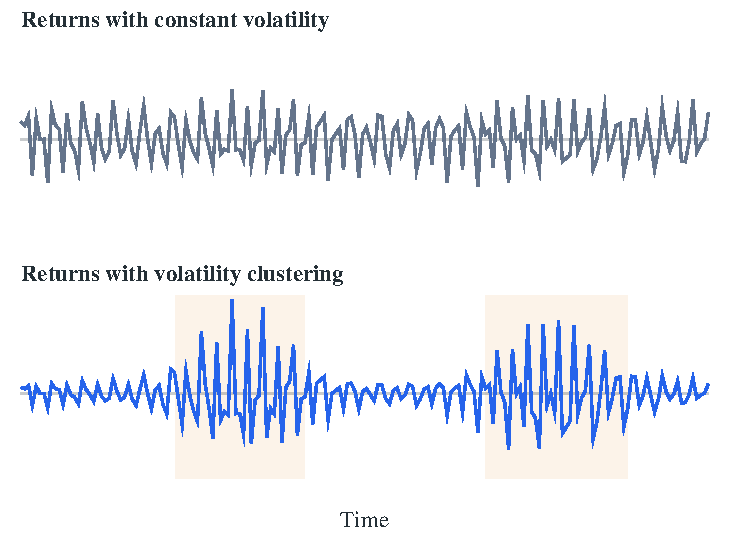
\includegraphics[width=\linewidth]{../reader_prototype/latex/figures/volatility.pdf}
\captionof{figure}{合成示意：右侧序列的收益率方向难以预测，但波动幅度具有明显的持续性。}
\end{readerfigure}

因此，在金融数据中，我们可能同时观察到：
\[\operatorname{Corr}(r_t,r_{t+h})\approx0,\]

但：
\[\operatorname{Corr}(|r_t|,|r_{t+h}|)>0,\]

或者：
\[\operatorname{Corr}(r_t^2,r_{t+h}^2)>0.\]

这意味着：

\textbf{收益率本身可能不具有明显的线性可预测性，但其波动程度具有可预测性。}

\begin{readerfigure}{0.87}
\figuretitle{Typical Financial Return ACF}
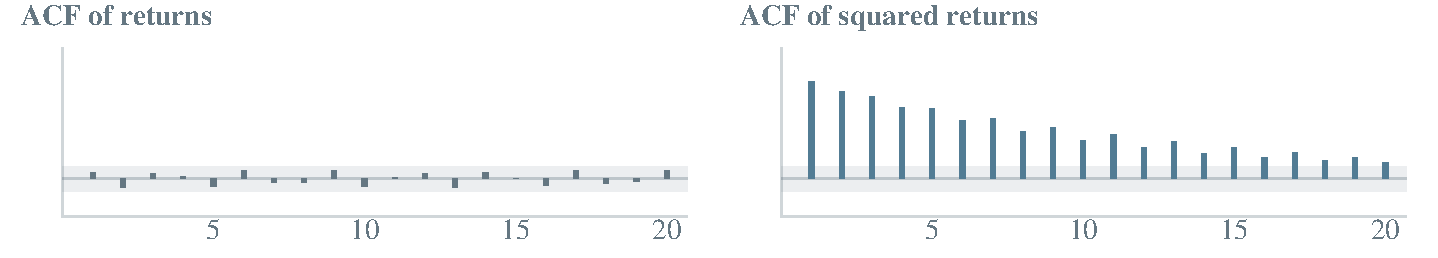
\includegraphics[width=\linewidth]{../reader_prototype/latex/figures/acf.pdf}
\captionof{figure}{典型形态的教学示意，非实际市场数据。原始收益率的自相关接近零，平方收益率的自相关则可能缓慢衰减。}
\end{readerfigure}

\hypertarget{part-4-58-0007-ux4e00ux4e2aux4e25ux683cux7684ux6982ux7387ux53cdux4f8b}{%
\subsubsection{6.3 一个严格的概率反例}\label{part-4-58-0007-ux4e00ux4e2aux4e25ux683cux7684ux6982ux7387ux53cdux4f8b}}

为了进一步理解为什么 Uncorrelated 不等于 Independent，我们构造一个非常简单的随机过程。 设：
\[Z_t\overset{\mathrm{i.i.d.}}{\sim}\mathcal N(0,1),\]

并定义：
\[r_t=Z_tZ_{t-1}.\]

首先，由独立性：
\[\mathbb E[r_t]
=
\mathbb E[Z_t]\mathbb E[Z_{t-1}]
=0.\]

\hypertarget{part-4-58-0007-proposition-1-returns-are-uncorrelated}{%
\paragraph{Proposition 1 --- Returns are uncorrelated}\label{part-4-58-0007-proposition-1-returns-are-uncorrelated}}

相邻收益率的协方差为：
\[\begin{aligned}
\operatorname{Cov}(r_t,r_{t+1})
&=\mathbb E[r_tr_{t+1}]\\
&=\mathbb E[Z_t^2Z_{t-1}Z_{t+1}]\\
&=\mathbb E[Z_t^2]
\mathbb E[Z_{t-1}]
\mathbb E[Z_{t+1}]\\
&=0.
\end{aligned}\]

因此：
\[\boxed{
\operatorname{Cov}(r_t,r_{t+1})=0.
}\]

\hypertarget{part-4-58-0007-proposition-2-squared-returns-are-correlated}{%
\paragraph{Proposition 2 --- Squared returns are correlated}\label{part-4-58-0007-proposition-2-squared-returns-are-correlated}}

现在考察平方收益率：
\[r_t^2=Z_t^2Z_{t-1}^2.\]

由于标准正态分布满足：
\[\mathbb E[Z_t^2]=1,
\qquad
\mathbb E[Z_t^4]=3,\]

所以：
\[\mathbb E[r_t^2]=1.\]

进一步：
\[\begin{aligned}
&\operatorname{Cov}(r_t^2,r_{t+1}^2)\\
&=\mathbb E[r_t^2r_{t+1}^2]
-\mathbb E[r_t^2]\mathbb E[r_{t+1}^2]\\
&=\mathbb E[Z_t^4Z_{t-1}^2Z_{t+1}^2]-1\\
&=\mathbb E[Z_t^4]
\mathbb E[Z_{t-1}^2]
\mathbb E[Z_{t+1}^2]-1\\
&=3-1\\
&=2.
\end{aligned}\]

于是：
\[\boxed{
\operatorname{Cov}(r_t^2,r_{t+1}^2)=2>0.
}\]

我们甚至可以进一步计算其平方收益率的相关系数。

由于：
\[\begin{aligned}
\operatorname{Var}(r_t^2)
&=\mathbb E[r_t^4]-\mathbb E[r_t^2]^2\\
&=3\times3-1\\
&=8,
\end{aligned}\]

因此：
\[\operatorname{Corr}(r_t^2,r_{t+1}^2)
=
\frac28
=
\frac14.\]

最终得到：
\[\boxed{
\begin{aligned}
\operatorname{Corr}(r_t,r_{t+1})&=0,\\
\operatorname{Corr}(r_t^2,r_{t+1}^2)&=0.25.
\end{aligned}
}\]

这严格证明了一个随机过程可以不存在收益率的线性相关性，却存在波动幅度的统计依赖。

当然，这只是一个概率论反例，而不是完整的金融市场模型。

\hypertarget{part-4-58-0007-arch-and-garch}{%
\subsubsection{6.4 ARCH and GARCH}\label{part-4-58-0007-arch-and-garch}}

为了描述 Volatility Clustering，金融计量经济学发展出了两种经典模型：

\begin{readertable}
\begin{longtable}[]{@{}
  >{\raggedright\arraybackslash}p{(\columnwidth - 4\tabcolsep) * \real{0.14}}
  >{\raggedright\arraybackslash}p{(\columnwidth - 4\tabcolsep) * \real{0.68}}
  >{\raggedleft\arraybackslash}p{(\columnwidth - 4\tabcolsep) * \real{0.14}}@{}}
\toprule
Model & Full Name & Year \\
\midrule
\endhead
ARCH & Autoregressive Conditional Heteroskedasticity & 1982 \\
GARCH & Generalized ARCH & 1986 \\
\bottomrule
\end{longtable}
\end{readertable}

目前只需要掌握 GARCH(1,1) 的基本结构。

\hypertarget{part-4-58-0007-model-definition}{%
\paragraph{Model Definition}\label{part-4-58-0007-model-definition}}

首先定义收益率：
\[r_t=\mu+\varepsilon_t,\]

其中：
\[\varepsilon_t=\sigma_tZ_t,\]

且 \(Z_t\) 是均值为 0、方差为 1 的 IID Innovation，并独立于过去的信息。

条件方差由下式决定：
\[\boxed{
\sigma_t^2
=
\omega
+a\varepsilon_{t-1}^2
+b\sigma_{t-1}^2
}\]

其中：
\[\omega>0,\qquad a,b\geq0.\]

\begin{readertable}
\begin{longtable}[]{@{}
  >{\raggedright\arraybackslash}p{(\columnwidth - 2\tabcolsep) * \real{0.27}}
  >{\raggedright\arraybackslash}p{(\columnwidth - 2\tabcolsep) * \real{0.69}}@{}}
\toprule
Parameter & Interpretation \\
\midrule
\endhead
\(\omega\) & 方差方程的常数项 \\
\(a\) & 对近期市场冲击的敏感程度 \\
\(b\) & 历史条件方差的持续程度 \\
\(a+b\) & 波动冲击在条件方差预测中的持续性 \\
\bottomrule
\end{longtable}
\end{readertable}

\begin{readerfigure}{0.53}
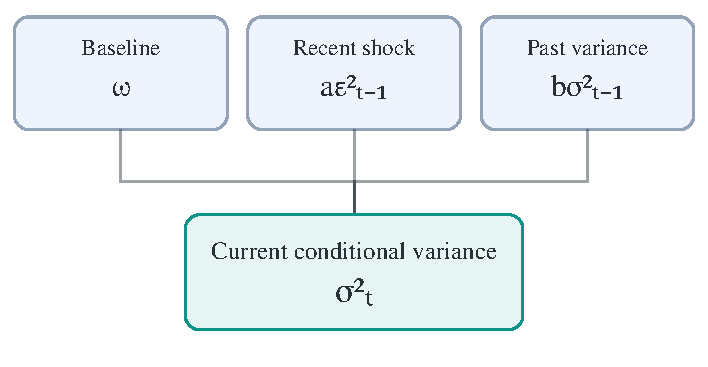
\includegraphics[width=\linewidth]{../reader_prototype/latex/figures/garch-mechanism.pdf}
\captionof{figure}{GARCH(1,1) 条件方差的组成}
\end{readerfigure}

GARCH 的基本思想是：当前波动率不仅取决于最近一次市场冲击，还受到此前波动率的影响。

\hypertarget{part-4-58-0007-proposition-unconditional-variance}{%
\paragraph{Proposition --- Unconditional Variance}\label{part-4-58-0007-proposition-unconditional-variance}}

假设存在具有有限二阶矩的平稳解，并满足：
\[a+b<1.\]

对条件方差方程两侧取期望：
\[\mathbb E[\sigma_t^2]
=
\omega
+a\mathbb E[\varepsilon_{t-1}^2]
+b\mathbb E[\sigma_{t-1}^2].\]

根据 Law of Total Expectation：
\[\begin{aligned}
\mathbb E[\varepsilon_{t-1}^2]
&=\mathbb E[
\mathbb E[\varepsilon_{t-1}^2
\mid\mathcal F_{t-2}]
]\\
&=\mathbb E[\sigma_{t-1}^2].
\end{aligned}\]

因此：
\[\mathbb E[\sigma_t^2]
=
\omega+(a+b)\mathbb E[\sigma_{t-1}^2].\]

由平稳性：
\[\mathbb E[\sigma_t^2]
=
\mathbb E[\sigma_{t-1}^2].\]

于是：
\[\boxed{
\mathbb E[\sigma_t^2]
=
\frac{\omega}{1-a-b}.
}\]

这同时也是上述模型中收益率的无条件方差。

\hypertarget{part-4-58-0007-volatility-persistence}{%
\paragraph{Volatility Persistence}\label{part-4-58-0007-volatility-persistence}}

设长期方差为：
\[\bar\sigma^2=\frac{\omega}{1-a-b}.\]

条件方差预测向长期方差回归的速度主要由 \(a+b\) 决定。

\begin{readerfigure}{0.72}
\figuretitle{GARCH --- Volatility Shock Persistence}
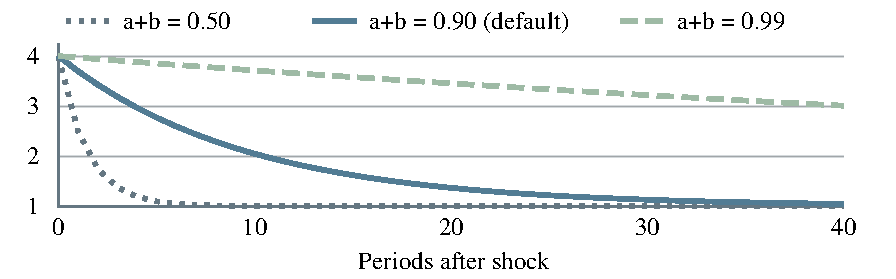
\includegraphics[width=\linewidth]{../reader_prototype/latex/figures/garch-persistence.pdf}

\smallskip
\begin{tabular}{@{}lrrr@{}}
\toprule
\(a+b\) & 0.50 & 0.90 & 0.99 \\
\midrule
Shock half-life（连续插值，Periods） & 1.00 & 6.58 & 68.97 \\
Remaining shock after 20 periods & 0.0\% & 12.2\% & 81.8\% \\
\bottomrule\end{tabular}
\captionof{figure}{归一化教学模型：长期方差为 1，初始超额方差为 3。曲线描述条件方差预测的恢复过程。}
\end{readerfigure}

这里有一个相当 Nontrivial 的观点：

\textbf{Conditional Variance 随时间变化，并不意味着 Unconditional Variance 随时间变化。}

GARCH 可以同时具有：

\begin{itemize}
\tightlist
\item
  Time-varying Conditional Variance；
\item
  Constant Unconditional Variance；
\item
  Weak Stationarity。
\end{itemize}

所以：
\[\boxed{
\text{Volatility Clustering}
\not\Rightarrow
\text{Non-stationarity}.
}\]

这一点非常容易混淆。

\hypertarget{part-4-58-0007-heavy-tailsux539aux5c3eux5206ux5e03}{%
\subsection{7. Heavy Tails（厚尾分布）}\label{part-4-58-0007-heavy-tailsux539aux5c3eux5206ux5e03}}

\hypertarget{part-4-58-0007-gaussian-assumption-ux7684ux5c40ux9650}{%
\subsubsection{7.1 Gaussian Assumption 的局限}\label{part-4-58-0007-gaussian-assumption-ux7684ux5c40ux9650}}

我们此前大量使用 Normal Distribution，因为它具有非常好的数学性质。

但是，现实金融收益率经常表现出比正态分布更厚的尾部，即极端观测值出现的概率比 Gaussian Model 所预期的更高。

\begin{readerfigure}{0.46}
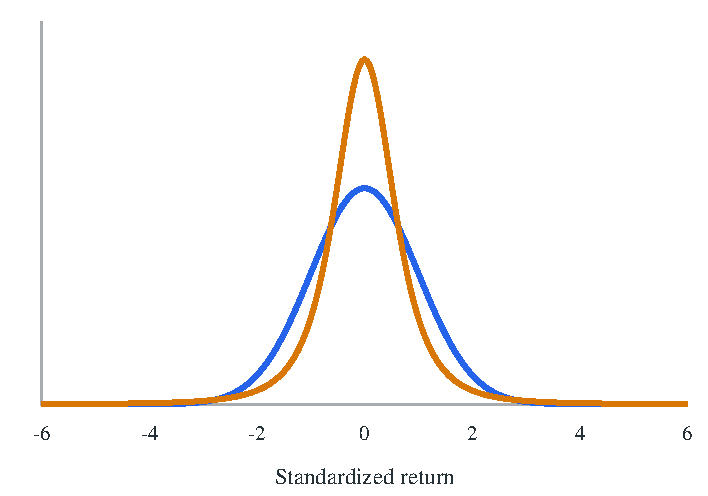
\includegraphics[width=\linewidth]{../reader_prototype/latex/figures/densities.pdf}
\par \legendmark{ResearchBlue}\,Standard Normal\enspace \legenddash{ResearchSlate}\,Standardized Student's t (ν=3)
\captionof{figure}{两种分布均具有零均值和单位方差，但尾部概率存在显著差异。}
\end{readerfigure}

例如，我们比较 Standard Normal Distribution 与标准化为单位方差的 Student's t Distribution（自由度为 3）。

\begin{readertable}
\begin{longtable}[]{@{}
  >{\raggedright\arraybackslash}p{(\columnwidth - 4\tabcolsep) * \real{0.33}}
  >{\raggedleft\arraybackslash}p{(\columnwidth - 4\tabcolsep) * \real{0.27}}
  >{\raggedleft\arraybackslash}p{(\columnwidth - 4\tabcolsep) * \real{0.36}}@{}}
\toprule
Extreme Event & Normal & Standardized \(t_3\) \\
\midrule
\endhead
超过 3 个标准差 & 0.270\% & 1.385\% \\
超过 5 个标准差 & 0.0000573\% & 0.324\% \\
\bottomrule
\end{longtable}
\end{readertable}

以上均为双侧理论尾部概率。

\begin{readerfigure}{0.72}
\figuretitle{Probability of a 5-standard-deviation event}
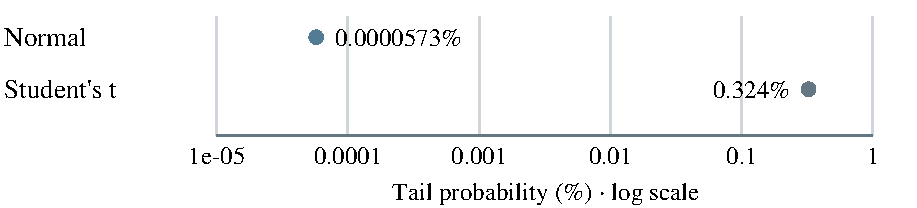
\includegraphics[width=\linewidth]{../reader_prototype/latex/figures/tail-probability.pdf}
\par\textbf{约 5,650 倍}
\captionof{figure}{即使均值和方差完全相同，极端事件概率也可能存在数量级差异。}
\end{readerfigure}

这也是为什么仅仅比较 Mean 和 Variance，可能不足以充分描述金融数据的风险特征。

\hypertarget{part-4-58-0007-moment-existenceux77e9ux7684ux5b58ux5728ux6027}{%
\subsubsection{7.2 Moment Existence（矩的存在性）}\label{part-4-58-0007-moment-existenceux77e9ux7684ux5b58ux5728ux6027}}

Student's t Distribution 具有一个值得关注的数学性质。

对于：
\[X\sim t_\nu,\]

其 \(p\) 阶绝对矩存在的条件为：
\[\boxed{
\mathbb E[|X|^p]<\infty
\iff p<\nu,
\qquad p>0.
}\]

\begin{readertable}
\begin{longtable}[]{@{}
  >{\raggedright\arraybackslash}p{(\columnwidth - 6\tabcolsep) * \real{0.33}}
  >{\raggedright\arraybackslash}p{(\columnwidth - 6\tabcolsep) * \real{0.16}}
  >{\raggedright\arraybackslash}p{(\columnwidth - 6\tabcolsep) * \real{0.20}}
  >{\raggedright\arraybackslash}p{(\columnwidth - 6\tabcolsep) * \real{0.27}}@{}}
\toprule
Degrees of Freedom & Mean & Variance & Fourth Moment \\
\midrule
\endhead
\(\nu=1\) & 不存在 & 不存在 & 不存在 \\
\(\nu=2\) & 存在 & 不存在 & 不存在 \\
\(\nu=3\) & 存在 & 存在 & 不存在 \\
\(\nu=5\) & 存在 & 存在 & 存在 \\
\bottomrule
\end{longtable}
\end{readertable}

其中：
\[t_1=\text{Cauchy Distribution}.\]

也就是此前 Probability 中学习过的 Cauchy Distribution。

\hypertarget{part-4-58-0007-proof-sketch}{%
\paragraph{Proof Sketch}\label{part-4-58-0007-proof-sketch}}

Student's t Distribution 的概率密度为：
\[f_\nu(x)
=
\frac{
\Gamma((\nu+1)/2)
}{
\sqrt{\nu\pi}\Gamma(\nu/2)
}
\left(1+\frac{x^2}{\nu}\right)^{-(\nu+1)/2}.\]

当 \(|x|\to\infty\) 时：
\[f_\nu(x)\asymp |x|^{-(\nu+1)}.\]

因此，绝对矩积分的尾部行为为：
\[\int^\infty x^pf_\nu(x)\,\mathrm dx
\asymp
\int^\infty x^{p-\nu-1}\,\mathrm dx.\]

根据 Improper Integral 的收敛条件：
\[p-\nu-1<-1,\]

即：
\[\boxed{p<\nu.}\]

\hypertarget{part-4-58-0007-heavy-tails-ux5bf9ux7edfux8ba1ux5b66ux4e60ux7684ux5f71ux54cd}{%
\subsubsection{7.3 Heavy Tails 对统计学习的影响}\label{part-4-58-0007-heavy-tails-ux5bf9ux7edfux8ba1ux5b66ux4e60ux7684ux5f71ux54cd}}

现在回顾 Part II 中使用过的几个数学工具。

\begin{readertable}
\begin{longtable}[]{@{}
  >{\raggedright\arraybackslash}p{(\columnwidth - 4\tabcolsep) * \real{0.32}}
  >{\raggedright\arraybackslash}p{(\columnwidth - 4\tabcolsep) * \real{0.29}}
  >{\raggedright\arraybackslash}p{(\columnwidth - 4\tabcolsep) * \real{0.35}}@{}}
\toprule
Statistical Tool & Relevant Assumption & Potential Problem \\
\midrule
\endhead
Chebyshev Inequality & Finite Variance & 方差可能不存在 \\
Classical IID CLT & Finite Variance & 极限分布可能不是正态 \\
Hoeffding Inequality & Bounded Variables & 收益率或损失函数可能无界 \\
Sample Variance Inference & 通常涉及高阶矩条件 & 方差估计本身可能非常不稳定 \\
Standard Bootstrap & 依赖统计量及分布条件 & 厚尾可能影响重采样推断 \\
\bottomrule
\end{longtable}
\end{readertable}

尤其需要注意一种情况：

假设预测误差具有有限二阶矩，却没有有限四阶矩。

那么对于 Squared Loss：
\[L=\varepsilon^2,\]

我们可能有：
\[\mathbb E[L]=\mathbb E[\varepsilon^2]<\infty,\]

但：
\[\operatorname{Var}(L)
=
\mathbb E[\varepsilon^4]
-\mathbb E[\varepsilon^2]^2
=\infty.\]

也就是说，\textbf{Population MSE 可以存在，但经验 MSE 的方差可能不存在。}

这使得两个模型之间微小的 MSE Improvement 更难被可靠识别。

对于 Financial RSI，Agent 可能不断根据高度不稳定的 Evaluation Score 修改自身，并将偶然出现的极端结果误认为真实研究规律。

当然，金融数据具有厚尾，并不意味着它一定没有有限方差。上述结论取决于具体 DGP 与所使用的损失函数。

\hypertarget{part-4-58-0007-temporal-dependence-and-effective-sample-size}{%
\subsection{8. Temporal Dependence and Effective Sample Size}\label{part-4-58-0007-temporal-dependence-and-effective-sample-size}}

这是本阶段与 Part II 联系最紧密的数学内容之一。

\hypertarget{part-4-58-0007-ux4e2aux89c2ux6d4bux503cux4e0dux4e00ux5b9aux5bf9ux5e94-1000-ux4efdux72ecux7acbux4fe1ux606f}{%
\subsubsection{8.1 1,000 个观测值不一定对应 1,000 份独立信息}\label{part-4-58-0007-ux4e2aux89c2ux6d4bux503cux4e0dux4e00ux5b9aux5bf9ux5e94-1000-ux4efdux72ecux7acbux4fe1ux606f}}

对于 IID Random Variables：
\[\operatorname{Var}(\bar X_n)
=
\frac{\sigma^2}{n}.\]

然而，当观测值存在时间依赖时，这个关系不再普遍成立。

设 \(\{X_t\}\) 为弱平稳随机过程，并定义：
\[\gamma_h
=
\operatorname{Cov}(X_t,X_{t+h}),\]

\[\rho_h=\frac{\gamma_h}{\gamma_0}.\]

那么：
\[\boxed{
\operatorname{Var}(\bar X_n)
=
\frac{\gamma_0}{n}
\left[
1+
2\sum_{h=1}^{n-1}
\left(1-\frac hn\right)\rho_h
\right].
}\]

这实际上就是我们在 II-F 中使用过的时间序列样本均值方差公式。

\hypertarget{part-4-58-0007-proof}{%
\paragraph{Proof}\label{part-4-58-0007-proof}}

\[\begin{aligned}
\operatorname{Var}(\bar X_n)
&=
\operatorname{Var}
\left(
\frac1n\sum_{t=1}^nX_t
\right)\\
&=\frac1{n^2}
\sum_{i=1}^n
\sum_{j=1}^n
\operatorname{Cov}(X_i,X_j).
\end{aligned}\]

利用弱平稳性，将相同 Lag 的协方差项合并：
\[\operatorname{Var}(\bar X_n)
=
\frac1{n^2}
\left[
n\gamma_0
+2\sum_{h=1}^{n-1}(n-h)\gamma_h
\right].\]

提取公因子即可得到上述结果。

\hypertarget{part-4-58-0007-effective-sample-size}{%
\subsubsection{8.2 Effective Sample Size}\label{part-4-58-0007-effective-sample-size}}

为了刻画时间依赖对样本均值估计的影响，我们定义：
\[\boxed{
n_{\mathrm{eff}}
=
\frac{n}{
1+
2\sum_{h=1}^{n-1}
(1-h/n)\rho_h
}.
}\]

在分母为正的条件下，有：
\[\operatorname{Var}(\bar X_n)
=
\frac{\gamma_0}{n_{\mathrm{eff}}}.\]

这里的 \(n_{\mathrm{eff}}\) 称为 Effective Sample Size（有效样本量）。

其含义是：对于样本均值估计，当前相关序列的方差，相当于多少个具有相同边际方差的独立观测值所产生的方差。

需要注意，Effective Sample Size 是针对具体统计量定义的，并不是一份数据集唯一且固定的属性。

\hypertarget{part-4-58-0007-ar1-example}{%
\subsubsection{8.3 AR(1) Example}\label{part-4-58-0007-ar1-example}}

沿用 §5.2 中的模型：
\[X_t=\phi X_{t-1}+\varepsilon_t,\]

其中：
\[|\phi|<1.\]

我们已经得到：
\[\rho_h=\phi^{|h|}.\]

当 \(n\) 足够大、\(\phi\) 固定时：
\[\begin{aligned}
1+2\sum_{h=1}^{\infty}\phi^h
&=1+\frac{2\phi}{1-\phi}\\
&=\frac{1+\phi}{1-\phi}.
\end{aligned}\]

因此：
\[\boxed{
n_{\mathrm{eff}}
\approx
n\frac{1-\phi}{1+\phi}.
}\]

\textbf{Effective Sample Size Explorer}

Nominal sample size \(n\)\\
\textbf{1,000}

1000（范围 100--5000）

Autocorrelation parameter \(\phi\)\\
\textbf{0.80}

0.8（范围 0--0.95）

Nominal sample size

\begin{verbatim}
  **1,000**
\end{verbatim}

Effective sample size

\begin{verbatim}
  **112**
\end{verbatim}

Effective information ratio

\textbf{11.2\%}

Standard error multiplier

\textbf{2.99×}

基于平稳 AR(1) 的有限样本方差公式计算，而非真实金融市场的估计结果。

对于 \(n=1000\)，可以得到如下渐近近似结果。

\begin{readertable}
\begin{longtable}[]{@{}
  >{\raggedleft\arraybackslash}p{(\columnwidth - 4\tabcolsep) * \real{0.15}}
  >{\raggedleft\arraybackslash}p{(\columnwidth - 4\tabcolsep) * \real{0.39}}
  >{\raggedleft\arraybackslash}p{(\columnwidth - 4\tabcolsep) * \real{0.42}}@{}}
\toprule
\(\phi\) & Nominal Sample Size & Effective Sample Size \\
\midrule
\endhead
0.0 & 1,000 & 1,000 \\
0.2 & 1,000 & 667 \\
0.5 & 1,000 & 333 \\
0.8 & 1,000 & 111 \\
0.9 & 1,000 & 53 \\
0.95 & 1,000 & 26 \\
\bottomrule
\end{longtable}
\end{readertable}

因此，较强的正向时间依赖可能显著降低有效样本信息量。负自相关则可能使针对样本均值定义的有效样本量超过原始样本量。

\hypertarget{part-4-58-0007-ux4e00ux4e2aux4e0e-rsi-ux76f4ux63a5ux76f8ux5173ux7684-nontrivial-example}{%
\subsubsection{8.4 一个与 RSI 直接相关的 Nontrivial Example}\label{part-4-58-0007-ux4e00ux4e2aux4e0e-rsi-ux76f4ux63a5ux76f8ux5173ux7684-nontrivial-example}}

假设我们的金融预测任务使用未来五期的累计 Log Return 作为 Label。

定义：
\[Y_t=\sum_{j=1}^{5}r_{t+j}^{\log}.\]

为了简化分析，假设单期 Log Return 为 IID：
\[r_t^{\log}\sim(0,\sigma^2).\]

即使原始收益率完全独立，相邻 Label 仍然存在重叠。

\textbf{Overlapping Return Labels}

\bookgraphic{0.693}{part-4-58-0007-008-01}{相邻五期累计收益率共享四个原始收益率观测值。}

由于：
\[Y_t=r_{t+1}^{\log}+\cdots+r_{t+5}^{\log},\]

\[Y_{t+1}=r_{t+2}^{\log}+\cdots+r_{t+6}^{\log},\]

因此：
\[\operatorname{Cov}(Y_t,Y_{t+1})
=
4\sigma^2.\]

又因为：
\[\operatorname{Var}(Y_t)=5\sigma^2,\]

所以：
\[\boxed{
\operatorname{Corr}(Y_t,Y_{t+1})
=
\frac45=0.8.
}\]

更加一般地，对于长度为 \(H\) 的累计 Log Return：
\[Y_t=\sum_{j=1}^{H}r_{t+j}^{\log},\]

在上述 IID 假设下：
\[\boxed{
\rho_h=
\begin{cases}
1-\dfrac{|h|}{H},&|h|<H,\\
0,&|h|\geq H.
\end{cases}
}\]

因此，当 \(n\) 足够大时：
\[\begin{aligned}
n_{\mathrm{eff}}
&\approx
\frac{n}{
1+2\sum_{h=1}^{H-1}(1-h/H)
}\\
&=\frac{n}{H}.
\end{aligned}\]

也就是说：
\[\boxed{
n_{\mathrm{eff}}\approx\frac nH.
}\]

假如我们拥有 1,000 个相互重叠的 20 日收益率标签，其均值估计的有效样本量可能仅相当于约 50 个独立标签。

这也进一步解释了 II-F 中为什么需要 Purging、Label Availability Check 和 dependence-aware Statistical Inference。 注意：这个有效样本量公式针对上述 IID 增量模型中的标签均值，不能直接套用到所有模型损失或策略收益上。

\hypertarget{part-4-58-0007-ux4e3aux4ec0ux4e48ux91d1ux878dux73afux5883ux7279ux522bux5bb9ux6613ux4ea7ux751f-rsi-overfitting}{%
\subsection{9. 为什么金融环境特别容易产生 RSI Overfitting？}\label{part-4-58-0007-ux4e3aux4ec0ux4e48ux91d1ux878dux73afux5883ux7279ux522bux5bb9ux6613ux4ea7ux751f-rsi-overfitting}}

现在可以将本阶段的内容与 Part II 和 Part III 连接起来。

\begin{readertable}
\begin{longtable}[]{@{}
  >{\raggedright\arraybackslash}p{(\columnwidth - 4\tabcolsep) * \real{0.29}}
  >{\raggedright\arraybackslash}p{(\columnwidth - 4\tabcolsep) * \real{0.31}}
  >{\raggedright\arraybackslash}p{(\columnwidth - 4\tabcolsep) * \real{0.37}}@{}}
\toprule
Financial Property & Statistical Consequence & RSI Consequence \\
\midrule
\endhead
Weak Predictability & 真实模型差异可能很小 & 容易选择噪声驱动的修改 \\
Temporal Dependence & 有效样本信息可能减少 & 评估可靠性下降 \\
Heavy Tails & 极端观测可能主导指标 & Agent 可能过度优化偶然事件 \\
Volatility Clustering & 条件方差随时间变化 & 不同市场窗口的评分稳定性不同 \\
Non-stationarity & 历史规律可能失效 & 后期版本可能过度适应旧环境 \\
Single Historical Path & 缺少独立市场历史 & 反复回测可能累积选择偏差 \\
\bottomrule
\end{longtable}
\end{readertable}

\textbf{Coding Tasks}

部分正确性可以确定性验证

反馈相对明确

\textbf{Financial Tasks}

真实性能难以直接观测

评估反馈可能包含大量噪声

↓

\textbf{Same RSI Architecture} \(A_0\rightarrow A_1\rightarrow\cdots\rightarrow A_K\)

↓

\bookgraphic{0.591}{part-4-58-0007-009-01}{}

IS Performance

Potential OOS trajectory in a reliable evaluation environment

Potential OOS trajectory in a low-SNR financial environment

研究假设示意，并非真实实验结果。编程任务同样可能发生严重过拟合。

这里最重要的认识是：

\textbf{金融环境未必削弱 Agent 的 Optimization Capability，却可能显著削弱 Evaluator 区分真实改进与虚假改进的能力。}

Agent 仍然可以变得越来越擅长搜索，但它所搜索到的高分候选未必代表真正的能力提升。

\hypertarget{part-4-58-0007-research-practice-initial-financial-data-audit}{%
\subsection{10. Research Practice --- Initial Financial Data Audit}\label{part-4-58-0007-research-practice-initial-financial-data-audit}}

假设未来课题组向我们提供了一份金融数据，我们不应该立即开始运行 RSI。

第一步应当对 DGP 的统计特征进行初步分析。

\hypertarget{part-4-58-0007-diagnostic-framework}{%
\subsubsection{10.1 Diagnostic Framework}\label{part-4-58-0007-diagnostic-framework}}

\begin{readertable}
\begin{longtable}[]{@{}
  >{\raggedright\arraybackslash}p{(\columnwidth - 4\tabcolsep) * \real{0.32}}
  >{\raggedright\arraybackslash}p{(\columnwidth - 4\tabcolsep) * \real{0.37}}
  >{\raggedright\arraybackslash}p{(\columnwidth - 4\tabcolsep) * \real{0.27}}@{}}
\toprule
Diagnostic & Method & Research Purpose \\
\midrule
\endhead
Return Transformation & Simple / Log Return & 统一统计对象 \\
Distribution Analysis & Histogram、Q-Q Plot & 检查厚尾及偏度 \\
Temporal Dependence & ACF of Returns & 检查线性依赖 \\
Volatility Dependence & ACF of Absolute / Squared Returns & 检查波动率聚集 \\
Rolling Statistics & Rolling Mean / Variance & 调查潜在结构变化 \\
Information Availability & Timestamp Audit & 排除 Look-Ahead Bias \\
Sample Size Analysis & Effective Sample Size & 判断评估不确定性 \\
\bottomrule
\end{longtable}
\end{readertable}

\hypertarget{part-4-58-0007-python-implementation}{%
\subsubsection{10.2 Python Implementation}\label{part-4-58-0007-python-implementation}}

一个基本的 Exploratory Data Analysis 可以写成：

\begin{verbatim}
import numpy as np
import pandas as pd
import matplotlib.pyplot as plt

from statsmodels.graphics.tsaplots import plot_acf
from scipy.stats import probplot

# Assume df contains chronologically indexed prices.
df = df.sort_index()

# Log returns
r = np.log(df["close"]).diff().dropna()

fig, axes = plt.subplots(2, 3, figsize=(14, 7))

# 1. Distribution
axes[0, 0].hist(r, bins=60, density=True)
axes[0, 0].set_title("Return Distribution")

# 2. Normal Q-Q plot
probplot(r, dist="norm", plot=axes[0, 1])
axes[0, 1].set_title("Normal Q-Q Plot")

# 3. Rolling volatility
r.rolling(60).std().plot(ax=axes[0, 2])
axes[0, 2].set_title("Rolling Volatility")

# 4. Return autocorrelation
plot_acf(r, lags=30, ax=axes[1, 0])
axes[1, 0].set_title("ACF of Returns")

# 5. Absolute return autocorrelation
plot_acf(r.abs(), lags=30, ax=axes[1, 1])
axes[1, 1].set_title("ACF of Absolute Returns")

# 6. Squared return autocorrelation
plot_acf(r**2, lags=30, ax=axes[1, 2])
axes[1, 2].set_title("ACF of Squared Returns")

plt.tight_layout()
plt.show()
\end{verbatim}

这段代码尚未在课题组数据上实际运行，假设价格为正且数据量足够。实际使用时需要处理复权价格、缺失值、交易日对齐及 ACF 置信区间的适用条件。

尤其需要注意，如果这些探索性分析将用于设计 RSI 策略，那么应该只在 Development Dataset 上进行，而不是提前分析封闭的 Final Test Dataset。

否则，人类研究人员也可能发生我们在 II-F 中讨论过的 Researcher-level Overfitting。

\hypertarget{part-4-58-0007-literature-index}{%
\subsection{11. Literature Index}\label{part-4-58-0007-literature-index}}

本阶段不需要立刻学习完整的 Financial Econometrics 教材，优先掌握以下经典文献即可。

\textbf{P0 --- Empirical Properties of Asset Returns: Stylized Facts and Statistical Issues}

Rama Cont · 2001 · Quantitative Finance, 1(2), 223--236 · 同行评审

本阶段最重要的参考文献。重点理解收益率分布、非线性依赖、Volatility Clustering 和金融统计估计困难。

\href{https://doi.org/10.1080/713665670}{DOI: 10.1080/713665670}

\textbf{P1 --- Generalized Autoregressive Conditional Heteroskedasticity}

Tim Bollerslev · 1986 · Journal of Econometrics, 31(3), 307--327 · 同行评审

GARCH 的经典原始论文。现阶段理解 Model Specification 与 Stationarity 即可，不需要深入 Maximum Likelihood Estimation。

\href{https://doi.org/10.1016/0304-4076(86)90063-1}{DOI: 10.1016/0304-4076(86)90063-1}

本次补发没有重新进行文献检索。这里保留上述两篇经典文献作为主要阅读入口。

\hypertarget{part-4-58-0007-iv-a-conclusion-index}{%
\subsection{12. IV-A --- Conclusion Index}\label{part-4-58-0007-iv-a-conclusion-index}}

\hypertarget{part-4-58-0007-core-conclusions}{%
\subsubsection{12.1 Core Conclusions}\label{part-4-58-0007-core-conclusions}}

\begin{readertable}
\begin{longtable}[]{@{}
  >{\raggedright\arraybackslash}p{(\columnwidth - 4\tabcolsep) * \real{0.13}}
  >{\raggedright\arraybackslash}p{(\columnwidth - 4\tabcolsep) * \real{0.70}}
  >{\raggedright\arraybackslash}p{(\columnwidth - 4\tabcolsep) * \real{0.13}}@{}}
\toprule
ID & Key Conclusion & Index \\
\midrule
\endhead
A1 & Simple Return 通过乘法累积，Log Return 通过加法累积 & §1 \\
A2 & 一条历史序列只是随机过程的一条 Sample Path & §2.1 \\
A3 & Filtration 定义金融预测中的合法信息集合 & §2.2 \\
A4 & Conditional Mean 与 Conditional Variance 是不同预测目标 & §3 \\
A5 & Stationarity 不等于 Independence & §4 \\
A6 & Random Walk 的价格非平稳，但其增量可以平稳 & §4.3 \\
A7 & ACF 衡量时间序列的线性依赖 & §5 \\
A8 & 零自相关不意味着不存在非线性时间依赖 & §6.3 \\
A9 & Volatility Clustering 不必然意味着 Non-stationarity & §6.4 \\
A10 & Heavy Tails 可能限制传统统计推断方法的适用性 & §7 \\
A11 & Temporal Dependence 会改变有效样本信息量 & §8 \\
A12 & 金融数据特性可能降低 RSI Evaluator 的可靠性 & §9 \\
\bottomrule
\end{longtable}
\end{readertable}

\hypertarget{part-4-58-0007-core-formula-sheet}{%
\subsubsection{12.2 Core Formula Sheet}\label{part-4-58-0007-core-formula-sheet}}

\hypertarget{part-4-58-0007-result-1-return-transformation}{%
\paragraph{Result 1 --- Return Transformation}\label{part-4-58-0007-result-1-return-transformation}}

\[r_t=\frac{P_t-P_{t-1}}{P_{t-1}},\]

\[r_t^{\log}=\log(1+r_t).\]

\hypertarget{part-4-58-0007-result-2-financial-dgp}{%
\paragraph{Result 2 --- Financial DGP}\label{part-4-58-0007-result-2-financial-dgp}}

\[r_{t+1}
=
\mu_t+\sigma_tZ_{t+1}.\]

\hypertarget{part-4-58-0007-result-3-ar1}{%
\paragraph{Result 3 --- AR(1)}\label{part-4-58-0007-result-3-ar1}}

\[X_t=\phi X_{t-1}+\varepsilon_t.\]

在相应平稳条件下：
\[\operatorname{Var}(X_t)
=
\frac{\sigma_\varepsilon^2}{1-\phi^2},\]

\[\rho_h=\phi^{|h|}.\]

\hypertarget{part-4-58-0007-result-4-garch11}{%
\paragraph{Result 4 --- GARCH(1,1)}\label{part-4-58-0007-result-4-garch11}}

\[\sigma_t^2
=
\omega+a\varepsilon_{t-1}^2+b\sigma_{t-1}^2.\]

在有限二阶矩平稳条件下：
\[\boxed{
\mathbb E[\sigma_t^2]
=
\frac{\omega}{1-a-b}.
}\]

\hypertarget{part-4-58-0007-result-5-moment-existence-of-students-t}{%
\paragraph{Result 5 --- Moment Existence of Student's t}\label{part-4-58-0007-result-5-moment-existence-of-students-t}}

\[X\sim t_\nu
\quad\Longrightarrow\quad
\mathbb E[|X|^p]<\infty
\iff p<\nu.\]

\hypertarget{part-4-58-0007-result-6-effective-sample-size}{%
\paragraph{Result 6 --- Effective Sample Size}\label{part-4-58-0007-result-6-effective-sample-size}}

\[n_{\mathrm{eff}}
=
\frac{n}{
1+2\sum_{h=1}^{n-1}(1-h/n)\rho_h
}.\]

对于平稳 AR(1)：
\[\boxed{
n_{\mathrm{eff}}
\approx
n\frac{1-\phi}{1+\phi}.
}\]

\hypertarget{part-4-58-0007-result-7-overlapping-return-labels}{%
\paragraph{Result 7 --- Overlapping Return Labels}\label{part-4-58-0007-result-7-overlapping-return-labels}}

对于 IID 单期收益率构成的 \(H\) 期累计收益率标签：
\[\rho_h=
\begin{cases}
1-\dfrac{|h|}{H},&|h|<H,\\
0,&|h|\geq H.
\end{cases}\]

当 \(n\) 足够大时，针对标签均值：
\[\boxed{
n_{\mathrm{eff}}\approx\frac nH.
}\]

\hypertarget{part-4-58-0007-proof-index}{%
\subsubsection{12.3 Proof Index}\label{part-4-58-0007-proof-index}}

如果第二轮学习时希望重点复习数学推导，可以直接索引下表。

\begin{readertable}
\begin{longtable}[]{@{}
  >{\raggedright\arraybackslash}p{(\columnwidth - 4\tabcolsep) * \real{0.14}}
  >{\raggedright\arraybackslash}p{(\columnwidth - 4\tabcolsep) * \real{0.61}}
  >{\raggedright\arraybackslash}p{(\columnwidth - 4\tabcolsep) * \real{0.20}}@{}}
\toprule
Proof & Mathematical Result & Location \\
\midrule
\endhead
P1 & Log Return 的 Time Additivity & §1.3 \\
P2 & Random Walk 的 Non-stationarity & §4.3 \\
P3 & 零自相关但平方序列相关的反例 & §6.3 \\
P4 & GARCH 的 Unconditional Variance & §6.4 \\
P5 & Student's t 的矩存在条件 & §7.2 \\
P6 & 相关序列的样本均值方差 & §8.1 \\
P7 & AR(1) 的 Effective Sample Size & §8.3 \\
P8 & Overlapping Labels 的相关性及有效样本量 & §8.4 \\
\bottomrule
\end{longtable}
\end{readertable}

\hypertarget{part-4-58-0007-research-takeaway}{%
\subsection{13. Research Takeaway}\label{part-4-58-0007-research-takeaway}}

将整个 IV-A 压缩为一个核心观点：

\textbf{金融 RSI 面临的困难，不仅是需要从高噪声数据中寻找规律，还需要在同一批有限、相关且可能非平稳的数据中，反复判断哪些研究修改是真正有效的。}

我们可以用如下概念关系将其与之前的内容连接起来。

\textbf{Agent Capability}

Part III

Search、Memory、RSI

\textbf{Evaluator Reliability}

Part II + Part IV

Statistics、Financial DGP

↓

\textbf{Optimization--Evaluation Mismatch}

优化能力提高的速度可能超过评价机制可靠性提高的速度

↓

\textbf{Potential Generalization Decay} \(S_k^{\mathrm{IS}}\uparrow,\qquad S_k^{\mathrm{OOS}}\downarrow\)

这仍然是一种需要受控实验验证的研究假设，而不是金融 RSI 必然遵守的定律。

\hypertarget{part-4-58-0007-next-iv-b-low-signal-to-noise-ratio-predictability}{%
\subsection{Next --- IV-B: Low Signal-to-Noise Ratio \& Predictability}\label{part-4-58-0007-next-iv-b-low-signal-to-noise-ratio-predictability}}

IV-A --- Financial Time Series \& DGP

IV-B --- Low Signal-to-Noise Ratio \& Predictability

IV-C --- Financial Factors \& ML Models

IV-D --- Returns, Sharpe Ratio \& Evaluation

IV-E --- Backtest Overfitting, PBO \& DSR

IV-F --- Market Regime \& Robustness

下一阶段是 Part IV 中理论优先级最高的一节。

\begin{readertable}
\begin{longtable}[]{@{}
  >{\raggedright\arraybackslash}p{(\columnwidth - 2\tabcolsep) * \real{0.41}}
  >{\raggedright\arraybackslash}p{(\columnwidth - 2\tabcolsep) * \real{0.55}}@{}}
\toprule
Topic & Core Question \\
\midrule
\endhead
Signal-to-Noise Ratio & 如何定量描述金融预测的困难？ \\
Law of Total Variance & 如何分解可预测与不可预测成分？ \\
Irreducible Error & 模型性能的理论上限在哪里？ \\
Bayes Optimal Predictor & 最好的预测器在数学上是什么？ \\
Population \(R^2\) & 低信噪比如何限制预测能力？ \\
Efficient Market Hypothesis & 为什么金融规律可能难以持续利用？ \\
Spurious Correlation & 为什么无效金融特征也可能获得极高得分？ \\
Noise-driven Optimization & RSI 如何逐步将噪声误认为真实改进？ \\
\bottomrule
\end{longtable}
\end{readertable}

特别是，我们将利用你已经掌握的 Conditional Expectation 与 Law of Total Variance 推导：
\[\boxed{
R_{\mathrm{optimal}}^2
=
\frac{\mathrm{SNR}}{1+\mathrm{SNR}}
}\]

\textbf{Signal-to-Noise Ratio vs. Optimal Predictability}

\bookgraphic{0.473}{part-4-58-0007-013-01}{理论关系预览：在平方损失、有限二阶矩及特定 SNR 定义下成立。}

这个等式将金融数据的信噪比与理论最优预测能力直接联系起来。

而 IV-B 真正值得研究的地方就在于：\textbf{即使 Agent 具有无限强大的优化能力，它也无法突破给定信息集合所决定的理论预测上限。}

% Archive record 60, line 1.
\hypertarget{part-4-60-0001-iv-b-low-signal-to-noise-ratio-predictability}{%
\section{IV-B --- Low Signal-to-Noise Ratio \& Predictability}\label{part-4-60-0001-iv-b-low-signal-to-noise-ratio-predictability}}

这是 Part IV 中理论优先级最高的一节，也是整个 X Program \#161 研究动机的核心组成部分。

上一阶段 IV-A 介绍了金融数据的基本统计性质，但还有一个更加本质的问题：

\textbf{假设我们拥有一个能力极强的 AI Research Agent，并且允许它不断改进自身，它究竟能够在多大程度上提高金融预测能力？}

这里需要区分两种完全不同的限制：

\begin{readertable}
\begin{longtable}[]{@{}
  >{\raggedright\arraybackslash}p{(\columnwidth - 4\tabcolsep) * \real{0.31}}
  >{\raggedright\arraybackslash}p{(\columnwidth - 4\tabcolsep) * \real{0.34}}
  >{\raggedright\arraybackslash}p{(\columnwidth - 4\tabcolsep) * \real{0.30}}@{}}
\toprule
Limitation & 含义 & 能否通过 RSI 改善？ \\
\midrule
\endhead
Computational Limitation & 搜索能力不足、模型不够复杂 & 可能 \\
Statistical Limitation & 有限数据导致估计误差 & 可能缓解 \\
Information Limitation & 已知信息本身不足以预测未来 & 固定信息集合下无法突破 \\
\bottomrule
\end{longtable}
\end{readertable}

前两个问题主要涉及我们在 Part II 和 Part III 中学习的知识。

第三个问题，就是本阶段研究的重点。

我们将利用 Conditional Expectation、Law of Total Variance、Regression 和 Hypothesis Testing，建立一套关于金融可预测性的数学框架。

\hypertarget{part-4-60-0001-signal-and-noiseux4fe1ux53f7ux4e0eux566aux58f0}{%
\subsection{1. Signal and Noise（信号与噪声）}\label{part-4-60-0001-signal-and-noiseux4fe1ux53f7ux4e0eux566aux58f0}}

\hypertarget{part-4-60-0001-financial-data-generating-process}{%
\subsubsection{1.1 Financial Data Generating Process}\label{part-4-60-0001-financial-data-generating-process}}

沿用此前的记号：
\[\boxed{
r_{t+1}=g(X_t)+\varepsilon_{t+1}
}\]

其中：

\begin{itemize}
\tightlist
\item
  \(r_{t+1}\)：下一期收益率；
\item
  \(X_t\)：时刻 \(t\) 可以获得的特征；
\item
  \(g(X_t)\)：收益率中能够通过这些特征预测的部分；
\item
  \(\varepsilon_{t+1}\)：无法通过这些特征预测的随机成分。
\end{itemize}

为了使这种分解具有明确的数学含义，我们定义：
\[g(X_t)
=
\mathbb E[r_{t+1}\mid X_t].\]

于是：
\[\boxed{
\mathbb E[\varepsilon_{t+1}\mid X_t]=0.
}\]

如果 \(X_t\) 还充分包含了预测条件均值所需的历史信息，那么也可以进一步得到：
\[g(X_t)=
\mathbb E[r_{t+1}\mid\mathcal F_t].\]

但后者需要额外的信息充分性条件，并非自动成立。

\textbf{Signal--Noise Decomposition}

\bookgraphic{0.386}{part-4-60-0001-001-01}{}

\[r_{t+1}=\underbrace{g(X_t)}_{\text{Signal}}+\underbrace{\varepsilon_{t+1}}_{\text{Noise}}\]

合成教学示意，三幅图采用相同纵轴尺度。现实中只能观察到收益率，真实 Signal 通常是未知的。

金融预测的困难在于：我们观察到的并不是 Signal 本身，而是被大量 Noise 覆盖后的结果。

\hypertarget{part-4-60-0001-signal-to-noise-ratio-snr}{%
\subsubsection{1.2 Signal-to-Noise Ratio (SNR)}\label{part-4-60-0001-signal-to-noise-ratio-snr}}

在有限二阶矩的条件下，我们定义方差信噪比：
\[\boxed{
\mathrm{SNR}
=
\frac{\operatorname{Var}(g(X_t))}
{\operatorname{Var}(\varepsilon_{t+1})}
}\]

其中假设噪声方差大于零。

SNR 衡量的是可预测成分相对于不可预测成分的波动强度。

\begin{readertable}
\begin{longtable}[]{@{}
  >{\raggedleft\arraybackslash}p{(\columnwidth - 4\tabcolsep) * \real{0.16}}
  >{\raggedleft\arraybackslash}p{(\columnwidth - 4\tabcolsep) * \real{0.43}}
  >{\raggedright\arraybackslash}p{(\columnwidth - 4\tabcolsep) * \real{0.37}}@{}}
\toprule
SNR & Signal : Noise Variance & Interpretation \\
\midrule
\endhead
10 & 10 : 1 & Signal-dominated \\
1 & 1 : 1 & 两者方差相同 \\
0.1 & 1 : 10 & Noise-dominated \\
0.01 & 1 : 100 & Very low SNR \\
0.001 & 1 : 1,000 & Extremely low SNR \\
\bottomrule
\end{longtable}
\end{readertable}

这里使用的是方差之比，而不是标准差之比。不同学科可能采用其他 SNR 定义，后续所有推导均以本节定义为准。

\textbf{Signal-to-Noise Ratio Explorer}

Log-scale SNR\\
\textbf{0.01}

-2（范围 -3--1）

Predictable variance

\textbf{0.99\%}

Unpredictable variance

\textbf{99.01\%}

假设 Signal 与 Noise 正交。滑块描述理论方差分解，不代表实际市场估计。

当 SNR 为 0.01 时，约 99\% 的收益率方差无法通过给定的特征集合解释。

这是否意味着所有预测模型的 \(R^2\) 都不可能超过约 1\%？

在相应的数学条件下，答案确实如此。

下面我们正式证明。

\hypertarget{part-4-60-0001-law-of-total-variance-ux53efux9884ux6d4bux6027ux5206ux89e3}{%
\subsection{2. Law of Total Variance --- 可预测性分解}\label{part-4-60-0001-law-of-total-variance-ux53efux9884ux6d4bux6027ux5206ux89e3}}

\hypertarget{part-4-60-0001-signal-ux4e0e-noise-ux4e3aux4ec0ux4e48ux6b63ux4ea4}{%
\subsubsection{2.1 Signal 与 Noise 为什么正交？}\label{part-4-60-0001-signal-ux4e0e-noise-ux4e3aux4ec0ux4e48ux6b63ux4ea4}}

我们已知：
\[\varepsilon_{t+1}
=
r_{t+1}-g(X_t),\]

以及：
\[\mathbb E[\varepsilon_{t+1}\mid X_t]=0.\]

根据 Law of Total Expectation：
\[\mathbb E[\varepsilon_{t+1}]
=
\mathbb E[
\mathbb E[\varepsilon_{t+1}\mid X_t]
]
=0.\]

因此：
\[\begin{aligned}
&\operatorname{Cov}(g(X_t),\varepsilon_{t+1})\\
&=\mathbb E[g(X_t)\varepsilon_{t+1}]\\
&=\mathbb E\left[
g(X_t)\mathbb E[\varepsilon_{t+1}\mid X_t]
\right]\\
&=0.
\end{aligned}\]

所以：
\[\boxed{
\operatorname{Cov}(g(X_t),\varepsilon_{t+1})=0.
}\]

注意这里得到的是 Orthogonality，而不是 Independence。误差的条件方差仍然可以依赖 \(X_t\)。

\hypertarget{part-4-60-0001-variance-decomposition}{%
\subsubsection{2.2 Variance Decomposition}\label{part-4-60-0001-variance-decomposition}}

利用 Law of Total Variance：
\[\begin{aligned}
\operatorname{Var}(r_{t+1})
={}&
\operatorname{Var}\left(
\mathbb E[r_{t+1}\mid X_t]
\right)\\
&+
\mathbb E\left[
\operatorname{Var}(r_{t+1}\mid X_t)
\right].
\end{aligned}\]

又因为：
\[g(X_t)=\mathbb E[r_{t+1}\mid X_t],\]

以及：
\[\operatorname{Var}(\varepsilon_{t+1})
=
\mathbb E[
\operatorname{Var}(r_{t+1}\mid X_t)
],\]

所以：
\[\boxed{
\operatorname{Var}(r_{t+1})
=
\underbrace{
\operatorname{Var}(g(X_t))
}_{\text{Explained Variance}}
+
\underbrace{
\operatorname{Var}(\varepsilon_{t+1})
}_{\text{Unexplained Variance}}
}\]

这就是我们此前在 Probability 中学习的 Law of Total Variance 在 Statistical Learning 中的实际应用。

它告诉我们，收益率总方差可以被严格分解为两部分：

\begin{readertable}
\begin{longtable}[]{@{}
  >{\raggedright\arraybackslash}p{(\columnwidth - 2\tabcolsep) * \real{0.40}}
  >{\raggedright\arraybackslash}p{(\columnwidth - 2\tabcolsep) * \real{0.56}}@{}}
\toprule
Component & Meaning \\
\midrule
\endhead
Explained Variance & 给定信息能够解释的收益率变化 \\
Unexplained Variance & 给定信息之后仍然存在的随机变化 \\
\bottomrule
\end{longtable}
\end{readertable}

其中第二部分构成了平方损失预测问题中的 Irreducible Error。

\hypertarget{part-4-60-0001-bayes-optimal-predictorux8d1dux53f6ux65afux6700ux4f18ux9884ux6d4bux5668}{%
\subsection{3. Bayes Optimal Predictor（贝叶斯最优预测器）}\label{part-4-60-0001-bayes-optimal-predictorux8d1dux53f6ux65afux6700ux4f18ux9884ux6d4bux5668}}

这是本阶段第一个核心数学定理。

假设我们使用 Squared Loss 评价预测模型：
\[\ell(h(X_t),r_{t+1})
=
(r_{t+1}-h(X_t))^2.\]

定义 Population Risk：
\[R(h)
=
\mathbb E[(r_{t+1}-h(X_t))^2].\]

那么，在所有具有有限二阶矩、仅依赖于 \(X_t\) 的预测函数中，哪一个函数能够使 Population Risk 最小？

\hypertarget{part-4-60-0001-theorem-optimal-prediction-under-squared-loss}{%
\subsubsection{3.1 Theorem --- Optimal Prediction under Squared Loss}\label{part-4-60-0001-theorem-optimal-prediction-under-squared-loss}}

假设 \(r_{t+1}\) 具有有限二阶矩，则：
\[\boxed{
h^*(X_t)
=
\mathbb E[r_{t+1}\mid X_t]
=
g(X_t)
}\]

即 Conditional Expectation 是平方损失下的 Bayes Optimal Predictor。

\hypertarget{part-4-60-0001-proof}{%
\subsubsection{3.2 Proof}\label{part-4-60-0001-proof}}

由于：
\[r_{t+1}=g(X_t)+\varepsilon_{t+1},\]

所以：
\[\begin{aligned}
R(h)
&=\mathbb E[(r_{t+1}-h(X_t))^2]\\
&=\mathbb E[
(g(X_t)-h(X_t)+\varepsilon_{t+1})^2
]\\
&=\mathbb E[(g(X_t)-h(X_t))^2]\\
&\quad+2\mathbb E[
(g(X_t)-h(X_t))\varepsilon_{t+1}
]\\
&\quad+\mathbb E[\varepsilon_{t+1}^2].
\end{aligned}\]

现在处理 Cross Term。

\[\begin{aligned}
&\mathbb E[
(g(X_t)-h(X_t))\varepsilon_{t+1}
]\\
&=\mathbb E\left[
(g(X_t)-h(X_t))
\mathbb E[\varepsilon_{t+1}\mid X_t]
\right]\\
&=0.
\end{aligned}\]

因此：
\[\boxed{
R(h)
=
\mathbb E[(g(X_t)-h(X_t))^2]
+
\mathbb E[\varepsilon_{t+1}^2].
}\]

由于第一项非负：
\[R(h)\geq\mathbb E[\varepsilon_{t+1}^2].\]

当且仅当：
\[h(X_t)=g(X_t)\quad\text{a.s.}\]

时达到等号。 所以：
\[\boxed{
h^*(X_t)
=
g(X_t)
=
\mathbb E[r_{t+1}\mid X_t].
}\]

\(\square\)

\hypertarget{part-4-60-0001-reducible-error-vs.-irreducible-error}{%
\subsubsection{3.3 Reducible Error vs. Irreducible Error}\label{part-4-60-0001-reducible-error-vs.-irreducible-error}}

上述定理实际上给出了一个非常重要的 Error Decomposition：
\[\boxed{
R(h)
=
\underbrace{
\mathbb E[(g(X_t)-h(X_t))^2]
}_{\text{Reducible Error}}
+
\underbrace{
\mathbb E[\varepsilon_{t+1}^2]
}_{\text{Irreducible Error}}
}\]

\textbf{Theoretical Prediction Limit}

\bookgraphic{0.453}{part-4-60-0001-003-01}{理论下界示意。蓝线表示理想情况下模型逐渐接近条件期望的过程，并非实际训练或 RSI 轨迹。}

对于 RSI，这个结论具有非常直接的意义。

无论 Agent 如何修改模型结构、增加计算资源、扩大搜索范围，只要预测使用的信息集合不变，就无法突破：
\[\boxed{
R_{\min}
=
\mathbb E[
\operatorname{Var}(r_{t+1}\mid X_t)
].
}\]

如果 Agent 已经接近这一理论下界，那么继续优化所能够获得的真实收益就非常有限。

但是，经验得分仍然可能通过过拟合继续改善。

这就形成了 Better, Then Worse 的一种潜在机制。

\hypertarget{part-4-60-0001-signal-to-noise-ratio-and-optimal-r2}{%
\subsection{\texorpdfstring{4. Signal-to-Noise Ratio and Optimal \(R^2\)}{4. Signal-to-Noise Ratio and Optimal R\^{}2}}\label{part-4-60-0001-signal-to-noise-ratio-and-optimal-r2}}

现在正式推导上一阶段预告的公式。

\hypertarget{part-4-60-0001-population-r2}{%
\subsubsection{\texorpdfstring{4.1 Population \(R^2\)}{4.1 Population R\^{}2}}\label{part-4-60-0001-population-r2}}

定义 Population Coefficient of Determination：
\[R^2(h)
=
1-
\frac{
\mathbb E[(r_{t+1}-h(X_t))^2]
}{
\operatorname{Var}(r_{t+1})
}.\]

这里假设：
\[0<\operatorname{Var}(r_{t+1})<\infty.\]

其 Baseline 是使用总体均值进行预测的 Constant Predictor：
\[h_0(X_t)=\mathbb E[r_{t+1}].\]

因此，\(R^2(h)\) 描述模型相对于总体均值预测器减少了多少比例的平方预测误差。

注意，一般模型的 Population \(R^2\) 可以为负值。

\hypertarget{part-4-60-0001-theorem-maximum-achievable-population-r2}{%
\subsubsection{\texorpdfstring{4.2 Theorem --- Maximum Achievable Population \(R^2\)}{4.2 Theorem --- Maximum Achievable Population R\^{}2}}\label{part-4-60-0001-theorem-maximum-achievable-population-r2}}

由 §3：
\[h^*(X_t)=g(X_t).\]

因此：
\[\begin{aligned}
R_{\mathrm{optimal}}^2
&=
1-
\frac{
\mathbb E[(r_{t+1}-g(X_t))^2]
}{
\operatorname{Var}(r_{t+1})
}\\
&=
1-
\frac{
\operatorname{Var}(\varepsilon_{t+1})
}{
\operatorname{Var}(r_{t+1})
}.
\end{aligned}\]

根据 §2 中的 Law of Total Variance：
\[\operatorname{Var}(r_{t+1})
=
\operatorname{Var}(g(X_t))
+
\operatorname{Var}(\varepsilon_{t+1}).\]

所以：
\[\begin{aligned}
R_{\mathrm{optimal}}^2
&=
\frac{
\operatorname{Var}(g(X_t))
}{
\operatorname{Var}(g(X_t))
+
\operatorname{Var}(\varepsilon_{t+1})
}\\
&=
\frac{
\frac{\operatorname{Var}(g(X_t))}
{\operatorname{Var}(\varepsilon_{t+1})}
}{
1+
\frac{\operatorname{Var}(g(X_t))}
{\operatorname{Var}(\varepsilon_{t+1})}
}.
\end{aligned}\]

代入 SNR 的定义，最终得到：
\[\boxed{
R_{\mathrm{optimal}}^2
=
\frac{\mathrm{SNR}}{1+\mathrm{SNR}}
}\]

\(\square\)

\textbf{Signal-to-Noise Ratio vs. Optimal Predictability}

\bookgraphic{0.441}{part-4-60-0001-004-01}{}

Signal-to-noise ratio\\
\textbf{0.0100}

-2（范围 -3--1）

Maximum Population R²

\textbf{0.990\%}

Irreducible variance proportion

\textbf{99.010\%}

logSNR = 1

\bookgraphic{0.441}{part-4-60-0001-004-state-01}{}

\begin{readertable}
\begin{longtable}[]{@{}
  >{\raggedleft\arraybackslash}p{(\columnwidth - 2\tabcolsep) * \real{0.26}}
  >{\raggedleft\arraybackslash}p{(\columnwidth - 2\tabcolsep) * \real{0.70}}@{}}
\toprule
SNR & Maximum Population \(R^2\) \\
\midrule
\endhead
0.001 & 0.0999\% \\
0.01 & 0.9901\% \\
0.05 & 4.7619\% \\
0.1 & 9.0909\% \\
1 & 50.0000\% \\
10 & 90.9091\% \\
\bottomrule
\end{longtable}
\end{readertable}

当 SNR 非常小时，根据 Taylor Expansion：
\[\frac{\mathrm{SNR}}{1+\mathrm{SNR}}
=
\mathrm{SNR}-\mathrm{SNR}^2
+O(\mathrm{SNR}^3).\]

因此：
\[\boxed{
R_{\mathrm{optimal}}^2
\approx\mathrm{SNR},
\qquad \mathrm{SNR}\ll1.
}\]

\hypertarget{part-4-60-0001-research-implications}{%
\subsubsection{4.3 Research Implications}\label{part-4-60-0001-research-implications}}

假设在某个 Synthetic Financial Environment 中，我们人为设定：
\[\mathrm{SNR}=0.01.\]

那么无论使用：

\begin{readertable}
\begin{longtable}[]{@{}
  >{\raggedright\arraybackslash}p{(\columnwidth - 2\tabcolsep) * \real{0.40}}
  >{\raggedleft\arraybackslash}p{(\columnwidth - 2\tabcolsep) * \real{0.56}}@{}}
\toprule
Model & Theoretical Population \(R^2\) Upper Bound \\
\midrule
\endhead
Linear Regression & 0.9901\% \\
Random Forest & 0.9901\% \\
XGBoost & 0.9901\% \\
Neural Network & 0.9901\% \\
无限轮 RSI & 0.9901\% \\
Bayes Optimal Predictor & 0.9901\%（达到上界） \\
\bottomrule
\end{longtable}
\end{readertable}

前五项是共同上界，而不是这些模型一定能够达到的实际性能。

这是因为理论上限由 Information Set 与 DGP 决定，而不是由 Model Architecture 决定。

如果 Agent 在开发数据中不断获得远高于这一上界的经验 \(R^2\)，就有充分理由调查其统计有效性。

但需要注意，有限样本的 OOS \(R^2\) 也可能因为抽样波动而超过总体理论上界，并不因此自动构成 Data Leakage。

\hypertarget{part-4-60-0001-can-more-information-increase-predictability}{%
\subsection{5. Can More Information Increase Predictability?}\label{part-4-60-0001-can-more-information-increase-predictability}}

前面的定理似乎产生了一个问题：

如果理论预测上限无法突破，那么 Feature Engineering、Alternative Data 和 Tool Expansion 的意义又是什么？

这里必须明确区分 \textbf{更好的信息} 与 \textbf{更好的信息处理方式}。

\hypertarget{part-4-60-0001-information-set-expansion}{%
\subsubsection{5.1 Information-set Expansion}\label{part-4-60-0001-information-set-expansion}}

假设我们有两个信息集合：
\[\mathcal F\subseteq\mathcal G.\]

其中 \(\mathcal G\) 包含 \(\mathcal F\) 的全部信息，以及一些额外信息。

定义对应的最优预测器：
\[g_{\mathcal F}
=
\mathbb E[r_{t+1}\mid\mathcal F],\]

\[g_{\mathcal G}
=
\mathbb E[r_{t+1}\mid\mathcal G].\]

那么在平方损失下：
\[\boxed{
R^*_{\mathcal G}
\leq R^*_{\mathcal F}.
}\]

即更多信息不会使理论最优预测风险增加。

\hypertarget{part-4-60-0001-proof-1}{%
\subsubsection{5.2 Proof}\label{part-4-60-0001-proof-1}}

利用 Conditional Expectation 的 Orthogonal Projection 性质：
\[\begin{aligned}
&\mathbb E[(r_{t+1}-g_{\mathcal F})^2]\\
&=
\mathbb E[(r_{t+1}-g_{\mathcal G})^2]
+
\mathbb E[(g_{\mathcal G}-g_{\mathcal F})^2].
\end{aligned}\]

所以：
\[\boxed{
R^*_{\mathcal F}-R^*_{\mathcal G}
=
\mathbb E[(g_{\mathcal G}-g_{\mathcal F})^2]
\geq0.
}\]

\(\square\)

这个等式甚至给出了新增信息的理论价值。

如果：
\[g_{\mathcal G}=g_{\mathcal F}\quad\text{a.s.},\]

那么新增信息对于条件均值预测没有任何额外贡献。

\hypertarget{part-4-60-0001-feature-engineering-vs.-information-acquisition}{%
\subsubsection{5.3 Feature Engineering vs. Information Acquisition}\label{part-4-60-0001-feature-engineering-vs.-information-acquisition}}

考虑以下三种 RSI Revision。

\begin{readertable}
\begin{longtable}[]{@{}
  >{\raggedright\arraybackslash}p{(\columnwidth - 4\tabcolsep) * \real{0.42}}
  >{\raggedright\arraybackslash}p{(\columnwidth - 4\tabcolsep) * \real{0.22}}
  >{\raggedright\arraybackslash}p{(\columnwidth - 4\tabcolsep) * \real{0.31}}@{}}
\toprule
Revision & Information Set & Potential Benefit \\
\midrule
\endhead
将 \(X_t\) 输入更复杂的神经网络 & 不变 & 更好地逼近真实预测函数 \\
增加 \(X_t^2\)、交互项或其他确定性变换 & 不变 & 更有效地表示已有信息 \\
新增当时可获得且具有预测价值的数据 & 扩大 & 可能提高理论预测上限 \\
\bottomrule
\end{longtable}
\end{readertable}

如果新特征满足：
\[W_t=f(X_t),\]

那么：
\[\sigma(X_t,W_t)=\sigma(X_t).\]

因此：
\[\boxed{
\mathbb E[r_{t+1}\mid X_t,W_t]
=
\mathbb E[r_{t+1}\mid X_t].
}\]

也就是说，将现有特征进行任意确定性变换，并不会凭空创造新的统计信息。

但是，这不意味着 Feature Engineering 没有价值。它仍然能够帮助有限复杂度的模型，更有效地利用已经存在的信息。

\bookgraphic{0.453}{part-4-60-0001-005-01}{更强的模型可以帮助系统接近原有理论上限；具有新增预测信息的数据则可能提高理论上限。曲线为概念示意。}

这是 Revision Classification 中非常值得加入的一项区分：某次修改究竟是在改善 Representation，还是在扩展真正的 Information Set？

两者可能具有完全不同的泛化潜力。

\hypertarget{part-4-60-0001-why-is-financial-predictability-usually-difficult}{%
\subsection{6. Why Is Financial Predictability Usually Difficult?}\label{part-4-60-0001-why-is-financial-predictability-usually-difficult}}

\hypertarget{part-4-60-0001-efficient-market-hypothesis-emh}{%
\subsubsection{6.1 Efficient Market Hypothesis (EMH)}\label{part-4-60-0001-efficient-market-hypothesis-emh}}

Efficient Market Hypothesis 是金融学中解释资产价格信息反映机制的经典理论框架。

Eugene Fama 在 1970 年发表的综述中，系统整理了市场效率的不同检验形式，并在 1991 年进一步讨论了该理论的经验检验问题。

\href{https://doi.org/10.1111/j.1540-6261.1970.tb00518.x}{来源 1} \href{https://onlinelibrary.wiley.com/doi/full/10.1111/j.1540-6261.1991.tb04636.x}{来源 2}

\begin{readertable}
\begin{longtable}[]{@{}
  >{\raggedright\arraybackslash}p{(\columnwidth - 2\tabcolsep) * \real{0.41}}
  >{\raggedright\arraybackslash}p{(\columnwidth - 2\tabcolsep) * \real{0.55}}@{}}
\toprule
Form & Information Set \\
\midrule
\endhead
Weak Form & 历史价格与交易信息 \\
Semi-strong Form & 所有公开可获得的信息 \\
Strong Form & 包括私人信息在内的信息 \\
\bottomrule
\end{longtable}
\end{readertable}

其基本经济学思想是：如果某种可利用的价格规律被市场参与者发现，他们的交易行为可能使该规律逐渐减弱。

\textbf{Predictable Market Pattern} ↓ \textbf{Discovery by Market Participants} ↓ \textbf{Trading and Competition} ↓ \textbf{Price Adjustment} ↓ \textbf{Potential Signal Decay}

一种经济机制解释，不代表所有市场信号都会以相同方式消失。

\hypertarget{part-4-60-0001-emh-ux4e0dux7b49ux4e8eux6536ux76caux7387ux5b8cux5168ux4e0dux53efux9884ux6d4b}{%
\subsubsection{6.2 EMH 不等于收益率完全不可预测}\label{part-4-60-0001-emh-ux4e0dux7b49ux4e8eux6536ux76caux7387ux5b8cux5168ux4e0dux53efux9884ux6d4b}}

这是一个必须避免的误解。

市场有效并不严格意味着：
\[\mathbb E[r_{t+1}\mid\mathcal F_t]=0.\]

资产收益率可能包含随时间变化的 Risk Premium，也可能受到风险暴露、交易成本和市场摩擦的影响。 因此：
\[\boxed{
\text{Market Efficiency}
\neq
\text{Zero Return Predictability}
}\]

更准确地说，EMH 涉及信息是否被合理反映在价格中，以及投资者能否利用信息获得超出适当风险调整基准的收益。

这还涉及 Joint Hypothesis Problem：检验市场效率时，通常也在同时检验所采用的资产定价模型是否正确。

对于当前课题，我们不需要证明 EMH 成立，只需要理解它为金融弱可预测性及 Signal Decay 提供了一种重要的经济学解释。

\hypertarget{part-4-60-0001-real-empirical-evidence}{%
\subsubsection{6.3 Real Empirical Evidence}\label{part-4-60-0001-real-empirical-evidence}}

这里有两篇非常值得对照阅读的金融论文。

\textbf{Welch \& Goyal (2008) --- Equity Premium Prediction}

该研究重新检验了大量曾经被学术文献提出的股票市场风险溢价预测变量，发现许多预测模型的样本外表现较差，难以稳定超越当时可获得的历史均值预测基准。 \href{https://doi.org/10.1093/RFS/HHM014}{来源 1} \href{https://www.nber.org/papers/w10483}{来源 2}

重要性：历史上被认为有效的预测关系，未必具有可靠的样本外预测能力。

\textbf{Gu, Kelly \& Xiu (2020) --- Empirical Asset Pricing via Machine Learning}

这项研究比较了多种机器学习资产收益预测方法，并报告了非线性模型带来的样本外预测改善。 \href{https://academic.oup.com/rfs/article/33/5/2223/5758276}{来源 1}

\textbf{Monthly Stock-level OOS R²}

Benchmark linear model

\begin{verbatim}
      **0.16%**
\end{verbatim}

Elastic Net (900+ predictors)

\begin{verbatim}
      **0.11%**
\end{verbatim}

Trees / Neural Networks (lower)

\begin{verbatim}
      **0.33%**
\end{verbatim}

Trees / Neural Networks (upper)

\begin{verbatim}
      **0.40%**
\end{verbatim}

论文报告的部分结果，以零收益预测为 \(R^2_{\mathrm{OOS}}\) 基准。树模型和神经网络以论文报告的区间上下界表示。 \href{https://doi.org/10.1093/rfs/hhaa009}{来源 1}

这里最值得注意的是：即使具有研究价值的金融预测模型，样本外 \(R^2\) 也可能远低于我们在普通机器学习任务中所熟悉的数值。

但是，这两篇论文研究的预测对象、数据集和 Benchmark 并不相同，不能直接比较其得分。

尤其是 Gu、Kelly 和 Xiu 的实证 OOS \(R^2\) 采用了不同于 §4 的总体均值基准，因此不能直接将其代入我们的理论公式反推出真实 SNR。

\hypertarget{part-4-60-0001-low-snr-and-statistical-power}{%
\subsection{7. Low SNR and Statistical Power}\label{part-4-60-0001-low-snr-and-statistical-power}}

本节开始将 Financial Predictability 与 II-C 中的 Model Selection Bias 直接联系起来。

\hypertarget{part-4-60-0001-low-snr-linear-regression}{%
\subsubsection{7.1 Low-SNR Linear Regression}\label{part-4-60-0001-low-snr-linear-regression}}

构造一个最简单的金融预测模型：
\[r_{t+1}
=
\beta X_t+\varepsilon_{t+1},\]

其中：
\[X_t\sim\mathcal N(0,1),\]

\[\varepsilon_{t+1}
\sim\mathcal N(0,\sigma_\varepsilon^2),\]

并假设两者独立。

那么：
\[g(X_t)=\beta X_t,\]

\[\operatorname{Var}(g(X_t))=\beta^2.\]

因此：
\[\boxed{
\mathrm{SNR}
=
\frac{\beta^2}{\sigma_\varepsilon^2}.
}\]

\textbf{High SNR}

\bookgraphic{0.302}{part-4-60-0001-009-01}{β = 1，σ = 1}

SNR = 1

\textbf{Low SNR}

\bookgraphic{0.302}{part-4-60-0001-009-02}{β = 0.1，σ = 1}

SNR = 0.01

合成散点示意，两个面板使用相同尺度。在低 SNR 情况下，真实回归关系很容易被噪声掩盖。

\hypertarget{part-4-60-0001-how-much-data-do-we-need}{%
\subsubsection{7.2 How Much Data Do We Need?}\label{part-4-60-0001-how-much-data-do-we-need}}

假设我们拥有 \(n\) 个 IID 观测值，并且已知截距为零。

OLS Estimator 为：
\[\hat\beta
=
\frac{\sum_{i=1}^nX_ir_i}
{\sum_{i=1}^nX_i^2}.\]

代入 DGP：
\[\hat\beta-\beta
=
\frac{\sum_{i=1}^nX_i\varepsilon_i}
{\sum_{i=1}^nX_i^2}.\]

于是，在给定全部 \(X_i\) 的条件下：
\[\operatorname{Var}(\hat\beta\mid X_1,\ldots,X_n)
=
\frac{\sigma_\varepsilon^2}
{\sum_{i=1}^nX_i^2}.\]

由 LLN：
\[\frac1n\sum_{i=1}^nX_i^2
\xrightarrow{\mathrm{a.s.}}1.\]

当 \(n\) 足够大时：
\[\operatorname{SE}(\hat\beta)
\approx
\frac{\sigma_\varepsilon}{\sqrt n}.\]

所以真实回归系数相对于估计误差的强度约为：
\[\begin{aligned}
\frac{|\beta|}{\operatorname{SE}(\hat\beta)}
&\approx
\frac{|\beta|\sqrt n}{\sigma_\varepsilon}\\
&=\sqrt{n\cdot\mathrm{SNR}}.
\end{aligned}\]

最终得到：
\[\boxed{
\frac{|\beta|}{\operatorname{SE}(\hat\beta)}
\approx
\sqrt{n\cdot\mathrm{SNR}}
}\]

这个关系非常值得记住。

SNR 减少为原来的十分之一，为了维持相同的统计识别能力，样本量大约需要增加十倍。

\hypertarget{part-4-60-0001-sample-complexity-under-low-snr}{%
\subsubsection{7.3 Sample Complexity under Low SNR}\label{part-4-60-0001-sample-complexity-under-low-snr}}

考虑双侧显著性水平为 5\%、Statistical Power 为 80\% 的单个回归系数检验。

在上述 Gaussian Model、已知噪声方差及大样本近似下：
\[\sqrt{n\cdot\mathrm{SNR}}
\approx
z_{0.975}+z_{0.8}.\]

即：
\[\sqrt{n\cdot\mathrm{SNR}}
\approx1.96+0.842.\]

因此：
\[\boxed{
n\approx\frac{7.85}{\mathrm{SNR}}.
}\]

\textbf{Sample Requirement for Detecting a Signal}

SNR = 0.1

≈ 79

SNR = 0.01

≈ 785

SNR = 0.001

≈ 7,850

SNR = 0.0001

≈ 78,500

理论近似：IID 观测、单一预测变量、单次检验。未考虑时间依赖、多重检验和自适应搜索。

这还只是在检验一个事先确定的 Feature。

如果 Agent 同时搜索数千个候选特征，或者反复根据检验结果生成新特征，那么统计问题会更加困难。

\hypertarget{part-4-60-0001-spurious-correlationux865aux5047ux76f8ux5173}{%
\subsection{8. Spurious Correlation（虚假相关）}\label{part-4-60-0001-spurious-correlationux865aux5047ux76f8ux5173}}

这是低信噪比环境中非常危险的现象。

\hypertarget{part-4-60-0001-a-null-feature-experiment}{%
\subsubsection{8.1 A Null-feature Experiment}\label{part-4-60-0001-a-null-feature-experiment}}

假设真实金融收益率完全不可预测：
\[r_{t+1}
=
\varepsilon_{t+1}.\]

Agent 却拥有 \(m\) 个候选特征：
\[X_t^{(1)},\ldots,X_t^{(m)}.\]

假设每个特征与收益率在总体上均独立。 因此：
\[\operatorname{Corr}(X_t^{(j)},r_{t+1})=0,
\qquad j=1,\ldots,m.\]

但在有限样本中，经验相关系数：
\[\hat\rho_j\]

通常不会恰好等于零。

如果 Agent 选择：
\[j^*=\arg\max_j|\hat\rho_j|,\]

它几乎必然会找到一个看起来具有某种预测价值的特征。

\hypertarget{part-4-60-0001-maximum-spurious-correlation}{%
\subsubsection{8.2 Maximum Spurious Correlation}\label{part-4-60-0001-maximum-spurious-correlation}}

假设处于 IID Gaussian Null Model，并且候选特征相互独立。

当样本量较大时：
\[\sqrt n\,\hat\rho_j
\approx\mathcal N(0,1).\]

利用 Part II 中学习的 Extreme Value Approximation：
\[\boxed{
\mathbb E\left[
\max_{1\leq j\leq m}
|\hat\rho_j|
\right]
\approx
\sqrt{\frac{2\log(2m)}{n}}.
}\]

这是在适当渐近条件下的 leading-order approximation，并非有限样本精确公式。当搜索规模相对于样本量极大时，这一近似可能失效。

如果对选中的特征进行带截距的 Simple Linear Regression，那么训练集上：
\[\widehat R^2_{\mathrm{train}}
=
\hat\rho_{j^*}^2.\]

因此，最佳噪声特征的训练 \(R^2\) 的典型规模约为：
\[\boxed{
\widehat R^2_{\mathrm{train}}
\sim
\frac{2\log(2m)}{n}.
}\]

此处的 \(\sim\) 表示相应的渐近规模，而不是对任意 \(n,m\) 的确定性等式。

\textbf{Spurious Feature Search Explorer}

真实特征 SNR 固定为 0.01；其他候选特征完全没有预测价值。

Sample size\\
\textbf{1,000}

1000（范围 100--5000）

Number of noise features\\
\textbf{1,000}

3（范围 1--5）

True signal --- population R²

\begin{verbatim}
  **0.99%**
\end{verbatim}

Best noise feature --- approximate training R²

\begin{verbatim}
  **1.52%**
\end{verbatim}

Noise features --- population explanatory power

\begin{verbatim}
  **0%**
\end{verbatim}

比较真实信号的理论解释能力与噪声搜索产生的经验得分规模。这不是误选概率的计算，也不是实际 Monte Carlo 实验。

这说明一种非常有意思的情况：

\textbf{一个完全没有预测价值的特征，在经过足够大规模的搜索后，其经验表现可能超过真正具有预测价值的特征。}

这也是为什么金融研究不能只关注 Feature Discovery，还需要非常严格的 Feature Validation。

\hypertarget{part-4-60-0001-from-score-inflation-to-genuine-performance-decay}{%
\subsection{9. From Score Inflation to Genuine Performance Decay}\label{part-4-60-0001-from-score-inflation-to-genuine-performance-decay}}

上面已经解释了为什么 Agent 能够找到高分噪声特征。

但我们此前一直强调：
\[\text{Score Inflation}
\not\Rightarrow
\text{Performance Decay}.\]

现在我们进一步证明，当系统将噪声特征实际纳入模型时，真实性能确实可能下降。

\hypertarget{part-4-60-0001-a-controlled-mathematical-example}{%
\subsubsection{9.1 A Controlled Mathematical Example}\label{part-4-60-0001-a-controlled-mathematical-example}}

假设真实 DGP 为：
\[r_{t+1}
=
\beta X_t+\varepsilon_{t+1}.\]

Agent 已经找到了理论最优预测器：
\[h^*(X_t)=\beta X_t.\]

但它仍然尝试通过额外特征 \(W_t\) 改进模型。

假设：
\[W_t\sim\mathcal N(0,1),\]

且 \(W_t\) 与 \(X_t,\varepsilon_{t+1}\) 独立。

新预测器为：
\[h_b(X_t,W_t)
=
\beta X_t+bW_t.\]

那么在总体分布上：
\[\begin{aligned}
R(h_b)
&=
\mathbb E[(\varepsilon_{t+1}-bW_t)^2]\\
&=\sigma_\varepsilon^2+b^2.
\end{aligned}\]

因此：
\[\boxed{
R(h_b)-R(h^*)=b^2.
}\]

只要 \(b\neq0\)，该修改就会损害真实性能。

但在开发数据 \(D_n\) 上，我们可以通过 OLS 得到：
\[\hat b
=
\frac{
\sum_{i=1}^nW_i\varepsilon_i
}{
\sum_{i=1}^nW_i^2
}.\]

从而：
\[\boxed{
\widehat R_n(h_{\hat b})
=
\widehat R_n(h^*)
-
\frac{
(\sum_{i=1}^nW_i\varepsilon_i)^2
}{
n\sum_{i=1}^nW_i^2
}.
}\]

因此：
\[\widehat R_n(h_{\hat b})
\leq
\widehat R_n(h^*),\]

但在独立的新观测上，给定拟合完成的模型：
\[R(h_{\hat b})\geq R(h^*).\]

在非退化的连续 Gaussian Model 下，两处不等式几乎必然严格成立。

\hypertarget{part-4-60-0001-a-model-for-better-then-worse}{%
\subsubsection{9.2 A Model for Better, Then Worse}\label{part-4-60-0001-a-model-for-better-then-worse}}

现在将上述结构推广到一个简单的 Synthetic RSI-like Experiment。

假设真实 DGP 包含三个真正有效的预测变量：
\[r_{t+1}
=
\sum_{j=1}^{3}\beta_jX_t^{(j)}
+\varepsilon_{t+1}.\]

另外，系统拥有大量无效噪声特征。

早期 Agent 不断发现真实预测变量，因此逐渐接近 Bayes Optimal Predictor。

当有效信号已经基本被发现后，Agent 仍然继续尝试添加特征。此时，新增特征可能只是在拟合有限样本中的随机噪声。

\bookgraphic{0.786}{part-4-60-0001-013-01}{}

假想轨迹，用于说明真实信号逐渐耗尽之后，继续拟合噪声可能同时提高 IS R² 并降低 Population R²。不是实际模拟结果。

这个机制甚至不需要 LLM 就能发生。

只需要：

\begin{enumerate}
\def\labelenumi{\arabic{enumi}.}
\tightlist
\item
  有限数量的有效预测信息；
\item
  大量潜在的无效特征；
\item
  持续利用同一批开发数据；
\item
  允许经验得分提高的修改被保留。
\end{enumerate}

这对我们的研究具有重要意义：\textbf{如果普通迭代特征选择就能产生 Better, Then Worse，那么真正的 RSI 研究应该进一步调查递归自我修改是否会放大这一现象。}

\hypertarget{part-4-60-0001-two-different-signal-to-noise-ratios}{%
\subsection{10. Two Different Signal-to-Noise Ratios}\label{part-4-60-0001-two-different-signal-to-noise-ratios}}

这是本阶段最值得深入思考的 Research Insight。

在 X Program \#161 中，实际上可能存在两种不同层级的 SNR。

\hypertarget{part-4-60-0001-task-level-snr}{%
\subsubsection{10.1 Task-level SNR}\label{part-4-60-0001-task-level-snr}}

\[\boxed{
\mathrm{SNR}_{\mathrm{task}}
=
\frac{\operatorname{Var}(g(X_t))}
{\operatorname{Var}(\varepsilon_{t+1})}
}\]

它衡量金融数据本身的可预测程度。

\hypertarget{part-4-60-0001-revision-level-snr}{%
\subsubsection{10.2 Revision-level SNR}\label{part-4-60-0001-revision-level-snr}}

假设某次候选修改具有真实性能改善量：
\[d_k=J(A_{k+1})-J(A_k).\]

而 Evaluator 只能观察到：
\[\widehat d_k=d_k+\eta_k,\]

其中 \(\eta_k\) 是版本比较中的评估误差。

如果该误差具有零均值和有限正方差，我们可以构造一个衡量修改可识别性的指标：
\[\boxed{
\mathrm{SNR}_{\mathrm{revision},k}
=
\frac{d_k^2}
{\operatorname{Var}(\eta_k)}
}\]

它衡量的是某项真实修改相对于 Evaluation Noise 有多明显。

相应的带方向标准化改善量是：
\[\frac{d_k}{\sqrt{\operatorname{Var}(\eta_k)}}.\]

这个带符号指标能够区分有利修改与有害修改。

\textbf{Task-level SNR}

\[\frac{\operatorname{Var}(g(X_t))}{\operatorname{Var}(\varepsilon_{t+1})}\]

金融市场本身有多难预测？

\textbf{Revision-level SNR}

\[\frac{d_k^2}{\operatorname{Var}(\eta_k)}\]

Agent 的一次真实改进有多难被识别？

前者决定任务的信息上限；后者影响 Agent 的版本选择可靠性。

两者不是同一个概念，也不存在无条件的一一对应关系。

即使在高 SNR 任务中，当 Agent 已经接近理论最优性能时，后期修改的真实收益也可能非常小，从而产生 Low Revision-level SNR。

反过来，即使金融任务本身具有低 SNR，如果评估数据量足够大且使用有效的配对比较，也可能可靠地识别微小的真实性能改善。

\hypertarget{part-4-60-0001-a-potential-explanation-for-decay-onset}{%
\subsubsection{10.3 A Potential Explanation for Decay Onset}\label{part-4-60-0001-a-potential-explanation-for-decay-onset}}

假设随着 RSI 推进：
\[d_k\longrightarrow0,\]

但 Evaluation Noise 没有以同样速度下降。

那么：
\[\mathrm{SNR}_{\mathrm{revision},k}
\longrightarrow0.\]

这意味着即使 Agent 的优化能力没有下降，它所提出的修改也可能越来越难以可靠评价。

\bookgraphic{0.463}{part-4-60-0001-016-01}{候选机制示意：真实边际改善逐渐缩小，而评估噪声保持稳定。交点不必然等于实际 OOS 退化点。}

这给出了一个可能值得实际检验的 Research Hypothesis：

\begin{quote}
RSI 的性能退化可能与 Revision-level SNR 从 Signal-dominated Region 转向 Noise-dominated Region 有关。
\end{quote}

如果这一机制得到验证，我们甚至可以考虑使用版本比较的不确定性来辅助设计 Early Stopping Mechanism。

不过，Revision-level SNR 是这里提出的工作性指标，尚未确认为课题组采用的定义，也没有证据表明它一定能够预测真实 RSI 的退化点。

\hypertarget{part-4-60-0001-research-practice-controlled-snr-experiment}{%
\subsection{11. Research Practice --- Controlled SNR Experiment}\label{part-4-60-0001-research-practice-controlled-snr-experiment}}

相比直接在真实金融市场数据上研究 RSI，我建议先构造一个 Ground Truth 已知的环境。

\hypertarget{part-4-60-0001-synthetic-dgp}{%
\subsubsection{11.1 Synthetic DGP}\label{part-4-60-0001-synthetic-dgp}}

定义：
\[r_{t+1}
=
\sum_{j=1}^{p}\beta_jX_t^{(j)}
+\varepsilon_{t+1},\]

其中：
\[\boldsymbol X_t\sim\mathcal N(\boldsymbol 0,I_p),\]

\[\varepsilon_{t+1}\sim
\mathcal N(0,\sigma_\varepsilon^2),\]

且二者独立。 于是：
\[\operatorname{Var}(g(\boldsymbol X_t))
=
\|\boldsymbol\beta\|_2^2.\]

因此：
\[\boxed{
\mathrm{SNR}
=
\frac{\|\boldsymbol\beta\|_2^2}
{\sigma_\varepsilon^2}.
}\]

如果固定噪声方差为 1，并将系数向量归一化为：
\[\|\boldsymbol\beta\|_2^2=\mathrm{SNR},\]

我们就能够精确控制数据的理论可预测程度。

\begin{verbatim}
import numpy as np


def generate_data(
    n=1000,
    p=100,
    n_signals=3,
    snr=0.01,
    seed=42
):
    rng = np.random.default_rng(seed)

    X = rng.normal(size=(n, p))

    beta = np.zeros(p)
    beta[:n_signals] = np.sqrt(snr / n_signals)

    signal = X @ beta
    noise = rng.normal(size=n)

    y = signal + noise

    return X, y, beta
\end{verbatim}

这里要求 \texttt{1\ \textless{}=\ n\_signals\ \textless{}=\ p} 且 \texttt{snr\ \textgreater{}=\ 0}。

这个生成器具有一个非常有价值的性质：我们不仅可以计算 Empirical Performance，还能够直接计算线性预测模型的 Population Performance。

\hypertarget{part-4-60-0001-exact-population-risk}{%
\subsubsection{11.2 Exact Population Risk}\label{part-4-60-0001-exact-population-risk}}

假设某个版本的 Agent 返回估计系数：
\[\hat{\boldsymbol\beta}_k.\]

那么：
\[\begin{aligned}
R(\hat{\boldsymbol\beta}_k)
&=
\mathbb E\left[
(r_{t+1}
-\boldsymbol X_t^\top
\hat{\boldsymbol\beta}_k)^2
\mid \hat{\boldsymbol\beta}_k
\right]\\
&=
1+
\|\hat{\boldsymbol\beta}_k
-\boldsymbol\beta\|_2^2.
\end{aligned}\]

即：
\[\boxed{
R(\hat{\boldsymbol\beta}_k)
=
1+
\|\hat{\boldsymbol\beta}_k
-\boldsymbol\beta\|_2^2
}\]

这里的期望针对独立于拟合过程的新观测，预测器不含额外截距。

对应的 Population \(R^2\) 为：
\[\boxed{
R^2(\hat{\boldsymbol\beta}_k)
=
1-
\frac{
1+\|\hat{\boldsymbol\beta}_k
-\boldsymbol\beta\|_2^2
}{
1+\mathrm{SNR}
}
}\]

Python 实现：

\begin{verbatim}
def population_r2(beta_hat, beta_true):
    signal_variance = np.sum(beta_true**2)

    population_mse = (
        1 + np.sum((beta_hat - beta_true)**2)
    )

    return 1 - population_mse / (1 + signal_variance)
\end{verbatim}

这对我们的研究相当重要。

因为在真实金融数据中，我们无法知道某次 OOS 下降究竟是真实退化还是评估噪声。

但在这个 Synthetic Environment 中，可以直接测量真实性能，完全消除有限 OOS 样本对该指标的估计误差。

\hypertarget{part-4-60-0001-experimental-design}{%
\subsubsection{11.3 Experimental Design}\label{part-4-60-0001-experimental-design}}

\begin{readertable}
\begin{longtable}[]{@{}
  >{\raggedright\arraybackslash}p{(\columnwidth - 2\tabcolsep) * \real{0.40}}
  >{\raggedright\arraybackslash}p{(\columnwidth - 2\tabcolsep) * \real{0.56}}@{}}
\toprule
Independent Variable & Candidate Values \\
\midrule
\endhead
SNR & 0.001, 0.01, 0.1, 1 \\
Development Sample Size & 500, 1,000, 5,000 \\
Number of Noise Features & 100, 500, 1,000 \\
Search Strategy & Random, Adaptive, RSI-like \\
Evaluation Budget & 100, 500, 1,000 \\
Mitigation & None, Regularization, Early Stopping \\
\bottomrule
\end{longtable}
\end{readertable}

对于每一种条件，我们记录：

\begin{itemize}
\tightlist
\item
  IS Performance；
\item
  Empirical OOS Performance；
\item
  Exact Population Performance；
\item
  Decay Onset；
\item
  Peak-to-Final Decay；
\item
  Selection of True vs. Noise Features。
\end{itemize}

这使得研究者可以比较三种不同的性能曲线：

\bookgraphic{0.723}{part-4-60-0001-017-01}{}

概念示意，非上述代码的运行结果。实际实验中的理论得分上限需要由设定的 SNR 决定。

在我看来，这可能是目前为止最适合我们独立开展的一项 Pilot Study。

它具有 Ground Truth、可控实验变量、明确的数学推导，以及直接对应课题研究目标的性能指标。

目前提供的是实验生成器和总体风险计算方法，尚未实现完整 RSI Optimizer，也没有运行完整实验。

\hypertarget{part-4-60-0001-literature-index}{%
\subsection{12. Literature Index}\label{part-4-60-0001-literature-index}}

\begin{readertable}
\begin{longtable}[]{@{}
  >{\raggedright\arraybackslash}p{(\columnwidth - 4\tabcolsep) * \real{0.33}}
  >{\raggedright\arraybackslash}p{(\columnwidth - 4\tabcolsep) * \real{0.33}}
  >{\raggedright\arraybackslash}p{(\columnwidth - 4\tabcolsep) * \real{0.33}}@{}}
\toprule
Priority & Literature & Research Value \\
\midrule
\endhead
P0 & \href{https://doi.org/10.1093/RFS/HHM014}{Welch \& Goyal (2008) --- A Comprehensive Look at the Empirical Performance of Equity Premium Prediction} & 金融预测的 OOS 失效 \\
P0 & \href{https://doi.org/10.1093/rfs/hhaa009}{Gu, Kelly \& Xiu (2020) --- Empirical Asset Pricing via Machine Learning} & 机器学习金融预测及 OOS 评价 \\
P1 & \href{https://doi.org/10.1111/j.1540-6261.1970.tb00518.x}{Fama (1970) --- Efficient Capital Markets: A Review of Theory and Empirical Work} & 市场效率的理论基础 \\
P1 & \href{https://onlinelibrary.wiley.com/doi/full/10.1111/j.1540-6261.1991.tb04636.x}{Fama (1991) --- Efficient Capital Markets: II} & 市场效率检验及 Joint Hypothesis Problem \\
\bottomrule
\end{longtable}
\end{readertable}

以上均为已正式发表的同行评审论文，本次已核对出版来源。

优先阅读前两篇的 Introduction、Evaluation Protocol 和 Empirical Results，无需立即深入完整的资产定价理论。

\hypertarget{part-4-60-0001-iv-b-conclusion-index}{%
\subsection{13. IV-B --- Conclusion Index}\label{part-4-60-0001-iv-b-conclusion-index}}

\begin{readertable}
\begin{longtable}[]{@{}
  >{\raggedright\arraybackslash}p{(\columnwidth - 4\tabcolsep) * \real{0.13}}
  >{\raggedright\arraybackslash}p{(\columnwidth - 4\tabcolsep) * \real{0.69}}
  >{\raggedright\arraybackslash}p{(\columnwidth - 4\tabcolsep) * \real{0.14}}@{}}
\toprule
ID & Key Conclusion & Index \\
\midrule
\endhead
B1 & SNR 衡量可预测方差与不可预测方差之比 & §1 \\
B2 & Conditional Expectation 与预测残差正交 & §2 \\
B3 & Conditional Expectation 是平方损失下的最优预测器 & §3 \\
B4 & 固定信息集合决定 Irreducible Error & §3.3 \\
B5 & Optimal Population \(R^2\) 由 SNR 决定 & §4 \\
B6 & 扩展合法信息集合可以提高理论预测上限 & §5 \\
B7 & Feature Transformation 不等于新增信息 & §5.3 \\
B8 & Market Efficiency 不等于收益率完全不可预测 & §6 \\
B9 & 识别微弱信号所需样本量随 SNR 降低而增加 & §7 \\
B10 & 大规模特征搜索可能产生 Spurious Correlation & §8 \\
B11 & 将噪声特征纳入模型可以造成真实性能下降 & §9 \\
B12 & Task-level SNR 与 Revision-level SNR 应分别研究 & §10 \\
B13 & Synthetic DGP 允许精确评价 Population Performance & §11 \\
\bottomrule
\end{longtable}
\end{readertable}

\hypertarget{part-4-60-0001-core-formula-sheet}{%
\subsubsection{13.1 Core Formula Sheet}\label{part-4-60-0001-core-formula-sheet}}

\textbf{Result 1 --- Variance Decomposition}

\[\operatorname{Var}(r_{t+1})
=
\operatorname{Var}(g(X_t))
+
\operatorname{Var}(\varepsilon_{t+1}).\]

\textbf{Result 2 --- Bayes Optimal Predictor}

\[h^*(X_t)=\mathbb E[r_{t+1}\mid X_t].\]

\textbf{Result 3 --- Risk Decomposition}

\[R(h)
=
\mathbb E[(g(X_t)-h(X_t))^2]
+
\mathbb E[\varepsilon_{t+1}^2].\]

\textbf{Result 4 --- Theoretical Predictability}

\[\boxed{
R_{\mathrm{optimal}}^2
=
\frac{\mathrm{SNR}}{1+\mathrm{SNR}}
}\]

\textbf{Result 5 --- Value of Additional Information}

\[R_{\mathcal F}^*-R_{\mathcal G}^*
=
\mathbb E[(g_{\mathcal G}-g_{\mathcal F})^2].\]

\textbf{Result 6 --- Signal Detectability}

\[\frac{|\beta|}{\operatorname{SE}(\hat\beta)}
\approx\sqrt{n\cdot\mathrm{SNR}}.\]

\textbf{Result 7 --- Maximum Spurious Training \(R^2\)}

\[\widehat R^2_{\mathrm{train}}
\sim\frac{2\log(2m)}{n}.\]

\textbf{Result 8 --- Exact Population Risk in Synthetic DGP}

\[R(\hat{\boldsymbol\beta}_k)
=
1+
\|\hat{\boldsymbol\beta}_k-\boldsymbol\beta\|_2^2.\]

\hypertarget{part-4-60-0001-proof-index}{%
\subsubsection{13.2 Proof Index}\label{part-4-60-0001-proof-index}}

\begin{readertable}
\begin{longtable}[]{@{}
  >{\raggedright\arraybackslash}p{(\columnwidth - 4\tabcolsep) * \real{0.14}}
  >{\raggedright\arraybackslash}p{(\columnwidth - 4\tabcolsep) * \real{0.61}}
  >{\raggedright\arraybackslash}p{(\columnwidth - 4\tabcolsep) * \real{0.20}}@{}}
\toprule
Proof & Mathematical Result & Location \\
\midrule
\endhead
P1 & Signal--Noise Orthogonality & §2.1 \\
P2 & Law of Total Variance Decomposition & §2.2 \\
P3 & Bayes Optimal Predictor & §3.2 \\
P4 & SNR and Optimal Population \(R^2\) & §4.2 \\
P5 & Value of Additional Information & §5.2 \\
P6 & SNR and Regression Standard Error & §7.2 \\
P7 & Spurious Feature Selection Approximation & §8.2 \\
P8 & Actual Risk Increase from Noise Features & §9.1 \\
P9 & Exact Population Risk & §11.2 \\
\bottomrule
\end{longtable}
\end{readertable}

其中 P7 属于渐近近似，其余结论也应严格遵守各自的模型假设。

\hypertarget{part-4-60-0001-the-most-important-research-insight}{%
\subsection{14. The Most Important Research Insight}\label{part-4-60-0001-the-most-important-research-insight}}

经过 IV-B，我们实际上已经能够将 Better, Then Worse 的候选机制解释得更加深入。

\textbf{Low Task-level SNR}

给定信息所包含的真实预测信号有限

↓ \textbf{Early-stage RSI}

发现有效特征，逐渐接近 Bayes Optimal Predictor

↓ \textbf{Diminishing Genuine Improvement}

剩余的真实改进空间逐渐缩小

↓ \textbf{Low Revision-level SNR}

Evaluator 越来越难以区分真实改进与随机波动

↓ \textbf{Adaptive Noise Exploitation}

Search、Memory、Reflection 与 Self-Modification 可能强化统计偏差

↓

\[S_k^{\mathrm{IS}}\uparrow,\qquad S_k^{\mathrm{OOS}}\downarrow\]

\textbf{Potential Generalization Decay}

这个框架将我们此前学习的三个领域真正连接起来了。

\begin{readertable}
\begin{longtable}[]{@{}
  >{\raggedright\arraybackslash}p{(\columnwidth - 2\tabcolsep) * \real{0.39}}
  >{\raggedright\arraybackslash}p{(\columnwidth - 2\tabcolsep) * \real{0.57}}@{}}
\toprule
Field & Contribution \\
\midrule
\endhead
Probability & 给出理论预测上限 \\
Statistical Learning & 解释有限样本评估偏差 \\
Agentic AI & 解释统计偏差如何递归传播 \\
Financial AI & 提供低信噪比、时间依赖的研究环境 \\
\bottomrule
\end{longtable}
\end{readertable}

\textbf{RSI 可以提高寻找规律的能力，却无法保证数据中存在更多值得寻找的规律。}

当然，上图仍是一条候选机制链，而不是已经经过因果验证的金融 RSI 理论。

\hypertarget{part-4-60-0001-next-iv-c-financial-factors-machine-learning-models}{%
\subsection{Next --- IV-C: Financial Factors \& Machine Learning Models}\label{part-4-60-0001-next-iv-c-financial-factors-machine-learning-models}}

IV-A --- Financial Time Series \& DGP

IV-B --- Low Signal-to-Noise Ratio \& Predictability

IV-C --- Financial Factors \& ML Models

IV-D --- Returns, Sharpe Ratio \& Evaluation

IV-E --- Backtest Overfitting, PBO \& DSR

IV-F --- Market Regime \& Robustness

下一阶段的数学密度会有所下降，重心转向真实的 Quantitative Research Pipeline。

\begin{readertable}
\begin{longtable}[]{@{}
  >{\raggedright\arraybackslash}p{(\columnwidth - 2\tabcolsep) * \real{0.40}}
  >{\raggedright\arraybackslash}p{(\columnwidth - 2\tabcolsep) * \real{0.56}}@{}}
\toprule
Topic & Core Question \\
\midrule
\endhead
Alpha \& Beta & 金融预测中的 Alpha 到底是什么？ \\
Financial Factors & 什么是因子，因子与普通 Feature 有什么区别？ \\
Cross-sectional Prediction & 如何在多个资产之间进行相对预测？ \\
Information Coefficient & 如何评价因子的预测能力？ \\
Rank IC & 为什么金融研究常使用秩相关？ \\
Factor Zoo & 大量金融因子是否真的具有预测价值？ \\
Ridge, Lasso \& Elastic Net & 如何控制金融模型复杂度？ \\
Tree Models \& Neural Networks & 非线性模型能够带来什么？ \\
Automated Factor Mining & Financial Agent 如何自动发现和筛选因子？ \\
\bottomrule
\end{longtable}
\end{readertable}

IV-B 解释了金融预测的理论困难，IV-C 则将帮助我们理解 Financial Research Agent 每一轮究竟在研究和修改什么。

% Archive record 63, line 1.
\hypertarget{part-4-63-0001-iv-c-financial-factors-machine-learning-models}{%
\section{IV-C --- Financial Factors \& Machine Learning Models}\label{part-4-63-0001-iv-c-financial-factors-machine-learning-models}}

上一阶段 IV-B，我们证明了一个非常重要的数学关系：
\[R_{\mathrm{optimal}}^2
=
\frac{\mathrm{SNR}}{1+\mathrm{SNR}}.\]

这说明，在给定信息集合下，金融预测能力存在理论上限。

但在实际 Quantitative Research 中，我们并不知道真实的 \(g(X_t)\)，也不知道哪些变量真正具有预测能力。

因此，一个 Financial Research Agent 的主要工作通常包括两部分：
\[\underbrace{\text{Discover useful predictors}}_{\text{Factor Research}}
+
\underbrace{\text{Combine predictors effectively}}_{\text{Model Research}}.\]

本阶段，我们将从实际金融研究流程出发，理解 Agent 究竟在发现、修改和优化什么。

\hypertarget{part-4-63-0001-learning-roadmap}{%
\subsection{0. Learning Roadmap}\label{part-4-63-0001-learning-roadmap}}

\begin{readertable}
\begin{longtable}[]{@{}
  >{\raggedright\arraybackslash}p{(\columnwidth - 4\tabcolsep) * \real{0.36}}
  >{\raggedright\arraybackslash}p{(\columnwidth - 4\tabcolsep) * \real{0.44}}
  >{\raggedright\arraybackslash}p{(\columnwidth - 4\tabcolsep) * \real{0.16}}@{}}
\toprule
Topic & Core Question & Priority \\
\midrule
\endhead
Alpha \& Beta & 金融研究中的 Alpha 究竟是什么？ & P0 \\
Financial Factors & 因子与普通 Feature 有什么区别？ & P0 \\
Cross-sectional Prediction & 如何在多个资产之间进行相对预测？ & P0 \\
IC \& Rank IC & 如何评价因子的预测能力？ & P0 \\
Factor Zoo & 大量已发现的因子是否真实有效？ & P0 \\
Regularized Regression & 如何控制预测模型的复杂度？ & P0 \\
Nonlinear ML Models & 非线性模型能够带来什么？ & P1 \\
Automated Factor Mining & Agent 如何自动发现和改进金融因子？ & P0 \\
\bottomrule
\end{longtable}
\end{readertable}

\hypertarget{part-4-63-0001-quantitative-research-pipeline}{%
\subsection{1. Quantitative Research Pipeline}\label{part-4-63-0001-quantitative-research-pipeline}}

首先建立整个金融预测研究的基本架构。

\bookgraphic{0.290}{part-4-63-0001-001-01}{简化的 Quantitative Research Pipeline。蓝色模块是本阶段的重点，Portfolio Construction 和经济绩效评价将在 IV-D 展开。}

对于普通的金融机器学习项目，人类研究人员负责决定如何修改 Factor Engineering 和 Prediction Model。

对于 Automated Financial Research，Agent 可以自动完成这些修改。

对于 RSI，系统还可能进一步修改负责发现因子、选择模型、组织实验的研究机制本身。

因此，金融模型的演化与研究 Agent 的演化是两个不同层次。

\hypertarget{part-4-63-0001-alpha-and-betaux91d1ux878dux7814ux7a76ux4e2dux7684ux4e24ux4e2aux6838ux5fc3ux6982ux5ff5}{%
\subsection{2. Alpha and Beta（金融研究中的两个核心概念）}\label{part-4-63-0001-alpha-and-betaux91d1ux878dux7814ux7a76ux4e2dux7684ux4e24ux4e2aux6838ux5fc3ux6982ux5ff5}}

\hypertarget{part-4-63-0001-market-model}{%
\subsubsection{2.1 Market Model}\label{part-4-63-0001-market-model}}

首先考虑一个经典的线性资产收益模型。

为了区分不同资产，引入下标 \(i\) 表示第 \(i\) 个资产，继续使用 \(t\) 表示金融时间。

定义：

\begin{itemize}
\tightlist
\item
  \(r_{i,t}\)：资产 \(i\) 在时刻 \(t\) 的收益率；
\item
  \(r_{m,t}\)：市场组合收益率；
\item
  \(r_{f,t}\)：无风险收益率。
\end{itemize}

建立如下回归模型：
\[\boxed{
r_{i,t}-r_{f,t}
=
\alpha_i+\beta_i(r_{m,t}-r_{f,t})
+\varepsilon_{i,t}
}\]

其中，\(\alpha_i\) 和 \(\beta_i\) 分别是回归截距和斜率。

\hypertarget{part-4-63-0001-beta-systematic-risk-exposure}{%
\paragraph{Beta --- Systematic Risk Exposure}\label{part-4-63-0001-beta-systematic-risk-exposure}}

\[\boxed{
\beta_i=
\frac{
\operatorname{Cov}(r_{i,t}-r_{f,t},r_{m,t}-r_{f,t})
}{
\operatorname{Var}(r_{m,t}-r_{f,t})
}
}\]

Beta 衡量资产对市场超额收益变化的敏感程度。

\textbf{Understanding Market Beta}

Market exposure \(\beta_i\)\\
\textbf{1.2}

1.2（范围 -1--3）

Market excess return\\
\textbf{5.0\%}

5（范围 -10--10）

\bookgraphic{0.618}{part-4-63-0001-002-01}{}

\[\beta_i(r_{m,t}-r_{f,t})=6.00\%\]

仅计算市场风险暴露所对应的收益成分，不包含 Alpha 与随机误差，也不是实际收益预测。

beta = -1

\bookgraphic{0.618}{part-4-63-0001-002-state-01}{}

通常：

\begin{readertable}
\begin{longtable}[]{@{}
  >{\raggedleft\arraybackslash}p{(\columnwidth - 2\tabcolsep) * \real{0.21}}
  >{\raggedright\arraybackslash}p{(\columnwidth - 2\tabcolsep) * \real{0.75}}@{}}
\toprule
Beta & Interpretation \\
\midrule
\endhead
0 & 不存在对该市场因子的线性暴露 \\
0.5 & 市场敏感程度较低 \\
1 & 市场敏感程度与基准相当 \\
2 & 市场敏感程度较高 \\
-1 & 与市场变化呈反向线性关系 \\
\bottomrule
\end{longtable}
\end{readertable}

Beta 是线性风险暴露指标，不等于资产的全部风险。

\hypertarget{part-4-63-0001-alpha-risk-adjusted-excess-performance}{%
\paragraph{Alpha --- Risk-adjusted Excess Performance}\label{part-4-63-0001-alpha-risk-adjusted-excess-performance}}

如果回归残差均值为零，则：
\[\boxed{
\alpha_i
=
\mathbb E[r_{i,t}-r_{f,t}]
-
\beta_i\mathbb E[r_{m,t}-r_{f,t}]
}\]

Alpha 衡量不能被指定风险模型解释的平均超额收益。

例如，假设某一期：

\begin{readertable}
\begin{longtable}[]{@{}
  >{\raggedright\arraybackslash}p{(\columnwidth - 2\tabcolsep) * \real{0.74}}
  >{\raggedleft\arraybackslash}p{(\columnwidth - 2\tabcolsep) * \real{0.22}}@{}}
\toprule
Item & Value \\
\midrule
\endhead
Asset Return & 12\% \\
Market Return & 10\% \\
Risk-free Return & 2\% \\
Beta & 1.2 \\
Market-model Benchmark Return & 11.6\% \\
Realized Abnormal Return & 0.4\% \\
\bottomrule
\end{longtable}
\end{readertable}

虽然该资产比市场多获得了 2 个百分点的收益，但经过市场风险暴露调整之后，该期异常收益只有 0.4 个百分点。

单期异常收益并不等于统计意义上的 Alpha，后者通常需要通过多个时期的数据进行估计。

\hypertarget{part-4-63-0001-multi-factor-modelux591aux56e0ux5b50ux6a21ux578b}{%
\subsubsection{2.2 Multi-factor Model（多因子模型）}\label{part-4-63-0001-multi-factor-modelux591aux56e0ux5b50ux6a21ux578b}}

市场收益率并不是唯一可能解释资产收益的变量。

因此，可以将 Market Model 推广为：
\[\boxed{
r_{i,t}-r_{f,t}
=
\alpha_i+
\sum_{j=1}^{p}\beta_{i,j}F_{j,t}
+\varepsilon_{i,t}
}\]

其中：

\(F_{j,t}\) 表示第 \(j\) 个风险因子的实现值，\(\beta_{i,j}\) 表示资产 \(i\) 对该因子的风险暴露。

经典的 Fama--French Three-factor Model 使用三个股票市场因子：
\[\begin{aligned}
r_{i,t}-r_{f,t}
={}&\alpha_i
+\beta_{i,m}(r_{m,t}-r_{f,t})\\
&+\beta_{i,s}\mathrm{SMB}_t\\
&+\beta_{i,v}\mathrm{HML}_t
+\varepsilon_{i,t}.
\end{aligned}\]

\begin{readertable}
\begin{longtable}[]{@{}
  >{\raggedright\arraybackslash}p{(\columnwidth - 4\tabcolsep) * \real{0.14}}
  >{\raggedright\arraybackslash}p{(\columnwidth - 4\tabcolsep) * \real{0.31}}
  >{\raggedright\arraybackslash}p{(\columnwidth - 4\tabcolsep) * \real{0.51}}@{}}
\toprule
Factor & Full Name & Economic Meaning \\
\midrule
\endhead
MKT & Market Excess Return & 市场风险暴露 \\
SMB & Small Minus Big & 小市值与大市值股票组合之间的收益差 \\
HML & High Minus Low & 高与低账面市值比股票组合之间的收益差 \\
\bottomrule
\end{longtable}
\end{readertable}

这三个因子来源于 Fama 和 French 1993 年发表的经典资产定价研究。

\href{https://doi.org/10.1016/0304-405X\%2893\%2990023-5}{来源 1}

这里还有一个值得关注的结论：

\textbf{Alpha 是相对于某个 Risk Model 定义的，并不是一个独立于模型的绝对量。}

在单因子模型中观察到的 Alpha，加入其他风险因子之后可能显著缩小。

这对 Financial RSI 非常重要。Agent 可能发现了一个能够提高历史收益的方法，但其收益增加实际上来自更大的市场风险暴露，而不是真正的预测能力改善。

\hypertarget{part-4-63-0001-financial-factorsux91d1ux878dux56e0ux5b50}{%
\subsection{3. Financial Factors（金融因子）}\label{part-4-63-0001-financial-factorsux91d1ux878dux56e0ux5b50}}

\hypertarget{part-4-63-0001-factor-ux4e0e-feature-ux7684ux533aux522b}{%
\subsubsection{3.1 Factor 与 Feature 的区别}\label{part-4-63-0001-factor-ux4e0e-feature-ux7684ux533aux522b}}

这是金融机器学习中一个比较容易混淆的术语问题。

Factor 在不同研究领域中至少有两种常见含义。

\begin{readertable}
\begin{longtable}[]{@{}
  >{\raggedright\arraybackslash}p{(\columnwidth - 4\tabcolsep) * \real{0.35}}
  >{\raggedright\arraybackslash}p{(\columnwidth - 4\tabcolsep) * \real{0.39}}
  >{\raggedright\arraybackslash}p{(\columnwidth - 4\tabcolsep) * \real{0.22}}@{}}
\toprule
Concept & Meaning & Example \\
\midrule
\endhead
Risk Factor & 解释资产共同风险或风险溢价的变量 & Fama--French SMB \\
Predictive Factor / Alpha Factor & 用于预测未来收益率的资产特征 & 过去 20 日收益率 \\
ML Feature & 输入机器学习模型的变量 & 标准化交易量 \\
Factor Exposure & 资产对某个风险因子的敏感程度 & 市场 Beta \\
\bottomrule
\end{longtable}
\end{readertable}

在现代量化投研系统中，Predictive Factor 和 ML Feature 经常具有相近含义，但它们不能与 Asset Pricing 中的 Risk Factor 完全混为一谈。

例如：

\begin{itemize}
\tightlist
\item
  某只股票的市值是一个 Characteristic。
\item
  根据市值构造的小盘股减大盘股组合收益是一个 Factor Return。
\item
  股票对该 Factor Return 的回归系数是 Factor Exposure。
\end{itemize}

这是三个不同的数学对象。

接下来我们主要研究 Predictive Factor，因为它与你当前准备的 RSI 课题联系更加直接。

\hypertarget{part-4-63-0001-mathematical-representation}{%
\subsubsection{3.2 Mathematical Representation}\label{part-4-63-0001-mathematical-representation}}

沿用 IV-B 中的 DGP，并增加资产索引：
\[r_{i,t+1}
=
g(X_{i,t})+\varepsilon_{i,t+1}.\]

其中：
\[X_{i,t}
=
\begin{pmatrix}
X_{i,t}^{(1)}\\
X_{i,t}^{(2)}\\
\vdots\\
X_{i,t}^{(p)}
\end{pmatrix}
\in\mathbb R^p.\]

每一个 \(X_{i,t}^{(j)}\) 都可以表示一个金融预测因子。

金融预测模型的目标是利用这些因子估计未知函数 \(g\)。

\[\boxed{
\hat r_{i,t+1}
=
h(X_{i,t})
}\]

于是，Factor Research 负责决定 \(X_{i,t}\) 包含什么信息，Model Research 则负责决定 \(h\) 如何利用这些信息。

\hypertarget{part-4-63-0001-common-factor-categories}{%
\subsubsection{3.3 Common Factor Categories}\label{part-4-63-0001-common-factor-categories}}

\bookgraphic{0.391}{part-4-63-0001-004-01}{}

\textbf{Momentum（动量）}

\begin{verbatim}
  过去表现较好的资产，是否具有继续相对表现较好的倾向？
\end{verbatim}

\[X_{i,t}^{\mathrm{mom}}=\frac{P_{i,t}}{P_{i,t-L}}-1.\]

\bookgraphic{0.391}{part-4-63-0001-004-02}{}

\textbf{Reversal（反转）}

\begin{verbatim}
  近期价格变化是否存在短期反向调整？
\end{verbatim}

\[X_{i,t}^{\mathrm{rev}}
      =-r_{i,t}.\]

\bookgraphic{0.391}{part-4-63-0001-004-03}{}

\textbf{Value（价值）}

\begin{verbatim}
  资产价格相对于企业基本面是否较低？
\end{verbatim}

\[X_{i,t}^{\mathrm{value}}
      =
      \frac{\text{Book Equity}_{i,t}}
      {\text{Market Equity}_{i,t}}.\]

\bookgraphic{0.391}{part-4-63-0001-004-04}{}

\textbf{Volatility（波动率）}

\begin{verbatim}
  利用近期收益率的标准差刻画资产风险。
\end{verbatim}

\[X_{i,t}^{\mathrm{vol}}
      =
      \operatorname{Std}(r_{i,t-L+1:t}).\]

\bookgraphic{0.391}{part-4-63-0001-004-05}{}

\textbf{Liquidity \& Volume（流动性与交易量）}

\begin{verbatim}
  交易活跃程度、市场流动性与未来收益是否存在统计关系？
\end{verbatim}

\[X_{i,t}^{\mathrm{volume}}
      =
      \frac{V_{i,t}}{\operatorname{MA}_L(V_{i,t})}.\]

其中 \(L\) 表示 Lookback Window Length，\(V_{i,t}\) 表示交易量。

以上只是因子的基本构造示例，并不意味着它们在任何市场、时期或预测期限下都具有稳定的预测价值。

\hypertarget{part-4-63-0001-cross-sectional-predictionux6a2aux622aux9762ux9884ux6d4b}{%
\subsection{4. Cross-sectional Prediction（横截面预测）}\label{part-4-63-0001-cross-sectional-predictionux6a2aux622aux9762ux9884ux6d4b}}

\hypertarget{part-4-63-0001-time-series-vs.-cross-section}{%
\subsubsection{4.1 Time Series vs. Cross-section}\label{part-4-63-0001-time-series-vs.-cross-section}}

此前 IV-A 主要研究单个资产随时间变化的收益率序列。

但实际金融数据经常同时包含多个资产和多个时间点，从而形成 Panel Data（面板数据）。

\bookgraphic{0.499}{part-4-63-0001-005-01}{横向研究同一资产随时间的变化；纵向研究同一时刻不同资产之间的差异。}

\begin{readertable}
\begin{longtable}[]{@{}
  >{\raggedright\arraybackslash}p{(\columnwidth - 4\tabcolsep) * \real{0.22}}
  >{\raggedright\arraybackslash}p{(\columnwidth - 4\tabcolsep) * \real{0.36}}
  >{\raggedright\arraybackslash}p{(\columnwidth - 4\tabcolsep) * \real{0.39}}@{}}
\toprule
& Time-series Prediction & Cross-sectional Prediction \\
\midrule
\endhead
研究对象 & 同一个资产 & 同一时刻多个资产 \\
核心问题 & 明天市场会上涨还是下跌？ & 明天哪些资产相对表现更好？ \\
主要依赖结构 & Temporal Dependence & Cross-asset Dependence \\
常见指标 & MSE、MAE、OOS \(R^2\) & IC、Rank IC、Portfolio Spread \\
\bottomrule
\end{longtable}
\end{readertable}

这两种预测任务并不互斥。

一个机器学习模型可以利用跨资产、跨时间的 Panel Data 进行训练，然后每天输出横截面预测结果。

\hypertarget{part-4-63-0001-ux4e3aux4ec0ux4e48ux76f8ux5bf9ux9884ux6d4bux4e0eux7eddux5bf9ux9884ux6d4bux4e0dux540c}{%
\subsubsection{4.2 为什么相对预测与绝对预测不同？}\label{part-4-63-0001-ux4e3aux4ec0ux4e48ux76f8ux5bf9ux9884ux6d4bux4e0eux7eddux5bf9ux9884ux6d4bux4e0dux540c}}

假设有两个资产：

\begin{readertable}
\begin{longtable}[]{@{}
  >{\raggedright\arraybackslash}p{(\columnwidth - 4\tabcolsep) * \real{0.19}}
  >{\raggedleft\arraybackslash}p{(\columnwidth - 4\tabcolsep) * \real{0.42}}
  >{\raggedleft\arraybackslash}p{(\columnwidth - 4\tabcolsep) * \real{0.35}}@{}}
\toprule
Asset & Predicted Return & Actual Return \\
\midrule
\endhead
A & 3\% & -2\% \\
B & 1\% & -5\% \\
\bottomrule
\end{longtable}
\end{readertable}

从绝对收益率预测来看，模型对两个资产的预测都存在明显误差。

但从相对排序来看：
\[\hat r_A>\hat r_B,\]

并且：
\[r_A>r_B.\]

因此模型正确识别了两个资产之间的相对表现。

这说明：
\[\boxed{
\text{Accurate Return Ranking}
\neq
\text{Accurate Return Level Prediction}
}\]

所以金融研究不能仅仅依赖 MSE，还需要能够衡量排序质量的统计指标。

\hypertarget{part-4-63-0001-cross-sectional-dependence}{%
\subsubsection{4.3 Cross-sectional Dependence}\label{part-4-63-0001-cross-sectional-dependence}}

另一个重要问题是，Panel Data 中的样本并不必然相互独立。

假设：
\[r_{i,t}=\beta_iF_t+\varepsilon_{i,t},\]

其中 \(F_t\) 是共同市场冲击，残差之间不相关，且残差与 \(F_t\) 不相关。

对于不同资产 \(i\neq j\)：
\[\boxed{
\operatorname{Cov}(r_{i,t},r_{j,t})
=
\beta_i\beta_j\operatorname{Var}(F_t).
}\]

即使各资产的个体误差相互独立，共同市场因子仍然可以导致资产收益率相关。

因此，拥有 500 只股票、1,000 个交易日，并不意味着获得了 500,000 个 IID 样本。

这是 IV-A 中 Effective Sample Size 问题在横截面维度上的进一步推广。

\hypertarget{part-4-63-0001-information-coefficient-ic}{%
\subsection{5. Information Coefficient (IC)}\label{part-4-63-0001-information-coefficient-ic}}

这是本阶段最重要的实用评价指标之一。

\hypertarget{part-4-63-0001-pearson-ic}{%
\subsubsection{5.1 Pearson IC}\label{part-4-63-0001-pearson-ic}}

假设在时刻 \(t\)，我们对 \(N_t\) 只股票计算了某个因子值或者预测得分。

定义：
\[\boxed{
\mathrm{IC}_t
=
\operatorname{Corr}_{i}
\left(
X_{i,t}^{(j)},r_{i,t+1}
\right)
}\]

这里相关系数是沿资产维度 \(i\) 计算，而不是沿时间维度计算。

如果我们希望评价整个预测模型，则将因子值替换为预测值：
\[\boxed{
\mathrm{IC}_t
=
\operatorname{Corr}_{i}
\left(
\hat r_{i,t+1},r_{i,t+1}
\right)
}\]

它实际上就是每一个时刻的 Cross-sectional Pearson Correlation。

\hypertarget{part-4-63-0001-rank-ic}{%
\subsubsection{5.2 Rank IC}\label{part-4-63-0001-rank-ic}}

Rank IC 则使用 Spearman Rank Correlation：
\[\boxed{
\mathrm{RankIC}_t
=
\operatorname{Corr}_{i}
\left(
\operatorname{rank}(\hat r_{i,t+1}),
\operatorname{rank}(r_{i,t+1})
\right)
}\]

在没有并列名次的情况下，可以写成：
\[\boxed{
\mathrm{RankIC}_t
=
1-
\frac{
6\sum_{i=1}^{N_t}d_i^2
}{
N_t(N_t^2-1)
}
}\]

其中 \(d_i\) 表示预测名次与实际名次之间的差。

Microsoft Qlib 等量化研究框架也使用 Pearson IC 和 Spearman Rank IC 作为模型评价指标。

\href{https://qlib.readthedocs.io/en/stable/component/report.html}{来源 1} \href{https://github.com/microsoft/qlib/blob/main/docs/component/report.rst}{来源 2}

\textbf{Rank IC --- Interactive Example}

比较五只股票的预测名次与实际名次，名次 1 表示收益最高。

Perfect ranking

Minor ranking errors

Weak ranking agreement

Reversed ranking

\bookgraphic{0.459}{part-4-63-0001-007-01}{}

Sum of squared rank errors

\textbf{0}

Rank IC

\textbf{1.00}

教学数据，用于理解 Spearman Correlation 对排序错误的反应。

\hypertarget{part-4-63-0001-why-rank-ic}{%
\subsubsection{5.3 Why Rank IC?}\label{part-4-63-0001-why-rank-ic}}

Rank IC 具有一个非常重要的数学性质：对严格单调递增变换保持不变。

假设：
\[z_i=f(x_i),\]

其中 \(f\) 严格单调递增。

那么：
\[\operatorname{rank}(z_i)
=
\operatorname{rank}(x_i).\]

因此：
\[\boxed{
\rho_{\mathrm{Spearman}}(f(X),Y)
=
\rho_{\mathrm{Spearman}}(X,Y)
}\]

但 Pearson Correlation 对一般非线性单调变换并不保持不变。

\textbf{Linear Relationship}

\bookgraphic{0.341}{part-4-63-0001-008-01}{Pearson IC = 1}

Rank IC = 1

\textbf{Nonlinear Monotonic Relationship}

\bookgraphic{0.341}{part-4-63-0001-008-02}{Pearson IC 小于 1}

Rank IC = 1

Rank IC 更注重相对排序，而不是预测数值的线性校准。

但它也会丢失 Magnitude Information：预测收益为 1\% 还是 100\%，只要排序不变，Rank IC 就可能完全相同。

所以，Rank IC 高并不自动意味着预测值准确，更不意味着交易后的经济收益一定较高。

\hypertarget{part-4-63-0001-mean-ic-and-icir}{%
\subsubsection{5.4 Mean IC and ICIR}\label{part-4-63-0001-mean-ic-and-icir}}

对于 \(T\) 个评价时期，可以定义平均 IC：
\[\boxed{
\overline{\mathrm{IC}}
=
\frac1T\sum_{t=1}^{T}\mathrm{IC}_t
}\]

进一步定义 Information Coefficient Information Ratio：
\[\boxed{
\mathrm{ICIR}
=
\frac{
\overline{\mathrm{IC}}
}{
s_{\mathrm{IC}}
}
}\]

其中 \(s_{\mathrm{IC}}\) 为 IC 序列的样本标准差，假设其大于零。

\bookgraphic{0.786}{part-4-63-0001-009-01}{}

假想因子表现。Factor A 偶尔具有较高 IC，但波动较大；Factor B 的 IC 较低，却更加稳定。

\begin{readertable}
\begin{longtable}[]{@{}
  >{\raggedright\arraybackslash}p{(\columnwidth - 2\tabcolsep) * \real{0.40}}
  >{\raggedright\arraybackslash}p{(\columnwidth - 2\tabcolsep) * \real{0.56}}@{}}
\toprule
Metric & What It Measures \\
\midrule
\endhead
Mean IC & 平均预测相关性 \\
IC Standard Deviation & 预测相关性的波动 \\
ICIR & 平均预测相关性相对于波动的大小 \\
IC Positive Rate & IC 为正的时期所占比例 \\
\bottomrule
\end{longtable}
\end{readertable}

ICIR 本身不是 \(t\)-statistic。

只有在适当的 IID 假设下，才有：
\[t_{\mathrm{IC}}
=
\sqrt T\cdot\mathrm{ICIR}.\]

如果 IC 序列存在自相关、重叠标签或结构变化，则需要考虑 HAC Standard Error 或 Block Bootstrap。

这是 IV-A 中时间依赖问题的又一次实际应用。

\hypertarget{part-4-63-0001-the-mathematical-relationship-between-ic-and-r2}{%
\subsection{\texorpdfstring{6. The Mathematical Relationship between IC and \(R^2\)}{6. The Mathematical Relationship between IC and R\^{}2}}\label{part-4-63-0001-the-mathematical-relationship-between-ic-and-r2}}

这一节很值得深入研究，因为它能够解释 IC 和 Regression Performance 之间的本质关系。

\hypertarget{part-4-63-0001-problem-setting}{%
\subsubsection{6.1 Problem Setting}\label{part-4-63-0001-problem-setting}}

为简化公式，本节暂时使用：
\[Y=r_{t+1},
\qquad
Z=h(X_t).\]

其中 \(Z\) 是一个已经确定的预测得分。

假设两者均具有有限且非零的方差。

我们考虑对预测得分进行 Linear Calibration：
\[\tilde h(Z)=a+bZ.\]

目标是找到：
\[(a^*,b^*)
=
\arg\min_{a,b}
\mathbb E[(Y-a-bZ)^2].\]

\hypertarget{part-4-63-0001-theorem-optimal-linear-calibration}{%
\subsubsection{6.2 Theorem --- Optimal Linear Calibration}\label{part-4-63-0001-theorem-optimal-linear-calibration}}

根据 Population OLS 的结论：
\[b^*
=
\frac{\operatorname{Cov}(Y,Z)}
{\operatorname{Var}(Z)},\]

\[a^*
=
\mathbb E[Y]-b^*\mathbb E[Z].\]

代入最优平方预测风险：
\[R(\tilde h^*)
=
\operatorname{Var}(Y)
-
\frac{\operatorname{Cov}(Y,Z)^2}
{\operatorname{Var}(Z)}.\]

于是：
\[\begin{aligned}
R^2(\tilde h^*)
&=
1-\frac{R(\tilde h^*)}{\operatorname{Var}(Y)}\\
&=
\frac{
\operatorname{Cov}(Y,Z)^2
}{
\operatorname{Var}(Y)\operatorname{Var}(Z)
}\\
&=
\operatorname{Corr}(Y,Z)^2.
\end{aligned}\]

最终：
\[\boxed{
R^2(\tilde h^*)=\rho_{Y,Z}^2
}\]

\(\square\)

这意味着，Population Pearson Correlation 的平方等于对该预测得分进行最优仿射校准之后所获得的 Population \(R^2\)。

但请注意三个限定条件：需要最优线性校准、需要采用总体均值基准、讨论的是 Pearson Correlation 而非 Rank Correlation。

不能直接宣称：
\[R^2(h)=\mathrm{IC}^2.\]

特别是跨日期平均 IC 的平方，不等于整个金融面板数据的 OOS \(R^2\)。

\hypertarget{part-4-63-0001-maximum-achievable-correlation}{%
\subsubsection{6.3 Maximum Achievable Correlation}\label{part-4-63-0001-maximum-achievable-correlation}}

现在结合 IV-B 中的 Bayes Optimal Predictor。

对于任意有限方差、非常数预测函数 \(h(X_t)\)，由条件期望的正交性质：
\[\operatorname{Cov}(r_{t+1},h(X_t))
=
\operatorname{Cov}(g(X_t),h(X_t)).\]

利用 Cauchy--Schwarz Inequality：
\[\operatorname{Cov}^2(g(X_t),h(X_t))
\leq
\operatorname{Var}(g(X_t))
\operatorname{Var}(h(X_t)).\]

所以：
\[\begin{aligned}
\operatorname{Corr}^2(r_{t+1},h(X_t))
&\leq
\frac{
\operatorname{Var}(g(X_t))
}{
\operatorname{Var}(r_{t+1})
}\\
&=
\frac{\mathrm{SNR}}{1+\mathrm{SNR}}.
\end{aligned}\]

因此：
\[\boxed{
|\operatorname{Corr}(r_{t+1},h(X_t))|
\leq
\sqrt{\frac{\mathrm{SNR}}{1+\mathrm{SNR}}}
}\]

当 \(g(X_t)\) 具有非零方差时，取 \(h=g\) 可以达到这一上界。

\textbf{SNR --- Theoretical Prediction Limits}

Signal-to-noise ratio\\
\textbf{0.0100}

-2（范围 -4--0）

Maximum Population R²

\textbf{0.990\%}

Maximum Absolute Correlation

\textbf{0.0995}

基于 IV-B 的方差信噪比定义。这里讨论总体 Pearson 相关系数，而非有限样本的平均横截面 IC。

这个结果也解释了为什么在低 SNR 环境中，即使较小的预测相关性也可能具有研究价值。

例如：

\begin{readertable}
\begin{longtable}[]{@{}
  >{\raggedleft\arraybackslash}p{(\columnwidth - 4\tabcolsep) * \real{0.24}}
  >{\raggedleft\arraybackslash}p{(\columnwidth - 4\tabcolsep) * \real{0.33}}
  >{\raggedleft\arraybackslash}p{(\columnwidth - 4\tabcolsep) * \real{0.39}}@{}}
\toprule
Task-level SNR & Optimal Population \(R^2\) & Maximum Absolute Correlation \\
\midrule
\endhead
0.001 & 0.10\% & 0.0316 \\
0.01 & 0.99\% & 0.0995 \\
0.1 & 9.09\% & 0.3015 \\
1 & 50\% & 0.7071 \\
\bottomrule
\end{longtable}
\end{readertable}

\hypertarget{part-4-63-0001-the-factor-zoo-problem}{%
\subsection{7. The Factor Zoo Problem}\label{part-4-63-0001-the-factor-zoo-problem}}

这是金融因子研究与 RSI 最直接的理论交汇点。

\hypertarget{part-4-63-0001-what-is-factor-zoo}{%
\subsubsection{7.1 What Is Factor Zoo?}\label{part-4-63-0001-what-is-factor-zoo}}

数十年来，金融研究人员不断提出新的因子，试图解释资产收益率的横截面差异。

这些因子的构造方式包括价格趋势、估值指标、企业规模、盈利能力、交易量、波动率以及更复杂的变量组合。

由此产生了所谓的 \textbf{Factor Zoo（因子动物园）}：大量被报告为有效的金融因子，其中可能存在冗余、虚假发现和不稳定的预测关系。

Harvey、Liu 和 Zhu 在 2016 年发表于 \emph{The Review of Financial Studies} 的研究中指出，在长期、大规模的因子检验背景下，传统的显著性标准可能过于宽松。他们的模型建议，新因子需要达到高于 3 的 \(t\)-statistic 门槛。

\href{https://academic.oup.com/rfs/article-abstract/29/1/5/1843824?login=false}{来源 1} \href{https://www.nber.org/papers/w20592}{来源 2}

这不是一个适用于所有金融检验的统一阈值，而是特定多重检验分析下得到的研究结论。

\hypertarget{part-4-63-0001-rsi-ux4e3aux4ec0ux4e48ux53efux80fdux52a0ux5267-factor-zoo}{%
\subsubsection{7.2 RSI 为什么可能加剧 Factor Zoo？}\label{part-4-63-0001-rsi-ux4e3aux4ec0ux4e48ux53efux80fdux52a0ux5267-factor-zoo}}

传统人类研究与自动化 Agent Research 的一个重要差别在于实验规模。

\textbf{Hypothetical Factor Discovery Scale}

Manual research

\begin{verbatim}
    **20**
\end{verbatim}

Automated factor generation

\begin{verbatim}
    **200**
\end{verbatim}

Large-scale adaptive search

\begin{verbatim}
    **2,000**
\end{verbatim}

Repeated recursive optimization

\begin{verbatim}
    **20,000**
\end{verbatim}

假想候选因子数量，条形长度采用对数尺度，仅说明自动化搜索可能扩大研究空间，不代表实际系统的实验规模。

结合 II-C：

如果有 \(m\) 个完全无效的因子，每个因子对应一个有效的显著性水平为 \(\alpha\) 的检验，那么错误拒绝次数 \(V\) 的期望为：
\[\mathbb E[V]=m\alpha\]

其中假设全部零假设为真且各检验达到名义错误率，不需要检验之间相互独立。

\textbf{Factor Zoo --- False Discovery Explorer}

Number of tested noise factors 100 / 1,000 / 10,000 Individual significance level

5\%

1\%

0.1\%

Expected False Positives

\textbf{50}

Bonferroni threshold for 5\% FWER

\textbf{0.000050}

假设所有候选因子均无效且单项检验有效。真实 RSI 的自适应假设生成可能使普通 p-value 本身失效。

这就是为什么自动化因子生成系统必须同时研究 Validation Mechanism。

否则，研究效率提高可能意味着发现虚假因子的效率也提高了。

\hypertarget{part-4-63-0001-factor-redundancy}{%
\subsubsection{7.3 Factor Redundancy}\label{part-4-63-0001-factor-redundancy}}

Factor Zoo 的另一个重要问题并不是因子完全无效，而是新增因子没有提供独立于已有因子的 Incremental Information。

假设已有因子：
\[X^{(1)},\ldots,X^{(p)}.\]

新增因子为：
\[X^{(p+1)}
=
f(X^{(1)},\ldots,X^{(p)}).\]

根据 IV-B 中 Information Set 的结论，这种确定性变换不会增加总体信息集合。

但它可能使有限模型更容易利用非线性结构。

另一方面，大量近似重复的因子也可能导致 Multicollinearity 和估计不稳定。

Feng、Giglio 和 Xiu 在 2020 年发表的 \emph{Taming the Factor Zoo: A Test of New Factors} 就研究了如何在大量既有因子的背景下评价新增因子的边际贡献。

\href{https://onlinelibrary.wiley.com/doi/full/10.1111/jofi.12883}{来源 1}

\hypertarget{part-4-63-0001-regularized-regressionux6b63ux5219ux5316ux56deux5f52}{%
\subsection{8. Regularized Regression（正则化回归）}\label{part-4-63-0001-regularized-regressionux6b63ux5219ux5316ux56deux5f52}}

这是本阶段第二个需要重点掌握的数学部分。

\hypertarget{part-4-63-0001-ordinary-least-squares}{%
\subsubsection{8.1 Ordinary Least Squares}\label{part-4-63-0001-ordinary-least-squares}}

定义训练数据：
\[X\in\mathbb R^{n\times p},
\qquad
\boldsymbol y\in\mathbb R^n.\]

其中 \(n\) 为样本数，\(p\) 为特征数。

假设数据已经中心化，暂时省略截距。

OLS 的目标函数为：
\[\boxed{
\hat{\boldsymbol\beta}_{\mathrm{OLS}}
=
\arg\min_{\boldsymbol\beta}
\|\boldsymbol y-X\boldsymbol\beta\|_2^2
}\]

如果 \(X^\top X\) 可逆，则：
\[\boxed{
\hat{\boldsymbol\beta}_{\mathrm{OLS}}
=
(X^\top X)^{-1}X^\top\boldsymbol y
}\]

但当因子数量很多、因子之间存在高度相关性时，\(X^\top X\) 可能接近奇异矩阵。

此时即使存在逆矩阵，估计结果也可能非常不稳定。

\hypertarget{part-4-63-0001-ridge-regression-l_2-regularization}{%
\subsubsection{\texorpdfstring{8.2 Ridge Regression --- \(L_2\) Regularization}{8.2 Ridge Regression --- L\_2 Regularization}}\label{part-4-63-0001-ridge-regression-l_2-regularization}}

Ridge Regression 在 OLS 的基础上加入参数范数惩罚：
\[\boxed{
\hat{\boldsymbol\beta}_{\mathrm{Ridge}}
=
\arg\min_{\boldsymbol\beta}
\left[
\|\boldsymbol y-X\boldsymbol\beta\|_2^2
+
\lambda\|\boldsymbol\beta\|_2^2
\right]
}\]

其中 \(\lambda\geq0\)。

\hypertarget{part-4-63-0001-closed-form-solution}{%
\paragraph{Closed-form Solution}\label{part-4-63-0001-closed-form-solution}}

定义：
\[L(\boldsymbol\beta)
=
(\boldsymbol y-X\boldsymbol\beta)^\top
(\boldsymbol y-X\boldsymbol\beta)
+
\lambda\boldsymbol\beta^\top\boldsymbol\beta.\]

对 \(\boldsymbol\beta\) 求梯度：
\[\nabla_{\boldsymbol\beta}L
=
-2X^\top\boldsymbol y
+
2X^\top X\boldsymbol\beta
+
2\lambda\boldsymbol\beta.\]

令梯度为零：
\[(X^\top X+\lambda I_p)\boldsymbol\beta
=
X^\top\boldsymbol y.\]

对于 \(\lambda>0\)，最终得到：
\[\boxed{
\hat{\boldsymbol\beta}_{\mathrm{Ridge}}
=
(X^\top X+\lambda I_p)^{-1}
X^\top\boldsymbol y
}\]

这可能是目前金融机器学习中最值得你优先掌握的模型之一，因为它直接连接了 Linear Algebra、Regression 和 Statistical Generalization。

\hypertarget{part-4-63-0001-why-does-ridge-improve-numerical-stability}{%
\subsubsection{8.3 Why Does Ridge Improve Numerical Stability?}\label{part-4-63-0001-why-does-ridge-improve-numerical-stability}}

考虑 Eigendecomposition：
\[X^\top X=QDQ^\top,\]

其中：
\[D=\operatorname{diag}(d_1,\ldots,d_p),
\qquad d_j\geq0.\]

OLS 涉及：
\[(X^\top X)^{-1}
=
Q\operatorname{diag}
\left(
\frac1{d_1},\ldots,\frac1{d_p}
\right)Q^\top.\]

当某个 \(d_j\) 接近零时，\(1/d_j\) 会非常大。

而 Ridge 将其替换为：
\[(X^\top X+\lambda I_p)^{-1}
=
Q\operatorname{diag}
\left(
\frac1{d_1+\lambda},\ldots,
\frac1{d_p+\lambda}
\right)Q^\top.\]

因此，小特征值方向受到更强的相对抑制。

\textbf{Ridge Regularization --- Eigenvalue Perspective}

Regularization strength \(\lambda\)\\
\textbf{0.50}

0.5（范围 0--5）

\begin{readertable}
\begin{longtable}[]{@{}
  >{\raggedright\arraybackslash}p{(\columnwidth - 4\tabcolsep) * \real{0.31}}
  >{\raggedright\arraybackslash}p{(\columnwidth - 4\tabcolsep) * \real{0.31}}
  >{\raggedright\arraybackslash}p{(\columnwidth - 4\tabcolsep) * \real{0.35}}@{}}
\toprule
Eigenvalue & OLS inverse & Ridge inverse \\
\midrule
\endhead
10.00 & 0.10 & 0.10 \\
2.00 & 0.50 & 0.40 \\
0.50 & 2.00 & 1.00 \\
0.10 & 10.00 & 1.67 \\
0.01 & 100.00 & 1.96 \\
\bottomrule
\end{longtable}
\end{readertable}

Original condition number

\textbf{1,000}

Regularized condition number

\textbf{20.59}

假想特征值示例。条件数对应 \(X^\top X+\lambda I_p\)，并非模型预测误差。

在 Homoskedastic Linear Model 的条件下，Ridge 还会改变参数估计的 Bias--Variance Trade-off。

\[\operatorname{Bias}(\hat{\boldsymbol\beta}_{\mathrm{Ridge}}\mid X)
=
-\lambda(X^\top X+\lambda I_p)^{-1}
\boldsymbol\beta.\]

同时，其条件协方差矩阵为：
\[\begin{aligned}
&\operatorname{Cov}(
\hat{\boldsymbol\beta}_{\mathrm{Ridge}}\mid X)\\
&=
\sigma_\varepsilon^2
(X^\top X+\lambda I_p)^{-1}
X^\top X
(X^\top X+\lambda I_p)^{-1}.
\end{aligned}\]

Ridge 通过引入一定估计偏差来降低估计方差，但是否能改善整体 OOS Risk 取决于真实参数、数据分布和 \(\lambda\) 的选择。

\hypertarget{part-4-63-0001-lasso-l_1-regularization}{%
\subsubsection{\texorpdfstring{8.4 Lasso --- \(L_1\) Regularization}{8.4 Lasso --- L\_1 Regularization}}\label{part-4-63-0001-lasso-l_1-regularization}}

Lasso 将平方范数替换为绝对值范数：
\[\boxed{
\hat{\boldsymbol\beta}_{\mathrm{Lasso}}
=
\arg\min_{\boldsymbol\beta}
\left[
\|\boldsymbol y-X\boldsymbol\beta\|_2^2
+
\lambda\|\boldsymbol\beta\|_1
\right]
}\]

其中：
\[\|\boldsymbol\beta\|_1
=
\sum_{j=1}^{p}|\beta_j|.\]

Lasso 的重要特点是能够将部分系数直接压缩至零，从而实现 Variable Selection。

\textbf{Ridge --- \(L_2\)}

\bookgraphic{0.301}{part-4-63-0001-017-01}{圆形约束边界，通常得到非零但缩小的系数。}

\textbf{Lasso --- \(L_1\)}

\bookgraphic{0.301}{part-4-63-0001-017-02}{菱形约束边界的尖角有利于产生稀疏解。}

正则化的经典几何直觉示意。圆形和菱形分别代表两种范数约束，椭圆代表经验损失等高线；并非具体数值优化结果。

\hypertarget{part-4-63-0001-a-nontrivial-mathematical-result-soft-thresholding}{%
\paragraph{A Nontrivial Mathematical Result --- Soft Thresholding}\label{part-4-63-0001-a-nontrivial-mathematical-result-soft-thresholding}}

考虑一种特别简单的情况：
\[X^\top X=I_p.\]

令：
\[\boldsymbol z=X^\top\boldsymbol y.\]

对于每一个参数坐标，Ridge 的解为：
\[\boxed{
\hat\beta_j^{\mathrm{Ridge}}
=
\frac{z_j}{1+\lambda}
}\]

而 Lasso 的解为：
\[\boxed{
\hat\beta_j^{\mathrm{Lasso}}
=
\operatorname{sign}(z_j)
\left(|z_j|-\frac{\lambda}{2}\right)_+
}\]

这里的 \(\lambda/2\) 来自本节使用的目标函数尺度；如果平方损失前加入 \(1/2\)，阈值也会随之改变。

\textbf{Ridge vs. Lasso --- Coefficient Shrinkage}

Regularization strength\\
\textbf{0.80}

0.8（范围 0--3）

\bookgraphic{0.444}{part-4-63-0001-019-01}{}

OLS

Ridge

Lasso

正交设计矩阵下的精确解。Lasso 将阈值范围内的弱系数直接压缩为零。

l = 3

\bookgraphic{0.444}{part-4-63-0001-019-state-01}{}

这非常适合解释 Lasso 在 Factor Selection 中的作用。

低 SNR 环境中，很多观测系数可能来自噪声，Lasso 提供了一种限制弱信号进入最终模型的方法。

不过，真实信号也可能很弱，因此过强的正则化同样可能删除有价值的因子。

\hypertarget{part-4-63-0001-elastic-net}{%
\subsubsection{8.5 Elastic Net}\label{part-4-63-0001-elastic-net}}

Elastic Net 将两种正则化结合：
\[\boxed{
\begin{aligned}
\hat{\boldsymbol\beta}_{\mathrm{EN}}
=\arg\min_{\boldsymbol\beta}
\big[
&\|\boldsymbol y-X\boldsymbol\beta\|_2^2\\
&+\lambda_1\|\boldsymbol\beta\|_1\\
&+\lambda_2\|\boldsymbol\beta\|_2^2
\big].
\end{aligned}
}\]

\begin{readertable}
\begin{longtable}[]{@{}
  >{\raggedright\arraybackslash}p{(\columnwidth - 6\tabcolsep) * \real{0.19}}
  >{\raggedright\arraybackslash}p{(\columnwidth - 6\tabcolsep) * \real{0.15}}
  >{\raggedright\arraybackslash}p{(\columnwidth - 6\tabcolsep) * \real{0.27}}
  >{\raggedright\arraybackslash}p{(\columnwidth - 6\tabcolsep) * \real{0.34}}@{}}
\toprule
Method & Penalty & Feature Selection & Typical Advantage \\
\midrule
\endhead
OLS & None & No & 简单、可解释 \\
Ridge & \(L_2\) & 通常不直接删除 & 缓解共线性与估计不稳定 \\
Lasso & \(L_1\) & Yes & 稀疏性 \\
Elastic Net & \(L_1+L_2\) & Yes & 兼顾稀疏与相关特征 \\
\bottomrule
\end{longtable}
\end{readertable}

对于 Financial RSI，这些模型不仅可以作为预测方法，还可以成为研究 Overfitting Mechanism 的可控实验对象。

\hypertarget{part-4-63-0001-nonlinear-machine-learning-models}{%
\subsection{9. Nonlinear Machine Learning Models}\label{part-4-63-0001-nonlinear-machine-learning-models}}

线性模型假设：
\[h(X_{i,t})
=
\beta_0+
\sum_{j=1}^{p}\beta_jX_{i,t}^{(j)}.\]

但真实金融预测关系可能存在非线性和特征交互。

例如：
\[g(X^{(1)},X^{(2)})
=
\beta X^{(1)}X^{(2)}.\]

这意味着一个因子的预测作用可能依赖另一个因子的取值。

如果两个因子相互独立、均值均为零，那么：
\[\operatorname{Cov}(g(X^{(1)},X^{(2)}),X^{(1)})=0,\]

另一个因子同样如此。

但是：
\[\operatorname{Var}(g(X^{(1)},X^{(2)}))
=
\beta^2
\operatorname{Var}(X^{(1)})
\operatorname{Var}(X^{(2)}),\]

在非退化情况下可以大于零。

所以，单独研究每一个变量的线性相关性，可能完全遗漏真实的 Interaction Signal。

\textbf{Nonlinear Interaction Signal}

\bookgraphic{0.382}{part-4-63-0001-020-01}{}

Positive signal

Negative signal

合成函数 \(g(X_1,X_2)=X_1X_2\)。单个特征可以不存在边际线性相关性，但两个特征的组合仍然具有预测价值。

这就是 Nonlinear Models 的理论价值。

\hypertarget{part-4-63-0001-common-models}{%
\subsubsection{9.1 Common Models}\label{part-4-63-0001-common-models}}

\begin{readertable}
\begin{longtable}[]{@{}
  >{\raggedright\arraybackslash}p{(\columnwidth - 4\tabcolsep) * \real{0.26}}
  >{\raggedright\arraybackslash}p{(\columnwidth - 4\tabcolsep) * \real{0.36}}
  >{\raggedright\arraybackslash}p{(\columnwidth - 4\tabcolsep) * \real{0.34}}@{}}
\toprule
Model & Fundamental Mechanism & Main Risk \\
\midrule
\endhead
Decision Tree & 递归划分特征空间 & 过度划分数据 \\
Random Forest & 聚合多个随机化决策树 & 噪声特征、分布变化 \\
Gradient Boosting & 逐步拟合残差或损失梯度 & 过多迭代可能导致过拟合 \\
Neural Network & 通过多层非线性变换拟合函数 & 高估计复杂度与训练不稳定 \\
\bottomrule
\end{longtable}
\end{readertable}

对于当前课题，暂时没有必要深入 Backpropagation 或复杂网络结构。

我们只需要理解：它们扩大了模型可以表达的函数集合，可能降低 Approximation Error，但在有限样本条件下也可能增加 Estimation Error。

\hypertarget{part-4-63-0001-actual-financial-evidence}{%
\subsubsection{9.2 Actual Financial Evidence}\label{part-4-63-0001-actual-financial-evidence}}

Gu、Kelly 和 Xiu 在 2020 年发表的 \emph{Empirical Asset Pricing via Machine Learning} 中，对多种金融机器学习方法进行了比较。

\textbf{Monthly Stock-level OOS R²}

Benchmark linear model

\begin{verbatim}
    **0.16%**
\end{verbatim}

Trees / neural networks --- lower end

\begin{verbatim}
    **0.33%**
\end{verbatim}

Trees / neural networks --- upper end

\begin{verbatim}
    **0.40%**
\end{verbatim}

论文报告的部分月度个股收益预测结果，后两项为相关模型得分区间的端点。 \href{https://doi.org/10.1093/rfs/hhaa009}{来源 1}

作者发现，树模型和神经网络能够利用传统模型遗漏的非线性预测变量交互，从而改善其样本外预测表现。

\href{https://www.nber.org/papers/w25398}{来源 1}

这个结果与 IV-B 并不矛盾。

低 SNR 限制理论预测上限，但如果简单模型尚未充分利用已有信息，更复杂的模型仍然可能带来真实改善。

\hypertarget{part-4-63-0001-automated-factor-miningux81eaux52a8ux5316ux56e0ux5b50ux6316ux6398}{%
\subsection{10. Automated Factor Mining（自动化因子挖掘）}\label{part-4-63-0001-automated-factor-miningux81eaux52a8ux5316ux56e0ux5b50ux6316ux6398}}

现在回到 Agentic AI。

在 III-E 中，我们研究过 R\&D-Agent-Quant。它将因子与预测模型的自动化研发组织在同一个协同优化框架中。该论文已发表于 NeurIPS 2025。

\href{https://proceedings.neurips.cc/paper_files/paper/2025/hash/ac5c2b6e423883cbcacbcccf88491b78-Abstract-Datasets_and_Benchmarks_Track.html}{来源 1}

\hypertarget{part-4-63-0001-factor-as-a-program}{%
\subsubsection{10.1 Factor as a Program}\label{part-4-63-0001-factor-as-a-program}}

对于人类研究人员，一个因子可能表现为一条金融公式。

但对于 Research Agent，一个因子完全可以表示为一段程序。

例如：

\begin{verbatim}
def momentum(close, window=20):
    return close / close.shift(window) - 1
\end{verbatim}

Agent 可以进一步修改：

\begin{verbatim}
def volatility_adjusted_momentum(
    close,
    window=20
):
    returns = close.pct_change()

    momentum = (
        close / close.shift(window) - 1
    )

    volatility = (
        returns.rolling(window).std()
    )

    return momentum / (volatility + 1e-8)
\end{verbatim}

从 RSI 的角度来看，这就是一个可被生成、修改、执行和评价的 Code Object。

这里假设输入是一只资产按时间排序的价格序列。实际多资产数据必须分别按资产计算，并核对信息可用时间与成交时间。

\hypertarget{part-4-63-0001-expression-tree-representation}{%
\subsubsection{10.2 Expression Tree Representation}\label{part-4-63-0001-expression-tree-representation}}

因子还可以表示为一个 Expression Tree。

例如：
\[f_t=
\frac{
P_t/P_{t-20}-1
}{
\operatorname{Std}(r_{t-19:t})+\epsilon
}.\]

\bookgraphic{0.375}{part-4-63-0001-024-01}{因子的树结构表示。Agent 可以通过修改运算符、子树、输入变量或窗口长度产生新的候选因子。}

这与你目前学习的 Data Structures \& Algorithm Design 存在非常直接的联系。

Factor Mining 可以被视为在 Expression Space 中进行搜索，常用操作包括 Mutation、Subtree Replacement、Operator Replacement 和 Parameter Adjustment。

\hypertarget{part-4-63-0001-search-space-explosion}{%
\subsubsection{10.3 Search-space Explosion}\label{part-4-63-0001-search-space-explosion}}

假设我们拥有三个基础金融变量：
\[P,\quad V,\quad r.\]

同时拥有一组允许的运算符：
\[+,-,\times,\div,
\operatorname{Mean},
\operatorname{Std},
\operatorname{Rank}.\]

那么，即使原始金融数据的种类有限，也可以生成大量复合因子。

\begin{readertable}
\begin{longtable}[]{@{}
  >{\raggedright\arraybackslash}p{(\columnwidth - 2\tabcolsep) * \real{0.46}}
  >{\raggedright\arraybackslash}p{(\columnwidth - 2\tabcolsep) * \real{0.50}}@{}}
\toprule
Revision & Example \\
\midrule
\endhead
Parameter Mutation & 20 日窗口改为 60 日 \\
Operator Mutation & Moving Mean 改为 Moving Median \\
Feature Combination & Momentum × Volume \\
Nonlinear Transformation & 对因子进行平方 \\
Normalization & Cross-sectional Z-score \\
Risk Adjustment & 对因子进行波动率调整 \\
\bottomrule
\end{longtable}
\end{readertable}

但是，\textbf{表达式数量的增长不等于独立信息量的增长。}

如果 Agent 只是不断组合相同的原始数据，那么它扩大的是 Expression Space 和 Hypothesis Space，而不是 IV-B 所定义的 Information Set。

这种区别对于解释后期性能退化尤为重要。

\hypertarget{part-4-63-0001-research-practice-factor-and-model-co-optimization}{%
\subsection{11. Research Practice --- Factor and Model Co-optimization}\label{part-4-63-0001-research-practice-factor-and-model-co-optimization}}

\hypertarget{part-4-63-0001-two-optimization-dimensions}{%
\subsubsection{11.1 Two Optimization Dimensions}\label{part-4-63-0001-two-optimization-dimensions}}

沿用前面的 Agent Version \(A_k\)，假设每个版本包含一个因子生成方法和一个预测模型。

定义：
\[f_k:\text{Raw Data}\longrightarrow X_{i,t}^{[k]},\]

\[h_k:X_{i,t}^{[k]}
\longrightarrow\hat r_{i,t+1}^{[k]}.\]

其中上标 \([k]\) 表示 Agent 版本，以区别此前用于标记单个因子的上标 \((j)\)。

那么整体预测流程为：
\[\boxed{
\hat r_{i,t+1}^{[k]}
=
h_k\circ f_k(\text{Raw Data}_{i,t})
}\]

Agent 的一次 Revision 可能改变 \(f_k\)，也可能改变 \(h_k\)，或者同时改变两者。

\hypertarget{part-4-63-0001-factormodel-interaction-experiment}{%
\subsubsection{11.2 Factor--Model Interaction Experiment}\label{part-4-63-0001-factormodel-interaction-experiment}}

假设 RSI 从 Baseline Version 进入 New Version，并同时修改了因子生成器和预测模型。

我们可以构建以下四组交叉实验。

Group A

\begin{verbatim}
    **Original Factors**

    Original Model
\end{verbatim}

\textbf{0.040}

OOS Mean IC

Group B

\begin{verbatim}
    **New Factors**

    Original Model
\end{verbatim}

\textbf{0.025}

OOS Mean IC

Group C

\begin{verbatim}
    **Original Factors**

    New Model
\end{verbatim}

\textbf{0.050}

OOS Mean IC

Group D

\begin{verbatim}
    **New Factors**

    New Model
\end{verbatim}

\textbf{0.060}

OOS Mean IC

假想实验结果。各组合均需要在相同数据协议下重新训练模型，而不是直接将旧权重用于不同输入特征。

这里，新因子单独使用时损害预测能力，但与新模型结合之后反而产生了更好的表现。

按照 III-B 中学习的 Factorial Experiment：
\[\begin{aligned}
\beta_{FM}
&=\mu_D-\mu_B-\mu_C+\mu_A\\
&=0.060-0.025-0.050+0.040\\
&=0.025.
\end{aligned}\]

这个结果描述了正向的 Factor--Model Interaction。

当然，真正判断其统计显著性还需要重复实验与不确定性估计。

这类实验很适合用于 RSI Revision Diagnosis，因为它能够区分性能变化来自新因子、新模型，还是二者之间的相互作用。

\hypertarget{part-4-63-0001-a-minimal-factor-evaluation-in-python}{%
\subsubsection{11.3 A Minimal Factor Evaluation in Python}\label{part-4-63-0001-a-minimal-factor-evaluation-in-python}}

以下代码给出了金融面板数据中计算每日 IC、Rank IC 和 ICIR 的基本方法。

\begin{verbatim}
import numpy as np
import pandas as pd


def evaluate_factor(
    df,
    factor_col="factor",
    label_col="future_return",
    date_col="date"
):
    """
    Each row represents one asset at one date.
    Labels must be correctly aligned in time.
    """

    records = []

    for date, group in df.groupby(date_col):
        data = group[
            [factor_col, label_col]
        ].dropna()

        if len(data) < 3:
            continue

        x = data[factor_col]
        y = data[label_col]

        if x.nunique() < 2 or y.nunique() < 2:
            continue

        records.append({
            "date": date,
            "ic": x.corr(y, method="pearson"),
            "rank_ic": x.corr(y, method="spearman"),
            "n_assets": len(data)
        })

    if not records:
        raise ValueError("No valid cross-sections")

    result = (
        pd.DataFrame(records)
        .set_index("date")
        .sort_index()
    )

    mean_ic = result["ic"].mean()
    std_ic = result["ic"].std(ddof=1)

    metrics = {
        "mean_ic": mean_ic,
        "mean_rank_ic": result["rank_ic"].mean(),
        "ic_std": std_ic,
        "icir": (
            mean_ic / std_ic
            if std_ic > 0
            else np.nan
        ),
        "positive_ic_rate": (
            result["ic"] > 0
        ).mean()
    }

    return result, metrics
\end{verbatim}

需要特别强调，计算这些指标本身并不困难，困难的是保证输入数据不存在 Look-ahead Bias、Survivorship Bias 或错误的标签对齐。

这段代码属于基础参考实现，尚未实际运行，也不是包含统计检验的完整 Factor Evaluation Framework。

\hypertarget{part-4-63-0001-research-hypothesis-factor-complexity-and-oos-decay}{%
\subsection{12. Research Hypothesis --- Factor Complexity and OOS Decay}\label{part-4-63-0001-research-hypothesis-factor-complexity-and-oos-decay}}

现在可以将本阶段知识连接到 X Program \#161 的核心研究问题。

假设我们定义：
\[p_k=\text{number of factors at iteration }k,\]

\[Q_k=\text{cumulative evaluation calls},\]

\[\Omega(f_k)=\text{factor expression complexity}.\]

那么在 Instrumentation 中，除了记录：
\[S_k^{\mathrm{IS}},
\qquad
S_k^{\mathrm{OOS}},\]

还可以同时记录：
\[p_k,\qquad Q_k,\qquad\Omega(f_k).\]

\bookgraphic{0.786}{part-4-63-0001-026-01}{}

\bookgraphic{0.786}{part-4-63-0001-027-01}{}

两张图均为假想数据，用于说明 Factor Complexity Accumulation 与 Generalization Decay 之间可能存在的关联，而非实际实验结果。

如果观察到因子数量和复杂度持续增长，而 OOS 性能逐渐下降，我们可以提出 Factor Complexity Accumulation 的候选解释。

但是，因子数量可能只是与退化同步变化，而非退化的真正原因。

因此，需要通过以下实验设计进行区分。

\begin{readertable}
\begin{longtable}[]{@{}
  >{\raggedright\arraybackslash}p{(\columnwidth - 4\tabcolsep) * \real{0.29}}
  >{\raggedright\arraybackslash}p{(\columnwidth - 4\tabcolsep) * \real{0.31}}
  >{\raggedright\arraybackslash}p{(\columnwidth - 4\tabcolsep) * \real{0.36}}@{}}
\toprule
Experiment & Controlled Change & Research Question \\
\midrule
\endhead
Factor Count Control & 限制保留因子数量 & 是否由因子数量膨胀导致退化？ \\
Expression Depth Control & 限制表达式树深度 & 是否由复杂的组合规则导致退化？ \\
Redundancy Filtering & 去除高相关或重复因子 & 是否由冗余信息导致退化？ \\
Model Ablation & 固定因子，仅修改模型 & 模型结构的贡献是什么？ \\
Factor Ablation & 固定模型类别，仅修改因子 & 因子生成的贡献是什么？ \\
Budget Matching & 匹配评估次数 & 是否仅仅来自搜索规模扩大？ \\
\bottomrule
\end{longtable}
\end{readertable}

特别是 Expression Tree Complexity，可以考虑使用节点数量、最大深度和运算符数量等指标进行刻画。

但它们只是可测量的复杂度代理，并不直接等于 Statistical Learning Theory 中的 Hypothesis Class Complexity。

\hypertarget{part-4-63-0001-literature-index}{%
\subsection{13. Literature Index}\label{part-4-63-0001-literature-index}}

本阶段推荐以下四篇正式发表的同行评审研究，已经核对其出版来源。

\textbf{P0 --- Empirical Asset Pricing via Machine Learning}

Gu, Kelly \& Xiu · 2020 · The Review of Financial Studies

理解现代金融机器学习、非线性预测及 OOS Performance Evaluation。

\href{https://doi.org/10.1093/rfs/hhaa009}{DOI: 10.1093/rfs/hhaa009}

\textbf{P0 --- \ldots{} and the Cross-Section of Expected Returns}

Harvey, Liu \& Zhu · 2016 · The Review of Financial Studies

理解 Factor Zoo、Multiple Testing 与金融因子发现中的统计偏差。

\href{https://academic.oup.com/rfs/article-abstract/29/1/5/1843824?login=false}{DOI: 10.1093/rfs/hhv059}

\textbf{P1 --- Taming the Factor Zoo: A Test of New Factors}

Feng, Giglio \& Xiu · 2020 · The Journal of Finance

理解如何评价新因子相对于大量既有因子的边际贡献。

\href{https://onlinelibrary.wiley.com/doi/full/10.1111/jofi.12883}{DOI: 10.1111/jofi.12883}

\textbf{P1 --- Common Risk Factors in the Returns on Stocks and Bonds}

Fama \& French · 1993 · Journal of Financial Economics

理解传统资产定价因子的定义，以及 Risk Exposure 与 Alpha 的关系。

\href{https://doi.org/10.1016/0304-405X\%2893\%2990023-5}{DOI: 10.1016/0304-405X(93)90023-5}

目前建议优先阅读 Harvey、Liu 和 Zhu 的研究，因为它与我们关注的自动化搜索、多重检验和虚假发现具有最直接的联系。

\hypertarget{part-4-63-0001-iv-c-conclusion-index}{%
\subsection{14. IV-C --- Conclusion Index}\label{part-4-63-0001-iv-c-conclusion-index}}

\hypertarget{part-4-63-0001-core-conclusions}{%
\subsubsection{14.1 Core Conclusions}\label{part-4-63-0001-core-conclusions}}

\begin{readertable}
\begin{longtable}[]{@{}
  >{\raggedright\arraybackslash}p{(\columnwidth - 4\tabcolsep) * \real{0.12}}
  >{\raggedright\arraybackslash}p{(\columnwidth - 4\tabcolsep) * \real{0.67}}
  >{\raggedright\arraybackslash}p{(\columnwidth - 4\tabcolsep) * \real{0.18}}@{}}
\toprule
ID & Key Conclusion & Index \\
\midrule
\endhead
C1 & Alpha 依赖于所采用的风险模型 & §2 \\
C2 & Risk Factor 与 Predictive Factor 不完全等价 & §3 \\
C3 & 横截面排序准确不等于绝对收益预测准确 & §4 \\
C4 & Panel Data 不一定包含大量独立样本 & §4.3 \\
C5 & IC 衡量横截面线性预测相关性 & §5.1 \\
C6 & Rank IC 衡量预测排序质量 & §5.2 \\
C7 & Rank IC 对严格单调递增变换保持不变 & §5.3 \\
C8 & ICIR 不等于统计显著性 & §5.4 \\
C9 & Pearson Correlation 与最优线性校准后的 \(R^2\) 存在数学关系 & §6 \\
C10 & Factor Zoo 与 Multiple Testing 密切相关 & §7 \\
C11 & Ridge 缓解共线性与估计不稳定 & §8.2--3 \\
C12 & Lasso 可以产生稀疏参数估计 & §8.4 \\
C13 & 非线性模型可以发现边际相关性遗漏的交互规律 & §9 \\
C14 & 自动化因子挖掘可以表示为代码或表达式空间搜索 & §10 \\
C15 & Factor Improvement 与 Model Improvement 可能存在交互作用 & §11 \\
C16 & 表达式复杂度增长不等于新增信息 & §10、§12 \\
\bottomrule
\end{longtable}
\end{readertable}

\hypertarget{part-4-63-0001-core-formula-sheet}{%
\subsubsection{14.2 Core Formula Sheet}\label{part-4-63-0001-core-formula-sheet}}

\textbf{Result 1 --- Multi-factor Model}

\[r_{i,t}-r_{f,t}
=
\alpha_i+
\sum_{j=1}^{p}\beta_{i,j}F_{j,t}
+\varepsilon_{i,t}.\]

\textbf{Result 2 --- Information Coefficient}

\[\mathrm{IC}_t
=
\operatorname{Corr}_i
(\hat r_{i,t+1},r_{i,t+1}).\]

\textbf{Result 3 --- Rank IC}

\[\mathrm{RankIC}_t
=
1-\frac{6\sum_i d_i^2}{N_t(N_t^2-1)}.\]

无并列名次时成立。

\textbf{Result 4 --- Maximum Predictive Correlation}

\[\boxed{
|\operatorname{Corr}(r_{t+1},h(X_t))|
\leq
\sqrt{\frac{\mathrm{SNR}}{1+\mathrm{SNR}}}
}\]

\textbf{Result 5 --- Ridge Estimator}

\[\boxed{
\hat{\boldsymbol\beta}_{\mathrm{Ridge}}
=
(X^\top X+\lambda I_p)^{-1}X^\top\boldsymbol y
}\]

\textbf{Result 6 --- Lasso Soft Thresholding}

\[\hat\beta_j^{\mathrm{Lasso}}
=
\operatorname{sign}(z_j)
\left(|z_j|-\frac{\lambda}{2}\right)_+.\]

在本节目标函数定义及正交设计条件下成立。

\textbf{Result 7 --- Factor--Model Composition}

\[\hat r_{i,t+1}^{[k]}
=
h_k\circ f_k(\text{Raw Data}_{i,t}).\]

\hypertarget{part-4-63-0001-proof-index}{%
\subsubsection{14.3 Proof Index}\label{part-4-63-0001-proof-index}}

\begin{readertable}
\begin{longtable}[]{@{}
  >{\raggedright\arraybackslash}p{(\columnwidth - 4\tabcolsep) * \real{0.15}}
  >{\raggedright\arraybackslash}p{(\columnwidth - 4\tabcolsep) * \real{0.59}}
  >{\raggedright\arraybackslash}p{(\columnwidth - 4\tabcolsep) * \real{0.21}}@{}}
\toprule
Proof & Mathematical Result & Location \\
\midrule
\endhead
P1 & 共同风险因子导致资产相关性 & §4.3 \\
P2 & Rank Correlation 的单调变换不变性 & §5.3 \\
P3 & 最优线性校准与 Pearson Correlation & §6.2 \\
P4 & SNR 与预测相关性的理论上界 & §6.3 \\
P5 & Ridge Closed-form Solution & §8.2 \\
P6 & Ridge 的特征值解释 & §8.3 \\
P7 & 正交条件下的 Lasso Soft Thresholding & §8.4 \\
P8 & 非线性交互与零边际相关性 & §9 \\
\bottomrule
\end{longtable}
\end{readertable}

\hypertarget{part-4-63-0001-the-most-important-research-insight}{%
\subsection{15. The Most Important Research Insight}\label{part-4-63-0001-the-most-important-research-insight}}

到这里，我们已经能够更加具体地理解 Financial RSI 可能在优化什么。

\textbf{Fixed Raw Financial Information}

历史价格、交易量、企业基本面

↓

\textbf{Factor Optimization}

发现更有效的信息表示

\(f_k\rightarrow f_{k+1}\)

\textbf{Model Optimization}

改善预测函数

\(h_k\rightarrow h_{k+1}\)

↓ \textbf{Increasing Search \& Representation Capability} ↓

Genuine Improvement

发现有效信号

识别非线性交互

降低估计误差

Potential Overfitting

发现虚假因子

积累冗余特征

过度适应开发环境

↓ \textbf{Better, Then Worse}

取决于两种机制在递归演化过程中的相对影响

我们现在可以进一步提出一个值得研究的观点：

\textbf{Financial RSI 的困难之一，是 Agent 可以近乎无限地生成新的金融表达式，但这些表达式所依赖的真实信息可能始终有限。}

优化器的能力可以继续增长，搜索空间可以继续扩大，然而给定信息集合下的 Bayes Optimal Performance 并不会因此自动提高。

这仍然是我们根据统计理论提出的候选机制。课题组是否采用因子挖掘、横截面收益预测或其他金融任务，目前尚未确认。

\hypertarget{part-4-63-0001-next-iv-d-returns-sharpe-ratio-performance-evaluation}{%
\subsection{Next --- IV-D: Returns, Sharpe Ratio \& Performance Evaluation}\label{part-4-63-0001-next-iv-d-returns-sharpe-ratio-performance-evaluation}}

IV-A --- Financial Time Series \& DGP

IV-B --- Low Signal-to-Noise Ratio \& Predictability

IV-C --- Financial Factors \& ML Models

IV-D --- Returns, Sharpe Ratio \& Evaluation

IV-E --- Backtest Overfitting, PBO \& DSR

IV-F --- Market Regime \& Robustness

下一阶段我们将研究金融评价指标本身。这是理解 Backtest Overfitting 之前不可缺少的基础。

\begin{readertable}
\begin{longtable}[]{@{}
  >{\raggedright\arraybackslash}p{(\columnwidth - 2\tabcolsep) * \real{0.46}}
  >{\raggedright\arraybackslash}p{(\columnwidth - 2\tabcolsep) * \real{0.50}}@{}}
\toprule
Topic & Core Question \\
\midrule
\endhead
Portfolio Return & 如何将预测结果转化为组合收益？ \\
Expected Return \& Risk & 如何同时衡量收益和风险？ \\
Sharpe Ratio & 为什么不能只比较累计收益？ \\
Sharpe Ratio Estimation & Sharpe Ratio 本身具有怎样的统计误差？ \\
Annualization & 为什么乘以 \(\sqrt{252}\) 需要特定条件？ \\
Maximum Drawdown & 如何衡量最严重的历史回撤？ \\
Turnover \& Transaction Costs & 为什么预测能力不一定等于经济价值？ \\
Prediction vs. Economic Performance & 为什么高 IC 不必然带来高 Sharpe？ \\
\bottomrule
\end{longtable}
\end{readertable}

尤其值得关注的是，Sharpe Ratio 并非一个固定且精确的真实性能指标，而是一个存在抽样误差的统计估计量：
\[\widehat{\mathrm{SR}}
=
\frac{\hat\mu}{\hat\sigma}.\]

当 RSI Agent 不断以经验 Sharpe Ratio 作为优化目标时，它实际上是在反复优化一个由随机变量之比构成的统计量。

\textbf{IV-D 将研究这个统计量的性质；IV-E 则将进一步研究大规模搜索如何使它产生系统性高估，以及 PBO、Probabilistic Sharpe Ratio 和 Deflated Sharpe Ratio 如何处理这一问题。}

% Archive record 67, line 1.
\hypertarget{part-4-67-0001-iv-d-returns-sharpe-ratio-performance-evaluation}{%
\section{IV-D --- Returns, Sharpe Ratio \& Performance Evaluation}\label{part-4-67-0001-iv-d-returns-sharpe-ratio-performance-evaluation}}

上一阶段 IV-C，我们研究了 Financial Factors、Prediction Models、Information Coefficient 和 Rank IC。

但现在出现了一个非常重要的问题：

\textbf{假设 RSI Agent 不断提高金融预测模型的 IC，那么它所创造的经济价值是否也会不断提高？}

答案是不一定。

在金融研究中，我们需要严格区分三个不同层级的性能：

\begin{readertable}
\begin{longtable}[]{@{}
  >{\raggedright\arraybackslash}p{(\columnwidth - 4\tabcolsep) * \real{0.28}}
  >{\raggedright\arraybackslash}p{(\columnwidth - 4\tabcolsep) * \real{0.35}}
  >{\raggedright\arraybackslash}p{(\columnwidth - 4\tabcolsep) * \real{0.34}}@{}}
\toprule
Performance Level & Research Question & Typical Metrics \\
\midrule
\endhead
Statistical Performance & 预测是否准确？ & MSE、MAE、\(R^2\) \\
Ranking Performance & 是否正确识别相对表现？ & IC、Rank IC、ICIR \\
Economic Performance & 预测转化为投资组合后是否有效？ & Return、Sharpe Ratio、Drawdown \\
\bottomrule
\end{longtable}
\end{readertable}

这三类性能之间存在联系，但并不等价。

对于 RSI 而言，选择哪一种指标作为 Objective Function，将直接影响 Agent 的搜索方向、Revision 类型以及潜在的过拟合机制。

\hypertarget{part-4-67-0001-learning-roadmap}{%
\subsection{0. Learning Roadmap}\label{part-4-67-0001-learning-roadmap}}

\begin{readertable}
\begin{longtable}[]{@{}
  >{\raggedright\arraybackslash}p{(\columnwidth - 4\tabcolsep) * \real{0.19}}
  >{\raggedright\arraybackslash}p{(\columnwidth - 4\tabcolsep) * \real{0.55}}
  >{\raggedright\arraybackslash}p{(\columnwidth - 4\tabcolsep) * \real{0.21}}@{}}
\toprule
Section & Topic & Priority \\
\midrule
\endhead
IV-A & Financial Time Series \& DGP & \\
IV-B & Low SNR \& Predictability & \\
IV-C & Financial Factors \& ML Models & \\
\textbf{IV-D} & \textbf{Returns, Sharpe Ratio \& Evaluation} & 当前 \\
IV-E & Backtest Overfitting, PBO \& DSR & 待学习 \\
IV-F & Market Regime \& Robustness & 待学习 \\
\bottomrule
\end{longtable}
\end{readertable}

本阶段最重要的新数学内容是 \textbf{Sharpe Ratio 的统计性质}。我们将利用 Linear Algebra、Conditional Expectation、CLT 和 Delta Method 解释为什么这个广泛使用的金融指标可能被 RSI 系统严重高估。

\hypertarget{part-4-67-0001-from-prediction-to-portfolioux4eceux9884ux6d4bux5230ux6295ux8d44ux7ec4ux5408}{%
\subsection{1. From Prediction to Portfolio（从预测到投资组合）}\label{part-4-67-0001-from-prediction-to-portfolioux4eceux9884ux6d4bux5230ux6295ux8d44ux7ec4ux5408}}

\hypertarget{part-4-67-0001-prediction-is-not-a-trading-decision}{%
\subsubsection{1.1 Prediction Is Not a Trading Decision}\label{part-4-67-0001-prediction-is-not-a-trading-decision}}

沿用 IV-C 中的记号：
\[\hat r_{i,t+1}=h(X_{i,t}).\]

这是资产 \(i\) 在时刻 \(t\) 对下一期收益率的预测。

但是，预测模型本身并没有决定投资组合如何分配资金。我们还需要一个 Portfolio Construction Function。

定义：
\[\boldsymbol w_t
=
\psi(\hat{\boldsymbol r}_{t+1}),\]

其中：
\[\boldsymbol w_t=
\begin{pmatrix}
w_{1,t}\\
\vdots\\
w_{N,t}
\end{pmatrix}\]

表示投资组合中各资产的期初权重，\(\psi\) 表示从预测结果到资产权重的映射。

\bookgraphic{0.360}{part-4-67-0001-004-01}{预测模型只是整个金融研究系统中的一个组件。Portfolio Construction 和 Execution Protocol 同样决定最终经济绩效。}

因此，两个 Agent 即使拥有完全相同的预测结果，也可能产生不同的组合收益。

\hypertarget{part-4-67-0001-portfolio-return}{%
\subsubsection{1.2 Portfolio Return}\label{part-4-67-0001-portfolio-return}}

定义资产收益率向量：
\[\boldsymbol r_{t+1}
=
\begin{pmatrix}
r_{1,t+1}\\
\vdots\\
r_{N,t+1}
\end{pmatrix}.\]

在充分投资、忽略交易成本且使用期初权重的条件下，组合的单期简单收益率为：
\[\boxed{
R_{t+1}^{\mathrm{gross}}
=
\boldsymbol w_t^\top\boldsymbol r_{t+1}
}\]

对于只允许做多的 Fully-invested Portfolio：
\[\sum_{i=1}^{N}w_{i,t}=1,
\qquad
w_{i,t}\geq0.\]

如果允许做空、融资或持有现金，则需要额外明确杠杆、现金收益和融资成本的处理方式。

\hypertarget{part-4-67-0001-expected-return-and-portfolio-risk}{%
\subsubsection{1.3 Expected Return and Portfolio Risk}\label{part-4-67-0001-expected-return-and-portfolio-risk}}

定义：
\[\boldsymbol\mu_t
=
\mathbb E[\boldsymbol r_{t+1}\mid\mathcal F_t],\]

\[\Sigma_t
=
\operatorname{Cov}(\boldsymbol r_{t+1}\mid\mathcal F_t).\]

由于合法的投资权重 \(\boldsymbol w_t\) 在时刻 \(t\) 已经确定，即对 \(\mathcal F_t\) 可测，因此：
\[\boxed{
\mathbb E[R_{t+1}^{\mathrm{gross}}\mid\mathcal F_t]
=
\boldsymbol w_t^\top\boldsymbol\mu_t
}\]

以及：
\[\boxed{
\operatorname{Var}(R_{t+1}^{\mathrm{gross}}\mid\mathcal F_t)
=
\boldsymbol w_t^\top\Sigma_t\boldsymbol w_t
}\]

这就是经典 Portfolio Theory 的数学基础。

特别需要注意，组合风险不仅取决于每个资产自身的方差，也取决于资产之间的协方差。

\textbf{Portfolio Risk --- Diversification Explorer}

假想资产 A：预期收益 8\%，波动率 20\%；资产 B：预期收益 5\%，波动率 10\%。各参数采用相同时间尺度。

Weight of Asset A\\
\textbf{50\%}

0.5（范围 0--1）

Correlation \(\rho_{AB}\)\\
\textbf{0.20}

0.2（范围 -1--1）

Expected Portfolio Return

\textbf{6.50\%}

Portfolio Volatility

\textbf{12.04\%}

调整相关系数，可以看到组合的预期收益保持不变，但风险可能发生显著变化。纯数学教学模型。

这说明，即使预测模型的预期收益保持不变，通过改变 Portfolio Construction，也有可能改变风险调整后的表现。

所以，在诊断 RSI 时，我们不能将 Portfolio-level Improvement 全部归因于预测模型变得更准确。

\hypertarget{part-4-67-0001-return-wealth-and-transaction-costs}{%
\subsection{2. Return, Wealth and Transaction Costs}\label{part-4-67-0001-return-wealth-and-transaction-costs}}

\hypertarget{part-4-67-0001-cumulative-returnux7d2fux8ba1ux6536ux76caux7387}{%
\subsubsection{2.1 Cumulative Return（累计收益率）}\label{part-4-67-0001-cumulative-returnux7d2fux8ba1ux6536ux76caux7387}}

沿用 IV-A 中的 Simple Return 定义。

设 \(W_t\) 为时刻 \(t\) 的投资组合财富，\(R_t^{\mathrm{net}}\) 为扣除交易成本后的单期组合收益率。

那么：
\[W_t=W_{t-1}(1+R_t^{\mathrm{net}}).\]

递归展开：
\[\boxed{
W_T=W_0\prod_{t=1}^{T}(1+R_t^{\mathrm{net}})
}\]

相应的累计收益率为：
\[R_{\mathrm{cum}}
=
\prod_{t=1}^{T}(1+R_t^{\mathrm{net}})-1.\]

这里需要区分 Arithmetic Mean Return 与 Geometric Mean Return：
\[\bar R_{\mathrm{arith}}
=
\frac1T\sum_{t=1}^{T}R_t^{\mathrm{net}},\]

\[\bar R_{\mathrm{geo}}
=
\left[
\prod_{t=1}^{T}(1+R_t^{\mathrm{net}})
\right]^{1/T}-1.\]

在财富始终为正的条件下，由 AM--GM Inequality：
\[\boxed{
\bar R_{\mathrm{geo}}
\leq
\bar R_{\mathrm{arith}}
}\]

只有每期收益率完全相同时才达到等号。

这意味着相同的算术平均收益率，可以对应不同的最终财富。

\hypertarget{part-4-67-0001-volatility-dragux6ce2ux52a8ux635fux8017}{%
\subsubsection{2.2 Volatility Drag（波动损耗）}\label{part-4-67-0001-volatility-dragux6ce2ux52a8ux635fux8017}}

考虑两个假想投资组合，它们的算术平均收益率完全相同。

\bookgraphic{0.786}{part-4-67-0001-006-01}{}

Portfolio A --- Final Wealth

\textbf{100.00}

每期收益率 0\%

Portfolio B --- Final Wealth

\textbf{88.47}

交替获得 +20\% 与 −20\%

两者的算术平均收益率均为 0\%，但 Portfolio B 的累计收益为 −11.53\%。合成教学数据。

从数学上看，对于较小的收益率 \(R\)，利用 Taylor Expansion：
\[\log(1+R)\approx R-\frac12R^2.\]

取期望：
\[\mathbb E[\log(1+R)]
\approx
\mu-\frac12(\sigma^2+\mu^2).\]

其中：
\[\mu=\mathbb E[R],
\qquad
\sigma^2=\operatorname{Var}(R).\]

如果 \(\mu^2\) 可以忽略，则：
\[\boxed{
\mathbb E[\log(1+R)]
\approx
\mu-\frac12\sigma^2
}\]

这个近似说明，在其他条件相同的情况下，波动率可能降低长期复利增长率。

不过，这并非对任意收益率分布都成立的精确公式，尤其需要注意大幅收益变化和厚尾分布。

\hypertarget{part-4-67-0001-turnoverux6362ux624bux7387}{%
\subsubsection{2.3 Turnover（换手率）}\label{part-4-67-0001-turnoverux6362ux624bux7387}}

假设上一期投资组合经过市场价格变化之后，其当前权重为 \(\boldsymbol w_t^-\)，而 Agent 希望调整到新的目标权重 \(\boldsymbol w_t\)。

定义双边交易量口径的 Turnover：
\[\boxed{
\mathrm{TO}_t
=
\sum_{i=1}^{N}|w_{i,t}-w_{i,t}^-|
}\]

如果采用单边换手率口径，则通常再除以 2。整个实验必须统一定义。

注意，\(\boldsymbol w_t^-\) 不一定等于上一期目标权重 \(\boldsymbol w_{t-1}\)，因为价格变化本身会改变资产在组合中的相对权重。

假设单位交易金额的比例成本为 \(c\)，则可以构造简化的净收益模型：
\[\boxed{
R_{t+1}^{\mathrm{net}}
\approx
R_{t+1}^{\mathrm{gross}}
-c\cdot\mathrm{TO}_t
}\]

这是忽略成本复合效应、融资费用和市场冲击等因素的一阶近似。

\textbf{Transaction Cost Explorer}

使用 Basis Point（bp）作为收益单位，1 bp = 0.01\%。

Gross return\\
\textbf{12 bp}

12（范围 0--50）

Turnover\\
\textbf{150\%}

1.5（范围 0--3）

Cost per unit traded\\
\textbf{10 bp}

10（范围 0--30）

Gross Return

\textbf{12 bp}

Trading Cost

\textbf{15.0 bp}

Net Return

\textbf{-3.0 bp}

假想成本模型。实际交易成本还可能包括 Bid--Ask Spread、Slippage、Market Impact 和融资成本。

这就解释了为什么某些金融预测模型虽然具有不错的 IC，但其经济价值却非常有限。

对于 RSI，Agent 如果不断增加短周期因子、调整交易频率或者增加组合换手率，就可能出现：
\[R^{\mathrm{gross}}\uparrow,
\qquad
R^{\mathrm{net}}\downarrow.\]

这种现象未必属于 Statistical Overfitting，也可能只是 Objective Function 没有正确计入实际成本。

\hypertarget{part-4-67-0001-sharpe-ratioux590fux666eux6bd4ux7387}{%
\subsection{3. Sharpe Ratio（夏普比率）}\label{part-4-67-0001-sharpe-ratioux590fux666eux6bd4ux7387}}

这是整个 IV-D 最核心的评价指标。

\hypertarget{part-4-67-0001-motivation}{%
\subsubsection{3.1 Motivation}\label{part-4-67-0001-motivation}}

假设我们拥有三个投资组合：

\begin{readertable}
\begin{longtable}[]{@{}
  >{\raggedright\arraybackslash}p{(\columnwidth - 4\tabcolsep) * \real{0.25}}
  >{\raggedleft\arraybackslash}p{(\columnwidth - 4\tabcolsep) * \real{0.44}}
  >{\raggedleft\arraybackslash}p{(\columnwidth - 4\tabcolsep) * \real{0.27}}@{}}
\toprule
Portfolio & Expected Excess Return & Volatility \\
\midrule
\endhead
A & 10\% & 20\% \\
B & 8\% & 8\% \\
C & 15\% & 40\% \\
\bottomrule
\end{longtable}
\end{readertable}

如果仅根据预期收益进行比较，那么 C 表现最好。

但 C 同时承担了更大的风险。

为了衡量单位风险对应的超额收益，我们引入 Sharpe Ratio。

\hypertarget{part-4-67-0001-definition}{%
\subsubsection{3.2 Definition}\label{part-4-67-0001-definition}}

本节新定义 \(Y_t\) 为组合在时刻 \(t\) 的净超额收益率：
\[Y_t=R_t^{\mathrm{net}}-r_{f,t}.\]

设：
\[\mu=\mathbb E[Y_t],\]

\[\sigma^2=\operatorname{Var}(Y_t)>0.\]

Population Sharpe Ratio 定义为：
\[\boxed{
\mathrm{SR}
=
\frac{\mu}{\sigma}
}\]

它衡量单位超额收益波动所对应的平均超额收益。

\textbf{Risk-adjusted Performance Comparison}

\textbf{Portfolio A}

SR = 0.500

Excess return: 10\% · Volatility: 20\%

\textbf{Portfolio B}

SR = 1.000

Excess return: 8\% · Volatility: 8\%

\textbf{Portfolio C}

SR = 0.375

Excess return: 15\% · Volatility: 40\%

三个组合的参数为假想数据，采用相同时间尺度。Sharpe Ratio 不反映所有风险维度。

Portfolio B 虽然没有最高收益，却具有最高的 Risk-adjusted Performance。

但 Sharpe Ratio 将上行和下行波动同等计入风险，因此并不是完整的风险评价体系。

\hypertarget{part-4-67-0001-sharpe-ratio-ux7684-scale-invariance}{%
\subsubsection{3.3 Sharpe Ratio 的 Scale Invariance}\label{part-4-67-0001-sharpe-ratio-ux7684-scale-invariance}}

假设我们将整个超额收益序列乘以一个正常数 \(a>0\)：
\[Y_t'=aY_t.\]

那么：
\[\mathbb E[Y_t']=a\mu,\]

\[\operatorname{Std}(Y_t')=a\sigma.\]

因此：
\[\begin{aligned}
\mathrm{SR}'
&=\frac{a\mu}{a\sigma}\\
&=\frac{\mu}{\sigma}.
\end{aligned}\]

即：
\[\boxed{
\mathrm{SR}(aY)=\mathrm{SR}(Y),
\qquad a>0.
}\]

在理想的线性收益模型下，单纯增加风险敞口不会提高 Sharpe Ratio。

不过，真实市场中的交易成本、融资约束和杠杆导致的非线性损失，可能破坏这种不变性。

\hypertarget{part-4-67-0001-maximum-sharpe-ratio-linear-algebra-perspective}{%
\subsubsection{3.4 Maximum Sharpe Ratio --- Linear Algebra Perspective}\label{part-4-67-0001-maximum-sharpe-ratio-linear-algebra-perspective}}

这一节将 Sharpe Ratio 与你熟悉的 Linear Algebra 联系起来。

设资产的超额收益均值向量为 \(\boldsymbol\mu\)，协方差矩阵为正定矩阵 \(\Sigma\)。

对于非零风险资产敞口 \(\boldsymbol w\)，在允许现金调节、忽略成本和其他仓位约束的理想模型中：
\[\mathrm{SR}(\boldsymbol w)
=
\frac{\boldsymbol w^\top\boldsymbol\mu}
{\sqrt{\boldsymbol w^\top\Sigma\boldsymbol w}}.\]

令：
\[\boldsymbol u=\Sigma^{1/2}\boldsymbol w,
\qquad
\boldsymbol v=\Sigma^{-1/2}\boldsymbol\mu.\]

那么：
\[\mathrm{SR}(\boldsymbol w)
=
\frac{\boldsymbol u^\top\boldsymbol v}
{\|\boldsymbol u\|_2}.\]

由 Cauchy--Schwarz Inequality：
\[\boldsymbol u^\top\boldsymbol v
\leq
\|\boldsymbol u\|_2\|\boldsymbol v\|_2.\]

因此：
\[\mathrm{SR}(\boldsymbol w)
\leq
\|\Sigma^{-1/2}\boldsymbol\mu\|_2.\]

最终得到：
\[\boxed{
\mathrm{SR}_{\max}
=
\sqrt{\boldsymbol\mu^\top\Sigma^{-1}\boldsymbol\mu}
}\]

当 \(\boldsymbol\mu\neq\boldsymbol 0\) 时，最优风险资产敞口方向为：
\[\boxed{
\boldsymbol w^*
\propto
\Sigma^{-1}\boldsymbol\mu
}\]

这里比例系数为正。

\hypertarget{part-4-67-0001-research-implication}{%
\paragraph{Research Implication}\label{part-4-67-0001-research-implication}}

上述推导假设已知真实的 \(\boldsymbol\mu\) 与 \(\Sigma\)。

但现实中只能使用估计量：
\[\hat{\boldsymbol w}
\propto
\hat\Sigma^{-1}\hat{\boldsymbol\mu}.\]

当收益均值估计包含大量噪声，或者 \(\hat\Sigma\) 接近奇异矩阵时，组合权重可能极其不稳定。

因此，即使金融预测模型本身没有发生明显过拟合，\textbf{Portfolio Optimization 也可能独立地引入另一层过拟合。}

这与 IV-C 中 Ridge Regression 对小特征值的处理具有相似的数学结构。

\hypertarget{part-4-67-0001-sharpe-ratio-is-a-statistical-estimator}{%
\subsection{4. Sharpe Ratio Is a Statistical Estimator}\label{part-4-67-0001-sharpe-ratio-is-a-statistical-estimator}}

现在进入本阶段最重要的数学问题。

此前，我们一直在讨论 Population Sharpe Ratio：
\[\mathrm{SR}=\frac{\mu}{\sigma}.\]

但现实中，\(\mu\) 和 \(\sigma\) 都是未知参数。

因此，Agent 实际能够观察到的只是 Empirical Sharpe Ratio：
\[\boxed{
\widehat{\mathrm{SR}}
=
\frac{\hat\mu}{\hat\sigma}
}\]

其中：
\[\hat\mu=\frac1n\sum_{t=1}^{n}Y_t,\]

\[\hat\sigma^2
=
\frac1{n-1}
\sum_{t=1}^{n}(Y_t-\hat\mu)^2.\]

这个统计量同时包含两种估计误差：均值估计误差与方差估计误差。

所以，Sharpe Ratio 本身也具有 Sampling Distribution。

Andrew W. Lo 在 2002 年发表的 \emph{The Statistics of Sharpe Ratios} 中，系统研究了 IID Returns、Stationary Returns 和 Time Aggregation 条件下 Sharpe Ratio 的统计性质。

\href{https://rpc.cfainstitute.org/research/financial-analysts-journal/2002/the-statistics-of-sharpe-ratios}{来源 1}

\hypertarget{part-4-67-0001-mathematical-foundation-delta-method}{%
\subsubsection{4.1 Mathematical Foundation --- Delta Method}\label{part-4-67-0001-mathematical-foundation-delta-method}}

这是一个值得提前掌握的统计工具。

假设估计量 \(\hat{\boldsymbol\theta}_n\) 满足：
\[\sqrt n
(\hat{\boldsymbol\theta}_n-\boldsymbol\theta)
\xrightarrow{d}
\mathcal N(\boldsymbol 0,V).\]

对于在 \(\boldsymbol\theta\) 附近连续可微的函数 \(f\)，通过一阶 Taylor Expansion：
\[f(\hat{\boldsymbol\theta}_n)
\approx
f(\boldsymbol\theta)
+
\nabla f(\boldsymbol\theta)^\top
(\hat{\boldsymbol\theta}_n-\boldsymbol\theta).\]

因此：
\[\boxed{
\sqrt n
\left(
f(\hat{\boldsymbol\theta}_n)
-f(\boldsymbol\theta)
\right)
\xrightarrow{d}
\mathcal N
\left(
0,\nabla f^\top V\nabla f
\right)
}\]

这就是 Multivariate Delta Method。

其思想非常自然：如果我们知道某个估计量的渐近分布，那么可以通过函数的一阶局部线性近似，推导该估计量经过非线性变换后的渐近分布。

\bookgraphic{0.495}{part-4-67-0001-010-01}{Delta Method 的几何直觉：当估计量集中于真实参数附近时，非线性函数可以在局部近似为线性函数。}

这项工具不仅适用于 Sharpe Ratio，也可以用于比率估计量、Correlation Coefficient、MLE 的函数以及其他复杂统计指标。

\hypertarget{part-4-67-0001-asymptotic-distribution-of-sharpe-ratio}{%
\subsection{5. Asymptotic Distribution of Sharpe Ratio}\label{part-4-67-0001-asymptotic-distribution-of-sharpe-ratio}}

\hypertarget{part-4-67-0001-gaussian-case}{%
\subsubsection{5.1 Gaussian Case}\label{part-4-67-0001-gaussian-case}}

假设组合的单期超额收益率满足：
\[Y_t\overset{\mathrm{i.i.d.}}{\sim}
\mathcal N(\mu,\sigma^2).\]

定义：
\[\boldsymbol\theta=
\begin{pmatrix}
\mu\\
\sigma^2
\end{pmatrix},
\qquad
f(\mu,\sigma^2)
=
\frac{\mu}{\sqrt{\sigma^2}}.\]

于是：
\[f(\boldsymbol\theta)=\mathrm{SR}.\]

由 CLT 以及正态总体样本方差的性质：
\[\sqrt n
\begin{pmatrix}
\hat\mu-\mu\\
\hat\sigma^2-\sigma^2
\end{pmatrix}
\xrightarrow{d}
\mathcal N
\left[
\begin{pmatrix}
0\\0
\end{pmatrix},
\begin{pmatrix}
\sigma^2&0\\
0&2\sigma^4
\end{pmatrix}
\right].\]

这里协方差项为零，源于正态总体下样本均值与样本方差的独立性。

\hypertarget{part-4-67-0001-theorem-and-proof}{%
\subsubsection{5.2 Theorem and Proof}\label{part-4-67-0001-theorem-and-proof}}

首先计算梯度：
\[\nabla f
=
\begin{pmatrix}
\frac1\sigma\\[4pt]
-\frac{\mu}{2\sigma^3}
\end{pmatrix}.\]

根据 Delta Method：
\[\begin{aligned}
V_{\mathrm{SR}}
&=
\nabla f^\top V\nabla f\\
&=
\frac1{\sigma^2}\sigma^2
+
\frac{\mu^2}{4\sigma^6}2\sigma^4\\
&=
1+\frac{\mu^2}{2\sigma^2}\\
&=
1+\frac12\mathrm{SR}^2.
\end{aligned}\]

所以：
\[\boxed{
\sqrt n
(\widehat{\mathrm{SR}}-\mathrm{SR})
\xrightarrow{d}
\mathcal N
\left(
0,1+\frac12\mathrm{SR}^2
\right)
}\]

等价地，在大样本条件下：
\[\boxed{
\widehat{\mathrm{SR}}
\overset{\mathrm{approx}}{\sim}
\mathcal N
\left(
\mathrm{SR},
\frac{1+\frac12\mathrm{SR}^2}{n}
\right)
}\]

\(\square\)

因此，其 Standard Error 可以近似估计为：
\[\boxed{
\widehat{\operatorname{SE}}
(\widehat{\mathrm{SR}})
=
\sqrt{
\frac{1+\frac12\widehat{\mathrm{SR}}^2}{n}
}
}\]

这是 Lo (2002) 在 IID Gaussian 条件下得到的经典结果。

\href{https://rpc.cfainstitute.org/research/financial-analysts-journal/2002/the-statistics-of-sharpe-ratios}{来源 1}

\hypertarget{part-4-67-0001-why-this-matters-for-rsi}{%
\subsubsection{5.3 Why This Matters for RSI}\label{part-4-67-0001-why-this-matters-for-rsi}}

假设某个 Agent 的日度 Sharpe Ratio 估计值为：
\[\widehat{\mathrm{SR}}_{\mathrm{daily}}=0.063.\]

如果使用 252 个交易日进行常规年化：
\[\widehat{\mathrm{SR}}_{\mathrm{annual}}
\approx1.\]

但是，估计值为 1，并不意味着真实年化 Sharpe Ratio 就接近 1。

\textbf{Sharpe Ratio --- Estimation Uncertainty}

IID Gaussian 日收益率模型，假设每年有 252 个交易日。

Observed annualized Sharpe Ratio\\
\textbf{1.00}

1（范围 0--3）

Observation length\\
\textbf{1 years}

1（范围 1--20）

\bookgraphic{0.830}{part-4-67-0001-012-01}{}

Standard Error

\textbf{1.001}

Approximate 95\% Confidence Interval

\textbf{{[}-0.96, 2.96{]}}

该置信区间包含零，无法在对应的近似双侧检验下排除真实 Sharpe Ratio 为零。 所有结果均建立在固定策略及相应分布假设下。

sr = 3

\bookgraphic{0.830}{part-4-67-0001-012-state-01}{}

这里有一个相当 Nontrivial 的结果：

\begin{readertable}
\begin{longtable}[]{@{}
  >{\raggedleft\arraybackslash}p{(\columnwidth - 4\tabcolsep) * \real{0.34}}
  >{\raggedleft\arraybackslash}p{(\columnwidth - 4\tabcolsep) * \real{0.34}}
  >{\raggedleft\arraybackslash}p{(\columnwidth - 4\tabcolsep) * \real{0.29}}@{}}
\toprule
Historical Data Length & Observed Annualized SR & Approximate 95\% CI \\
\midrule
\endhead
1 year & 1.00 & {[}−0.96, 2.96{]} \\
5 years & 1.00 & {[}0.12, 1.88{]} \\
10 years & 1.00 & {[}0.38, 1.62{]} \\
20 years & 1.00 & {[}0.56, 1.44{]} \\
\bottomrule
\end{longtable}
\end{readertable}

即使是在相对理想的 IID Gaussian Model 中，Sharpe Ratio 的估计也可能存在相当大的统计不确定性。

而 Financial RSI 可能在同一批数据上反复比较几百个甚至更多候选策略。

这意味着我们不仅面临 Estimation Error，还面临 Selection Bias。

\hypertarget{part-4-67-0001-sharpe-ratio-under-non-normal-returns}{%
\subsection{6. Sharpe Ratio under Non-normal Returns}\label{part-4-67-0001-sharpe-ratio-under-non-normal-returns}}

我们不能忘记 IV-A 中讨论的 Heavy Tails 与 Asymmetric Return Distribution。

Gaussian Assumption 往往不足以描述真实金融收益率。因此，需要将上一节的公式推广。

\hypertarget{part-4-67-0001-skewness-and-kurtosis}{%
\subsubsection{6.1 Skewness and Kurtosis}\label{part-4-67-0001-skewness-and-kurtosis}}

定义收益率的标准化三阶矩：
\[\boxed{
\gamma_3=
\frac{\mathbb E[(Y_t-\mu)^3]}{\sigma^3}
}\]

即 Skewness（偏度）。

以及标准化四阶矩：
\[\boxed{
\gamma_4=
\frac{\mathbb E[(Y_t-\mu)^4]}{\sigma^4}
}\]

即 Kurtosis（峰度）。

注意这里使用的是 Raw Kurtosis，而不是 Excess Kurtosis。

对于 Normal Distribution：
\[\gamma_3=0,\qquad\gamma_4=3.\]

\textbf{Negative Skewness}

左尾较长

\textbf{Symmetric}

左右对称

\textbf{Positive Skewness}

右尾较长

两个收益分布可以具有相同的均值和方差，却具有完全不同的偏度和峰度。因此，它们虽然具有相同的 Population Sharpe Ratio，其估计可靠性却可能不同。

\hypertarget{part-4-67-0001-generalized-asymptotic-variance}{%
\subsubsection{6.2 Generalized Asymptotic Variance}\label{part-4-67-0001-generalized-asymptotic-variance}}

假设 \(Y_t\) 为 IID，且具有有限四阶矩。

此时样本均值与样本方差的渐近协方差矩阵为：
\[V=
\begin{pmatrix}
\sigma^2 & \gamma_3\sigma^3\\
\gamma_3\sigma^3 & (\gamma_4-1)\sigma^4
\end{pmatrix}.\]

继续使用此前定义的梯度：
\[\nabla f=
\begin{pmatrix}
1/\sigma\\
-\mu/(2\sigma^3)
\end{pmatrix}.\]

通过 Delta Method：
\[\begin{aligned}
V_{\mathrm{SR}}
&=
\nabla f^\top V\nabla f\\
&=
1-\frac{\mu}{\sigma}\gamma_3
+\frac{\mu^2}{4\sigma^2}(\gamma_4-1).
\end{aligned}\]

因此：
\[\boxed{
V_{\mathrm{SR}}
=
1-\gamma_3\mathrm{SR}
+
\frac{\gamma_4-1}{4}\mathrm{SR}^2
}\]

最终得到：
\[\boxed{
\operatorname{SE}(\widehat{\mathrm{SR}})
\approx
\sqrt{
\frac{
1-\gamma_3\mathrm{SR}
+\frac{\gamma_4-1}{4}\mathrm{SR}^2
}{n}
}
}\]

实际计算时，可以使用对应的样本估计量代替未知总体参数。

这个结果也是 Bailey 与 López de Prado 后来构造 Probabilistic Sharpe Ratio 的数学基础。

\href{https://papers.ssrn.com/sol3/Delivery.cfm/SSRN_ID3594389_code434076.pdf?abstractid=1821643\&type=2}{来源 1} \href{https://ideas.repec.org/a/rsk/journ4/2223785.html}{来源 2}

\hypertarget{part-4-67-0001-consistency-check}{%
\paragraph{Consistency Check}\label{part-4-67-0001-consistency-check}}

将 Gaussian Distribution 的参数代入：
\[\gamma_3=0,\qquad\gamma_4=3,\]

则：
\[V_{\mathrm{SR}}
=
1+\frac{3-1}{4}\mathrm{SR}^2
=
1+\frac12\mathrm{SR}^2.\]

恰好恢复了 §5 的结果。

\hypertarget{part-4-67-0001-effects-of-skewness-and-kurtosis}{%
\subsubsection{6.3 Effects of Skewness and Kurtosis}\label{part-4-67-0001-effects-of-skewness-and-kurtosis}}

\textbf{Non-normality and Sharpe Ratio Uncertainty}

Population Sharpe Ratio\\
\textbf{0.30}

0.3（范围 0.05--1）

Skewness \(\gamma_3\)\\
\textbf{-1.0}

-1（范围 -2--2）

Kurtosis \(\gamma_4\)\\
\textbf{7.0}

7（范围 2--15）

Gaussian asymptotic variance

\begin{verbatim}
  **1.045**
\end{verbatim}

Non-Gaussian asymptotic variance

\begin{verbatim}
  **1.435**
\end{verbatim}

Standard Error Multiplier

\textbf{1.172×}

Relative Sample Requirement

\textbf{1.373×}

固定真实 SR 时，比较达到相同渐近估计精度所需的样本量。参数受矩不等式 \(\gamma_4\geq\gamma_3^2+1\) 约束。

对于正 Sharpe Ratio：

\begin{itemize}
\tightlist
\item
  Negative Skewness 通常会提高渐近估计方差；
\item
  Higher Kurtosis 会提高渐近估计方差；
\item
  在其他条件相同的情况下，需要更多观测数据才能达到相同统计精度。
\end{itemize}

如果收益率不具有有限四阶矩，那么这一渐近方差公式也不再能够直接使用。

这正是 IV-A 中 Moment Existence 问题在金融绩效评价中的实际体现。

\hypertarget{part-4-67-0001-annualizationux5e74ux5316ux4e0e-temporal-dependence}{%
\subsection{7. Annualization（年化）与 Temporal Dependence}\label{part-4-67-0001-annualizationux5e74ux5316ux4e0e-temporal-dependence}}

\hypertarget{part-4-67-0001-why-do-we-multiply-by-sqrt252}{%
\subsubsection{\texorpdfstring{7.1 Why Do We Multiply by \(\sqrt{252}\)?}{7.1 Why Do We Multiply by \textbackslash sqrt\{252\}?}}\label{part-4-67-0001-why-do-we-multiply-by-sqrt252}}

你可能见过以下金融公式：
\[\mathrm{SR}_{\mathrm{annual}}
=
\sqrt{252}\,
\mathrm{SR}_{\mathrm{daily}}.\]

但为什么是平方根，而不是直接乘以 252？

设 \(q\) 为聚合的时期数量，定义超额收益率的加法聚合量：
\[Y_{1:q}^{\mathrm{sum}}
=
\sum_{t=1}^{q}Y_t.\]

假设每一期具有相同均值、方差，且彼此不相关。

那么：
\[\mathbb E[Y_{1:q}^{\mathrm{sum}}]=q\mu,\]

\[\operatorname{Var}(Y_{1:q}^{\mathrm{sum}})
=q\sigma^2.\]

因此：
\[\begin{aligned}
\mathrm{SR}(q)
&=\frac{q\mu}{\sqrt{q\sigma^2}}\\
&=\sqrt q\frac{\mu}{\sigma}.
\end{aligned}\]

即：
\[\boxed{
\mathrm{SR}(q)=\sqrt q\,\mathrm{SR}(1)
}\]

这里必须强调：该推导基于加法聚合收益，而不是对简单收益率进行精确复利累积。

常见的日度 Sharpe 年化属于这一口径。

\hypertarget{part-4-67-0001-what-if-returns-are-autocorrelated}{%
\subsubsection{7.2 What If Returns Are Autocorrelated?}\label{part-4-67-0001-what-if-returns-are-autocorrelated}}

现在去掉不相关假设。

假设 \(Y_t\) 为弱平稳序列，其自相关函数为：
\[\rho_h=\operatorname{Corr}(Y_t,Y_{t+h}).\]

利用 IV-A 中已经推导过的方差公式：
\[\operatorname{Var}
\left(
\sum_{t=1}^{q}Y_t
\right)
=
\sigma^2
\left[
q+2\sum_{h=1}^{q-1}(q-h)\rho_h
\right].\]

所以：
\[\mathrm{SR}(q)
=
\frac{q\mu}{
\sigma\sqrt{
q+2\sum_{h=1}^{q-1}(q-h)\rho_h
}
}.\]

整理得到：
\[\boxed{
\mathrm{SR}(q)
=
\frac{
\sqrt q\,\mathrm{SR}(1)
}{
\sqrt{
1+2\sum_{h=1}^{q-1}
(1-h/q)\rho_h
}
}
}\]

这就是考虑 Serial Correlation 后的 Sharpe Ratio 时间尺度转换公式。

\href{https://rpc.cfainstitute.org/research/financial-analysts-journal/2002/the-statistics-of-sharpe-ratios}{来源 1}

\textbf{Sharpe Ratio --- Autocorrelation Adjustment}

假设超额收益率遵循平稳 AR(1) 结构，常规年化 SR 固定为 1.50。

Autocorrelation parameter \(\phi\)\\
\textbf{0.30}

0.3（范围 -0.5--0.9）

Naive annualization

\begin{verbatim}
  **1.50**
\end{verbatim}

Autocorrelation-adjusted SR

\begin{verbatim}
  **1.102**
\end{verbatim}

Annualization multiplier

\textbf{11.66}

Naive SR relative bias

\textbf{36.1\%}

根据理论自相关函数计算的聚合调整差异，并非有限样本估计量的实际统计偏差。

对于 AR(1)：
\[\rho_h=\phi^h.\]

当 \(q\) 足够大时：
\[\boxed{
\mathrm{SR}(q)
\approx
\sqrt{
q\frac{1-\phi}{1+\phi}
}\,\mathrm{SR}(1)
}\]

你应该已经看出了它与 IV-A 中 Effective Sample Size 公式的联系。

\hypertarget{part-4-67-0001-actual-empirical-evidence}{%
\subsubsection{7.3 Actual Empirical Evidence}\label{part-4-67-0001-actual-empirical-evidence}}

Lo (2002) 在其共同基金和对冲基金的示例研究中发现，若忽略月度收益率的 Serial Correlation，某个对冲基金的年化 Sharpe Ratio 可能被高估多达 65\%，而正确考虑时间依赖后，基金之间的绩效排名也可能发生显著变化。

\href{https://rpc.cfainstitute.org/research/financial-analysts-journal/2002/the-statistics-of-sharpe-ratios}{来源 1}

这不是说所有金融策略的 Sharpe Ratio 都被高估 65\%，而是说明年化规则本身可能产生具有实际意义的评价偏差。

\hypertarget{part-4-67-0001-rsi-research-implication}{%
\paragraph{RSI Research Implication}\label{part-4-67-0001-rsi-research-implication}}

假设某次 Revision 将预测周期从一天改为二十天，或者引入了具有高度持续性的持仓规则。

这可能同时改变：
\[\mu,\quad\sigma,\quad\rho_h.\]

如果 Evaluator 仍然机械地使用原来的年化公式，就可能无法正确比较两个 Agent 版本。

进一步而言，\textbf{时间尺度转换的修正与 Sharpe Ratio 标准误差的修正是两个不同的问题}。后者仍然需要 HAC、GMM 或适当的 Block Bootstrap 来处理时间依赖，而不能简单认为修正年化公式之后，IID 置信区间就自动有效。

\hypertarget{part-4-67-0001-maximum-drawdownux6700ux5927ux56deux64a4}{%
\subsection{8. Maximum Drawdown（最大回撤）}\label{part-4-67-0001-maximum-drawdownux6700ux5927ux56deux64a4}}

Sharpe Ratio 是一个基于收益率均值和方差的指标。

它并不直接考虑损失发生的顺序。

\hypertarget{part-4-67-0001-definition-1}{%
\subsubsection{8.1 Definition}\label{part-4-67-0001-definition-1}}

沿用 §2 中的组合财富 \(W_t>0\)，定义历史最高财富：
\[M_t=\max_{0\leq s\leq t}W_s.\]

时刻 \(t\) 的 Drawdown 为：
\[\boxed{
D_t=1-\frac{W_t}{M_t}
}\]

Maximum Drawdown 为：
\[\boxed{
\mathrm{MDD}
=
\max_{0\leq t\leq T}D_t
}\]

即：
\[\mathrm{MDD}
=
\max_{0\leq s\leq t\leq T}
\frac{W_s-W_t}{W_s}.\]

\textbf{Maximum Drawdown}

\bookgraphic{0.448}{part-4-67-0001-019-01}{}

\[\mathrm{MDD}=\frac{140-98}{140}=30\%\]

假想财富轨迹。即使最后恢复并创下新高，历史最大回撤仍然为 30\%。

\hypertarget{part-4-67-0001-a-nontrivial-counterexample-same-sharpe-different-risk}{%
\subsubsection{8.2 A Nontrivial Counterexample --- Same Sharpe, Different Risk}\label{part-4-67-0001-a-nontrivial-counterexample-same-sharpe-different-risk}}

假设两个组合拥有完全相同的一组收益率，只是发生顺序不同。

\begin{readertable}
\begin{longtable}[]{@{}
  >{\raggedleft\arraybackslash}p{(\columnwidth - 4\tabcolsep) * \real{0.25}}
  >{\raggedleft\arraybackslash}p{(\columnwidth - 4\tabcolsep) * \real{0.36}}
  >{\raggedleft\arraybackslash}p{(\columnwidth - 4\tabcolsep) * \real{0.36}}@{}}
\toprule
Period & Portfolio A & Portfolio B \\
\midrule
\endhead
1 & +10\% & +10\% \\
2 & −10\% & +10\% \\
3 & +10\% & +10\% \\
4 & −10\% & −10\% \\
5 & +10\% & −10\% \\
6 & −10\% & −10\% \\
\bottomrule
\end{longtable}
\end{readertable}

假设无风险收益率为零。

由于这两个收益率序列的 Multiset 完全相同，因此它们拥有相同的：
\[\hat\mu,\quad\hat\sigma,
\quad\widehat{\mathrm{SR}},
\quad R_{\mathrm{cum}}.\]

但 Maximum Drawdown 并不相同。

\bookgraphic{0.786}{part-4-67-0001-020-01}{}

Portfolio A --- MDD

\textbf{11.79\%}

Portfolio B --- MDD

\textbf{27.10\%}

Both --- Empirical SR

\textbf{0.00}

Both --- Cumulative Return

\textbf{−2.97\%}

这严格说明：
\[\boxed{
\text{Same Sharpe Ratio}
\not\Rightarrow
\text{Same Risk Profile}
}\]

原因在于 Sharpe Ratio 对收益率序列的排列顺序不敏感，而 Maximum Drawdown 是 Path-dependent Statistic。

这也解释了为什么只优化 Sharpe Ratio 可能产生未被该指标充分反映的风险。

\hypertarget{part-4-67-0001-financial-performance-metrics-consolidated-comparison}{%
\subsection{9. Financial Performance Metrics --- Consolidated Comparison}\label{part-4-67-0001-financial-performance-metrics-consolidated-comparison}}

除了 Sharpe Ratio 和 MDD，量化金融中还有其他常见指标。

\begin{readertable}
\begin{longtable}[]{@{}
  >{\raggedright\arraybackslash}p{(\columnwidth - 4\tabcolsep) * \real{0.30}}
  >{\raggedright\arraybackslash}p{(\columnwidth - 4\tabcolsep) * \real{0.36}}
  >{\raggedright\arraybackslash}p{(\columnwidth - 4\tabcolsep) * \real{0.30}}@{}}
\toprule
Metric & Definition & Main Purpose \\
\midrule
\endhead
Cumulative Return & \(\prod_t(1+R_t)-1\) & 总财富增长 \\
Annualized Volatility & 同一口径下的年化标准差 & 收益波动程度 \\
Sharpe Ratio & 超额收益 / 超额收益标准差 & 风险调整绩效 \\
Sortino Ratio & 超目标收益 / 下行偏差 & 强调下行风险 \\
Information Ratio & 主动收益均值 / Tracking Error & 相对于基准的表现 \\
Maximum Drawdown & 最大历史峰谷跌幅 & 路径风险 \\
Calmar Ratio & 年化收益 / MDD & 收益与回撤的关系 \\
Turnover & 投资组合交易量比例 & 交易成本与稳定性 \\
Alpha & 风险模型回归截距 & 风险调整后的异常收益 \\
\bottomrule
\end{longtable}
\end{readertable}

其中 Sharpe Ratio 与 Information Ratio 容易混淆。

如果用 \(R_t^b\) 表示 Benchmark Return，则：
\[\mathrm{IR}
=
\frac{
\mathbb E[R_t-R_t^b]
}{
\operatorname{Std}(R_t-R_t^b)
}.\]

而 Sharpe Ratio 通常以无风险收益率作为比较基准。

因此，二者回答的是不同的金融研究问题。

\hypertarget{part-4-67-0001-why-higher-ic-does-not-guarantee-higher-sharpe-ratio}{%
\subsection{10. Why Higher IC Does Not Guarantee Higher Sharpe Ratio}\label{part-4-67-0001-why-higher-ic-does-not-guarantee-higher-sharpe-ratio}}

现在回到 IV-C 中的 Information Coefficient。

\[\mathrm{IC}_t
=
\operatorname{Corr}_i
(\hat r_{i,t+1},r_{i,t+1}).\]

它衡量预测结果与未来收益之间的横截面相关性。

而：
\[\mathrm{SR}
=
\frac{
\mathbb E[R_t^{\mathrm{net}}-r_{f,t}]
}{
\operatorname{Std}(R_t^{\mathrm{net}}-r_{f,t})
}\]

衡量的是经过组合构建、交易执行和风险暴露之后的经济绩效。

两者之间隔着多个系统组件。

\textbf{Predictive Information} \(\mathrm{IC},\quad\mathrm{RankIC},\quad R^2\) ↓ \textbf{Portfolio Construction}

Ranking · Weighting · Risk exposure

↓ \textbf{Trading Execution}

Turnover · Transaction costs · Market impact

↓ \textbf{Net Economic Performance} \(\mathrm{SR},\quad\mathrm{MDD},\quad R_{\mathrm{cum}}\)

考虑下面的假想单期实验。

\begin{readertable}
\begin{longtable}[]{@{}
  >{\raggedright\arraybackslash}p{(\columnwidth - 4\tabcolsep) * \real{0.50}}
  >{\raggedleft\arraybackslash}p{(\columnwidth - 4\tabcolsep) * \real{0.23}}
  >{\raggedleft\arraybackslash}p{(\columnwidth - 4\tabcolsep) * \real{0.23}}@{}}
\toprule
Metric & Agent A & Agent B \\
\midrule
\endhead
Mean IC & 0.04 & \textbf{0.07} \\
Mean Gross Return & 12 bp & \textbf{16 bp} \\
Turnover & 30\% & 180\% \\
Trading Cost per unit & 10 bp & 10 bp \\
Mean Net Return & \textbf{9 bp} & −2 bp \\
\bottomrule
\end{longtable}
\end{readertable}

Agent B 的预测表现更好，毛收益也更高，但是它产生的组合换手率过高，导致净收益反而为负。

上述均值数据不足以直接计算 Sharpe Ratio，因为尚未给出净收益率的标准差。但它足以说明，更好的 Statistical Prediction 不保证更好的 Economic Performance。

对 X Program \#161 而言，这会带来一个新的研究维度：

\textbf{OOS Decay 发生在预测模型层，还是发生在投资组合及交易执行层？}

如果我们只记录最终 Sharpe Ratio，就很难识别具体原因。

\hypertarget{part-4-67-0001-financial-rsi-ux7684ux591aux5c42ux7ea7ux6027ux80fdux8bcaux65ad}{%
\subsection{11. Financial RSI 的多层级性能诊断}\label{part-4-67-0001-financial-rsi-ux7684ux591aux5c42ux7ea7ux6027ux80fdux8bcaux65ad}}

沿用此前的 Agent Version \(A_k\)，建议为每个版本同时记录三组指标。

\hypertarget{part-4-67-0001-multi-level-performance-trajectory}{%
\subsubsection{11.1 Multi-level Performance Trajectory}\label{part-4-67-0001-multi-level-performance-trajectory}}

\textbf{Level 1 --- Prediction Performance}

\bookgraphic{0.786}{part-4-67-0001-022-01}{}

\textbf{Level 2 --- Trading Activity}

\bookgraphic{0.786}{part-4-67-0001-022-02}{}

\textbf{Level 3 --- Economic Performance}

\bookgraphic{0.786}{part-4-67-0001-022-03}{合成研究示例：预测层 OOS 性能仍然改善，但经济绩效开始退化。换手率增加是值得调查的因素，不是已经确认的因果解释。}

这种情况与普通的 Prediction Overfitting 并不相同。

我们可以利用不同指标的变化模式建立初步诊断。

\begin{readertable}
\begin{longtable}[]{@{}
  >{\raggedright\arraybackslash}p{(\columnwidth - 2\tabcolsep) * \real{0.44}}
  >{\raggedright\arraybackslash}p{(\columnwidth - 2\tabcolsep) * \real{0.52}}@{}}
\toprule
Observed Pattern & Candidate Explanation \\
\midrule
\endhead
IS IC ↑，OOS IC ↓ & 预测模型过拟合 \\
OOS IC ↑，OOS Net SR ↓ & 组合构建或执行问题 \\
Gross SR ↑，Net SR ↓ & 成本或换手率问题 \\
Return ↑，SR ↓ & 风险增长超过收益增长 \\
SR ↑，MDD ↑ & 风险分布或路径性质发生变化 \\
Raw SR ↑，Alpha ↓ & 收益可能来自额外风险暴露 \\
Naive SR ↑，Adjusted SR ↓ & 自相关结构影响评价 \\
\bottomrule
\end{longtable}
\end{readertable}

这些都是候选诊断方向，而不是充分的因果证据。

这也是 III-F 中 Failure Taxonomy 的金融领域细化。

\hypertarget{part-4-67-0001-paired-evaluationux914dux5bf9ux8bc4ux4ef7}{%
\subsubsection{11.2 Paired Evaluation（配对评价）}\label{part-4-67-0001-paired-evaluationux914dux5bf9ux8bc4ux4ef7}}

假设我们希望判断某次 Revision 是否真正改善了经济绩效。

两个相邻版本在相同市场时期产生的收益率为：
\[Y_t^{[k]},
\qquad
Y_t^{[k-1]}.\]

上标 \([k]\) 沿用 IV-C 中表示 Agent 版本的记号。

定义收益差：
\[d_t=
Y_t^{[k]}-Y_t^{[k-1]}.\]

那么：
\[\mathbb E[d_t]
=
\mu_k-\mu_{k-1}.\]

并且：
\[\boxed{
\operatorname{Var}(d_t)
=
\sigma_k^2+\sigma_{k-1}^2
-
2\operatorname{Cov}
(Y_t^{[k]},Y_t^{[k-1]})
}\]

如果两个版本对同一市场冲击具有较强正相关性，那么配对比较可能显著降低收益差的估计误差。

这与 IV-B 中的 Revision-level SNR 直接相关：
\[\mathrm{SNR}_{\mathrm{revision},k}
=
\frac{d_k^2}{\operatorname{Var}(\eta_k)}.\]

通过更合理的实验设计降低 Evaluation Noise，可能比单纯扩大 Agent 的搜索能力更有价值。

不过，检验平均收益差不等于检验 Sharpe Ratio 差异。如果需要比较两个 Sharpe Ratio，应当联合考虑两个版本的均值、方差及协方差，或者对配对收益序列执行适当的 Block Bootstrap。

\hypertarget{part-4-67-0001-research-practice-a-minimal-financial-evaluator}{%
\subsection{12. Research Practice --- A Minimal Financial Evaluator}\label{part-4-67-0001-research-practice-a-minimal-financial-evaluator}}

以下是一个简化的金融绩效评价函数。

它可以作为未来 RSI Framework 中外部 Evaluator 的一个基础组件。

\begin{verbatim}
import numpy as np
from scipy.stats import skew, kurtosis


def evaluate_returns(
    returns,
    risk_free=0.0,
    periods_per_year=252
):
    """
    returns:
        One-dimensional net simple returns.

    risk_free:
        Per-period risk-free return,
        scalar or aligned array.

    Annualization and Sharpe SE assume IID
    observations and additive aggregation.
    """

    r = np.asarray(returns, dtype=float)

    if r.ndim != 1 or len(r) < 4:
        raise ValueError("Insufficient return observations")

    if not np.all(np.isfinite(r)) or np.any(r <= -1):
        raise ValueError("Invalid simple returns")

    y = r - np.asarray(risk_free, dtype=float)

    if y.shape != r.shape or not np.all(np.isfinite(y)):
        raise ValueError("Invalid risk-free returns")

    n = len(y)
    mu = y.mean()
    sigma = y.std(ddof=1)

    if sigma <= 0:
        raise ValueError("Zero excess-return volatility")

    sr = mu / sigma
    sr_annual = np.sqrt(periods_per_year) * sr

    # Include initial wealth in drawdown calculation
    wealth = np.concatenate([
        [1.0],
        np.cumprod(1 + r)
    ])

    peaks = np.maximum.accumulate(wealth)
    drawdown = 1 - wealth / peaks

    # IID Gaussian asymptotic standard error
    se_normal = np.sqrt(
        (1 + 0.5 * sr**2) / n
    )

    # IID non-Gaussian approximation
    gamma3 = skew(y, bias=True)
    gamma4 = kurtosis(
        y,
        fisher=False,
        bias=True
    )

    v_sr = (
        1
        - gamma3 * sr
        + (gamma4 - 1) * sr**2 / 4
    )

    se_non_normal = (
        np.sqrt(v_sr / n)
        if v_sr > 0
        else np.nan
    )

    return {
        "n_observations": n,
        "cumulative_return": wealth[-1] - 1,
        "mean_excess_return": mu,
        "excess_return_volatility": sigma,
        "sharpe_per_period": sr,
        "sharpe_annualized_naive": sr_annual,
        "maximum_drawdown": drawdown.max(),
        "skewness": gamma3,
        "kurtosis": gamma4,
        "sharpe_se_normal_iid": se_normal,
        "sharpe_se_non_normal_iid": se_non_normal
    }
\end{verbatim}

这里刻意将年化 Sharpe 命名为：

\begin{verbatim}
sharpe_annualized_naive
\end{verbatim}

将标准误差命名为：

\begin{verbatim}
sharpe_se_non_normal_iid
\end{verbatim}

原因是我们不能让指标名称掩盖其成立条件。

真正用于科研的 Financial Evaluator 还应当处理时间依赖、交易成本、不同版本的样本对齐、风险暴露，以及多重检验。

该代码目前属于教学参考实现，未经过实际运行测试，也不是课题组的正式评价程序。

\hypertarget{part-4-67-0001-research-hypothesis-sharpe-ratio-overoptimization}{%
\subsection{13. Research Hypothesis --- Sharpe Ratio Overoptimization}\label{part-4-67-0001-research-hypothesis-sharpe-ratio-overoptimization}}

我们现在已经拥有足够的知识提出一个新的候选研究机制。

假设 Agent 在第 \(k\) 轮产生 \(m\) 个候选金融策略：
\[A_k^{(1)},\ldots,A_k^{(m)}.\]

每个候选策略具有真实 Sharpe Ratio：
\[\mathrm{SR}(A_k^{(j)}),\]

但 Agent 只能观察：
\[\widehat{\mathrm{SR}}(A_k^{(j)})
=
\mathrm{SR}(A_k^{(j)})
+
\varepsilon_k^{(j)}.\]

如果采用 Greedy Selection：
\[A_{k+1}
=
\arg\max_{A\in\mathcal C_k\cup\{A_k\}}
\widehat{\mathrm{SR}}(A),\]

那么 Agent 实际上是在优化一个具有抽样误差的统计估计量。

考虑一个极端的 Null Model：所有候选策略的真实 Sharpe Ratio 都为零，并且其估计误差近似为相互独立的 Gaussian Variables。

则经过 \(m\) 次搜索后，最高经验 Sharpe Ratio 的渐近规模约为：
\[\boxed{
\mathbb E\left[
\max_{1\leq j\leq m}
\widehat{\mathrm{SR}}_j
\right]
\approx
\sqrt{\frac{2\log m}{n}}
}\]

这是结合 §5 中零真实 SR 的渐近方差，以及 II-C 中 Extreme Value Approximation 得到的简化结果。

\textbf{Maximum Spurious Sharpe Ratio}

假设全部候选策略的真实 Sharpe Ratio 均为零。

Number of tested strategies\\
\textbf{1,000}

3（范围 1--5）

Historical observation length\\
\textbf{5 years}

5（范围 1--20）

True Population SR

\textbf{0.00}

Approximate Best Observed Annualized SR

\textbf{1.66}

采用 IID Gaussian 和独立候选误差的简化渐近模型。该 leading-order approximation 在候选较少时尤其可能高估实际期望最大值，不代表精确有限样本结果。

这已经非常接近我们下一阶段要研究的 Deflated Sharpe Ratio。

因为一个很高的 Sharpe Ratio 究竟意味着什么，不能脱离以下背景进行解释：
\[\boxed{
\text{Observed Performance}
+
\text{Sample Size}
+
\text{Search History}
}\]

如果不知道这个策略是从多少次尝试中筛选出来的，那么我们对于该策略统计可靠性的判断，就缺少了一项非常重要的信息。

\hypertarget{part-4-67-0001-literature-index}{%
\subsection{14. Literature Index}\label{part-4-67-0001-literature-index}}

\textbf{P0 --- The Statistics of Sharpe Ratios}

Andrew W. Lo · 2002 · Financial Analysts Journal, 58(4), 36--52

本阶段最重要的论文。重点阅读 IID Returns、Non-IID Returns 和 Time Aggregation 部分。

\href{https://rpc.cfainstitute.org/research/financial-analysts-journal/2002/the-statistics-of-sharpe-ratios}{正式出版页面} · \href{https://doi.org/10.2469/faj.v58.n4.2453}{DOI: 10.2469/faj.v58.n4.2453}

\textbf{P0 --- The Sharpe Ratio Efficient Frontier}

David H. Bailey \& Marcos López de Prado · 2012 · Journal of Risk

重点研究非正态收益分布、Sharpe Ratio 估计不确定性及 Probabilistic Sharpe Ratio。

\href{https://ideas.repec.org/a/rsk/journ4/2223785.html}{出版记录} · \href{https://papers.ssrn.com/sol3/papers.cfm?abstract_id=1821643}{SSRN 版本}

两篇文献的出版记录均已核对。建议优先阅读 Lo 的论文，因为它将成为 IV-E 的直接数学基础。

\hypertarget{part-4-67-0001-iv-d-conclusion-index}{%
\subsection{15. IV-D --- Conclusion Index}\label{part-4-67-0001-iv-d-conclusion-index}}

\hypertarget{part-4-67-0001-core-conclusions}{%
\subsubsection{15.1 Core Conclusions}\label{part-4-67-0001-core-conclusions}}

\begin{readertable}
\begin{longtable}[]{@{}
  >{\raggedright\arraybackslash}p{(\columnwidth - 4\tabcolsep) * \real{0.13}}
  >{\raggedright\arraybackslash}p{(\columnwidth - 4\tabcolsep) * \real{0.70}}
  >{\raggedright\arraybackslash}p{(\columnwidth - 4\tabcolsep) * \real{0.14}}@{}}
\toprule
ID & Key Conclusion & Index \\
\midrule
\endhead
D1 & Prediction Model 与 Portfolio Construction 是不同组件 & §1 \\
D2 & 组合风险由整个协方差矩阵决定 & §1.3 \\
D3 & 算术平均收益不等于复利增长率 & §2 \\
D4 & 交易成本可以抵消预测能力提升 & §2.3 \\
D5 & Sharpe Ratio 衡量单位波动对应的超额收益 & §3 \\
D6 & Sharpe Ratio 在理想线性缩放下保持不变 & §3.3 \\
D7 & Portfolio Optimization 可以独立引入过拟合 & §3.4 \\
D8 & Sharpe Ratio 是具有抽样误差的统计估计量 & §4 \\
D9 & Delta Method 可以推导非线性统计量的渐近分布 & §4.1 \\
D10 & Gaussian Sharpe Ratio 具有明确的渐近方差公式 & §5 \\
D11 & Skewness 和 Kurtosis 影响估计可靠性 & §6 \\
D12 & 常规 Sharpe 年化依赖时间聚合及相关性假设 & §7 \\
D13 & Maximum Drawdown 是路径依赖统计量 & §8 \\
D14 & 高 IC 不保证高经济绩效 & §10 \\
D15 & 配对评价可以降低部分版本比较误差 & §11.2 \\
D16 & 大规模策略搜索可以产生虚假高 Sharpe Ratio & §13 \\
\bottomrule
\end{longtable}
\end{readertable}

\hypertarget{part-4-67-0001-core-formula-sheet}{%
\subsubsection{15.2 Core Formula Sheet}\label{part-4-67-0001-core-formula-sheet}}

\textbf{Result 1 --- Portfolio Return and Risk}

\[R_{t+1}
=
\boldsymbol w_t^\top\boldsymbol r_{t+1},\]

\[\operatorname{Var}(R_{t+1}\mid\mathcal F_t)
=
\boldsymbol w_t^\top\Sigma_t\boldsymbol w_t.\]

\textbf{Result 2 --- Sharpe Ratio}

\[\mathrm{SR}=\frac{\mu}{\sigma}.\]

\textbf{Result 3 --- Unconstrained Maximum Sharpe Ratio}

\[\mathrm{SR}_{\max}
=
\sqrt{\boldsymbol\mu^\top\Sigma^{-1}\boldsymbol\mu}.\]

\textbf{Result 4 --- Delta Method}

\[\sqrt n(f(\hat{\boldsymbol\theta})-f(\boldsymbol\theta))
\xrightarrow{d}
\mathcal N(0,\nabla f^\top V\nabla f).\]

\textbf{Result 5 --- Gaussian Sharpe Ratio Standard Error}

\[\boxed{
\operatorname{SE}(\widehat{\mathrm{SR}})
\approx
\sqrt{\frac{1+\mathrm{SR}^2/2}{n}}
}\]

\textbf{Result 6 --- Non-Gaussian Sharpe Ratio Standard Error}

\[\boxed{
\operatorname{SE}(\widehat{\mathrm{SR}})
\approx
\sqrt{
\frac{
1-\gamma_3\mathrm{SR}
+\frac{\gamma_4-1}{4}\mathrm{SR}^2
}{n}
}
}\]

\textbf{Result 7 --- Autocorrelation-adjusted Annualization}

\[\boxed{
\mathrm{SR}(q)
=
\frac{\sqrt q\,\mathrm{SR}(1)}
{\sqrt{
1+2\sum_{h=1}^{q-1}(1-h/q)\rho_h
}}
}\]

\textbf{Result 8 --- Maximum Drawdown}

\[\mathrm{MDD}
=
\max_{0\leq t\leq T}
\left(
1-\frac{W_t}{\max_{s\leq t}W_s}
\right).\]

\hypertarget{part-4-67-0001-proof-index}{%
\subsubsection{15.3 Proof Index}\label{part-4-67-0001-proof-index}}

\begin{readertable}
\begin{longtable}[]{@{}
  >{\raggedright\arraybackslash}p{(\columnwidth - 4\tabcolsep) * \real{0.14}}
  >{\raggedright\arraybackslash}p{(\columnwidth - 4\tabcolsep) * \real{0.63}}
  >{\raggedright\arraybackslash}p{(\columnwidth - 4\tabcolsep) * \real{0.19}}@{}}
\toprule
Proof & Mathematical Result & Location \\
\midrule
\endhead
P1 & Portfolio Conditional Mean and Variance & §1.3 \\
P2 & Arithmetic--Geometric Mean Inequality & §2.1 \\
P3 & Volatility Drag Approximation & §2.2 \\
P4 & Sharpe Ratio Scale Invariance & §3.3 \\
P5 & Maximum Sharpe Ratio via Cauchy--Schwarz & §3.4 \\
P6 & Multivariate Delta Method & §4.1 \\
P7 & Gaussian Sharpe Ratio Asymptotic Variance & §5.2 \\
P8 & Non-Gaussian Sharpe Ratio Asymptotic Variance & §6.2 \\
P9 & Autocorrelation-adjusted Sharpe Ratio & §7.2 \\
P10 & Same Sharpe but Different Drawdown & §8.2 \\
\bottomrule
\end{longtable}
\end{readertable}

\hypertarget{part-4-67-0001-the-most-important-research-insight}{%
\subsection{16. The Most Important Research Insight}\label{part-4-67-0001-the-most-important-research-insight}}

到这里，我们可以进一步修正对于 Financial RSI 的理解。

\textbf{Low Signal-to-Noise Financial Environment}

真实收益信号较弱，估计不确定性较高

↓ \textbf{Noisy Performance Estimator} \(\widehat{\mathrm{SR}}=\hat\mu/\hat\sigma\) ↓ \textbf{Repeated Search \& Selection}

反复生成候选策略、评价并保留最高分版本

↓ \textbf{Selection-induced Optimism}

被保留版本的经验绩效可能系统性偏高

↓ \textbf{Recursive Reinforcement}

Memory、Reflection 与 Self-Modification 可能进一步强化偏差

↓

\[\widehat{\mathrm{SR}}_k^{\mathrm{IS}}\uparrow,\qquad\mathrm{SR}_k^{\mathrm{OOS}}\downarrow\]

\textbf{Potential Generalization Decay}

现在的问题已经不仅仅是：

\begin{quote}
Can the agent discover a profitable strategy?
\end{quote}

而是：

\begin{quote}
Can we distinguish a genuinely improved strategy from the statistical winner of an increasingly powerful search process?
\end{quote}

\textbf{Agent 找到的最优金融策略，可能只是有限历史样本中最幸运的统计估计量。}

当然，这条机制链仍然需要实验验证。目前并未确认 X Program \#161 使用 Sharpe Ratio 作为主要 Objective Function，也未确认其任务一定涉及实际组合交易。因此，本阶段的评价体系应被视为候选研究工具，而不是对课题组现有系统的描述。

\hypertarget{part-4-67-0001-next-iv-e-backtest-overfitting-pbo-deflated-sharpe-ratio}{%
\subsection{Next --- IV-E: Backtest Overfitting, PBO \& Deflated Sharpe Ratio}\label{part-4-67-0001-next-iv-e-backtest-overfitting-pbo-deflated-sharpe-ratio}}

IV-A --- Financial Time Series \& DGP

IV-B --- Low SNR \& Predictability

IV-C --- Financial Factors \& ML Models

IV-D --- Returns, Sharpe Ratio \& Evaluation

IV-E --- Backtest Overfitting, PBO \& DSR

IV-F --- Market Regime \& Robustness

IV-E 将是整个 Part IV 中与 X Program \#161 联系最紧密的一节。

\begin{readertable}
\begin{longtable}[]{@{}
  >{\raggedright\arraybackslash}p{(\columnwidth - 2\tabcolsep) * \real{0.47}}
  >{\raggedright\arraybackslash}p{(\columnwidth - 2\tabcolsep) * \real{0.49}}@{}}
\toprule
Topic & Core Question \\
\midrule
\endhead
Backtest Overfitting & 为什么优秀的历史回测可能没有预测价值？ \\
Probabilistic Sharpe Ratio (PSR) & 观察到的 Sharpe 是否显著超过指定基准？ \\
Deflated Sharpe Ratio (DSR) & 如何考虑大量策略搜索带来的绩效膨胀？ \\
Probability of Backtest Overfitting (PBO) & IS 最优策略在 OOS 中退化的概率如何估计？ \\
CSCV & 如何构造用于 PBO 估计的组合对称交叉验证？ \\
Effective Number of Trials & 如何处理大量相关候选策略？ \\
Adaptive Backtest Overfitting & 传统 PBO 和 DSR 能否直接应用于 RSI？ \\
\bottomrule
\end{longtable}
\end{readertable}

最后一个问题尤其值得深入研究。

传统 Backtest Overfitting 理论主要研究从大量候选策略中进行选择，而 RSI 不仅选择策略，还可能根据历史评价反馈不断改变\textbf{产生候选策略的机制本身}。

这意味着我们即将进入一个非常有研究价值的交叉区域：
\[\boxed{
\text{Backtest Overfitting}
+
\text{Adaptive Data Analysis}
+
\text{Recursive Self-Improvement}
}\]

IV-E 不仅会介绍现有金融统计方法，还会分析这些方法在递归 Agent 环境下可能面临的理论局限。

% Archive record 71, line 1.
\hypertarget{part-4-71-0001-iv-e-backtest-overfitting-pbo-deflated-sharpe-ratio}{%
\section{IV-E --- Backtest Overfitting, PBO \& Deflated Sharpe Ratio}\label{part-4-71-0001-iv-e-backtest-overfitting-pbo-deflated-sharpe-ratio}}

这是 Part IV 中与 X Program \#161 联系最紧密的一个模块。

此前，我们已经从不同角度研究了 Overfitting：

\begin{readertable}
\begin{longtable}[]{@{}
  >{\raggedright\arraybackslash}p{(\columnwidth - 2\tabcolsep) * \real{0.32}}
  >{\raggedright\arraybackslash}p{(\columnwidth - 2\tabcolsep) * \real{0.64}}@{}}
\toprule
Previous Module & Core Mechanism \\
\midrule
\endhead
II-B & Hypothesis Space 与 Generalization Bound \\
II-C & Multiple Testing \& Selection Bias \\
II-D & Adaptive Data Analysis \\
III-D & Search \& Selection Pressure \\
IV-B & Low SNR \& Spurious Correlation \\
IV-D & Sharpe Ratio Estimation Uncertainty \\
\bottomrule
\end{longtable}
\end{readertable}

现在，我们将这些知识整合到一个具体的金融统计问题中：

\textbf{如果一个金融策略是从数千次实验中筛选出来的，那么它所报告的优异历史表现究竟还有多少统计可信度？}

金融研究中已经发展出三种非常值得关注的方法。

\begin{readertable}
\begin{longtable}[]{@{}
  >{\raggedright\arraybackslash}p{(\columnwidth - 4\tabcolsep) * \real{0.11}}
  >{\raggedright\arraybackslash}p{(\columnwidth - 4\tabcolsep) * \real{0.36}}
  >{\raggedright\arraybackslash}p{(\columnwidth - 4\tabcolsep) * \real{0.49}}@{}}
\toprule
Method & Full Name & 解决的问题 \\
\midrule
\endhead
PSR & Probabilistic Sharpe Ratio & 观察到的 Sharpe 是否显著超过指定基准？ \\
DSR & Deflated Sharpe Ratio & 考虑大量策略搜索后，Sharpe 是否仍然具有统计说服力？ \\
PBO & Probability of Backtest Overfitting & 样本内最优策略在样本外排名退化的频率有多高？ \\
\bottomrule
\end{longtable}
\end{readertable}

其中，PSR 和 DSR 主要关注\textbf{绩效水平的统计可靠性}，PBO 主要关注\textbf{策略选择的可靠性}。

本阶段的研究重点不仅是掌握三个指标，更是理解它们能否被推广到 Recursive Self-Improvement。

\hypertarget{part-4-71-0001-backtest-overfittingux56deux6d4bux8fc7ux62dfux5408}{%
\subsection{1. Backtest Overfitting（回测过拟合）}\label{part-4-71-0001-backtest-overfittingux56deux6d4bux8fc7ux62dfux5408}}

\hypertarget{part-4-71-0001-ux666eux901aux56deux6d4bux4e0eux7b56ux7565ux9009ux62e9ux7684ux533aux522b}{%
\subsubsection{1.1 普通回测与策略选择的区别}\label{part-4-71-0001-ux666eux901aux56deux6d4bux4e0eux7b56ux7565ux9009ux62e9ux7684ux533aux522b}}

假设我们在研究开始之前，就已经确定了一个金融策略 \(A\)，然后使用历史数据 \(D\) 评价它：
\[\widehat{\mathrm{SR}}_D(A).\]

如果策略事先固定、评价协议正确，那么我们主要面临有限样本造成的 Estimation Error。

但如果我们首先生成大量策略：
\[\mathcal A=\{A^{(1)},\ldots,A^{(m)}\},\]

随后在同一批数据上选择：
\[A^*
=
\arg\max_{A\in\mathcal A}
\widehat{\mathrm{SR}}_D(A),\]

情况就完全不同了。

此时，最终报告的统计量不再是一个普通 Sharpe Ratio，而是多个随机估计量的最大值：
\[\boxed{
\widehat{\mathrm{SR}}_D(A^*)
=
\max_{1\leq j\leq m}
\widehat{\mathrm{SR}}_D(A^{(j)})
}\]

它的 Sampling Distribution 已经因为 Selection Procedure 发生了改变。

\hypertarget{part-4-71-0001-three-levels-of-backtest-overfitting}{%
\subsubsection{1.2 Three Levels of Backtest Overfitting}\label{part-4-71-0001-three-levels-of-backtest-overfitting}}

\begin{readertable}
\begin{longtable}[]{@{}
  >{\raggedright\arraybackslash}p{(\columnwidth - 4\tabcolsep) * \real{0.25}}
  >{\raggedright\arraybackslash}p{(\columnwidth - 4\tabcolsep) * \real{0.21}}
  >{\raggedright\arraybackslash}p{(\columnwidth - 4\tabcolsep) * \real{0.50}}@{}}
\toprule
Level & Optimization Object & Example \\
\midrule
\endhead
Model-level & 模型参数 & 拟合过多预测变量 \\
Strategy-level & 策略选择 & 从数千个策略中保留历史 Sharpe 最高者 \\
Research-process-level & 研究过程本身 & 根据历史回测结果不断改变搜索算法、Prompt、Memory 和实验方向 \\
\bottomrule
\end{longtable}
\end{readertable}

第三层是我们为 RSI 研究引入的工作性分类，并非经典金融文献中的统一术语。

\bookgraphic{0.481}{part-4-71-0001-001-01}{三个嵌套的优化层级。每一个层级都有可能引入新的统计偏差。}

传统 Backtest Overfitting 研究为前两个层级提供了重要的分析方法。

而 X Program \#161 的潜在研究价值，正在于第三个层级：当研究机制本身也参与递归优化时，统计偏差会如何传播？

\hypertarget{part-4-71-0001-probabilistic-sharpe-ratio-psr}{%
\subsection{2. Probabilistic Sharpe Ratio (PSR)}\label{part-4-71-0001-probabilistic-sharpe-ratio-psr}}

\hypertarget{part-4-71-0001-ux4ece-point-estimation-ux5230-statistical-inference}{%
\subsubsection{2.1 从 Point Estimation 到 Statistical Inference}\label{part-4-71-0001-ux4ece-point-estimation-ux5230-statistical-inference}}

沿用 IV-D 的记号：
\[\widehat{\mathrm{SR}}
=
\frac{\hat\mu}{\hat\sigma}.\]

我们已经利用 Delta Method 推导出，在 IID 且具有有限四阶矩的条件下：
\[\operatorname{SE}(\widehat{\mathrm{SR}})
\approx
\sqrt{
\frac{
1-\gamma_3\mathrm{SR}
+\frac{\gamma_4-1}{4}\mathrm{SR}^2
}{n}
}.\]

其中：

\begin{itemize}
\tightlist
\item
  \(n\)：收益率观测数量；
\item
  \(\gamma_3\)：收益率偏度（Skewness）；
\item
  \(\gamma_4\)：收益率峰度（Kurtosis，非超额峰度）。
\end{itemize}

现在，我们不再仅仅询问 Sharpe Ratio 是多少，而是希望检验真实 Sharpe Ratio 是否超过某个预先指定的 Benchmark：
\[\mathrm{SR}^*.\]

建立单侧假设检验：
\[\begin{cases}
H_0:\mathrm{SR}\leq\mathrm{SR}^*,\\
H_1:\mathrm{SR}>\mathrm{SR}^*.
\end{cases}\]

相应的 Wald-type Statistic 为：
\[Z=
\frac{
\widehat{\mathrm{SR}}-\mathrm{SR}^*
}{
\widehat{\operatorname{SE}}(\widehat{\mathrm{SR}})
}.\]

\hypertarget{part-4-71-0001-definition-of-psr}{%
\subsubsection{2.2 Definition of PSR}\label{part-4-71-0001-definition-of-psr}}

Bailey 和 López de Prado 在 2012 年发表的 \emph{The Sharpe Ratio Efficient Frontier} 中提出了 Probabilistic Sharpe Ratio，将 Sharpe Ratio 的估计不确定性纳入绩效评价。

\href{https://papers.ssrn.com/sol3/papers.cfm?abstract_id=1821643.}{来源 1} \href{https://www.risk.net/journal-of-risk/volume-15-number-2-december-2012}{来源 2}

采用原文常见的 \(n-1\) 有限样本口径：
\[\boxed{
\widehat{\mathrm{PSR}}(\mathrm{SR}^*)
=
\Phi
\left(
\frac{
(\widehat{\mathrm{SR}}-\mathrm{SR}^*)\sqrt{n-1}
}{
\sqrt{
1-\hat\gamma_3\widehat{\mathrm{SR}}
+
\frac{\hat\gamma_4-1}{4}
\widehat{\mathrm{SR}}^2
}
}
\right)
}\]

其中 \(\Phi\) 为标准正态分布的 CDF。

上一阶段渐近推导中的 \(n\) 与这里的 \(n-1\) 在大样本下等价。

\hypertarget{part-4-71-0001-interpretation}{%
\paragraph{Interpretation}\label{part-4-71-0001-interpretation}}

如果：
\[\widehat{\mathrm{PSR}}(0)=0.97,\]

那么按照该近似统计模型，真实 Sharpe Ratio 超过零这一判断获得了较强的统计支持，对应单侧近似 \(p\)-value 为：
\[p\approx1-0.97=0.03.\]

但需要特别注意：

\textbf{PSR 并不严格等于 Bayesian Posterior Probability。}

在 Frequentist Statistics 中，真实参数是固定的未知量。除非进一步建立 Prior Distribution 和 Bayesian Model，否则不能直接宣称真实 Sharpe Ratio 有 97\% 的概率大于零。

PSR 更适合被理解为一种基于渐近分布的单侧统计置信度指标。

\hypertarget{part-4-71-0001-interactive-psr-explorer}{%
\subsubsection{2.3 Interactive PSR Explorer}\label{part-4-71-0001-interactive-psr-explorer}}

\textbf{Probabilistic Sharpe Ratio Calculator}

IID Returns，每年 252 个交易日。输入为常规年化 Sharpe，内部统一转换为单期 Sharpe。

Observed annualized SR\\
\textbf{1.50}

1.5（范围 0--4）

Benchmark annualized SR\\
\textbf{0.00}

0（范围 0--3）

Track record\\
\textbf{3 years}

3（范围 1--20）

Skewness\\
\textbf{-1.0}

-1（范围 -2--2）

Kurtosis\\
\textbf{5.0}

5（范围 2--15）

Probabilistic Sharpe Ratio

\textbf{99.33\%}

Approximate one-sided p-value

\textbf{0.0067}

在当前模型下超过常用的 95\% 单侧置信度门槛。 尚未修正策略选择偏差或时间依赖。

你可以尝试保持 Sharpe Ratio 不变，只调整历史数据长度。会发现同样的 Sharpe Ratio，在不同的 Track Record 下具有完全不同的统计说服力。

\hypertarget{part-4-71-0001-minimum-track-record-length-mintrl}{%
\subsubsection{2.4 Minimum Track Record Length (MinTRL)}\label{part-4-71-0001-minimum-track-record-length-mintrl}}

PSR 还可以帮助我们回答一个反向问题：

为了达到指定置信度，需要多长的历史数据？

设所需置信度为 \(1-\alpha\)，则要求：
\[\widehat{\mathrm{PSR}}(\mathrm{SR}^*)
\geq1-\alpha.\]

由于 \(\Phi\) 单调递增，因此：
\[\frac{
(\widehat{\mathrm{SR}}-\mathrm{SR}^*)\sqrt{n-1}
}{
\sqrt{
1-\hat\gamma_3\widehat{\mathrm{SR}}
+\frac{\hat\gamma_4-1}{4}
\widehat{\mathrm{SR}}^2
}
}
\geq z_{1-\alpha}.\]

当 \(\widehat{\mathrm{SR}}>\mathrm{SR}^*\) 且 \(0<\alpha<0.5\) 时，整理得到：
\[\boxed{
n_{\min}
=
\left\lceil
1+
\frac{
z_{1-\alpha}^2
\left[
1-\hat\gamma_3\widehat{\mathrm{SR}}
+
\frac{\hat\gamma_4-1}{4}
\widehat{\mathrm{SR}}^2
\right]
}{
(\widehat{\mathrm{SR}}-\mathrm{SR}^*)^2
}
\right\rceil
}\]

这是 Minimum Track Record Length 的基本思想。

\href{https://papers.ssrn.com/sol3/papers.cfm?abstract_id=1821643.}{来源 1}

它与 IV-B 中的 Sample Complexity 有相似的数学结构：
\[n_{\min}
\propto
\frac1{(\widehat{\mathrm{SR}}-\mathrm{SR}^*)^2}.\]

如果观察到的 Sharpe 与 Benchmark 之间的差距缩小为原来的一半，那么在其他条件不变时，所需样本量大约增加至四倍。

不过，这是基于当前绩效估计的历史长度要求，不是包含指定 Statistical Power 的严格前瞻性样本量设计，更不能保证市场规律在新增观测期间保持稳定。

\hypertarget{part-4-71-0001-deflated-sharpe-ratio-dsr}{%
\subsection{3. Deflated Sharpe Ratio (DSR)}\label{part-4-71-0001-deflated-sharpe-ratio-dsr}}

PSR 虽然考虑了 Sharpe Ratio 的估计误差，却没有解决一个关键问题：

\textbf{如果我们先测试了 1,000 个策略，再选择其中 PSR 最高的一个，那么它的统计置信度还可信吗？}

这就是 DSR 所试图解决的问题。

Bailey 和 López de Prado 于 2014 年在 \emph{The Journal of Portfolio Management} 发表了 Deflated Sharpe Ratio 的原始论文，将策略搜索产生的选择偏差与非正态收益分布纳入同一个绩效评价框架。

\href{https://doi.org/10.3905/jpm.2014.40.5.094?trk=article-ssr-frontend-pulse_little-text-block}{来源 1}

\hypertarget{part-4-71-0001-expected-maximum-sharpe-ratio}{%
\subsubsection{3.1 Expected Maximum Sharpe Ratio}\label{part-4-71-0001-expected-maximum-sharpe-ratio}}

假设有 \(m\) 个相互独立的候选策略，其真实 Sharpe Ratio 均为零。

为了建立一个简化的 Null Model，假设其经验 Sharpe Ratio 近似满足：
\[\widehat{\mathrm{SR}}_j
\sim\mathcal N(0,\sigma_{\mathrm{SR}}^2),
\qquad j=1,\ldots,m.\]

这里需要区分两个不同的标准差：

\begin{readertable}
\begin{longtable}[]{@{}
  >{\raggedright\arraybackslash}p{(\columnwidth - 2\tabcolsep) * \real{0.37}}
  >{\raggedright\arraybackslash}p{(\columnwidth - 2\tabcolsep) * \real{0.59}}@{}}
\toprule
Notation & Meaning \\
\midrule
\endhead
\(\sigma\) & 单个策略的收益率标准差 \\
\(\sigma_{\mathrm{SR}}\) & 零假设下不同试验的 Sharpe 估计值的标准差 \\
\bottomrule
\end{longtable}
\end{readertable}

令：
\[Z_j=
\frac{\widehat{\mathrm{SR}}_j}{\sigma_{\mathrm{SR}}},\]

则：
\[Z_j\overset{\mathrm{i.i.d.}}{\sim}\mathcal N(0,1).\]

定义最大值：
\[M_m=\max_{1\leq j\leq m}Z_j.\]

利用独立性：
\[\begin{aligned}
F_{M_m}(x)
&=\mathbb P(M_m\leq x)\\
&=\mathbb P(Z_1\leq x,\ldots,Z_m\leq x)\\
&=\Phi(x)^m.
\end{aligned}\]

因此：
\[\boxed{
F_{M_m}(x)=\Phi(x)^m
}\]

对其求导：
\[\boxed{
f_{M_m}(x)
=
m\phi(x)\Phi(x)^{m-1}
}\]

其中 \(\phi\) 为标准正态分布的 PDF。

\textbf{Sampling Distribution of the Best Candidate}

\bookgraphic{0.477}{part-4-71-0001-006-01}{}

m = 1

m = 10

m = 100

m = 1000

理论概率密度曲线：所有候选的真实绩效均为零，但随着搜索次数增加，被选中者的经验绩效分布不断向右移动。

即使所有候选策略都没有真实预测价值，只要扩大搜索规模，观察到的最高 Sharpe Ratio 也会不断提高。

这就是 II-C 中 Winner's Curse 在金融评价中的具体表现。

\hypertarget{part-4-71-0001-extreme-value-approximation}{%
\subsubsection{3.2 Extreme Value Approximation}\label{part-4-71-0001-extreme-value-approximation}}

在 II-C 和 IV-D 中，我们使用过：
\[\mathbb E[M_m]\approx\sqrt{2\log m}.\]

DSR 原始论文采用了更加精细的极值近似：
\[\boxed{
\begin{aligned}
\mathbb E[M_m]\approx{}&
(1-\gamma_{\mathrm E})
\Phi^{-1}\left(1-\frac1m\right)\\
&+\gamma_{\mathrm E}
\Phi^{-1}\left(1-\frac1{me}\right)
\end{aligned}
}\]

其中新定义的常数：
\[\gamma_{\mathrm E}\approx0.5772156649\]

是 Euler--Mascheroni Constant（欧拉--马歇罗尼常数），与此前表示收益率偏度和峰度的 \(\gamma_3,\gamma_4\) 不同。该公式主要适用于较大的独立试验数量 \(m\)。

\href{https://www.davidhbailey.com/dhbpapers/deflated-sharpe.pdf}{来源 1}

它来自 Gaussian Maximum 的 Extreme Value Theory（极值理论），暂时不需要完整学习 Gumbel Distribution 的收敛证明。

在共同零均值、共同方差的独立 Gaussian Null Model 下：
\[\boxed{
\begin{aligned}
\mathrm{SR}_0\approx
\sigma_{\mathrm{SR}}
\Bigg[
&(1-\gamma_{\mathrm E})
\Phi^{-1}\left(1-\frac1m\right)\\
&+\gamma_{\mathrm E}
\Phi^{-1}\left(1-\frac1{me}\right)
\Bigg].
\end{aligned}
}\]

\(\mathrm{SR}_0\) 的统计含义是：即使所有策略都没有真实超额绩效，仅通过多次试验和择优选择，我们也可能观察到的最高 Sharpe Ratio 的期望水平。

\hypertarget{part-4-71-0001-definition-of-dsr}{%
\subsubsection{3.3 Definition of DSR}\label{part-4-71-0001-definition-of-dsr}}

此前 PSR 的 Benchmark \(\mathrm{SR}^*\) 可以由研究人员指定。

DSR 则使用经过搜索规模调整的 Benchmark：
\[\mathrm{SR}^*=\mathrm{SR}_0.\]

因此：
\[\boxed{
\widehat{\mathrm{DSR}}
=
\widehat{\mathrm{PSR}}(\mathrm{SR}_0)
}\]

展开得到：
\[\boxed{
\widehat{\mathrm{DSR}}
=
\Phi\left(
\frac{
(\widehat{\mathrm{SR}}-\mathrm{SR}_0)\sqrt{n-1}
}{
\sqrt{
1-\hat\gamma_3\widehat{\mathrm{SR}}
+
\frac{\hat\gamma_4-1}{4}\widehat{\mathrm{SR}}^2
}
}
\right)
}\]

这就是 DSR 的核心结构。

\textbf{PSR}

固定 Benchmark

\[\widehat{\mathrm{SR}}-\mathrm{SR}^*\]

考虑样本长度、偏度和峰度

\textbf{DSR}

Search-adjusted Benchmark

\[\widehat{\mathrm{SR}}-\mathrm{SR}_0\]

额外考虑多次策略试验带来的绩效膨胀

DSR 最重要的创新并不是重新定义 Sharpe Ratio 的估计误差，而是提高了证明某个策略具有真实绩效所需要跨越的 Benchmark。

需要注意，DSR 是一个介于 0 和 1 之间的统计指标，不是经过调整之后的 Sharpe Ratio 数值。

\hypertarget{part-4-71-0001-numerical-example-psr-vs.-dsr}{%
\subsubsection{3.4 Numerical Example --- PSR vs. DSR}\label{part-4-71-0001-numerical-example-psr-vs.-dsr}}

假设我们拥有以下实验结果：

\begin{readertable}
\begin{longtable}[]{@{}
  >{\raggedright\arraybackslash}p{(\columnwidth - 2\tabcolsep) * \real{0.71}}
  >{\raggedleft\arraybackslash}p{(\columnwidth - 2\tabcolsep) * \real{0.25}}@{}}
\toprule
Parameter & Value \\
\midrule
\endhead
Historical Data & 5 years \\
Daily Observations & 1,260 \\
Observed Annualized Sharpe & 2.00 \\
Number of Independent Trials & 1,000 \\
Skewness & 0 \\
Kurtosis & 3 \\
\bottomrule
\end{longtable}
\end{readertable}

在 IID Gaussian Null Model 下，使用：
\[\sigma_{\mathrm{SR}}\approx\frac1{\sqrt n},\]

并将所有 Sharpe Ratio 统一转换至相同时间尺度，可以计算得到：

\textbf{Observed Sharpe vs. Statistical Benchmark}

Zero-performance benchmark

\begin{verbatim}
    **0.00**
\end{verbatim}

Search-adjusted benchmark

\begin{verbatim}
    **1.46**
\end{verbatim}

Observed annualized Sharpe

\begin{verbatim}
    **2.00**
\end{verbatim}

PSR against zero

\textbf{99.9996\%}

Deflated Sharpe Ratio

\textbf{88.72\%}

基于上述假设实际计算的理论结果，并非金融市场实证数据。

如果忽略搜索历史，观察到的 Sharpe Ratio = 2 似乎具有极强的统计说服力。

但是，在考虑此前已经执行的 1,000 次独立试验后，DSR 下降至约 88.72\%，低于常用的 95\% 置信度门槛。

\textbf{同一个观察结果，在不同的 Search History 下，可以具有完全不同的统计意义。}

\hypertarget{part-4-71-0001-dsr-ux4e0dux7b49ux4e8eux4e25ux683cux7684-multiple-testing-correction}{%
\subsubsection{3.5 DSR 不等于严格的 Multiple Testing Correction}\label{part-4-71-0001-dsr-ux4e0dux7b49ux4e8eux4e25ux683cux7684-multiple-testing-correction}}

这一点需要特别注意。

DSR 使用的是 Expected Maximum：
\[\mathrm{SR}_0
\approx
\mathbb E\left[\max_j\widehat{\mathrm{SR}}_j\right].\]

但如果我们希望在独立 Gaussian Null Model 下严格控制 Family-Wise Error Rate，应该使用最大值分布的相应分位数。

由：
\[\mathbb P(M_m\leq x)=\Phi(x)^m,\]

要求：
\[\mathbb P(M_m>x_\alpha)=\alpha.\]

则：
\[\Phi(x_\alpha)^m=1-\alpha.\]

因此：
\[\boxed{
x_\alpha
=
\Phi^{-1}\left((1-\alpha)^{1/m}\right)
}\]

将其转换回 Sharpe Ratio 尺度：
\[\boxed{
\mathrm{SR}_{\mathrm{critical}}
=
\sigma_{\mathrm{SR}}
\Phi^{-1}\left((1-\alpha)^{1/m}\right)
}\]

这实际上与 II-C 中的 Šidák Correction 对应。

\begin{readertable}
\begin{longtable}[]{@{}
  >{\raggedright\arraybackslash}p{(\columnwidth - 4\tabcolsep) * \real{0.29}}
  >{\raggedright\arraybackslash}p{(\columnwidth - 4\tabcolsep) * \real{0.35}}
  >{\raggedright\arraybackslash}p{(\columnwidth - 4\tabcolsep) * \real{0.32}}@{}}
\toprule
Method & Benchmark & Purpose \\
\midrule
\endhead
DSR & Expected Maximum & 评价考虑搜索膨胀后的绩效 \\
Maximum-statistic Test & Maximum Distribution Quantile & 在给定零模型下控制 FWER \\
Bonferroni & 单项显著性水平 \(\alpha/m\) & 在有效单项检验下控制 FWER \\
\bottomrule
\end{longtable}
\end{readertable}

因此，\textbf{DSR 不是对任意相关、自适应策略搜索都具有严格错误率保证的万能修正方法。}

\hypertarget{part-4-71-0001-correlated-trials-effective-number-of-trials}{%
\subsection{4. Correlated Trials \& Effective Number of Trials}\label{part-4-71-0001-correlated-trials-effective-number-of-trials}}

\hypertarget{part-4-71-0001-ux4e3aux4ec0ux4e48ux5b9eux9645ux5019ux9009ux7b56ux7565ux901aux5e38ux4e0dux72ecux7acb}{%
\subsubsection{4.1 为什么实际候选策略通常不独立？}\label{part-4-71-0001-ux4e3aux4ec0ux4e48ux5b9eux9645ux5019ux9009ux7b56ux7565ux901aux5e38ux4e0dux72ecux7acb}}

假设 RSI 依次测试以下策略：

\begin{readertable}
\begin{longtable}[]{@{}
  >{\raggedright\arraybackslash}p{(\columnwidth - 2\tabcolsep) * \real{0.38}}
  >{\raggedright\arraybackslash}p{(\columnwidth - 2\tabcolsep) * \real{0.58}}@{}}
\toprule
Strategy & Configuration \\
\midrule
\endhead
\(A^{(1)}\) & 20-day Momentum \\
\(A^{(2)}\) & 21-day Momentum \\
\(A^{(3)}\) & 22-day Momentum \\
\(A^{(4)}\) & 23-day Momentum \\
\bottomrule
\end{longtable}
\end{readertable}

虽然执行了四次 Backtest，但这些策略使用高度相似的金融信息，其收益序列和 Sharpe 估计误差可能高度相关。 因此：
\[\text{Number of Trials}
\neq
\text{Number of Independent Trials}.\]

极端情况下，重复评价完全相同的确定性策略 1,000 次，与只评价一次相比，并不会产生新的最大值选择偏差。

\hypertarget{part-4-71-0001-a-mathematical-model-of-correlated-searches}{%
\subsubsection{4.2 A Mathematical Model of Correlated Searches}\label{part-4-71-0001-a-mathematical-model-of-correlated-searches}}

构造一个 Equicorrelated Gaussian Model：
\[Z_j
=
\sqrt\rho\,U
+
\sqrt{1-\rho}\,V_j,\]

其中：
\[U,V_1,\ldots,V_m
\overset{\mathrm{i.i.d.}}{\sim}\mathcal N(0,1),\]

且：
\[0\leq\rho\leq1.\]

容易验证：
\[\operatorname{Var}(Z_j)=1,\]

\[\operatorname{Corr}(Z_i,Z_j)=\rho,
\qquad i\neq j.\]

现在考虑最大值：
\[\max_j Z_j
=
\sqrt\rho\,U
+
\sqrt{1-\rho}\max_j V_j.\]

由于 \(\mathbb E[U]=0\)，取期望得到：
\[\boxed{
\mathbb E[\max_j Z_j]
=
\sqrt{1-\rho}\,
\mathbb E[\max_j V_j]
}\]

这是上述相关 Gaussian Model 下的严格数学结果。

\textbf{Correlation and Selection-induced Optimism}

Number of candidates\\
\textbf{1,000}

3（范围 1--5）

Common correlation \(\rho\)\\
\textbf{0.50}

0.5（范围 0--1）

Independent candidates

\begin{verbatim}
  **3.717**
\end{verbatim}

Correlated candidates

\begin{verbatim}
  **2.628**
\end{verbatim}

采用 Gaussian Maximum 的 leading-order approximation。相关性对期望最大值的缩放关系在本节模型中精确成立。

如果所有候选的边际误差方差相同，在这种特定相关结构下，候选相关性越高，由最大值选择产生的期望膨胀越小。

不过，现实 RSI 中的相关结构通常远比 Equicorrelation 复杂。

\hypertarget{part-4-71-0001-effective-number-of-trials}{%
\subsubsection{4.3 Effective Number of Trials}\label{part-4-71-0001-effective-number-of-trials}}

我们可以尝试定义一个 Effective Number of Trials，记为 \(m_{\mathrm{eff}}\)，使得：
\[\mathbb E[M_m^{\mathrm{correlated}}]
\approx
\mathbb E[M_{m_{\mathrm{eff}}}^{\mathrm{independent}}].\]

利用前面的极值近似，在 Equicorrelated Model 下：
\[\sqrt{2\log m_{\mathrm{eff}}}
\approx
\sqrt{1-\rho}\sqrt{2\log m}.\]

因此：
\[\log m_{\mathrm{eff}}
\approx
(1-\rho)\log m.\]

得到：
\[\boxed{
m_{\mathrm{eff}}\approx m^{1-\rho}
}\]

例如，当 \(m=1000\)、\(\rho=0.5\) 时，该简化模型对应的有效试验数约为 32。

\textbf{但这个公式是我们基于特定相关模型推导的教学近似，不是 DSR 的通用有效试验数估计公式。}

而且，针对 Expected Maximum 定义的有效试验数，不一定适合用于 FWER 或其他尾部概率的修正。

对于真正的 RSI 系统，我们不能仅仅根据平均候选相关性就可靠推断整个搜索过程的统计复杂度。

\hypertarget{part-4-71-0001-probability-of-backtest-overfitting-pbo}{%
\subsection{5. Probability of Backtest Overfitting (PBO)}\label{part-4-71-0001-probability-of-backtest-overfitting-pbo}}

现在进入本阶段另一个核心方法。

PSR 和 DSR 主要研究：

\begin{quote}
Is the observed performance statistically convincing?
\end{quote}

而 PBO 研究的是：

\begin{quote}
Does the strategy selection procedure actually select good strategies?
\end{quote}

这两个问题并不相同。

Bailey、Borwein、López de Prado 和 Zhu 在 2017 年发表于 \emph{The Journal of Computational Finance} 的论文 \emph{The Probability of Backtest Overfitting} 中，系统建立了这一研究框架。

\href{https://www.risk.net/journal-of-computational-finance/2471206/the-probability-of-backtest-overfitting}{来源 1} \href{https://scholarworks.wmich.edu/math_pubs/42/}{来源 2}

\hypertarget{part-4-71-0001-mathematical-definition}{%
\subsubsection{5.1 Mathematical Definition}\label{part-4-71-0001-mathematical-definition}}

假设我们拥有 \(m\) 个候选策略。

首先根据 IS Performance 选出最佳策略：
\[j^*
=
\arg\max_{1\leq j\leq m}
S_j^{\mathrm{IS}}.\]

然后评价该策略在 OOS 中相对于其他候选策略的表现。

PBO 的核心思想是估计：
\[\boxed{
\mathrm{PBO}
=
\mathbb P\left(
S_{j^*}^{\mathrm{OOS}}
<
\operatorname{Median}_{j}
S_j^{\mathrm{OOS}}
\right)
}\]

即：样本内选出的最佳策略，在样本外表现低于候选策略中位数的概率。

这里先使用严格低于中位数的概念定义；实际计算时还需要明确如何处理恰好位于中位数和并列排名的情形。

\hypertarget{part-4-71-0001-a-simple-example}{%
\subsubsection{5.2 A Simple Example}\label{part-4-71-0001-a-simple-example}}

考虑以下五个候选策略：

\bookgraphic{0.391}{part-4-71-0001-012-01}{假想实验。策略 A 在 IS 中排名第一，却在 OOS 中排名最后。图中第 1 名表示最佳策略。}

如果这种现象在不同的数据划分中反复出现，就说明我们的 Strategy Selection Procedure 可能存在严重问题。

不过，一次失败并不足以估计概率。因此，我们需要一种系统地构造 IS/OOS 数据划分的方法。

这就是 CSCV。

\hypertarget{part-4-71-0001-combinatorially-symmetric-cross-validation-cscv}{%
\subsection{6. Combinatorially Symmetric Cross-Validation (CSCV)}\label{part-4-71-0001-combinatorially-symmetric-cross-validation-cscv}}

\hypertarget{part-4-71-0001-performance-matrix}{%
\subsubsection{6.1 Performance Matrix}\label{part-4-71-0001-performance-matrix}}

首先构造一个收益率矩阵：
\[\mathbf M\in\mathbb R^{T\times m}.\]

具体而言：
\[\mathbf M=
\begin{pmatrix}
Y_1^{(1)} & \cdots & Y_1^{(m)}\\
Y_2^{(1)} & \cdots & Y_2^{(m)}\\
\vdots & \ddots & \vdots\\
Y_T^{(1)} & \cdots & Y_T^{(m)}
\end{pmatrix}.\]

其中：

\begin{itemize}
\tightlist
\item
  \(T\)：收益率观测数量；
\item
  \(m\)：候选策略数量；
\item
  \(Y_t^{(j)}\)：第 \(j\) 个策略在时刻 \(t\) 的净超额收益率。
\end{itemize}

矩阵的每一列对应一个策略，每一行对应同一个市场时期。

这里已经体现了 III-F 中 Experimental Instrumentation 的重要性：

\textbf{如果只保存每个策略最终的 Sharpe Ratio，而没有保存完整收益率序列，就无法直接执行 CSCV。}

\hypertarget{part-4-71-0001-symmetric-partition}{%
\subsubsection{6.2 Symmetric Partition}\label{part-4-71-0001-symmetric-partition}}

将 \(\mathbf M\) 沿时间维度划分为 \(S\) 个连续且等长的 Block，其中 \(S\) 为偶数。

\[\mathbf M_1,\mathbf M_2,\ldots,\mathbf M_S.\]

每次从中选取 \(S/2\) 个 Block 作为 IS，其余 \(S/2\) 个 Block 作为 OOS。

\textbf{CSCV --- Four-block Example}

令 S = 4，可以产生六种对称的 IS/OOS 划分。

\bookgraphic{0.830}{part-4-71-0001-013-01}{}

\bookgraphic{0.830}{part-4-71-0001-013-02}{}

Strategy selection

Strategy evaluation

因此，全部划分的数量为：
\[\boxed{
|\mathcal C_S|
=
\binom{S}{S/2}
}\]

其中 \(\mathcal C_S\) 表示所有可能的对称数据划分集合。

\begin{readertable}
\begin{longtable}[]{@{}
  >{\raggedleft\arraybackslash}p{(\columnwidth - 2\tabcolsep) * \real{0.49}}
  >{\raggedleft\arraybackslash}p{(\columnwidth - 2\tabcolsep) * \real{0.47}}@{}}
\toprule
Number of Blocks \(S\) & Number of Splits \\
\midrule
\endhead
4 & 6 \\
6 & 20 \\
8 & 70 \\
10 & 252 \\
12 & 924 \\
16 & 12,870 \\
20 & 184,756 \\
\bottomrule
\end{longtable}
\end{readertable}

这些是实际的组合数。

需要注意，12,870 种数据划分并不意味着获得了 12,870 次相互独立的实验。各划分之间共享大量观测值。

\hypertarget{part-4-71-0001-in-sample-selection}{%
\subsubsection{6.3 In-sample Selection}\label{part-4-71-0001-in-sample-selection}}

对于每一种划分 \(c\in\mathcal C_S\)，计算所有候选策略的 IS Sharpe Ratio：
\[\widehat{\mathrm{SR}}_{j,c}^{\mathrm{IS}},
\qquad j=1,\ldots,m.\]

选择：
\[j_c^*
=
\arg\max_j
\widehat{\mathrm{SR}}_{j,c}^{\mathrm{IS}}.\]

然后在其对应的 OOS Block 上评价所有候选策略。

注意，CSCV 中的 IS 是用于\textbf{选择策略}的数据，不一定是该策略最初用于拟合模型参数的 Training Dataset。原论文也明确区分了策略选择与底层模型校准。

\href{https://www.davidhbailey.com/dhbpapers/backtest-prob.pdf}{来源 1}

\hypertarget{part-4-71-0001-relative-rank-and-logit-transformation}{%
\subsubsection{6.4 Relative Rank and Logit Transformation}\label{part-4-71-0001-relative-rank-and-logit-transformation}}

现在定义：
\[q_c
=
\operatorname{Rank}_{\mathrm{OOS}}(j_c^*).\]

为了与原论文的数学方向保持一致，本节采用：
\[q_c=1
\quad\Longleftrightarrow\quad
\text{worst OOS strategy},\]

\[q_c=m
\quad\Longleftrightarrow\quad
\text{best OOS strategy}.\]

这与 §5.2 示意图采用的排名方向相反，计算时必须注意。

将排名标准化：
\[\boxed{
\omega_c=\frac{q_c}{m+1}
}\]

这样可以保证：
\[0<\omega_c<1.\]

随后进行 Logit Transformation：
\[\boxed{
\lambda_c
=
\log\frac{\omega_c}{1-\omega_c}
}\]

这是原论文 CSCV Algorithm 中采用的变换。

\href{https://www.davidhbailey.com/dhbpapers/backtest-prob.pdf}{来源 1}

由于 Logit 是严格单调递增函数，因此：
\[\begin{cases}
\lambda_c>0,&\omega_c>0.5,\\
\lambda_c=0,&\omega_c=0.5,\\
\lambda_c<0,&\omega_c<0.5.
\end{cases}\]

Logit Transformation 将有限区间 \((0,1)\) 映射到了整个实数轴。

\textbf{OOS Relative Rank \& Logit}

假设共有 100 个候选策略。

OOS rank（1 = worst）\\
\textbf{20 / 100}

20（范围 1--100）

\bookgraphic{0.469}{part-4-71-0001-016-01}{}

Relative rank

\textbf{0.198}

Logit

\textbf{-1.399}

\textbf{IS winner ranks below the OOS median}

rank = 100

\bookgraphic{0.469}{part-4-71-0001-016-state-01}{}

\hypertarget{part-4-71-0001-estimation-of-pbo}{%
\subsubsection{6.5 Estimation of PBO}\label{part-4-71-0001-estimation-of-pbo}}

获得全部 CSCV 划分对应的 Logit：
\[\{\lambda_c:c\in\mathcal C_S\}.\]

就可以构造经验分布，并采用常见的非正 Logit 计数口径：
\[\boxed{
\widehat{\mathrm{PBO}}
=
\frac{
\sum_{c\in\mathcal C_S}
\mathbf 1_{\{\lambda_c\leq0\}}
}{
\binom S{S/2}
}
}\]

这里将恰好处于中位数的结果也计为退化事件。实际研究应报告这一约定及并列排名处理方法。

\textbf{Illustrative Logit Distribution --- CSCV}

\bookgraphic{0.477}{part-4-71-0001-017-01}{}

Below-median outcomes

\textbf{63 / 100}

Illustrative PBO

\textbf{63\%}

100 个假想划分结果的直方图，用于说明计算方法，并非实际 CSCV 实验。

\hypertarget{part-4-71-0001-interpretation-1}{%
\paragraph{Interpretation}\label{part-4-71-0001-interpretation-1}}

\begin{readertable}
\begin{longtable}[]{@{}
  >{\raggedleft\arraybackslash}p{(\columnwidth - 2\tabcolsep) * \real{0.20}}
  >{\raggedright\arraybackslash}p{(\columnwidth - 2\tabcolsep) * \real{0.76}}@{}}
\toprule
PBO & Interpretation \\
\midrule
\endhead
接近 0 & IS 选择通常能够保留具有较好 OOS 相对表现的策略 \\
接近 0.5 & 在无信息基线下，IS 排名可能几乎没有 OOS 选择价值 \\
接近 1 & IS 选择可能系统性地偏向 OOS 表现较差的策略 \\
\bottomrule
\end{longtable}
\end{readertable}

其中，0.5 的无信息基线需要相应的可交换排名假设；对于奇数候选数量、并列排名以及包含中位数的定义，精确基线可能略有不同。

\hypertarget{part-4-71-0001-python-implementation-minimal-cscv}{%
\subsection{7. Python Implementation --- Minimal CSCV}\label{part-4-71-0001-python-implementation-minimal-cscv}}

以下是一份基于原论文算法构造的简化实现。

\begin{verbatim}
import numpy as np
from itertools import combinations
from scipy.stats import rankdata


def sharpe_ratio(x):
    """Column-wise, unannualized Sharpe ratios."""
    mu = x.mean(axis=0)
    sigma = x.std(axis=0, ddof=1)

    if np.any(sigma <= 0):
        raise ValueError("Undefined Sharpe ratio")

    return mu / sigma


def estimate_pbo(returns, S=8):
    """
    returns: T × m matrix of aligned excess returns.
    S: even number of chronological blocks.
    """

    M = np.asarray(returns, dtype=float)

    if M.ndim != 2 or not np.all(np.isfinite(M)):
        raise ValueError("Invalid return matrix")

    T, m = M.shape

    if m < 2:
        raise ValueError("At least two strategies required")

    if S < 2 or S % 2 != 0:
        raise ValueError("S must be positive and even")

    if T % S != 0 or T // S < 2:
        raise ValueError("Equal nontrivial blocks required")

    blocks = np.split(M, S)

    logits = []
    is_scores = []
    oos_scores = []

    for c in combinations(range(S), S // 2):

        is_indices = set(c)

        oos_indices = [
            i for i in range(S)
            if i not in is_indices
        ]

        IS = np.concatenate(
            [blocks[i] for i in c],
            axis=0
        )

        OOS = np.concatenate(
            [blocks[i] for i in oos_indices],
            axis=0
        )

        sr_is = sharpe_ratio(IS)
        sr_oos = sharpe_ratio(OOS)

        # Select the IS winner
        winner = np.argmax(sr_is)

        # Ascending OOS rank: worst = 1
        ranks = rankdata(
            sr_oos,
            method="average"
        )

        omega = ranks[winner] / (m + 1)
        logit = np.log(omega / (1 - omega))

        logits.append(logit)
        is_scores.append(sr_is[winner])
        oos_scores.append(sr_oos[winner])

    logits = np.asarray(logits)

    return {
        "pbo": np.mean(logits <= 0),
        "logits": logits,
        "n_splits": len(logits),
        "selected_is_scores": np.asarray(is_scores),
        "selected_oos_scores": np.asarray(oos_scores)
    }
\end{verbatim}

这里有三个需要明确的实现决策：

\begin{itemize}
\tightlist
\item
  IS 并列最优时，\texttt{np.argmax()} 保留第一个候选；OOS 并列则采用平均排名。
\item
  使用连续等长 Block，不自动删除任何历史数据。
\item
  使用普通单期 Sharpe Ratio，不执行自相关修正。
\end{itemize}

该代码是教学参考实现，尚未运行完整测试。它可以用于固定候选策略集合的 Selection Diagnosis，但不是完整的金融时间序列验证框架。

\hypertarget{part-4-71-0001-pbo-does-not-directly-measure-rsi-performance-decay}{%
\subsection{8. PBO Does Not Directly Measure RSI Performance Decay}\label{part-4-71-0001-pbo-does-not-directly-measure-rsi-performance-decay}}

这一点非常 Nontrivial，也是我们阅读相关论文时必须保持清醒的地方。

PBO 是一种 \textbf{Relative Performance Metric}。

而 X Program \#161 所研究的 Better, Then Worse，更接近 \textbf{Absolute Trajectory Decay}。

两者完全可能出现不一致。

\textbf{Case A --- Low PBO, Severe Decay}

\bookgraphic{0.786}{part-4-71-0001-018-01}{Agent 始终优于其他候选，但自身 OOS 性能严重下降。}

\textbf{Case B --- High PBO, Absolute Improvement}

\bookgraphic{0.786}{part-4-71-0001-018-02}{Agent 自身持续改善，但其他候选改善得更快，选择机制可能不理想。}

假想反例。Other candidates 表示其他候选的代表性相对表现；两图仅说明绝对性能与相对排名可以分离，并非实际 PBO 计算结果。 因此：
\[\boxed{
\text{Low PBO}
\not\Rightarrow
\text{No OOS Decay}
}\]

同时：
\[\boxed{
\text{High PBO}
\not\Rightarrow
\text{Absolute OOS Decline}
}\]

这意味着 PBO 应当作为 Complementary Diagnostic Metric，而不能替代 III-F 中学习过的：
\[k_{\mathrm{peak}},\quad
D_{\mathrm{PF}},\quad
D_{\max},\quad
\hat\tau.\]

\hypertarget{part-4-71-0001-adaptive-backtest-overfitting-in-rsi}{%
\subsection{9. Adaptive Backtest Overfitting in RSI}\label{part-4-71-0001-adaptive-backtest-overfitting-in-rsi}}

这是本阶段真正的研究前沿问题。

\hypertarget{part-4-71-0001-classical-selection-vs.-adaptive-candidate-generation}{%
\subsubsection{9.1 Classical Selection vs. Adaptive Candidate Generation}\label{part-4-71-0001-classical-selection-vs.-adaptive-candidate-generation}}

经典策略选择通常可以抽象为：
\[\mathcal A
=
\{A^{(1)},\ldots,A^{(m)}\},\]

然后：
\[A^*
=
\arg\max_{A\in\mathcal A}
\widehat J_D(A).\]

但是，RSI 的候选策略集合本身可能依赖于开发数据：
\[\mathcal A(D)
=
\{A_0,A_1(D),\ldots,A_K(D)\}.\]

沿用 II-D 和 III-C 的记号：
\[F_k=\mathcal E(A_k,D),\]

\[H_k=\{(A_i,F_i)\}_{i=0}^{k},\]

\[A_{k+1}
=
\mathcal I_{A_k}(A_k,F_k,H_k).\]

此时，数据不仅影响最终 Selection，还会影响：

\begin{itemize}
\tightlist
\item
  Candidate Generation；
\item
  Search Direction；
\item
  Memory；
\item
  Optimizer Structure。
\end{itemize}

这是传统固定候选集合分析所不能自动覆盖的部分。

\hypertarget{part-4-71-0001-the-retrospective-cscv-trap}{%
\subsubsection{9.2 The Retrospective CSCV Trap}\label{part-4-71-0001-the-retrospective-cscv-trap}}

假设我们首先使用完整开发集 \(D\) 执行 RSI，生成 100 个 Agent Version。

随后，将这 100 个版本的收益率矩阵进行 CSCV。

乍看上去，我们已经建立了 IS/OOS Separation。

但问题是：\textbf{每一个候选版本可能早已受到全部开发数据的影响，包括后来被划分为 OOS 的那些 Block。}

\textbf{Protocol A --- Retrospective CSCV}

\bookgraphic{0.659}{part-4-71-0001-020-01}{后来划分出来的 OOS 数据可能已经参与了候选版本的生成，因此并不是整个 RSI 流程意义上的独立测试集。}

\textbf{Protocol B --- Nested RSI Evaluation}

\bookgraphic{0.567}{part-4-71-0001-020-02}{每个外层划分内重新执行完整候选生成和选择过程。OOS 评价不参与 Agent 的优化反馈。}

Protocol A 并非完全没有价值，它仍然能够分析已经生成的候选集合内部的排名稳定性。

但是，它不能被解释为整个 Adaptive RSI Procedure 的无偏样本外评价。

Protocol B 更接近我们在 II-F 中研究的 Nested Validation。对于预测未来金融收益的任务，还应优先使用具有时间顺序约束的 Outer Walk-forward Evaluation。

\hypertarget{part-4-71-0001-the-search-adjusted-performance-problem}{%
\subsection{10. The Search-adjusted Performance Problem}\label{part-4-71-0001-the-search-adjusted-performance-problem}}

对于 RSI，我们能否直接用累计评估次数 \(Q_k\) 替代 DSR 中的独立试验数 \(m\)？

目前不能无条件这样做。

因为：
\[Q_k=\sum_{i=1}^{k}q_i\]

只描述了 Agent 执行过多少次评价，而没有描述它从反馈中获得了多少有效信息。

考虑三个具有相同 Evaluation Budget 的系统：

\begin{readertable}
\begin{longtable}[]{@{}
  >{\raggedright\arraybackslash}p{(\columnwidth - 2\tabcolsep) * \real{0.23}}
  >{\raggedright\arraybackslash}p{(\columnwidth - 2\tabcolsep) * \real{0.73}}@{}}
\toprule
System & 1,000 Evaluations \\
\midrule
\endhead
A & 事先固定 1,000 个独立候选 \\
B & 对同一策略重复进行确定性评价 \\
C & 每次根据此前反馈生成新的 Agent \\
\bottomrule
\end{longtable}
\end{readertable}

三个系统具有相同的 Query Count，但其统计复杂度明显不同。

II-D 已经给出了理解这个问题的数学工具：
\[T_K=(a_1,\ldots,a_K),\]

其中 \(T_K\) 是 Feedback Transcript。

在适当信息流条件下：
\[I(D_n;A_K)
\leq I(D_n;T_K).\]

这意味着研究 RSI 的搜索偏差时，除了候选数量，还需要考虑：
\[\underbrace{Q_k}_{\text{Search budget}},
\qquad
\underbrace{I(D_n;T_K)}_{\text{Information exposure}},
\qquad
\underbrace{\Omega(A_k)}_{\text{Complexity proxy}}.\]

这些变量可能比单独使用 Iteration Count 更有解释力。

但是，将 Mutual Information、Adaptive Query Budget 与 DSR 建立具有严格统计保证的联系，并不是我们目前已经解决的问题。这里应当作为研究方向，而不是直接宣称存在一个现成的 Adaptive DSR 公式。

\hypertarget{part-4-71-0001-research-practice-null-model-calibration}{%
\subsection{11. Research Practice --- Null-model Calibration}\label{part-4-71-0001-research-practice-null-model-calibration}}

我认为这是 IV-E 中最有可能直接转化为本科生科研任务的部分。

与其尝试立即发展新的理论修正公式，不如先通过受控实验研究现有方法的表现。

\hypertarget{part-4-71-0001-experimental-design}{%
\subsubsection{11.1 Experimental Design}\label{part-4-71-0001-experimental-design}}

沿用 IV-B 中的 Synthetic DGP。

首先构造完全不存在收益预测信号的环境：
\[r_{t+1}=\varepsilon_{t+1}.\]

即：
\[\mathrm{SNR}_{\mathrm{task}}=0.\]

然后比较三类不同的研究系统：

\begin{readertable}
\begin{longtable}[]{@{}
  >{\raggedright\arraybackslash}p{(\columnwidth - 2\tabcolsep) * \real{0.20}}
  >{\raggedright\arraybackslash}p{(\columnwidth - 2\tabcolsep) * \real{0.76}}@{}}
\toprule
Group & Optimization Process \\
\midrule
\endhead
A & Non-adaptive Random Search \\
B & Adaptive Search with Fixed Improver \\
C & Self-modifying RSI Optimizer \\
\bottomrule
\end{longtable}
\end{readertable}

统一数据生成机制、开发样本量、候选评价预算及外部评价协议。

对每个系统记录：

\begin{readertable}
\begin{longtable}[]{@{}
  >{\raggedright\arraybackslash}p{(\columnwidth - 2\tabcolsep) * \real{0.52}}
  >{\raggedright\arraybackslash}p{(\columnwidth - 2\tabcolsep) * \real{0.44}}@{}}
\toprule
Metric & Research Purpose \\
\midrule
\endhead
Maximum IS Sharpe & 衡量经验绩效膨胀 \\
Population / Independent OOS Sharpe & 衡量真实性能 \\
PSR & 普通统计置信度 \\
DSR & 搜索规模修正后的评价 \\
PBO & 候选选择的相对稳定性 \\
False Positive Rate & 直接验证统计指标的可靠性 \\
\bottomrule
\end{longtable}
\end{readertable}

\hypertarget{part-4-71-0001-calibration-experiment}{%
\subsubsection{11.2 Calibration Experiment}\label{part-4-71-0001-calibration-experiment}}

假设每组执行 \(B\) 次独立的 Null-model Experiments。

由于 DGP 不包含真实预测信号，在适当的交易和成本设定下，我们可以知道系统不具备真正的正向预测优势。

定义经验 False Positive Rate：
\[\boxed{
\widehat{\mathrm{FPR}}
=
\frac1B
\sum_{b=1}^{B}
\mathbf 1_{\{
\widehat{\mathrm{DSR}}_b>0.95
\}}
}\]

如果某种方法被解释为具有 5\% 的整体假阳性率控制能力，就可以检查这一解释在该零模型下是否成立。DSR 本身不保证这种控制，因此这里是在检验其阈值的实际校准程度。

\textbf{Hypothetical Calibration Experiment}

\bookgraphic{0.786}{part-4-71-0001-021-01}{完全假想的实验结果。目的是说明如何比较不同搜索机制下的错误发现频率，并非已经证实 DSR 在 RSI 中会出现这些数值。}

如果 DSR 在固定候选集合中表现相对可靠，但在 Adaptive Search 或 RSI 中出现明显的过度置信，那么我们就获得了一个具体的研究问题：

\textbf{现有的 Backtest Overfitting Correction 是否足以应对自适应的 Agent Evolution？}

进一步，还可以引入完整 Search-process Bootstrap：不是只对最终选中策略的收益率重采样，而是在新的零模型数据上重新执行整个候选生成、评价和选择过程。

两者之间的区别是：

\begin{readertable}
\begin{longtable}[]{@{}
  >{\raggedright\arraybackslash}p{(\columnwidth - 2\tabcolsep) * \real{0.41}}
  >{\raggedright\arraybackslash}p{(\columnwidth - 2\tabcolsep) * \real{0.55}}@{}}
\toprule
Bootstrap Object & What It Can Capture \\
\midrule
\endhead
Selected Strategy Returns & 固定最终策略的绩效估计误差 \\
All Fixed Candidate Returns & 固定候选集合的选择偏差 \\
Entire Research Process & 自适应生成、搜索与选择共同产生的偏差 \\
\bottomrule
\end{longtable}
\end{readertable}

第三种方法计算成本最高，但最贴近 RSI 的统计问题。实际使用时仍然必须证明所采用的 Null DGP 或重采样机制能够代表待检验的零假设。

\hypertarget{part-4-71-0001-consolidated-comparison-psr-dsr-and-pbo}{%
\subsection{12. Consolidated Comparison --- PSR, DSR and PBO}\label{part-4-71-0001-consolidated-comparison-psr-dsr-and-pbo}}

\begin{readertable}
\begin{longtable}[]{@{}
  >{\raggedright\arraybackslash}p{(\columnwidth - 6\tabcolsep) * \real{0.24}}
  >{\raggedright\arraybackslash}p{(\columnwidth - 6\tabcolsep) * \real{0.20}}
  >{\raggedright\arraybackslash}p{(\columnwidth - 6\tabcolsep) * \real{0.22}}
  >{\raggedright\arraybackslash}p{(\columnwidth - 6\tabcolsep) * \real{0.30}}@{}}
\toprule
Dimension & PSR & DSR & PBO \\
\midrule
\endhead
Core Object & 单个策略 & 多次搜索后的策略 & 策略选择过程 \\
Sample Length & 考虑 & 考虑 & 间接影响 \\
Non-normality & 通过高阶矩 & 通过高阶矩 & 取决于评分指标 \\
Multiple Testing & 不直接考虑 & 近似考虑 & 通过重复划分诊断 \\
Temporal Dependence & 标准公式未修正 & 标准公式未修正 & Block 划分部分保留时间结构 \\
Adaptive Generation & 未直接处理 & 未充分处理 & 需重新设计外层协议 \\
Output & 0--1 & 0--1 & 0--1 \\
Desired Direction & Higher & Higher & Lower \\
\bottomrule
\end{longtable}
\end{readertable}

\hypertarget{part-4-71-0001-which-method-answers-which-question}{%
\paragraph{Which method answers which question?}\label{part-4-71-0001-which-method-answers-which-question}}

\textbf{PSR}

\textbf{我的策略是否显著优于某个基准？} \(\widehat{\mathrm{SR}}-\mathrm{SR}^*\)

\textbf{DSR}

\textbf{考虑此前的搜索规模之后，这个策略还具有多少统计说服力？} \(\widehat{\mathrm{SR}}-\mathrm{SR}_0\)

\textbf{PBO}

\textbf{我的 IS Selection 能否在 OOS 中选出相对较好的策略？} \(\mathbb P(\omega_c\leq0.5)\)

\textbf{RSI}

\textbf{不断演化的研究系统，在何时、为何开始失去泛化能力？} \(\{S_k^{\mathrm{IS}},S_k^{\mathrm{OOS}}\}_{k=0}^{K}\)

第四个问题正是我们准备参与的课题所关注的方向。

\hypertarget{part-4-71-0001-literature-index}{%
\subsection{13. Literature Index}\label{part-4-71-0001-literature-index}}

本阶段的三篇核心论文具有清晰的理论继承关系，建议按照发表时间阅读。

\textbf{P0 --- The Sharpe Ratio Efficient Frontier}

David H. Bailey \& Marcos López de Prado · 2012 · Journal of Risk, 15(2), 3--44

重点阅读 PSR、Non-normality Adjustment 和 Minimum Track Record Length。

\href{https://papers.ssrn.com/sol3/papers.cfm?abstract_id=1821643}{SSRN 全文入口} · \href{https://www.risk.net/journal-of-risk/volume-15-number-2-december-2012}{期刊出版记录}

\textbf{P0 --- The Deflated Sharpe Ratio: Correcting for Selection Bias, Backtest Overfitting, and Non-Normality}

David H. Bailey \& Marcos López de Prado · 2014 · The Journal of Portfolio Management, 40(5), 94--107

重点阅读 Expected Maximum Sharpe Ratio、Multiple Testing 和 Appendix 中的 Extreme Value Approximation。

\href{https://www.davidhbailey.com/dhbpapers/deflated-sharpe.pdf}{作者提供的论文 PDF} · \href{https://doi.org/10.3905/jpm.2014.40.5.094}{DOI: 10.3905/jpm.2014.40.5.094}

\textbf{P0 --- The Probability of Backtest Overfitting}

Bailey, Borwein, López de Prado \& Zhu · 2017 · The Journal of Computational Finance, 20(4)

本阶段最值得精读的论文。特别关注 §2.1 的形式化定义和 §2.2 的 Algorithm 2.3。

\href{https://www.davidhbailey.com/dhbpapers/backtest-prob.pdf}{作者提供的论文 PDF} · \href{https://doi.org/10.21314/JCF.2016.322}{DOI: 10.21314/JCF.2016.322}

上述出版记录已经检索核对，CSCV 的算法定义也已核对作者提供的原文。PSR、DSR 的教学推导主要建立在 IV-D 已经推导过的统计理论与本次检索到的文献定义上。

\hypertarget{part-4-71-0001-iv-e-conclusion-index}{%
\subsection{14. IV-E --- Conclusion Index}\label{part-4-71-0001-iv-e-conclusion-index}}

\hypertarget{part-4-71-0001-core-conclusions}{%
\subsubsection{14.1 Core Conclusions}\label{part-4-71-0001-core-conclusions}}

\begin{readertable}
\begin{longtable}[]{@{}
  >{\raggedright\arraybackslash}p{(\columnwidth - 4\tabcolsep) * \real{0.13}}
  >{\raggedright\arraybackslash}p{(\columnwidth - 4\tabcolsep) * \real{0.70}}
  >{\raggedright\arraybackslash}p{(\columnwidth - 4\tabcolsep) * \real{0.13}}@{}}
\toprule
ID & Key Conclusion & Index \\
\midrule
\endhead
E1 & Backtest Selection 会改变最终统计量的抽样分布 & §1 \\
E2 & PSR 考虑样本长度与收益率高阶矩 & §2 \\
E3 & PSR 不等于 Bayesian Posterior Probability & §2.2 \\
E4 & MinTRL 与绩效差距的平方成反比 & §2.4 \\
E5 & 最大经验 Sharpe 会随独立搜索规模增加而提高 & §3.1 \\
E6 & DSR 使用搜索规模调整后的 Benchmark & §3.3 \\
E7 & DSR 不等于严格 FWER Correction & §3.5 \\
E8 & 候选相关性会影响选择偏差 & §4 \\
E9 & Effective Number of Trials 依赖具体统计定义 & §4.3 \\
E10 & PBO 衡量 IS 选择者在 OOS 中的相对排名退化 & §5 \\
E11 & CSCV 构造组合对称的数据划分 & §6 \\
E12 & PBO 不等于绝对性能退化 & §8 \\
E13 & 对已适应完整数据的候选进行 CSCV 存在局限 & §9 \\
E14 & RSI 的 Query Count 不等于有效独立试验数 & §10 \\
E15 & Null-model Calibration 可以检验现有修正方法的可靠性 & §11 \\
\bottomrule
\end{longtable}
\end{readertable}

\hypertarget{part-4-71-0001-core-formula-sheet}{%
\subsubsection{14.2 Core Formula Sheet}\label{part-4-71-0001-core-formula-sheet}}

\textbf{Result 1 --- Probabilistic Sharpe Ratio}

\[\boxed{
\widehat{\mathrm{PSR}}(\mathrm{SR}^*)
=
\Phi\left(
\frac{
(\widehat{\mathrm{SR}}-\mathrm{SR}^*)\sqrt{n-1}
}{
\sqrt{
1-\hat\gamma_3\widehat{\mathrm{SR}}
+
\frac{\hat\gamma_4-1}{4}\widehat{\mathrm{SR}}^2
}
}
\right)
}\]

\textbf{Result 2 --- Gaussian Maximum Distribution}

\[F_{M_m}(x)=\Phi(x)^m.\]

\textbf{Result 3 --- Expected Maximum Sharpe}

\[\begin{aligned}
\mathrm{SR}_0\approx
\sigma_{\mathrm{SR}}\Bigg[
&(1-\gamma_{\mathrm E})
\Phi^{-1}(1-1/m)\\
&+\gamma_{\mathrm E}
\Phi^{-1}(1-1/(me))
\Bigg].
\end{aligned}\]

\textbf{Result 4 --- Deflated Sharpe Ratio}

\[\boxed{
\widehat{\mathrm{DSR}}
=
\widehat{\mathrm{PSR}}(\mathrm{SR}_0)
}\]

\textbf{Result 5 --- Correlated Gaussian Maximum}

\[\mathbb E[\max_j Z_j]
=
\sqrt{1-\rho}\,
\mathbb E[\max_j V_j].\]

\textbf{Result 6 --- CSCV Relative Rank and Logit}

\[\omega_c=\frac{q_c}{m+1},
\qquad
\lambda_c=\log\frac{\omega_c}{1-\omega_c}.\]

\textbf{Result 7 --- Probability of Backtest Overfitting}

\[\boxed{
\widehat{\mathrm{PBO}}
=
\frac{
\sum_{c\in\mathcal C_S}
\mathbf 1_{\{\lambda_c\leq0\}}
}{
\binom S{S/2}
}
}\]

\hypertarget{part-4-71-0001-proof-index}{%
\subsubsection{14.3 Proof Index}\label{part-4-71-0001-proof-index}}

\begin{readertable}
\begin{longtable}[]{@{}
  >{\raggedright\arraybackslash}p{(\columnwidth - 4\tabcolsep) * \real{0.15}}
  >{\raggedright\arraybackslash}p{(\columnwidth - 4\tabcolsep) * \real{0.57}}
  >{\raggedright\arraybackslash}p{(\columnwidth - 4\tabcolsep) * \real{0.24}}@{}}
\toprule
Proof & Mathematical Result & Location \\
\midrule
\endhead
P1 & PSR 的渐近统计基础 & §2、IV-D §6 \\
P2 & Minimum Track Record Length & §2.4 \\
P3 & Gaussian Maximum 的 CDF 和 PDF & §3.1 \\
P4 & Maximum-statistic FWER Threshold & §3.5 \\
P5 & Equicorrelated Gaussian Maximum & §4.2 \\
P6 & Effective Number of Trials 的教学近似 & §4.3 \\
P7 & CSCV 的组合数 & §6.2 \\
P8 & Logit 与中位数排名的等价关系 & §6.4 \\
P9 & PBO 与绝对性能退化的区别 & §8 \\
\bottomrule
\end{longtable}
\end{readertable}

\hypertarget{part-4-71-0001-the-most-important-research-insight}{%
\subsection{15. The Most Important Research Insight}\label{part-4-71-0001-the-most-important-research-insight}}

经过本阶段，我们可以将传统 Backtest Overfitting 与 RSI 的区别总结为：

\textbf{Classical Backtest Optimization}

Optimize among strategies

\(A^*=\arg\max_A\widehat J_D(A)\) ↓ \textbf{Selection Bias}

从有限数据中选择幸运的统计估计量

\textbf{Recursive Self-Improvement}

Optimize the strategy generator itself

\(A_{k+1}=\mathcal I_{A_k}(A_k,F_k,H_k)\) ↓ \textbf{Adaptive \& Recursive Bias}

搜索、反馈与修改机制共同演化

↓

\textbf{Research Question}

\begin{verbatim}
传统的金融统计修正方法，能否充分处理递归研究系统所产生的统计偏差？
\end{verbatim}

\textbf{传统 Backtest Overfitting 关注的是我们是否选择了一个错误的策略；RSI 研究还需要关注，我们是否逐渐演化出了一个越来越擅长选择错误策略的研究系统。}

这是一个值得检验的研究假设，而不是已被证明的 RSI 普遍规律。

目前仍然没有确认课题组实际使用的 Financial Task、评价指标和 RSI Framework。因此，本阶段提出的 Nested RSI Evaluation、Null-model Calibration 及搜索过程重采样均属于候选实验设计，尚未在课题组数据上验证。

\hypertarget{part-4-71-0001-next-iv-f-market-regime-non-stationarity-robustness}{%
\subsection{Next --- IV-F: Market Regime, Non-stationarity \& Robustness}\label{part-4-71-0001-next-iv-f-market-regime-non-stationarity-robustness}}

IV-A --- Financial Time Series \& DGP

IV-B --- Low SNR \& Predictability

IV-C --- Financial Factors \& ML Models

IV-D --- Returns, Sharpe Ratio \& Evaluation

IV-E --- Backtest Overfitting, PBO \& DSR

IV-F --- Market Regime \& Robustness

下一阶段是 Part IV 的最后一个模块。

此前我们主要研究的是：即使真实 DGP 保持不变，Agent 也可能由于过度搜索而损害 OOS Performance。

但金融市场还有另一个更加棘手的问题：\textbf{真实 DGP 本身也可能发生变化。}

\begin{readertable}
\begin{longtable}[]{@{}
  >{\raggedright\arraybackslash}p{(\columnwidth - 2\tabcolsep) * \real{0.35}}
  >{\raggedright\arraybackslash}p{(\columnwidth - 2\tabcolsep) * \real{0.61}}@{}}
\toprule
Topic & Core Question \\
\midrule
\endhead
Market Regime & 如何描述不同市场状态？ \\
Structural Break & 如何识别数据生成机制变化？ \\
Hidden Markov Model & 如何建模不可直接观测的市场状态？ \\
Regime-switching Model & 如何研究预测规律随市场状态改变？ \\
Parameter Instability & 为什么历史回归系数可能失效？ \\
Robust Optimization & 如何避免 Agent 过度适应单一市场环境？ \\
Worst-group Performance & 如何评价不同市场状态下的最差表现？ \\
Decay Attribution & 如何区分 RSI Overfitting 与 Market Distribution Shift？ \\
\bottomrule
\end{longtable}
\end{readertable}

尤其是最后一个问题，我们将重新审视 II-E 中推导的 Risk Decomposition：
\[\boxed{
R_Q(h)-\widehat R_n(h)
=
\underbrace{
R_P(h)-\widehat R_n(h)
}_{\text{Generalization Gap}}
+
\underbrace{
R_Q(h)-R_P(h)
}_{\text{Distribution Shift}}
}\]

IV-F 将研究如何利用受控 DGP、市场状态划分和跨环境实验，将这两个机制尽可能区分开来。

完成 IV-F 后，我们将正式结束基础理论部分，进入 \textbf{Part V --- Literature \& Research Frontier}，着手系统整理现有研究与 X Program \#161 的潜在 Research Gap。

% Archive record 77, line 1.
\hypertarget{part-4-77-0001-iv-f-market-regime-non-stationarity-robustness}{%
\section{IV-F --- Market Regime, Non-stationarity \& Robustness}\label{part-4-77-0001-iv-f-market-regime-non-stationarity-robustness}}

这是 Part IV 的最后一个模块。完成本节之后，我们就将结束基础理论部分，进入 Part V --- Literature \& Research Frontier。

在此前的研究中，我们主要考虑了这样一种情况：即使真实 Data Generating Process 保持不变，Agent 也可能因为过拟合、选择偏差和自适应搜索而损害 OOS Performance。

但真实金融市场存在另一个更加棘手的问题：

\textbf{即使 Agent 没有过拟合历史数据，它所发现的规律也可能因为市场环境发生变化而失效。}

这就需要区分两种不同的 Generalization Failure。

\textbf{Overfitting}

\bookgraphic{0.431}{part-4-77-0001-001-01}{真实规律没有变化，但模型学到了样本特有的噪声。}

\textbf{Distribution Shift}

\bookgraphic{0.431}{part-4-77-0001-001-02}{模型正确学习了历史规律，但目标环境中的规律已经发生变化。}

概念示意。两种失败机制也可能同时发生。

对于 X Program \#161，如果不能区分这两种情况，那么即使成功识别了 OOS Decay Onset，也可能对退化原因作出错误判断。

\hypertarget{part-4-77-0001-learning-roadmap}{%
\subsection{0. Learning Roadmap}\label{part-4-77-0001-learning-roadmap}}

\begin{readertable}
\begin{longtable}[]{@{}
  >{\raggedright\arraybackslash}p{(\columnwidth - 2\tabcolsep) * \real{0.40}}
  >{\raggedright\arraybackslash}p{(\columnwidth - 2\tabcolsep) * \real{0.56}}@{}}
\toprule
Topic & Core Question \\
\midrule
\endhead
Market Regime & 如何描述不同的市场状态？ \\
Structural Break & 如何理解 DGP 的结构性变化？ \\
Hidden Markov Model & 如何推断不可直接观测的市场状态？ \\
Parameter Instability & 为什么正确的历史模型也可能失效？ \\
Robust Optimization & 如何降低对单一市场环境的依赖？ \\
Decay Attribution & 如何区分过拟合与分布变化？ \\
Controlled Experiment & 如何建立可验证的退化归因实验？ \\
\bottomrule
\end{longtable}
\end{readertable}

\hypertarget{part-4-77-0001-market-regimeux5e02ux573aux72b6ux6001}{%
\subsection{1. Market Regime（市场状态）}\label{part-4-77-0001-market-regimeux5e02ux573aux72b6ux6001}}

\hypertarget{part-4-77-0001-definition}{%
\subsubsection{1.1 Definition}\label{part-4-77-0001-definition}}

Market Regime 指金融市场在一段时期内表现出相对一致的统计特征或经济机制。

常见的市场状态包括：

\begin{readertable}
\begin{longtable}[]{@{}
  >{\raggedright\arraybackslash}p{(\columnwidth - 2\tabcolsep) * \real{0.46}}
  >{\raggedright\arraybackslash}p{(\columnwidth - 2\tabcolsep) * \real{0.50}}@{}}
\toprule
Regime & Potential Characteristics \\
\midrule
\endhead
Bull Market & 正向价格趋势 \\
Bear Market & 负向价格趋势 \\
Sideways Market & 缺少明显方向性趋势 \\
High-volatility Regime & 高波动、高不确定性 \\
Low-volatility Regime & 较低波动 \\
Liquidity Stress & 流动性下降、交易成本上升 \\
\bottomrule
\end{longtable}
\end{readertable}

这些分类不一定互斥。例如，Bull Market 可以同时处于 High-volatility Regime。

更重要的是，Market Regime 并不一定能够通过肉眼观察价格走势图准确确定。它可以被建模为一个不可直接观测的随机状态。

\hypertarget{part-4-77-0001-regime-dependent-data-generating-process}{%
\subsubsection{1.2 Regime-dependent Data Generating Process}\label{part-4-77-0001-regime-dependent-data-generating-process}}

沿用 IV-A、IV-B 中的金融预测模型：
\[r_{t+1}=g(X_t)+\varepsilon_{t+1}.\]

现在引入一个新的随机变量：
\[Z_t\in\{1,2,\ldots,M\},\]

表示时刻 \(t\) 所处的市场状态，\(M\) 表示状态数量。 注意：本节的 \(Z_t\) 专门表示 Regime，不再表示 IV-A 中的标准化创新项；后者如需使用，将明确另行定义。

将 DGP 扩展为：
\[\boxed{
r_{t+1}
=
g_{Z_t}(X_t)+\varepsilon_{t+1}
}\]

其中：
\[\mathbb E[\varepsilon_{t+1}\mid X_t,Z_t]=0.\]

这意味着不同市场状态可以对应不同的预测函数：
\[g_1,\quad g_2,\quad\ldots,\quad g_M.\]

例如，同一个 Momentum Factor 在两个不同市场状态下可能分别满足：
\[g_1(X_t)=0.1X_t,\]

\[g_2(X_t)=-0.1X_t.\]

\textbf{Regime 1 --- Momentum}

\bookgraphic{0.326}{part-4-77-0001-003-01}{}

\(\beta_1=+0.1\)

\textbf{Regime 2 --- Reversal}

\bookgraphic{0.326}{part-4-77-0001-003-02}{}

\(\beta_2=-0.1\)

假想预测关系。因子的信息来源没有变化，但其条件预测规律发生了反转。

这就是 II-E 中 Concept Drift 的一种具体金融表现。

假设 RSI Agent 在 Regime 1 中不断优化 Momentum-based Model，那么即使它已经学到了该状态下的 Bayes Optimal Predictor，也不保证这个模型在 Regime 2 中有效。

\hypertarget{part-4-77-0001-structural-break-vs.-regime-switching}{%
\subsection{2. Structural Break vs. Regime Switching}\label{part-4-77-0001-structural-break-vs.-regime-switching}}

这两个概念都涉及统计规律的变化，但其数学结构有所区别。

\hypertarget{part-4-77-0001-structural-breakux7ed3ux6784ux7a81ux53d8}{%
\subsubsection{2.1 Structural Break（结构突变）}\label{part-4-77-0001-structural-breakux7ed3ux6784ux7a81ux53d8}}

考虑一个简单的线性金融预测模型：
\[r_{t+1}=\beta_tX_t+\varepsilon_{t+1}.\]

假设在某个时刻 \(\tau\) 发生了结构性变化：
\[\boxed{
\beta_t=
\begin{cases}
\beta_1,&t\leq\tau,\\
\beta_2,&t>\tau.
\end{cases}
}\]

其中：
\[\beta_1\neq\beta_2.\]

这一变化可以来自市场制度、参与者结构、交易机制或者经济环境的改变。

\hypertarget{part-4-77-0001-regime-switchingux72b6ux6001ux5207ux6362}{%
\subsubsection{2.2 Regime Switching（状态切换）}\label{part-4-77-0001-regime-switchingux72b6ux6001ux5207ux6362}}

与单次 Structural Break 不同，Regime Switching 允许市场在多个状态之间反复转换：
\[\boxed{
\beta_t=\beta_{Z_t}.
}\]

例如：
\[Z_t:
\quad
1\rightarrow1\rightarrow2\rightarrow2
\rightarrow1\rightarrow3\rightarrow1.\]

\textbf{Structural Break}

\bookgraphic{0.830}{part-4-77-0001-005-01}{参数在某个时刻发生相对持久的变化。}

\textbf{Regime Switching}

\bookgraphic{0.830}{part-4-77-0001-005-02}{参数随着市场状态的转换而反复改变。}

\begin{readertable}
\begin{longtable}[]{@{}
  >{\raggedright\arraybackslash}p{(\columnwidth - 4\tabcolsep) * \real{0.16}}
  >{\raggedright\arraybackslash}p{(\columnwidth - 4\tabcolsep) * \real{0.49}}
  >{\raggedright\arraybackslash}p{(\columnwidth - 4\tabcolsep) * \real{0.31}}@{}}
\toprule
Property & Structural Break & Regime Switching \\
\midrule
\endhead
状态变化 & 一次或多次结构性突变 & 不同状态之间反复切换 \\
核心对象 & Break Point & State Transition \\
典型方法 & Chow Test、CUSUM、Change-point Detection & Markov Switching、HMM \\
主要问题 & 规律什么时候改变？ & 当前处于哪个状态？ \\
\bottomrule
\end{longtable}
\end{readertable}

这里需要回顾 III-F 中的 Change-point Detection。

我们现在实际上面临两种不同的变点。

\begin{readertable}
\begin{longtable}[]{@{}
  >{\raggedright\arraybackslash}p{(\columnwidth - 4\tabcolsep) * \real{0.38}}
  >{\raggedright\arraybackslash}p{(\columnwidth - 4\tabcolsep) * \real{0.18}}
  >{\raggedright\arraybackslash}p{(\columnwidth - 4\tabcolsep) * \real{0.40}}@{}}
\toprule
Change Point & Time Axis & Interpretation \\
\midrule
\endhead
Market Structural Break & 金融时间 \(t\) & 市场数据生成机制发生变化 \\
RSI Performance Change Point & 递归迭代 \(k\) & Agent 的泛化性能趋势发生变化 \\
\bottomrule
\end{longtable}
\end{readertable}

\textbf{市场时间 \(t\) 与 RSI 迭代时间 \(k\) 是两个不同的时间维度。}

这是整个 IV-F 中最重要的实验设计原则之一。

如果第 10 轮 Agent 被评价在一个新的市场时期，而第 9 轮 Agent 被评价在旧市场时期，那么两个版本之间的性能变化就混合了 Agent Evolution 与 Market Evolution 的影响。

为了诊断 Agent 本身的退化，原则上应当将不同 Agent Version 放在相同的 OOS Environment 中比较。

\hypertarget{part-4-77-0001-markov-chain-and-hidden-markov-model}{%
\subsection{3. Markov Chain and Hidden Markov Model}\label{part-4-77-0001-markov-chain-and-hidden-markov-model}}

金融市场状态经常无法被直接观察。

我们可以观察价格、成交量和收益率，但不能直接观察一个名为 High-volatility Regime 的真实变量。

因此，自然需要引入 Hidden State Model。

\hypertarget{part-4-77-0001-markov-chainux9a6cux5c14ux53efux592bux94fe}{%
\subsubsection{3.1 Markov Chain（马尔可夫链）}\label{part-4-77-0001-markov-chainux9a6cux5c14ux53efux592bux94fe}}

沿用市场状态变量：
\[Z_t\in\{1,\ldots,M\}.\]

假设其满足 First-order Markov Property：
\[\boxed{
\mathbb P(Z_{t+1}\mid Z_t,\ldots,Z_0)
=
\mathbb P(Z_{t+1}\mid Z_t)
}\]

即给定当前状态之后，更早的状态历史不再提供关于下一状态的额外信息。

进一步假设 Transition Probability 不随时间变化，定义：
\[p_{ij}
=
\mathbb P(Z_{t+1}=j\mid Z_t=i).\]

于是可以构造 Transition Matrix：
\[\boxed{
\Pi=
\begin{pmatrix}
p_{11}&\cdots&p_{1M}\\
\vdots&\ddots&\vdots\\
p_{M1}&\cdots&p_{MM}
\end{pmatrix}
}\]

其中：
\[p_{ij}\geq0,
\qquad
\sum_{j=1}^{M}p_{ij}=1.\]

\hypertarget{part-4-77-0001-two-state-example}{%
\paragraph{Two-state Example}\label{part-4-77-0001-two-state-example}}

假设市场只有两个状态：
\[Z_t=
\begin{cases}
1,&\text{Low volatility},\\
2,&\text{High volatility}.
\end{cases}\]

转移矩阵设为：
\[\Pi=
\begin{pmatrix}
0.95&0.05\\
0.10&0.90
\end{pmatrix}.\]

\bookgraphic{0.567}{part-4-77-0001-006-01}{假想市场状态模型。较大的对角元素意味着市场具有较强的状态持续性。}

\hypertarget{part-4-77-0001-expected-regime-durationux72b6ux6001ux6301ux7eedux65f6ux95f4}{%
\subsubsection{3.2 Expected Regime Duration（状态持续时间）}\label{part-4-77-0001-expected-regime-durationux72b6ux6001ux6301ux7eedux65f6ux95f4}}

假设当前进入状态 \(i\)。

定义随机变量 \(L_i\) 为本次连续停留在状态 \(i\) 的时期数量，包括进入状态的第一个时期。

那么：
\[\mathbb P(L_i=\ell)
=
p_{ii}^{\ell-1}(1-p_{ii}),
\qquad \ell=1,2,\ldots\]

你应该对这个分布非常熟悉。

\[L_i\sim\operatorname{Geometric}(1-p_{ii}).\]

因此，在 \(p_{ii}<1\) 时：
\[\boxed{
\mathbb E[L_i]=\frac1{1-p_{ii}}
}\]

对于上述转移矩阵：
\[\mathbb E[L_1]=20,
\qquad
\mathbb E[L_2]=10.\]

低波动状态平均持续 20 个时期，高波动状态平均持续 10 个时期。

这就是 Probability 中 Geometric Distribution 在市场状态分析中的直接应用。

\hypertarget{part-4-77-0001-stationary-distributionux5e73ux7a33ux5206ux5e03}{%
\subsubsection{3.3 Stationary Distribution（平稳分布）}\label{part-4-77-0001-stationary-distributionux5e73ux7a33ux5206ux5e03}}

定义：
\[\boldsymbol\pi=(\pi_1,\ldots,\pi_M).\]

如果：
\[\boxed{
\boldsymbol\pi=\boldsymbol\pi\Pi
}\]

且：
\[\sum_{i=1}^{M}\pi_i=1,
\qquad \pi_i\geq0,\]

那么 \(\boldsymbol\pi\) 就是该 Markov Chain 的 Stationary Distribution。

对于上述两状态模型：
\[\begin{aligned}
\pi_1&=0.95\pi_1+0.10\pi_2,\\
\pi_1+\pi_2&=1.
\end{aligned}\]

求解得到：
\[\boxed{
\boldsymbol\pi=
\left(\frac23,\frac13\right)
}\]

在这个不可约、非周期的有限状态 Markov Chain 中，长期处于两个市场状态的时间比例分别趋近于 \(2/3\) 和 \(1/3\)。

\textbf{Market Regime Persistence Explorer}

Low-volatility persistence \(p_{11}\)\\
\textbf{0.95}

0.95（范围 0.5--0.99）

High-volatility persistence \(p_{22}\)\\
\textbf{0.90}

0.9（范围 0.5--0.99）

Expected low-volatility duration

\textbf{20.0}

Periods

Expected high-volatility duration

\textbf{10.0}

Periods

\textbf{Stationary Regime Distribution}

Low: 66.7\%

High: 33.3\%

根据两状态齐次 Markov Chain 的理论公式计算，并非实际市场状态估计。

这里还有一个非常 Nontrivial 的结论：
\[\boxed{
\text{Regime Switching}
\not\Rightarrow
\text{Non-stationarity}.
}\]

如果 Markov Chain 从其平稳分布开始，且各状态下的观测生成机制保持不变，那么相应的 Hidden Markov Process 可以是严格平稳的。

虽然条件分布随着隐藏状态发生变化，但整个随机过程的联合分布仍然可能保持时间平移不变。

因此，研究时应当区分：

\begin{itemize}
\tightlist
\item
  市场状态在固定机制下发生转换；
\item
  状态转换概率本身发生改变；
\item
  状态内部的预测规律发生改变。
\end{itemize}

后两种才可能意味着更深层的数据生成机制不稳定。

\hypertarget{part-4-77-0001-hidden-markov-model-hmm}{%
\subsection{4. Hidden Markov Model (HMM)}\label{part-4-77-0001-hidden-markov-model-hmm}}

Hamilton 在 1989 年发表于 \emph{Econometrica} 的经典研究中，将离散的 Markov Switching 机制用于描述经济时间序列的状态变化，并通过统计过滤方法推断不可直接观察的经济状态。

\href{https://www.academia.edu/787023/A_new_approach_to_the_economic_analysis_of_nonstationary_time_series_and_the_business_cycle}{来源 1} \href{https://ideas.repec.org/a/ecm/emetrp/v57y1989i2p357-84.html}{来源 2}

\hypertarget{part-4-77-0001-model-architecture}{%
\subsubsection{4.1 Model Architecture}\label{part-4-77-0001-model-architecture}}

HMM 包含两个随机过程：

\begin{readertable}
\begin{longtable}[]{@{}
  >{\raggedright\arraybackslash}p{(\columnwidth - 4\tabcolsep) * \real{0.34}}
  >{\raggedright\arraybackslash}p{(\columnwidth - 4\tabcolsep) * \real{0.27}}
  >{\raggedright\arraybackslash}p{(\columnwidth - 4\tabcolsep) * \real{0.34}}@{}}
\toprule
Process & Notation & Observable? \\
\midrule
\endhead
Hidden State & \(Z_t\) & No \\
Observation & \(O_t\) & Yes \\
\bottomrule
\end{longtable}
\end{readertable}

这里新定义的 \(O_t\) 表示时刻 \(t\) 已经能够获得的市场观测，例如当期收益率、波动率或流动性指标。

\bookgraphic{0.611}{part-4-77-0001-009-01}{基础 HMM 的依赖结构。隐藏状态决定当期观测的条件分布，同时影响下一期隐藏状态。}

例如，我们可以建立 Gaussian Emission Model：
\[O_t\mid Z_t=i
\sim
\mathcal N(\mu_i,\sigma_i^2).\]

对不同状态使用不同的均值和方差。

假设低波动状态具有：
\[\mu_1=0,\qquad\sigma_1=0.01,\]

而高波动状态具有：
\[\mu_2=0,\qquad\sigma_2=0.04.\]

\bookgraphic{0.544}{part-4-77-0001-010-01}{}

Low volatility

High volatility

假想条件概率密度。极端收益观测可以为高波动状态提供更强的统计证据。

\hypertarget{part-4-77-0001-filtering-ux5982ux4f55ux63a8ux65adux5f53ux524dux72b6ux6001}{%
\subsubsection{4.2 Filtering --- 如何推断当前状态？}\label{part-4-77-0001-filtering-ux5982ux4f55ux63a8ux65adux5f53ux524dux72b6ux6001}}

令：
\[a_t(i)
=
\mathbb P(Z_t=i\mid O_{1:t}).\]

其中 \(O_{1:t}\) 表示截至时刻 \(t\) 的观测历史。

在基础 HMM 的条件独立假设下，状态估计可以分成两个步骤。

\textbf{Step 1 --- Prediction}

利用 Law of Total Probability：
\[\boxed{
a_{t|t-1}(j)
=
\sum_{i=1}^{M}p_{ij}a_{t-1}(i)
}\]

这表示在观察到 \(O_t\) 之前，对当前市场状态的预测概率。

\textbf{Step 2 --- Bayesian Update}

定义状态 \(j\) 对应的观测条件密度为：
\[f_j(o)=f_{O_t\mid Z_t=j}(o).\]

观察到 \(O_t\) 后，根据 Bayes' Theorem：
\[\boxed{
a_t(j)
=
\frac{
f_j(O_t)a_{t|t-1}(j)
}{
\sum_{\ell=1}^{M}
f_\ell(O_t)a_{t|t-1}(\ell)
}
}\]

然后继续下一轮状态预测和更新。

\[\text{Prior}
\longrightarrow
\text{Observation}
\longrightarrow
\text{Posterior}
\longrightarrow
\text{Next Prior}.\]

这实际上就是我们此前在 Probability 中学习的 Bayesian Updating 在时间序列中的递归应用。

\hypertarget{part-4-77-0001-filtering-vs.-smoothingux4e00ux4e2aux4e25ux91cdux7684ux6570ux636eux6cc4ux6f0fux98ceux9669}{%
\subsubsection{4.3 Filtering vs. Smoothing：一个严重的数据泄漏风险}\label{part-4-77-0001-filtering-vs.-smoothingux4e00ux4e2aux4e25ux91cdux7684ux6570ux636eux6cc4ux6f0fux98ceux9669}}

\begin{readertable}
\begin{longtable}[]{@{}
  >{\raggedright\arraybackslash}p{(\columnwidth - 4\tabcolsep) * \real{0.25}}
  >{\raggedright\arraybackslash}p{(\columnwidth - 4\tabcolsep) * \real{0.41}}
  >{\raggedright\arraybackslash}p{(\columnwidth - 4\tabcolsep) * \real{0.30}}@{}}
\toprule
Inference Method & Mathematical Object & Available in Real Time? \\
\midrule
\endhead
Prediction & \(\mathbb P(Z_{t+1}\mid O_{1:t})\) & Yes \\
Filtering & \(\mathbb P(Z_t\mid O_{1:t})\) & Yes \\
Smoothing & \(\mathbb P(Z_t\mid O_{1:T})\) & No，当 \(T>t\) \\
\bottomrule
\end{longtable}
\end{readertable}

\textbf{Filtering}

\bookgraphic{0.830}{part-4-77-0001-011-01}{仅利用当前及过去的信息。}

\textbf{Smoothing}

\bookgraphic{0.830}{part-4-77-0001-011-02}{使用未来观测来重新估计过去的隐藏状态。}

Smoothing 本身是合法的统计分析方法，可以帮助研究者事后识别历史市场状态。

但是，如果 Agent 将 Smoothed Regime Label 用作当时的预测特征，就会引入 Look-ahead Bias。

还需要注意，即便使用 Filtering，如果 HMM 参数是利用完整历史数据估计的，也可能间接使用未来信息。

因此，真实的 OOS Evaluation 需要同时保证：
\[\boxed{
\text{Causal State Inference}
+
\text{Causal Parameter Estimation}
}\]

这可能是 Regime-aware Financial Agent 中最值得审计的 Data Leakage 风险之一。

\hypertarget{part-4-77-0001-parameter-instabilityux53c2ux6570ux4e0dux7a33ux5b9aux6027}{%
\subsection{5. Parameter Instability（参数不稳定性）}\label{part-4-77-0001-parameter-instabilityux53c2ux6570ux4e0dux7a33ux5b9aux6027}}

这是整个 IV-F 最重要的数学部分。

我们现在证明：\textbf{即使模型完全没有估计误差，历史环境中的最优模型也可能在新环境中严重失效。}

\hypertarget{part-4-77-0001-two-environment-linear-model}{%
\subsubsection{5.1 Two-environment Linear Model}\label{part-4-77-0001-two-environment-linear-model}}

沿用 IV-B 中的线性 DGP：
\[r_{t+1}=\beta X_t+\varepsilon_{t+1}.\]

现在定义两个不同的环境分布 \(P\) 和 \(Q\)。

在 Source Environment \(P\) 中：
\[r_{t+1}=\beta_PX_t+\varepsilon_{t+1}.\]

在 Target Environment \(Q\) 中：
\[r_{t+1}=\beta_QX_t+\varepsilon_{t+1}.\]

假设两个环境均满足：
\[X_t\sim\mathcal N(0,1),\]

\[\varepsilon_{t+1}
\sim\mathcal N(0,\sigma_\varepsilon^2),\]

且两者相互独立。

唯一发生变化的是回归系数。

因此，这是一个受控的 Concept Drift Model。

\hypertarget{part-4-77-0001-theorem-exact-risk-under-parameter-shift}{%
\subsubsection{5.2 Theorem --- Exact Risk under Parameter Shift}\label{part-4-77-0001-theorem-exact-risk-under-parameter-shift}}

假设预测模型为：
\[h_\theta(X_t)=\theta X_t.\]

其中 \(\theta\) 表示预测器使用的系数，不一定等于真实 DGP 中的 \(\beta_P\) 或 \(\beta_Q\)。

在环境 \(P\) 中：
\[\begin{aligned}
R_P(h_\theta)
&=\mathbb E_P[
(r_{t+1}-\theta X_t)^2
]\\
&=\mathbb E_P[
((\beta_P-\theta)X_t+\varepsilon_{t+1})^2
]\\
&=(\beta_P-\theta)^2+\sigma_\varepsilon^2.
\end{aligned}\]

同理：
\[R_Q(h_\theta)
=
(\beta_Q-\theta)^2+\sigma_\varepsilon^2.\]

因此：
\[\boxed{
\begin{aligned}
R_P(h_\theta)
&=\sigma_\varepsilon^2+(\theta-\beta_P)^2,\\
R_Q(h_\theta)
&=\sigma_\varepsilon^2+(\theta-\beta_Q)^2.
\end{aligned}
}\]

现在假设 Agent 已经完美学习了 Source Environment：
\[\theta=\beta_P.\]

那么：
\[R_P(h_{\beta_P})=\sigma_\varepsilon^2,\]

但在 Target Environment 中：
\[R_Q(h_{\beta_P})
=
\sigma_\varepsilon^2+(\beta_Q-\beta_P)^2.\]

最终：
\[\boxed{
R_Q(h_{\beta_P})-R_P(h_{\beta_P})
=
(\beta_Q-\beta_P)^2
}\]

\(\square\)

这里没有有限样本估计误差，没有 Feature Selection Bias，也没有 Adaptive Overfitting。

性能下降完全来自真实预测规律的变化。

\textbf{Parameter Instability Explorer}

固定噪声方差为 1，特征方差为 1。所有风险均为精确 Population MSE。

Source coefficient \(\beta_P\)\\
\textbf{0.10}

0.1（范围 -0.5--0.5）

Target coefficient \(\beta_Q\)\\
\textbf{-0.10}

-0.1（范围 -0.5--0.5）

Model coefficient \(\theta\)\\
\textbf{0.10}

0.1（范围 -0.5--0.5）

\bookgraphic{0.471}{part-4-77-0001-012-01}{}

Source Risk

\textbf{1.0000}

Target Risk

\textbf{1.0400}

Source Excess Risk

\textbf{0.0000}

Target Excess Risk

\textbf{0.0400}

bp = -0.5

\bookgraphic{0.471}{part-4-77-0001-012-state-01}{}

你可以将模型系数设置为 Source-optimal Coefficient，然后改变 \(\beta_Q\)。

模型在 Source Environment 中始终保持最优，但 Target Risk 可以不断增加。

这说明即使 RSI 成功地消除了历史环境中的 Estimation Error，也不能自动消除 Distribution Shift 所产生的风险。

\hypertarget{part-4-77-0001-a-nontrivial-example-generalization-decay-without-overfitting}{%
\subsubsection{5.3 A Nontrivial Example --- Generalization Decay without Overfitting}\label{part-4-77-0001-a-nontrivial-example-generalization-decay-without-overfitting}}

假设：
\[\beta_P=0.1,
\qquad
\beta_Q=-0.1,
\qquad
\sigma_\varepsilon^2=1.\]

设 Agent 随着迭代逐渐逼近 Source-optimal Model：
\[\theta_k\longrightarrow\beta_P.\]

我们刻意假设 Agent 在每一轮都使用精确的 Source Population Risk，而不是有限样本的经验风险。

因此不存在通常意义上的历史样本过拟合。

\bookgraphic{0.786}{part-4-77-0001-013-01}{}

根据精确风险公式构造的理论轨迹。模型系数从 −0.02 逐步提高至 0.10；MSE 越低越好。

在这个过程中：
\[R_P(h_{\theta_k})\downarrow,\]

\[R_Q(h_{\theta_k})\uparrow.\]

因此，\textbf{持续的 Source Improvement 与持续的 Target Decay 可以同时出现，即使系统没有发生 Statistical Overfitting。}

这种现象可以称为 Source Specialization：系统越来越适合源环境，却越来越不适合目标环境。

如果早期改进能够同时降低两个环境的风险，而后期逐渐转向源环境特有的预测规律，那么就可能形成完整的 Better, Then Worse 轨迹。

这为 X Program \#161 提供了另一个必须检验的候选机制。

\hypertarget{part-4-77-0001-regime-mixture-and-predictability}{%
\subsection{6. Regime Mixture and Predictability}\label{part-4-77-0001-regime-mixture-and-predictability}}

市场环境变化并不一定意味着每个状态内部的预测规律都发生了变化。

仅仅改变不同市场状态所占的比例，也可能使总体预测关系改变。

\hypertarget{part-4-77-0001-mixture-distribution}{%
\subsubsection{6.1 Mixture Distribution}\label{part-4-77-0001-mixture-distribution}}

假设有两个 Regime：
\[\begin{aligned}
Z_t=1:\quad&r_{t+1}=\beta_1X_t+\varepsilon_{t+1},\\
Z_t=2:\quad&r_{t+1}=\beta_2X_t+\varepsilon_{t+1}.
\end{aligned}\]

令：
\[\mathbb P(Z_t=1)=p,
\qquad
\mathbb P(Z_t=2)=1-p.\]

假设 \(Z_t\) 与 \(X_t\) 独立，而研究者只能观察 \(X_t\)，不能直接观察 \(Z_t\)。

根据 Law of Total Expectation：
\[\begin{aligned}
\mathbb E[r_{t+1}\mid X_t]
={}&
p\beta_1X_t\\
&+(1-p)\beta_2X_t.
\end{aligned}\]

所以：
\[\boxed{
g(X_t)
=
[p\beta_1+(1-p)\beta_2]X_t
}\]

定义有效的总体回归系数：
\[\boxed{
\beta_{\mathrm{mix}}
=
p\beta_1+(1-p)\beta_2
}\]

假设：
\[\beta_1=0.1,\qquad
\beta_2=-0.1.\]

那么：
\[\beta_{\mathrm{mix}}=0.2p-0.1.\]

\begin{readertable}
\begin{longtable}[]{@{}
  >{\raggedleft\arraybackslash}p{(\columnwidth - 2\tabcolsep) * \real{0.46}}
  >{\raggedleft\arraybackslash}p{(\columnwidth - 2\tabcolsep) * \real{0.50}}@{}}
\toprule
Regime 1 Proportion \(p\) & Effective Coefficient \\
\midrule
\endhead
100\% & 0.10 \\
90\% & 0.08 \\
75\% & 0.05 \\
50\% & 0 \\
25\% & −0.05 \\
10\% & −0.08 \\
0\% & −0.10 \\
\bottomrule
\end{longtable}
\end{readertable}

两种状态内部的规律完全没有改变，但总体预测系数可以从正变负。

当两种状态等比例出现时：
\[\mathbb E[r_{t+1}\mid X_t]=0.\]

此时，如果研究者无法识别市场状态，单纯观察 \(X_t\) 就无法获得条件均值预测优势。

\hypertarget{part-4-77-0001-the-value-of-regime-information}{%
\subsubsection{6.2 The Value of Regime Information}\label{part-4-77-0001-the-value-of-regime-information}}

现在回顾 IV-B 中的 Information-set Expansion。

定义两个信息集合：
\[\mathcal F=\sigma(X_t),\]

\[\mathcal G=\sigma(X_t,Z_t).\]

因为：
\[\mathcal F\subseteq\mathcal G,\]

所以：
\[R_{\mathcal G}^*\leq R_{\mathcal F}^*.\]

对于可以观察真实 Regime 的预测器：
\[g_{\mathcal G}(X_t,Z_t)=\beta_{Z_t}X_t.\]

其最优风险为：
\[R_{\mathcal G}^*=\sigma_\varepsilon^2.\]

而无法观察 Regime 的预测器使用：
\[g_{\mathcal F}(X_t)=\beta_{\mathrm{mix}}X_t.\]

其最优风险为：
\[R_{\mathcal F}^*
=
\sigma_\varepsilon^2+
\operatorname{Var}(\beta_{Z_t}),\]

其中仍假设 \(Z_t\) 与 \(X_t\) 独立，且 \(\mathbb E[X_t^2]=1\)。

由于：
\[\operatorname{Var}(\beta_{Z_t})
=
p(1-p)(\beta_1-\beta_2)^2,\]

最终得到：
\[\boxed{
R_{\mathcal F}^*-R_{\mathcal G}^*
=
p(1-p)(\beta_1-\beta_2)^2
}\]

这给出了正确获知市场状态所能带来的理论预测价值。

\textbf{Regime Information \& Predictability}

两个市场状态的回归系数分别固定为 +0.1 和 −0.1，噪声方差为 1。

Proportion of Regime 1\\
\textbf{50\%}

0.5（范围 0--1）

Effective Coefficient

\textbf{0.000}

Value of Perfect Regime Information

\textbf{0.0100}

MSE reduction

\bookgraphic{0.544}{part-4-77-0001-015-01}{精确理论结果：状态比例越均衡，且状态间预测规律差异越大，正确获知状态的价值可能越高。}

mix = 1

\bookgraphic{0.544}{part-4-77-0001-015-state-01}{}

这也是为什么 Regime-aware Prediction 在理论上可能非常有价值。

不过，现实中的 HMM 只能估计市场状态概率，并不能保证获得真实的 \(Z_t\)。上述结果描述的是 Perfect Regime Information 的理想价值，而不是实际 HMM 一定能够实现的性能提升。

\hypertarget{part-4-77-0001-robust-optimizationux9c81ux68d2ux4f18ux5316}{%
\subsection{7. Robust Optimization（鲁棒优化）}\label{part-4-77-0001-robust-optimizationux9c81ux68d2ux4f18ux5316}}

如果金融规律随市场状态变化，那么一个自然的研究方向是：

\textbf{不再单纯寻找某个历史环境中表现最好的模型，而是寻找能够在多种环境中保持相对稳定表现的模型。}

\hypertarget{part-4-77-0001-average-risk-optimization}{%
\subsubsection{7.1 Average-risk Optimization}\label{part-4-77-0001-average-risk-optimization}}

假设有 \(M\) 个不同的市场环境：
\[P_1,P_2,\ldots,P_M.\]

普通的平均风险优化可以写为：
\[\boxed{
h_{\mathrm{avg}}^*
=
\arg\min_{h\in\mathcal H}
\sum_{j=1}^{M}w_jR_{P_j}(h)
}\]

其中：
\[w_j\geq0,\qquad
\sum_{j=1}^{M}w_j=1.\]

如果训练数据中某种市场状态出现得特别频繁，那么经验平均风险自然会更加重视该状态。

问题在于：历史市场状态比例不一定等于未来市场状态比例。

\hypertarget{part-4-77-0001-worst-group-risk-minimization}{%
\subsubsection{7.2 Worst-group Risk Minimization}\label{part-4-77-0001-worst-group-risk-minimization}}

另一种思路是直接优化表现最差的市场环境：
\[\boxed{
h_{\mathrm{robust}}^*
=
\arg\min_{h\in\mathcal H}
\max_{1\leq j\leq M}
R_{P_j}(h)
}\]

这与 Group Distributionally Robust Optimization（Group DRO）的基本思想一致。

Sagawa 等人在 ICLR 2020 的研究中进一步指出，单纯降低训练集的 Worst-group Loss，并不保证具有良好的 Worst-group Generalization；模型正则化依然具有重要作用。

\href{https://arxiv.org/abs/1911.08731}{来源 1} \href{https://mlanthology.org/iclr/2020/sagawa2020iclr-distributionally/}{来源 2}

这一点与我们的 RSI 研究高度相关：即使 Agent 不再优化平均得分，而是改为优化最差市场状态的得分，它仍然可能对有限的 Group-level Evaluation 发生过拟合。

\hypertarget{part-4-77-0001-mathematical-example-average-optimal-vs.-robust-optimal}{%
\subsubsection{7.3 Mathematical Example --- Average-optimal vs. Robust-optimal}\label{part-4-77-0001-mathematical-example-average-optimal-vs.-robust-optimal}}

继续使用 §5 中的两个市场环境：
\[\beta_1=0.1,\qquad
\beta_2=-0.1,
\qquad
\sigma_\varepsilon^2=1.\]

对于预测器：
\[h_\theta(X_t)=\theta X_t,\]

两个环境的风险分别为：
\[R_1(\theta)=1+(\theta-0.1)^2,\]

\[R_2(\theta)=1+(\theta+0.1)^2.\]

假设历史数据中 Regime 1 占 90\%，Regime 2 占 10\%。

\hypertarget{part-4-77-0001-average-risk-solution}{%
\paragraph{Average-risk Solution}\label{part-4-77-0001-average-risk-solution}}

\[\theta_{\mathrm{avg}}^*
=
\arg\min_\theta
[0.9R_1(\theta)+0.1R_2(\theta)].\]

根据前面的 Mixture Model：
\[\boxed{
\theta_{\mathrm{avg}}^*=0.08
}\]

\hypertarget{part-4-77-0001-worst-case-solution}{%
\paragraph{Worst-case Solution}\label{part-4-77-0001-worst-case-solution}}

\[\theta_{\mathrm{robust}}^*
=
\arg\min_\theta
\max\{R_1(\theta),R_2(\theta)\}.\]

由于两个环境的风险函数关于零对称，最优解位于两个风险曲线的交点：
\[R_1(\theta)=R_2(\theta).\]

即：
\[(\theta-0.1)^2=(\theta+0.1)^2.\]

所以：
\[\boxed{
\theta_{\mathrm{robust}}^*=0
}\]

\textbf{Average-risk vs. Worst-case Optimization}

\bookgraphic{0.439}{part-4-77-0001-017-01}{}

Average risk

Worst-case risk

Individual risks

根据上述风险函数绘制的理论结果，两种优化目标对应不同的最优解。

\hypertarget{part-4-77-0001-performance-comparison}{%
\paragraph{Performance Comparison}\label{part-4-77-0001-performance-comparison}}

\begin{readertable}
\begin{longtable}[]{@{}
  >{\raggedright\arraybackslash}p{(\columnwidth - 4\tabcolsep) * \real{0.37}}
  >{\raggedleft\arraybackslash}p{(\columnwidth - 4\tabcolsep) * \real{0.30}}
  >{\raggedleft\arraybackslash}p{(\columnwidth - 4\tabcolsep) * \real{0.29}}@{}}
\toprule
Metric & Average-optimal & Robust-optimal \\
\midrule
\endhead
Model coefficient & 0.08 & 0 \\
Regime 1 MSE & 1.0004 & 1.0100 \\
Regime 2 MSE & 1.0324 & 1.0100 \\
Historical average MSE & \textbf{1.0036} & 1.0100 \\
Worst-case MSE & 1.0324 & \textbf{1.0100} \\
\bottomrule
\end{longtable}
\end{readertable}

Robust Model 牺牲了一部分历史平均表现，换取了较低的最坏情形风险。

这正是 Robustness--Performance Trade-off。

但在这个特殊例子中，Robust-optimal Predictor 甚至完全放弃了方向性预测信号。因此，鲁棒性并不意味着获得了更强的预测能力，而可能意味着避免了对某个不稳定规律的过度依赖。

\hypertarget{part-4-77-0001-distributionally-robust-optimization-dro}{%
\subsubsection{7.4 Distributionally Robust Optimization (DRO)}\label{part-4-77-0001-distributionally-robust-optimization-dro}}

Worst-group Optimization 可以进一步推广。

假设我们无法确定未来市场分布 \(Q\)，但认为它属于某个合理的分布集合：
\[Q\in\mathcal U(P).\]

这里新定义的 \(\mathcal U(P)\) 称为 Ambiguity Set，表示围绕参考分布 \(P\) 构造的可能目标分布集合。

那么：
\[\boxed{
h_{\mathrm{DRO}}^*
=
\arg\min_{h\in\mathcal H}
\sup_{Q\in\mathcal U(P)}
R_Q(h)
}\]

它不再假设未来分布一定等于历史分布，而是试图控制一组可能环境中的最坏风险。

如果 Ambiguity Set 仅包含历史分布：
\[\mathcal U(P)=\{P\},\]

就恢复普通 Population Risk Minimization。

如果 Ambiguity Set 很大，模型则可能变得过度保守。

因此，DRO 的核心问题并不是盲目扩大鲁棒性，而是如何构造具有合理统计和经济含义的 Ambiguity Set。

对于目前的研究准备，掌握 Worst-group Optimization 即可。Wasserstein DRO、\(f\)-divergence DRO 等更高级的方法可以留到实际需要时再学习。

\hypertarget{part-4-77-0001-robustness-oriented-rsi}{%
\subsection{8. Robustness-oriented RSI}\label{part-4-77-0001-robustness-oriented-rsi}}

现在将上述思想推广到 Agent Selection。

此前 III-D 中的 Greedy Selection 为：
\[A_{k+1}
=
\arg\max_{A\in\mathcal C_k\cup\{A_k\}}
\widehat J_{\mathrm{IS}}(A).\]

如果开发环境包含多个市场状态，可以为每个 Agent 构造一个 Performance Vector：
\[\boldsymbol S(A)
=
\begin{pmatrix}
S_1(A)\\
S_2(A)\\
\vdots\\
S_M(A)
\end{pmatrix}.\]

这里 \(S_j(A)\) 表示 Agent 在第 \(j\) 个开发环境中的得分，Score 越高越好。

\hypertarget{part-4-77-0001-three-candidate-selection-objectives}{%
\subsubsection{8.1 Three Candidate Selection Objectives}\label{part-4-77-0001-three-candidate-selection-objectives}}

\begin{readertable}
\begin{longtable}[]{@{}
  >{\raggedright\arraybackslash}p{(\columnwidth - 4\tabcolsep) * \real{0.35}}
  >{\raggedright\arraybackslash}p{(\columnwidth - 4\tabcolsep) * \real{0.34}}
  >{\raggedright\arraybackslash}p{(\columnwidth - 4\tabcolsep) * \real{0.26}}@{}}
\toprule
Objective & Mathematical Form & Motivation \\
\midrule
\endhead
Average Performance & \(\sum_jw_jS_j(A)\) & 整体表现 \\
Worst-group Performance & \(\min_j S_j(A)\) & 限制最差环境下的失败 \\
Stability-penalized Performance & \(\overline S(A)-\lambda s_S(A)\) & 惩罚跨环境性能波动 \\
\bottomrule
\end{longtable}
\end{readertable}

其中 \(s_S(A)\) 表示跨环境得分的标准差。

考虑以下三个假想候选 Agent：

\begin{readertable}
\begin{longtable}[]{@{}
  >{\raggedright\arraybackslash}p{(\columnwidth - 8\tabcolsep) * \real{0.16}}
  >{\raggedleft\arraybackslash}p{(\columnwidth - 8\tabcolsep) * \real{0.20}}
  >{\raggedleft\arraybackslash}p{(\columnwidth - 8\tabcolsep) * \real{0.20}}
  >{\raggedleft\arraybackslash}p{(\columnwidth - 8\tabcolsep) * \real{0.20}}
  >{\raggedleft\arraybackslash}p{(\columnwidth - 8\tabcolsep) * \real{0.20}}@{}}
\toprule
Agent & Regime 1 & Regime 2 & Regime 3 & Regime 4 \\
\midrule
\endhead
A & 0.95 & 0.90 & 0.85 & 0.10 \\
B & 0.72 & 0.70 & 0.68 & 0.66 \\
C & 0.80 & 0.75 & 0.65 & 0.45 \\
\bottomrule
\end{longtable}
\end{readertable}

\bookgraphic{0.723}{part-4-77-0001-018-01}{}

如果采用不同的 Objective Function，我们可能得到完全不同的 Agent Selection。

\textbf{Robust Agent Selection Explorer}

\[U(A)=\overline S(A)-\lambda s_S(A)\]

Stability penalty \(\lambda\)\\
\textbf{0.30}

0.3（范围 0--2）

\begin{readertable}
\begin{longtable}[]{@{}
  >{\raggedright\arraybackslash}p{(\columnwidth - 6\tabcolsep) * \real{0.22}}
  >{\raggedright\arraybackslash}p{(\columnwidth - 6\tabcolsep) * \real{0.22}}
  >{\raggedright\arraybackslash}p{(\columnwidth - 6\tabcolsep) * \real{0.22}}
  >{\raggedright\arraybackslash}p{(\columnwidth - 6\tabcolsep) * \real{0.29}}@{}}
\toprule
Agent & Mean & Worst & Utility \\
\midrule
\endhead
\textbf{A} & 0.700 & 0.100 & 0.596 \\
\textbf{B} & 0.690 & 0.660 & 0.683 \\
\textbf{C} & 0.663 & 0.450 & 0.622 \\
\bottomrule
\end{longtable}
\end{readertable}

\textbf{Selected Agent: B}

等权重假想实验，使用四个环境得分的总体标准差。所有结果根据上表计算。

这里的 \(\lambda\) 不仅仅是一个数学参数，它实际上决定了 Agent Evolution 的方向。

如果使用纯平均得分，系统可能不断向某些容易获得高分的市场环境集中。如果引入 Stability Penalty，系统可能更倾向于保留跨环境表现稳定的修改。

但 \(\lambda\) 本身也属于 Hyperparameter，不能利用最终 OOS Test 反复调节，否则会产生 Researcher-level Overfitting。

\hypertarget{part-4-77-0001-rolling-window-robustness}{%
\subsubsection{8.2 Rolling-window Robustness}\label{part-4-77-0001-rolling-window-robustness}}

在真实金融研究中，我们不一定能够准确划分 Market Regime。

一种更加直接的方法，是利用多个时间窗口评价模型的稳定性。 设：
\[D_1,D_2,\ldots,D_M\]

表示多个开发评价窗口。

然后记录：
\[\widehat J_{D_1}(A_k),\ldots,
\widehat J_{D_M}(A_k).\]

Giacomini 和 Rossi 在 2010 年发表的 \emph{Forecast Comparisons in Unstable Environments} 中，强调研究模型之间的局部相对预测表现及其完整时间轨迹，而不是仅仅比较全样本平均表现。

\href{https://onlinelibrary.wiley.com/doi/full/10.1002/jae.1177}{来源 1}

这与我们当前研究方向有一个很自然的联系。

我们不仅应该研究 Agent 在不同迭代版本上的性能变化，还应该研究同一 Agent 在不同市场时期的性能变化。

\hypertarget{part-4-77-0001-two-dimensional-performance-surfaceux4e8cux7ef4ux6027ux80fdux66f2ux9762}{%
\subsection{9. Two-dimensional Performance Surface（二维性能曲面）}\label{part-4-77-0001-two-dimensional-performance-surfaceux4e8cux7ef4ux6027ux80fdux66f2ux9762}}

这是 IV-F 中我认为最值得实际应用到 X Program 的研究工具。

此前 III-F 主要使用一维轨迹：
\[S_0^{\mathrm{OOS}},\ldots,S_K^{\mathrm{OOS}}.\]

但现在可以进一步定义：
\[\boxed{
S_{k,j}^{\mathrm{OOS}}
=
\widehat J_{D_j^{\mathrm{OOS}}}(A_k)
}\]

其中：

\(k\) 表示 Agent Iteration，\(j\) 表示 Market Evaluation Window。

这样，原本的一维 Performance Curve 就扩展为二维 Performance Matrix：
\[\mathbf S^{\mathrm{OOS}}
=
\begin{pmatrix}
S_{0,1}&\cdots&S_{0,M}\\
S_{1,1}&\cdots&S_{1,M}\\
\vdots&\ddots&\vdots\\
S_{K,1}&\cdots&S_{K,M}
\end{pmatrix}.\]

\textbf{RSI Version × Market Environment}

\bookgraphic{0.353}{part-4-77-0001-021-01}{}

Lower performance

Higher performance

假想性能矩阵。后期 Agent 在 Trend Environment 中持续改善，却在其他市场环境中逐渐退化。

如果只计算所有市场环境的平均得分，就可能掩盖重要的性能分化。

根据这个矩阵，可以定义三个指标。

\hypertarget{part-4-77-0001-metric-1-mean-oos-performance}{%
\paragraph{Metric 1 --- Mean OOS Performance}\label{part-4-77-0001-metric-1-mean-oos-performance}}

\[\bar S_k^{\mathrm{OOS}}
=
\frac1M\sum_{j=1}^{M}S_{k,j}^{\mathrm{OOS}}.\]

\hypertarget{part-4-77-0001-metric-2-worst-environment-performance}{%
\paragraph{Metric 2 --- Worst-environment Performance}\label{part-4-77-0001-metric-2-worst-environment-performance}}

\[S_{k,\mathrm{worst}}^{\mathrm{OOS}}
=
\min_jS_{k,j}^{\mathrm{OOS}}.\]

\hypertarget{part-4-77-0001-metric-3-cross-environment-dispersion}{%
\paragraph{Metric 3 --- Cross-environment Dispersion}\label{part-4-77-0001-metric-3-cross-environment-dispersion}}

\[V_k^{\mathrm{env}}
=
\frac1M
\sum_{j=1}^{M}
(S_{k,j}^{\mathrm{OOS}}-\bar S_k^{\mathrm{OOS}})^2.\]

将上述三个指标放在同一张图中：

\bookgraphic{0.723}{part-4-77-0001-022-01}{}

\bookgraphic{0.786}{part-4-77-0001-023-01}{}

根据上述假想性能矩阵计算。跨环境性能差异不断扩大，提示系统可能逐渐集中于某个特定市场环境。

这种分析能够帮助我们区分：

\textbf{Agent 是否整体失去了预测能力，还是逐渐变成了一个只擅长特定市场环境的 Specialist？}

对于 RSI 的 Revision Diagnosis，这两种解释对应的干预机制并不相同。

\hypertarget{part-4-77-0001-decay-attribution-ux533aux5206ux8fc7ux62dfux5408ux4e0eux5206ux5e03ux53d8ux5316}{%
\subsection{10. Decay Attribution --- 区分过拟合与分布变化}\label{part-4-77-0001-decay-attribution-ux533aux5206ux8fc7ux62dfux5408ux4e0eux5206ux5e03ux53d8ux5316}}

现在正式回到 II-E 中的核心数学分解。

\hypertarget{part-4-77-0001-risk-decomposition}{%
\subsubsection{10.1 Risk Decomposition}\label{part-4-77-0001-risk-decomposition}}

设 \(P\) 为 Source Distribution，\(Q\) 为 Target Distribution，\(D_n\) 为来自源环境的开发数据。

对于 Agent 对应的预测器 \(h_k\)：
\[\boxed{
\begin{aligned}
R_Q(h_k)-\widehat R_n(h_k)
={}&
\underbrace{
R_P(h_k)-\widehat R_n(h_k)
}_{\text{Generalization Gap}}\\
&+
\underbrace{
R_Q(h_k)-R_P(h_k)
}_{\text{Distribution Shift Penalty}}
\end{aligned}
}\]

第一个部分描述 Source Environment 内部的经验风险与总体风险差异。

第二个部分描述同一模型在两个环境中的总体风险差异。

为了方便讨论，定义：
\[G_k^P
=
R_P(h_k)-\widehat R_n(h_k),\]

\[B_k^{P\rightarrow Q}
=
R_Q(h_k)-R_P(h_k).\]

于是：
\[\boxed{
R_Q(h_k)
=
\widehat R_n(h_k)
+
G_k^P
+
B_k^{P\rightarrow Q}
}\]

注意，这里的 \(B_k^{P\rightarrow Q}\) 专门表示分布变化引起的风险差，不是 III-C 中用于表示真实能力收益的 \(B_k\)。

并且两个差值均为 Signed Quantity，并不一定为正。

\hypertarget{part-4-77-0001-revision-level-decomposition}{%
\subsubsection{10.2 Revision-level Decomposition}\label{part-4-77-0001-revision-level-decomposition}}

定义相邻版本之间的变化：
\[\Delta_kR_Q
=
R_Q(h_k)-R_Q(h_{k-1}).\]

其他风险及差值也采用相同的差分定义。

那么：
\[\boxed{
\Delta_kR_Q
=
\Delta_k\widehat R_n
+
\Delta_kG^P
+
\Delta_kB^{P\rightarrow Q}
}\]

这给出了一个非常有解释力的判据。

假设第 \(k\) 次 Revision 改善了经验表现：
\[\Delta_k\widehat R_n<0.\]

但同时：
\[\Delta_kR_Q>0.\]

那么必然有：
\[\boxed{
\Delta_kG^P
+
\Delta_kB^{P\rightarrow Q}
>
-\Delta_k\widehat R_n
}\]

即：源环境中的泛化差距变化，以及对分布变化的敏感性变化，其合计影响超过了经验风险下降带来的收益。

这是一条严格的代数关系，但并不直接提供因果归因。

\hypertarget{part-4-77-0001-numerical-attribution-example}{%
\subsubsection{10.3 Numerical Attribution Example}\label{part-4-77-0001-numerical-attribution-example}}

假设 Agent \(A_k\) 相对于上一个版本出现以下变化：

\textbf{Revision-level Risk Attribution}

\bookgraphic{0.453}{part-4-77-0001-025-01}{假想风险变化：经验 MSE 改善 0.010，但源环境泛化差距扩大 0.018，分布变化风险差增加 0.012，最终目标风险增加 0.020。}

数学上：
\[-0.010+0.018+0.012=0.020.\]

这种分解比单纯报告：
\[\mathrm{IS}\uparrow,\qquad\mathrm{OOS}\downarrow\]

更有解释力。

然而，在真实金融研究中，\(R_P(h_k)\) 和 \(R_Q(h_k)\) 都是未知总体量。

因此，我们无法仅凭两条经验性能曲线精确识别三个分量。实际研究需要独立的 Source-like Evaluation、Target Evaluation 以及额外的识别假设。

\hypertarget{part-4-77-0001-research-practice-controlled-decay-attribution}{%
\subsection{11. Research Practice --- Controlled Decay Attribution}\label{part-4-77-0001-research-practice-controlled-decay-attribution}}

本阶段最推荐的实验设计，是建立一个同时能够控制 SNR 和 Distribution Shift 的 Synthetic Financial Environment。

\hypertarget{part-4-77-0001-experimental-architecture}{%
\subsubsection{11.1 Experimental Architecture}\label{part-4-77-0001-experimental-architecture}}

沿用 IV-B 中的线性 Synthetic DGP：
\[\boldsymbol X_t\sim
\mathcal N(\boldsymbol0,I_p),\]

\[\varepsilon_{t+1}\sim\mathcal N(0,1).\]

源环境：
\[r_{t+1}^{P}
=
\boldsymbol\beta_P^\top\boldsymbol X_t
+\varepsilon_{t+1}.\]

目标环境：
\[r_{t+1}^{Q}
=
\boldsymbol\beta_Q^\top\boldsymbol X_t
+\varepsilon_{t+1}.\]

定义 Distribution Shift Magnitude：
\[\boxed{
\delta_{\mathrm{shift}}
=
\|\boldsymbol\beta_Q-\boldsymbol\beta_P\|_2
}\]

同时：
\[\mathrm{SNR}_P=\|\boldsymbol\beta_P\|_2^2.\]

如果希望独立改变 Shift Magnitude，而保持源环境与目标环境的 SNR 相同，可以旋转系数向量的方向，同时保持其范数不变。

例如，令两个有效特征对应的系数为：
\[\boldsymbol\beta_P=
\sqrt{\mathrm{SNR}}
\begin{pmatrix}1\\0\end{pmatrix},\]

\[\boldsymbol\beta_Q=
\sqrt{\mathrm{SNR}}
\begin{pmatrix}\cos\varphi\\\sin\varphi\end{pmatrix}.\]

其中新定义的 \(\varphi\) 表示两个预测规律之间的夹角。

那么：
\[\|\boldsymbol\beta_P\|_2^2
=
\|\boldsymbol\beta_Q\|_2^2
=
\mathrm{SNR}.\]

进一步：
\[\begin{aligned}
\delta_{\mathrm{shift}}^2
&=
\|\boldsymbol\beta_Q-\boldsymbol\beta_P\|_2^2\\
&=
2\mathrm{SNR}(1-\cos\varphi).
\end{aligned}\]

所以：
\[\boxed{
\delta_{\mathrm{shift}}^2
=
2\mathrm{SNR}(1-\cos\varphi)
}\]

\textbf{Controlled Concept Drift Explorer}

Fixed task-level SNR 0.001 / 0.01 / 0.1 / 1

Concept rotation \(\varphi\)\\
\textbf{60°}

60（范围 0--180）

\bookgraphic{0.461}{part-4-77-0001-026-01}{}

Source \& Target optimal R²

\textbf{0.990\%}

Shift-induced excess MSE

\textbf{0.0100}

两个环境具有完全相同的理论预测上限，但最优预测方向可能不同。箭头长度经过归一化展示。

angle = 180

\bookgraphic{0.461}{part-4-77-0001-026-state-01}{}

这个构造很有研究价值，因为它将两个此前可能混杂的变量分离出来：
\[\underbrace{\mathrm{SNR}}_{\text{Task Difficulty}}
\qquad\text{和}\qquad
\underbrace{\varphi}_{\text{Environment Shift}}.\]

它们可以分别控制。

\hypertarget{part-4-77-0001-two-factor-experiment}{%
\subsubsection{11.2 Two-factor Experiment}\label{part-4-77-0001-two-factor-experiment}}

建议首先设置一个 \(2\times2\) 的 Factorial Experiment。

\begin{readertable}
\begin{longtable}[]{@{}
  >{\raggedright\arraybackslash}p{(\columnwidth - 4\tabcolsep) * \real{0.18}}
  >{\raggedright\arraybackslash}p{(\columnwidth - 4\tabcolsep) * \real{0.35}}
  >{\raggedright\arraybackslash}p{(\columnwidth - 4\tabcolsep) * \real{0.43}}@{}}
\toprule
Group & Search Process & Distribution Shift \\
\midrule
\endhead
A & Non-adaptive & No \\
B & Adaptive & No \\
C & Non-adaptive & Yes \\
D & Adaptive & Yes \\
\bottomrule
\end{longtable}
\end{readertable}

统一样本量、初始模型、候选空间及可比较的评价预算。

假设以 Peak-to-Final Population Performance Decay 作为输出变量 \(Y\)。

可以构建：
\[Y=
\alpha+\beta_Ax_A+\beta_Sx_S
+\beta_{AS}x_Ax_S+\eta,\]

其中：

\begin{readertable}
\begin{longtable}[]{@{}
  >{\raggedright\arraybackslash}p{(\columnwidth - 2\tabcolsep) * \real{0.28}}
  >{\raggedright\arraybackslash}p{(\columnwidth - 2\tabcolsep) * \real{0.68}}@{}}
\toprule
Variable & Definition \\
\midrule
\endhead
\(x_A\) & 是否允许 Adaptive Search \\
\(x_S\) & 是否存在 Distribution Shift \\
\(\beta_A\) & 无分布变化条件下，自适应搜索的效应 \\
\(\beta_S\) & 非自适应条件下，分布变化的效应 \\
\(\beta_{AS}\) & 两种机制的交互效应 \\
\bottomrule
\end{longtable}
\end{readertable}

例如，假设得到以下实验结果：

\bookgraphic{0.786}{part-4-77-0001-027-01}{}

完全假想的实验结果，用于说明交互效应的计算。

那么：
\[\beta_A=0.04-0.01=0.03,\]

\[\beta_S=0.05-0.01=0.04,\]

而交互效应为：
\[\begin{aligned}
\beta_{AS}
&=0.13-0.04-0.05+0.01\\
&=0.05.
\end{aligned}\]

即：
\[\boxed{\beta_{AS}=0.05}\]

假想结果意味着，自适应搜索与分布变化共同出现时，可能产生超出两者独立效应之和的性能退化。

这就提出了一个更深入的 Research Hypothesis：

\begin{quote}
Adaptive optimization may not only overfit the development data, but also amplify the agent's sensitivity to distribution shift.
\end{quote}

当然，这个假设需要重复实验、置信区间以及合理的实验控制来验证。

进一步可以增加第三种 Search Process，即允许 Self-modification 的 RSI Optimizer，从而区分普通 Adaptive Search 和真正的 Recursive Optimization。

\hypertarget{part-4-77-0001-practical-mitigation-framework}{%
\subsection{12. Practical Mitigation Framework}\label{part-4-77-0001-practical-mitigation-framework}}

现在可以统一整理金融环境中的主要鲁棒性干预方法。

\begin{readertable}
\begin{longtable}[]{@{}
  >{\raggedright\arraybackslash}p{(\columnwidth - 4\tabcolsep) * \real{0.33}}
  >{\raggedright\arraybackslash}p{(\columnwidth - 4\tabcolsep) * \real{0.33}}
  >{\raggedright\arraybackslash}p{(\columnwidth - 4\tabcolsep) * \real{0.31}}@{}}
\toprule
Mitigation & Mechanism & Main Limitation \\
\midrule
\endhead
Rolling Training Window & 降低过时信息的影响 & 减少可用样本 \\
Exponential Time Weighting & 更重视近期观测 & 可能过度适应近期噪声 \\
Regime-aware Models & 根据市场状态调整预测 & 状态估计不确定性 \\
Multi-window Validation & 检查跨时期泛化 & 仍可能发生自适应过拟合 \\
Worst-group Optimization & 限制最差状态风险 & 可能过度保守 \\
Regularization & 降低模型对微弱信号的依赖 & 可能牺牲有效信号 \\
Ensemble Methods & 降低对单一模型的依赖 & 候选模型可能高度相关 \\
Stress Testing & 检验异常环境下的表现 & 不保证覆盖所有未来环境 \\
\bottomrule
\end{longtable}
\end{readertable}

这里最重要的原则是：

\textbf{Robustness Mechanism 自身也必须接受独立的 Generalization Evaluation。}

如果我们根据同一批 OOS 数据不断选择最佳鲁棒性方法，那么 Robust Optimization 本身就会成为新的过拟合来源。

\hypertarget{part-4-77-0001-literature-index}{%
\subsection{13. Literature Index}\label{part-4-77-0001-literature-index}}

本阶段推荐三篇具有不同研究侧重的文献。

\textbf{P0 --- Forecast Comparisons in Unstable Environments}

Raffaella Giacomini \& Barbara Rossi · 2010 · Journal of Applied Econometrics, 25(4), 595--620

与我们的研究目标联系最直接。重点理解 Local Forecasting Performance，以及为什么全样本平均表现可能掩盖模型在不同时间段的性能变化。

\href{https://doi.org/10.1002/jae.1177}{DOI: 10.1002/jae.1177} \href{https://onlinelibrary.wiley.com/doi/full/10.1002/jae.1177}{来源 1}

\textbf{P1 --- A New Approach to the Economic Analysis of Nonstationary Time Series and the Business Cycle}

James D. Hamilton · 1989 · Econometrica, 57(2), 357--384

Markov-switching 时间序列模型的经典研究。现阶段重点理解隐藏状态、状态转换与统计过滤，不需要深入完整的参数估计算法。

\href{https://doi.org/10.2307/1912559}{DOI: 10.2307/1912559} \href{https://ideas.repec.org/a/ecm/emetrp/v57y1989i2p357-84.html}{来源 1}

\textbf{P1 --- Distributionally Robust Neural Networks for Group Shifts: On the Importance of Regularization for Worst-Case Generalization}

Sagawa et al. · ICLR 2020

重点理解 Average Performance 与 Worst-group Generalization 之间的区别，以及为什么鲁棒优化仍需要正则化。

\href{https://arxiv.org/abs/1911.08731}{arXiv:1911.08731} \href{https://arxiv.org/abs/1911.08731}{来源 1} \href{https://mlanthology.org/iclr/2020/sagawa2020iclr-distributionally/}{来源 2}

本次已检索核对上述文献的基本出版信息及研究摘要，但没有逐篇完成全文审阅。

\hypertarget{part-4-77-0001-iv-f-conclusion-index}{%
\subsection{14. IV-F --- Conclusion Index}\label{part-4-77-0001-iv-f-conclusion-index}}

\hypertarget{part-4-77-0001-core-conclusions}{%
\subsubsection{14.1 Core Conclusions}\label{part-4-77-0001-core-conclusions}}

\begin{readertable}
\begin{longtable}[]{@{}
  >{\raggedright\arraybackslash}p{(\columnwidth - 4\tabcolsep) * \real{0.12}}
  >{\raggedright\arraybackslash}p{(\columnwidth - 4\tabcolsep) * \real{0.71}}
  >{\raggedright\arraybackslash}p{(\columnwidth - 4\tabcolsep) * \real{0.13}}@{}}
\toprule
ID & Key Conclusion & Index \\
\midrule
\endhead
F1 & Overfitting 与 Distribution Shift 是不同的失败机制 & §1 \\
F2 & Market Structural Break 与 RSI Change Point 属于不同时间维度 & §2 \\
F3 & Markov Chain 可以描述市场状态的持续与转换 & §3 \\
F4 & Regime Switching 不必然意味着 Non-stationarity & §3.3 \\
F5 & HMM 可以通过 Bayesian Updating 推断隐藏状态 & §4 \\
F6 & Smoothing 用于实时预测可能造成 Look-ahead Bias & §4.3 \\
F7 & 即使模型完全没有估计误差，也可能因环境变化而退化 & §5 \\
F8 & 市场状态比例变化可以改变总体预测规律 & §6.1 \\
F9 & 新增市场状态信息具有可量化的理论预测价值 & §6.2 \\
F10 & Robust Optimization 可能需要牺牲部分平均性能 & §7 \\
F11 & Robust Objective Function 会改变 Agent Evolution 的方向 & §8 \\
F12 & 二维性能矩阵能够揭示跨环境性能分化 & §9 \\
F13 & Generalization Gap 与 Distribution Shift 可以进行风险分解 & §10 \\
F14 & 保持 SNR 不变时，可以独立控制预测规律变化的程度 & §11 \\
F15 & Adaptive Search 与 Distribution Shift 可能存在交互效应 & §11.2 \\
\bottomrule
\end{longtable}
\end{readertable}

\hypertarget{part-4-77-0001-core-formula-sheet}{%
\subsubsection{14.2 Core Formula Sheet}\label{part-4-77-0001-core-formula-sheet}}

\textbf{Result 1 --- Markov Transition Matrix}

\[p_{ij}=\mathbb P(Z_{t+1}=j\mid Z_t=i).\]

\textbf{Result 2 --- Expected Regime Duration}

\[\boxed{
\mathbb E[L_i]=\frac1{1-p_{ii}}
}\]

\textbf{Result 3 --- Stationary Distribution}

\[\boldsymbol\pi=\boldsymbol\pi\Pi.\]

\textbf{Result 4 --- HMM Filtering}

\[a_{t|t-1}(j)=\sum_i p_{ij}a_{t-1}(i),\]

\[a_t(j)
=
\frac{f_j(O_t)a_{t|t-1}(j)}
{\sum_\ell f_\ell(O_t)a_{t|t-1}(\ell)}.\]

\textbf{Result 5 --- Parameter-shift Risk}

\[\boxed{
R_Q(h_{\beta_P})-R_P(h_{\beta_P})
=
(\beta_Q-\beta_P)^2
}\]

\textbf{Result 6 --- Mixture Coefficient}

\[\beta_{\mathrm{mix}}
=
p\beta_1+(1-p)\beta_2.\]

\textbf{Result 7 --- Value of Perfect Regime Information}

\[\boxed{
R_{\mathcal F}^*-R_{\mathcal G}^*
=
p(1-p)(\beta_1-\beta_2)^2
}\]

\textbf{Result 8 --- Distributionally Robust Optimization}

\[h_{\mathrm{DRO}}^*
=
\arg\min_h
\sup_{Q\in\mathcal U(P)}R_Q(h).\]

\textbf{Result 9 --- Revision-level Decay Attribution}

\[\boxed{
\Delta_kR_Q
=
\Delta_k\widehat R_n
+
\Delta_kG^P
+
\Delta_kB^{P\rightarrow Q}
}\]

\textbf{Result 10 --- Controlled Concept Drift}

\[\boxed{
\delta_{\mathrm{shift}}^2
=
2\mathrm{SNR}(1-\cos\varphi)
}\]

\hypertarget{part-4-77-0001-proof-index}{%
\subsubsection{14.3 Proof Index}\label{part-4-77-0001-proof-index}}

\begin{readertable}
\begin{longtable}[]{@{}
  >{\raggedright\arraybackslash}p{(\columnwidth - 4\tabcolsep) * \real{0.15}}
  >{\raggedright\arraybackslash}p{(\columnwidth - 4\tabcolsep) * \real{0.59}}
  >{\raggedright\arraybackslash}p{(\columnwidth - 4\tabcolsep) * \real{0.21}}@{}}
\toprule
Proof & Mathematical Result & Location \\
\midrule
\endhead
P1 & Regime Duration 的几何分布 & §3.2 \\
P2 & 两状态 Markov Chain 的平稳分布 & §3.3 \\
P3 & HMM 的 Bayesian Filtering & §4.2 \\
P4 & Parameter Shift 下的精确预测风险 & §5.2 \\
P5 & Regime Mixture 的总体回归系数 & §6.1 \\
P6 & 市场状态信息的理论价值 & §6.2 \\
P7 & Average-optimal 与 Robust-optimal 解 & §7.3 \\
P8 & Revision-level Risk Decomposition & §10.2 \\
P9 & 固定 SNR 的 Concept Rotation & §11.1 \\
P10 & Factorial Interaction Effect & §11.2 \\
\bottomrule
\end{longtable}
\end{readertable}

\hypertarget{part-4-77-0001-part-iv-consolidated-conclusion}{%
\subsection{Part IV --- Consolidated Conclusion}\label{part-4-77-0001-part-iv-consolidated-conclusion}}

至此，我们完成了整个 Part IV。

\hypertarget{part-4-77-0001-core-knowledge-map}{%
\subsection{15. Core Knowledge Map}\label{part-4-77-0001-core-knowledge-map}}

\begin{readertable}
\begin{longtable}[]{@{}
  >{\raggedright\arraybackslash}p{(\columnwidth - 4\tabcolsep) * \real{0.12}}
  >{\raggedright\arraybackslash}p{(\columnwidth - 4\tabcolsep) * \real{0.39}}
  >{\raggedright\arraybackslash}p{(\columnwidth - 4\tabcolsep) * \real{0.46}}@{}}
\toprule
Module & Fundamental Question & Key Knowledge \\
\midrule
\endhead
IV-A & 金融数据具有怎样的统计性质？ & Time Series、Heavy Tails、GARCH、ESS \\
IV-B & 金融数据究竟包含多少可预测信息？ & SNR、Bayes Risk、Optimal \(R^2\) \\
IV-C & Financial Agent 在优化什么？ & Factors、IC、Regularization、Model Search \\
IV-D & 如何评价金融预测的经济价值？ & Portfolio Risk、Sharpe、Delta Method \\
IV-E & 如何判断优秀回测是否可信？ & PSR、DSR、PBO、CSCV \\
IV-F & 历史规律为什么可能在未来失效？ & Regime Switching、Concept Drift、DRO \\
\bottomrule
\end{longtable}
\end{readertable}

\hypertarget{part-4-77-0001-part-iv-most-important-mathematical-results}{%
\subsection{16. Part IV --- Most Important Mathematical Results}\label{part-4-77-0001-part-iv-most-important-mathematical-results}}

以下是我建议你在第二轮复习时优先掌握的八个结果。

\begin{readertable}
\begin{longtable}[]{@{}
  >{\raggedright\arraybackslash}p{(\columnwidth - 4\tabcolsep) * \real{0.33}}
  >{\raggedright\arraybackslash}p{(\columnwidth - 4\tabcolsep) * \real{0.33}}
  >{\raggedright\arraybackslash}p{(\columnwidth - 4\tabcolsep) * \real{0.33}}@{}}
\toprule
Mathematical Result & Core Significance & Index \\
\midrule
\endhead
\(n_{\mathrm{eff}}\approx n(1-\phi)/(1+\phi)\) & 时间依赖影响统计精度 & IV-A \\
\(R_{\mathrm{optimal}}^2=\mathrm{SNR}/(1+\mathrm{SNR})\) & 信息集合决定预测上限 & IV-B \\
\(\operatorname{SE}(\hat\beta)\approx\sigma_\varepsilon/\sqrt n\) & 低 SNR 导致信号难以识别 & IV-B \\
Ridge Closed-form Estimator & 正则化与估计稳定性 & IV-C \\
Sharpe Ratio Asymptotic Variance & 金融绩效本身具有抽样误差 & IV-D \\
\(\mathbb P(M_m\leq x)=\Phi(x)^m\) & 大规模搜索改变绩效分布 & IV-E \\
PBO \& CSCV & 诊断策略选择的可靠性 & IV-E \\
Risk Decomposition & 区分源环境泛化问题与分布变化 & IV-F \\
\bottomrule
\end{longtable}
\end{readertable}

其中，第一、第三项是特定模型条件下的近似结果，其余公式和方法也需要遵守此前各节给出的适用条件。

\hypertarget{part-4-77-0001-unified-research-hypotheses-part-ii-iii-iv}{%
\subsection{17. Unified Research Hypotheses --- Part II + III + IV}\label{part-4-77-0001-unified-research-hypotheses-part-ii-iii-iv}}

到这里，我们终于具备了从三个学科角度解释整个 X Program \#161 的基础。

\textbf{Statistical Learning}

Part II

Finite-sample Error

Selection Bias

Adaptive Overfitting

\textbf{Agentic AI}

Part III

Recursive Search

Memory \& Feedback

Self-Modification

\textbf{Financial Statistics --- Part IV}

Low SNR · Temporal Dependence · Heavy Tails · Distribution Shift

↓

\textbf{Recursive Optimization under Statistical Uncertainty}

↓

\bookgraphic{0.573}{part-4-77-0001-030-01}{统一研究假设示意，并非实际实验结果。}

\textbf{Detection}

When?

\textbf{Diagnosis}

Why?

\textbf{Mitigation}

How?

现在，我们已经可以提出六个相互关联但又能够分别检验的 Research Hypotheses。

\begin{readertable}
\begin{longtable}[]{@{}
  >{\raggedright\arraybackslash}p{(\columnwidth - 2\tabcolsep) * \real{0.12}}
  >{\raggedright\arraybackslash}p{(\columnwidth - 2\tabcolsep) * \real{0.84}}@{}}
\toprule
ID & Research Hypothesis \\
\midrule
\endhead
H1 & Low Task-level SNR 会增加识别真实模型改进的困难。 \\
H2 & 更大的搜索预算可能增加 Selection-induced Optimism。 \\
H3 & Adaptive Feedback 可能加剧开发数据的过度适应。 \\
H4 & Recursive Self-modification 可能进一步放大统计偏差。 \\
H5 & RSI 可能逐渐形成针对特定市场环境的过度专业化。 \\
H6 & 对搜索、反馈、模型复杂度和跨环境稳定性进行约束，可能缓解 OOS Decay。 \\
\bottomrule
\end{longtable}
\end{readertable}

这些都是 Candidate Hypotheses，而不是我们已经证明的研究结论。

尤其是 H4，它才真正涉及 RSI 相对于普通 Adaptive Optimization 的额外影响。

\hypertarget{part-4-77-0001-foundation-knowledge-self-assessment}{%
\subsection{18. Foundation Knowledge --- Self-assessment}\label{part-4-77-0001-foundation-knowledge-self-assessment}}

在进入文献研究之前，可以使用下面的清单检查自己的理解程度。

\textbf{Research Foundation Checklist}

\begin{itemize}
\item
  能够解释 ERM、Generalization Gap 和 Selection Bias
\item
  能够区分普通过拟合、Adaptive Overfitting 与 Data Leakage
\item
  理解 Agent Harness、Meta-optimization 与严格 RSI 的区别
\item
  理解如何保存完整搜索历史并识别 Performance Change Point
\item
  能够推导 SNR 与 Optimal Population R² 的关系
\item
  理解 IC、Rank IC 和金融预测模型的评价方式
\item
  理解 Sharpe Ratio 的估计误差及年化条件
\item
  理解 PSR、DSR、PBO 和 CSCV 的区别
\item
  能够区分市场分布变化与 Agent 自身的性能退化
\item
  能够设计受控实验验证具体 Failure Mechanism
\end{itemize}

并不需要现在就能够默写所有公式。第一轮学习的目标，是能够理解这些概念之间的逻辑关系，并且知道当实际研究遇到某类问题时，应当去哪里寻找相应的方法。

目前我们仍然没有取得课题组的实际 Framework、Dataset 和 Evaluation Protocol。上述理论模型、合成实验和诊断体系均属于科研准备材料，不代表课题组已经确定采用这些方法。

\Needspace{.34\textheight}
\hypertarget{part-4-77-0001-next-part-v-literature-research-frontier}{%
\subsection{Next --- Part V: Literature \& Research Frontier}\label{part-4-77-0001-next-part-v-literature-research-frontier}}

\hypertarget{part-4-77-0001-part-v-learning-roadmap}{%
\subsection{Part V --- Learning Roadmap}\label{part-4-77-0001-part-v-learning-roadmap}}

下一部分将改变此前的学习方式。我们不再以系统学习新理论为主，而是正式进入 Research-oriented Literature Review。

\begin{readertable}
\begin{longtable}[]{@{}
  >{\raggedright\arraybackslash}p{(\columnwidth - 4\tabcolsep) * \real{0.16}}
  >{\raggedright\arraybackslash}p{(\columnwidth - 4\tabcolsep) * \real{0.62}}
  >{\raggedright\arraybackslash}p{(\columnwidth - 4\tabcolsep) * \real{0.18}}@{}}
\toprule
Section & Topic & Priority \\
\midrule
\endhead
V-A & Supervisor \& Research Group Landscape & P0 \\
V-B & Recursive Self-Improvement Literature & P0 \\
V-C & Adaptive Data Analysis \& Generalization Literature & P0 \\
V-D & Financial AI \& Backtest Overfitting Literature & P0 \\
V-E & Research Gap \& Open Problems & P0 \\
V-F & Research Questions \& Hypothesis Formulation & P0 \\
\bottomrule
\end{longtable}
\end{readertable}

\hypertarget{part-4-77-0001-ux4e0bux4e00ux9636ux6bb5v-a-supervisor-research-group-landscape}{%
\paragraph{下一阶段：V-A --- Supervisor \& Research Group Landscape}\label{part-4-77-0001-ux4e0bux4e00ux9636ux6bb5v-a-supervisor-research-group-landscape}}

我们将开始系统研究褚晓文教授及其课题组的公开研究资料，包括：

\begin{itemize}
\tightlist
\item
  Research Interests 与主要研究方向；
\item
  近年来发表的代表性论文；
\item
  与 AI Agents、Financial AI、自动化研究相关的研究成果；
\item
  课题组已有研究与 X Program \#161 之间能够确认的联系；
\item
  适合与导师或博士生讨论的具体学术问题。
\end{itemize}

需要严格区分课题组已经发表的研究成果、其他研究团队的相关成果，以及我们自行提出的研究设想。

\textbf{Part I--IV 解决的是我们能否理解这个研究问题；Part V 将解决这个研究问题在现有学术体系中究竟处于什么位置。}


\end{document}
